% !TeX program = xelatex
% Dùng XeLaTeX: fontspec + tiếng Việt UTF-8. pdflatex sẽ báo lỗi fontspec và/hoặc PDF ký tự lạ.
\documentclass[a4paper,12pt,oneside]{report}
\usepackage{fontspec}           % Gói chuẩn để dùng font trên XeLaTeX
\setmainfont{Times New Roman}  % Chọn font có sẵn trong Windows (nhớ gõ đúng tên font)
\setmonofont{Consolas} % Hoặc "Courier New"
% \usepackage[autostyle]{csquotes}
\usepackage{etoolbox}
\makeatletter
\preto{\@verbatim}{\topsep=0pt \partopsep=0pt }
\makeatother
%\usepackage[main=english]{babel}
\usepackage[main=vietnamese,english]{babel}
\usepackage{nomencl,etoolbox,ragged2e,siunitx}
\usepackage{amssymb}
\usepackage{amsfonts}
\usepackage[Glenn]{fncychap}
\usepackage[titles]{tocloft}
\usepackage{pgfplots}
\pgfplotsset{compat=1.18}
\newcommand{\DimensUnits}[2]{\hfill\makebox[8em]{#1\hfill}\makebox[4em]{#2\hfill}\ignorespaces}
\renewcommand\cftpartnumwidth{2cm}
\newcommand{\insertnomheaders}{\item[\bfseries Hàm]%
\textbf{Chức năng}}
\renewcommand\nomgroup[1]{%
  \item[\Large\bfseries
  \ifstrequal{#1}{B}{\uline{base}}{%
  \ifstrequal{#1}{D}{\uline{dplyr}}{%
  \ifstrequal{#1}{G}{\uline{ggplot2}}{%
  \ifstrequal{#1}{M}{\uline{moments}}{%
  \ifstrequal{#1}{s}{\uline{Stats}}{%
  \ifstrequal{#1}{S}{\uline{stringl}}{%
  \ifstrequal{#1}{U}{\uline{utils}}{%
  \ifstrequal{#1}{R}{\uline{readxl}}{%
  \ifstrequal{#1}{V}{\uline{VennDiagram}}{%
  \ifstrequal{#1}{T}{\uline{tidyverse}}{}}}}}}}}}}]
  \insertnomheaders
  }
\renewcommand*{\nompreamble}{\markboth{\nomname}{\nomname}}
\newcommand{\nomdescr}[1]{\parbox[t]{4cm}{\RaggedRight #1}}
\newcommand{\nomwithdim}[5]{\nomenclature[#1]{#2}%
{\nomdescr{#3}\DimensUnits{#4}{#5}}}

\makenomenclature
%\usepackage[utf8]{inputenc}
%\usepackage[francais]{babel}
\usepackage{a4wide,latexsym,array,float,hhline,fancyhdr}
\setlength{\headheight}{29pt}
\usepackage[normalem]{ulem}
\usepackage[makeroom]{cancel}
\usepackage{amsmath}
\usepackage{amsthm}
\usepackage{multicol,longtable,amscd}
\usepackage{diagbox}
\usepackage{booktabs}
\usepackage{alltt}
\usepackage[framemethod=tikz]{mdframed}
\usepackage{caption,subcaption}
\usepackage{lastpage}
\usepackage[lined,boxed,commentsnumbered]{algorithm2e}
\usepackage{enumerate}
\usepackage{color}
\usepackage{graphicx}
\usepackage{tabularx}
\usepackage{multirow}
\usepackage{rotating}
\usepackage{graphics}
\usepackage{geometry}
\usepackage{setspace}
\usepackage{spverbatim}
\usepackage{tikz}

\usetikzlibrary{arrows,snakes,backgrounds}
\newcommand{\fullpageimage}[1]{%
  \begin{tikzpicture}[remember picture,overlay]
%    \node at (current page.center) {\includegraphics[width=\paperwidth,height=\paperheight]{#1}};
  \end{tikzpicture}%
}
\usepackage[unicode]{hyperref}
\hypersetup{urlcolor=blue,linkcolor=black,citecolor=black,colorlinks=true}
%\usepackage{pstcol} 								% PSTricks with the standard color package

\usepackage{indentfirst}
% Duplicate packages removed (setspace, ulem)
\usepackage{comment}

\def\thesislayout{	% A4: 210 × 297
	\geometry{
		a4paper,
		total={160mm,257mm},  % Trái 3cm + Phải 2cm = 50mm; Trên 2cm + Dưới 2cm = 40mm
		left=30mm,  % 3.0cm
		top=20mm,   % 2.0cm
	}
}

% Geometry set by \thesislayout below



%%%
\setcounter{secnumdepth}{4}
\setcounter{tocdepth}{3}

\makeatletter
\newcounter {subsubsubsection}[subsubsection]
\renewcommand\thesubsubsubsection{\thesubsubsection .\@alph\c@subsubsubsection}
\newcommand\subsubsubsection{\@startsection{subsubsubsection}{4}{\z@}%
{-3.25ex\@plus -1ex \@minus -.2ex}%
{1.5ex \@plus .2ex}%
{\normalfont\normalsize\bfseries}}
\newcommand*\l@subsubsubsection{\@dottedtocline{3}{10.0em}{4.1em}}
\newcommand*{\subsubsubsectionmark}[1]{}
\makeatother

\everymath{\color{black}}%make in-line maths symbols blue to read/check easily


\usepackage[figurename=Hình,labelfont={bf}]{caption}
\usepackage[justification=centering]{caption}
\captionsetup[figure]{labelfont={bf},textfont={normalfont},belowskip=4pt,aboveskip=4pt}
\captionsetup[table]{labelfont={bf},textfont={normalfont},belowskip=10pt,aboveskip=5pt}

\setlength{\floatsep}{8pt plus 2pt minus 2pt}
\setlength{\textfloatsep}{10pt plus 2pt minus 2pt}
\setlength{\intextsep}{10pt plus 2pt minus 2pt}

\thesislayout
%code
\usepackage{translations}
\DeclareTranslationFallback{vietnamese}{English}
\usepackage{siunitx,amsmath}
\usepackage{listings}
\usepackage{color} % tô màu cho code
\definecolor{dkgreen}{rgb}{0,0.6,0}
\definecolor{gray}{rgb}{0.5,0.5,0.5}
\definecolor{mauve}{rgb}{0.58,0,0.82}
\definecolor{ballblue}{rgb}{0.13, 0.67, 0.8}
\definecolor{codegreen}{rgb}{0,0.6,0}
\definecolor{codegray}{rgb}{0.5,0.5,0.5}
\definecolor{codepurple}{rgb}{0.58,0,0.82}
\definecolor{backcolour}{rgb}{0.95,0.95,0.92}
\usepackage{minted}
\usepackage{xcolor}
\usepackage{colortbl}
\usepackage{booktabs}
% Chỉ nạp hyperref một lần (ở trên). bookmark ngay sau các gói listing/minted là ổn định hơn so với nhồi hyperref cuối preamble (tránh main.aux lỗi ký tự null ở lần biên dịch 2).
\usepackage{bookmark}
\bookmarksetup{numbered,open}
\newcommand{\itemEq}[1]{%
        \begingroup%
        \setlength{\abovedisplayskip}{0pt}%
        \setlength{\belowdisplayskip}{0pt}%
        \parbox[c]{\linewidth}{\begin{flalign}#1&&\end{flalign}}%
        \endgroup}
\newcounter{vd}[section]
\renewcommand{\thevd}{~\arabic{section}.\arabic{vd}}
\newenvironment{vd}[1][]{\addtocounter{vd}{1}
\noindent\begin{tikzpicture}
\node[inner sep=8pt,fill=cyan!10](chm)
\bgroup
\begin{minipage}{0.96\linewidth}
\textbf{\color{blue}Ví dụ:}
}{
\end{minipage}
\egroup;
\end{tikzpicture}
}
\usepackage{listings}
\usepackage{color} 
\definecolor{dkgreen}{rgb}{0,0.6,0}
\definecolor{gray}{rgb}{0.5,0.5,0.5}
\definecolor{mauve}{rgb}{0.58,0,0.82}
\definecolor{ballblue}{rgb}{0.13, 0.67, 0.8}
\definecolor{codegreen}{rgb}{0,0.6,0}
\definecolor{codegray}{rgb}{0.5,0.5,0.5}
\definecolor{codepurple}{rgb}{0.58,0,0.82}
\definecolor{backcolour}{rgb}{0.95,0.95,0.92}


\lstdefinestyle{stylist}{
    language=R,
    aboveskip=3mm,
    belowskip=3mm,
    columns=flexible,
    %backgroundcolor=\color{black},   
    commentstyle=\color{codegreen},
    keywordstyle=\color{magenta},
    numberstyle=\tiny\color{codegray},
    stringstyle=\color{codepurple},
    basicstyle=\ttfamily\small,
    breakatwhitespace=false,         
    stepnumber=5,
    breaklines=true,                 
    captionpos=b,                    
    keepspaces=true,                 
    numbers=left,                    
    frame = leftline,
    numbersep=5pt,
    showspaces=false,                
    showstringspaces=false,
    showtabs=false,                  
    tabsize=2,
    otherkeywords = {!,!=,~,\$,*,\&,\%/\%,\%*\%,\%\%, \%in\%,<-,<<-,/},
    alsoletter={.,_}
}
\lstset{style=stylist}
% \thesislayout duplicate removed
\fancypagestyle{plain}{%
    \fancyhf{}%
    \fancyhead[L]{
        \begin{tabular}{rl}
        \begin{picture}(25,15)(0,0)
        \put(0,-8){
\includegraphics[width=8mm, height=8mm]{Images/hcmut.png}}
        %\put(0,-8){
\epsfig{width=10mm,figure=hcmut.eps}}
        \end{picture}&
        %
\includegraphics[width=8mm, height=8mm]{hcmut.png} & %
        \begin{tabular}{l}
        	\textbf{\bf \ttfamily Trường Đại Học Bách Khoa Tp.Hồ Chí Minh}\\
        	\textbf{\bf \ttfamily Khoa Khoa Học \& Kỹ Thuật Máy Tính}
        \end{tabular} 	
        \end{tabular}
    }
    \fancyhead[R]{
        \begin{tabular}{l}
        \tiny \bf \\
        \tiny \bf 
        \end{tabular}
    }
    \fancyfoot{}
    \fancyfoot[L]{\scriptsize \ttfamily Đồ án Tốt Nghiệp - Học kỳ 252\\}
    \fancyfoot[R]{\scriptsize \ttfamily Trang {\thepage}/\pageref{LastPage}}
  \renewcommand{\headrulewidth}{0.4pt}
  \renewcommand{\footrulewidth}{0.4pt}
}
% \DeclareUnicodeCharacter{2212}{-}

\begin{document}
\begin{titlepage}
\begin{center}
{\fontsize{12}{16}\selectfont\textbf{ĐẠI HỌC QUỐC GIA THÀNH PHỐ HỒ CHÍ MINH}} \\[2pt]
{\fontsize{12}{16}\selectfont\textbf{TRƯỜNG ĐẠI HỌC BÁCH KHOA}} \\[2pt]
{\fontsize{12}{16}\selectfont\textbf{KHOA KHOA HỌC \& KỸ THUẬT MÁY TÍNH}} \\[14pt]

\includegraphics[width=5cm]{Images/hcmut.png}
\end{center}

\vspace{1cm}


\begin{center}
{\fontsize{15}{18}\selectfont\textbf{BÁO CÁO ĐỒ ÁN TỐT NGHIỆP}} \\
\rule{\textwidth}{0.5pt} \\
\vspace{1cm}
{\fontsize{20}{24}\selectfont\textbf{XÂY DỰNG NỀN TẢNG MẠNG XÃ HỘI}} \\
{\fontsize{20}{24}\selectfont\textbf{RÈN LUYỆN THỂ DỤC THỂ THAO CỘNG ĐỒNG}} \\
\vspace{1cm}
\rule{\textwidth}{0.5pt} \\
\vspace{1cm}
{\fontsize{16}{20}\selectfont\textbf{BỘ MÔN HỆ THỐNG THÔNG TIN}}
\end{center}

\vspace{1.5cm}
    
\begin{flushright}
\begin{tabular}{ll}
\textbf{HỘI ĐỒNG:} & Hội đồng 2L Khoa học Máy tính \\
\textbf{CTHĐ:} & PGS. TS. Lê Hồng Trang \\
\textbf{TKHĐ:} & CN. Lê Bình Đẳng \\
\textbf{GVHD:} & ThS. Lê Thị Bảo Thu \\
\textbf{SVTH:} & Trần Đại Quý - 2114607 \\
\end{tabular}
\end{flushright}

\vspace{3cm}
\begin{center}
{\fontsize{12}{15}\selectfont Tp. Hồ Chí Minh, tháng 6/2026}
\end{center}
\end{titlepage}


% Phiếu nhiệm vụ, hướng dẫn, phản biện
%\newpage
%\thispagestyle{empty}
%\null
%\fullpageimage{Images/phieunhiemvu.jpg}

%\newpage
%\thispagestyle{empty}
%\null
%\fullpageimage{Images/phieuhuongdan.jpg}

%\newpage
%\thispagestyle{empty}
%\null
%\fullpageimage{Images/phieuphanbien.jpg}


% Lời cam đoan
% \newpage
% \begin{center}
\Large\textbf{LỜI CAM ĐOAN}
\end{center}

Tôi xin cam đoan đây là công trình nghiên cứu của riêng tôi dưới sự hướng dẫn của hội đồng. Các số liệu và kết quả trong báo cáo là trung thực và chưa từng được công bố.


% Lời cảm ơn
% \newpage
% \begin{center}
\Large\textbf{LỜI CẢM ƠN}
\end{center}

Nội dung lời cảm ơn.


% Tóm tắt
% \newpage
% \begin{center}
\Large\textbf{TÓM TẮT}
\end{center}

Nội dung tóm tắt.


\newpage
\providecommand\numberline{}
\makeatletter
\renewcommand{\numberline}[1]{\textbf{#1\hspace{0.75em}}}

% Cấu hình mục lục
\addtocontents{toc}{\protect\thispagestyle{empty}} % Bỏ header/footer trang mục lục
\renewcommand{\contentsname}{MỤC LỤC} % Đổi tên thành MỤC LỤC

% Thêm chấm giữa tiêu đề và số trang
\renewcommand{\cftdot}{.}
\renewcommand{\cftdotsep}{1}

% Tăng khoảng cách cho số chapter/section
\setlength{\cftchapnumwidth}{3em}
\setlength{\cftsecnumwidth}{3em}
\setlength{\cftsubsecnumwidth}{4em}

% In đậm chapter trong mục lục
\renewcommand{\cftchapfont}{\bfseries}
\renewcommand{\cftchappagefont}{\bfseries}
\renewcommand{\listfigurename}{DANH MỤC HÌNH ẢNH}
\renewcommand{\listtablename}{DANH MỤC BẢNG}
\tableofcontents
\makeatother

% \newpage
% Danh mục hình
% \addcontentsline{toc}{chapter}{DANH MỤC HÌNH ẢNH}
% \listoffigures

% \newpage
% Danh mục bảng
% \addcontentsline{toc}{chapter}{DANH MỤC BẢNG}
% \listoftables

% ... (Sau trang bìa, lời cảm ơn, mục lục - nếu có) ...

\newpage % Để bảng phân công bắt đầu trên một trang mới (tùy chọn)

% \begin{center}
%     \Large\textbf{BẢNG PHÂN CÔNG CÔNG VIỆC VÀ TIẾN ĐỘ THỰC HIỆN}
% \end{center}
% \vspace{0.5cm} % Khoảng cách nhỏ


\vspace{0.5cm}

% \begin{longtable}{|p{0.7cm}|p{5.5cm}|p{4cm}|p{4cm}|}
%     \caption{Bảng phân công công việc và tiến độ thực hiện (Tính đến giai đoạn hiện tại)} \label{tab:phan_cong_cong_viec_hien_tai} \\
%     \hline
%     \textbf{STT} & \textbf{Nội dung công việc} & \textbf{Người thực hiện} & \textbf{Tiến độ} \\
%     \hline
%     \endfirsthead

%     \multicolumn{4}{c}%
%     {{\bfseries \tablename\ \thetable{} -- tiếp theo}} \\
%     \hline
%     \textbf{STT} & \textbf{Nội dung công việc} & \textbf{Người thực hiện} & \textbf{Tiến độ} \\
%     \hline
%     \endhead

%     \hline \multicolumn{4}{r}{{Tiếp tục ở trang sau}} \\
%     \endfoot

%     \hline
%     \endlastfoot

%     % GIAI ĐOẠN 1: NGHIÊN CỨU VÀ LẬP KẾ HOẠCH
%     \multicolumn{4}{|l|}{\textbf{Giai đoạn 1: Nghiên cứu, Phân tích và Lập kế hoạch}} \\
%     \hline
%     1.1 & Nghiên cứu tổng quan, xác định vấn đề, mục tiêu và phạm vi đề tài & Trần Đại Quý, TRẦN ĐẠI QUÝ & 100\% \\
%     \hline
%     1.2 & Khảo sát các hệ thống tương tự và tìm hiểu công nghệ liên quan & Trần Đại Quý, TRẦN ĐẠI QUÝ & 100\% \\
%     \hline
%     1.3 & Phân tích và đặc tả yêu cầu chức năng, phi chức năng & Trần Đại Quý & 100\% \\
%     \hline
%     1.4 & Xây dựng Use Case Diagram và đặc tả chi tiết các Use Case & TRẦN ĐẠI QUÝ & 100\% \\
%     \hline

%     % GIAI ĐOẠN 2: THIẾT KẾ HỆ THỐNG
%     \multicolumn{4}{|l|}{\textbf{Giai đoạn 2: Thiết kế Hệ thống}} \\
%     \hline
%     2.1 & Thiết kế kiến trúc tổng thể hệ thống & Trần Đại Quý, TRẦN ĐẠI QUÝ & 100\% \\
%     \hline
%     2.2 & Thiết kế chi tiết Cơ sở dữ liệu (MongoDB) & Trần Đại Quý & 100\% \\
%     \hline
%     2.3 & Thiết kế giao diện người dùng (UI/UX) - Wireframes, Mockups, Prototype & TRẦN ĐẠI QUÝ & 100\% \\
%     \hline

%     % GIAI ĐOẠN 3: HIỆN THỰC 
%     \multicolumn{4}{|l|}{\textbf{Giai đoạn 3: Hiện thực Hệ thống (Tính đến hiện tại)}} \\
%     \hline
%     3.1 & Thiết lập môi trường phát triển (Frontend, Backend) & Trần Đại Quý, TRẦN ĐẠI QUÝ & 100\% \\
%     \hline
%     3.2 & Hiện thực giao diện người dùng (UI) cho các chức năng chính (Frontend - ReactJS) & TRẦN ĐẠI QUÝ & 100\% \\
%     \hline
%     3.3 & Hiện thực một số API cơ bản cho các chức năng cốt lõi (Backend - Node.js, Express.js) & Trần Đại Quý & 100\% \\
%     \hline
%     3.4 & Tích hợp ban đầu giữa Frontend và một số API Backend & Trần Đại Quý, TRẦN ĐẠI QUÝ & 100\% \\ % Hoặc 70%, 80%...
%     \hline
%     3.5 & Hiện thực các chức năng tương tác cơ bản với CSDL (MongoDB) & Trần Đại Quý & 100\% \\
%     \hline

%     % GIAI ĐOẠN 4: HOÀN THIỆN BÁO CÁO
%     \multicolumn{4}{|l|}{\textbf{Hiện thực Báo cáo }} \\
%     \hline
%     4.1 & Viết nội dung các chương liên quan đến Nghiên cứu, Phân tích và Thiết kế & Trần Đại Quý, TRẦN ĐẠI QUÝ & 100\% \\
%     \hline
%     4.2 & Chuẩn bị nội dung phần Hiện thực (đến giai đoạn hiện tại) & Trần Đại Quý, TRẦN ĐẠI QUÝ & 100\% \\
%     \hline
% \end{longtable}
\vspace{1cm} % Khoảng cách lớn hơn trước khi vào chương mới
\cleardoublepage % Đảm bảo chương tiếp theo bắt đầu trên trang mới (nếu là report/book)
                 % Hoặc \clearpage nếu là article

\chapter{GIỚI THIỆU ĐỀ TÀI}
\renewcommand*{\theHsection}{\theHchapter.\the\value{section}}
% !TeX root = main.tex
\label{chap:intro}

Chương này trình bày bối cảnh và lý do hình thành đề tài, hiện trạng các nền tảng thể thao -- xã hội trên thị trường, mục tiêu cần đạt được, đối tượng và phạm vi nghiên cứu, phương pháp thực hiện cùng bố cục tổng thể của báo cáo đồ án ``Mạng xã hội rèn luyện thể dục thể thao cộng đồng -- FitConnect''.

\section{Đặt vấn đề và lý do chọn đề tài}
\label{sec:intro:motivation}

Trong kỷ nguyên chuyển đổi số và sự phát triển vũ bão của công nghệ thông tin, mạng xã hội đã không còn đơn thuần là công cụ kết nối con người mà đã trở thành một phần thiết yếu định hình thói quen và lối sống. Cùng với đó, nhận thức của con người về sức khỏe thể chất và tinh thần ngày càng được nâng cao, đặc biệt là giai đoạn hậu đại dịch COVID-19\footnote{\href{https://www.who.int/emergencies/diseases/novel-coronavirus-2019}{WHO -- tổng quan COVID-19 \& khuyến cáo sức khỏe cộng đồng}}. Tuy nhiên, việc duy trì thói quen tập luyện thường xuyên luôn là một bài toán khó đối với nhiều cá nhân do thiếu động lực, thiếu không gian tương tác chuyên biệt, hoặc thiếu sự hướng dẫn mang tính cá nhân hóa\footnote{\href{https://www.who.int/news-room/fact-sheets/detail/physical-activity}{WHO -- Physical activity (fact sheet)}}.

Hiện nay, khi người dùng muốn chia sẻ thành tích thể thao hoặc tìm kiếm động lực tập luyện trên các nền tảng mạng xã hội phổ biến (như Facebook, Instagram), họ thường phải đối mặt với ``nhiễu loạn thông tin'' từ các luồng tin tức giải trí, quảng cáo không liên quan. Điều này làm giảm đi sự tập trung và tính gắn kết của một cộng đồng yêu thể thao thực sự\footnote{\href{https://about.meta.com}{About Meta (Facebook)}; \href{https://about.instagram.com}{About Instagram}}.

Thêm vào đó, dù trên thị trường đã xuất hiện những ứng dụng công nghệ hỗ trợ theo dõi sức khỏe và thể thao, nhưng phần lớn các ứng dụng đều tồn tại sự phân mảnh:

\begin{itemize}
    \item \textbf{Thiết lập tính liên kết và mục tiêu cộng đồng:} Ứng dụng theo dõi GPS (như Strava) thu thập dữ liệu ngoài trời tốt nhưng thiếu đi các ``Sự kiện đồng bộ'' cho phép kết nối cả việc vận động ngoài trời và trong nhà, hoặc thiếu công cụ tổ chức các sự kiện thể thao có tính thi đua nội bộ tự động.
    \item \textbf{Sự khan hiếm giải pháp về Thử thách cá nhân hóa:} Phần lớn các ứng dụng hướng dẫn tập luyện tại nhà như Nike Training Club thiếu cơ chế Thử thách theo ngày (daily challenges) một cách đa dạng (thử thách ăn uống, thể dục, chạy bộ) để duy trì sự kỷ luật của cá nhân.
    \item \textbf{Khía cạnh ứng dụng công nghệ mới:} Rất ít ứng dụng trên thị trường hiện nay có ứng dụng trí tuệ nhân tạo (AI) toàn diện để vừa tự động xác thực hình ảnh bữa ăn trong các thử thách, vừa đóng vai trò trợ lý tư vấn sức khỏe cá nhân, vừa gợi ý lịch trình tập luyện.
\end{itemize}

Xuất phát từ thực tiễn trên, với tư cách là một sinh viên chuyên ngành Công nghệ Phần mềm, Đại học Bách Khoa TP.HCM, tôi mang trong mình khát khao áp dụng những kiến thức đã học vào việc giải quyết một bài toán có ý nghĩa thực tiễn cao cho xã hội. Đó là lý do tôi quyết định chọn đề tài: \textbf{``Xây dựng mạng xã hội rèn luyện thể dục thể thao cộng đồng -- FitConnect''}.

Đề tài không chỉ đơn thuần là việc xây dựng một nền tảng mạng xã hội, mà là việc xây dựng một ``hệ sinh thái'' khép kín dựa trên mối quan hệ chặt chẽ giữa 9 nhóm tính năng. Nơi đây, người dùng không chỉ kết nối, kết bạn với nhau mà còn: tham gia các \textbf{Sự kiện thể thao} chung sức vì mục tiêu tập thể (ngoài trời kết hợp GPS, trong nhà kết nối video call \& AI); kiên trì với các \textbf{Thử thách cộng đồng} (thử thách ăn uống hỗ trợ check-in bằng thuật toán AI, luyện tập thể dục, vận động ngoài trời); đồng thời quản lý sức khỏe thông minh qua các \textbf{Chỉ số sinh trắc học} (BMI, TDEE), \textbf{Trợ lý AI} gợi ý bài tập và \textbf{Lịch trình cá nhân}. Với triết lý ``Dữ liệu làm nền tảng -- AI dẫn dắt -- Cộng đồng lan tỏa'', hệ thống góp phần xây dựng một cộng đồng khỏe mạnh, tích cực và có sự tương tác cao.

\begin{figure}[htbp]
\centering
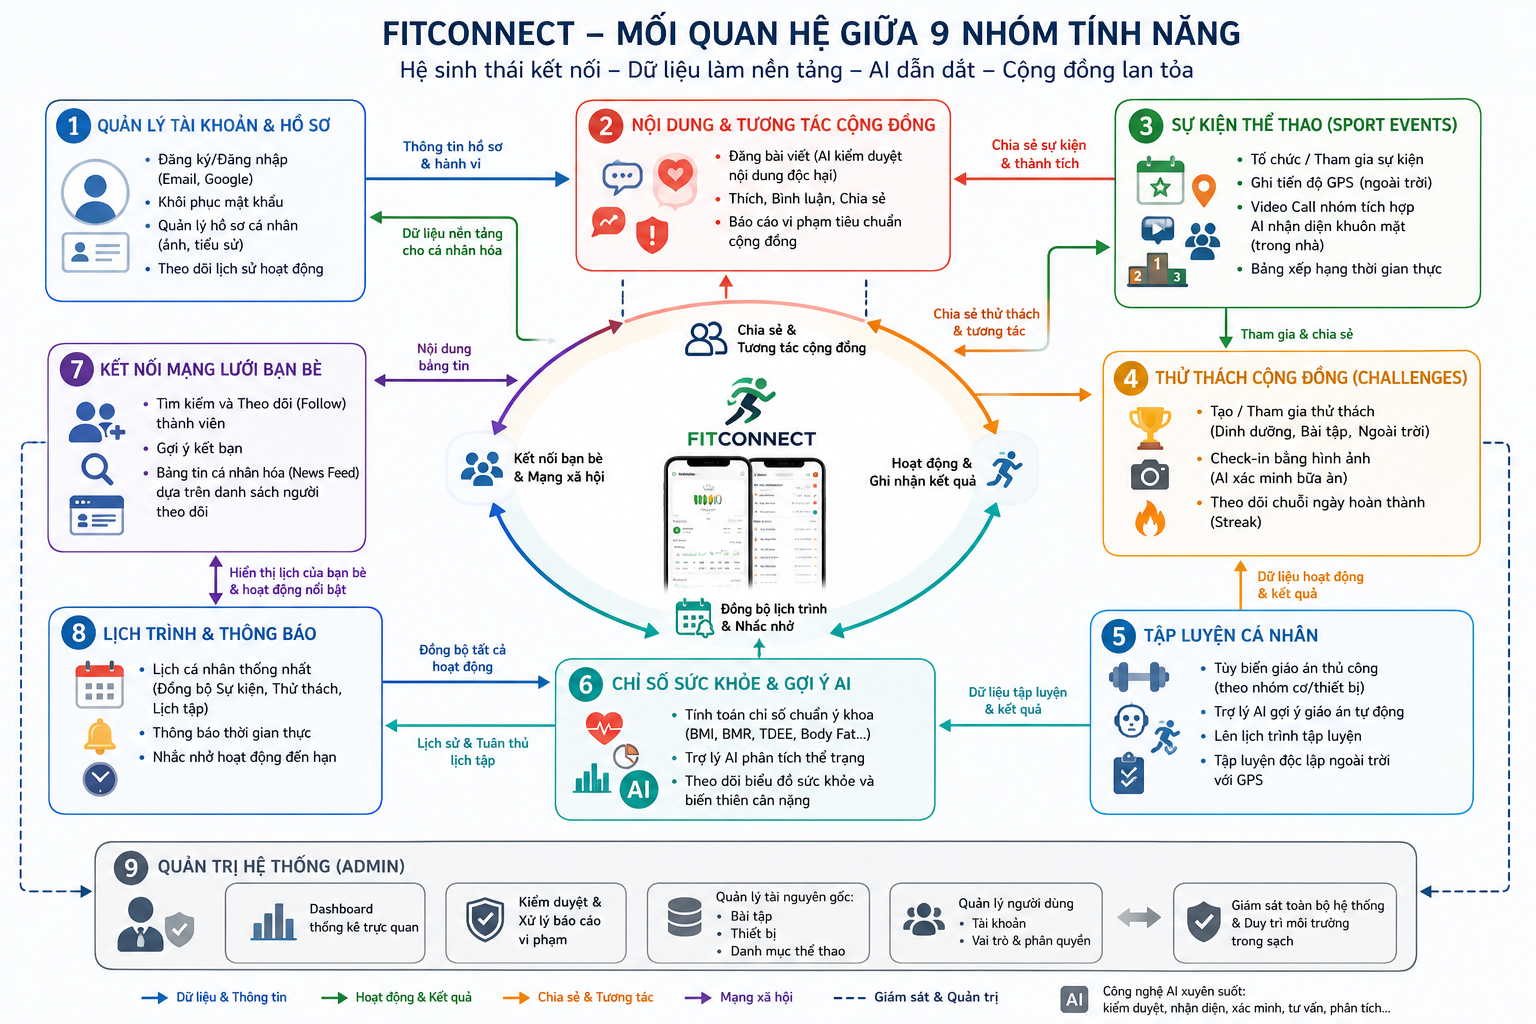
\includegraphics[width=\textwidth]{Images/IMG/Motahethong.png}
\caption{Minh họa khái niệm hệ sinh thái khép kín và mối quan hệ giữa các nhóm tính năng (FitConnect).}
\label{fig:ch1:ecosystem}
\end{figure}

\section{Hiện trạng các nền tảng thể thao -- xã hội và nhu cầu thực tiễn}
\label{sec:intro:platform_status}

Trên bình diện toàn cầu và trong nước, sự giao thoa giữa ``Social'' (mạng xã hội) và ``Fitness'' (thể hình/sức khỏe) đang là xu hướng tất yếu. Các cá nhân tham gia vào hoạt động thể thao thường trải qua ba giai đoạn quá trình tâm lý: \textbf{Khởi đầu (cần hướng dẫn) $\rightarrow$ Duy trì (cần động lực) $\rightarrow$ Tỏa sáng (cần sự công nhận)}\footnote{\href{https://doi.org/10.1186/1479-5868-9-78}{Teixeira et al., IJBNPA, 2012 (động lực \& duy trì hành vi)}}.

\begin{figure}[htbp]
\centering
\setlength{\abovecaptionskip}{14pt}%
\setlength{\belowcaptionskip}{8pt}%
\begin{tikzpicture}[font=\small,
  st/.style={rectangle, draw=black!55, rounded corners=2pt, minimum width=3.6cm, minimum height=1cm, align=center}]
\node[st, fill=gray!12] (s1) at (0,0) {\textbf{Khởi đầu}\\cần hướng dẫn};
\node[st, fill=gray!12] (s2) at (4.8,0) {\textbf{Duy trì}\\cần động lực};
\node[st, fill=gray!12] (s3) at (9.6,0) {\textbf{Tỏa sáng}\\cần sự công nhận};
\draw[->, thick] (s1) -- (s2);
\draw[->, thick] (s2) -- (s3);
\path (current bounding box.south west) ++(0,-0.2) (current bounding box.south east) ++(0,-0.2);
\end{tikzpicture}\par\nobreak\vspace{10pt}\nobreak
\begingroup
\captionsetup{font=footnotesize,labelfont=bf}
\caption{Ba giai đoạn tâm lý thường gặp khi tham gia hoạt động thể thao có hỗ trợ công nghệ.}
\label{fig:ch1:psych-stages}
\endgroup
\end{figure}

Khảo sát thực tiễn cho thấy các ứng dụng hiện hành đang bỏ ngỏ hoặc chưa tối ưu những khoảng trống sau:

\begin{enumerate}
    \item \textbf{Sự kết nối giữa thể dục thể thao ngoài trời (outdoor) và trong nhà (indoor) trong khâu tổ chức sự kiện:} Rất hiếm nền tảng cho phép người dùng chạy bộ ngoài công viên và người dùng đang tập gym tại nhà có thể tham gia chung một ``sự kiện tiến độ cộng đồng'' một cách đồng bộ.

    \item \textbf{Động lực bền bỉ từ thử thách cộng đồng đa dạng:} Các ứng dụng thường chỉ đo lường một loại hình duy nhất. Nhu cầu cần một chuỗi thử thách mạnh mẽ, từ việc kỷ luật \textbf{ăn uống} (có hệ thống AI nhận diện bữa ăn hợp lệ theo thời gian thực), thử thách \textbf{ngoài trời} (đạp xe, chạy bộ) đến lộ trình \textbf{thể dục cá nhân} do AI tư vấn.

    \item \textbf{Cảm giác ``cùng nhau'' từ xa:} Việc tập thể thao ở nhà một mình dễ gây nhàm chán. Nhu cầu kết nối trực tuyến qua luồng video (video call) để tập cùng bạn bè, đồng thời có AI tính toán quy đổi thành điểm số của nhóm là một điểm chạm tương tác chưa được khai thác sâu.

    \item \textbf{Hệ sinh thái thông minh thống nhất:} Ít nền tảng mang lại luồng dữ liệu thông suốt, nơi công cụ tính toán sức khỏe (BMI, TDEE, BMR) chuyển hóa dữ liệu giúp AI chuyên môn gợi ý hệ thống bài tập (workouts) và tự động đồng bộ hóa lên lịch cá nhân (calendar) của người dùng.
\end{enumerate}

Chính bối cảnh này mở ra định hướng thiết kế cốt lõi cho nền tảng FitConnect: \textbf{Lấy tính cộng đồng làm nền tảng, lấy Sự kiện \& Thử thách làm động lực trung tâm, và lấy AI làm công cụ hỗ trợ thông minh.}

\section{Mục tiêu của đề tài}
\label{sec:intro:objectives}

Việc triển khai đề tài hướng tới thỏa mãn các mục tiêu toàn diện ở cả khía cạnh học thuật, công nghệ lẫn ứng dụng thực tiễn:

\begin{enumerate}
    \item \textbf{Mục tiêu sản phẩm:} Xây dựng thành công và đưa vào vận hành hệ thống mạng xã hội thể dục thể thao cộng đồng đa nền tảng (web-based, kiến trúc responsive). Hệ thống phải đảm bảo hoạt động mượt mà, thân thiện với người dùng và xử lý tốt tính liên tục của luồng dữ liệu (news feed, real-time messaging, tracking).

    \item \textbf{Mục tiêu công nghệ \& kỹ thuật:}
    \begin{itemize}
        \item Xây dựng kiến trúc hệ thống hiện đại dựa trên mô hình client--server, áp dụng các tiêu chuẩn thiết kế kiến trúc vi dịch vụ hoặc modular monolithic để mở rộng tính năng dễ dàng.
        \item Ứng dụng trí tuệ nhân tạo (generative AI \& computer vision) một cách sâu rộng vào bài toán thực tiễn: từ việc kiểm tra tính hợp lệ của bài đăng cộng đồng, phân tích hình ảnh nhận diện tiến độ, đến gợi ý lịch trình tập luyện.
        \item Nghiên cứu và hiện thực thành công công nghệ xử lý dữ liệu thời gian thực (real-time GPS tracking, WebSockets cho hệ thống thông báo đa kênh, xử lý đánh giá video stream qua AI)\footnote{\href{https://socket.io/docs/v4/}{Socket.IO docs}; \href{https://datatracker.ietf.org/doc/html/rfc6749}{RFC 6749 (OAuth 2.0)}}.
    \end{itemize}

    \item \textbf{Mục tiêu giá trị xã hội:} Cung cấp một ứng dụng sạch, lành mạnh, tạo ra những cuộc thi/thử thách thể thao mang tính xây dựng, góp phần nâng cao tính kỷ luật, sức khỏe toàn diện cho thanh niên Việt Nam nói riêng và cộng đồng nói chung.
\end{enumerate}

\section{Đối tượng và phạm vi nghiên cứu}
\label{sec:intro:scope}

Để đảm bảo tính khả thi và mức độ hoàn thiện chuyên sâu trong khuôn khổ một đồ án tốt nghiệp, đề tài được giới hạn và phân rã rõ theo các phương diện sau:

\subsection{Đối tượng hướng đến}
\label{subsec:intro:target_audience}

Hệ thống phục vụ đa dạng các tệp người dùng, bao gồm:

\begin{itemize}
    \item \textbf{Người dùng cá nhân:} Những người có nhu cầu chơi thể thao, theo dõi sức khỏe, mong muốn tìm kiếm một lịch trình phù hợp, kết bạn hoặc tham gia các lời mời thử thách.
    \item \textbf{Người khởi xướng sự kiện (event creators/KOLs):} Các hội nhóm thể thao, huấn luyện viên, những nhà hoạt động cộng đồng muốn tổ chức các chiến dịch sức khỏe, phong trào nội bộ hoặc các cuộc thi marathon trực tuyến.
    \item \textbf{Quản trị viên (system admin):} Đội ngũ vận hành hệ thống quản lý dữ liệu master, theo dõi analytics biểu đồ, thực thi kiểm duyệt nội dung và kiểm soát các chỉ số tăng trưởng của nền tảng.
\end{itemize}

\subsection{Phạm vi chức năng}
\label{subsec:intro:functional_scope}

Đồ án tập trung phát triển một hệ thống toàn diện phân rã thành chín nhóm tính năng dành cho người dùng và một phân hệ quản trị (admin), cụ thể:

\subsubsection{Các nhóm tính năng chính}

\begin{enumerate}
    \item \textbf{Cộng đồng:} Xây dựng không gian giao lưu, tương tác mạng xã hội, chia sẻ bài viết, tìm hiểu sự kiện và thử thách. Tích hợp AI tự động kiểm duyệt và nhận diện hình ảnh/nội dung không hợp lệ.

    \item \textbf{Sự kiện thể thao:} Nơi người dùng tạo hoặc tham gia các sự kiện để hoàn thành mục tiêu tập thể. Bao gồm:
    \begin{itemize}
        \item \textbf{Sự kiện ngoài trời:} Hỗ trợ ghi nhận tiến độ bằng GPS tích hợp. Người dùng có thể tham gia sự kiện hoàn thành mục tiêu chung cùng mọi người.
        \item \textbf{Sự kiện trong nhà:} Kết nối thành viên trực tuyến định dạng video call có trợ lực AI nhằm nhận diện và tính toán thời gian vận động thực tế để quy đổi thành tiến độ.
    \end{itemize}

    \item \textbf{Thử thách:} Nền tảng tự rèn luyện cá nhân, nơi người dùng có thể tự tạo hoặc mời bạn bè cùng tham gia. Khác với chức năng sự kiện (tập trung vào mục tiêu tập thể), thử thách đề cao tiến độ bền bỉ mỗi ngày của từng cá nhân. Gồm ba phân loại:
    \begin{itemize}
        \item \textbf{Ăn uống:} Check-in hình ảnh bữa ăn mỗi ngày; hệ thống sử dụng module AI verification đối chiếu hình ảnh để xác thực tính hợp lệ so với yêu cầu đề ra.
        \item \textbf{Ngoài trời:} Ghi lại tiến độ chạy bộ, đạp xe\ldots\ để tiến gần đến mục tiêu cá nhân hằng ngày.
        \item \textbf{Thể dục (gym):} Báo cáo tiến độ hoàn thành các bài tập giúp rèn luyện sức khỏe bản thân.
    \end{itemize}
\end{enumerate}

\subsubsection{Các tính năng bổ trợ quan trọng}

\begin{enumerate}
\setcounter{enumi}{3}
    \item \textbf{Bạn bè:} Quản lý danh sách mạng lưới kết bạn, tăng tính gắn kết trong hệ sinh thái.

    \item \textbf{Tập luyện:} Hệ thống cho phép người dùng tự thiết lập bộ bài tập dựa trên cấu hình tùy chỉnh (thiết bị, nhóm cơ), hoặc nhờ AI cá nhân hóa và gợi ý lộ trình tập. Cung cấp khả năng lưu trữ thành bài tập theo lịch trình dài hạn hoặc các hoạt động ngoài trời độc lập.

    \item \textbf{Công cụ tính toán (calculators):} Bộ công cụ tính các chỉ số sức khỏe sinh học (BMI, BMR, TDEE\ldots), quản lý và hiển thị biểu đồ lịch sử biến động. Dựa vào ngân hàng dữ liệu này, AI insight sẽ tư vấn sức khỏe dựa trên các số đo thực tế và đề xuất phân loại bài tập phù hợp.
    Trong module ước tính tiêu hao năng lượng khi vận động, hệ thống sử dụng công thức quy đổi từ MET sang kcal/phút: $\mathrm{kcal/phút}=\dfrac{MET \times 3.5 \times cân\ nặng\ (kg)}{200}$\footnote{\href{https://pacompendium.com/unite-conversions/}{Compendium of Physical Activities -- Unit Conversions}}. Công thức này dựa trên định nghĩa chuẩn $1\,MET = 3.5\,ml\,O_2/kg/phút$ và quy ước chuyển đổi tiêu hao oxy sang năng lượng, giúp chuẩn hóa cách ước tính giữa các loại hoạt động khác nhau. Nhằm hỗ trợ người dùng phổ thông dễ tra cứu và áp dụng, báo cáo cũng đối chiếu cách diễn giải thực hành từ một tài liệu sức khỏe cộng đồng\footnote{\href{https://howdyhealth.tamu.edu/use-metabolic-equivalents-mets-to-calculate-calories-burned/}{Texas A\&M Howdy Health -- Use METs to Calculate Calories Burned}}.

    \item \textbf{Lịch cá nhân (calendar):} Giao diện lịch biểu hợp nhất, giúp người dùng trực quan hóa lịch trình chéo giữa: thử thách, sự kiện thể thao tham gia và thời khóa biểu các bài tập.

    \item \textbf{Quản lý thông tin cá nhân:} Module authentication, quản lý hồ sơ và các cài đặt tùy biến định danh người dùng.

    \item \textbf{Thông báo:} Kênh notification theo thời gian thực (real-time).
\end{enumerate}

\subsubsection{Phân hệ quản trị (admin panel)}

\begin{enumerate}
\setcounter{enumi}{9}
    \item \textbf{Quản trị hệ thống:} Giao diện dành cho đội ngũ vận hành.
    \begin{itemize}
        \item Cung cấp không gian dashboard trực quan chuyên sâu với các biểu đồ thống kê đa chiều về tình trạng hệ thống.
        \item Công cụ quản lý, trích xuất dữ liệu, kiểm duyệt vi phạm (báo cáo nội dung xấu), ban hành danh mục đối tượng (người dùng, sự kiện, bài viết, đề mục thể thao, tập hợp trang thiết bị thiết yếu, bài tập căn bản và thử thách cộng đồng).
    \end{itemize}
\end{enumerate}

\subsection{Phạm vi kỹ thuật}
\label{subsec:intro:technical_scope}

Kiến trúc hệ thống được xây dựng trên tech-stack hiện đại, tuân thủ các quy tắc design pattern do yêu cầu về tốc độ và chi phí tính toán:

\begin{itemize}
    \item \textbf{Ngôn ngữ và frontend (client-side):} Kiến trúc single page application (SPA) phát triển trên nền tảng ReactJS (sử dụng Vite bundler), tối ưu giao diện component bằng TailwindCSS. Cấu trúc chuyên biệt tách biệt frontend người dùng và frontend quản trị viên\footnote{\href{https://react.dev}{React}; \href{https://vite.dev}{Vite}; \href{https://tailwindcss.com}{Tailwind CSS}}.

    \item \textbf{Backend (API server):} Môi trường Node.js kết hợp TypeScript đảm bảo nguyên tắc type-safe, triển khai qua Express framework theo kiến trúc RESTful kết hợp mô hình lớp controller -- service -- repository\footnote{\href{https://nodejs.org}{Node.js}; \href{https://expressjs.com}{Express}; \href{https://www.typescriptlang.org}{TypeScript}}.

    \item \textbf{Cơ sở dữ liệu (database):} Cấu trúc lõi NoSQL (MongoDB) phục vụ lưu trữ luồng dữ liệu schema-less dạng feed và mạng lưới quan hệ lỏng lẻo của social network\footnote{\href{https://www.mongodb.com/docs/}{MongoDB Documentation}}.

    \item \textbf{Streaming \& công nghệ phụ trợ:} Giao thức WebSockets (Socket.IO) đảm nhận tín hiệu và thông báo thời gian thực; tích hợp API OpenAI cho module đánh giá ngôn ngữ và thị giác. Bảo vệ API có thể áp dụng rate limiting và Helmet\footnote{\href{https://helmetjs.github.io/}{Helmet (HTTP headers, Express)}; \href{https://github.com/express-rate-limit/express-rate-limit}{\texttt{express-rate-limit} (GitHub)}}.
\end{itemize}

\section{Phương pháp nghiên cứu và thực hiện}
\label{sec:intro:methodology}

Quy trình thực hiện đồ án tuân thủ theo chuẩn phát triển phần mềm Agile\footnote{\href{https://agilemanifesto.org}{Agile Manifesto}}, gồm 5 bước: (1)~Nghiên cứu tài liệu về kiến trúc mạng xã hội, thuật toán nhận diện ảnh và prompt engineering; (2)~Khảo sát và đặc tả yêu cầu qua mô hình hóa user personas và use-case; (3)~Thiết kế kiến trúc hệ thống bằng UML (ERD, activity/sequence diagram), phác thảo UI/UX; (4)~Hiện thực theo từng sprint, ánh xạ nghiệp vụ xuống các REST API độc lập; (5)~Kiểm thử toàn diện (unit test, integration test, UAT) đảm bảo độ ổn định và bảo mật.

\section{Bố cục của báo cáo}
\label{sec:intro:structure}

Nội dung cuốn đồ án được tổ chức một cách hệ thống và logic, bao gồm tám chương cụ thể như sau:

\begin{itemize}
    \item \textbf{Chương 1: Giới thiệu đề tài.} Trình bày bối cảnh, lý do chọn đề tài, xác định mục tiêu, đối tượng, phạm vi nghiên cứu và phương pháp thực hiện.

    \item \textbf{Chương 2: Khảo sát hệ thống liên quan.} Đánh giá và phân tích ưu khuyết điểm của các nền tảng mạng xã hội thể thao hiện có trên thị trường, từ đó so sánh và rút ra định hướng thiết kế cốt lõi cho hệ thống FitConnect.

    \item \textbf{Chương 3: Phân tích và đặc tả yêu cầu hệ thống.} Phân tích bài toán thực tế, xác định các tác nhân (actors), lập danh sách các yêu cầu chức năng, phi chức năng và xây dựng biểu đồ use-case bao quát hoạt động.

    \item \textbf{Chương 4: Thiết kế kiến trúc hệ thống.} Cung cấp cái nhìn chuyên sâu về kiến trúc tổng thể, mô hình cơ sở dữ liệu (ERD), thiết kế giao diện (UI/UX) và luồng xử lý dữ liệu qua activity/sequence diagram.

    \item \textbf{Chương 5: Tìm hiểu công nghệ.} Trình bày cơ sở lý thuyết và kỹ thuật áp dụng (Vite/React, Node.js/Express, MongoDB, WebSockets, lý thuyết tích hợp AI và computer vision).

    \item \textbf{Chương 6: Hiện thực hệ thống.} Cụ thể hóa quá trình lập trình thực tế, minh họa cách các phân hệ đi vào hoạt động, những khó khăn thiết kế và giao diện người dùng.

    \item \textbf{Chương 7: Kiểm thử hệ thống.} Trình bày chiến lược kiểm thử, tích hợp các kịch bản test (test cases) nhằm đảm bảo tính đúng đắn, an toàn và hiệu năng thực tế của nền tảng.

    \item \textbf{Chương 8: Tổng kết.} Lập báo cáo kết quả đạt được đối chiếu với mục tiêu đặt ra, tổng kết những khuyết điểm còn tồn đọng và định hướng mở rộng hệ thống trong tương lai.
\end{itemize}


\chapter{KHẢO SÁT HỆ THỐNG LIÊN QUAN}
\renewcommand*{\theHsection}{\theHchapter.\the\value{section}}
% !TeX root = main.tex
\label{chap:background_survey}

Chương này đi sâu khảo sát các nền tảng công nghệ liên quan và hệ thống hóa những cơ sở lý thuyết hoạt động. Dựa trên việc phân tích ưu, nhược điểm của các ứng dụng đi trước, tác giả đề xuất các giải pháp kỹ thuật và định hướng tính năng làm kim chỉ nam xây dựng ``Mạng xã hội rèn luyện thể dục thể thao cộng đồng FitConnect''.

\section{Giới thiệu tổng quan}

\subsection{Nền tảng Thể thao Mạng xã hội khép kín}
Rèn luyện thể chất là quá trình duy trì và nâng cao sức khỏe dài hạn. Trong nhịp sống hiện đại, người dùng thường bị phân mảnh trải nghiệm khi phải cài đặt nhiều ứng dụng rời rạc (app đo GPS chạy bộ riêng, app tính calo riêng, app mạng xã hội riêng). Vì vậy, tích hợp toàn bộ chu trình từ không gian giao lưu kết bạn, tính toán sức khỏe, đến lên lịch tập luyện vào một ``Mạng xã hội khép kín'' duy nhất là giải pháp tối ưu nhằm đảm bảo sự tiện lợi và giữ chân cộng đồng.

\subsection{Cảm hứng Cộng đồng từ Sự kiện và Thử thách}
Việc tập luyện cá nhân độc lập thường dễ dẫn đến sự nhàm chán và bỏ cuộc giữa chừng. Do đó, hạt nhân của FitConnect nằm ở việc tổ chức các Sự kiện nhóm (Sport Events) và Thử thách kỷ luật (Challenges). Khi được hòa mình vào môi trường thi đua thực tiễn (như giải chạy bộ ngoài trời kết nối GPS, hay tập luyện tại nhà cùng nhau qua nền tảng Video Call trực tuyến), sự cọ xát và khích lệ từ cộng đồng sẽ tạo ra động lực tâm lý mạnh mẽ để duy trì lối sống khỏe.

\subsection{Cá nhân hóa lộ trình qua các Chỉ số Sinh trắc học}
Đo lường các chỉ số sức khỏe là bước tiên quyết để định lượng tình trạng cơ thể. Các chỉ số như BMI (Chỉ số khối lượng), BMR (Tỷ lệ trao đổi chất cơ bản) và TDEE (Năng lượng tiêu thụ hàng ngày) giúp nhận diện rõ ràng trạng thái thừa/thiếu hụt calo. Tại nền tảng, những thông số này không xuất hiện chỉ để hiển thị biểu đồ khô khan, mà được biến thành ``dữ liệu đầu vào'' (Input parameters) sống còn nhằm phân tích chuyên sâu cho chu trình tập luyện tiếp theo.

\subsection{Đột phá AI trong Giám sát minh bạch và Trợ lý Ảo}
Đảm bảo tính trung thực trong các phong trào thi đua khai báo từ xa là bài toán vô cùng nan giải. Tích hợp Trí tuệ Nhân tạo (AI) và Thị giác Máy tính (Computer Vision) là lời giải triệt để. AI đảm nhận vai trò bóc tách dữ liệu điểm ảnh chụp các bữa ăn trong Thử thách Dinh dưỡng để xác thực chéo kết quả, cũng như đo lường trực tiếp thời gian vận động thực qua luồng Video Call. Bên cạnh vai trò ``Trọng tài'', mô hình AI Generative còn đóng vai trò ``Huấn luyện viên ảo'', thu thập các biến số y tế (BMI/TDEE) để tự cấu trúc ra chuỗi danh sách các Bài tập (Workouts) logic nhất cho hệ thống Lịch trình.

\subsection{Quản lý dữ liệu người dùng và thống kê biểu đồ}
Việc duy trì một nền tảng sức khỏe đòi hỏi khả năng quản lý khối lượng thông tin lưu trữ đồ sộ và bảo vệ quyền riêng tư cá nhân một cách nghiêm ngặt. Hơn thế nữa, đối với một hệ sinh thái vận động, động lực của người tham gia gắn liền với các mô hình trực quan hóa số liệu. Bằng cách thiết lập hệ thống Dashboard thống kê với các biểu đồ trực quan, người dùng cá nhân có thể dễ dàng nắm bắt sự tiến bộ của bản thân qua từng chu trình. Đồng thời, ở khía cạnh vận hành, hệ thống biểu đồ quản trị giúp đội ngũ Admin có góc nhìn toàn cảnh về tăng trưởng cộng đồng và mức độ hoạt động để kịp thời điều hướng nội dung hệ thống.

\section{Khảo sát các hệ thống tương tự}
Để hiểu rõ hơn về thị trường và học hỏi kinh nghiệm, chúng tôi đã tiến hành khảo sát một số ứng dụng và nền tảng có chức năng tương tự hoặc liên quan:

\subsection{Ứng dụng Strava}

\subsubsection{Giới thiệu}
Strava là một ứng dụng di động nổi tiếng cung cấp tính năng theo dõi hoạt động thể dục thể thao, đặc biệt là chạy bộ và đạp xe. Ứng dụng này sử dụng định vị GPS để theo dõi và ghi lại quãng đường, tốc độ, và các chỉ số sức khỏe tự động. Strava hoạt động giống như một mạng xã hội dành cho người yêu thể thao, nơi họ có thể chia sẻ quá trình tập luyện với bạn bè. Đây chính là nguồn cảm hứng cho nhóm tính năng \textbf{Sự kiện thể thao Ngoài trời} và \textbf{Mạng lưới bạn bè} của hệ thống FitConnect.

\begin{figure}[H]
    \centering
    
\includegraphics[width=0.4\textwidth]{Images/IMG/hethongkhac/strava.jpg}
    \vspace{0.3cm}
    \caption{Giao diện ứng dụng mạng xã hội thể thao Strava}
    \label{fig:survey_strava}
\end{figure}

\subsubsection{Ưu điểm}
Các ưu điểm chính của ứng dụng Strava được liệt kê như bên dưới:
\begin{itemize}
    \item Tính năng theo dõi định vị GPS, tốc độ và quãng đường hoạt động ngoài trời cực kỳ chính xác.
    \item Đồng bộ hóa dễ dàng với nhiều loại đồng hồ thông minh và thiết bị ngoại vi.
    \item Có tính năng Bảng xếp hạng (Leaderboards) giúp người dùng thi đua trên cùng một quãng đường cố định.
    \item Chức năng mạng xã hội tốt, cho phép mọi người theo dõi, bình luận và khích lệ lẫn nhau.
\end{itemize}

\subsubsection{Nhược điểm}
Bên cạnh những ưu điểm nổi bật, Strava vẫn còn một số hạn chế cần cải thiện:
\begin{itemize}
    \item Ứng dụng tập trung hoàn toàn vào các môn thể thao ngoài trời. Các bài tập trong nhà (Gym, Yoga) bị thiếu hụt tính năng phân tích và thi đua tương tự.
    \item Thiếu các tính năng về quản lý dinh dưỡng hay tổ chức thử thách ăn uống (Diet/Nutrition).
    \item Không có tính năng tổ chức các Sự kiện tương tác trực tuyến qua video (Video call).
\end{itemize}

\subsection{Ứng dụng MyFitnessPal}

\subsubsection{Giới thiệu}
MyFitnessPal là một ứng dụng nổi tiếng trong lĩnh vực theo dõi sức khỏe, đặc biệt là quản lý chế độ ăn uống và tính toán lượng Calo. Người dùng có thể ghi lại lượng calo tiêu thụ, theo dõi thông tin dinh dưỡng của thực phẩm với cơ sở dữ liệu khổng lồ. Ứng dụng này chính là nền tảng tham khảo cho nhóm tính năng \textbf{Tính toán chỉ số sức khỏe} và \textbf{Thử thách dinh dưỡng} của FitConnect, nhưng được cải tiến với công nghệ AI nhận diện hình ảnh.

\begin{figure}[H]
    \centering
    
\includegraphics[width=0.4\textwidth]{Images/IMG/hethongkhac/myfitnesspal.png}
    \vspace{0.3cm}
    \caption{Giao diện ứng dụng theo dõi dinh dưỡng MyFitnessPal}
    \label{fig:survey_mfp}
\end{figure}

\subsubsection{Ưu điểm}
Các ưu điểm chính của ứng dụng MyFitnessPal:
\begin{itemize}
    \item Tính toán chi tiết lượng calo đã nạp.
    \item Hỗ trợ nhập liệu bằng cách quét mã vạch (Barcode Scanner).
    \item Có công cụ tính lượng calo cần thiết đề xuất dựa trên mục tiêu cân nặng mong muốn.
\end{itemize}

\subsubsection{Nhược điểm}
Một số hạn chế của hệ thống:
\begin{itemize}
    \item Việc nhập liệu đồ ăn thủ công tốn nhiều thời gian và làm giảm tính hứng thú của người dùng sau một thời gian dài.
    \item Tính năng mạng xã hội chưa đủ mạnh và còn đơn giản dưới hình thức diễn đàn.
    \item Ứng dụng không tự động gợi ý chi tiết lộ trình tập luyện dựa trên calo mà phải sử dụng các phần mềm chuyên tập luyện khác.
    \item Không có kỹ thuật check-in hình ảnh ứng dụng AI thông minh cho các cuộc thi/thử thách trên mạng xã hội.
\end{itemize}

\subsection{Ứng dụng Nike Training Club (NTC)}

\subsubsection{Giới thiệu}
Nike Training Club (NTC) là ứng dụng hướng dẫn tập luyện tại nhà được xây dựng và thiết kế bởi Nike. Ứng dụng cung cấp sẵn hàng trăm bài tập thể lực và rèn luyện theo đa dạng chủ đề và độ khó khác nhau (từ Bodyweight đến dùng Tạ). Đây là nguồn tư liệu phong phú để FitConnect xây dựng nhóm tính năng \textbf{Tập luyện cá nhân} và \textbf{Trợ lý AI gợi ý bài tập}.

\begin{figure}[H]
    \centering
    
\includegraphics[width=0.4\textwidth]{Images/IMG/hethongkhac/ntc.png}
    \vspace{0.3cm}
    \caption{Giao diện ứng dụng tập luyện tại nhà Nike Training Club}
    \label{fig:survey_ntc}
\end{figure}

\subsubsection{Ưu điểm}
\begin{itemize}
    \item Có ngân hàng cơ sở dữ liệu bài tập lớn, được thiết kế bởi các chuyên gia uy tín.
    \item Có video minh họa trực quan rõ nét và sinh động cho từng động tác.
    \item Cho phép người dùng lọc tìm kiếm bài tập dựa trên mục tiêu, nhóm cơ và thời gian rảnh rỗi.
\end{itemize}

\subsubsection{Nhược điểm}
\begin{itemize}
    \item NTC mang xu hướng luyện tập cá nhân độc lập (single-player), không có tính cộng đồng và mạng xã hội.
    \item Ứng dụng không có cơ chế Sự kiện (Events) để người dùng cùng rủ nhau thi đua xem ai hoàn thành được nhiều thời lượng hơn.
    \item Chỉ đơn thuần đếm giờ qua Timer, ứng dụng không nhận diện xem người tập có đang thực hiện thao tác hay không nên không phù hợp để dùng trong các cuộc thi.
\end{itemize}

\section{Tổng kết khảo sát}
Sau khi phân tích ba hệ thống tiêu biểu (Strava, MyFitnessPal và Nike Training Club), chúng tôi nhận thấy mỗi hệ thống đều có điểm mạnh riêng phục vụ cho một bài toán ngách: Strava xuất sắc ở theo dõi ngoài trời, MyFitnessPal vượt trội ở tính toán chế độ ăn, và NTC dẫn đầu ở thiết kế bài tập trong nhà.

Từ những phân tích trên, hệ thống Mạng xã hội rèn luyện thể dục thể thao FitConnect có thể rút ra một số bài học đáng giá nhằm xây dựng một hệ thống hoàn thiện hơn:
\begin{itemize}
    \item \textbf{Nhu cầu về một hệ sinh thái tích hợp:} Người dùng đang phải phân tán thời gian cho nhiều ứng dụng. Cần một nền tảng ``All-in-one'' kết hợp tính năng Sự kiện ngoài trời, Đo lường dinh dưỡng và Bài tập trong nhà.
    \item \textbf{Tầm quan trọng của Cạnh tranh đồng bộ:} Strava thành công vì khía cạnh thi đua (Leaderboard). Các dự án tập luyện trong nhà cũng cần tích hợp cơ chế Sự kiện đồng bộ có tính cạnh tranh tương tự.
    \item \textbf{AI là giải pháp chống gian lận và tối ưu hiệu suất:} Cần áp dụng AI vào trong các thử thách ăn uống (để thay cho việc nhập liệu thủ công chậm chạp) và AI vào Camera khi tập thể thao trong nhà (để đo thời gian thực tế, tính toán thành tích khách quan).
    \item \textbf{Tính cá nhân hóa sâu sắc:} Các chỉ số công cụ tính BMI, TDEE không chỉ sinh ra để hiển thị biểu đồ, mà nên được tái sử dụng để làm thông số đầu vào cho module AI Gợi ý lịch tập luyện (Workout) tiếp theo.
\end{itemize}

\section{Các tính năng cải tiến đề xuất cho hệ thống}
Dựa trên kết quả khảo sát và phân tích các hệ thống hiện có, hệ thống \textbf{FitConnect} đề xuất không chỉ kế thừa những tính năng chuẩn kỹ thuật từ các ứng dụng quốc tế mà còn bổ sung các cải tiến mới mẻ bằng công nghệ thông tin tiên tiến, kết nối cộng đồng một cách chặt chẽ và khách quan. Các đề xuất cải tiến được phân nhóm thành bốn nhóm tính năng chính:

\subsection{Tính năng cộng đồng}
Để biến FitConnect từ một công cụ theo dõi sức khỏe đơn thuần thành một hệ sinh thái mạng xã hội sống động, nền tảng đề xuất tích hợp không gian kết nối chuyên biệt dành cho cộng đồng yêu thích thể thao:
\begin{itemize}
    \item \textbf{Chia sẻ bài viết và thành tích:} Cung cấp môi trường cho phép người dùng tự do đăng tải hình ảnh, cập nhật trạng thái và chia sẻ kết quả tập luyện cá nhân lên bảng tin (News Feed). Qua đó, mỗi cá nhân không chỉ lưu giữ được hành trình rèn luyện của bản thân mà còn dễ dàng nắm bắt các xu hướng sự kiện, thử thách đang thu hút sự chú ý từ cộng đồng.
    \item \textbf{Tương tác đa chiều:} Tăng cường sự gắn kết giữa các thành viên thông qua cơ chế bày tỏ cảm xúc (React) và bình luận (Comment) trực tiếp trên bài viết. Những hoạt động trao đổi, động viên chéo này góp phần xây dựng không gian mạng tích cực, tạo động lực tâm lý mạnh mẽ để duy trì thói quen tập luyện bền lâu.
    \item \textbf{Kết nối mạng lưới bạn bè:} Chức năng kết bạn và theo dõi (Follow) giúp người dùng liên tục cập nhật tin tức từ những người có chung sở thích. Nhờ quan sát lộ trình tập luyện và các hoạt động thể thao mà bạn bè đang tham gia, người dùng dễ dàng nhận lời mời và hòa nhập vào vòng tròn rèn luyện chung.
    \item \textbf{Kiểm duyệt nội dung bằng AI:} Tích hợp module AI tự động quét và kiểm duyệt hình ảnh cùng ngôn từ trong bài viết, kịp thời phát hiện và loại bỏ nội dung vi phạm tiêu chuẩn cộng đồng. Người dùng cũng có thể chủ động báo cáo (Report) các nội dung sai lệch để Quản trị viên xử lý nhanh chóng.
\end{itemize}

\subsection{Tính năng Sự kiện thể thao (Ngoài trời và Trong nhà)}
Khắc phục hạn chế của Strava (chỉ phục vụ ngoài trời) và NTC (thiếu tính cộng đồng), FitConnect đề xuất hệ thống Sự kiện thể thao linh hoạt, phủ sóng đầy đủ cả hai môi trường vận động:
\begin{itemize}
    \item \textbf{Tạo và tham gia sự kiện dễ dàng:} Người dùng có thể tìm kiếm, tham gia vào các sự kiện cộng đồng có sẵn hoặc tự tay khởi tạo sự kiện thi đua mới. Hệ thống tích hợp công cụ AI sinh kịch bản quy tắc tự động, giúp người dùng thiết lập luật chơi và nội dung sự kiện thông minh chỉ từ ý tưởng ban đầu.
    \item \textbf{Sự kiện ngoài trời với định vị GPS thời gian thực:} Đối với các hoạt động di chuyển ngoài trời như chạy bộ hay đạp xe, hệ thống ghi lại lộ trình GPS theo thời gian thực với độ chính xác cao, theo dõi đồng thời quãng đường, tốc độ và lượng calo tiêu thụ. Bảng xếp hạng cộng đồng (Leaderboard) được cập nhật trực tiếp, thúc đẩy tinh thần thi đua minh bạch.
    \item \textbf{Sự kiện trong nhà qua Video Call có giám sát AI:} Đối với các hoạt động tập luyện tại nhà như Yoga hay Cardio, nền tảng cung cấp không gian Video Call nhóm theo thời gian thực. Đặc biệt, luồng camera được tích hợp với mô hình AI nhận diện chuyển động để tự động đo lường thời gian vận động thực tế của từng người, loại bỏ hoàn toàn các hành vi gian lận và đảm bảo tính công bằng cho tất cả người tham gia.
    \item \textbf{Phân tích và chia sẻ kết quả:} Mọi thành tích sau khi hoàn thành sự kiện được biểu đồ hóa và phân tích khách quan. Người dùng có thể chia sẻ kết quả lên bảng tin để lan tỏa cảm hứng và mời thêm bạn bè tham gia các kỳ sự kiện tiếp theo.
\end{itemize}

\subsection{Tính năng Thử thách cộng đồng}
Khác với Sự kiện thể thao hướng đến thi đua nhóm lớn, Thử thách cộng đồng tập trung vào việc xây dựng kỷ luật cá nhân qua các mục tiêu nhỏ hàng ngày. FitConnect đề xuất các cải tiến vượt trội so với hình thức thử thách thủ công truyền thống:
\begin{itemize}
    \item \textbf{Tạo và tham gia thử thách linh hoạt:} Người dùng tự do tạo ra các chiến dịch thử thách về ăn uống, tập luyện hoặc hoạt động ngoài trời. Công cụ AI hỗ trợ tự động sinh kịch bản thử thách phù hợp với mục tiêu cá nhân, giúp thiết lập nhanh chóng mà không cần kinh nghiệm chuyên môn.
    \item \textbf{Check-in tiến độ đa hình thái với xác thực AI:} Nền tảng áp dụng phương thức check-in phù hợp với từng loại thử thách. Với thử thách dinh dưỡng, người dùng chụp ảnh bữa ăn thực tế và AI tự động nhận diện, đánh giá tính hợp lệ — thay thế hoàn toàn việc nhập liệu thủ công chậm chạp. Với thử thách tập luyện hoặc ngoài trời, cơ chế xác thực tương đương với luồng Sự kiện (camera AI hoặc GPS) được áp dụng để đảm bảo tính khách quan.
    \item \textbf{Theo dõi tiến độ và tương tác cộng đồng:} Lịch biểu trực quan giúp người dùng nắm bắt tiến độ của bản thân và mọi người xung quanh mỗi ngày. Hệ thống hỗ trợ bình luận trực tiếp vào từng hoạt động để ghi nhận và tôn vinh sự nỗ lực của nhau.
    \item \textbf{Chia sẻ và báo cáo vi phạm:} Thành tựu thử thách có thể được chia sẻ lên bảng tin để truyền cảm hứng và mời bạn bè cùng tham gia. Cơ chế báo cáo (Report) cho phép cộng đồng phát hiện và gửi cảnh báo các thử thách chứa nội dung không lành mạnh đến Quản trị viên.
\end{itemize}

\subsection{Tính năng tập luyện}
Khắc phục hạn chế của NTC (thiếu tính cộng đồng, không có cá nhân hóa AI) và MyFitnessPal (không gợi ý lộ trình tập), FitConnect đề xuất hệ thống tập luyện cá nhân toàn diện, kết nối liền mạch từ đo lường sức khỏe đến lên lịch thực hiện:
\begin{itemize}
    \item \textbf{Tính toán và theo dõi chỉ số sức khỏe:} Cung cấp bộ công cụ tính BMI, BMR, TDEE chuẩn y khoa từ các thông số cơ thể cơ bản. Lịch sử chỉ số được lưu trữ và hiển thị dưới dạng biểu đồ theo thời gian, giúp người dùng theo dõi sự tiến bộ qua từng tuần, từng tháng để điều chỉnh thói quen kịp thời.
    \item \textbf{Kho bài tập đa dạng và gợi ý AI cá nhân hóa:} Nền tảng xây dựng thư viện bài tập phong phú, phân loại theo nhóm cơ bắp, thiết bị sẵn có và mức độ khó (từ Bodyweight, Cardio đến bài tập Gym chuyên sâu). Từ các chỉ số sức khỏe đo được, AI Generative tự động phân tích thể trạng và gợi ý danh sách bài tập cá nhân hóa tối ưu, đóng vai trò như một Huấn luyện viên ảo riêng của từng người dùng.
    \item \textbf{Lên lịch tập luyện và thông báo nhắc nhở:} Người dùng có thể lưu các bài tập đã chọn vào bộ lịch cá nhân, sắp xếp lịch trình cho từng ngày trong tuần. Hệ thống Push Notification tự động gửi nhắc nhở đúng giờ để đốc thúc duy trì kỷ luật tập luyện đều đặn.
    \item \textbf{Tập luyện ngoài trời độc lập:} Ngoài các bài tập cá nhân tại chỗ, nền tảng tích hợp tính năng ghi nhận hoạt động ngoài trời (chạy bộ, đạp xe) kết hợp GPS, giúp người dùng theo dõi thành tích cá nhân và chuẩn bị nền tảng thể lực cho các Sự kiện, Thử thách cộng đồng tiếp theo.
\end{itemize}




\chapter{PHÂN TÍCH VÀ ĐẶC TẢ YÊU CẦU HỆ THỐNG}
\renewcommand*{\theHsection}{\theHchapter.\the\value{section}}
% !TeX root = main.tex
\label{chap:analysis_requirements}

\section{Yêu cầu chức năng }
Dựa trên mục tiêu và phạm vi, hệ thống FitConnect cần đáp ứng các yêu cầu chức năng chính sau:

\subsection{Quản lý tài khoản và hồ sơ người dùng}
Nhóm tính năng này đảm bảo người dùng tham gia nền tảng và quản lý thông tin cá nhân một cách an toàn và thuận tiện.
\begin{itemize}
    \item \textbf{Đăng ký và Xác thực (FR-01):} Đăng ký tài khoản thông qua Email hoặc Google. Hỗ trợ khôi phục mật khẩu qua Email.
    \item \textbf{Quản lý hồ sơ cá nhân (FR-02):} Xem và cập nhật thông tin cá nhân; quản lý các bài viết đã đăng, sự kiện, thử thách đã tham gia, tập luyện đã tạo,...
\end{itemize}

\subsection{Mạng xã hội cộng đồng}
Nhóm tính năng cộng đồng tạo ra không gian tương tác chuyên biệt cho người yêu thể thao, nơi người dùng có thể trao đổi, chia sẻ các hoạt động, sự kiện, thử thách và tương tác với nhau.
\begin{itemize}
    \item \textbf{Quản lý bài viết (FR-03):} Đăng, chia sẻ, xóa bài viết trên bảng tin cộng đồng. AI hỗ trợ lọc hình ảnh và nội dung không phù hợp khi đăng bài viết.
    \item \textbf{Tương tác xã hội (FR-04):} Thích, bình luận trên bài viết; chia sẻ hoạt động (sự kiện, thử thách) để mọi người cùng tham gia.
    \item \textbf{Báo cáo nội dung vi phạm (FR-05):} Người dùng báo cáo bài viết vi phạm; quản trị viên tiếp nhận và xử lý.
\end{itemize}

\subsection{Sự kiện thể thao (Sport Events)}
Nhóm tính năng sự kiện thể thao cho phép người dùng tổ chức và tham gia các sự kiện thể thao, hướng đến một mục tiêu chung của sự kiện. Hệ thống hỗ trợ cả hai hình thức: hoạt động ngoài trời có theo dõi GPS và hoạt động trong nhà qua video call kết hợp AI.
\begin{itemize}
    \item \textbf{Tổ chức và tham gia sự kiện (FR-06):} Tạo sự kiện (thủ công hoặc AI hỗ trợ tạo) hoặc tham gia sự kiện thể thao (ngoài trời, trong nhà); theo dõi tiến độ cá nhân và chung của sự kiện.
    \item \textbf{Thi đua sự kiện ngoài trời và ghi tiến độ thực (FR-07):} Ghi lộ trình GPS theo thời gian thực; xem quãng đường, thời gian, calo; chia sẻ hoạt động lên cộng đồng.
    \item \textbf{Thi đua sự kiện trong nhà qua Video Call (FR-08):} Video call trực tuyến với mọi người; AI ghi nhận thời gian tham gia hợp lệ; lưu lịch sử buổi tập; chia sẻ hoạt động lên cộng đồng.
    \item \textbf{Chia sẻ và mời tham gia sự kiện (FR-09):} Chia sẻ sự kiện, hoạt động và mời bạn bè, mọi người cùng tham gia.
    \item \textbf{Báo cáo sự kiện vi phạm (FR-10):} Báo cáo sự kiện sai phạm; quản trị viên xử lý.
\end{itemize}

\subsection{Thử thách cộng đồng (Challenges)}
Nhóm tính năng thử thách tập trung vào việc xây dựng kỷ luật cá nhân thông qua các mục tiêu mỗi ngày. Khác với sự kiện thể thao hướng đến mục tiêu chung, thử thách đề cao tiến độ bền bỉ riêng của từng cá nhân theo thời gian.
\begin{itemize}
    \item \textbf{Tạo và tham gia thử thách cộng đồng (FR-11):} Tạo (thủ công hoặc AI hỗ trợ tạo) hoặc tham gia thử thách cộng đồng (ăn uống, tập luyện, ngoài trời).
    \item \textbf{Hoàn thành tiến độ thử thách(FR-12):} Check-in ảnh bữa ăn đối với thử thách ăn uống; Thực hiện tập các bài tập đối với thử thách tập luyện; Đo tiến độ GPS đối với thử thách ngoài trời.
    \item \textbf{Chia sẻ và mời mọi người tham gia (FR-13):} Chia sẻ thử thách, hoạt động và mời bạn bè, mọi người cùng tham gia.
    \item \textbf{Báo cáo vi phạm thử thách (FR-14):} Báo cáo thử thách vi phạm; quản trị viên xử lý.
\end{itemize}

\subsection{Tính toán các chỉ số sức khỏe và gợi ý tập luyện}
Nhóm tính năng này cung cấp bộ công cụ đo lường và theo dõi sức khỏe cá nhân, đồng thời kết hợp trợ lý AI để đưa ra gợi ý tập luyện phù hợp với thể trạng và mục tiêu của từng người dùng.
\begin{itemize}
    \item \textbf{Đo lường các chỉ số sức khỏe (FR-15):} Hệ thống tính toán các chỉ số như BMI, BMR, TDEE và chỉ số liên quan từ thông số cơ thể người dùng nhập.
    \item \textbf{Trợ lý AI phân tích và gợi ý tập luyện (FR-16):} Dựa vào các chỉ số đã tính toán, AI phân tích và gợi ý danh sách các bài tập phù hợp từ danh sách hệ thống bài tập.
    \item \textbf{Theo dõi biểu đồ sức khỏe theo thời gian (FR-17):} Lưu lịch sử chỉ số; hiển thị biểu đồ xu hướng theo thời gian.
\end{itemize}

\subsection{Tập luyện cá nhân}
Nhóm tính năng tập luyện giúp người dùng xây dựng giáo án và duy trì lịch tập cá nhân. Người dùng có thể tự thiết kế bài tập theo nhu cầu hoặc nhận gợi ý tập luyện cá nhân hóa từ AI dựa trên các chỉ số sức khỏe đã đo lường.
\begin{itemize}
    \item \textbf{Tùy biến giáo án thủ công (FR-18):} Dựa vào thiết bị, nhóm cơ muốn tập mà chọn lọc, tùy chỉnh bài tập cho phù hợp.
    \item \textbf{AI gợi ý nhanh bài tập (FR-19):} Nhập mong muốn tập hoặc dựa trên chỉ số sức khỏe, AI gợi ý bộ bài tập phù hợp.
    \item \textbf{Lưu trữ và Lên lịch biểu (FR-20):} Lưu giáo án; xếp lịch tập theo ngày.
    \item \textbf{Rèn luyện thể thao độc lập ngoài trời (FR-21):} Ghi hoạt động ngoài trời (chạy bộ, đạp xe\ldots).
\end{itemize}

\subsection{Kết nối mạng lưới bạn bè}
Nhóm tính năng này xây dựng yếu tố mạng xã hội, giúp người dùng mở rộng mạng lưới quan hệ và duy trì sự gắn kết với những người có chung đam mê thể thao.
\begin{itemize}
    \item \textbf{Theo dõi và Mở rộng mạng lưới (FR-22):} Tìm kiếm, gợi ý, kết bạn hoặc theo dõi thành viên khác.
    \item \textbf{Hoạt động tương tác với bạn bè (FR-23):}  Hoạt động nổi bật (sự kiện, thử thách) của bạn bè hiển thị trên bảng tin.
\end{itemize}

\subsection{Lịch trình cá nhân và thông báo}
Nhóm tính năng này giúp người dùng nắm bắt toàn bộ kế hoạch hoạt động trên một lịch cá nhân thống nhất và nhận được thông báo kịp thời, từ đó duy trì thói quen tập luyện đều đặn.
\begin{itemize}
    \item \textbf{Theo dõi lịch trình hoạt động (FR-24):} Theo dõi lịch sự kiện, thử thách, buổi tập cá nhân mà tôi đã tham gia.
    \item \textbf{Hệ thống thông báo và liên kết bảng tin (FR-25):} Thông báo thời gian thực (nhắc lịch, tương tác bạn bè); có thể đồng bộ hoạt động lên bảng tin.
\end{itemize}

\subsection{Quản trị Hệ thống toàn diện dành cho Quản trị viên}
Phân hệ quản trị cung cấp cho Quản trị viên (Admin) đầy đủ công cụ để giám sát, kiểm soát và vận hành nền tảng một cách hiệu quả, đảm bảo chất lượng nội dung và tính toàn vẹn của dữ liệu hệ thống.
\begin{itemize}
    \item \textbf{Phân tích Dashboard trực quan (FR-26):} Theo dõi, phân tích tình hình hệ thống dựa trên các biểu đồ dashboard.
    \item \textbf{Kiểm soát và Xử lý vi phạm (FR-27):} Xử lý báo cáo; xóa bài viết, sự kiện, thử thách, tài khoản vi phạm.
    \item \textbf{Quản lý toàn diện tài nguyên hệ thống (FR-28):} Truy vấn, chỉnh sửa dữ liệu người dùng, sự kiện, thử thách, danh mục bài tập và cấu hình liên quan.
\end{itemize}

\section{Yêu cầu phi chức năng}
\phantomsection\label{sec:req:nfr_manual}

Bên cạnh yêu cầu chức năng, FitConnect cần đáp ứng các yêu cầu phi chức năng để bảo đảm hiệu năng, an toàn, độ tin cậy và trải nghiệm sử dụng thực tế. Bảng~\ref{tab:nfr_summary} tóm tắt các yêu cầu chính.

% Bảng vừa một trang: dùng table+tabular thay vì longtable để tránh lỗi tách trang
% ``Infinite glue shrinkage found in box being split'' (longtable + \small/\arraystretch).
\begin{table}[H]
\centering
\caption{Tổng hợp yêu cầu phi chức năng hệ thống FitConnect}\label{tab:nfr_summary}
\small
\renewcommand{\arraystretch}{1.15}
\begin{tabular}{|p{3.6cm}|p{10.4cm}|}
\hline
\textbf{Tiêu chí} & \textbf{Yêu cầu chính} \\
\hline
\textbf{Hiệu năng} (Performance) &
Thời gian phản hồi API chính (p95) $\leq$ 2 giây; truy vấn nặng (tìm kiếm/tổng hợp) $\leq$ 3 giây. Hệ thống hỗ trợ tối thiểu 1.000 người dùng đồng thời (theo kịch bản Loader.io) và độ trễ thông báo thời gian thực (WebSocket) trung bình $\leq$ 1 giây. \\
\hline
\textbf{Bảo mật} (Security) &
100\% giao tiếp qua HTTPS; mật khẩu băm Bcrypt (cost factor $\geq$ 10). Access Token hết hạn sau 15 phút, Refresh Token tối đa 7 ngày; khóa tạm 15 phút sau 5 lần đăng nhập sai liên tiếp; rate limiting tối thiểu 100 request/15 phút/IP cho endpoint nhạy cảm; 100\% route quản trị yêu cầu JWT hợp lệ và vai trò Admin. \\
\hline
\textbf{Khả dụng \& Tin cậy} (Availability) &
Mục tiêu uptime dịch vụ $\geq$ 99.5\%/tháng; sao lưu dữ liệu tự động hằng ngày; RPO $\leq$ 24 giờ và RTO $\leq$ 4 giờ khi xảy ra sự cố nghiêm trọng. \\
\hline
\textbf{Mở rộng} (Scalability) &
Hỗ trợ mở rộng ngang tối thiểu 2--3 instance backend sau reverse proxy mà không thay đổi nghiệp vụ; khi tải tăng gấp 2 lần, thời gian phản hồi p95 không vượt quá 3 giây. \\
\hline
\textbf{Tương thích} (Compatibility) &
Responsive cho độ rộng màn hình từ 375px trở lên; hỗ trợ Chrome, Edge, Firefox, Safari ở 2 phiên bản ổn định gần nhất tại thời điểm phát hành. \\
\hline
\textbf{Khả năng sử dụng} (Usability) &
Người dùng mới hoàn thành các tác vụ cốt lõi (đăng ký, tạo bài viết, tham gia sự kiện/thử thách) trong $\leq$ 3 phút mỗi tác vụ; luồng chính không quá 5 thao tác từ màn hình chính. \\
\hline
\textbf{Bảo trì \& Chất lượng mã} (Maintainability) &
Frontend/backend dùng TypeScript và phân tầng rõ ràng; duy trì kiểm thử cho module quan trọng với độ bao phủ tối thiểu 85\% (unit + integration), lint/build phải đạt 100\% trước khi phát hành. \\
\hline
\end{tabular}
\end{table}

\section{Lược đồ Use Case}
Lược đồ Use Case (Tham khảo Hình~\ref{fig:usecase_tong_quat}) trình bày bức tranh tổng thể các chức năng của hệ thống FitConnect dưới góc nhìn của các tác nhân sử dụng. Hai tác nhân chính gồm \textbf{Người dùng (User)} và \textbf{Quản trị viên (Administrator)} với các quyền và phạm vi thao tác khác nhau.

\begin{figure}[H]
    \centering
    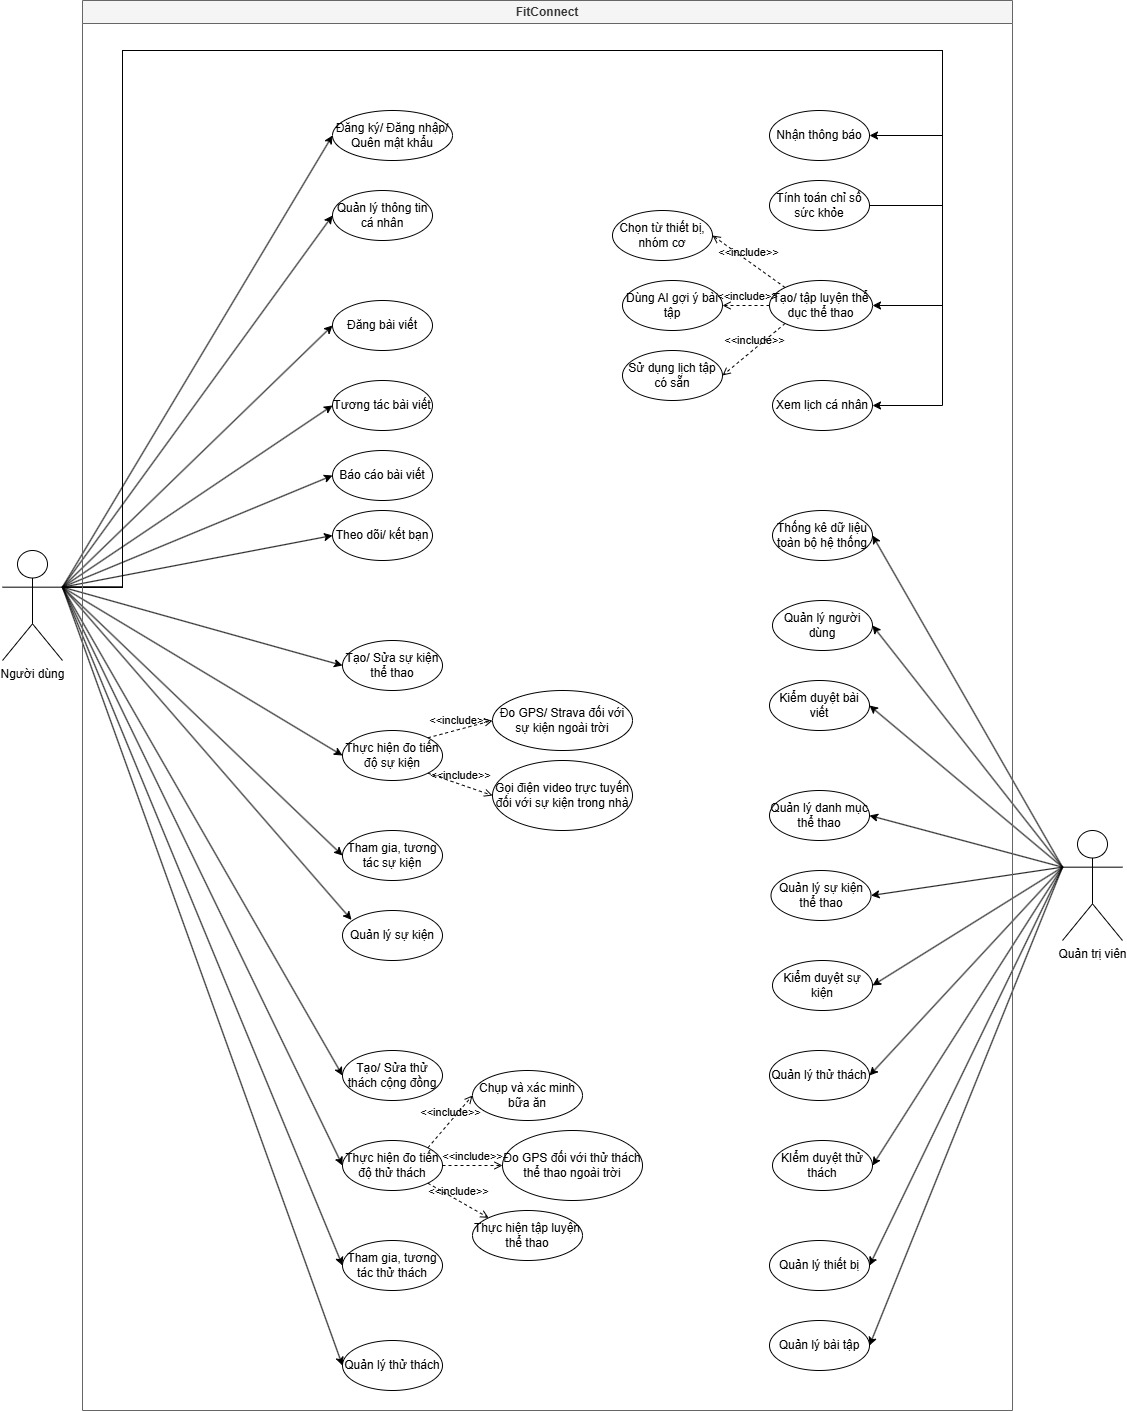
\includegraphics[width=1\textwidth]{Images/IMG/ERD/USECASEDIAGRAMHethong.jpg}
    \vspace{0.5em}
    \caption{Lược đồ Use Case của hệ thống FitConnect}
    \label{fig:usecase_tong_quat}
\end{figure}

Trong lược đồ Use Case, \textbf{Người dùng} có thể quản lý tài khoản, tham gia hoạt động cộng đồng, theo dõi sức khỏe -- tập luyện, đăng ký sự kiện thể thao và tham gia thử thách,... 
\textbf{Quản trị viên} có thể quản trị hệ thống, kiểm duyệt nội dung vi phạm và quản lý các tài nguyên vận hành. Sự phân tách này giúp làm rõ phạm vi chức năng, vai trò của từng tác nhân trong hệ thống.

Đặc tả chi tiết cho 15 trường hợp Use Case được trình bày tại Phụ lục~\ref{sec:usecase_detail} của báo cáo.


\chapter{THIẾT KẾ KIẾN TRÚC HỆ THỐNG}
\renewcommand*{\theHsection}{\theHchapter.\the\value{section}}
\label{chap:system_design}

\section{Thiết kế kiến trúc hệ thống}
\label{sec:architecture_design}

Kiến trúc hệ thống xác định cấu trúc, các thành phần chính và mối quan hệ giữa chúng, nhằm đáp ứng các yêu cầu chức năng và phi chức năng. Hệ thống được thiết kế theo mô hình Client-Server với REST API module hóa, đảm bảo hiệu quả phát triển và dễ bảo trì.

\subsection{Kiến trúc tổng quan (Client-Server với REST API)}
\label{subsec:current_architecture_description}

Hệ thống tuân theo mô hình phân lớp client-server, Frontend là SPA (Single Page Application) giao tiếp với Backend qua REST API.

\begin{figure}[H]
    \centering
    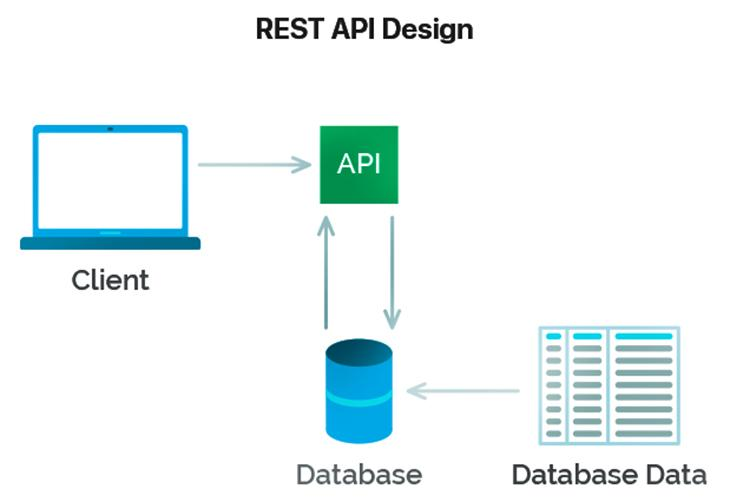
\includegraphics[width=0.75\textwidth]{Images/API.jpg}
    \vspace{1em}
    \caption{Mô hình kiến trúc Client-Server với REST API \cite{MicrosoftLearnClientServerImg}.}
    \label{fig:rest_api_architecture}
\end{figure}

\subsubsection{Frontend (Client)}
\label{subsubsec:frontend_component}
Frontend là lớp giao diện trực tiếp với người dùng, được xây dựng dưới dạng Single Page Application (SPA) để mang lại trải nghiệm mượt mà và nhanh chóng. Việc sử dụng React 18 kết hợp với các thư viện hiện đại như TanStack React Query cho quản lý state và Tailwind CSS cho styling giúp tăng tốc quá trình phát triển và đảm bảo chất lượng code.

Frontend được xây dựng bằng React 18 với các công nghệ chính:
\begin{itemize}
    \item \textbf{Core:} React 18, Vite (build tool), React Router Dom
    \item \textbf{API \& State:} Axios, TanStack React Query
    \item \textbf{Form:} React Hook Form, Yup validation
    \item \textbf{UI:} Tailwind CSS, DaisyUI
\end{itemize}
Cấu trúc thư mục: `pages`, `components`, `apis`, `contexts`, `hooks`, `utils`.

\subsubsection{Backend (Server)}
\label{subsubsec:backend_component}
Backend chịu trách nhiệm xử lý logic nghiệp vụ, quản lý dữ liệu và cung cấp API cho Frontend. Kiến trúc RESTful API module hóa giúp tách biệt rõ ràng các chức năng, dễ bảo trì và mở rộng. Việc sử dụng Node.js với Express.js không chỉ đảm bảo hiệu năng cao mà còn tạo sự đồng nhất ngôn ngữ JavaScript giữa Frontend và Backend, giúp đội ngũ phát triển làm việc hiệu quả hơn.

Backend xây dựng bằng Node.js và Express.js, cung cấp RESTful API module hóa:
\begin{itemize}
    \item \textbf{Nền tảng:} Node.js, Express.js, TypeScript
    \item \textbf{CSDL:} MongoDB (Mongoose ODM)
    \item \textbf{Xác thực:} JWT (JSON Web Tokens)
\end{itemize}

\textbf{Cấu trúc API Backend:} Các API được tổ chức theo tài nguyên:
\begin{itemize}
    \item `/api/auth`: Đăng ký, đăng nhập, bảo mật JWT
    \item `/api/users`: Quản lý hồ sơ, định danh tài khoản
    \item `/api/posts`, `/api/comments`: Quản lý bài đăng, phản hồi và mạng xã hội
    \item `/api/sport-events`: Quản lý sự kiện thể thao (tạo, chia sẻ, lưu tiến độ)
    \item `/api/challenges`: Quản trị chiến dịch thử thách cộng đồng
    \item `/api/workouts`, `/api/exercises`: Điều hướng bài tập và giáo án riêng
    \item `/api/ai`: Điều phối sinh thực thể từ Prompt, đo lường video camera
    \item `/api/calculator`: Tính toán sinh lý học (BMI, TDEE, BMR)
    \item `/api/calendar`: Đồng bộ trung tâm thời gian thực các sự kiện thể thao
    \item `/api/search`: Tìm kiếm truy vấn tổng hợp
    \item `/api/notifications`: Khởi tạo và phát luồng cảnh báo
\end{itemize}

\subsubsection{Cơ sở dữ liệu và Dịch vụ bổ trợ}
\label{subsubsec:database_support_services}
Lớp dữ liệu đóng vai trò quan trọng trong việc lưu trữ và quản lý thông tin. MongoDB được lựa chọn nhờ tính linh hoạt của schema, phù hợp với cấu trúc dữ liệu đa dạng của hệ thống mạng xã hội. Cloudinary cung cấp giải pháp lưu trữ ánh và video chuyên nghiệp, tự động tối ưu hóa và phân phối qua CDN toàn cầu, giúp giảm tải cho server chính và tăng tốc độ tải trang.

\begin{itemize}
    \item \textbf{MongoDB:} Lưu trữ chính cho toàn bộ hệ sinh thái dữ liệu (người dùng, bài đăng, sự kiện, thử thách, bài tập, tiến trình đồng bộ).
    \item \textbf{Cloudinary:} Dịch vụ lưu trữ đám mây cho hình ảnh, video.
\end{itemize}

% \subsection{Sơ đồ kiến trúc tổng quan hiện tại}
% \label{subsec:current_architecture_diagram}

% Sơ đồ dưới đây minh họa mối quan hệ giữa các thành phần chính trong kiến trúc hiện tại của hệ thống:

% \begin{figure}[H]
%     \centering
%     \includegraphics[width=0.9\textwidth]{Images/overall_architecture.png} % Thay bằng đường dẫn ảnh của bạn
%     \caption{Kiến trúc tổng thể hệ thống Nutrition Community Network (Nguồn: AWS Whitepapers - Minh họa)}
%     \label{fig:overall_architecture}
% \end{figure}
% *(Sơ đồ này cần thể hiện rõ: Client (React App) -> Giao tiếp qua REST API -> Backend (Node.js/Express - Module hóa) -> Tương tác với MongoDB, Redis, Cloudinary, và Socket.IO Server)*

% % \subsection{Luồng tương tác ví dụ: Tạo công thức nấu ăn}
% % \label{subsec:interaction_flow_recipe}

% % Luồng tương tác chi tiết khi người dùng tạo một công thức nấu ăn mới:

% % \begin{figure}[H]
% %     \centering
% %     \includegraphics[width=0.9\textwidth]{Images/interaction_flow.png} % Thay bằng đường dẫn ảnh của bạn
% %     \caption{Luồng tương tác giữa các thành phần khi tạo công thức (Minh họa)}
% %     \label{fig:interaction_flow}
% % \end{figure}

% % \begin{enumerate}
% %     \item \textbf{Người dùng (React App)} điền thông tin công thức (tên, nguyên liệu, hướng dẫn...) và chọn hình ảnh vào form.
% %     \item \textbf{React App (Client-side Validation)} sử dụng React Hook Form và Yup để kiểm tra tính hợp lệ của dữ liệu nhập.
% %     \item \textbf{React App (Image Upload)} gửi yêu cầu tải hình ảnh lên Cloudinary/Firebase Storage API.
% %     \item \textbf{Cloudinary/Firebase} xử lý, lưu trữ ảnh và trả về URL của ảnh đã lưu.
% %     \item \textbf{React App (API Request)} nhận URL ảnh, đóng gói dữ liệu công thức cùng URL ảnh và gửi yêu cầu POST đến `/api/recipes` trên \textbf{Backend Server}, kèm theo JWT token trong header Authorization.
% %     \item \textbf{Backend Server (Middleware)} xác thực JWT token.
% %     \item \textbf{Backend Server (Controller/Service)} nhận dữ liệu, thực hiện validation phía server.
% %     \item \textbf{Backend Server (Database Interaction)} lưu thông tin công thức mới vào collection `recipes` trong \textbf{MongoDB}.
% %     \item \textbf{Backend Server (Notification Logic - Async)} (Có thể) tạo bản ghi thông báo trong collection `notifications` và đẩy sự kiện "new_recipe" đến \textbf{Socket.IO Server}.
% %     \item \textbf{Socket.IO Server} phát thông báo "new_recipe" đến các client đang kết nối (ví dụ: những người theo dõi người đăng).
% %     \item \textbf{Backend Server} trả về phản hồi thành công (HTTP 201 Created) cho \textbf{React App}, kèm theo dữ liệu công thức vừa tạo (hoặc chỉ ID).
% %     \item \textbf{React App} nhận phản hồi, hiển thị thông báo thành công và điều hướng người dùng đến trang chi tiết công thức mới.
% % \end{enumerate}

\section{Thiết kế cơ sở dữ liệu}
\label{sec:database_design}

Hệ thống sử dụng \textbf{MongoDB} --- cơ sở dữ liệu NoSQL hướng tài liệu. Dữ liệu được tổ chức thành các \textbf{collection}, mỗi collection chứa nhiều \textbf{document} dạng JSON/BSON linh hoạt. Quan hệ giữa các collection thực hiện qua \textbf{referencing} (lưu \texttt{ObjectId}) hoặc \textbf{embedding} (nhúng sub-document trực tiếp). Schema được định nghĩa và validate qua \textbf{Mongoose ODM}.

Phần này trình bày 13 collection cốt lõi của hệ thống FitConnect cùng document ví dụ tương ứng.

% ─── 1. USERS ────────────────────────────────────────────────────────────────
\subsection{Collection \texttt{users}}
\label{subsec:col_users}

Là trung tâm tham chiếu của toàn hệ thống. Lưu thông tin tài khoản, hồ sơ cá nhân và hồ sơ sức khỏe (BMI, BMR, TDEE). Lịch sử biến động chỉ số được nhúng trực tiếp vào document dưới dạng mảng để vẽ biểu đồ xu hướng mà không cần truy vấn collection riêng.

\begin{minted}[frame=single, framesep=2mm, fontsize=\small, bgcolor=backcolour, breaklines, linenos]{javascript}
{
  "_id": ObjectId("681c1a12ab45ef001234abcd"),
  "name": "Nguyen Van A",
  "user_name": "vana",
  "email": "vana@gmail.com",
  "password": "$2b$10$...",
  "avatar": "https://res.cloudinary.com/.../avatar.png",
  "cover_avatar": "https://res.cloudinary.com/.../cover.png",
  "birthday": "2000-03-15T00:00:00Z",
  "gender": "male",
  "address": "TP. Ho Chi Minh",
  "role": 0,
  "status": 1,
  "auth_provider": "local",
  "weight": 68,
  "height": 170,
  "age": 26,
  "hip": 92,
  "waist": 78,
  "neck": 37,
  "activity_level": 2,
  "activity_level_text": "Tap luyen nhe 1-3 ngay/tuan",
  "BMI": 23.5,
  "BMR": 1680,
  "TDEE": 2310,
  "body_fat": 18.2,
  "IBW": 63.5,
  "LBM": 55.6,
  "health_goal": "Giam can",
  "dietary_preferences": "Low-carb",
  "allergies": "",
  "pre_weight": [
    { "weight": 72, "date": "2026-01-01" },
    { "weight": 68, "date": "2026-04-01" }
  ],
  "pre_BMI": [
    { "value": 24.9, "date": "2026-01-01" },
    { "value": 23.5, "date": "2026-04-01" }
  ],
  "isDeleted": false,
  "createdAt": "2026-01-10T08:00:00Z",
  "updatedAt": "2026-05-09T10:30:00Z"
}
\end{minted}

% ─── 2. REFRESH TOKENS ───────────────────────────────────────────────────────
\subsection{Collection \texttt{refresh\_tokens}}
\label{subsec:col_refresh_tokens}

Quản lý phiên đăng nhập bảo mật theo cơ chế JWT Refresh Token. Mỗi thiết bị/phiên đăng nhập tạo ra một document riêng. Index TTL tự động xóa token hết hạn. Khi đăng xuất, document bị xóa để thu hồi quyền truy cập.

\begin{minted}[frame=single, framesep=2mm, fontsize=\small, bgcolor=backcolour, breaklines, linenos]{javascript}
{
  "_id": ObjectId("681c1b23bc56fg001234bcde"),
  "user_id": ObjectId("681c1a12ab45ef001234abcd"),
  "token": "eyJhbGciOiJIUzI1NiIsInR5cCI6IkpXVCJ9...",
  "iat": "2026-05-09T10:30:00Z",
  "exp": "2026-06-09T10:30:00Z",
  "createdAt": "2026-05-09T10:30:00Z"
}
\end{minted}

% ─── 3. POSTS ────────────────────────────────────────────────────────────────
\subsection{Collection \texttt{posts}}
\label{subsec:col_posts}

Lưu bài viết trên bảng tin cộng đồng. Hỗ trợ chia sẻ lại bài viết qua \texttt{parent\_id}. Báo cáo vi phạm nhúng trực tiếp vào document. Lượt thích và bình luận lưu ở các collection riêng (\texttt{like\_posts}, \texttt{comment\_posts}).

\begin{minted}[frame=single, framesep=2mm, fontsize=\small, bgcolor=backcolour, breaklines, linenos]{javascript}
{
  "_id": ObjectId("681c2b34cd56ef001234bcde"),
  "user_id": ObjectId("681c1a12ab45ef001234abcd"),
  "content": "Hom nay chay bo 5km sau 30 phut, ca ngay nang luong!",
  "type": 0,
  "status": 1,
  "is_banned": false,
  "parent_id": null,
  "meal_plan_id": null,
  "report_post": [
    {
      "user_id": ObjectId("681c1a12ab45ef001234efgh"),
      "reason": "Noi dung khong phu hop",
      "created_at": "2026-05-09T08:00:00Z"
    }
  ],
  "createdAt": "2026-05-09T07:00:00Z",
  "updatedAt": "2026-05-09T07:00:00Z"
}
\end{minted}

% ─── 4. LIKE_POSTS & COMMENT_POSTS ───────────────────────────────────────────
\subsection{Collection \texttt{like\_posts} và \texttt{comment\_posts}}
\label{subsec:col_interactions}

\texttt{like\_posts} ghi nhận lượt thích, đảm bảo mỗi người dùng chỉ thích một bài một lần qua index unique \texttt{(user\_id, post\_id)}. \texttt{comment\_posts} lưu bình luận phân cấp, hỗ trợ reply lồng nhau qua \texttt{parent\_comment\_id}.

\begin{minted}[frame=single, framesep=2mm, fontsize=\small, bgcolor=backcolour, breaklines, linenos]{javascript}
// Collection: like_posts
{
  "_id": ObjectId("681c2c45de67ef001234cdef"),
  "user_id": ObjectId("681c1a12ab45ef001234efgh"),
  "post_id": ObjectId("681c2b34cd56ef001234bcde"),
  "createdAt": "2026-05-09T07:05:00Z"
}

// Collection: comment_posts
{
  "_id": ObjectId("681c2d56ef78fg001234defg"),
  "user_id": ObjectId("681c1a12ab45ef001234efgh"),
  "post_id": ObjectId("681c2b34cd56ef001234bcde"),
  "content": "Tuyet voi! Minh cung moi chay xong buoi sang",
  "parent_comment_id": null,
  "is_banned": false,
  "createdAt": "2026-05-09T07:10:00Z"
}
\end{minted}

% ─── 5. FOLLOWS ──────────────────────────────────────────────────────────────
\subsection{Collection \texttt{follows}}
\label{subsec:col_follows}

Mô hình hóa quan hệ theo dõi một chiều giữa người dùng (Social Graph). Mỗi document là một cạnh có hướng \texttt{user\_id → follow\_id}, phục vụ lọc bảng tin ưu tiên nội dung từ người mình theo dõi.

\begin{minted}[frame=single, framesep=2mm, fontsize=\small, bgcolor=backcolour, breaklines, linenos]{javascript}
{
  "_id": ObjectId("681c3c45de67fg001234cdef"),
  "user_id": ObjectId("681c1a12ab45ef001234abcd"),
  "follow_id": ObjectId("681c1a12ab45ef001234efgh"),
  "createdAt": "2026-05-09T08:00:00Z"
}
\end{minted}

% ─── 6. SPORT EVENTS ─────────────────────────────────────────────────────────
\subsection{Collection \texttt{sport\_events}}
\label{subsec:col_sport_events}

Lưu thông tin sự kiện thể thao tập thể. Hỗ trợ hai hình thức: Ngoài trời (theo dõi GPS) và Trong nhà (Video Call + AI điểm danh khuôn mặt). Danh sách người tham gia lưu dạng mảng ObjectId nhúng để kiểm tra trạng thái tham gia nhanh.

\begin{minted}[frame=single, framesep=2mm, fontsize=\small, bgcolor=backcolour, breaklines, linenos]{javascript}
{
  "_id": ObjectId("681c4d56ef78gh001234defg"),
  "name": "Chay Bo Sang Som Quan 1",
  "description": "Su kien chay bo the duc buoi sang...",
  "detailedDescription": "...",
  "category": "Chay bo",
  "eventType": "Ngoai troi",
  "startDate": "2026-05-15T05:30:00Z",
  "endDate": "2026-05-15T07:00:00Z",
  "location": "Online",
  "address": "Cong Vien Le Van Tam, Q.1, TP.HCM",
  "distance": "5km",
  "maxParticipants": 50,
  "participants": 12,
  "image": "https://res.cloudinary.com/.../event.jpg",
  "createdBy": ObjectId("681c1a12ab45ef001234abcd"),
  "organizer": "CLB The Thao ABC",
  "targetValue": 5,
  "targetUnit": "km",
  "difficulty": "easy",
  "requirements": "Giay chay bo, ao the thao",
  "benefits": "Cai thien suc khoe, ket ban",
  "participants_ids": [
    ObjectId("681c1a12ab45ef001234abcd"),
    ObjectId("681c1a12ab45ef001234efgh")
  ],
  "isDeleted": false,
  "createdAt": "2026-05-09T09:00:00Z"
}
\end{minted}

% ─── 7. SPORT EVENT PROGRESS ─────────────────────────────────────────────────
\subsection{Collection \texttt{sport\_event\_progress}}
\label{subsec:col_event_progress}

Ghi nhận kết quả thi đua của từng người dùng trong từng buổi sự kiện. Hỗ trợ ba nguồn: GPS tự động, Video Call và nhập tay. Phục vụ bảng xếp hạng nội bộ sự kiện.

\begin{minted}[frame=single, framesep=2mm, fontsize=\small, bgcolor=backcolour, breaklines, linenos]{javascript}
{
  "_id": ObjectId("681c5e67fg89hi001234efgh"),
  "eventId": ObjectId("681c4d56ef78gh001234defg"),
  "userId": ObjectId("681c1a12ab45ef001234abcd"),
  "date": "2026-05-15T07:05:00Z",
  "value": 5.2,
  "unit": "km",
  "distance": 5200,
  "time": "28:45",
  "calories": 312,
  "activeSeconds": 1725,
  "source": "gps",
  "proofImage": "https://res.cloudinary.com/.../proof.jpg",
  "notes": "Hoan thanh trong 28 phut 45 giay",
  "is_deleted": false,
  "createdAt": "2026-05-15T07:05:00Z"
}
\end{minted}

% ─── 8. ACTIVITY TRACKING ────────────────────────────────────────────────────
\subsection{Collection \texttt{activity\_tracking}}
\label{subsec:col_activity_tracking}

Ghi nhận hoạt động ngoài trời theo thời gian thực qua GPS. Mảng \texttt{gpsRoute} nhúng toàn bộ chuỗi tọa độ để vẽ lại lộ trình. Liên kết với \texttt{sport\_events} hoặc \texttt{challenges} tùy mục đích sử dụng.

\begin{minted}[frame=single, framesep=2mm, fontsize=\small, bgcolor=backcolour, breaklines, linenos]{javascript}
{
  "_id": ObjectId("681c5f78gh90ij001234fghi"),
  "userId": ObjectId("681c1a12ab45ef001234abcd"),
  "eventId": ObjectId("681c4d56ef78gh001234defg"),
  "challengeId": null,
  "activityType": "Chay bo",
  "name": "Chay buoi sang 15/05",
  "status": "completed",
  "startTime": "2026-05-15T05:32:00Z",
  "endTime": "2026-05-15T06:01:00Z",
  "totalDuration": 1725,
  "totalDistance": 5200,
  "avgSpeed": 10.8,
  "maxSpeed": 14.2,
  "avgPace": 5.55,
  "calories": 312,
  "gpsRoute": [
    { "lat": 10.7769, "lng": 106.7009, "timestamp": 1747280000, "speed": 10.5 },
    { "lat": 10.7772, "lng": 106.7015, "timestamp": 1747280030, "speed": 11.2 }
  ],
  "pauseIntervals": [],
  "source": "app",
  "createdAt": "2026-05-15T05:32:00Z"
}
\end{minted}

% ─── 9. CHALLENGES ───────────────────────────────────────────────────────────
\subsection{Collection \texttt{challenges}}
\label{subsec:col_challenges}

Lưu thông tin thử thách rèn luyện kỷ luật ngắn hạn (dinh dưỡng, bài tập hoặc ngoài trời). Danh sách bài tập yêu cầu (loại fitness) được nhúng trực tiếp. Hỗ trợ tạo thủ công hoặc AI đề xuất.

\begin{minted}[frame=single, framesep=2mm, fontsize=\small, bgcolor=backcolour, breaklines, linenos]{javascript}
{
  "_id": ObjectId("681c6f78gh90ij001234fghi"),
  "title": "30 Ngay Plank Moi Ngay",
  "description": "Ren luyen core moi sang, bat dau tu 30 giay",
  "image": "https://res.cloudinary.com/.../challenge.jpg",
  "creator_id": ObjectId("681c1a12ab45ef001234abcd"),
  "challenge_type": "fitness",
  "category": "Core training",
  "goal_type": "duration",
  "goal_value": 60,
  "goal_unit": "giay",
  "kcal_per_unit": 0.15,
  "start_date": "2026-05-10T00:00:00Z",
  "end_date": "2026-06-09T23:59:59Z",
  "visibility": "public",
  "is_public": true,
  "status": "active",
  "difficulty": "medium",
  "badge_emoji": "\ud83c\udfc6",
  "participants_count": 128,
  "exercises": [
    {
      "exercise_id": ObjectId("681caa11bb22cc001234aabb"),
      "exercise_name": "Plank",
      "sets": [{ "set_number": 1, "reps": 1, "weight": 0, "calories_per_unit": 0 }]
    }
  ],
  "is_deleted": false,
  "createdAt": "2026-05-09T10:00:00Z"
}
\end{minted}

% ─── 10. CHALLENGE PARTICIPANTS ──────────────────────────────────────────────
\subsection{Collection \texttt{challenge\_participants}}
\label{subsec:col_challenge_participants}

Theo dõi tiến độ từng người tham gia thử thách. Index unique \texttt{(challenge\_id, user\_id)} đảm bảo mỗi người chỉ tham gia một lần. Mỗi lần check-in hằng ngày cập nhật \texttt{current\_value}, \texttt{streak\_count} và mảng \texttt{completed\_days}.

\begin{minted}[frame=single, framesep=2mm, fontsize=\small, bgcolor=backcolour, breaklines, linenos]{javascript}
{
  "_id": ObjectId("681c7g89hi01jk001234ghij"),
  "challenge_id": ObjectId("681c6f78gh90ij001234fghi"),
  "user_id": ObjectId("681c1a12ab45ef001234abcd"),
  "goal_value": 60,
  "current_value": 45,
  "is_completed": false,
  "completed_at": null,
  "joined_at": "2026-05-10T06:00:00Z",
  "last_activity_at": "2026-05-12T06:30:00Z",
  "active_days": ["2026-05-10", "2026-05-11", "2026-05-12"],
  "completed_days": ["2026-05-10", "2026-05-11", "2026-05-12"],
  "streak_count": 3,
  "status": "in_progress",
  "createdAt": "2026-05-10T06:00:00Z"
}
\end{minted}

% ─── 11. EXERCISES ───────────────────────────────────────────────────────────
\subsection{Collection \texttt{exercises}}
\label{subsec:col_exercises}

Kho bài tập hệ thống do Admin quản lý. Lưu đầy đủ thông tin kỹ thuật: nhóm cơ, thiết bị, hướng dẫn thực hiện, video và cấu hình hiệp mặc định. Được tham chiếu bởi \texttt{workout\_sessions} và \texttt{challenges}.

\begin{minted}[frame=single, framesep=2mm, fontsize=\small, bgcolor=backcolour, breaklines, linenos]{javascript}
{
  "_id": ObjectId("681caa11bb22cc001234aabb"),
  "name": "Push Up",
  "name_vi": "Hít Đất",
  "description": "Bai tap co ban giup tang co nguc va tay",
  "instructions": [
    "Nam san, hai tay rong bang vai",
    "Ha nguoi xuong den khi nguc cham san",
    "Day nguoi len ve vi tri ban dau"
  ],
  "tips": "Giu lung thang, khong de mong vong cao",
  "primary_muscles": ["Nguc", "Tay truoc"],
  "secondary_muscles": ["Vai", "Bung"],
  "equipment": ["Khong can thiet bi"],
  "equipment_ids": [],
  "muscle_group_ids": [ObjectId("681cbb22cc33dd001234bbcc")],
  "image_url": "https://res.cloudinary.com/.../pushup.jpg",
  "video_url": "https://res.cloudinary.com/.../pushup.mp4",
  "category": "strength",
  "difficulty": "beginner",
  "duration_default": 3,
  "rest_time_default": 60,
  "default_sets": [
    { "set_number": 1, "reps": 15, "weight": 0, "calories_per_unit": 0.5 },
    { "set_number": 2, "reps": 12, "weight": 0, "calories_per_unit": 0.5 }
  ],
  "is_active": true,
  "isDeleted": false,
  "createdAt": "2026-01-01T00:00:00Z"
}
\end{minted}

% ─── 12. WORKOUT SESSIONS ────────────────────────────────────────────────────
\subsection{Collection \texttt{workout\_sessions}}
\label{subsec:col_workout_sessions}

Ghi nhận buổi tập luyện thực tế. Danh sách bài tập cùng các hiệp thực hiện được nhúng trực tiếp để truy vấn nhanh lịch sử mà không cần join. Hỗ trợ chế độ AI gợi ý giáo án qua \texttt{is\_smart\_mode}.

\begin{minted}[frame=single, framesep=2mm, fontsize=\small, bgcolor=backcolour, breaklines, linenos]{javascript}
{
  "_id": ObjectId("681c8h90ij12kl001234hijk"),
  "user_id": ObjectId("681c1a12ab45ef001234abcd"),
  "started_at": "2026-05-09T06:00:00Z",
  "finished_at": "2026-05-09T06:45:00Z",
  "duration_minutes": 45,
  "total_calories": 280,
  "total_sets": 12,
  "total_reps": 96,
  "total_volume": 4320,
  "total_skipped_sets": 1,
  "muscles_targeted": ["Nguc", "Tay truoc", "Vai"],
  "equipment_used": ["Khong can thiet bi"],
  "status": "completed",
  "is_smart_mode": false,
  "target_kcal": null,
  "exercises": [
    {
      "exercise_id": ObjectId("681caa11bb22cc001234aabb"),
      "exercise_name": "Push Up",
      "sets": [
        { "set_number": 1, "reps": 15, "weight": 0, "completed": true, "skipped": false },
        { "set_number": 2, "reps": 12, "weight": 0, "completed": true, "skipped": false }
      ],
      "duration_default": 3,
      "rest_time_default": 60
    }
  ],
  "createdAt": "2026-05-09T06:00:00Z"
}
\end{minted}

% ─── 13. NOTIFICATIONS ───────────────────────────────────────────────────────
\subsection{Collection \texttt{notifications}}
\label{subsec:col_notifications}

Lưu trữ và phân phối thông báo đến người dùng. Thông báo được đẩy thời gian thực qua Socket.IO và lưu vào collection để hiển thị lại trong lịch sử. Index theo \texttt{(receiver\_id, is\_read, createdAt)} giúp truy vấn nhanh số thông báo chưa đọc.

\begin{minted}[frame=single, framesep=2mm, fontsize=\small, bgcolor=backcolour, breaklines, linenos]{javascript}
{
  "_id": ObjectId("681c9i01jk23lm001234ijkl"),
  "sender_id": ObjectId("681c1a12ab45ef001234efgh"),
  "receiver_id": ObjectId("681c1a12ab45ef001234abcd"),
  "type": 1,
  "name_notification": "Like bai viet",
  "content": "Nguyen Van B da thich bai viet cua ban",
  "link_id": "681c2b34cd56ef001234bcde",
  "metadata": { "post_id": "681c2b34cd56ef001234bcde" },
  "is_read": false,
  "createdAt": "2026-05-09T10:35:00Z"
}
\end{minted}




% \chapter{ĐẶC TẢ USE CASE }
% \renewcommand*{\theHsection}{\theHchapter.\the\value{section}}
% \input{usecase-spec}

% \chapter{THIẾT KẾ CƠ SỞ DỮ LIỆU}
% \renewcommand*{\theHsection}{\theHchapter.\the\value{section}}
% \input{database-design}

\chapter{TÌM HIỂU CÔNG NGHỆ}
\renewcommand*{\theHsection}{\theHchapter.\the\value{section}}
\label{chap:technology}

Chương này trình bày tổng quan các công nghệ được lựa chọn để xây dựng hệ thống, mô hình kiến trúc các tầng và luồng tương tác giữa chúng, đồng thời phân tích ưu nhược điểm và lý do lựa chọn. Nội dung bám theo sơ đồ kiến trúc tổng thể (Hình~\ref{fig:tech_architecture_overview}) và được điều chỉnh cho phù hợp với cách triển khai thực tế trên \textbf{máy chủ VPS}.

\section{Kiến trúc tổng thể và stack công nghệ}
\label{sec:tech_stack_overview}

Hình~\ref{fig:tech_architecture_overview} mô tả kiến trúc logic toàn hệ thống: người dùng truy cập qua web (máy tính hoặc trình duyệt trên di động), tầng Frontend (React/Vite) giao tiếp với Backend (Node.js/Express) bằng \textbf{HTTP/REST (JSON)} cho các thao tác nghiệp vụ và \textbf{WebSocket (Socket.IO)} cho tính năng thời gian thực (thông báo, tín hiệu tương tác). Backend kết nối \textbf{MongoDB} qua \textbf{Mongoose ODM}, lưu trữ và phân phối media qua \textbf{Cloudinary (CDN)}, đồng thời gọi các \textbf{API bên thứ ba} (bản đồ, LLM, OAuth).

\begin{itemize}
    \item \textbf{Frontend:} React 18, Vite, Tailwind CSS, DaisyUI, TanStack Query; \texttt{face-api.js} hỗ trợ xử lý nhận diện khuôn mặt / kiểm tra ảnh phía trình duyệt (phù hợp với lớp ``NSFW \& Face'' trên sơ đồ).
    \item \textbf{Giao tiếp mạng:} REST JSON; Socket.IO (WebSocket + polling) cho kênh hai chiều.
    \item \textbf{Backend:} Node.js, Express.js, TypeScript; xác thực \textbf{JWT}; đăng nhập \textbf{OAuth 2.0} (Google; sơ đồ minh họa thêm khả năng mở rộng Facebook/GitHub).
    \item \textbf{Nhóm nghiệp vụ trên API:} Auth, User, nội dung (bài viết, sự kiện, \ldots), kênh chat/thời gian thực, proxy AI (tương thích OpenAI API), xử lý ảnh liên quan kiểm duyệt/nhận diện.
    \item \textbf{Cơ sở dữ liệu:} MongoDB (sơ đồ minh họa MongoDB Atlas dạng replica set; triển khai có thể dùng Atlas hoặc MongoDB cài trên cùng/VPS khác).
    \item \textbf{Media:} Cloudinary (upload, biến đổi ảnh, CDN).
    \item \textbf{Tích hợp ngoài:} API LLM kiểu OpenAI (trong mã nguồn dùng endpoint tương thích OpenAI qua Groq); \textbf{Goong Maps API} (bản đồ, địa lý --- tương ứng nhóm ``Maps/Geocoding'' trên sơ đồ); OAuth Google.
\end{itemize}

\begin{figure}[H]
    \centering
    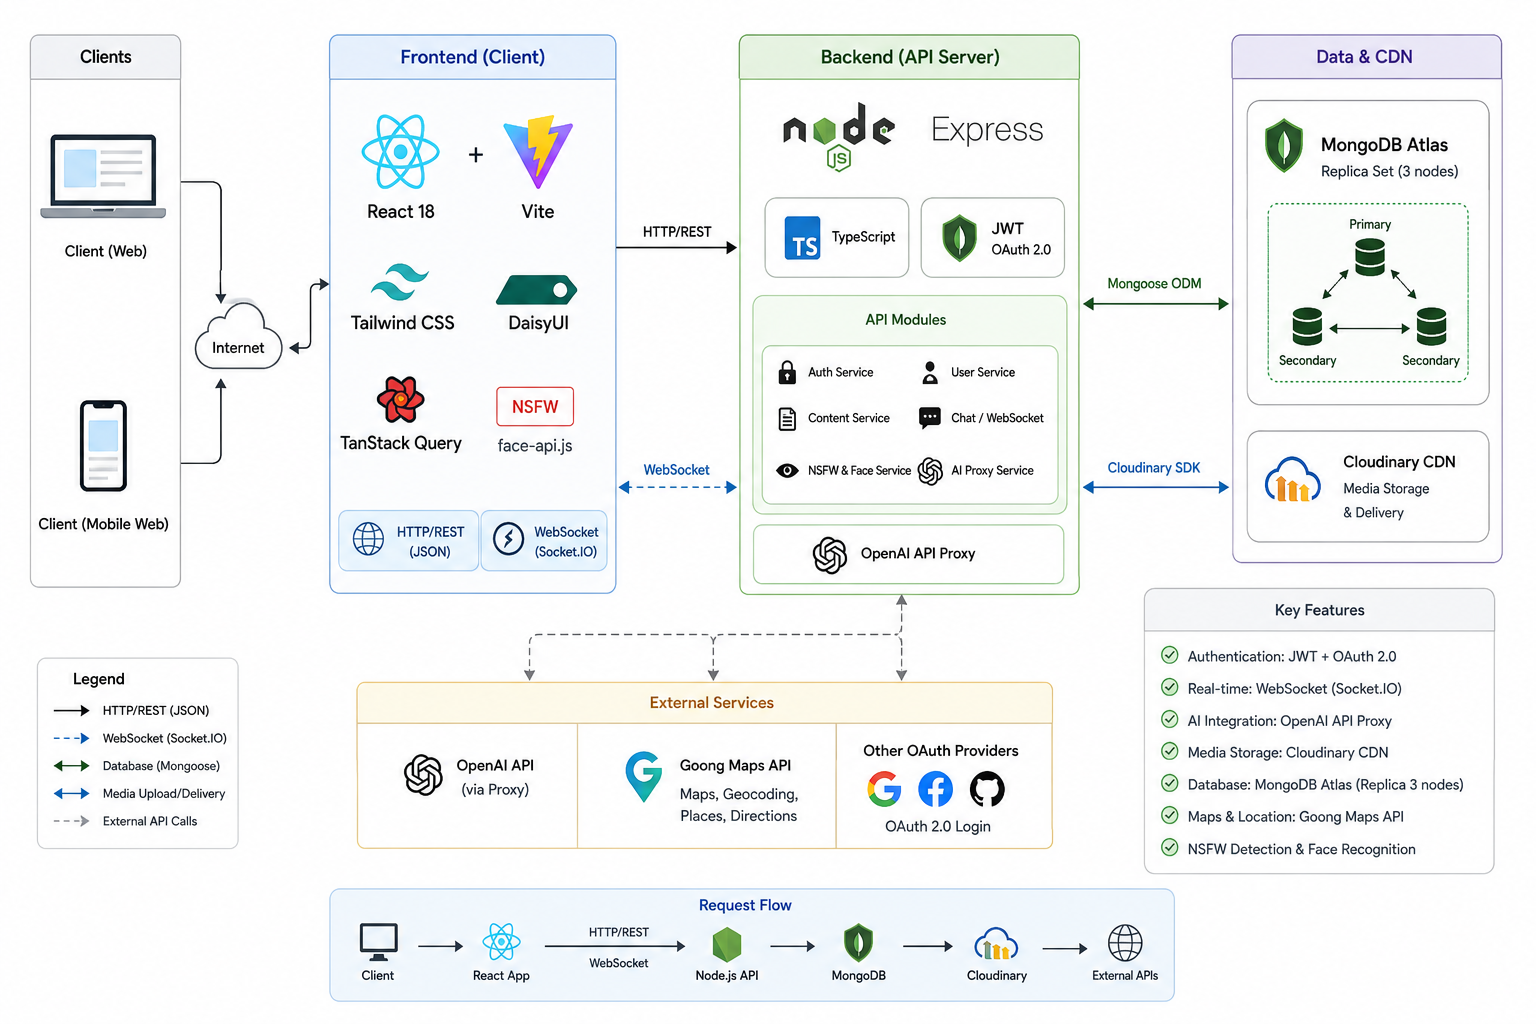
\includegraphics[width=\textwidth]{Images/IMG/Kientruchethong.png}
    \vspace{0.75em}
    \caption{Kiến trúc tổng thể hệ thống: client, Frontend (React/Vite), Backend (Node/Express), tầng dữ liệu (MongoDB, Cloudinary) và dịch vụ ngoài; chú thích luồng HTTP/REST, WebSocket, truy vấn CSDL và upload media.}
    \label{fig:tech_architecture_overview}
\end{figure}

Luồng xử lý điển hình (tham chiếu phần ``Request flow'' trên sơ đồ): \textbf{Client} $\rightarrow$ ứng dụng React $\rightarrow$ (HTTP và/hoặc WebSocket) $\rightarrow$ API Node.js $\rightarrow$ MongoDB và/hoặc Cloudinary $\rightarrow$ gọi API ngoài khi cần.

\section{Công nghệ Frontend và Backend}
\label{sec:tech_frontend}

Bảng~\ref{tab:tech_stack_detail} tóm tắt các công nghệ cốt lõi ở tầng Frontend và Backend, cùng lý do lựa chọn.

\begin{table}[H]
\centering
\caption{Công nghệ Frontend và Backend}
\label{tab:tech_stack_detail}
\small
\renewcommand{\arraystretch}{1.2}
\begin{tabular}{|p{3.2cm}|p{2.5cm}|p{8.3cm}|}
\hline
\textbf{Công nghệ} & \textbf{Lĩnh vực} & \textbf{Mục đích \& Lý do lựa chọn} \\
\hline
\textbf{React.js 18} \cite{ReactJSDocs} & Frontend UI & SPA theo component, hiệu năng tốt; hệ sinh thái TanStack Query, React Hook Form, React Router. \\
\hline
\textbf{TypeScript} \cite{TypeScriptDocs} & Backend (và có thể mở rộng FE) & Kiểu tĩnh, an toàn kiểu, bảo trì dài hạn; Backend hiện thực bằng TypeScript. \\
\hline
\textbf{Tailwind CSS + DaisyUI} & Frontend Styling & Utility-first, bundle gọn, responsive; DaisyUI thống nhất giao diện. \\
\hline
\textbf{Vite} & Build Tool & Khởi động nhanh, HMR, tối ưu bundle production. \\
\hline
\textbf{Node.js + Express.js} \cite{NodeJSDocs,ExpressJSDocs} & Backend API & I/O bất đồng bộ, một ngôn ngữ với Frontend; middleware linh hoạt; tích hợp Socket.IO trên cùng máy chủ HTTP. \\
\hline
\textbf{Socket.IO} & Frontend + Backend & Trừu tượng hóa WebSocket, fallback polling, phù hợp thông báo và tín hiệu thời gian thực. \\
\hline
\end{tabular}
\end{table}

\begin{figure}[H]
   \centering
   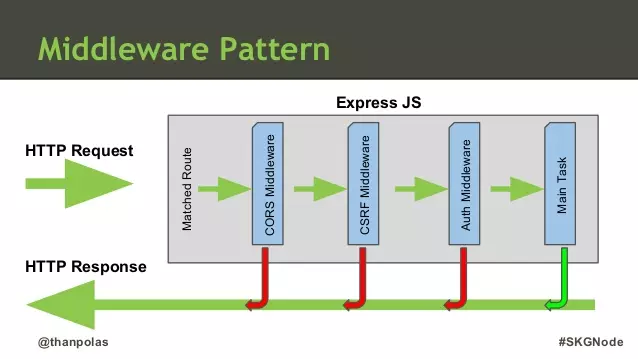
\includegraphics[width=0.65\textwidth]{Images/Middleware.png}
   \vspace{1em}
   \caption{Luồng xử lý request với middleware trong Express.js \cite{VibloMiddleware}}
   \label{fig:expressjs_middleware}
\end{figure}

\section{Cơ sở dữ liệu và dịch vụ bổ trợ}
\label{sec:tech_database}

\subsection{MongoDB và Cloudinary}
\label{subsec:tech_mongodb}

\textbf{MongoDB} \cite{MongoDBDocs} là CSDL NoSQL hướng tài liệu (BSON), phù hợp dữ liệu đa dạng của mạng xã hội thể thao. Mongoose ODM cung cấp schema, validation và truy vấn có cấu trúc. Trên sơ đồ, cụm MongoDB Atlas (replica set) thể hiện mô hình vận hành khuyến nghị khi dùng dịch vụ quản lý; khi tự host trên VPS vẫn giữ cùng vai trò logic trong kiến trúc.

\textbf{Cloudinary} là dịch vụ lưu trữ và phân phối media qua CDN; Backend tích hợp SDK để upload, nhận URL an toàn (HTTPS), giảm tải lưu trữ tĩnh trên VPS.

\begin{figure}[H]
   \centering
   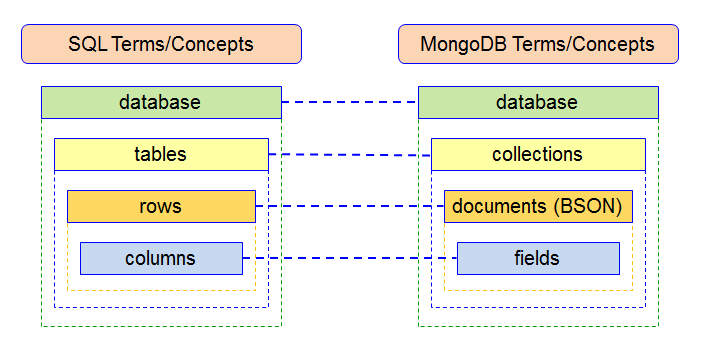
\includegraphics[width=0.65\textwidth]{Images/MongodbandSQL.png}
   \vspace{1em}
   \caption{So sánh cấu trúc dữ liệu MongoDB và SQL}
   \label{fig:mongodb_vs_sql}
\end{figure}

\subsection{Công nghệ triển khai: máy chủ VPS}
\label{subsec:tech_deployment_analysis}

Hệ thống được triển khai trên \textbf{máy chủ VPS} chạy \textbf{Ubuntu}: một máy ảo thuê riêng, tập trung toàn bộ tầng phục vụ ứng dụng (Nginx, tiến trình Node, tùy chọn MongoDB cục bộ). Sơ đồ Hình~\ref{fig:tech_architecture_overview} mô tả \textbf{kiến trúc logic} (thành phần và luồng nghiệp vụ); Hình~\ref{fig:vps_deployment} mô tả \textbf{sơ đồ triển khai VPS}---cách các thành phần đó được bố trí trên một host và điểm ra/vào qua Internet.

\begin{figure}[H]
    \centering
    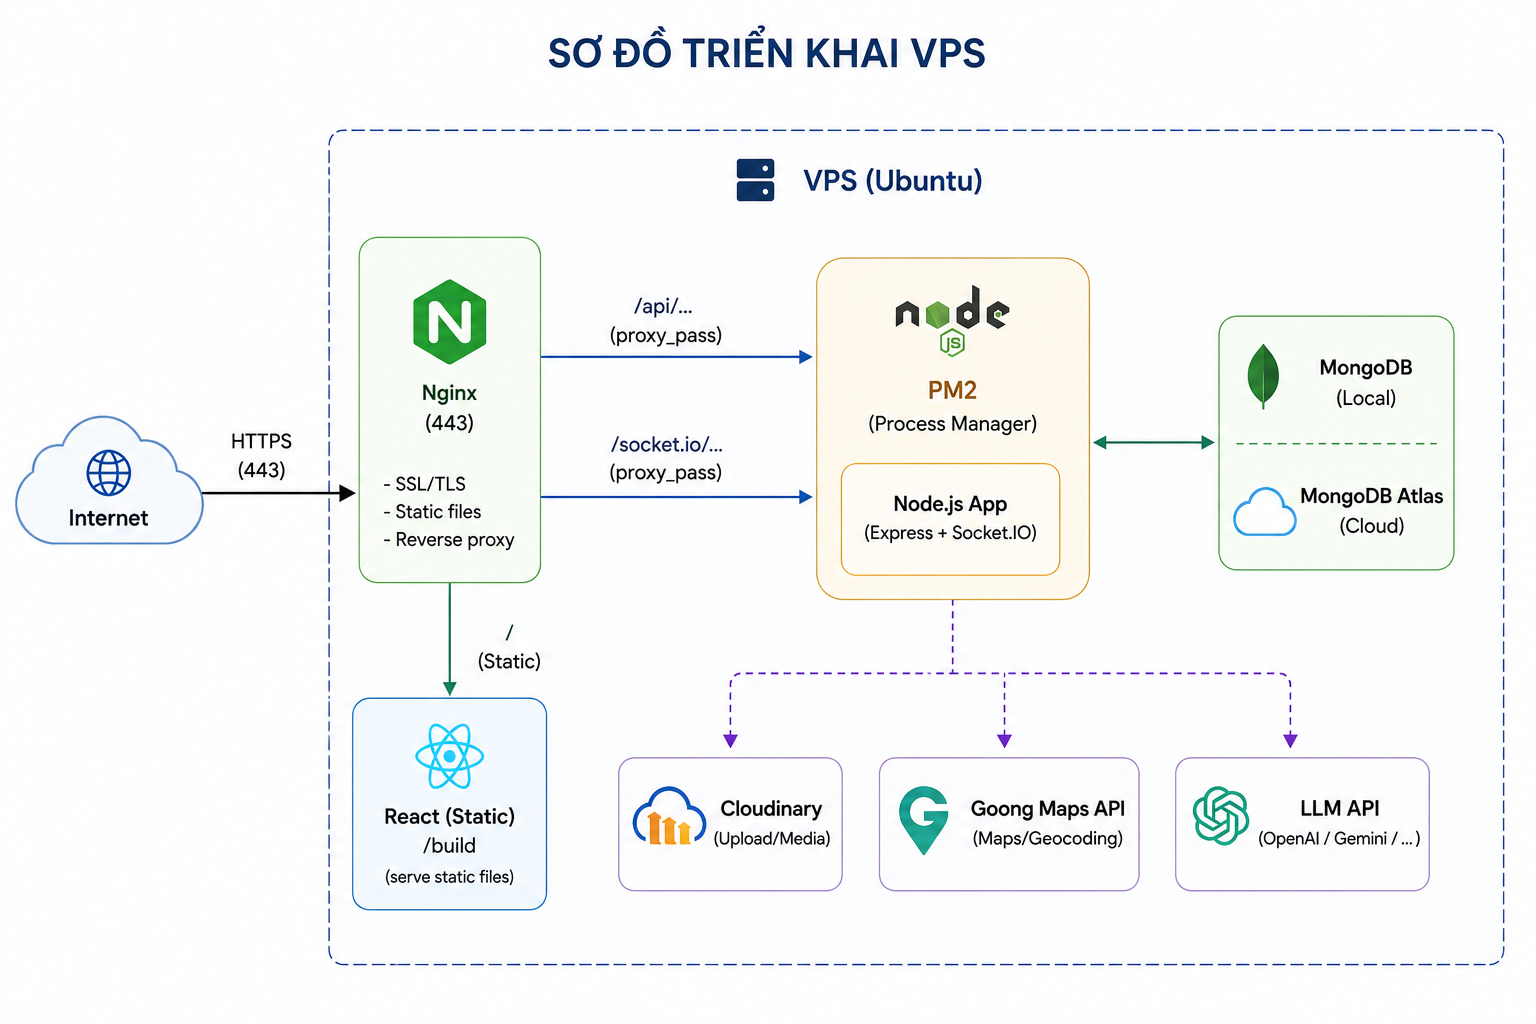
\includegraphics[width=\textwidth]{Images/IMG/deploy.png}
    \vspace{0.75em}
    \caption{Sơ đồ triển khai VPS: truy cập HTTPS, Nginx (TLS, static React, reverse proxy), ứng dụng Node.js (PM2, Express, Socket.IO), MongoDB (local hoặc Atlas), và tích hợp Cloudinary, Goong Maps, API LLM.}
    \label{fig:vps_deployment}
\end{figure}

\subsubsection{Luồng truy cập từ Internet}
Người dùng kết nối qua \textbf{Internet} tới địa chỉ public của VPS. Toàn bộ giao tiếp trình duyệt--máy chủ nên dùng \textbf{HTTPS (cổng 443)}: Nginx chấm dứt TLS (SSL/TLS), phát hành chứng chỉ ví dụ qua Let's Encrypt hoặc chứng chỉ thương mại. HTTPS là cần thiết cho OAuth, bảo vệ token JWT và cookie phiên.

\subsubsection{Nginx: reverse proxy và phục vụ tĩnh}
\textbf{Nginx} đóng vai trò điểm vào duy nhất (\textit{edge}) trước ứng dụng:
\begin{itemize}
    \item \textbf{SSL/TLS:} giải mã HTTPS, có thể bật HTTP/2, header bảo mật cơ bản.
    \item \textbf{React (tĩnh):} thư mục kết quả \texttt{npm run build} của Vite/React được cấu hình làm \textit{root} cho đường dẫn gốc \texttt{/}; Nginx phục vụ HTML/CSS/JS tĩnh, hiệu năng tốt và giảm tải cho Node.
    \item \textbf{Reverse proxy tới Node:} các yêu cầu có tiền tố \texttt{/api/...} được chuyển tiếp tới tiến trình Backend (REST JSON). Các yêu cầu \texttt{/socket.io/...} (và nâng cấp WebSocket tương thích Socket.IO) cũng được proxy tới cùng ứng dụng Node để thông báo, phòng gọi video và tín hiệu thời gian thực hoạt động đúng sau một cổng/domain thống nhất.
\end{itemize}
Cấu hình \texttt{proxy\_http\_version 1.1}, \texttt{Upgrade}, \texttt{Connection} cho đoạn WebSocket là thông lệ khi ghép Nginx với Socket.IO.

\subsubsection{Backend: Node.js, Express, Socket.IO và PM2}
Ứng dụng \textbf{Node.js} (Express, TypeScript sau biên dịch) lắng nghe cổng nội bộ (ví dụ \texttt{127.0.0.1:4000}), không expose trực tiếp ra Internet. \textbf{PM2} (hoặc \textbf{systemd}) giữ tiến trình sống, tự khởi động lại khi crash hoặc khi reboot VPS, ghi log tập trung---phù hợp vận hành production trên một máy. Một tiến trình duy nhất phục vụ cả REST và Socket.IO trên cùng HTTP server (mô hình MERN-style đã dùng trong dự án).

\subsubsection{Cơ sở dữ liệu trên VPS hoặc cloud}
Sơ đồ thể hiện hai hướng tương thích:
\begin{itemize}
    \item \textbf{MongoDB (local):} cài trực tiếp trên VPS, giảm độ trễ nội bộ và chi phí cluster; cần sao lưu, cập nhật bản vá và giới hạn tài nguyên RAM/đĩa.
    \item \textbf{MongoDB Atlas:} CSDL trên đám mây, VPS chỉ chạy ứng dụng; phù hợp khi muốn replica, backup và bảo trì do nhà cung cấp đảm nhiệm.
\end{itemize}
Ứng dụng chỉ cần chuỗi kết nối \texttt{MONGODB\_URL} phù hợp; Mongoose giữ nguyên vai trò ODM trong cả hai trường hợp.

\subsubsection{Dịch vụ bên thứ ba (ngoài VPS)}
Backend gọi ra Internet tới các API không nằm trên VPS:
\begin{itemize}
    \item \textbf{Cloudinary}---upload, lưu trữ và CDN cho ảnh/video.
    \item \textbf{Goong Maps API}---bản đồ, địa lý, tuyến đường (phía client dùng SDK/map tiles; server có thể dùng khi cần).
    \item \textbf{LLM API}---các nhà cung cấp như OpenAI, Gemini hoặc endpoint tương thích OpenAI (trong mã nguồn hiện tại có tích hợp kiểu OpenAI-compatible, ví dụ Groq) cho tính năng gợi ý, kiểm tra nội dung, v.v.
\end{itemize}
Các khóa API được đặt trong biến môi trường trên VPS, không đưa vào mã nguồn.

\subsubsection{Tùy chọn: Docker và email AWS SES}
\textbf{Docker} \cite{DockerDocs} (Hình~\ref{fig:docker_architecture}) có thể đóng gói Backend hoặc toàn stack để đồng nhất môi trường; trên VPS production vẫn thường cần Nginx phía trước container (hoặc tương đương) cho TLS và tĩnh. \textbf{AWS SES} có thể dùng để gửi email hệ thống, độc lập với việc ứng dụng chạy trên VPS (không bắt buộc EC2/CloudFront).

\begin{figure}[H]
   \centering
   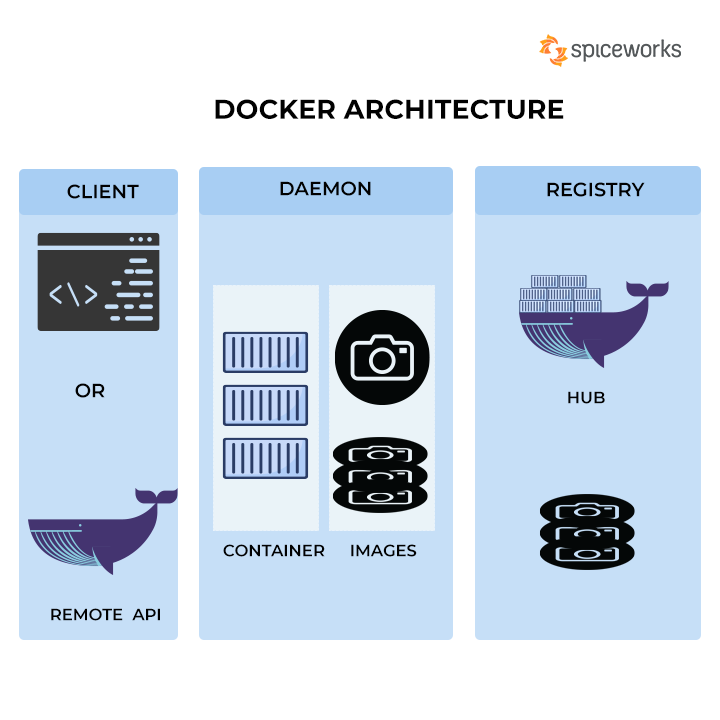
\includegraphics[width=0.7\textwidth]{Images/Docker-Architecture.png}
   \vspace{1em}
   \caption{Kiến trúc Docker \cite{DockerDocs} (công cụ đóng gói tùy chọn khi triển khai)}
   \label{fig:docker_architecture}
\end{figure}

\section{Kết luận}
\label{sec:tech_conclusion}

Stack và kiến trúc được chọn theo các tiêu chí: đáp ứng chức năng mạng xã hội thể thao, hiệu năng tốt, khả năng mở rộng, cộng đồng lớn và tốc độ phát triển. React + Vite + Tailwind/DaisyUI xây dựng giao diện hiện đại; Node.js + Express + TypeScript phục vụ REST và Socket.IO; MongoDB + Mongoose lưu trữ linh hoạt; Cloudinary đảm nhiệm media; tích hợp LLM (API kiểu OpenAI), Goong Maps và OAuth bổ sung năng lực thông minh và bản đồ. Triển khai thực tế trên \textbf{VPS Ubuntu} (Hình~\ref{fig:vps_deployment}) dùng Nginx (HTTPS, static build, proxy \texttt{/api} và \texttt{/socket.io}), PM2 cho Node, MongoDB local hoặc Atlas, và các API ngoài cho media, bản đồ và LLM. Thiết kế chi tiết use case và thành phần hệ thống được trình bày tại Chương~\ref{chap:system_design}.

\textbf{Hướng phát triển:} Redis cache, hàng đợi message, CI/CD, giám sát (Prometheus/Grafana), mở rộng đa máy chủ hoặc tách tier khi tải tăng.


\chapter{HIỆN THỰC HỆ THỐNG}
\renewcommand*{\theHsection}{\theHchapter.\the\value{section}}
\label{chap:implementation}

Chương này trình bày chi tiết quá trình hiện thực hệ thống nền tảng mạng xã hội thể thao cộng đồng FitConnect, bao gồm môi trường và công cụ phát triển, cấu trúc tổ chức mã nguồn, và từng nhóm tính năng đã được triển khai đầy đủ. Với mỗi nhóm tính năng, nội dung trình bày theo ba lớp: mô tả chức năng, luồng xử lý kỹ thuật và giao diện thực tế từ hệ thống.

% ==================================================
\section{Môi trường phát triển}
\label{sec:impl_dev_environment}
% ==================================================

\subsection{Nền tảng và ngôn ngữ lập trình}
\label{subsec:impl_platform}

Toàn bộ hệ thống FitConnect được phát triển trên nền tảng \textbf{JavaScript/TypeScript} xuyên suốt từ Frontend đến Backend, đảm bảo tính đồng nhất về ngôn ngữ và khả năng tái sử dụng logic nghiệp vụ. Quyết định sử dụng TypeScript (thay vì JavaScript thuần) được đưa ra ngay từ đầu để tận dụng hệ thống kiểu tĩnh, giúp phát hiện lỗi tại thời điểm biên dịch, cải thiện khả năng bảo trì và nâng cao chất lượng mã nguồn ở quy mô lớn.

\begin{table}[H]
\centering
\caption{Nền tảng và ngôn ngữ sử dụng trong hệ thống FitConnect}
\label{tab:impl_platform}
\begin{tabular}{|p{4cm}|p{4cm}|p{6cm}|}
\hline
\textbf{Thành phần} & \textbf{Nền tảng / Ngôn ngữ} & \textbf{Phiên bản} \\
\hline
Runtime Backend & Node.js & v20.19.4 (LTS) \\
\hline
Ngôn ngữ & TypeScript & 5.x \\
\hline
Package Manager & npm & 10.x \\
\hline
Build Tool (FE) & Vite & 5.x \\
\hline
Hệ điều hành phát triển & Windows 11 & --- \\
\hline
\end{tabular}
\end{table}

Node.js phiên bản 20 LTS được chọn vì đây là phiên bản ổn định dài hạn (Long-Term Support) với hiệu năng V8 Engine tối ưu, hỗ trợ đầy đủ ES Modules và các API bất đồng bộ hiện đại. Vite được ưu tiên thay cho Create React App truyền thống nhờ tốc độ khởi động dev server gần như tức thời thông qua cơ chế Hot Module Replacement (HMR) dựa trên native ESM.

\subsection{Công cụ và phần mềm hỗ trợ}
\label{subsec:impl_tools}

\begin{table}[H]
\centering
\caption{Công cụ phát triển sử dụng trong dự án FitConnect}
\label{tab:impl_tools}
\begin{tabular}{|p{3.5cm}|p{3.5cm}|p{7cm}|}
\hline
\textbf{Nhóm} & \textbf{Công cụ} & \textbf{Mục đích sử dụng} \\
\hline
\textbf{IDE / Editor} & Visual Studio Code & Môi trường lập trình chính với hỗ trợ TypeScript, IntelliSense, debug tích hợp \\
\hline
\textbf{Extension VS Code} & ESLint, Prettier, GitLens, Tailwind CSS IntelliSense & Kiểm tra lỗi cú pháp, định dạng code tự động, quản lý lịch sử Git, gợi ý class Tailwind \\
\hline
\textbf{Quản lý phiên bản} & Git \& GitHub & Kiểm soát mã nguồn, branching, code review, lưu trữ từ xa \\
\hline
\textbf{Kiểm thử API} & Postman & Thiết kế, kiểm thử và tài liệu hóa toàn bộ REST API endpoint \\
\hline
\textbf{Quản lý CSDL} & MongoDB Compass & Giao diện đồ họa để truy vấn, kiểm tra dữ liệu và tối ưu index trong MongoDB \\
\hline
\textbf{Quản lý biến môi trường} & .env + dotenv & Tách biệt cấu hình nhạy cảm (API key, chuỗi kết nối DB) khỏi mã nguồn \\
\hline
\textbf{Lưu trữ media} & AWS S3 (SDK v3) + Cloudinary & Lưu trữ ảnh/video; Cloudinary xử lý biến đổi ảnh tự động (resize, optimize) \\
\hline
\textbf{Gửi email} & AWS SES + Nodemailer & Gửi email xác thực, khôi phục mật khẩu và thông báo hệ thống \\
\hline
\end{tabular}
\end{table}

\subsection{Các thư viện và framework chính}
\label{subsec:impl_libraries}

\subsubsection{Frontend (DATN\_FE)}
\label{subsubsec:impl_fe_libs}

Frontend được xây dựng trên nền tảng \textbf{React 18} kết hợp \textbf{TypeScript}, tận dụng các tính năng mới nhất như Concurrent Rendering và Automatic Batching. Bảng dưới liệt kê các thư viện cốt lõi và lý do lựa chọn:

\begin{table}[H]
\centering
\caption{Thư viện Frontend chính của hệ thống FitConnect}
\label{tab:impl_fe_libs}
\begin{tabular}{|p{4.5cm}|p{2cm}|p{7.5cm}|}
\hline
\textbf{Thư viện} & \textbf{Phiên bản} & \textbf{Vai trò} \\
\hline
React & 18.2 & Thư viện xây dựng giao diện người dùng, quản lý component lifecycle \\
\hline
React Router DOM & 6.16 & Điều hướng trang (SPA routing), protected routes phân quyền \\
\hline
TanStack React Query & 5.28 & Quản lý trạng thái dữ liệu server: caching, background sync, infinite scroll \\
\hline
React Hook Form + Yup & 7.51 / 1.4 & Quản lý form hiệu năng cao, validation schema khai báo theo chuẩn \\
\hline
Tailwind CSS + DaisyUI & 3.x & Styling utility-first, design system nhất quán, responsive layout \\
\hline
Socket.io-client & 4.7.5 & Kết nối WebSocket hai chiều cho thông báo và sự kiện thời gian thực \\
\hline
React Leaflet / Goong Maps & 5.0 / 1.0.9 & Hiển thị bản đồ, vẽ lộ trình GPS cho tính năng sự kiện ngoài trời \\
\hline
Recharts / Chart.js & 2.15 & Vẽ biểu đồ thống kê sức khỏe, tiến độ sự kiện và thử thách \\
\hline
React Body Highlighter & 2.0.5 & Trực quan hóa nhóm cơ bắp khi xây dựng giáo án tập luyện \\
\hline
React Quill & 2.0 & Rich text editor cho tính năng đăng bài viết và blog \\
\hline
Axios & 1.x & HTTP client với interceptor tự động gắn JWT token vào mỗi request \\
\hline
\end{tabular}
\end{table}

\subsubsection{Backend (DATN\_BE)}
\label{subsubsec:impl_be_libs}

Backend được xây dựng theo kiến trúc \textbf{RESTful API} với \textbf{Express.js} và \textbf{TypeScript}, tổ chức code theo mô hình Controller -- Service -- Model để tách biệt rõ ràng các lớp nghiệp vụ:

\begin{table}[H]
\centering
\caption{Thư viện Backend chính của hệ thống FitConnect}
\label{tab:impl_be_libs}
\begin{tabular}{|p{4.5cm}|p{2cm}|p{7.5cm}|}
\hline
\textbf{Thư viện} & \textbf{Phiên bản} & \textbf{Vai trò} \\
\hline
Express.js & 4.18.2 & Framework HTTP server, định nghĩa router, middleware pipeline \\
\hline
Mongoose & 8.0 & ODM (Object Document Mapper) cho MongoDB, định nghĩa schema và thực hiện truy vấn \\
\hline
Socket.io & 4.7.5 & WebSocket server xử lý thông báo real-time, phòng Video Call \\
\hline
JSON Web Token & 9.0.2 & Phát hành và xác thực Access Token / Refresh Token \\
\hline
Bcrypt & 5.1.1 & Mã hóa một chiều (hash + salt) mật khẩu người dùng \\
\hline
Multer + Sharp & 1.4.5 / 0.33.5 & Xử lý upload file, nén và chuyển đổi định dạng ảnh trước khi lưu \\
\hline
Cloudinary SDK & 2.9 & Upload ảnh/video lên CDN, tự động tối ưu theo thiết bị \\
\hline
AWS SDK v3 (S3, SES) & 3.540 & Lưu trữ file trên S3, gửi email transactional qua SES \\
\hline
Express Validator & 7.0.1 & Validate và sanitize dữ liệu đầu vào từ client \\
\hline
Express Rate Limit & 6.11 & Giới hạn số request mỗi IP, chống tấn công brute-force \\
\hline
Helmet & 7.0 & Bảo mật HTTP headers (XSS, Clickjacking, MIME sniffing) \\
\hline
Morgan & 1.10 & Ghi log HTTP request/response trong quá trình phát triển \\
\hline
Nodemailer & 6.9.13 & Gửi email xác thực và thông báo thông qua SMTP / AWS SES \\
\hline
Moment Timezone & 0.5.45 & Chuẩn hóa và tính toán thời gian đa múi giờ cho sự kiện và thử thách \\
\hline
\end{tabular}
\end{table}

\subsection{Cấu trúc tổ chức dự án}
\label{subsec:impl_project_structure}

Dự án được tổ chức theo mô hình \textbf{monorepo} với ba thư mục ứng dụng hoàn toàn độc lập, mỗi thư mục đảm nhiệm một vai trò riêng biệt trong hệ sinh thái:

\begin{table}[H]
\centering
\caption{Cấu trúc monorepo dự án FitConnect}
\label{tab:impl_monorepo}
\begin{tabular}{|p{3.5cm}|p{4.5cm}|p{6cm}|}
\hline
\textbf{Thư mục} & \textbf{Stack công nghệ} & \textbf{Vai trò} \\
\hline
\texttt{DATN\_FE/} & React 18 + TypeScript + Vite & Giao diện người dùng cuối (User Frontend) \\
\hline
\texttt{DATN\_BE/} & Node.js + Express + TypeScript + MongoDB & API Server và xử lý nghiệp vụ (Backend) \\
\hline
\texttt{DATN\_ADMIN\_FE/} & React 18 + JavaScript + Vite & Giao diện quản trị viên (Admin Frontend) \\
\hline
\end{tabular}
\end{table}

Việc tách biệt thành ba ứng dụng riêng biệt giúp Frontend người dùng và Admin Frontend triển khai lên các miền khác nhau với cấu hình CORS độc lập, trong khi Backend đóng vai trò API duy nhất phục vụ cả hai client. Admin Frontend (\texttt{DATN\_ADMIN\_FE}) gồm 10 trang tập trung vào giám sát và kiểm duyệt: Dashboard, quản lý người dùng, báo cáo vi phạm, sự kiện, thử thách, danh mục thể thao, kho bài tập và quản lý kiểm duyệt viên.

\subsubsection{Cấu trúc thư mục Frontend người dùng (DATN\_FE)}
\label{subsubsec:impl_frontend_structure}

Frontend người dùng gồm hơn 54 trang, được tổ chức theo nhóm tính năng để dễ bảo trì và mở rộng:

\begin{lstlisting}[basicstyle=\ttfamily\small, frame=single, breaklines=true]
DATN_FE/src/
|-- components/      # Component tai su dung toan cuc (Button, Modal, Card...)
|-- pages/           # 54 trang tuong ung cac tinh nang he thong
|   |-- Home/        # Bang tin cong dong (Newsfeed)
|   |-- SportEvent/  # Su kien the thao (tao, tham gia, GPS, Video Call)
|   |-- Challenge/   # Thu thach cong dong (check-in, bang xep hang)
|   |-- Training/    # Tap luyen ca nhan (giao an, AI goi y)
|   |-- Calculator/  # Bo cong cu tinh chi so suc khoe
|   |-- Calendar/    # Lich ca nhan va thong bao
|   |-- Me/          # Ho so va dashboard ca nhan
|   |-- Friends/     # Ket noi ban be, theo doi
|   `-- Auth/        # Dang ky, dang nhap, quen mat khau
|-- services/        # Tang goi API (axios instances, endpoints)
|-- hooks/           # Custom React hooks (useAuth, useSocket...)
|-- utils/           # Ham tien ich (format date, tinh BMI, TDEE...)
|-- contexts/        # React Context (AuthContext, SocketContext)
|-- types/           # TypeScript interface va type definitions
`-- App.tsx          # Root component va cau hinh routes
\end{lstlisting}

\subsubsection{Cấu trúc thư mục Backend hệ thống (DATN\_BE)}
\label{subsubsec:impl_backend_structure}

Backend triển khai kiến trúc ba lớp \textbf{Routes~$\rightarrow$~Controllers~$\rightarrow$~Services}, đảm bảo nguyên tắc Single Responsibility --- mỗi lớp chỉ đảm nhận đúng một trách nhiệm:

\begin{lstlisting}[basicstyle=\ttfamily\small, frame=single, breaklines=true]
DATN_BE/src/
|-- routes/
|   |-- userRoutes/        # 30 nhom route danh cho nguoi dung
|   `-- adminRoutes/       # 10 nhom route danh cho quan tri vien
|-- controllers/           # Nhan request, goi service, tra response
|-- services/              # Toan bo business logic nghiep vu
|-- models/                # Mongoose schemas (9 collection chinh)
|-- middlewares/           # accessTokenValidator, checkRole, upload...
|-- utils/                 # sendEmail, handleError, hashPassword...
|-- config/                # Cau hinh DB, environment variables
`-- index.ts               # Entry point, khoi dong server & Socket.io
\end{lstlisting}

Routes chỉ khai báo endpoint và middleware, Controllers điều phối luồng dữ liệu, Services chứa toàn bộ logic nghiệp vụ. Cách tổ chức này giúp kiểm thử từng lớp độc lập và dễ dàng mở rộng khi bổ sung tính năng mới.

\subsubsection{Cấu trúc tổ chức cơ sở dữ liệu}
\label{subsubsec:impl_db_structure}

Hệ thống sử dụng \textbf{MongoDB} --- cơ sở dữ liệu NoSQL hướng tài liệu --- được quản lý thông qua \textbf{Mongoose ODM}. Toàn bộ dữ liệu được tổ chức thành \textbf{9 nhóm collection} tương ứng với 9 nhóm tính năng của nền tảng:

\begin{table}[H]
\centering
\caption{Cấu trúc cơ sở dữ liệu hệ thống FitConnect}
\label{tab:impl_db_structure}
\begin{tabular}{|p{0.8cm}|p{3.8cm}|>{\raggedright\arraybackslash}p{9.4cm}|}
\hline
\textbf{STT} & \textbf{Nhóm collection} & \textbf{Các collection thuộc nhóm} \\
\hline
1 & Tài khoản người dùng & users, follows, notifications \\
\hline
2 & Nội dung cộng đồng & posts, imagePost, commentPost, likePost \\
\hline
3 & Sự kiện thể thao & sportEvents, sportEventParticipants, sportEventActivities, sportEventDayComments \\
\hline
4 & Thử thách cộng đồng & challenges, challengeParticipants, challengeProgress, challengeDayComments \\
\hline
5 & Tập luyện cá nhân & exercises, workoutSessions, workoutSchedules, savedWorkoutTemplates, equipment, muscleGroups \\
\hline
6 & Sức khỏe cá nhân & healthMetrics, activityTracking, activities \\
\hline
7 & Thể thao ngoài trời & userCalendars \\
\hline
8 & AI và theo dõi sử dụng & aiUsageLogs \\
\hline
9 & Quản trị hệ thống & sportCategories, reports \\
\hline
\end{tabular}
\end{table}

Mỗi collection được định nghĩa với schema chặt chẽ thông qua Mongoose, bao gồm kiểu dữ liệu, ràng buộc (required, unique, enum), quan hệ tham chiếu qua ObjectId và các index tối ưu cho truy vấn thường xuyên. Thiết kế schema theo mô hình embedding cho dữ liệu ít thay đổi (ví dụ: mảng thành viên sự kiện) và mô hình referencing cho dữ liệu có vòng đời độc lập (ví dụ: người dùng, bài tập), đảm bảo hiệu suất truy vấn tối ưu trong từng tình huống.

% ==================================================
\section{Ứng dụng trí tuệ nhân tạo và xử lý thông minh}
\label{sec:impl_ai_smart}
% ==================================================

Hệ thống FitConnect tích hợp trí tuệ nhân tạo (AI) xuyên suốt nhiều nhóm tính năng nhằm nâng cao trải nghiệm người dùng, tự động hóa các thao tác phức tạp, và đảm bảo chất lượng nội dung cộng đồng. AI trong hệ thống được chia thành ba nhóm chính: \textbf{Nhận diện và kiểm soát nội dung} (xử lý ảnh nhạy cảm, lọc từ ngữ nhạy cảm trong bài viết và bình luận, xác minh ảnh bữa ăn, nhận diện khuôn mặt), \textbf{Tạo nội dung tự động} (AI điền tự động sự kiện, thử thách), và \textbf{Phân tích và gợi ý cá nhân hóa} (phân tích sức khỏe, gợi ý bài tập).

\subsection{Nhận diện và kiểm soát nội dung hình ảnh}
\label{subsec:impl_ai_content_control}

\subsubsection{Kiểm tra ảnh nhạy cảm khi đăng bài cộng đồng}

Khi người dùng đính kèm hình ảnh vào bài viết, hệ thống tự động quét ảnh ngay trên trình duyệt bằng mô hình NSFW Detection chạy trên TensorFlow.js (client-side, không cần gửi lên server). Nếu ảnh vượt ngưỡng xác suất nhạy cảm cho phép, hệ thống chặn đăng bài và hiển thị cảnh báo ngay lập tức.

\begin{figure}[H]
    \centering
    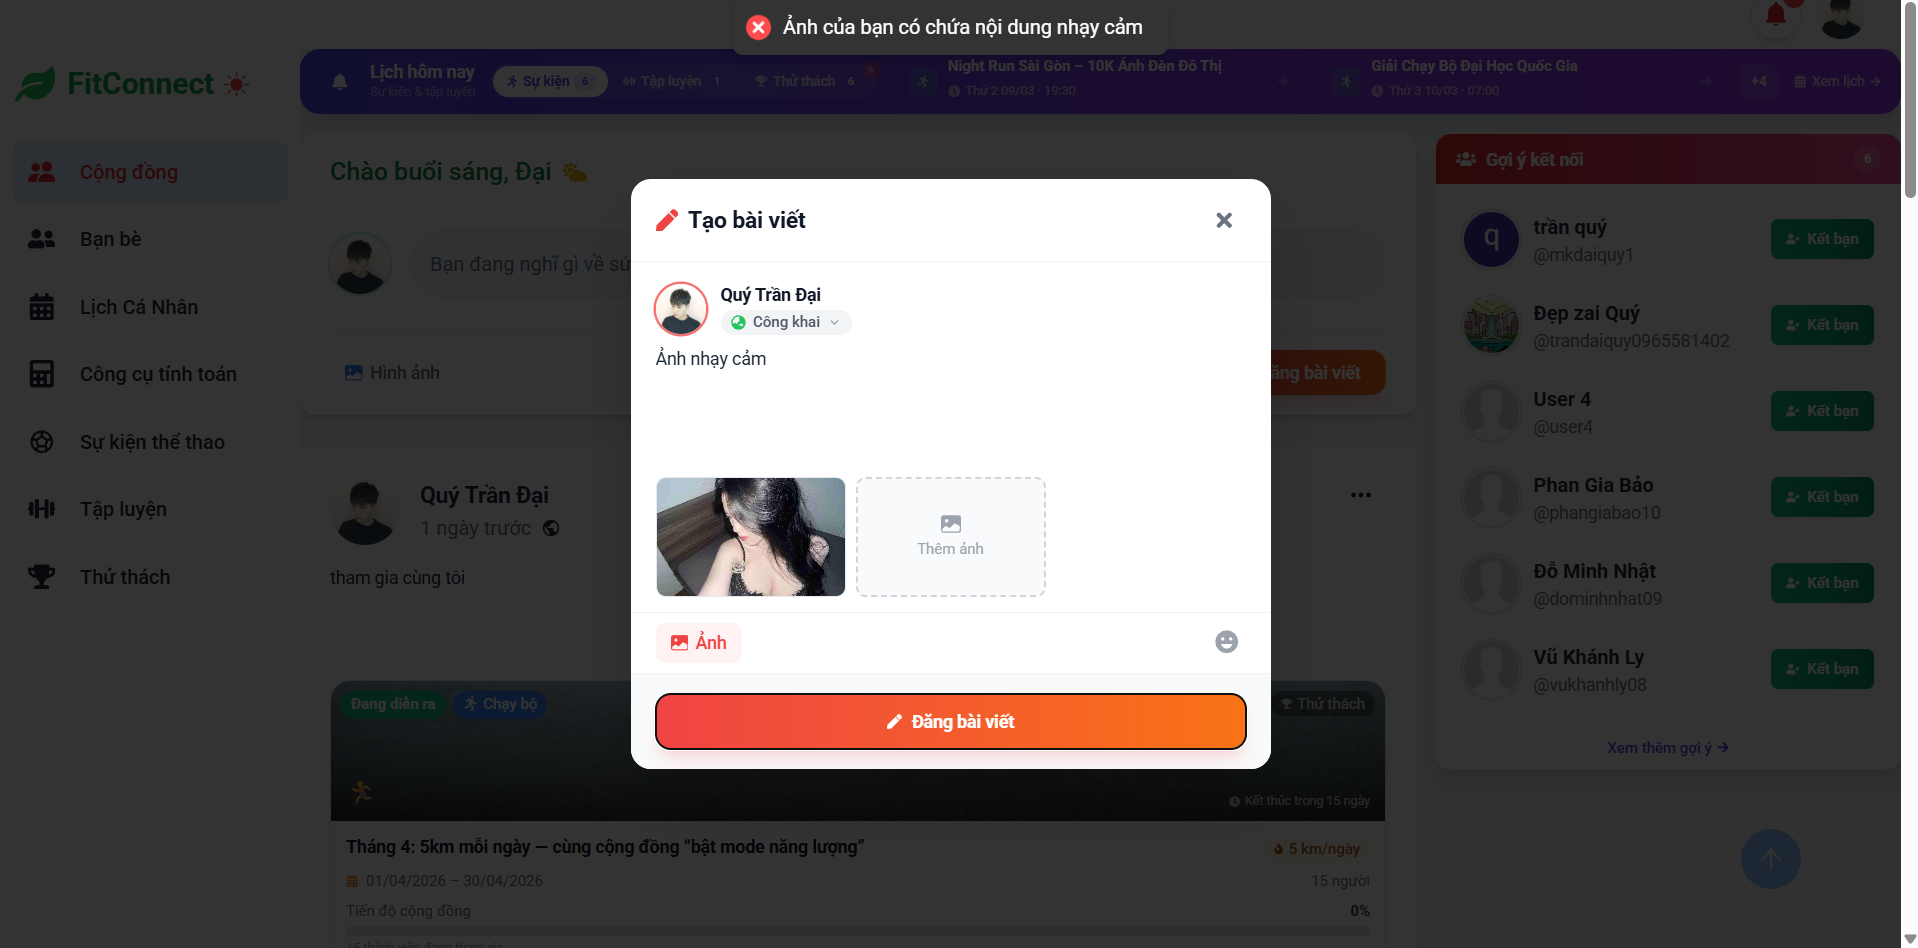
\includegraphics[width=0.60\textwidth]{Images/IMG/CongDong/AInhanbietanhnhaycam.png}
    \caption{Hệ thống AI phát hiện và cảnh báo ảnh nhạy cảm khi người dùng đăng bài}
    \label{fig:impl_ai_nsfw}
\end{figure}

\subsubsection{Lọc từ ngữ nhạy cảm khi đăng bài và bình luận}

Khi người dùng soạn bài viết hoặc gửi bình luận, hệ thống tự động phân tích văn bản bằng mô hình lọc ngôn ngữ theo quy tắc (rule-based). Nếu phát hiện từ hoặc cụm từ vi phạm, hệ thống chặn hành động và hiển thị thông báo lỗi ngay lập tức, ngăn nội dung không phù hợp được đăng lên cộng đồng. Cơ chế áp dụng đồng nhất cho cả bài viết lẫn bình luận.

\begin{figure}[H]
    \centering
    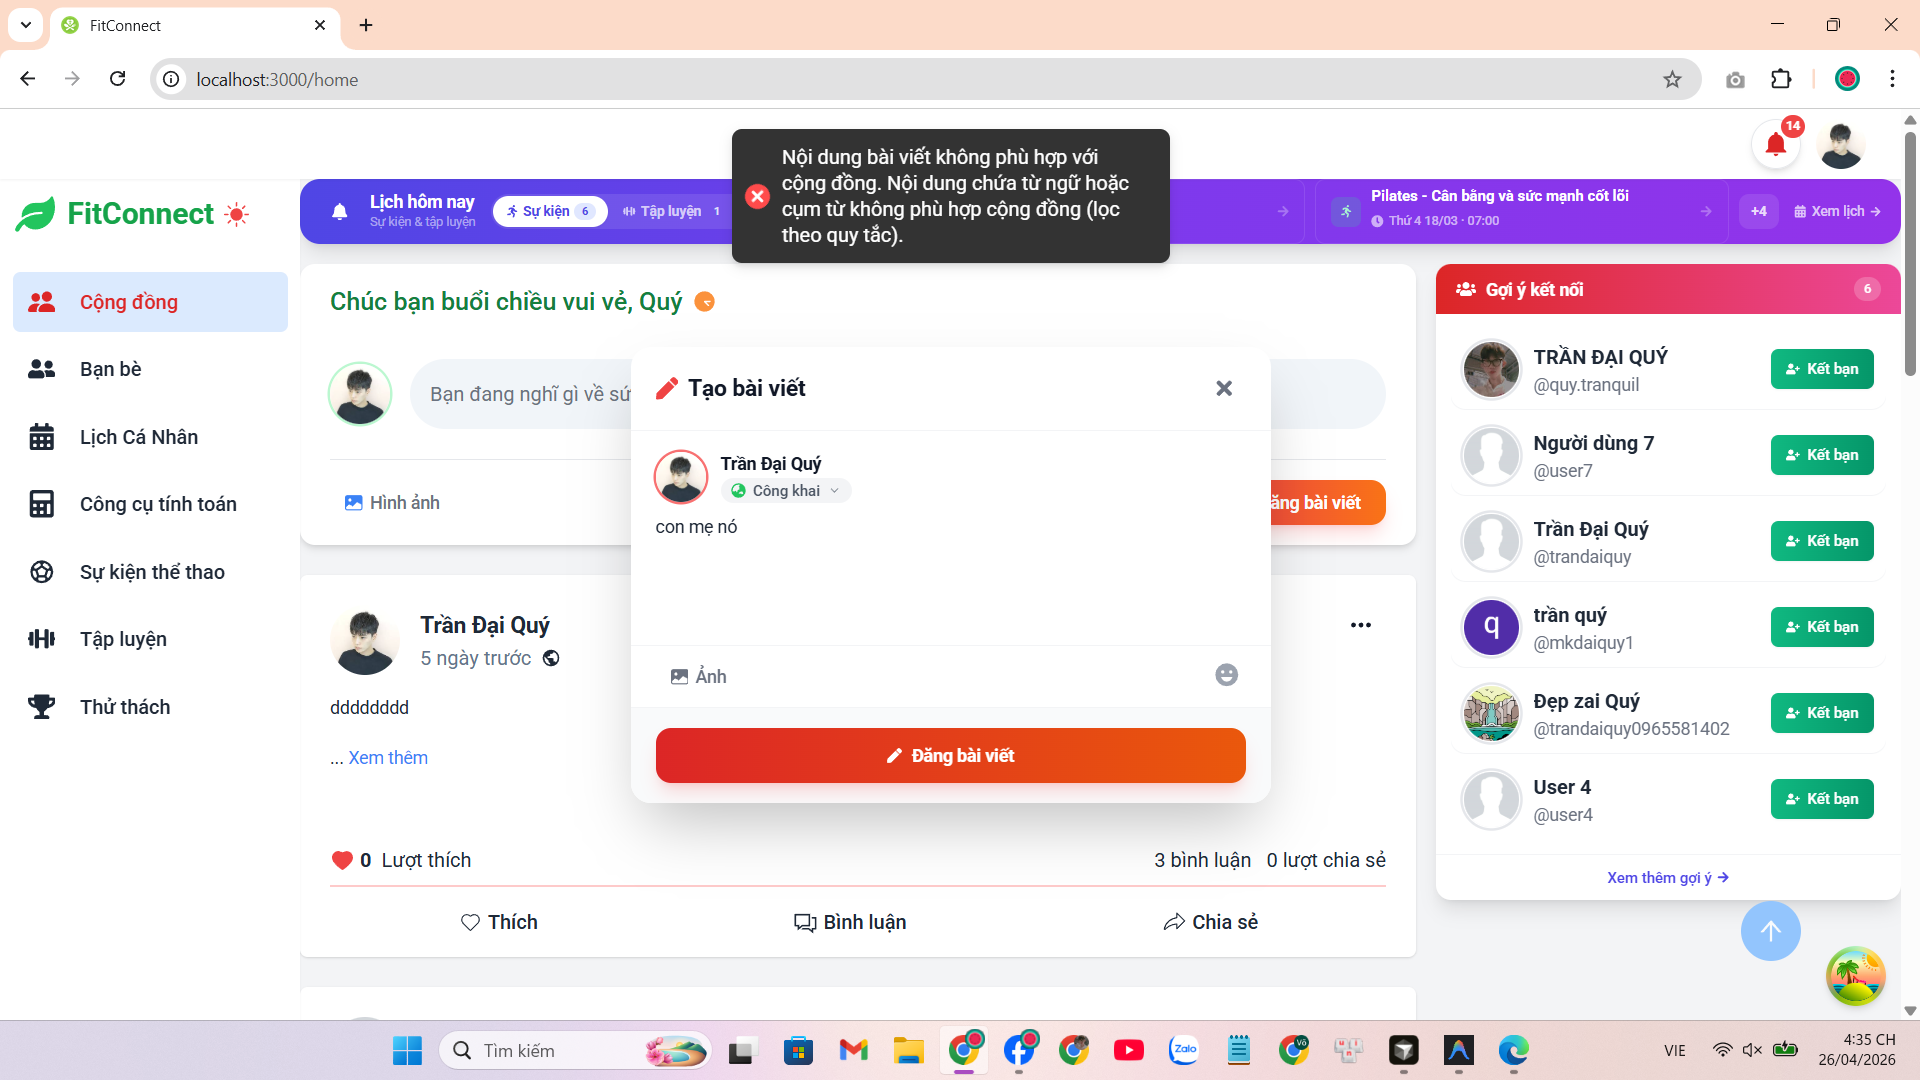
\includegraphics[width=0.60\textwidth]{Images/IMG/Nhom2/dangbainoidungnhaycam.png}
    \caption{Hệ thống phát hiện và chặn đăng bài viết chứa từ ngữ không phù hợp}
    \label{fig:impl_ai_post_filter}
\end{figure}

\subsubsection{Nhận diện khuôn mặt trong phiên Video Call sự kiện trong nhà}

Trong sự kiện thể thao trong nhà, hệ thống dùng TinyFaceDetector (face-api.js) chạy trực tiếp trên trình duyệt để theo dõi sự hiện diện của người tham gia trước camera. Khi phát hiện khuôn mặt, hệ thống hiển thị badge xanh ``AI đang theo dõi'' và tích lũy thời gian tham gia thực tế; khi người dùng rời camera quá lâu, đồng hồ tự dừng và hiển thị trạng thái ``Vắng''.

\begin{figure}[H]
    \centering
    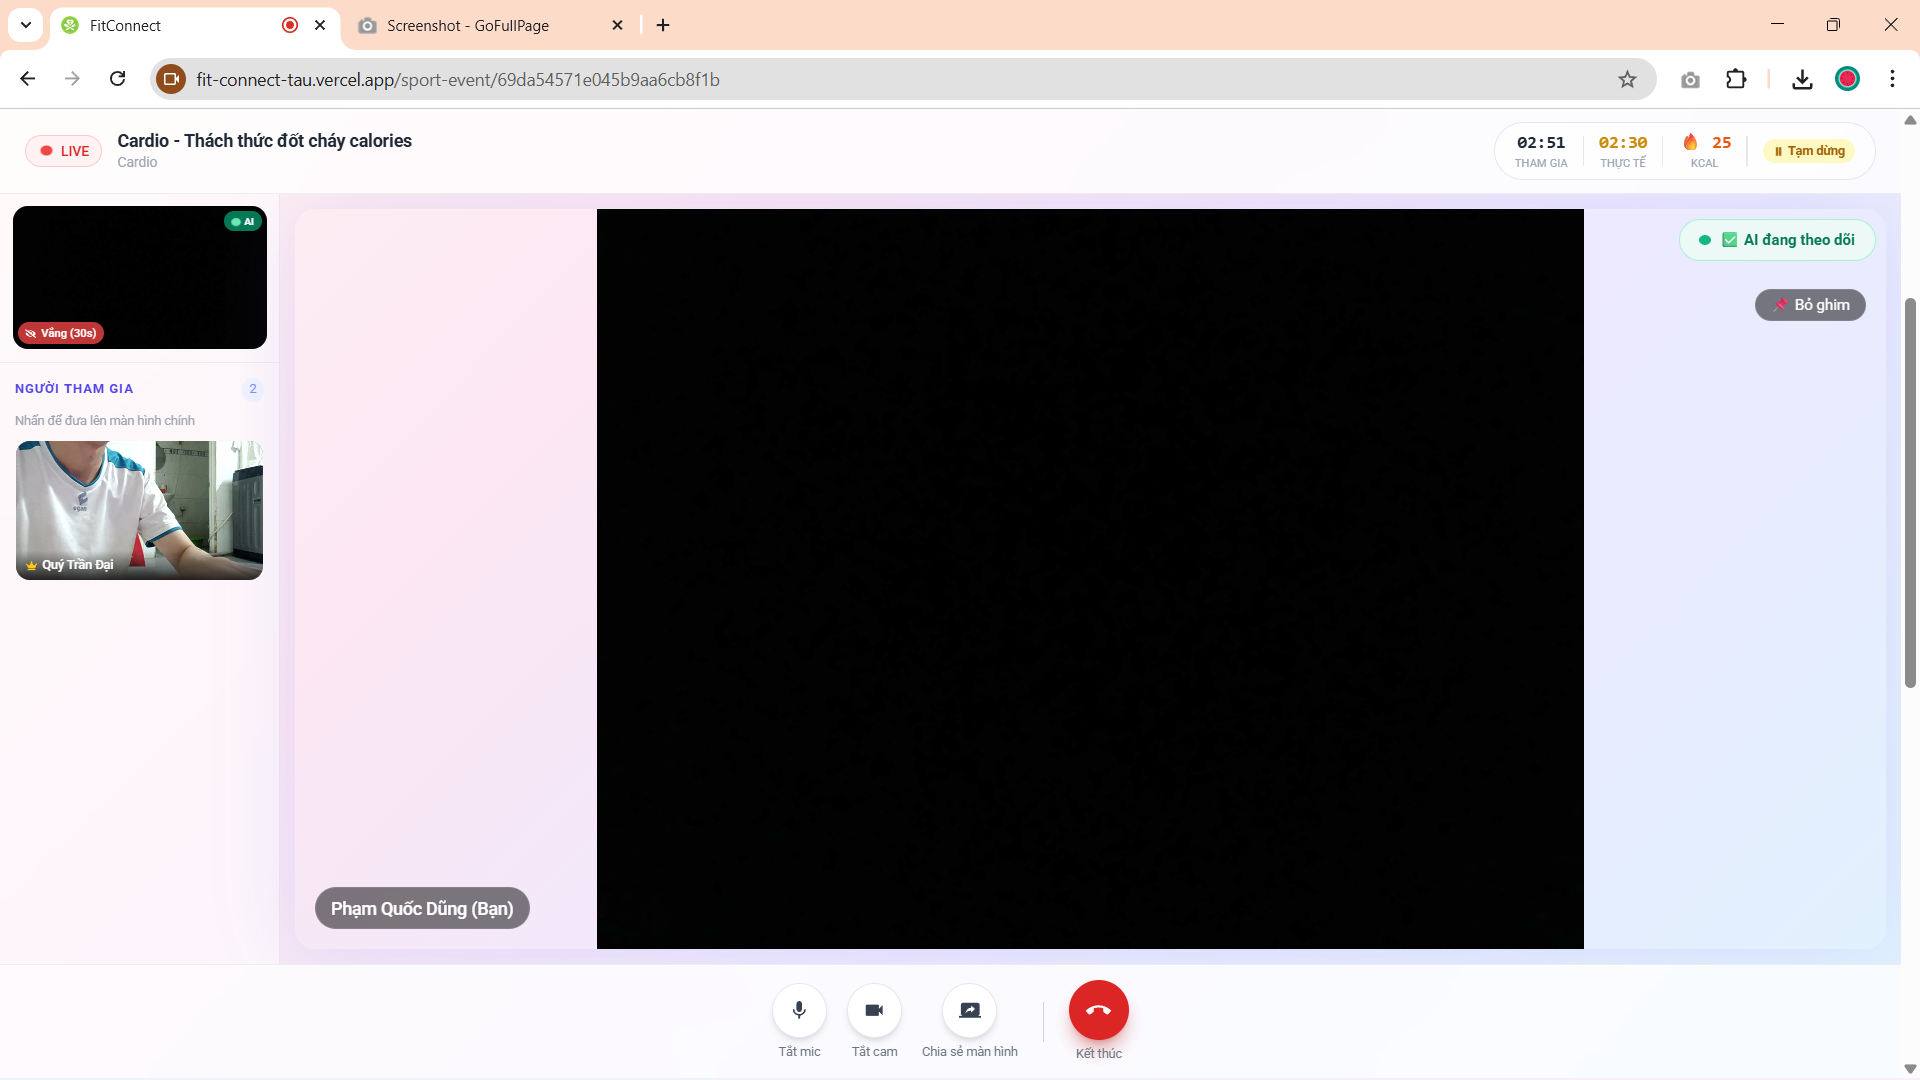
\includegraphics[width=0.60\textwidth]{Images/IMG/nhom3/checameraAInhandientamdung.png}
    \caption{Hệ thống AI nhận diện khuôn mặt và theo dõi sự hiện diện trong phiên Video Call}
    \label{fig:impl_ai_face}
\end{figure}

\subsubsection{Xác minh ảnh bữa ăn trong thử thách ăn uống}

Trong thử thách loại Ăn uống, khi người tham gia check-in bữa ăn bằng ảnh, hệ thống sử dụng AI đa phương thức (thị giác kết hợp ngôn ngữ) để xác minh ảnh có phải bữa ăn hợp lệ theo ngữ cảnh thử thách hay không, trả về ``Ảnh hợp lệ'' (tính tiến độ) hoặc ``Ảnh không phù hợp'' (không tính). Chi tiết tại mục~\ref{subsec:impl_challenge}.

\subsection{Tạo nội dung tự động bằng AI}
\label{subsec:impl_ai_auto_content}

Hệ thống tích hợp AI sinh nội dung (Google Gemini) để giảm thiểu thao tác nhập liệu thủ công trong hai tình huống:

\begin{itemize}
    \item \textbf{Sự kiện thể thao:} Người dùng mô tả ý tưởng bằng ngôn ngữ tự nhiên, AI tự động điền tên, loại sự kiện, địa điểm, thời gian, mô tả chi tiết và ảnh minh họa. Chi tiết tại mục~\ref{subsec:impl_sport_event}.
    \item \textbf{Thử thách cộng đồng:} Chọn loại thử thách (Ngoài trời / Ăn uống / Thể dục) và mô tả ý tưởng; AI điền tên, danh mục, mục tiêu mỗi ngày, thời gian và mô tả. Chi tiết tại mục~\ref{subsec:impl_challenge}.
\end{itemize}

\subsection{Phân tích sức khỏe và gợi ý bài tập cá nhân hóa}
\label{subsec:impl_ai_health_suggest}

Tại trang Công cụ tính toán sức khỏe, sau khi người dùng tính các chỉ số (BMI, TDEE, Body Fat,...), nút ``AI Phân Tích Sức Khỏe'' gửi các chỉ số lên AI để nhận đánh giá tổng quan, lời khuyên dinh dưỡng và danh sách bài tập phù hợp từ kho bài tập hệ thống.

\begin{figure}[H]
    \centering
    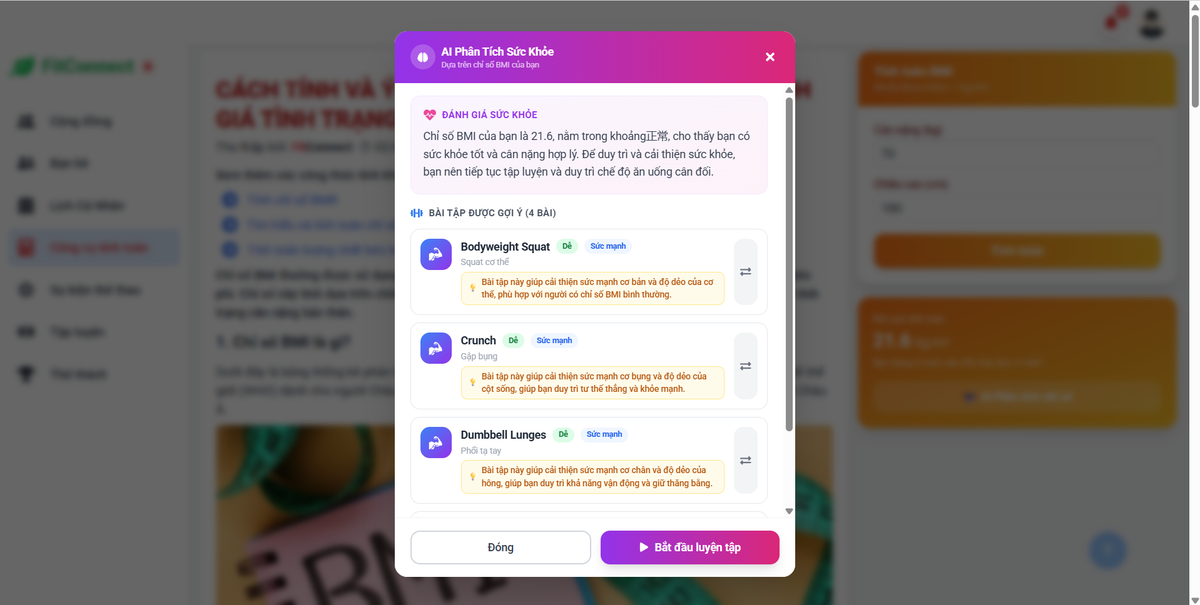
\includegraphics[width=0.60\textwidth]{Images/IMG/Congcusuckhoe/AIphantichsuckhoe.png}
    \caption{Hệ thống AI phân tích sức khỏe và gợi ý bài tập dựa trên chỉ số BMI}
    \label{fig:impl_ai_health}
\end{figure}

Tại trang Tập luyện, tính năng ``AI Gợi ý Tập Luyện'' cho phép người dùng mô tả tình trạng sức khỏe bằng ngôn ngữ tự nhiên (ví dụ: ``Tôi bị đau lưng, gợi ý bài tập phù hợp''). AI kết hợp mô tả với kho bài tập trong CSDL để trả về lời khuyên chi tiết và danh sách bài tập kèm lý do phù hợp. Người dùng chọn bài tập, sắp xếp thứ tự và nhấn ``Bắt đầu luyện tập''.

\begin{figure}[H]
    \centering
    \begin{subfigure}[b]{0.30\textwidth}
        \centering
        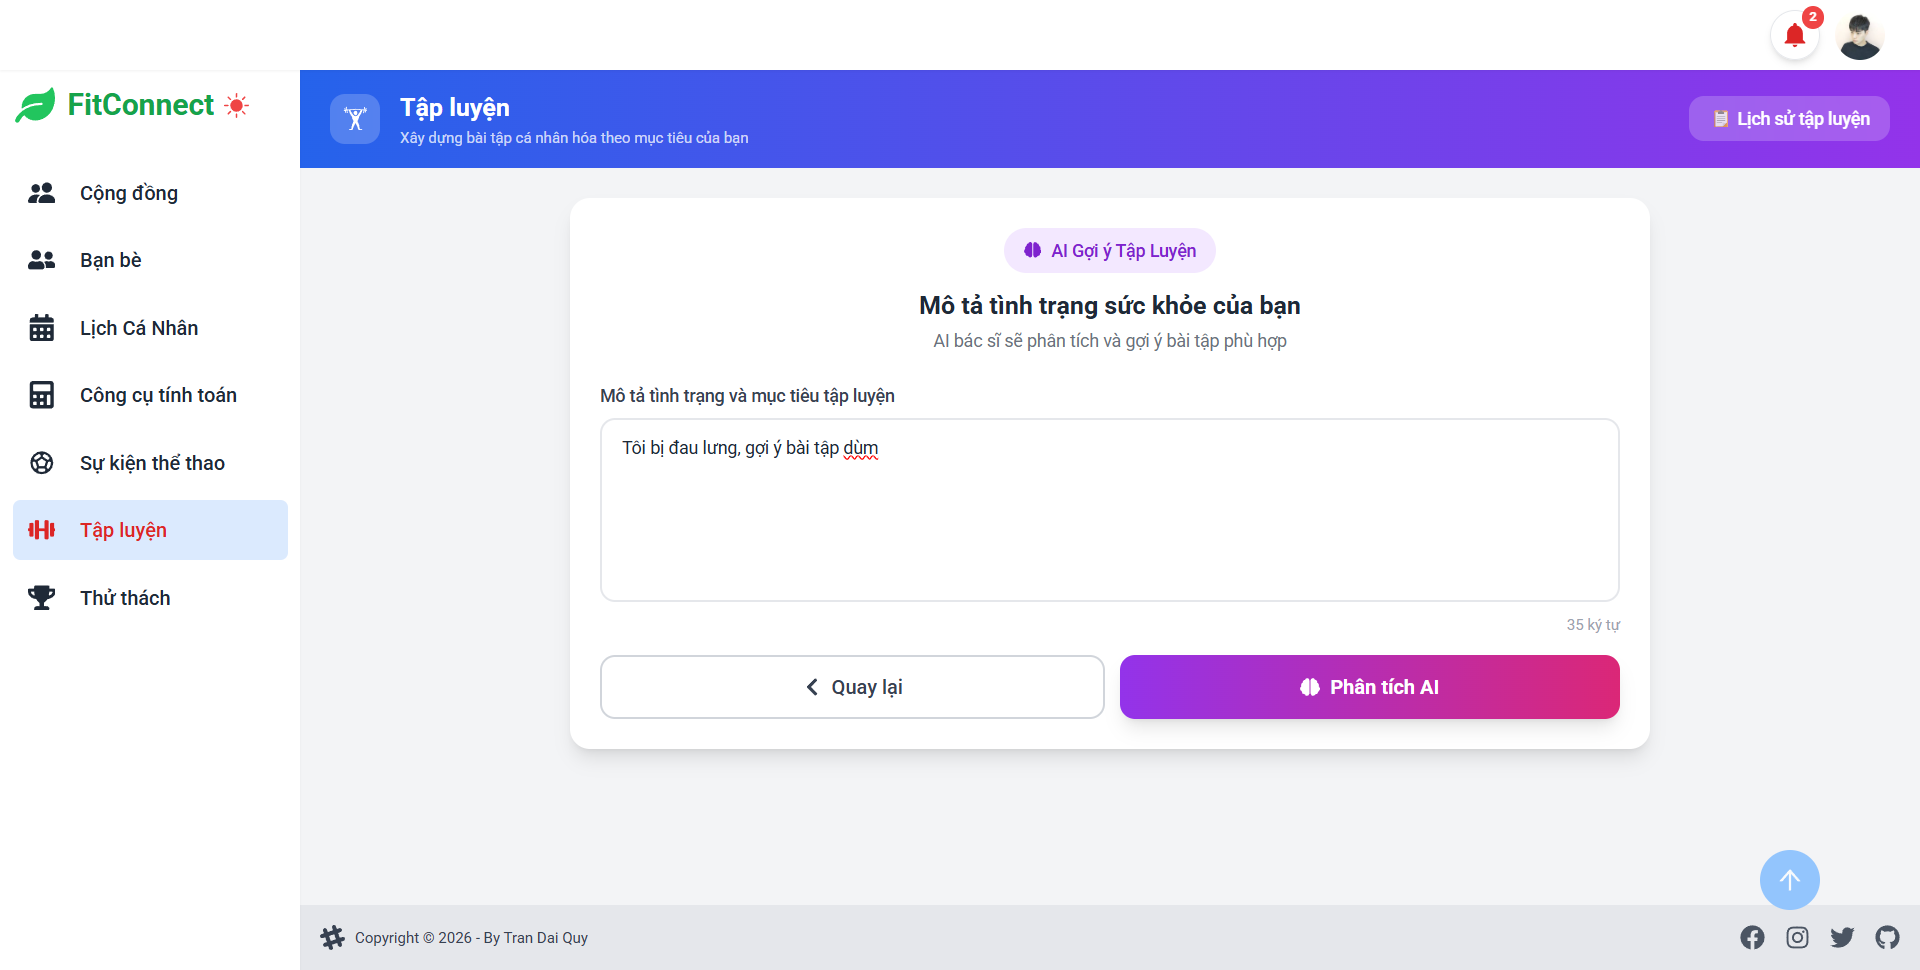
\includegraphics[width=\textwidth]{Images/IMG/Tapluyen/AIgoiytapluyen.png}
        \caption{Người dùng mô tả tình trạng sức khỏe để AI gợi ý bài tập}
        \label{fig:impl_ai_suggest_input}
    \end{subfigure}
    \hfill
    \begin{subfigure}[b]{0.30\textwidth}
        \centering
        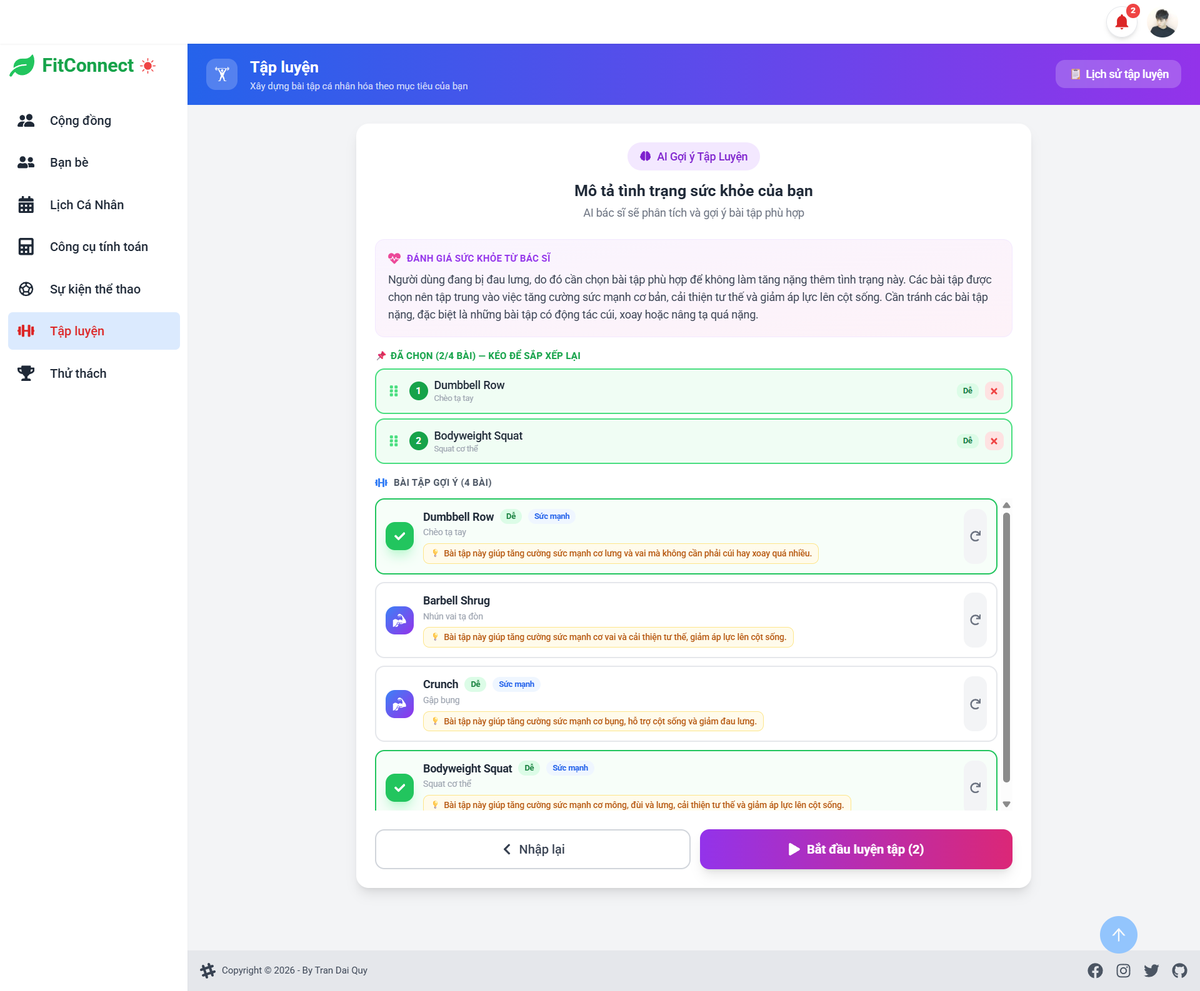
\includegraphics[width=\textwidth]{Images/IMG/Tapluyen/AIgoiytapluyen2.png}
        \caption{Hệ thống AI trả về đánh giá sức khỏe và danh sách bài tập gợi ý}
        \label{fig:impl_ai_suggest_result}
    \end{subfigure}
    \hfill
    \begin{subfigure}[b]{0.30\textwidth}
        \centering
        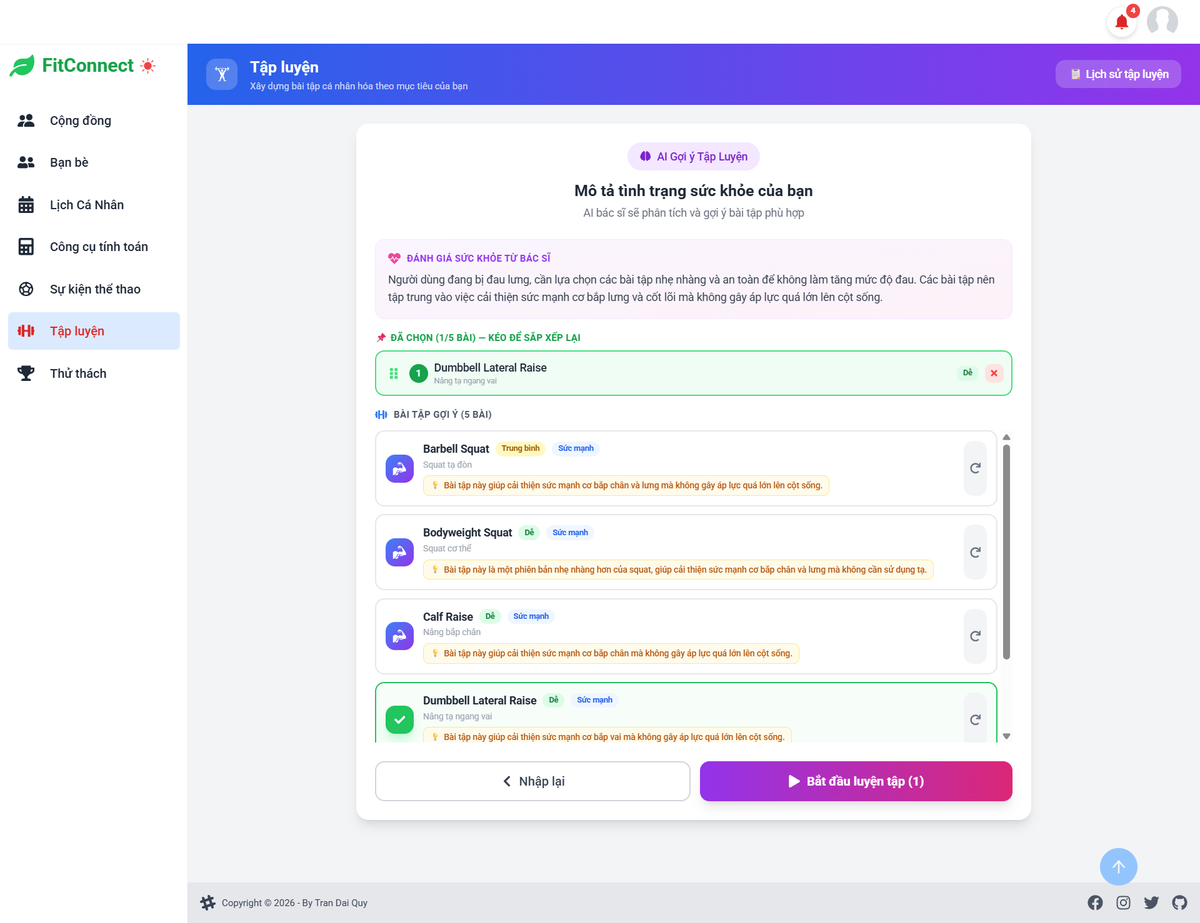
\includegraphics[width=\textwidth]{Images/IMG/nhom5/aigoigoiydanhsachbaitap.png}
        \caption{Người dùng chọn bài tập từ danh sách gợi ý AI và bắt đầu luyện tập}
        \label{fig:impl_ai_suggest_select}
    \end{subfigure}
\end{figure}

\subsection{Ghi nhận và thống kê sử dụng AI}
\label{subsec:impl_ai_usage}

Mọi lần gọi AI thành công đều được hệ thống ghi nhận vào cơ sở dữ liệu (phân loại theo tính năng: tạo sự kiện, tạo thử thách, gợi ý bài tập, xác minh ảnh bữa ăn,...). Dữ liệu này được tổng hợp và hiển thị trên bảng điều khiển Quản trị viên, giúp theo dõi tần suất sử dụng AI theo từng tính năng, đánh giá hiệu quả và tối ưu hóa hệ thống.

\section{Hiện thực các nhóm tính năng}
\label{sec:impl_features}

Hệ thống FitConnect được xây dựng như một hệ sinh thái rèn luyện thể chất toàn diện, bao gồm 9 nhóm tính năng cốt lõi có mối quan hệ tương hỗ chặt chẽ với nhau. Sự kết nối này đảm bảo luồng dữ liệu thông suốt: từ việc định danh người dùng (Account), kết nối cộng đồng (Community, Friends), đến việc tổ chức các hoạt động thi đua (Sport Events, Challenges) và cá nhân hóa lộ trình tập luyện (Training, Health Metrics, AI Suggestions) dựa trên lịch trình thống nhất (Calendar).

Mối quan hệ giữa 9 nhóm tính năng này được thể hiện trực quan qua Hình \ref{fig:impl_feature_overview}, minh chứng cho triết lý thiết kế ``Dữ liệu làm nền tảng -- AI dẫn dắt -- Cộng đồng lan tỏa'' của nền tảng.


\begin{figure}[H]
    \centering
    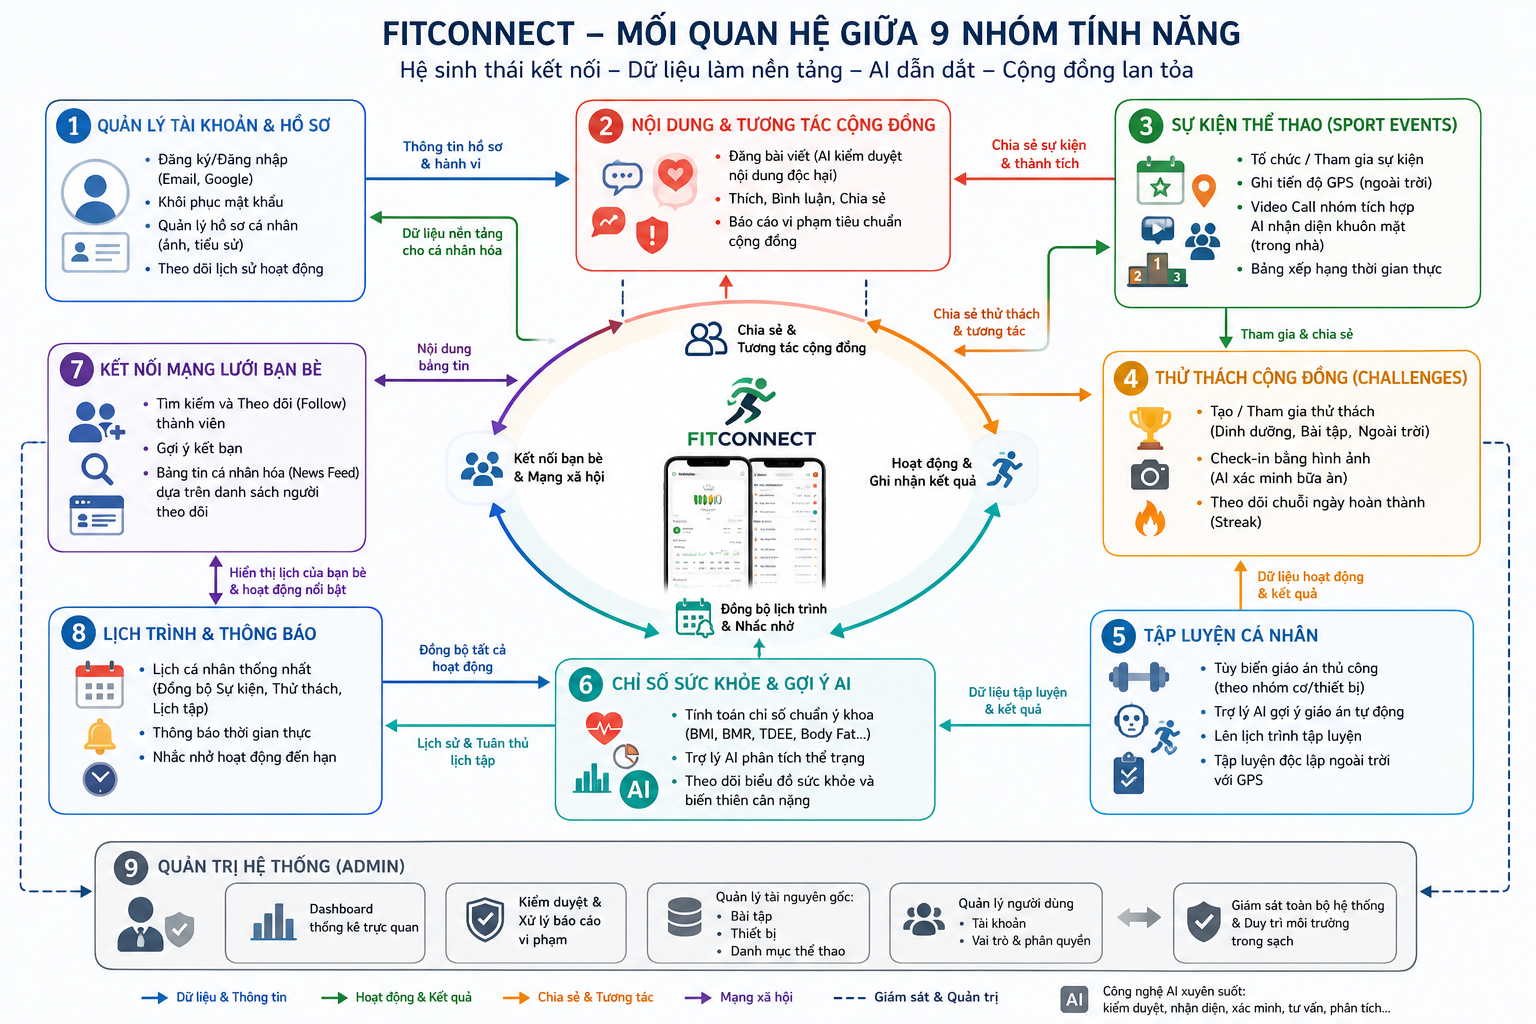
\includegraphics[width=0.60\textwidth]{Images/IMG/Motahethong.png}
    \caption{Sơ đồ tổng quan mối quan hệ tương hỗ giữa 9 nhóm tính năng trong hệ sinh thái FitConnect}
    \label{fig:impl_feature_overview}
\end{figure}


Dưới đây là phần hiện thực chi tiết kết quả của từng nhóm tính năng cốt lõi cấu thành hệ thống. Mỗi tính năng được phân tích theo \textbf{Luồng xử lý (Workflow)} kết hợp kiến trúc kỹ thuật và minh họa trực quan từ giao diện ứng dụng thực tế.

\subsection{Nhóm tính năng Quản lý Tài khoản \& Hồ sơ (Account \& Profile)}
\label{subsec:impl_account}

Đây là nhóm chức năng đóng vai trò định danh, cá nhân hóa không gian hoạt động của người dùng, và bảo mật quyền truy cập toàn rải hệ thống. Quá trình hoạt động được chia thành 3 luồng chính.

\subsubsection{Luồng Đăng ký và Đăng nhập hệ thống}
\textbf{Mục tiêu:} Kiểm soát quyền truy cập qua cơ chế JWT, ngăn chặn tấn công giả mạo và cung cấp khả năng Login nhanh thông qua hệ sinh thái Google.
\textbf{Luồng xử lý kỹ thuật:}
\begin{enumerate}
    \item \textbf{Đăng ký tài khoản (Hình \ref{fig:impl_register}):} Người dùng cung cấp thư điện tử (Email), mật khẩu và các thông tin cơ bản. Ứng dụng tiến hành kiểm tra tính hợp lệ của dữ liệu đầu vào theo thời gian thực trước khi gửi yêu cầu đến máy chủ. Tại phía máy chủ, thông tin xác thực được xử lý bằng thuật toán băm (Hash) kết hợp kỹ thuật thêm chuỗi ngẫu nhiên (Salt) nhằm đảm bảo an toàn tuyệt đối trước khi lưu trữ vào cơ sở dữ liệu.
    \item \textbf{Đăng nhập và định danh (Hình \ref{fig:impl_login}):} Quá trình đăng nhập hỗ trợ hai phương thức: xác thực truyền thống qua thư điện tử và xác thực bên thứ ba thông qua hệ sinh thái Google (OAuth 2.0). Khi định danh thành công, hệ thống cấp phát một chứng thư số điện tử dạng mã thông báo (Access Token) có thời hạn sử dụng xác định. Chứng thư này được ứng dụng phía máy khách lưu giữ và đính kèm tự động vào thao tác giao tiếp tiếp theo để duy trì trạng thái phiên hoạt động.
\end{enumerate}


\begin{figure}[H]
    \centering
    \begin{subfigure}[b]{0.30\textwidth}
        \centering
        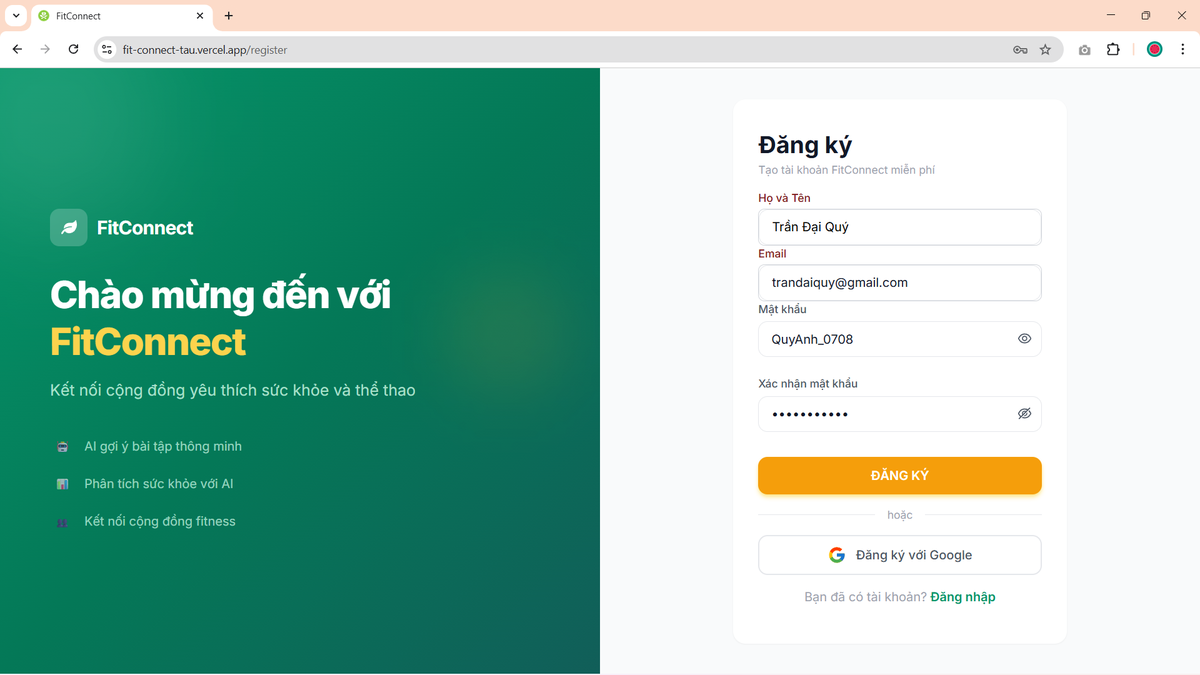
\includegraphics[width=\textwidth]{Images/IMG/Nhom1/dangky.png}
        \caption{Giao diện Đăng ký thành viên FitConnect}
        \label{fig:impl_register}
    \end{subfigure}
    \hfill
    \begin{subfigure}[b]{0.30\textwidth}
        \centering
        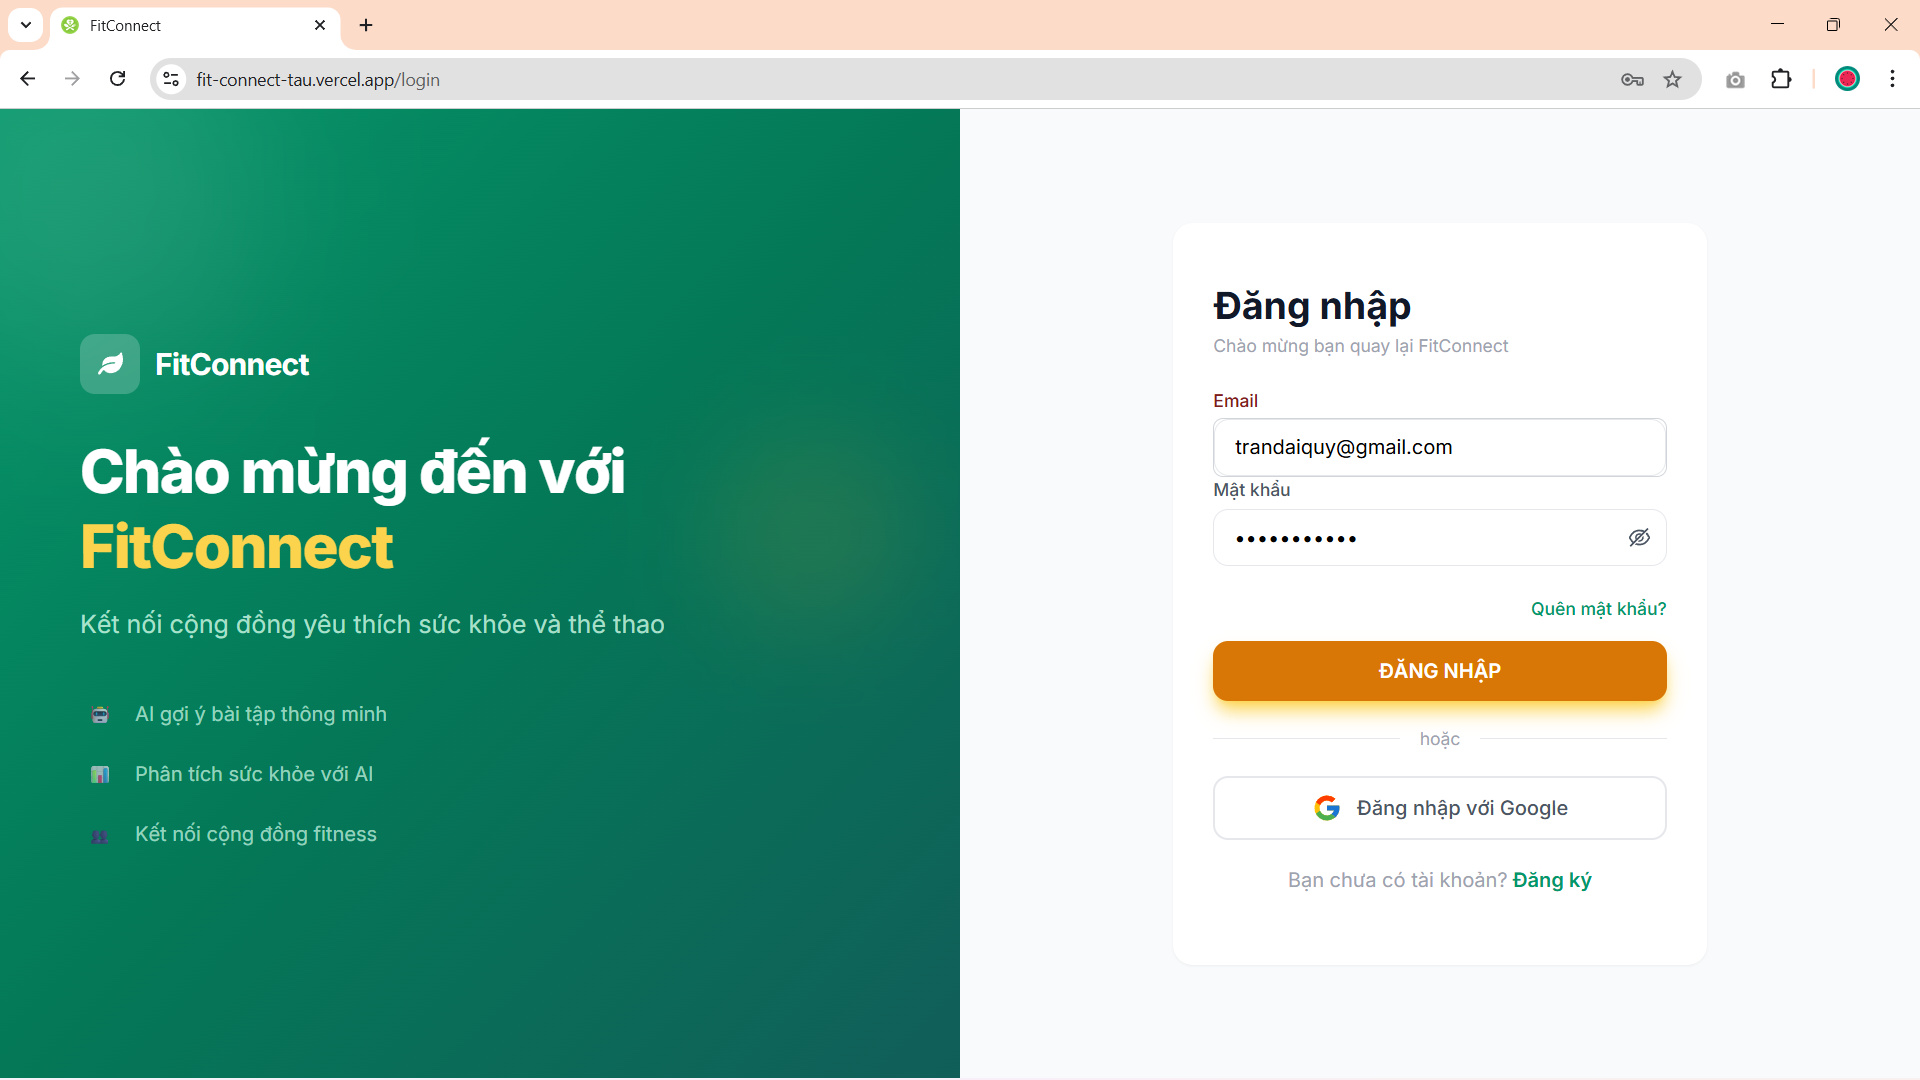
\includegraphics[width=\textwidth]{Images/IMG/Nhom1/dangnhap.png}
        \caption{Giao diện Đăng nhập hệ thống}
        \label{fig:impl_login}
    \end{subfigure}
    \hfill
    \begin{subfigure}[b]{0.30\textwidth}
        \centering
        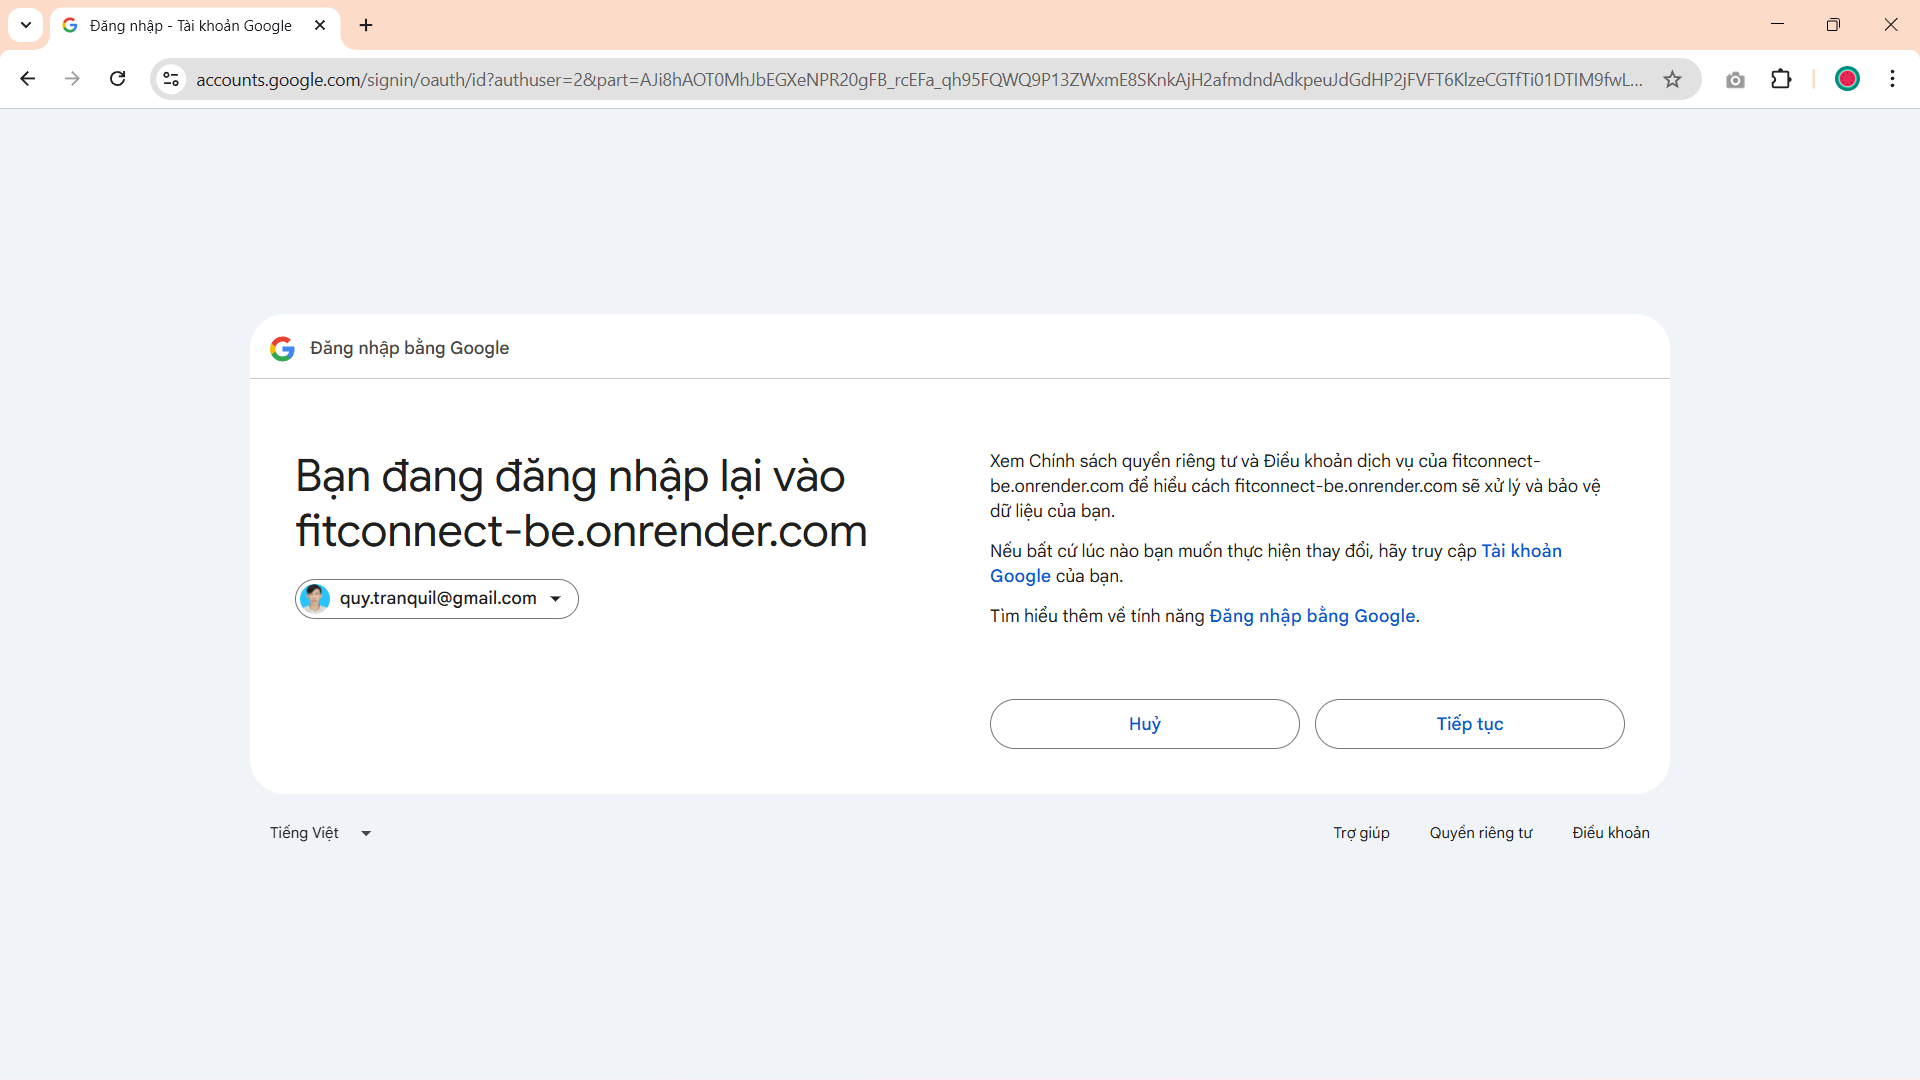
\includegraphics[width=\textwidth]{Images/IMG/Nhom1/logingoogle.png}
        \caption{Lựa chọn Xác thực tài khoản nhanh qua Google OAuth}
        \label{fig:impl_login_google}
    \end{subfigure}
\end{figure}

Sau khi xác thực thành công, hệ thống cấp phát Access Token và tự động điều hướng người dùng về Trang chủ (Home) với bảng tin cộng đồng.


\subsubsection{Luồng Xác thực OTP và Khôi phục mật khẩu}
\textbf{Mục tiêu:} Hỗ trợ người dùng khôi phục quyền truy cập tài khoản một cách an toàn thông qua quy trình xác minh hai bước bằng mã sử dụng một lần (OTP - One-Time Password) gửi qua thư điện tử.
\textbf{Quy trình hoạt động:}
\begin{enumerate}
    \item \textbf{Yêu cầu thiết lập lại (Hình \ref{fig:impl_forgot_pw}):} Hệ thống tiếp nhận thư điện tử do người dùng cung cấp và đối chiếu với cơ sở dữ liệu. Nếu tài khoản khả dụng, một mã xác thực OTP ngẫu nhiên gồm 6 chữ số sẽ được khởi tạo với vòng đời được quản lý nghiêm ngặt trong 5 phút.
    \item \textbf{Điều phối thư điện tử (Hình \ref{fig:impl_send_otp}):} Thông qua dịch vụ gửi đám mây chuyên dụng, hệ thống tự động biên dịch và gửi thông điệp chứa mã bảo mật đến địa chỉ người dùng cung cấp.
    \item \textbf{Xác thực mã (Hình \ref{fig:impl_input_otp}):} Người dùng điền chuỗi mã gửi về vào giao diện ứng dụng. Hệ thống đối chiếu dữ liệu một cách trực tiếp với mã tại máy chủ; nếu hợp lệ, phiên làm việc sẽ được phê duyệt giới hạn để chuyển sang chặng thay đổi khóa.
    \item \textbf{Tạo mới mật khẩu (Hình \ref{fig:impl_forgot_pw_change}):} Ở thao tác cuối, người dùng tự ấn định một mật khẩu mới. Chuỗi thông tin này bắt buộc chạy qua quy trình băm độc lập trước khi đẩy lùi mật khẩu cũ để tái thiết lập rào chắn bảo vệ của hồ sơ.
\end{enumerate}


\begin{figure}[H]
    \centering
    \begin{subfigure}[b]{0.30\textwidth}
        \centering
        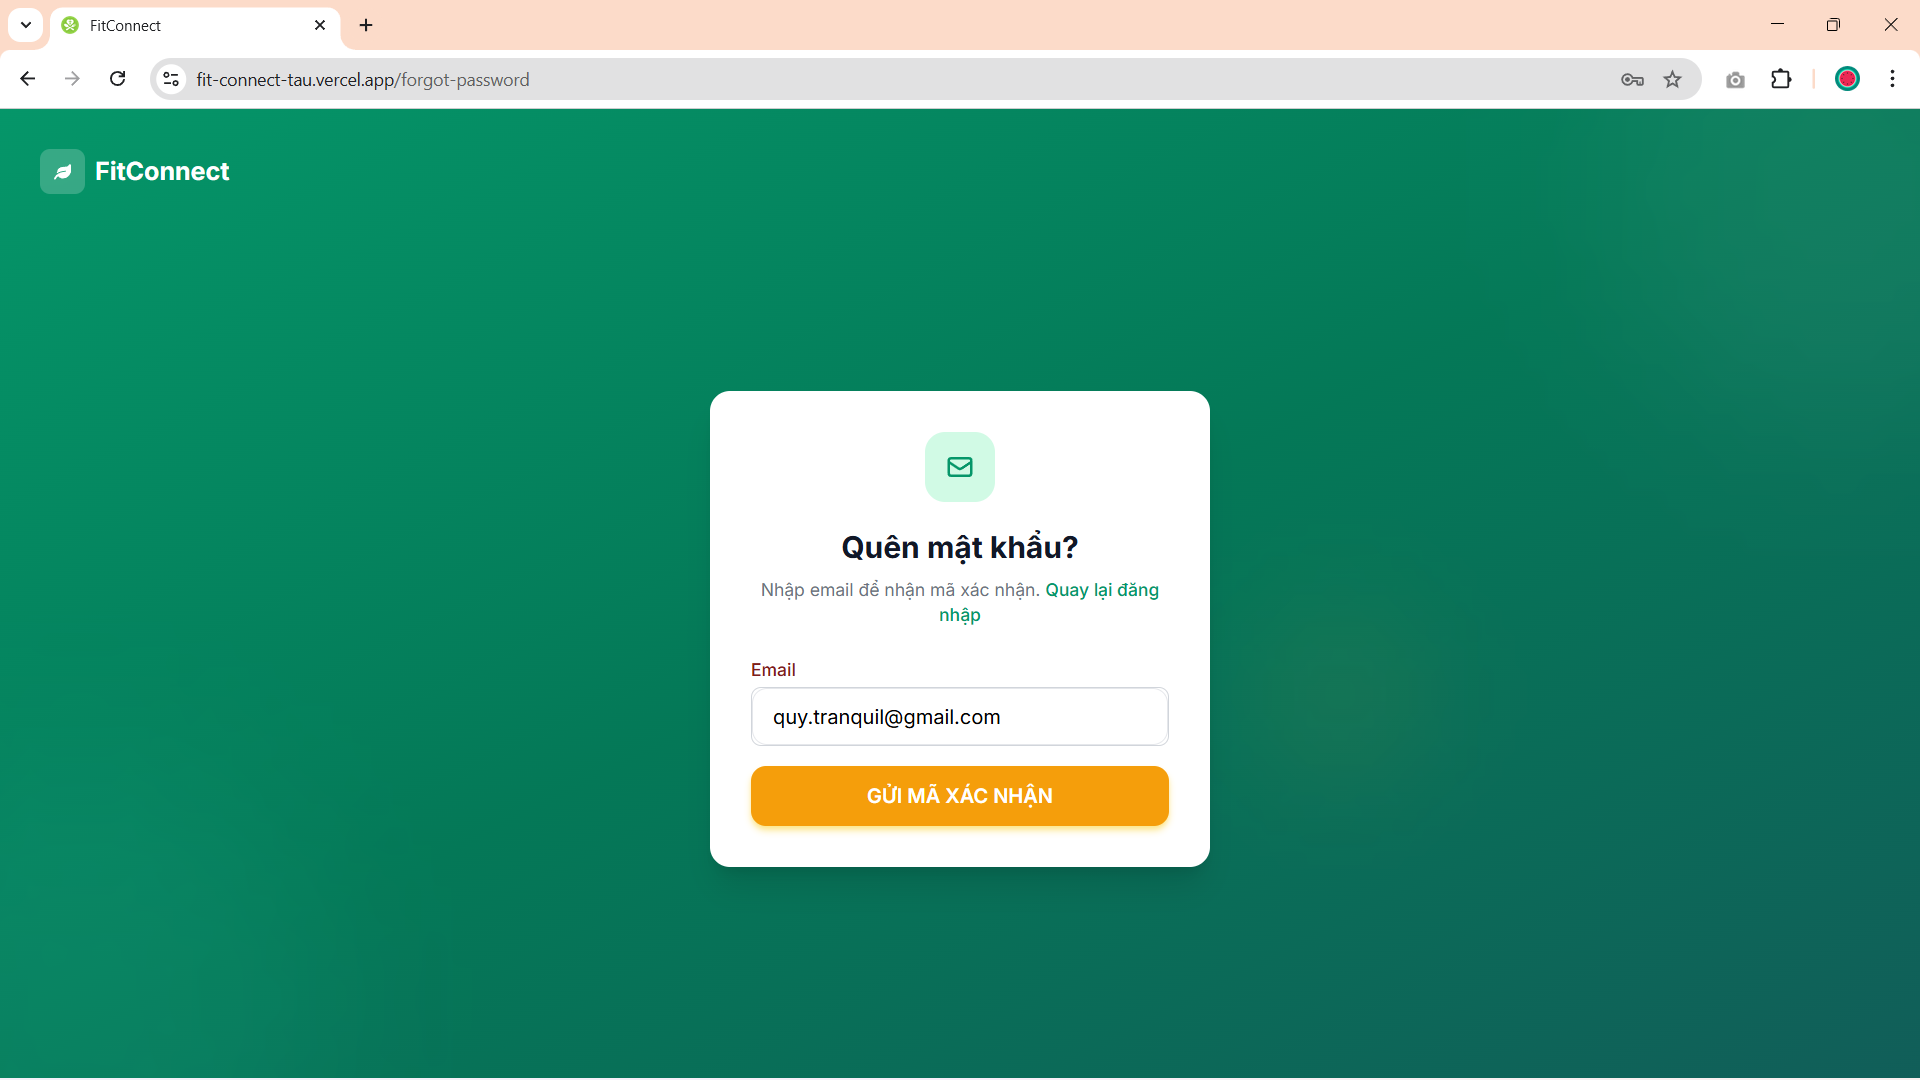
\includegraphics[width=\textwidth]{Images/IMG/Nhom1/quenmatkhau.png}
        \caption{Giao diện điền thông tin Yêu cầu khôi phục mật khẩu}
        \label{fig:impl_forgot_pw}
    \end{subfigure}
    \hfill
    \begin{subfigure}[b]{0.30\textwidth}
        \centering
        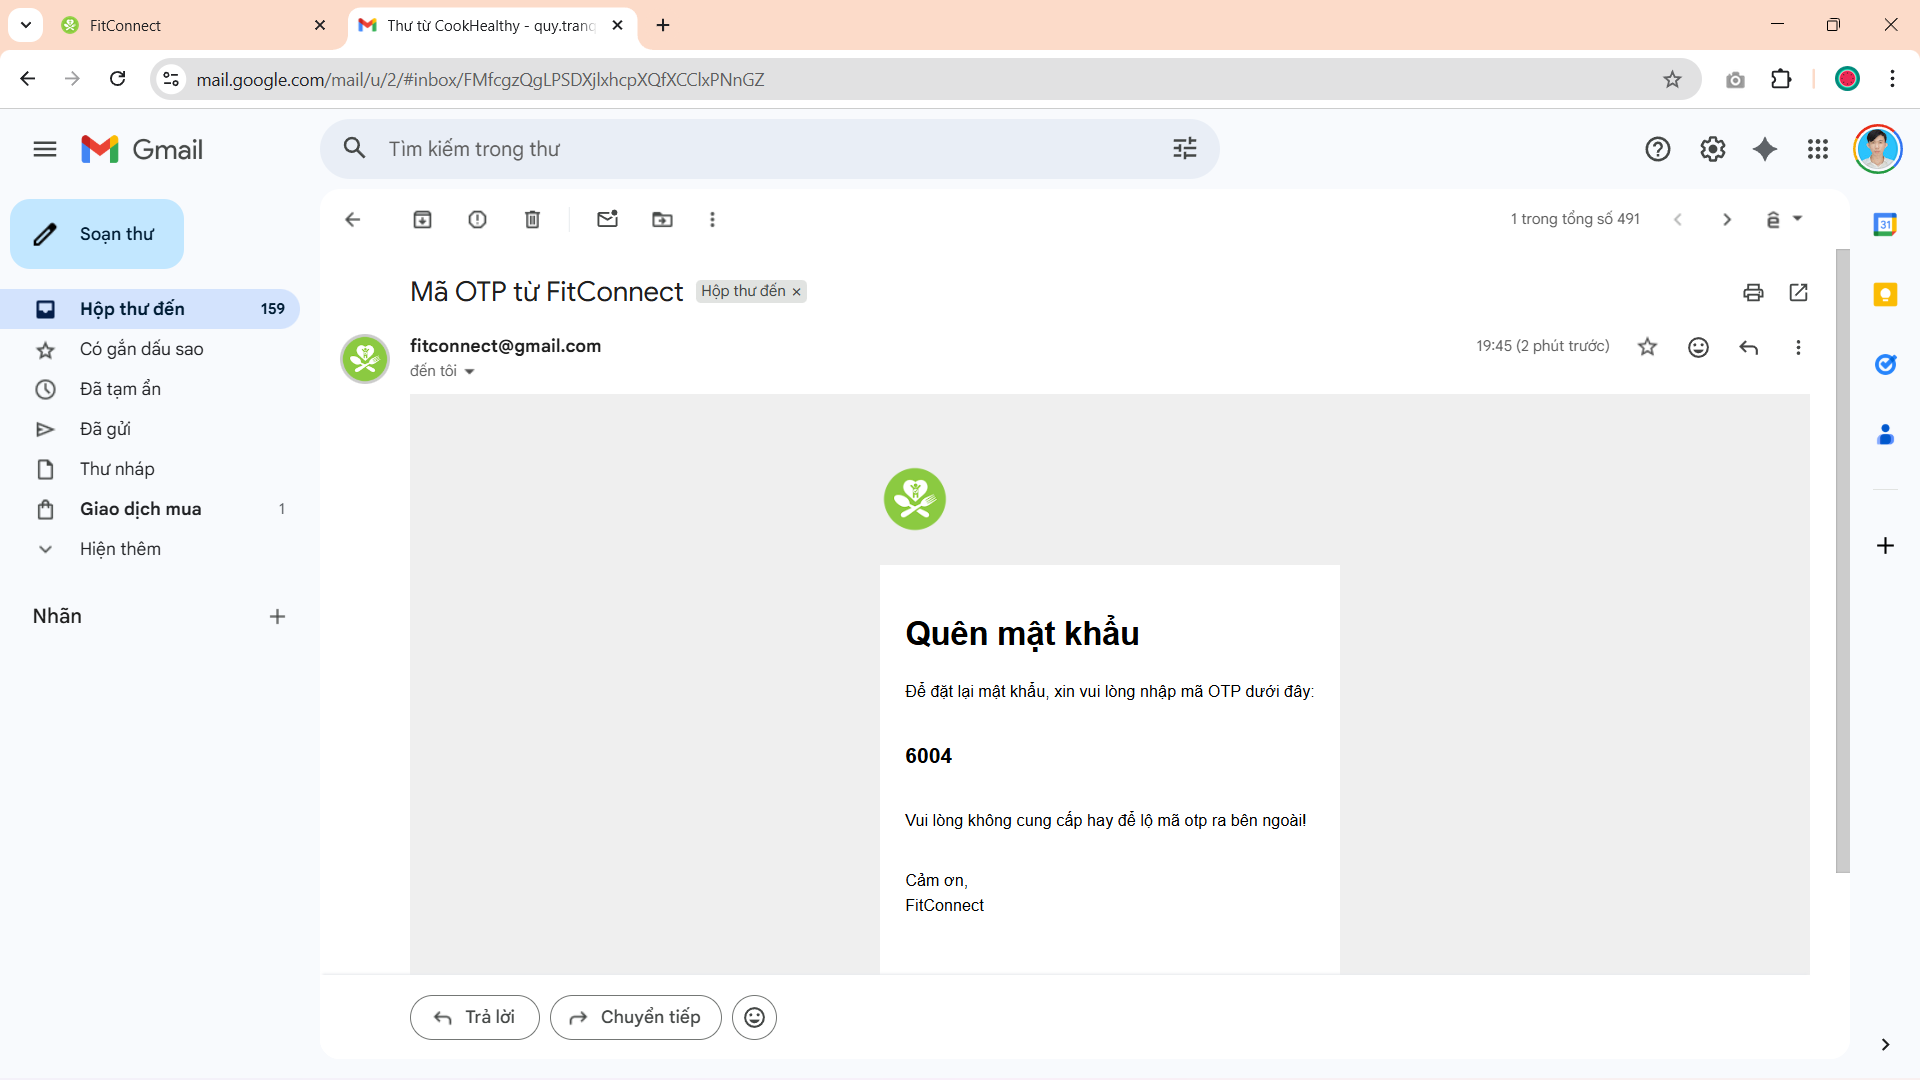
\includegraphics[width=\textwidth]{Images/IMG/Nhom1/guiotpveemail.png}
        \caption{Email tự động gửi dải mã OTP bảo mật 6 ký tự}
        \label{fig:impl_send_otp}
    \end{subfigure}
    \hfill
    \begin{subfigure}[b]{0.30\textwidth}
        \centering
        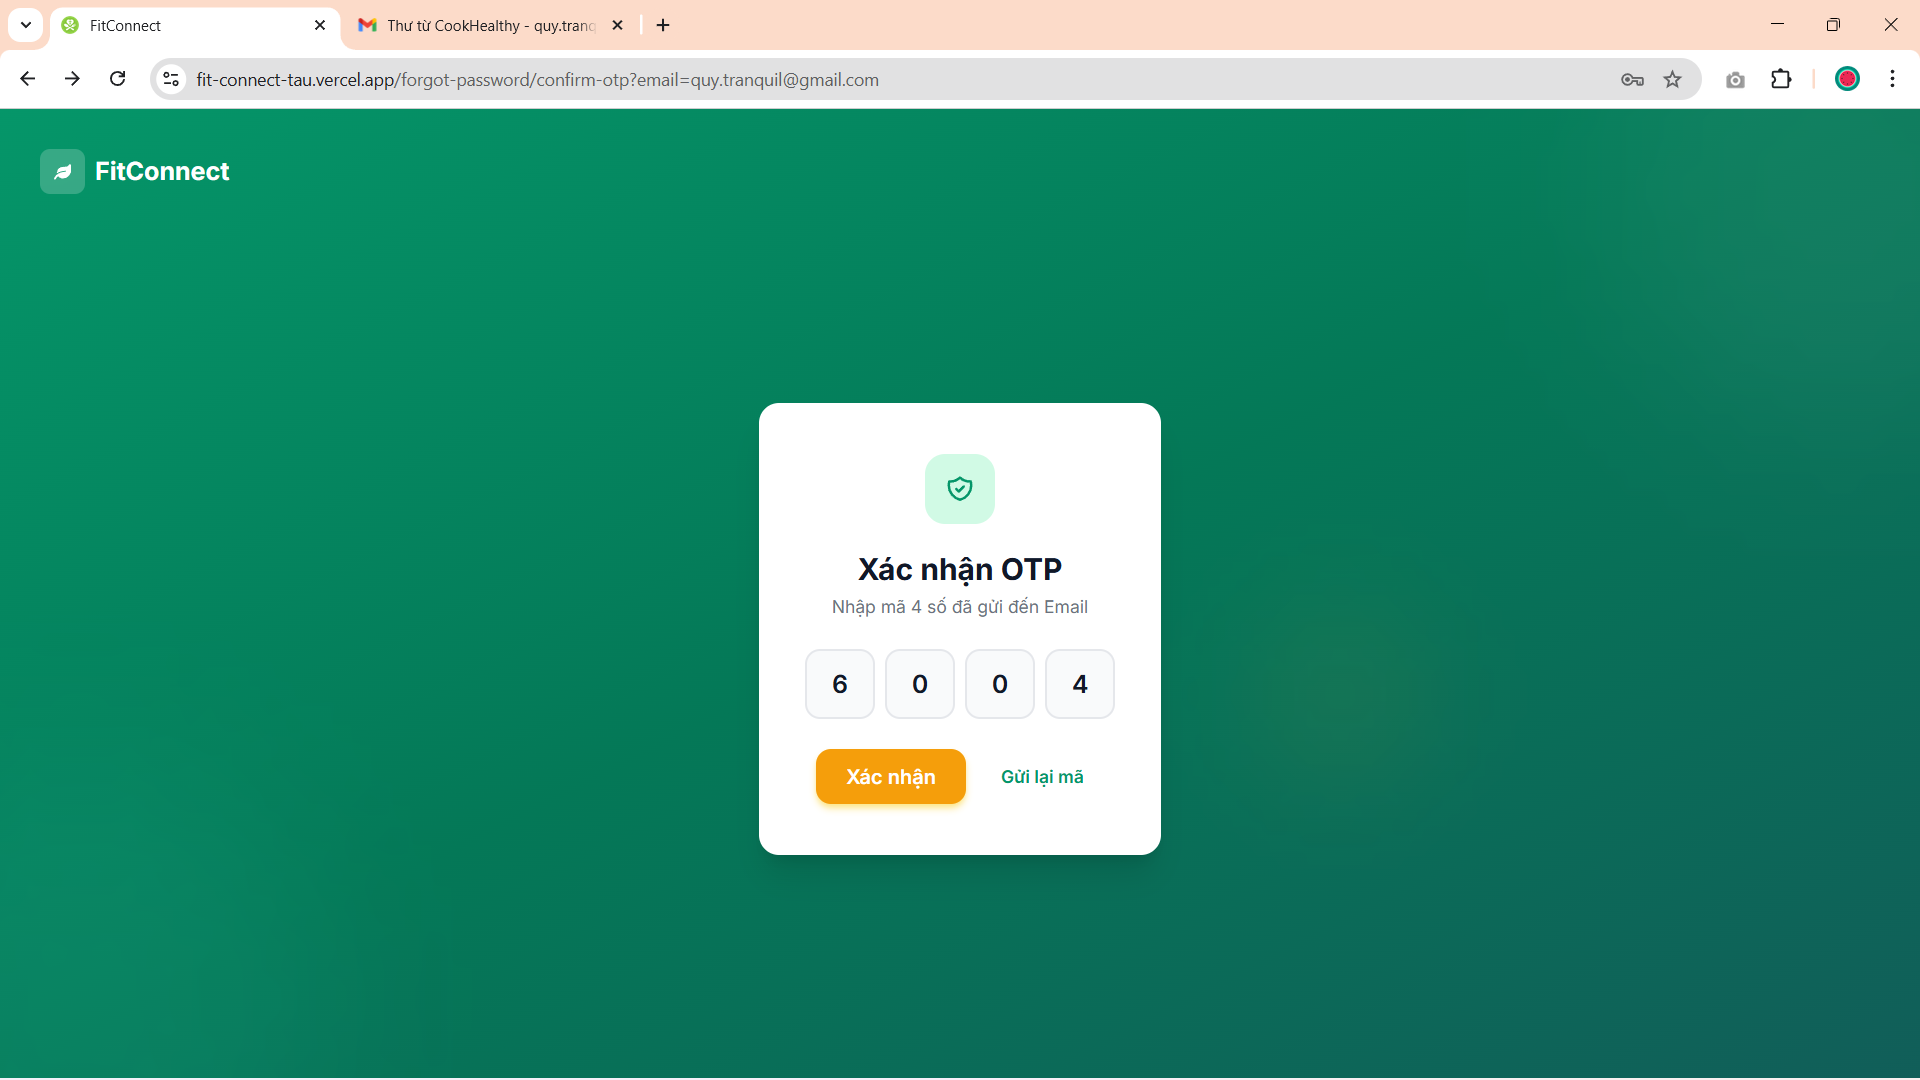
\includegraphics[width=\textwidth]{Images/IMG/Nhom1/nhapotp.png}
        \caption{Giao diện Frontend yêu cầu nhập mã OTP hợp lệ}
        \label{fig:impl_input_otp}
    \end{subfigure}
\end{figure}

\begin{figure}[H]
    \centering
    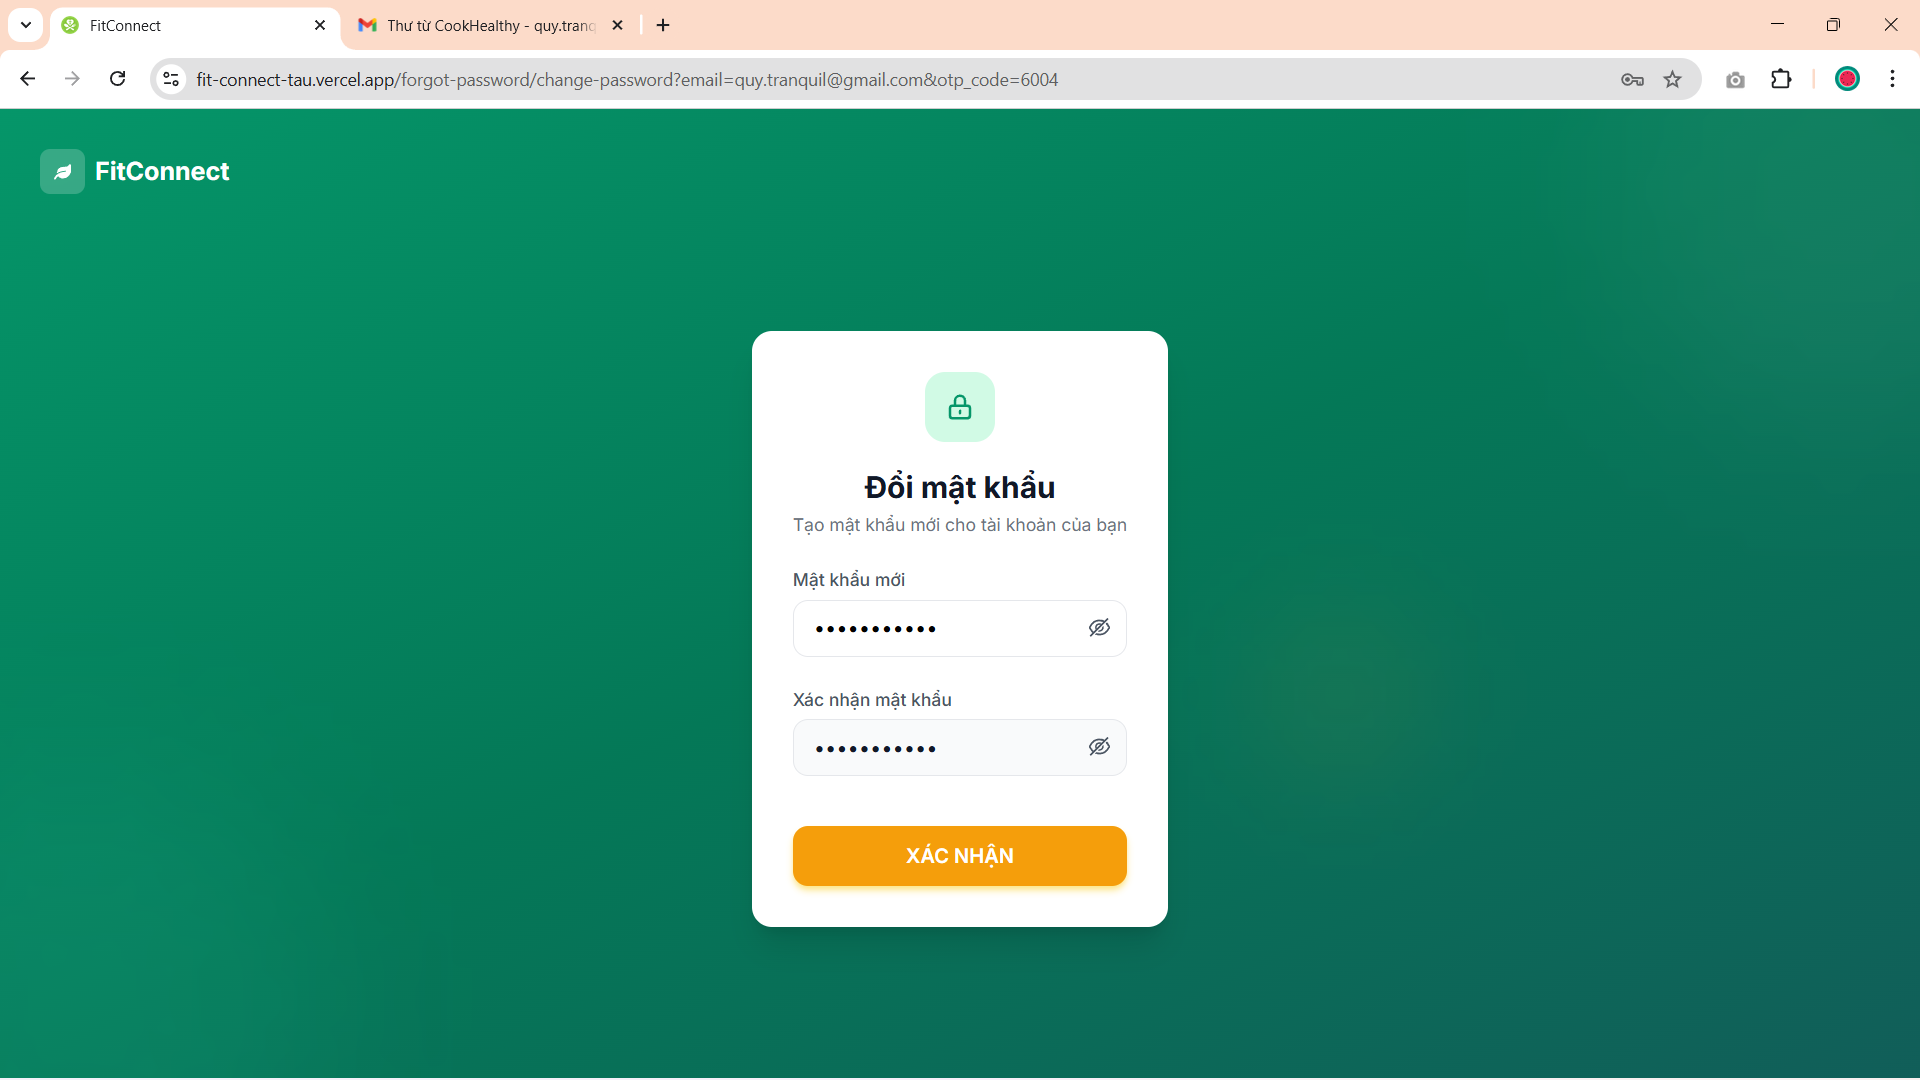
\includegraphics[width=0.60\textwidth]{Images/IMG/Nhom1/doimatkhau.png}
    \caption{Thiết lập mật khẩu mới và khôi phục quyền bảo vệ hoàn tất}
    \label{fig:impl_forgot_pw_change}
\end{figure}



\subsubsection{Luồng Quản trị Hồ sơ \& Tương tác cá nhân hóa (Profile Dashboard)}
\textbf{Mục tiêu:} Xây dựng không gian Profile Dashboard làm trung tâm quản trị hồ sơ cá nhân, nơi người dùng vừa theo dõi tổng quan hoạt động, vừa thực hiện các thao tác cá nhân hóa (ảnh đại diện, ảnh nền, thông tin hồ sơ, bảo mật tài khoản) ngay tại chỗ với số bước tối thiểu.

\textbf{Quy trình hoạt động:}
\begin{itemize}
    \item Người dùng truy cập trang cá nhân để xem thông tin hồ sơ tổng quát (ảnh đại diện, ảnh nền, mô tả, các chỉ số hoạt động). Đây là điểm vào chính của luồng quản trị hồ sơ và các thao tác cá nhân hóa.

\begin{figure}[H]
    \centering
    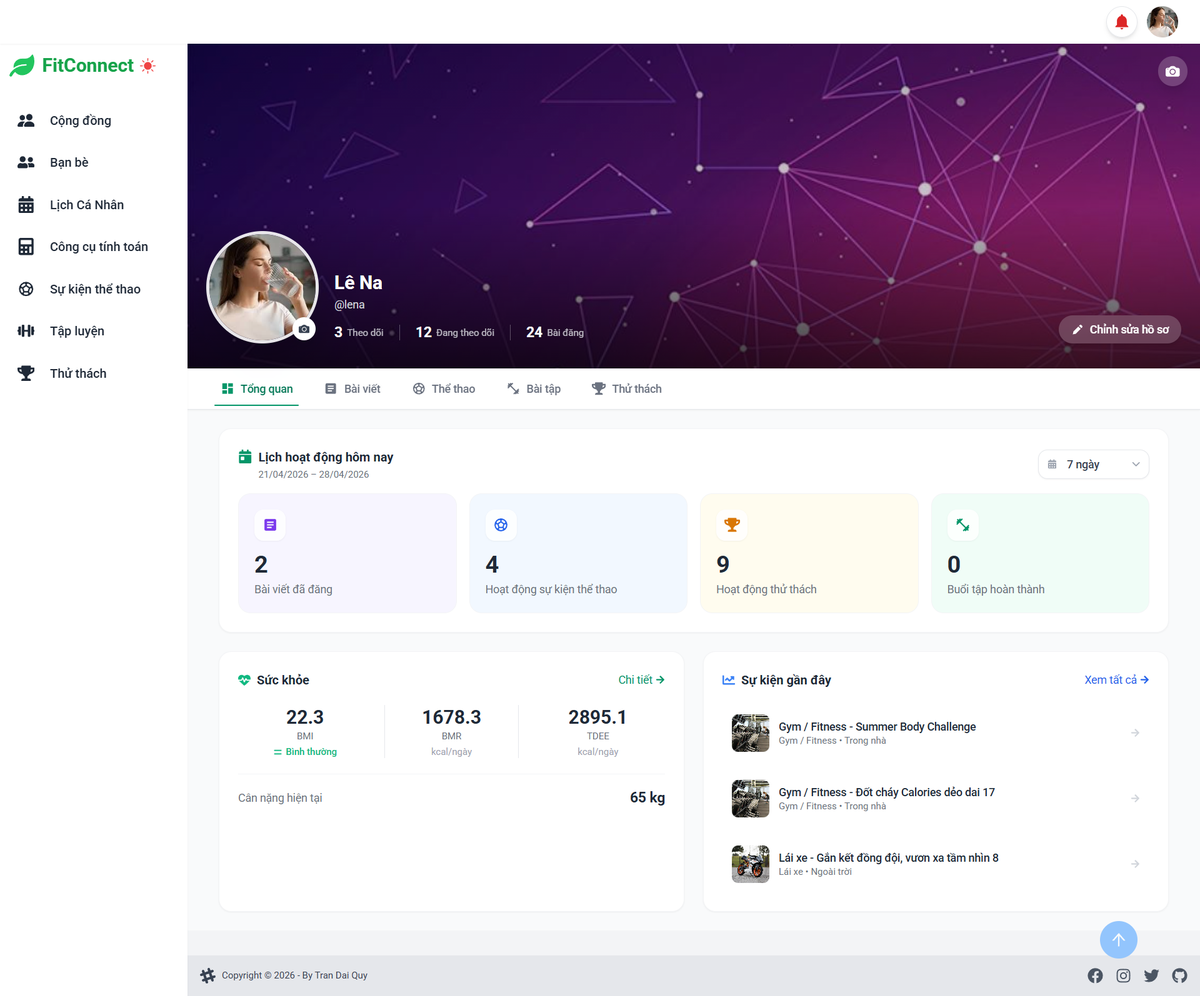
\includegraphics[width=0.60\textwidth]{Images/IMG/Nhom1/trangcanhan.png}
    \caption{Giao diện tổng quan trang cá nhân của người dùng}
    \label{fig:impl_profile_overview}
\end{figure}


    \item Trang cá nhân cung cấp ba tab chuyên biệt để theo dõi hoạt động: tab \textbf{Bài viết} hiển thị lịch sử bài đã đăng, tab \textbf{Sự kiện} tổng hợp sự kiện đã tham gia/tạo, và tab \textbf{Thử thách} tập trung mục tiêu và tiến độ hoàn thành.

\begin{figure}[H]
    \centering
    \begin{subfigure}[b]{0.30\textwidth}
        \centering
        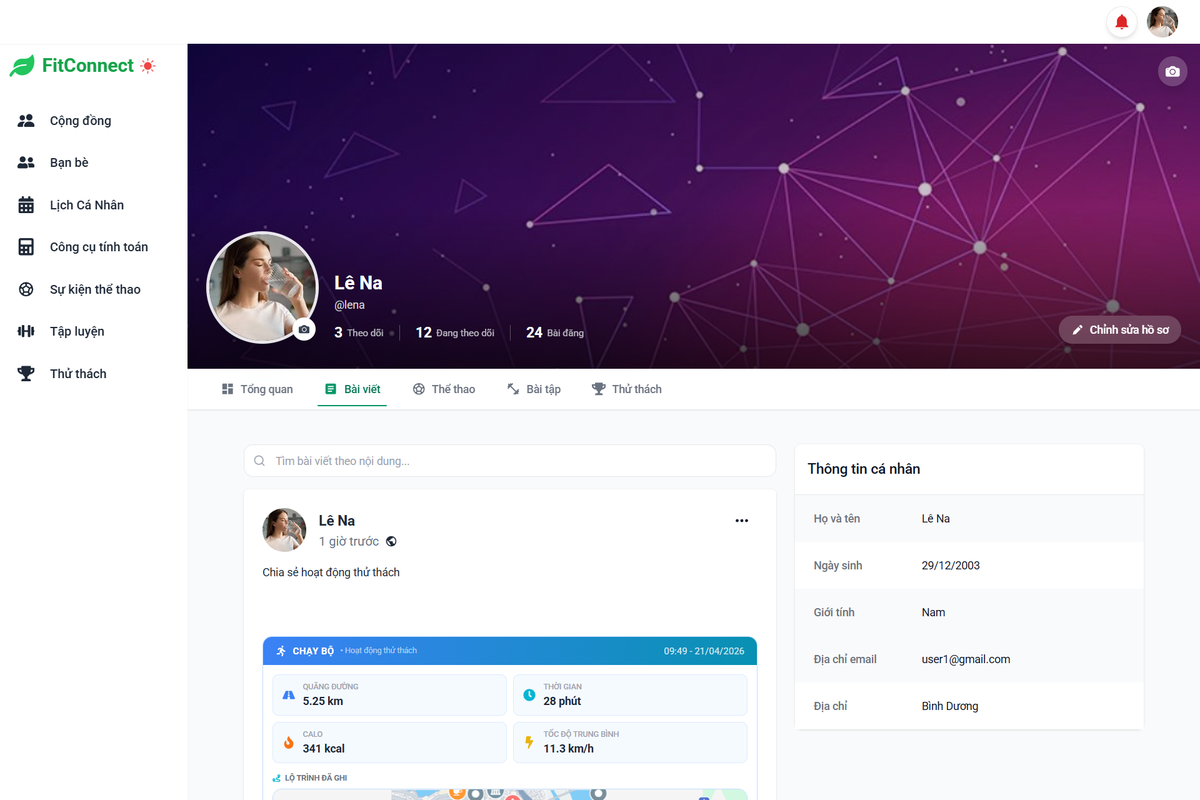
\includegraphics[width=\textwidth]{Images/IMG/Nhom1/tabtongquanbaiviet.png}
        \caption{Tab Bài viết}
        \label{fig:impl_profile_posts_tab}
    \end{subfigure}
    \hfill
    \begin{subfigure}[b]{0.30\textwidth}
        \centering
        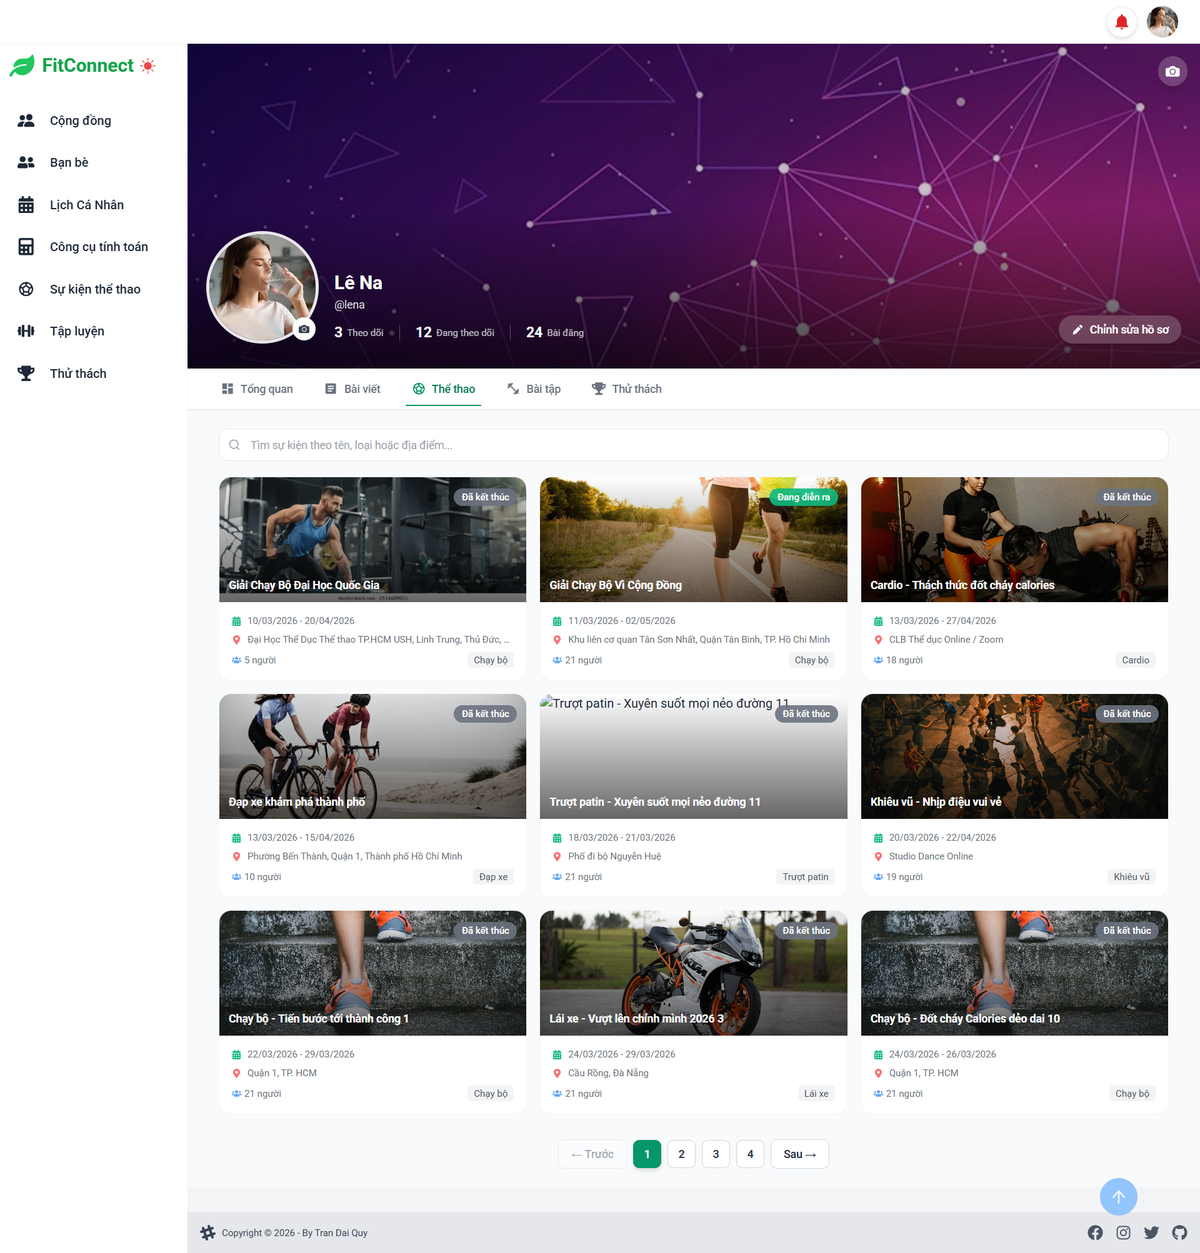
\includegraphics[width=\textwidth]{Images/IMG/Nhom1/tabsukien.png}
        \caption{Tab Sự kiện}
        \label{fig:impl_profile_events_tab}
    \end{subfigure}
    \hfill
    \begin{subfigure}[b]{0.30\textwidth}
        \centering
        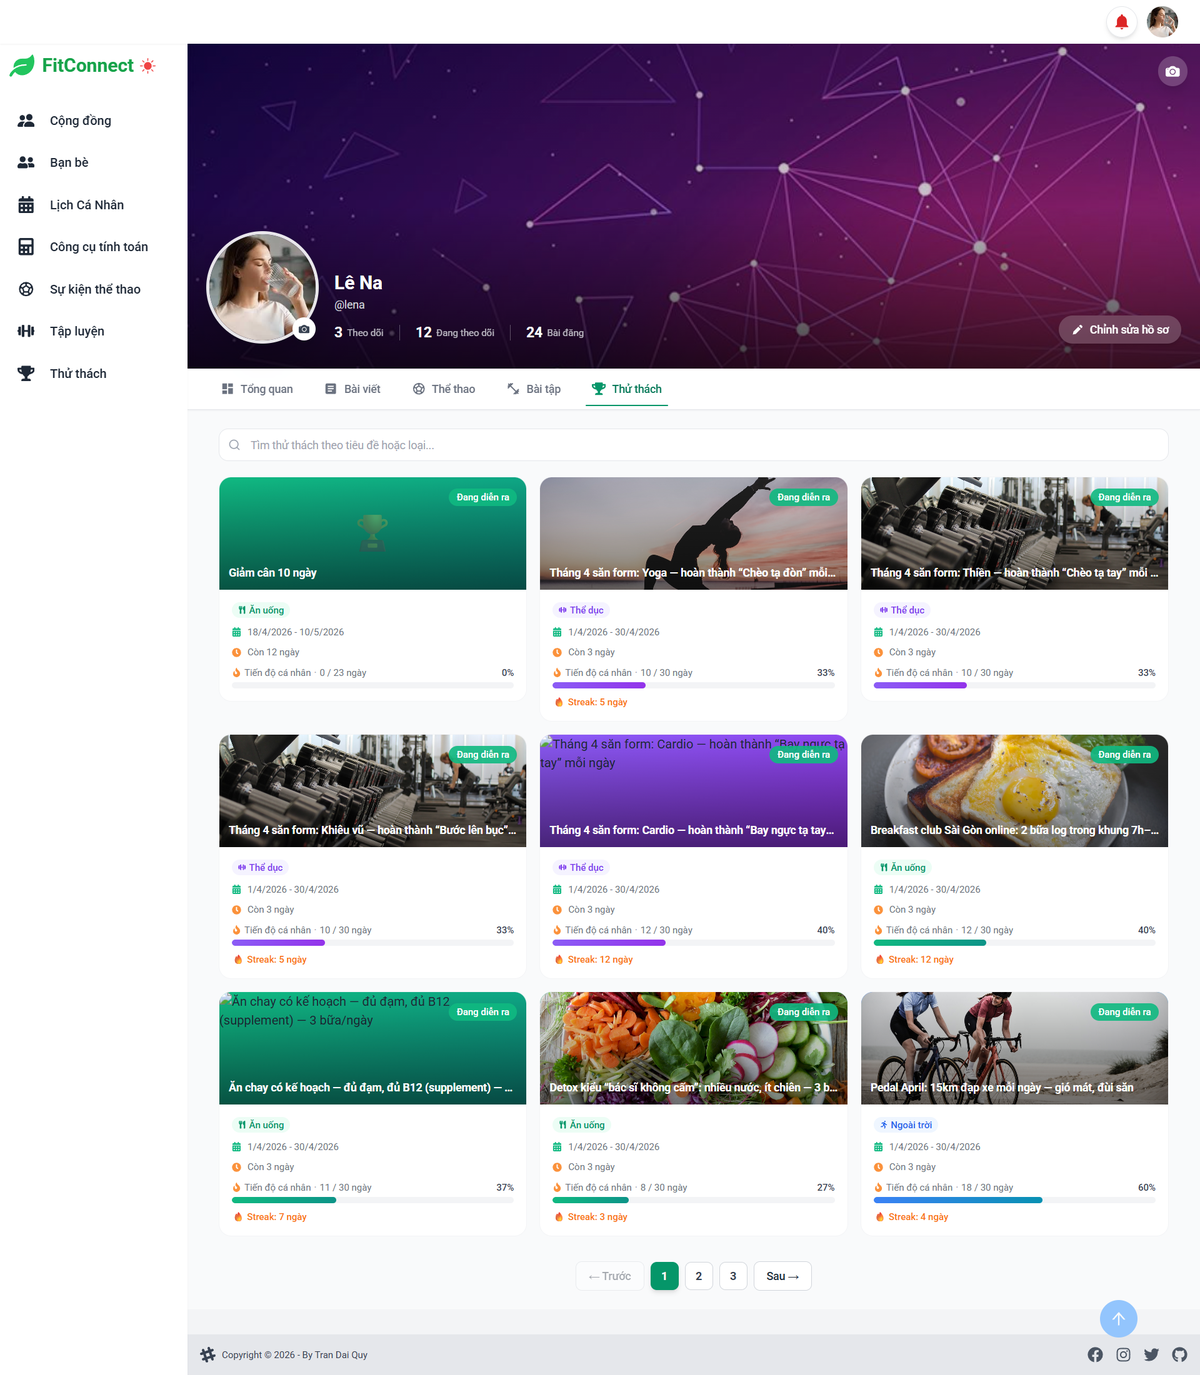
\includegraphics[width=\textwidth]{Images/IMG/Nhom1/tabthuthach.png}
        \caption{Tab Thử thách}
        \label{fig:impl_profile_challenges_tab}
    \end{subfigure}
    \vspace{0.3em}
    \caption{Ba tab theo dõi hoạt động trên trang cá nhân Profile Dashboard}
    \label{fig:impl_profile_tabs}
\end{figure}


    \item Để cá nhân hóa giao diện hồ sơ, người dùng có thể thay đổi ảnh đại diện và ảnh nền thông qua các modal thao tác nhanh. Cơ chế này cho phép cập nhật trực tiếp trên trang cá nhân mà không cần chuyển trang.

\begin{figure}[H]
    \centering
    \begin{subfigure}[b]{0.47\textwidth}
        \centering
        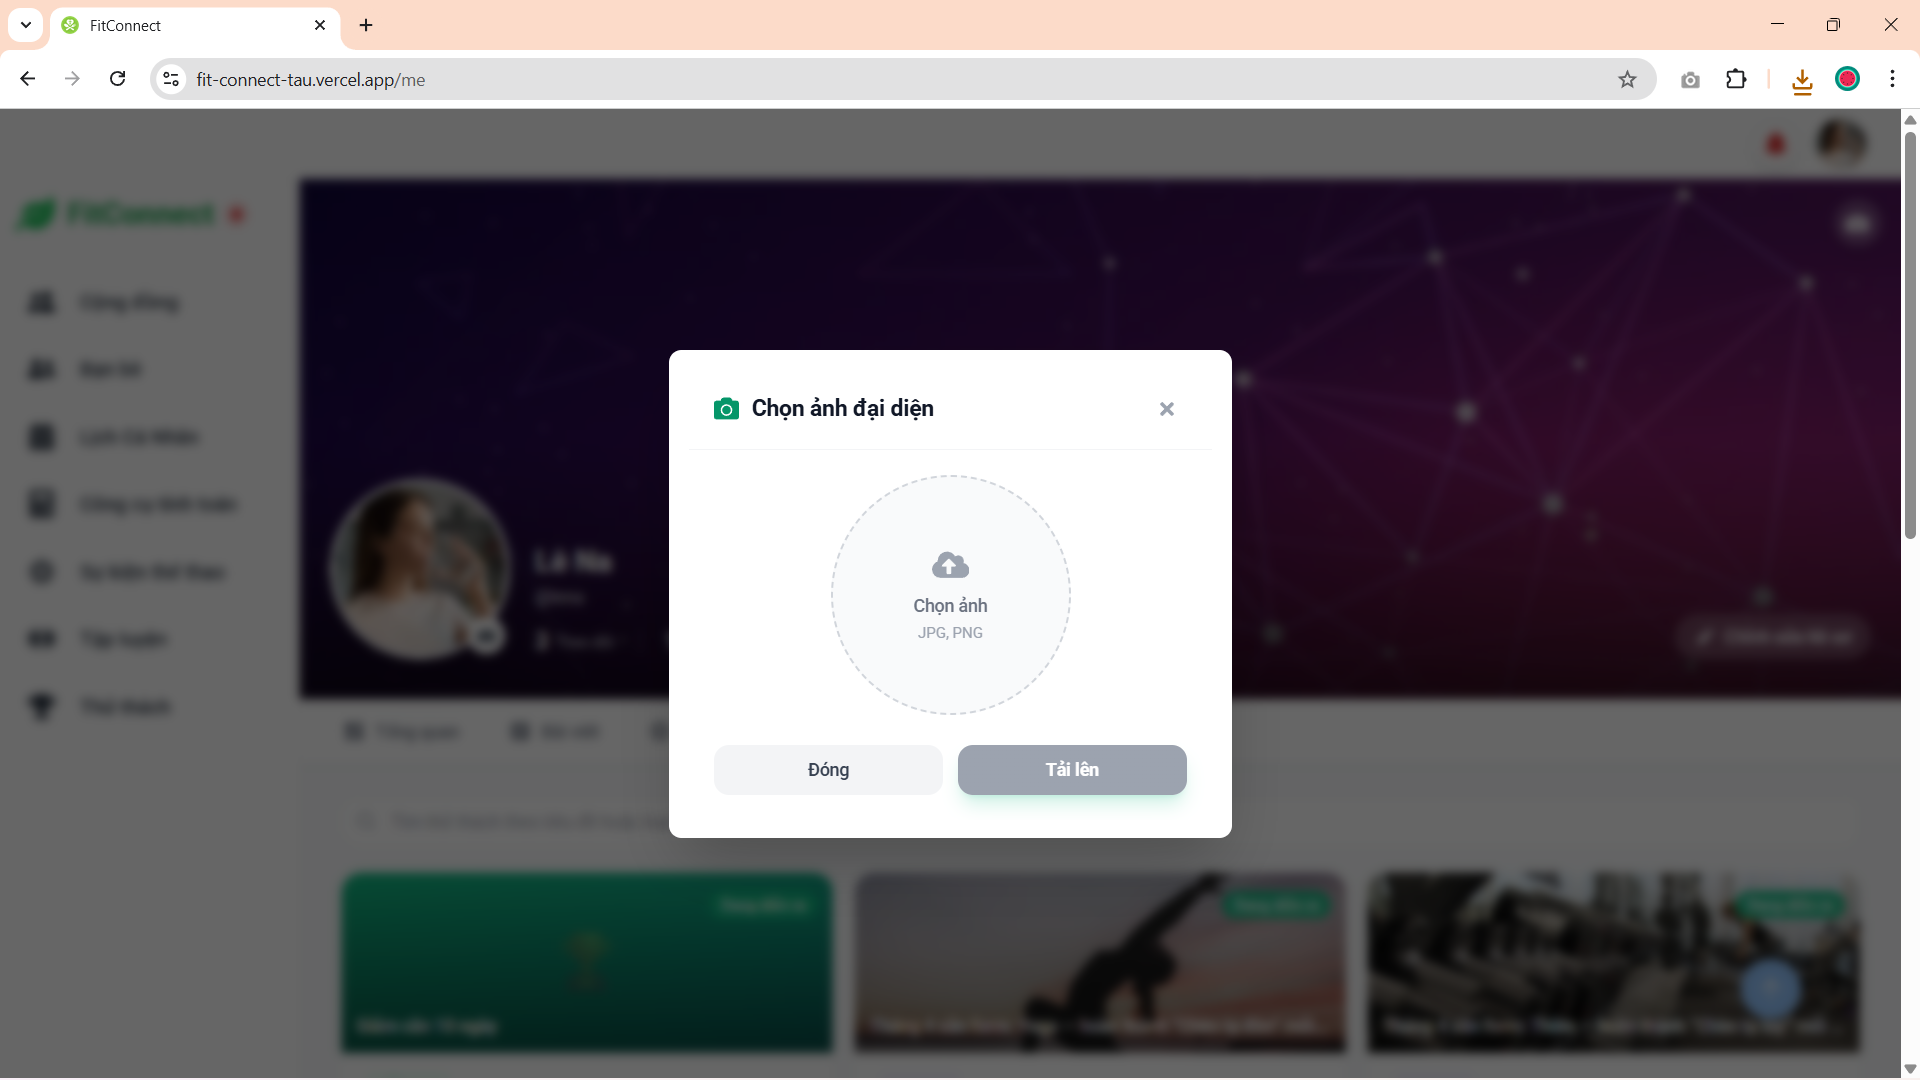
\includegraphics[width=\textwidth]{Images/IMG/Nhom1/modaldoiavatar.png}
        \caption{Modal thay đổi ảnh đại diện trên trang cá nhân}
        \label{fig:impl_profile_avatar_modal}
    \end{subfigure}
    \hfill
    \begin{subfigure}[b]{0.47\textwidth}
        \centering
        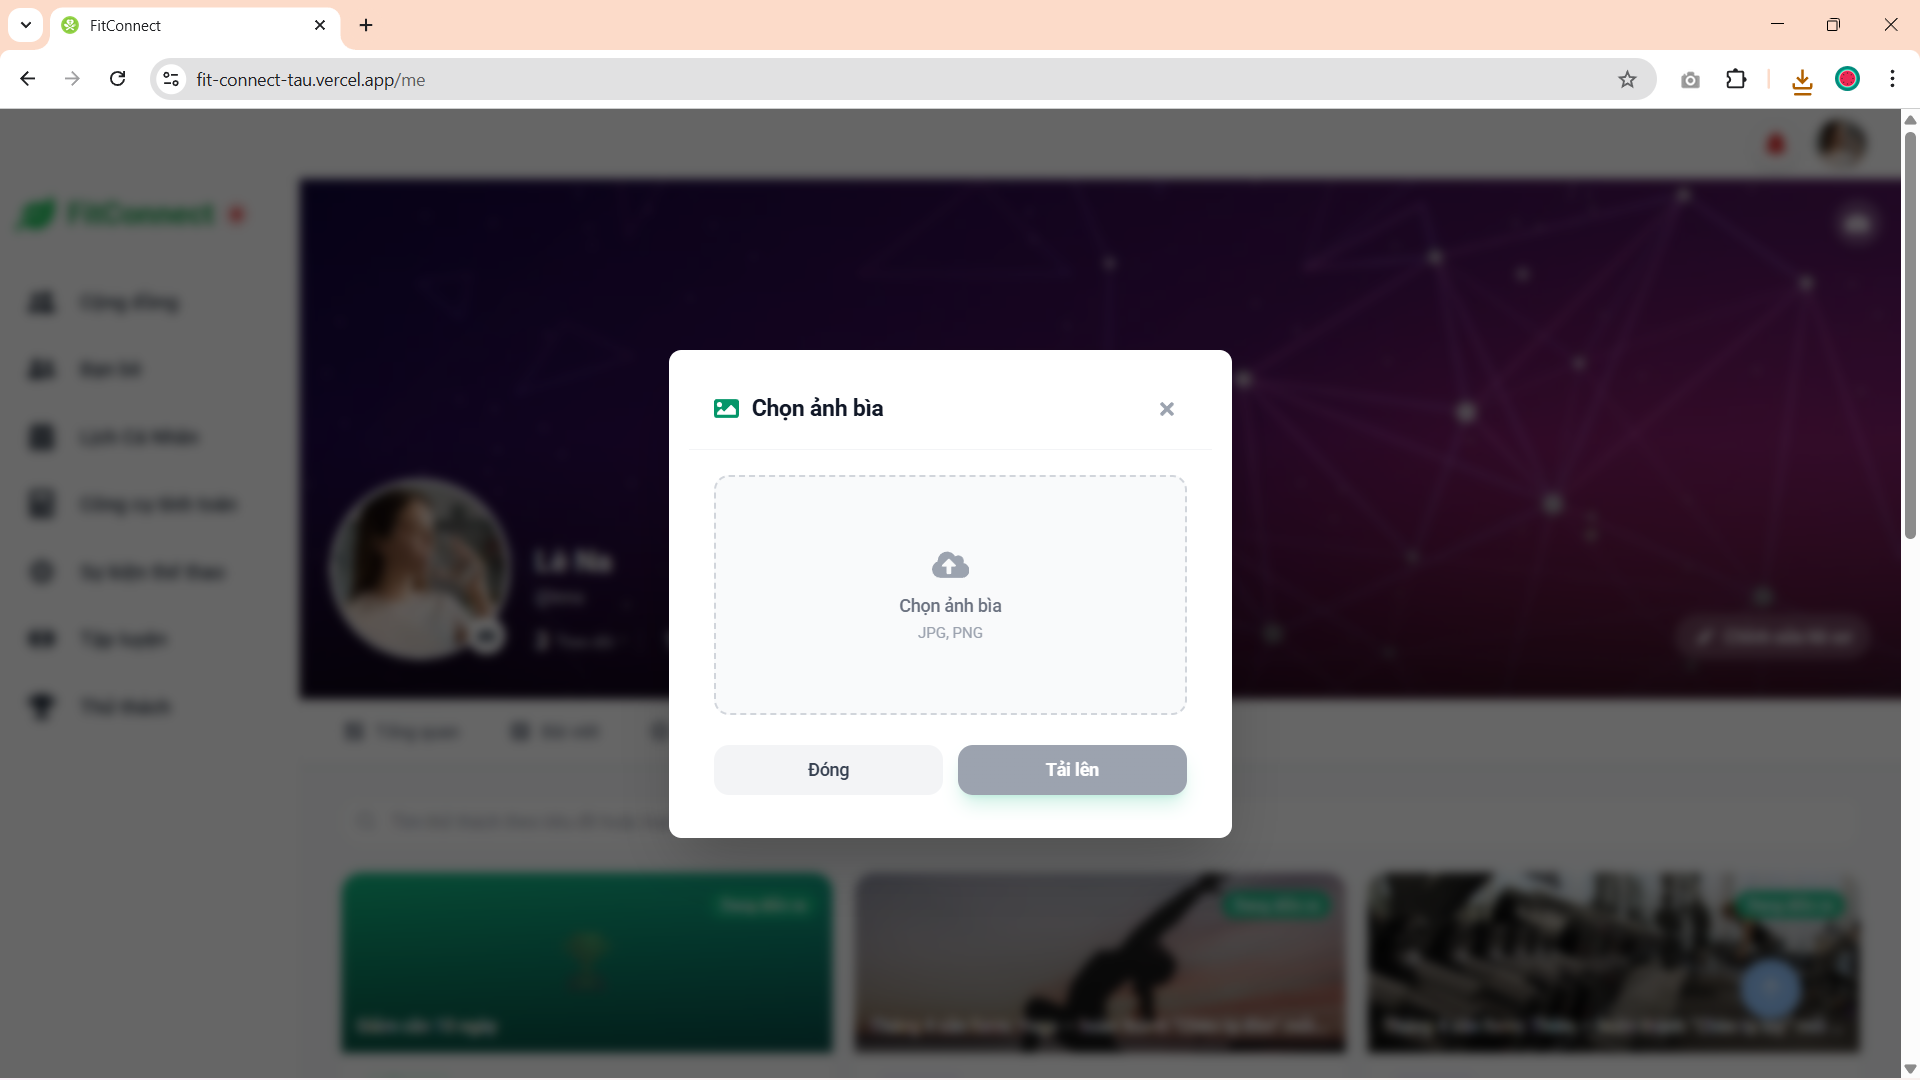
\includegraphics[width=\textwidth]{Images/IMG/Nhom1/modaldoibackgroud.png}
        \caption{Modal thay đổi ảnh nền trang cá nhân}
        \label{fig:impl_profile_cover_modal}
    \end{subfigure}
\end{figure}


    \item Ngoài phần hiển thị, người dùng có thể cập nhật thông tin hồ sơ (thông tin cá nhân và nhân trắc học) và thay đổi mật khẩu để tăng cường quản trị tài khoản, bảo đảm tính chính xác dữ liệu và an toàn truy cập.

\begin{figure}[H]
    \centering
    \begin{subfigure}[b]{0.47\textwidth}
        \centering
        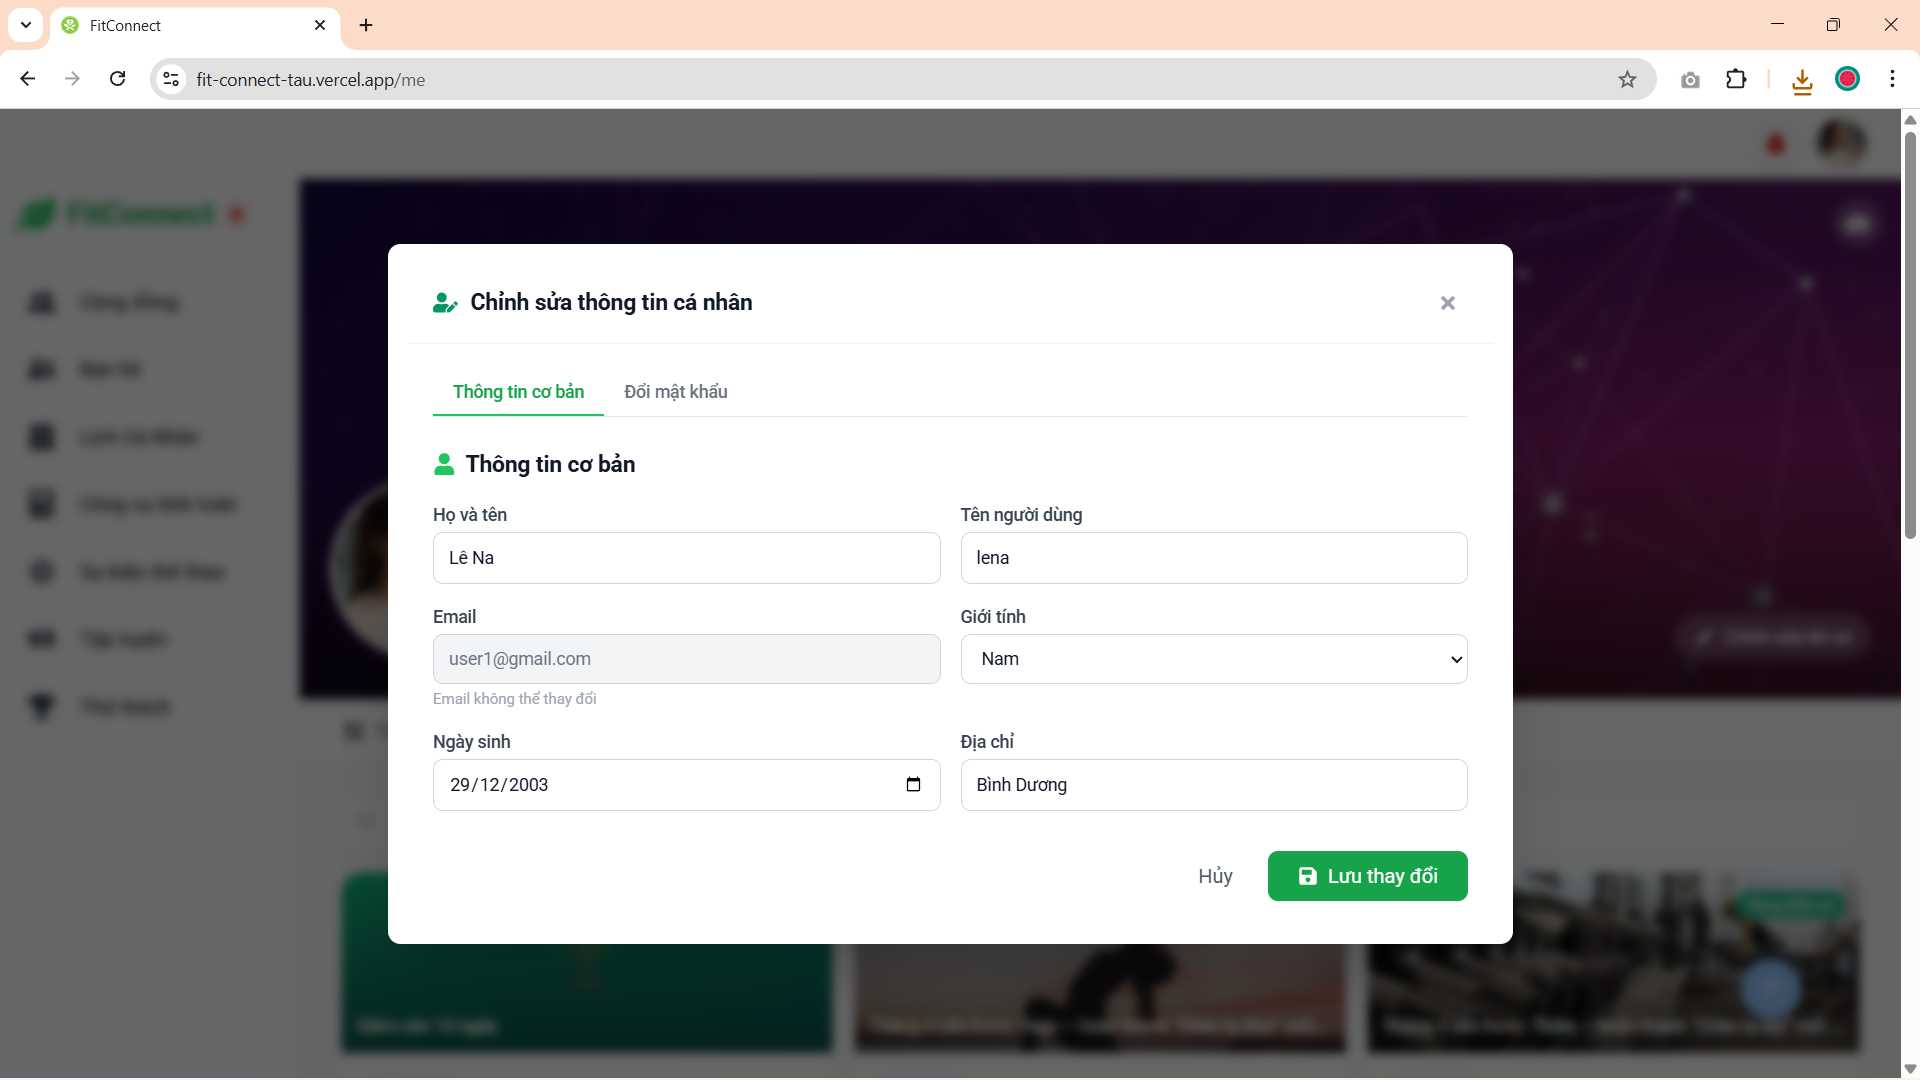
\includegraphics[width=\textwidth]{Images/IMG/Nhom1/capnhatthongtin.png}
        \caption{Người dùng cập nhật thông tin hồ sơ cá nhân}
        \label{fig:impl_profile_update}
    \end{subfigure}
    \hfill
    \begin{subfigure}[b]{0.47\textwidth}
        \centering
        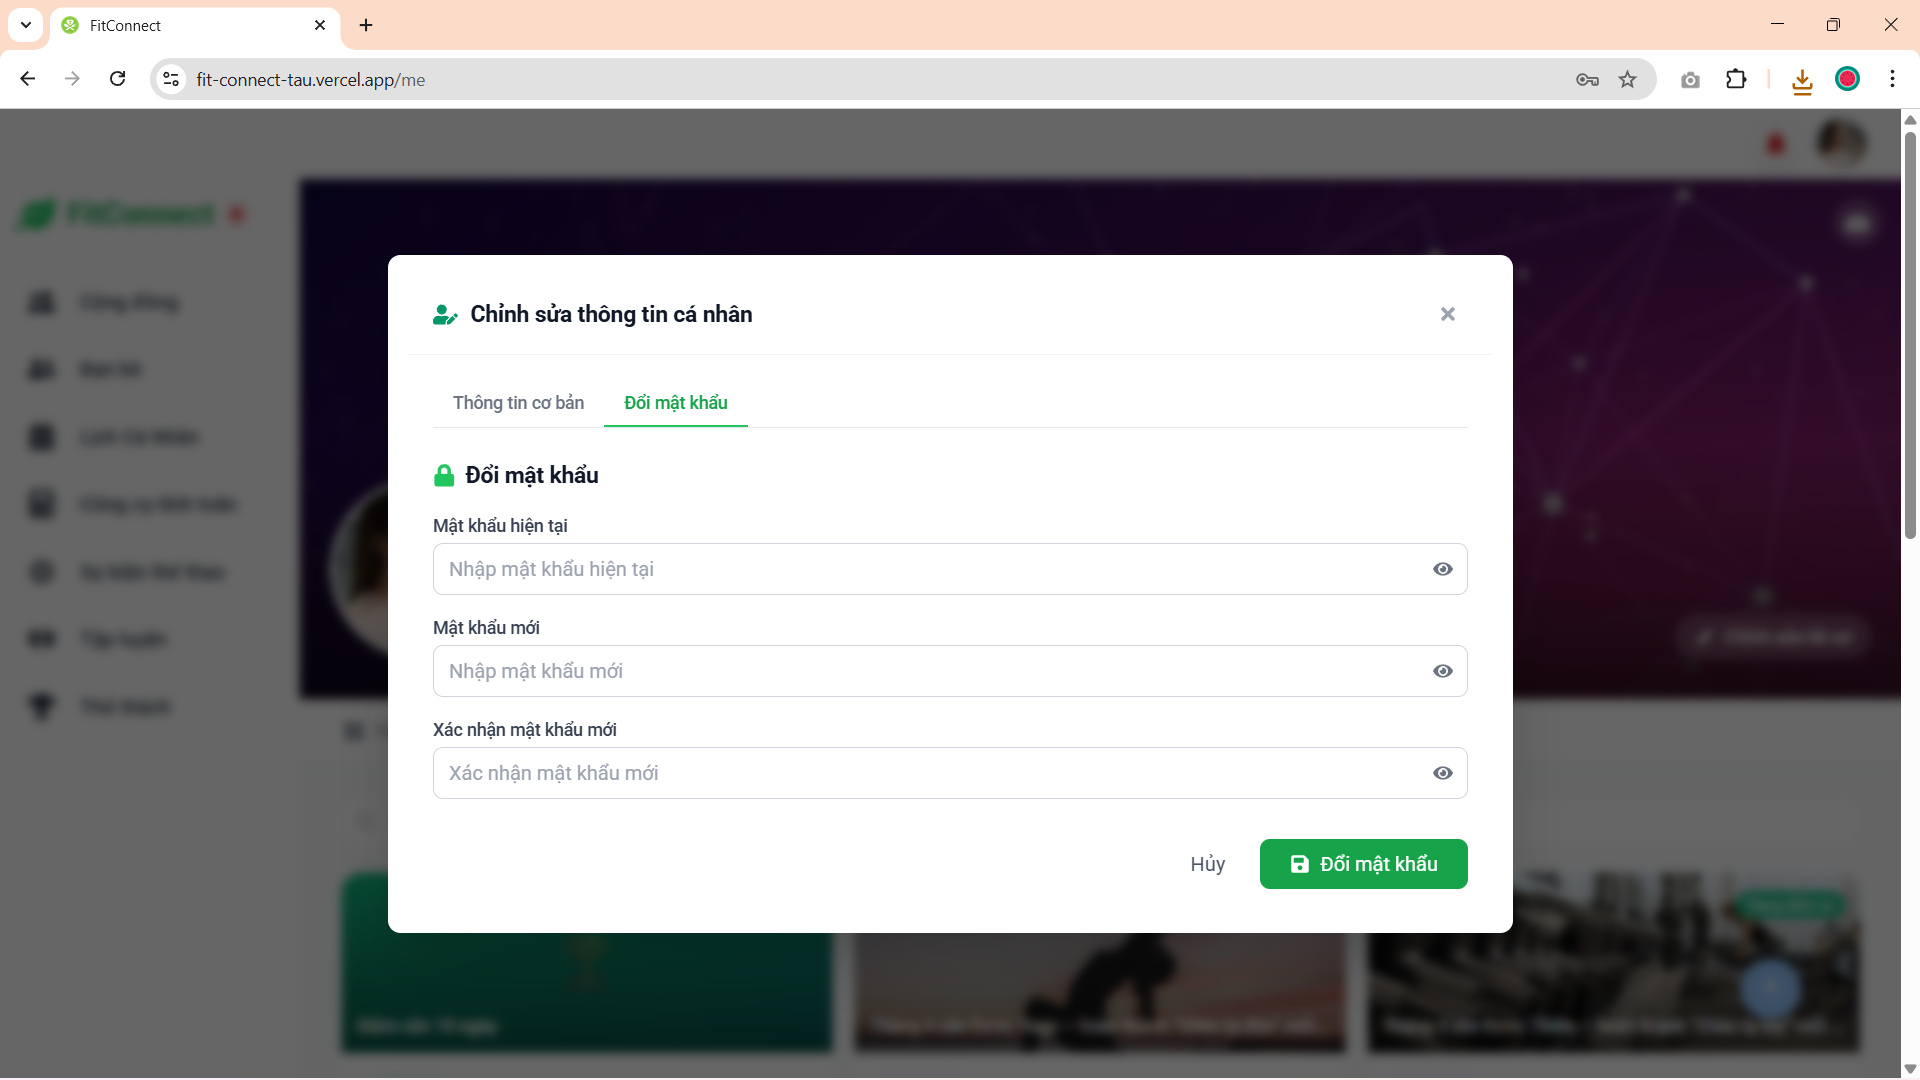
\includegraphics[width=\textwidth]{Images/IMG/Nhom1/capnhatmatkhau.png}
        \caption{Người dùng cập nhật mật khẩu trong khu vực quản trị hồ sơ}
        \label{fig:impl_profile_change_password}
    \end{subfigure}
\end{figure}

\end{itemize}


\subsection{Nhóm tính năng Mạng xã hội cộng đồng}
\label{subsec:impl_social}

Nhóm tính năng Mạng xã hội cộng đồng đóng vai trò là cầu nối gắn kết mọi người lại với nhau, giúp họ dễ dàng kết nối, chia sẻ và tương tác với nhau thông qua những bài viết, sự kiện thể thao hay thử thách cộng đồng được chia sẻ. Đây là nơi mọi người có thể đăng tải, chia sẻ bài viết, hình ảnh, sự kiện, thử thách,... mình yêu thích cũng như theo dõi và tương tác với những người có cùng sở thích.

Sự khác biệt của hệ thống nằm ở việc mạng xã hội cộng đồng này không chỉ dừng lại ở việc cung cấp diễn đàn mạng xã hội như các nền tảng truyền thống, mà còn là một hệ sinh thái tích hợp đầy đủ và toàn diện tính năng của mạng xã hội kết hợp với tính năng quản trị nội dung bài viết giúp mọi nội dung bài viết mà mọi người tiếp cận luôn trong sạch, lành mạnh và giúp kịp thời phát hiện xử lý những nội dung không lành mạnh với sự chung tay từ phía người dùng và quản trị viên.

Quy trình hoạt động gồm hai luồng chính:
\begin{itemize}
    \item \textbf{Người dùng:} Cho phép đăng, tương tác bài viết, báo cáo bài viết tới quản trị viên.
    \item \textbf{Quản trị viên:} Xử lý các bài viết bị báo cáo từ người dùng.
\end{itemize}

\subsubsection{Luồng thao tác Bảng tin (Góc độ Người dùng)}
\begin{itemize}
    \item Người dùng xem bảng tin bài viết Cộng đồng: Khi nhấn vào mục Cộng đồng, người dùng sẽ có thể xem được những bài viết từ cộng đồng. Hệ thống sẽ luôn cập nhật thời gian thực để giúp luôn hiển thị các bài viết mới nhất trên newfeeds của người dùng.

\begin{figure}[H]
    \centering
    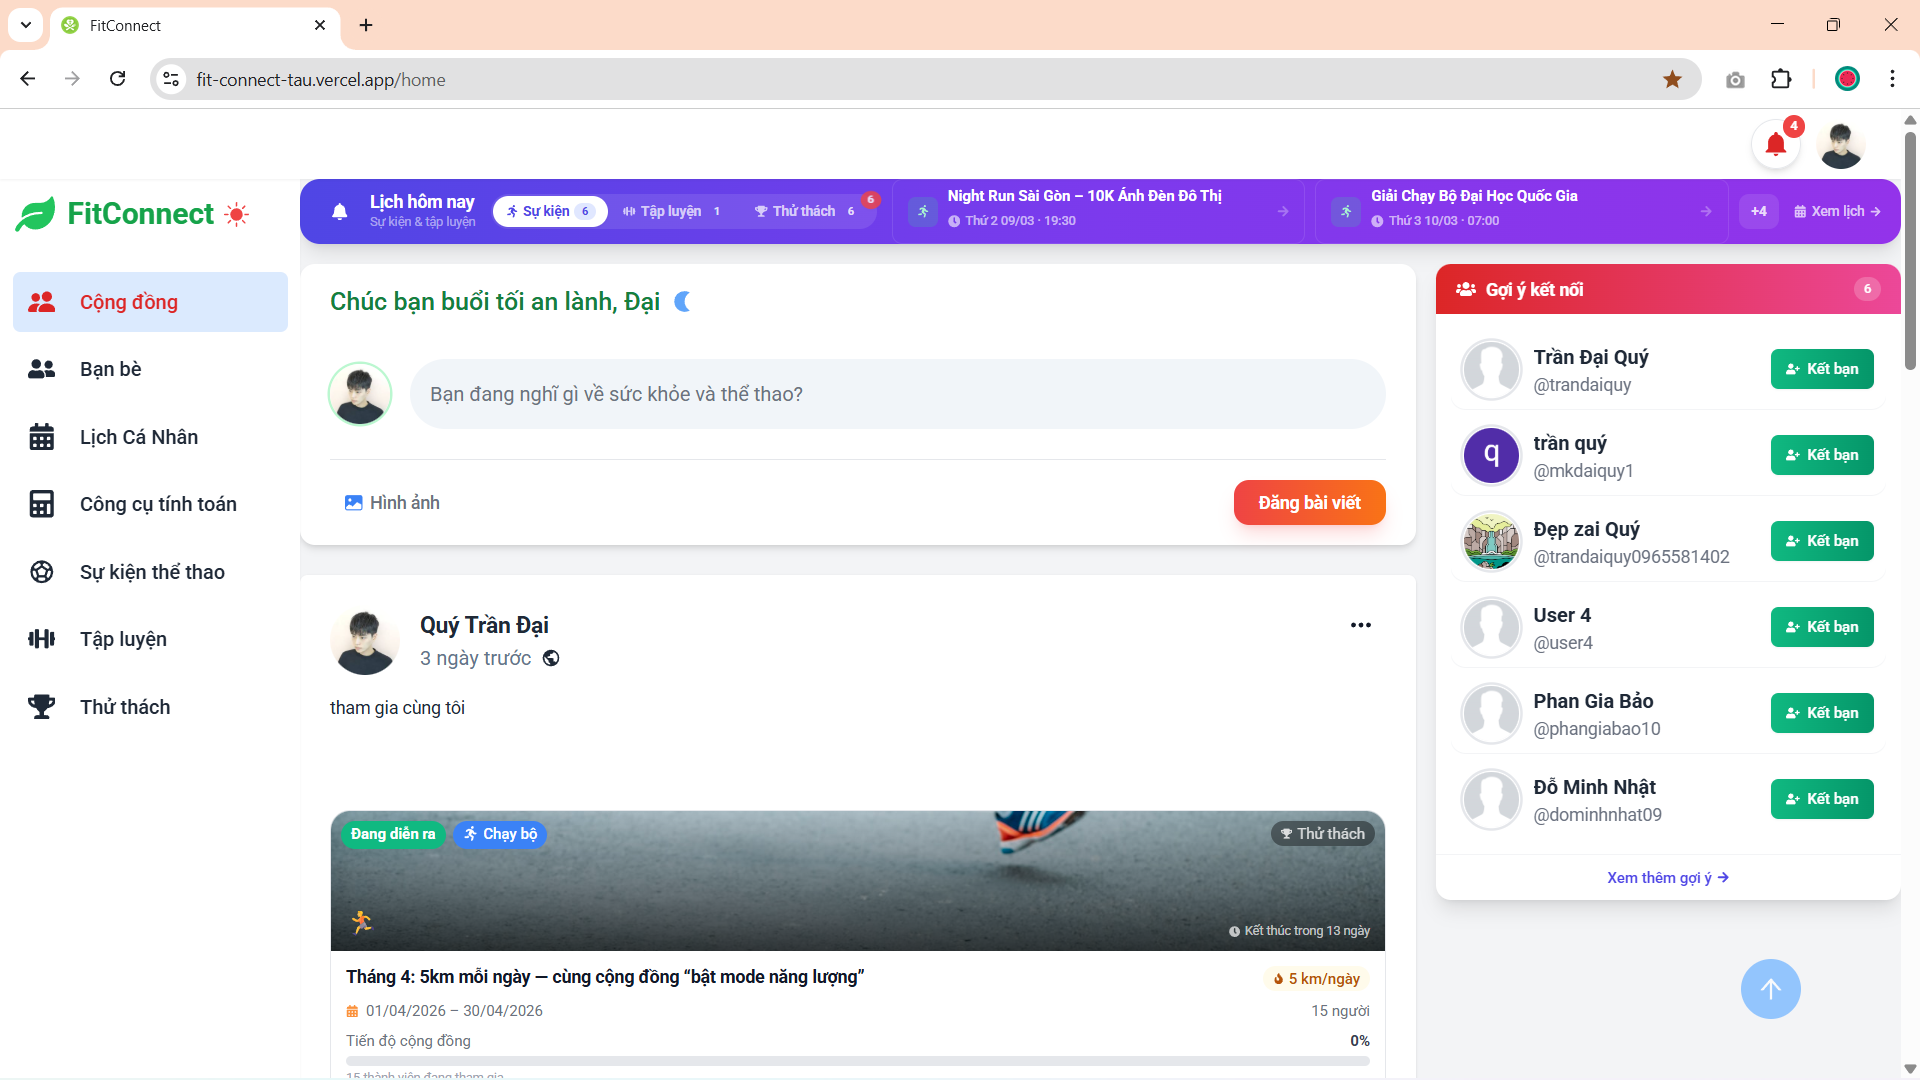
\includegraphics[width=0.60\textwidth]{Images/IMG/Nhom2/trangchucongdong.png}
    \caption{Người dùng xem trang chủ cộng đồng}
    \label{fig:impl_social_home}
\end{figure}


    \item Người dùng tạo bài viết mới: hệ thống hiển thị Modal soạn nội dung, chèn hình ảnh (tối đa 5 ảnh), đính kèm biểu tượng cảm xúc và chọn đối tượng hướng đến. Khi nhấn Đăng, AI tự động kiểm tra hình ảnh: nếu phát hiện nội dung nhạy cảm, bài viết bị chặn với cảnh báo; nếu hợp lệ, bài viết được đăng và bảng tin tự động làm mới.

\begin{figure}[H]
    \centering
    \begin{subfigure}[b]{0.47\textwidth}
        \centering
        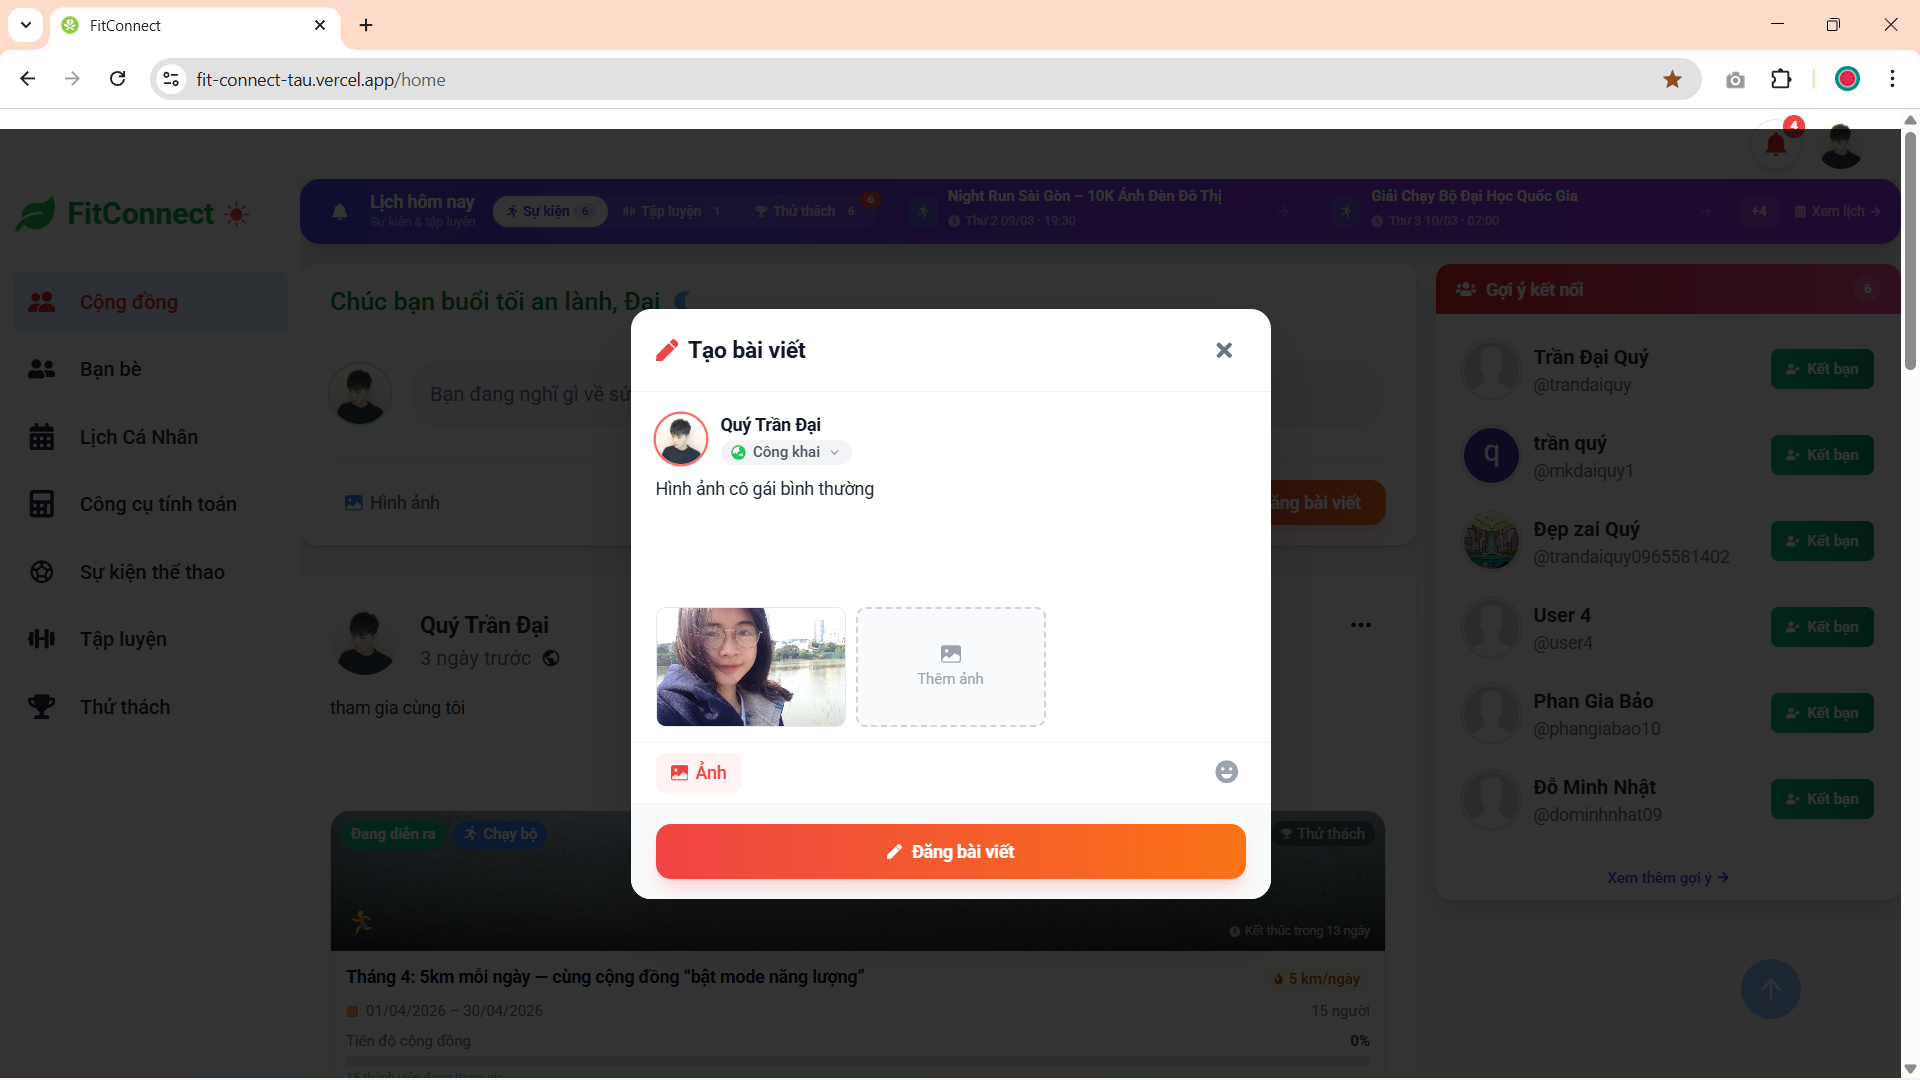
\includegraphics[width=\textwidth]{Images/IMG/Nhom2/dangbaivietbinhthuong.png}
        \caption{Modal soạn và đăng bài viết bình thường}
        \label{fig:impl_social_post}
    \end{subfigure}
    \hfill
    \begin{subfigure}[b]{0.47\textwidth}
        \centering
        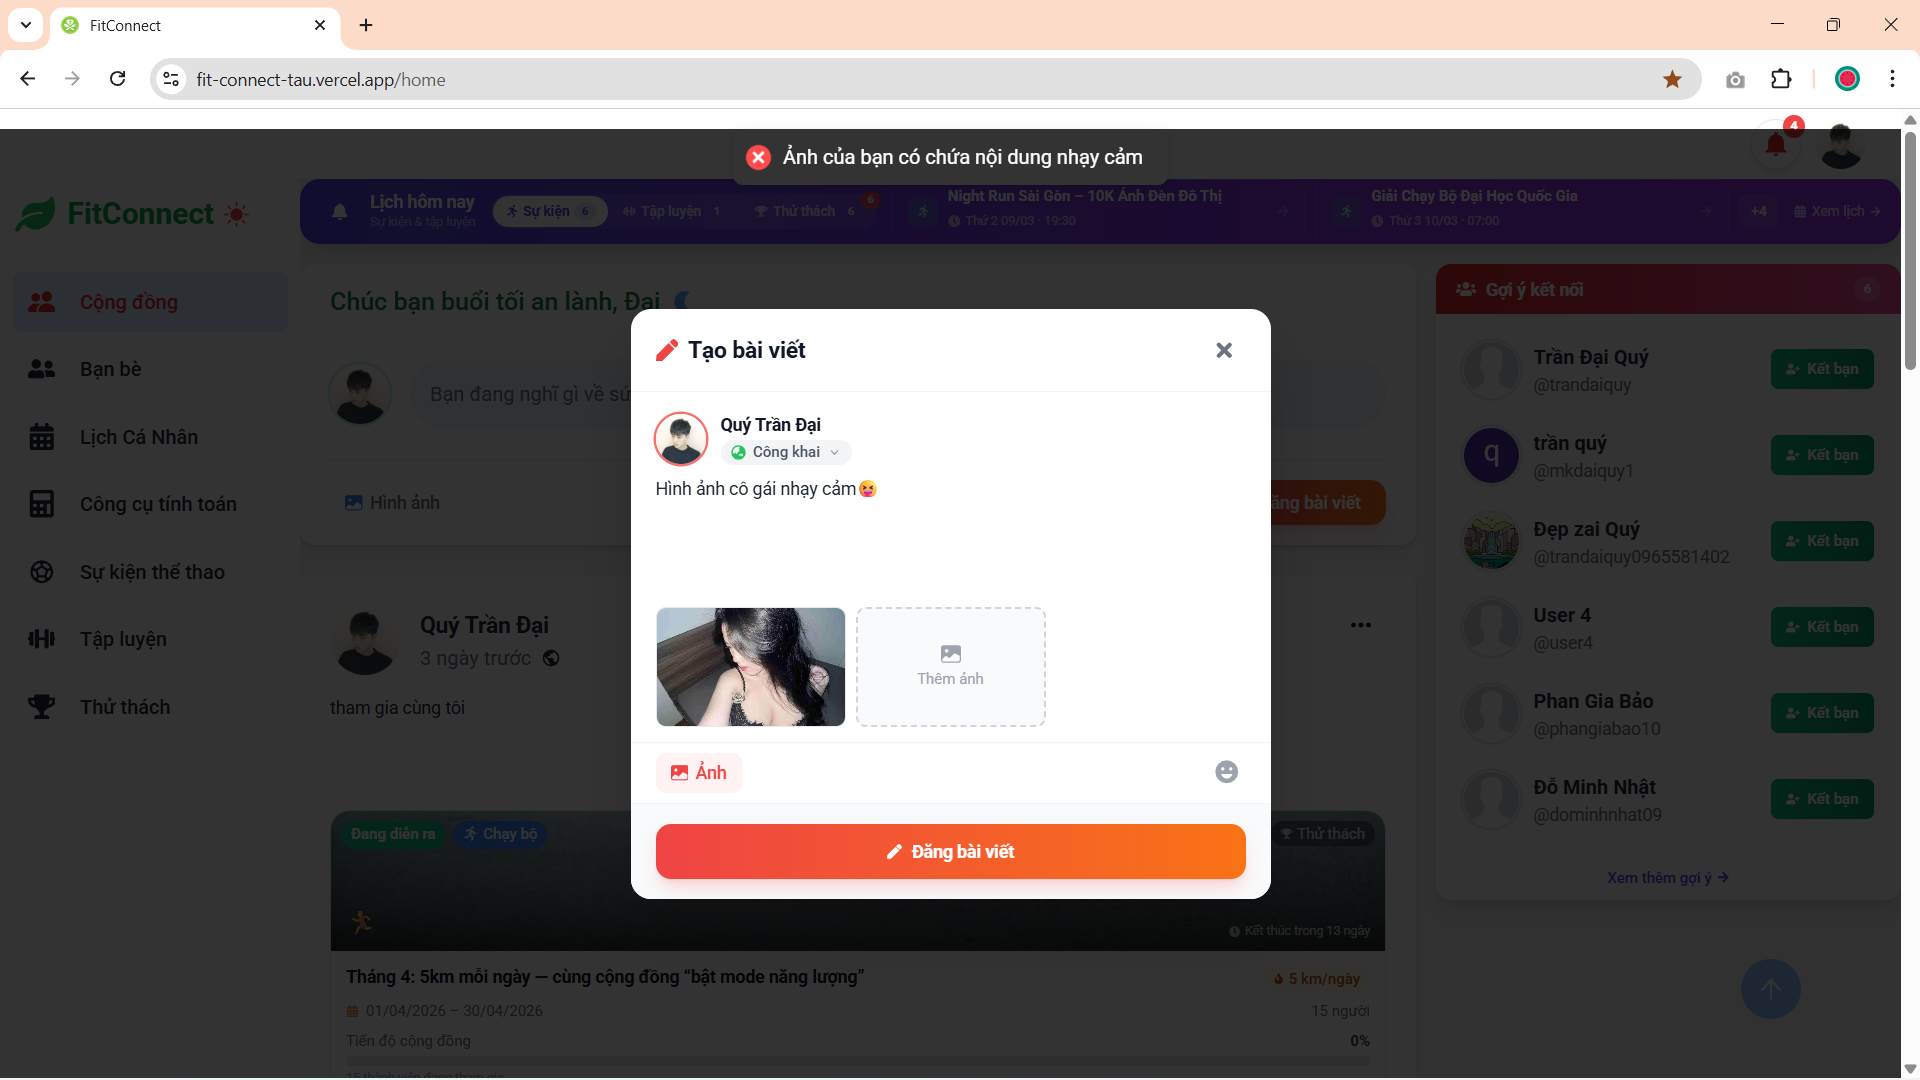
\includegraphics[width=\textwidth]{Images/IMG/Nhom2/dangbaivietchuahinhanhvipham.png}
        \caption{Hệ thống chặn đăng bài khi phát hiện hình ảnh vi phạm}
        \label{fig:impl_social_violate}
    \end{subfigure}
    \vspace{0.3em}
    \caption{Luồng đăng bài viết với kiểm duyệt AI hình ảnh tự động}
    \label{fig:impl_social_post_flow}
\end{figure}

    \item Những người dùng khác trong hệ thống có thể tương tác thích và bình luận về bài viết. Người dùng có thể trả lời những bình luận của nhau, giúp trao đổi tương tác liên tục.

\begin{figure}[H]
    \centering
    \begin{subfigure}[b]{0.47\textwidth}
        \centering
        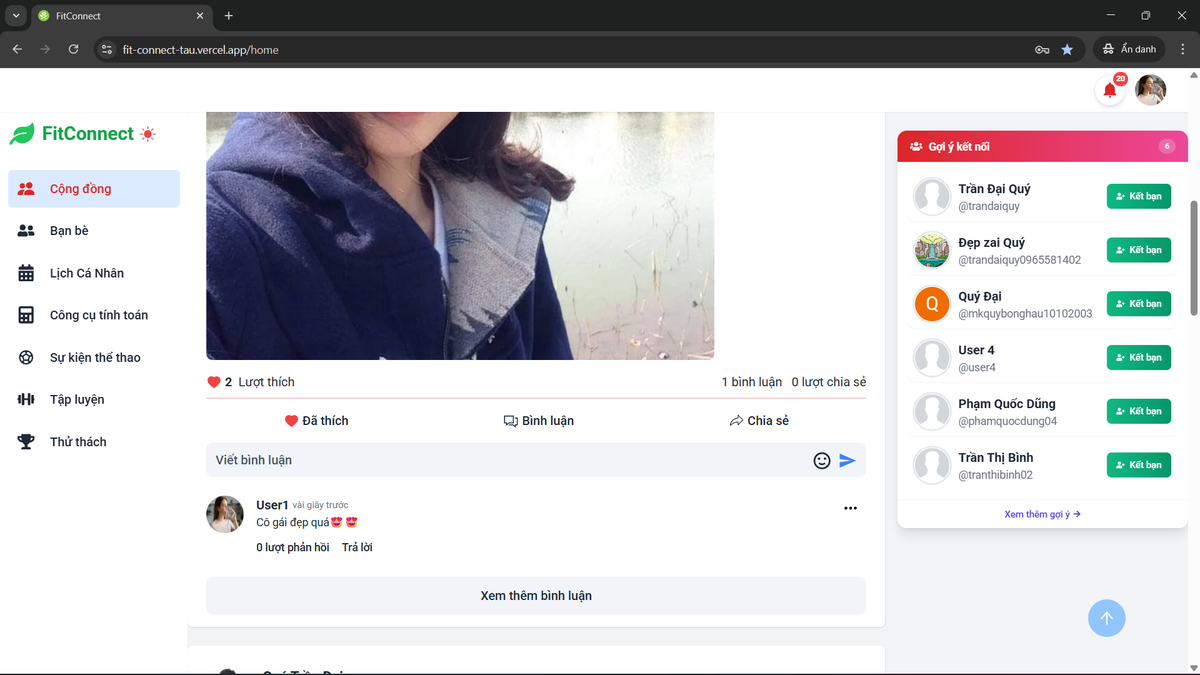
\includegraphics[width=\textwidth]{Images/IMG/Nhom2/nguoikhacthichvabinhluan.png}
        \caption{Người dùng nhận thông báo khi người khác thích và bình luận}
        \label{fig:impl_social_interact}
    \end{subfigure}
    \hfill
    \begin{subfigure}[b]{0.47\textwidth}
        \centering
        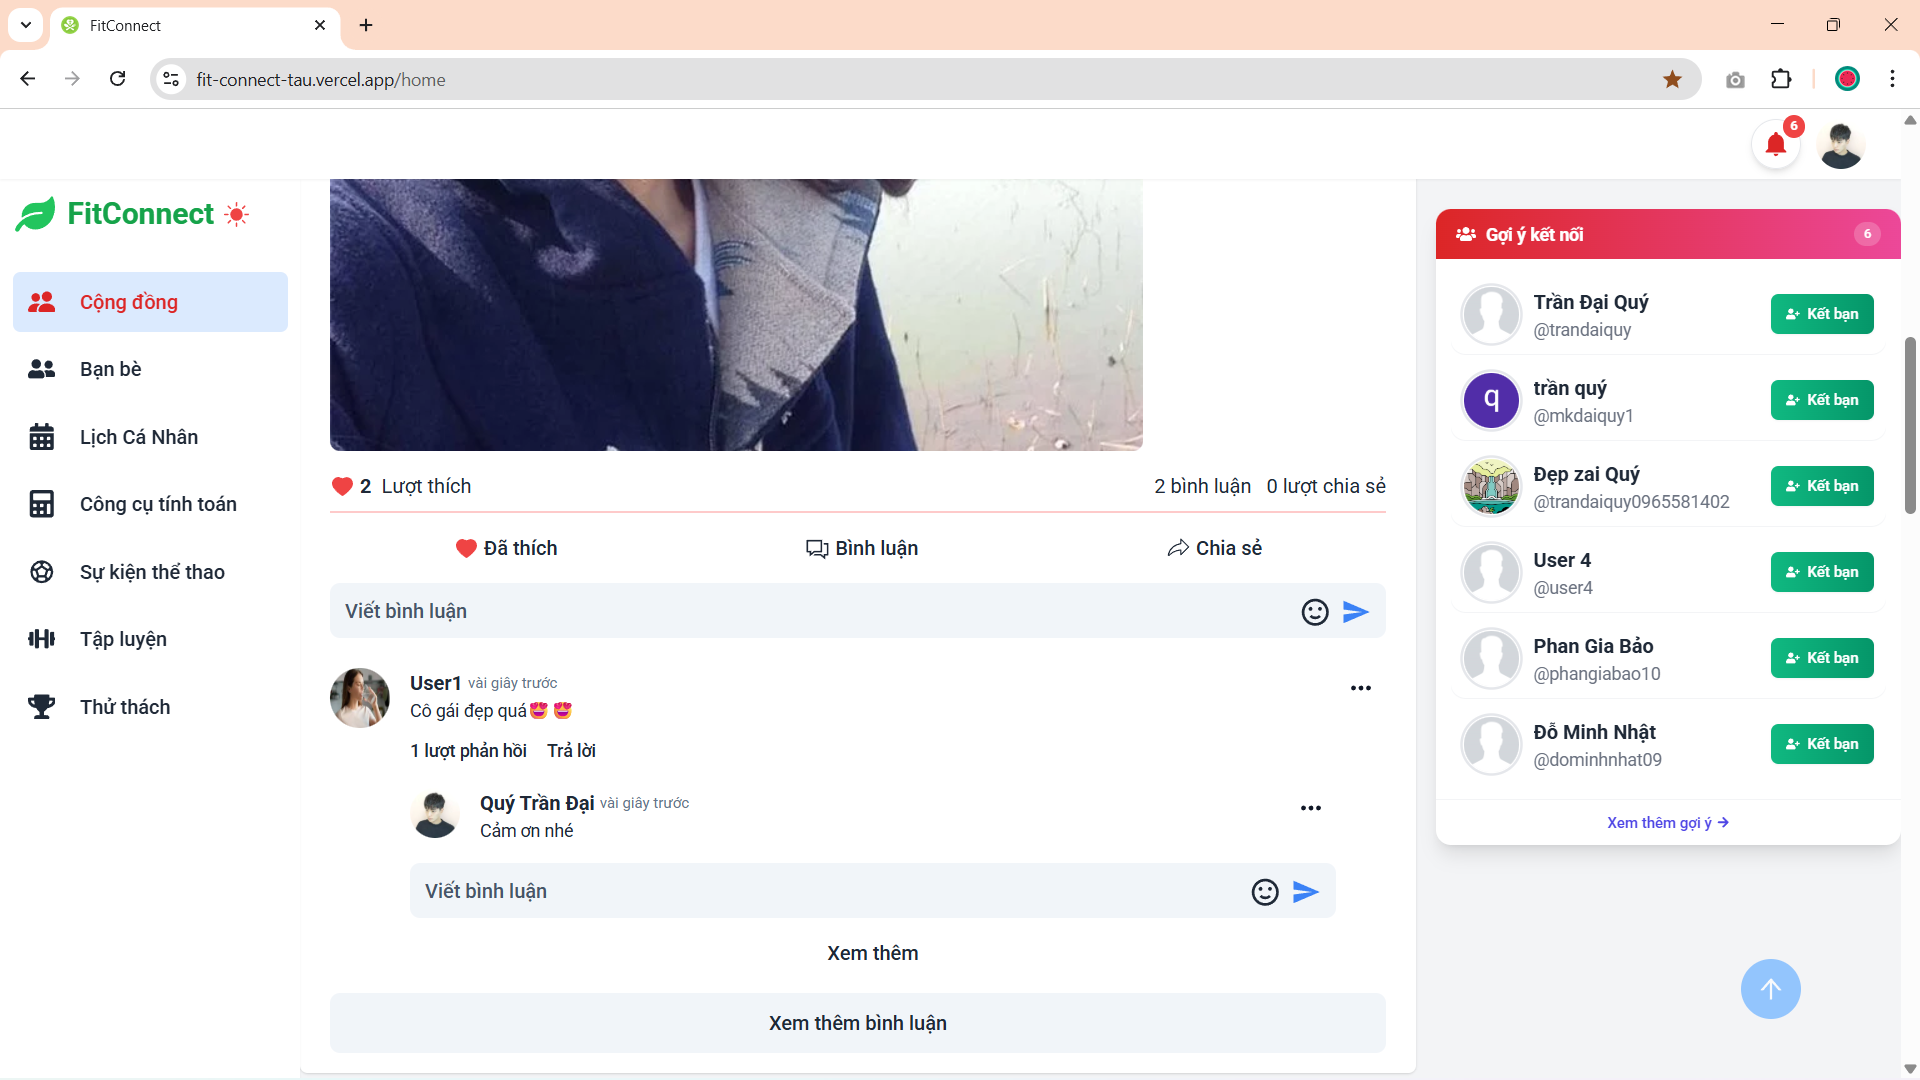
\includegraphics[width=\textwidth]{Images/IMG/Nhom2/traloibinhluannguoido.png}
        \caption{Người dùng thao tác trả lời bình luận người đó}
        \label{fig:impl_social_reply}
    \end{subfigure}
\end{figure}


    \item Người dùng có thể chia sẻ bài viết của người khác về Bảng tin của mình hoặc tự xóa bài viết của mình khi không còn phù hợp.

\begin{figure}[H]
    \centering
    \begin{subfigure}[b]{0.47\textwidth}
        \centering
        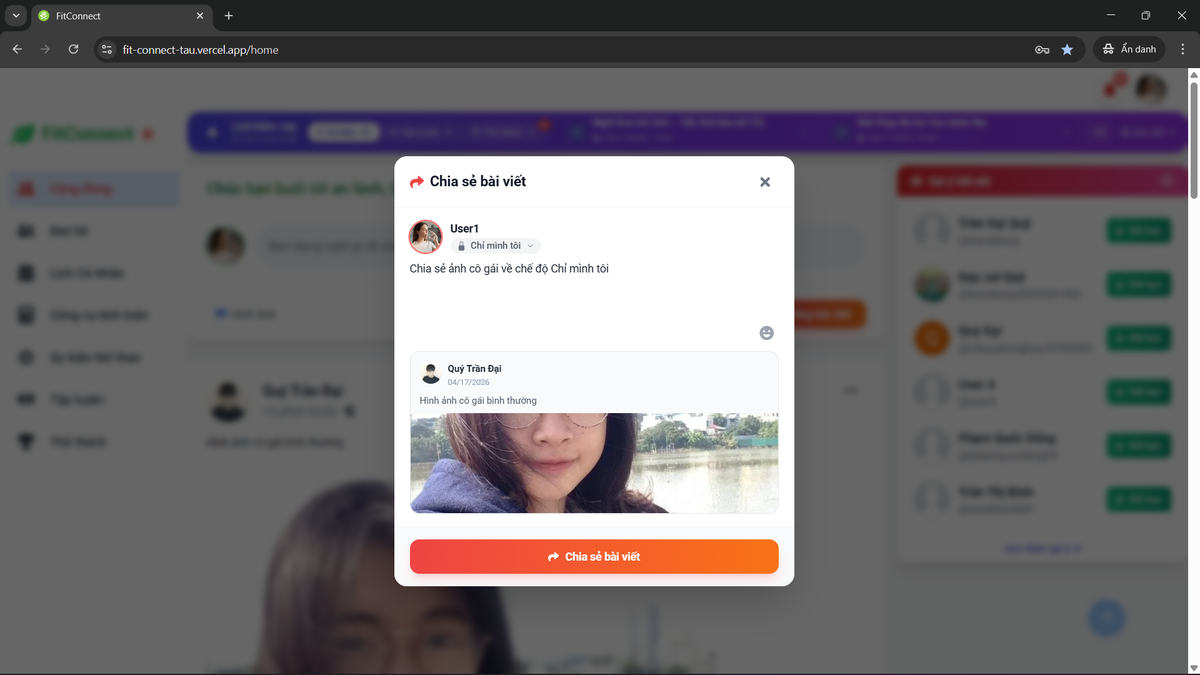
\includegraphics[width=\textwidth]{Images/IMG/Nhom2/chiasebaivietnguoikhac.png}
        \caption{Thao tác chia sẻ bài viết lên Bảng tin}
        \label{fig:impl_social_share}
    \end{subfigure}
    \hfill
    \begin{subfigure}[b]{0.47\textwidth}
        \centering
        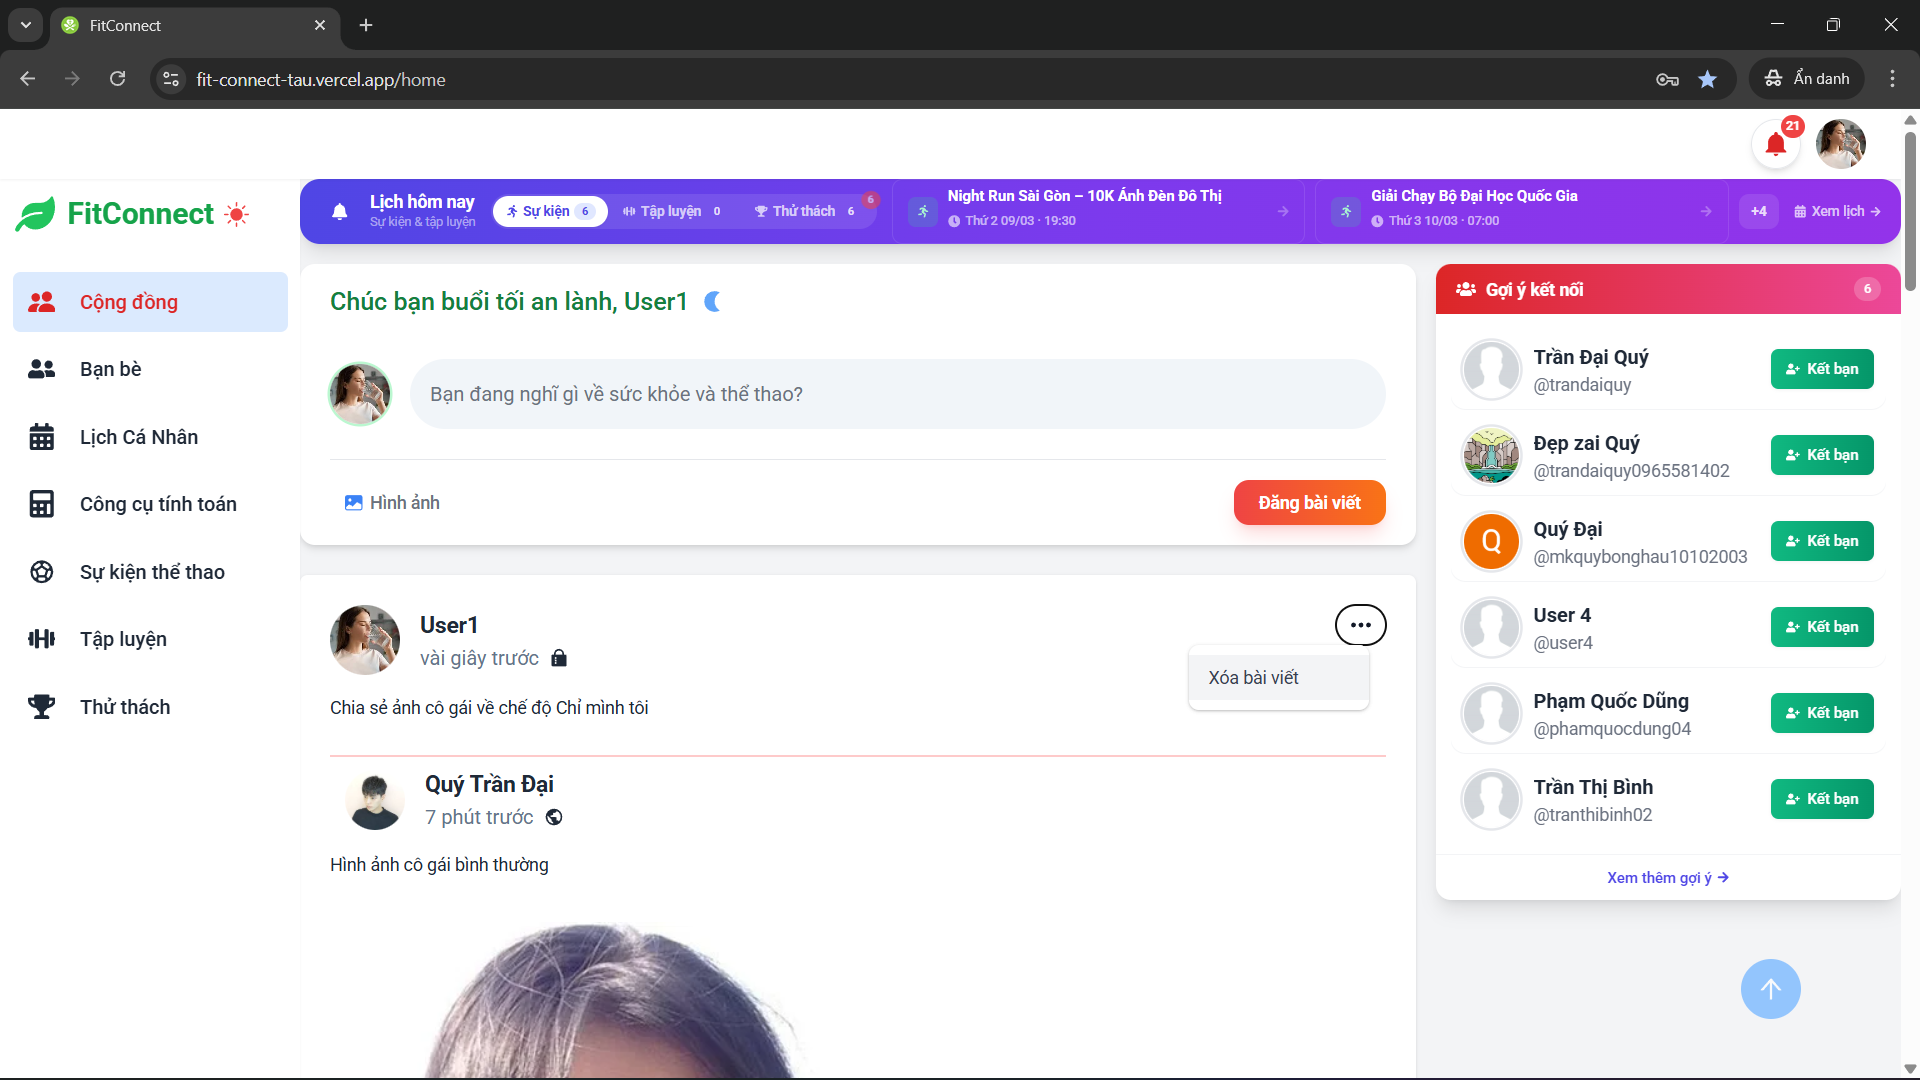
\includegraphics[width=\textwidth]{Images/IMG/Nhom2/xoabaiviet.png}
        \caption{Thao tác tự xóa bài viết của mình}
        \label{fig:impl_social_delete_own}
    \end{subfigure}
    \vspace{0.3em}
    \caption{Chia sẻ và xóa bài viết trên Bảng tin cộng đồng}
    \label{fig:impl_social_share_delete}
\end{figure}


    \item Người dùng có thể báo cáo những bài viết không hợp lệ lên quản trị viên. Khi đó người bị báo cáo sẽ nhận thông báo bài viết bị báo cáo.

\begin{figure}[H]
    \centering
    \begin{subfigure}[b]{0.47\textwidth}
        \centering
        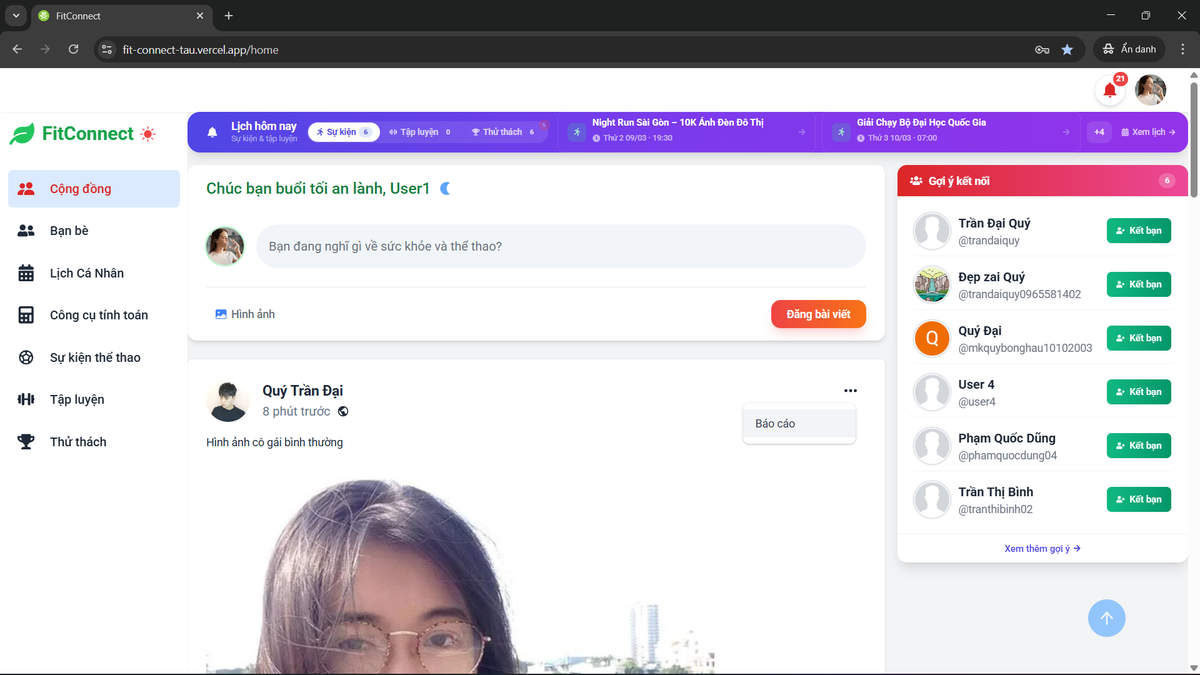
\includegraphics[width=\textwidth]{Images/IMG/Nhom2/baocaobaivietnguoikhac.png}
        \caption{Người dùng thao tác báo cáo bài viết người khác}
        \label{fig:impl_social_report}
    \end{subfigure}
    \hfill
    \begin{subfigure}[b]{0.47\textwidth}
        \centering
        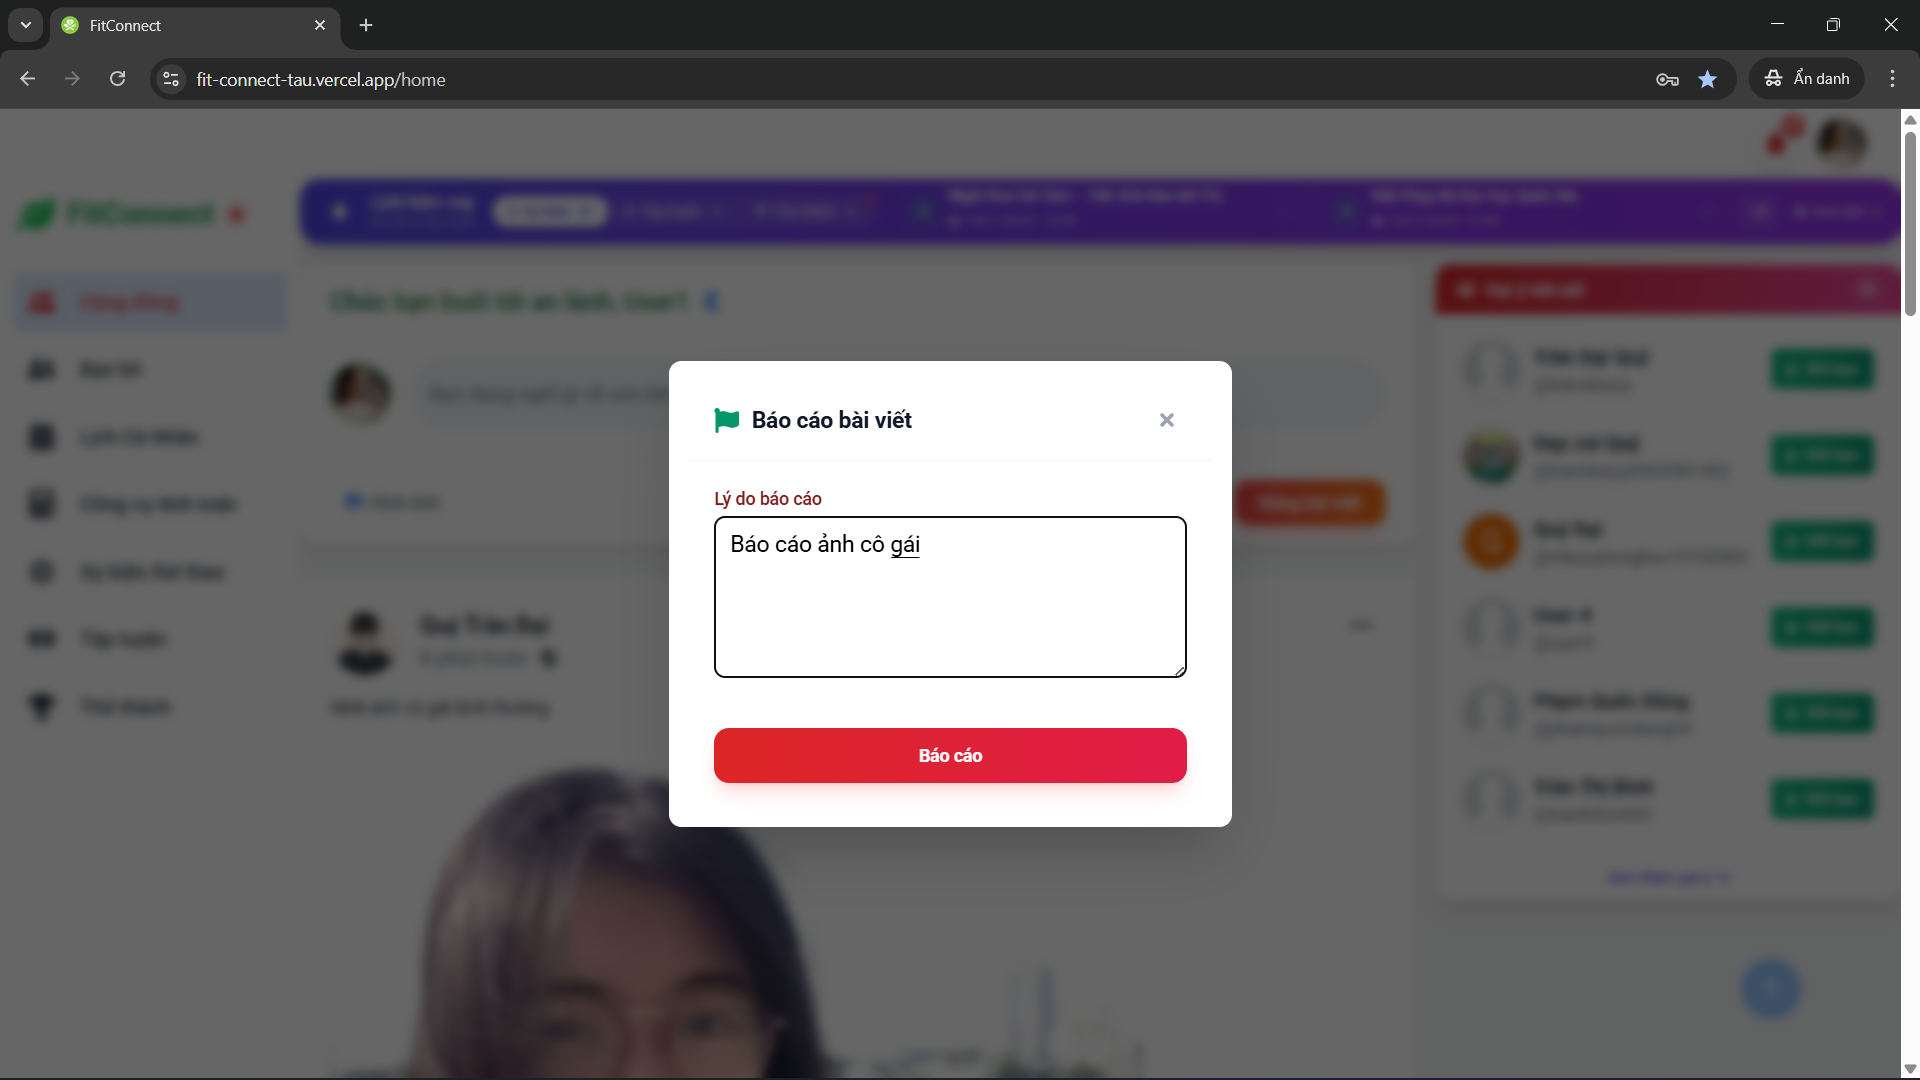
\includegraphics[width=\textwidth]{Images/IMG/Nhom2/modaldienbaocao.png}
        \caption{Hệ thống hiển thị modal tải mẫu điền báo cáo bài viết}
        \label{fig:impl_social_report_modal}
    \end{subfigure}
\end{figure}

\end{itemize}

\subsubsection{Luồng thao tác quản trị bài viết (Góc độ Quản trị viên)}
\begin{itemize}
    \item Quản trị viên xem danh sách bài viết bị báo cáo, đọc nội dung chi tiết và đưa ra quyết định: \textbf{Giữ lại} (bài viết tiếp tục hiển thị, người dùng nhận thông báo) hoặc \textbf{Xóa} (bài viết bị ẩn, chủ bài nhận thông báo vi phạm). Bài viết bị xóa được lưu trong tab ``Đã xóa'' và có thể được khôi phục nếu quản trị viên xem xét lại.

\begin{figure}[H]
    \centering
    \begin{subfigure}[b]{0.47\textwidth}
        \centering
        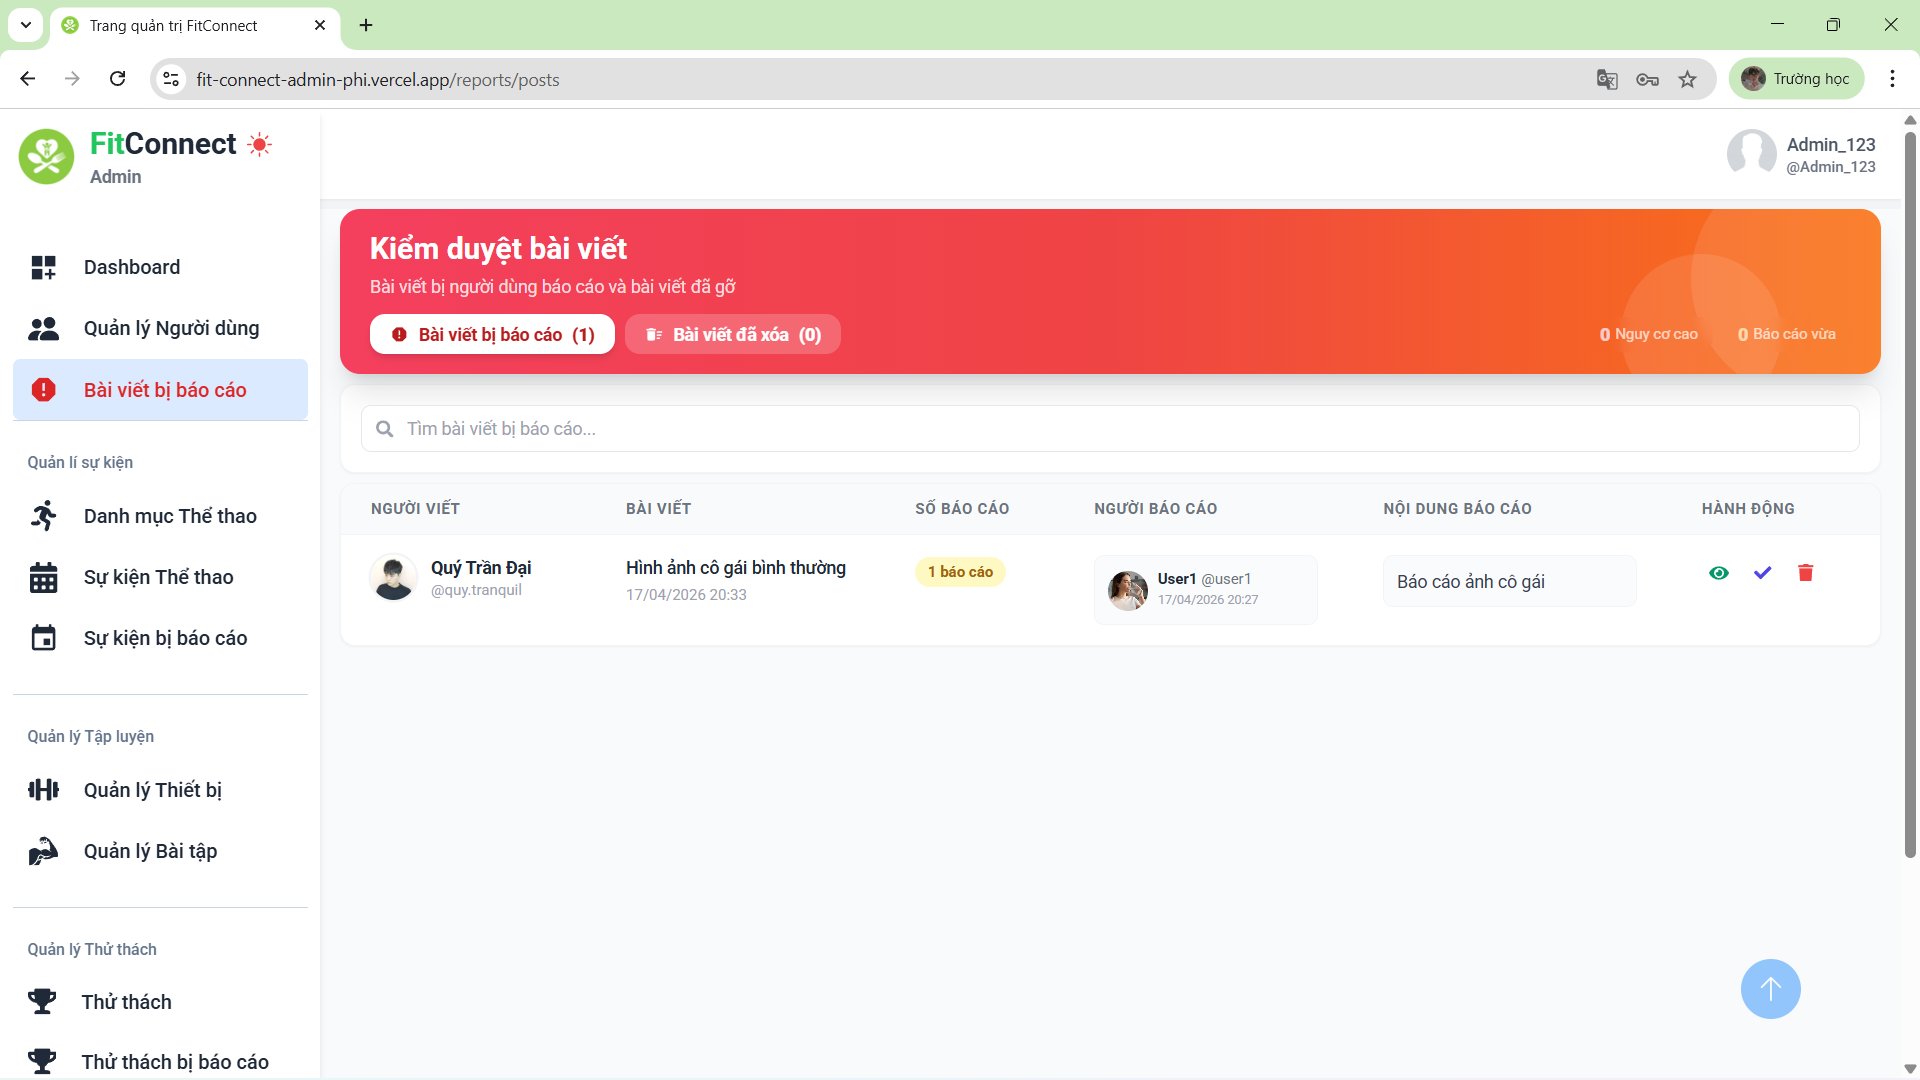
\includegraphics[width=\textwidth]{Images/IMG/Nhom2/hienbaivietbibaocaobenadmin.png}
        \caption{Danh sách bài viết bị báo cáo chờ kiểm duyệt}
        \label{fig:impl_social_admin_receive}
    \end{subfigure}
    \hfill
    \begin{subfigure}[b]{0.47\textwidth}
        \centering
        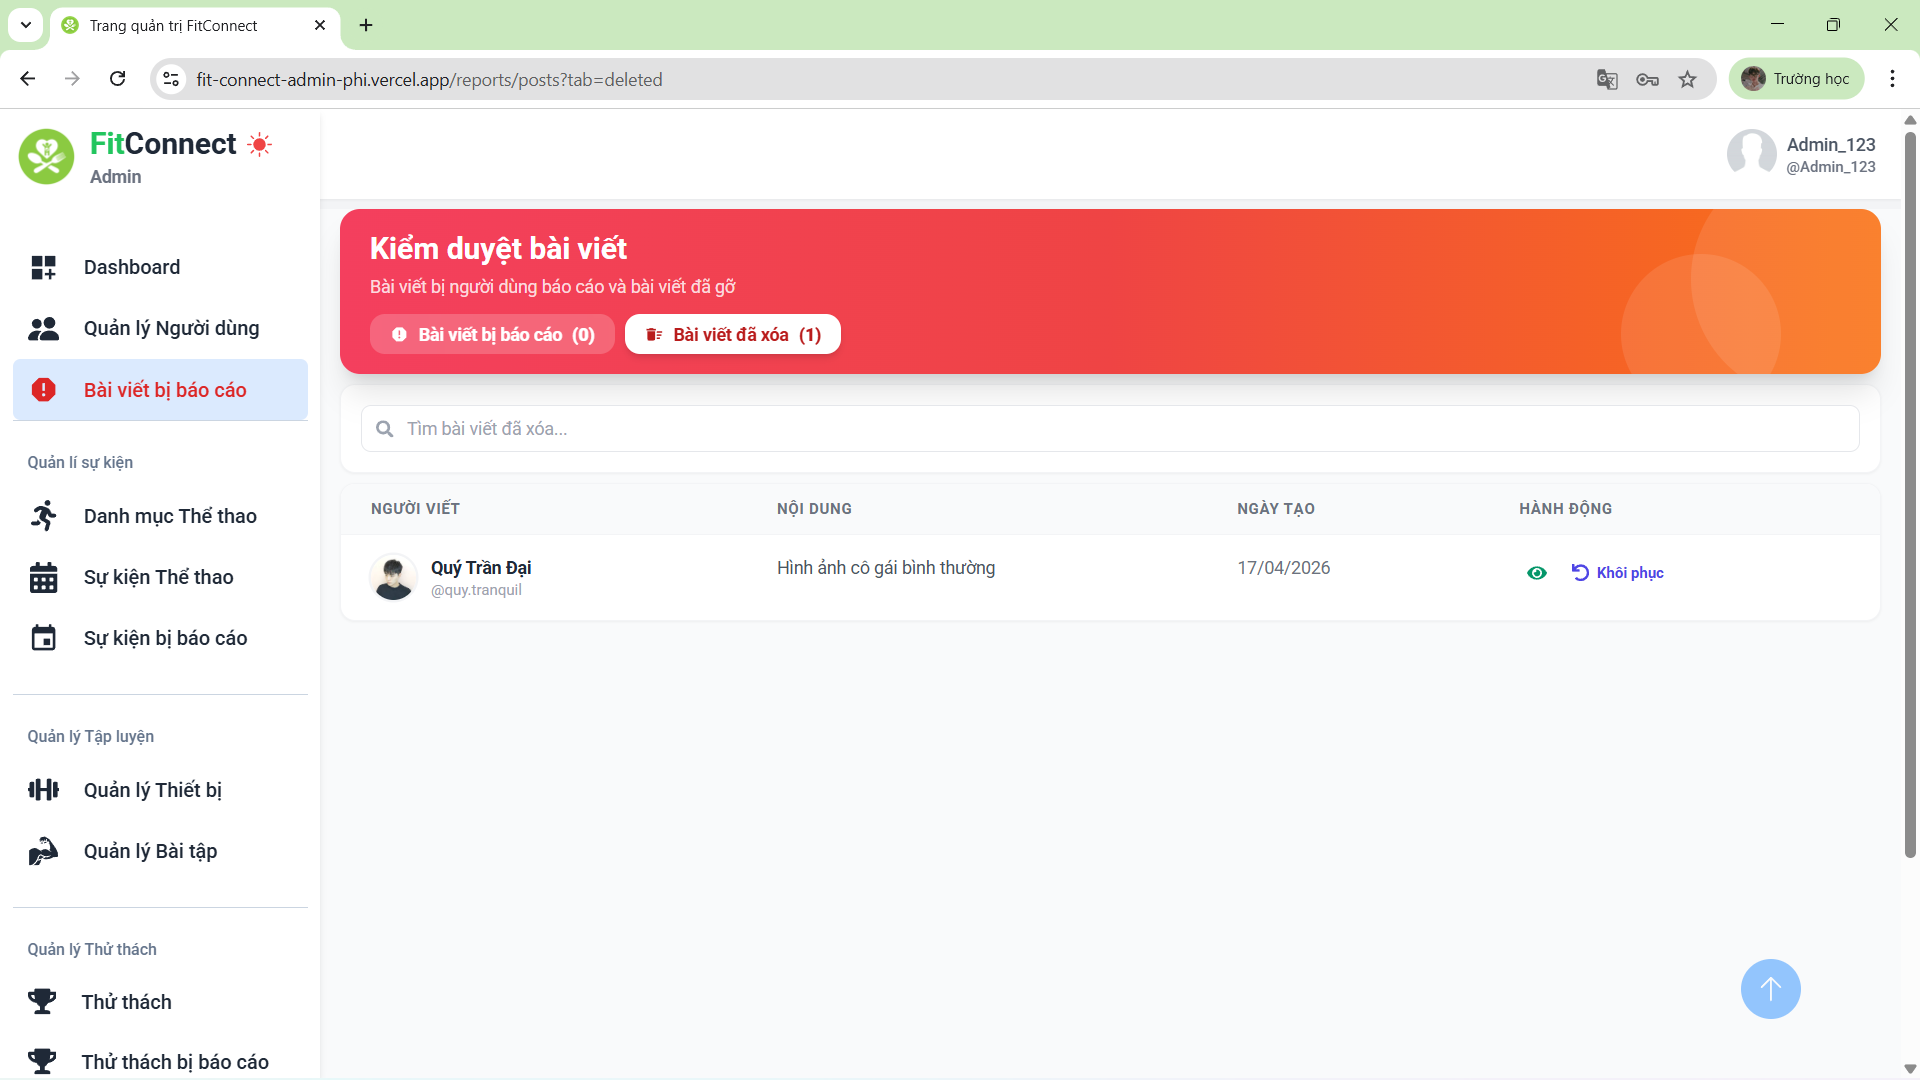
\includegraphics[width=\textwidth]{Images/IMG/Nhom2/hienthibenbaivietbixoa.png}
        \caption{Danh sách bài viết đã xóa và tùy chọn khôi phục}
        \label{fig:impl_social_admin_trash}
    \end{subfigure}
    \vspace{0.3em}
    \caption{Giao diện kiểm duyệt và quản lý bài viết vi phạm của Admin}
    \label{fig:impl_social_admin_moderation}
\end{figure}

\end{itemize}

\subsection{Nhóm tính năng Sự kiện thể thao}
\label{subsec:impl_sport_event}

Nhóm tính năng Sự kiện thể thao cho phép người dùng tổ chức và tham gia các sự kiện thể thao cộng đồng. Hệ thống hỗ trợ hai hình thức tổ chức: Ngoài trời (chạy bộ, đạp xe, leo núi,...) với tính năng theo dõi tiến độ bằng GPS, và Trong nhà (Gym, Yoga, Cardio,...) với tính năng tập luyện qua Video Call có AI theo dõi sự hiện diện. Ngoài ra, hệ thống còn tích hợp AI để hỗ trợ người dùng tạo sự kiện tự động chỉ bằng một đoạn mô tả ngắn.

Quy trình hoạt động gồm ba luồng chính:
\begin{itemize}
    \item \textbf{Người dùng (Người tổ chức):} Tạo, quản lý sự kiện, theo dõi danh sách người tham gia và chỉnh sửa thông tin sự kiện.
    \item \textbf{Người dùng (Người tham gia):} Tìm kiếm, tham gia sự kiện, ghi tiến độ hoạt động, chia sẻ và mời bạn bè.
    \item \textbf{Quản trị viên:} Xử lý các sự kiện bị báo cáo từ cộng đồng.
\end{itemize}

\subsubsection{Luồng thao tác tạo và quản lý sự kiện (Góc độ Người tổ chức)}
\begin{itemize}
    \item Người dùng truy cập trang Sự kiện thể thao, sẽ thấy danh sách các sự kiện thể thao phù hợp nhất kèm theo những sự kiện thể thao nổi bật nhất được hiển thị dạng banner lớn ở đầu trang. Người dùng có thể lọc theo hình thức (Ngoài trời, Trong nhà) và theo danh mục môn thể thao (Cardio, Chạy bộ, Yoga,...).

\begin{figure}[H]
    \centering
    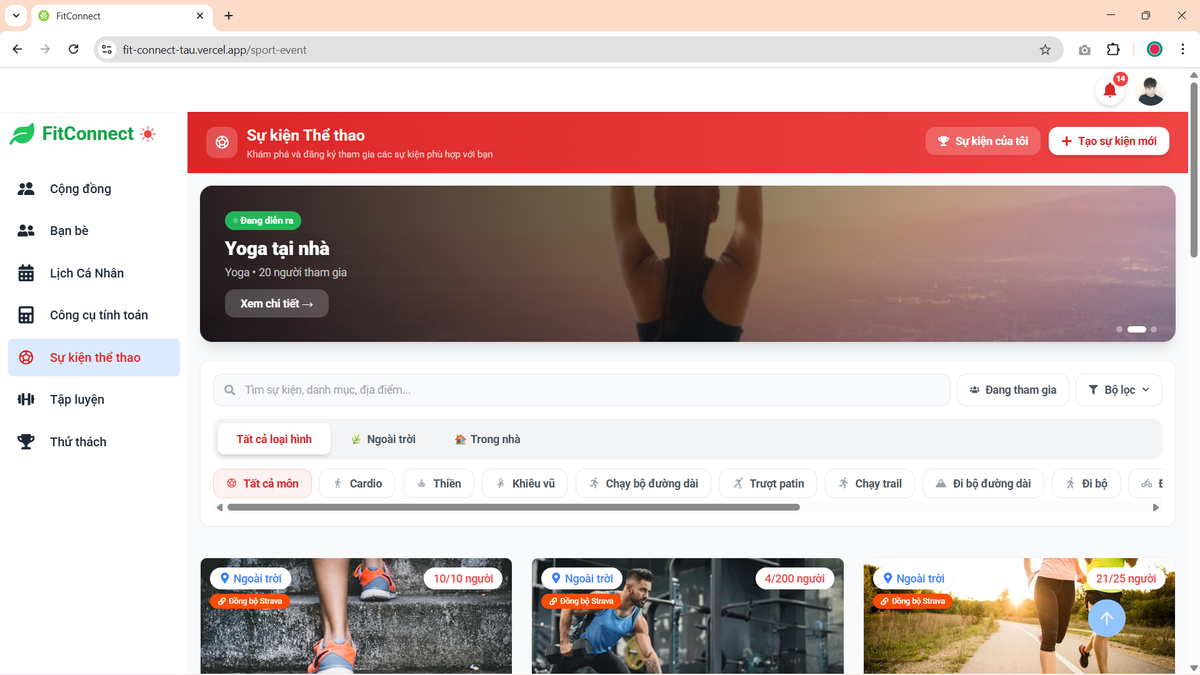
\includegraphics[width=0.60\textwidth]{Images/IMG/nhom3/danhsachsukien.png}
    \caption{Người dùng xem danh sách sự kiện thể thao}
    \label{fig:impl_se_list}
\end{figure}


    \item Người dùng nhấn Tạo sự kiện mới, hệ thống hiển thị trang tạo sự kiện thể thao bao gồm các thông tin: (1) Thông tin chung -- tên sự kiện, danh mục thể thao, hình thức tổ chức (Ngoài trời hoặc Trong nhà); (2) Thời gian \& Địa điểm -- ngày bắt đầu, ngày kết thúc, thời điểm, địa điểm cụ thể; (3) Mục tiêu \& Sức chứa -- số người tối đa, mục tiêu sự kiện (km hoặc kcal); (4) Hình ảnh \& Mô tả -- ảnh bìa, mô tả ngắn, mô tả chi tiết, yêu cầu tham gia, lợi ích khi tham gia.

\begin{figure}[H]
    \centering
    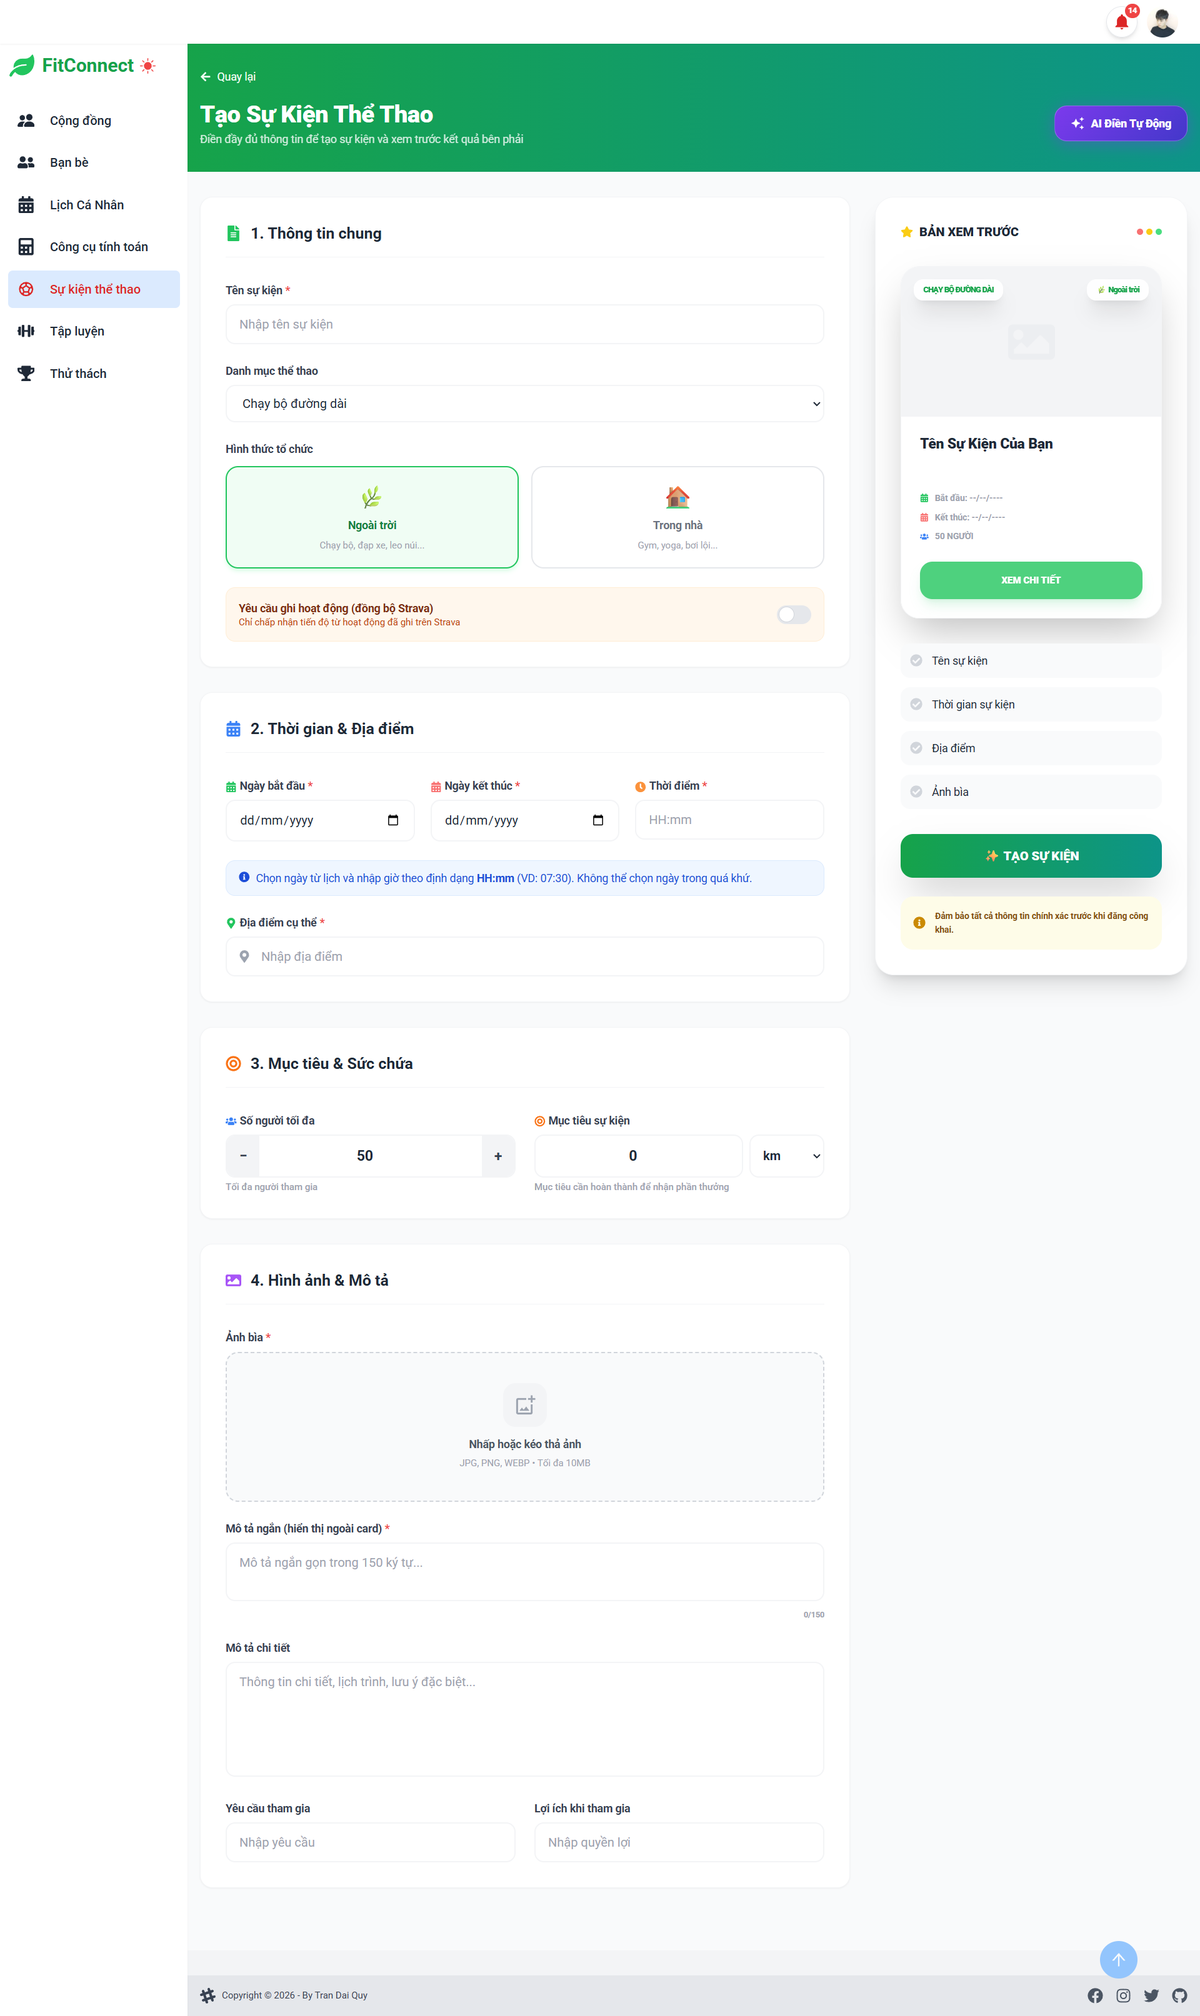
\includegraphics[width=0.60\textwidth]{Images/IMG/nhom3/taosukien.png}
    \caption{Người dùng thao tác tạo sự kiện thể thao mới}
    \label{fig:impl_se_create}
\end{figure}


    \item Người dùng có thể dùng tính năng AI Điền Tự Động để tự động tạo sự kiện thể thao theo yêu cầu. Người dùng chỉ cần mô tả sơ bộ về sự kiện (ví dụ: ``Tạo sự kiện chạy bộ ngoài trời, ở công viên Hoàng Văn Thụ từ 18h hôm nay tới tháng sau''), AI sẽ tự động điền toàn bộ biểu mẫu tạo sự kiện bao gồm tên sự kiện, danh mục, thời gian, địa điểm, mục tiêu và mô tả chi tiết.

\begin{figure}[H]
    \centering
    \begin{subfigure}[b]{0.47\textwidth}
        \centering
        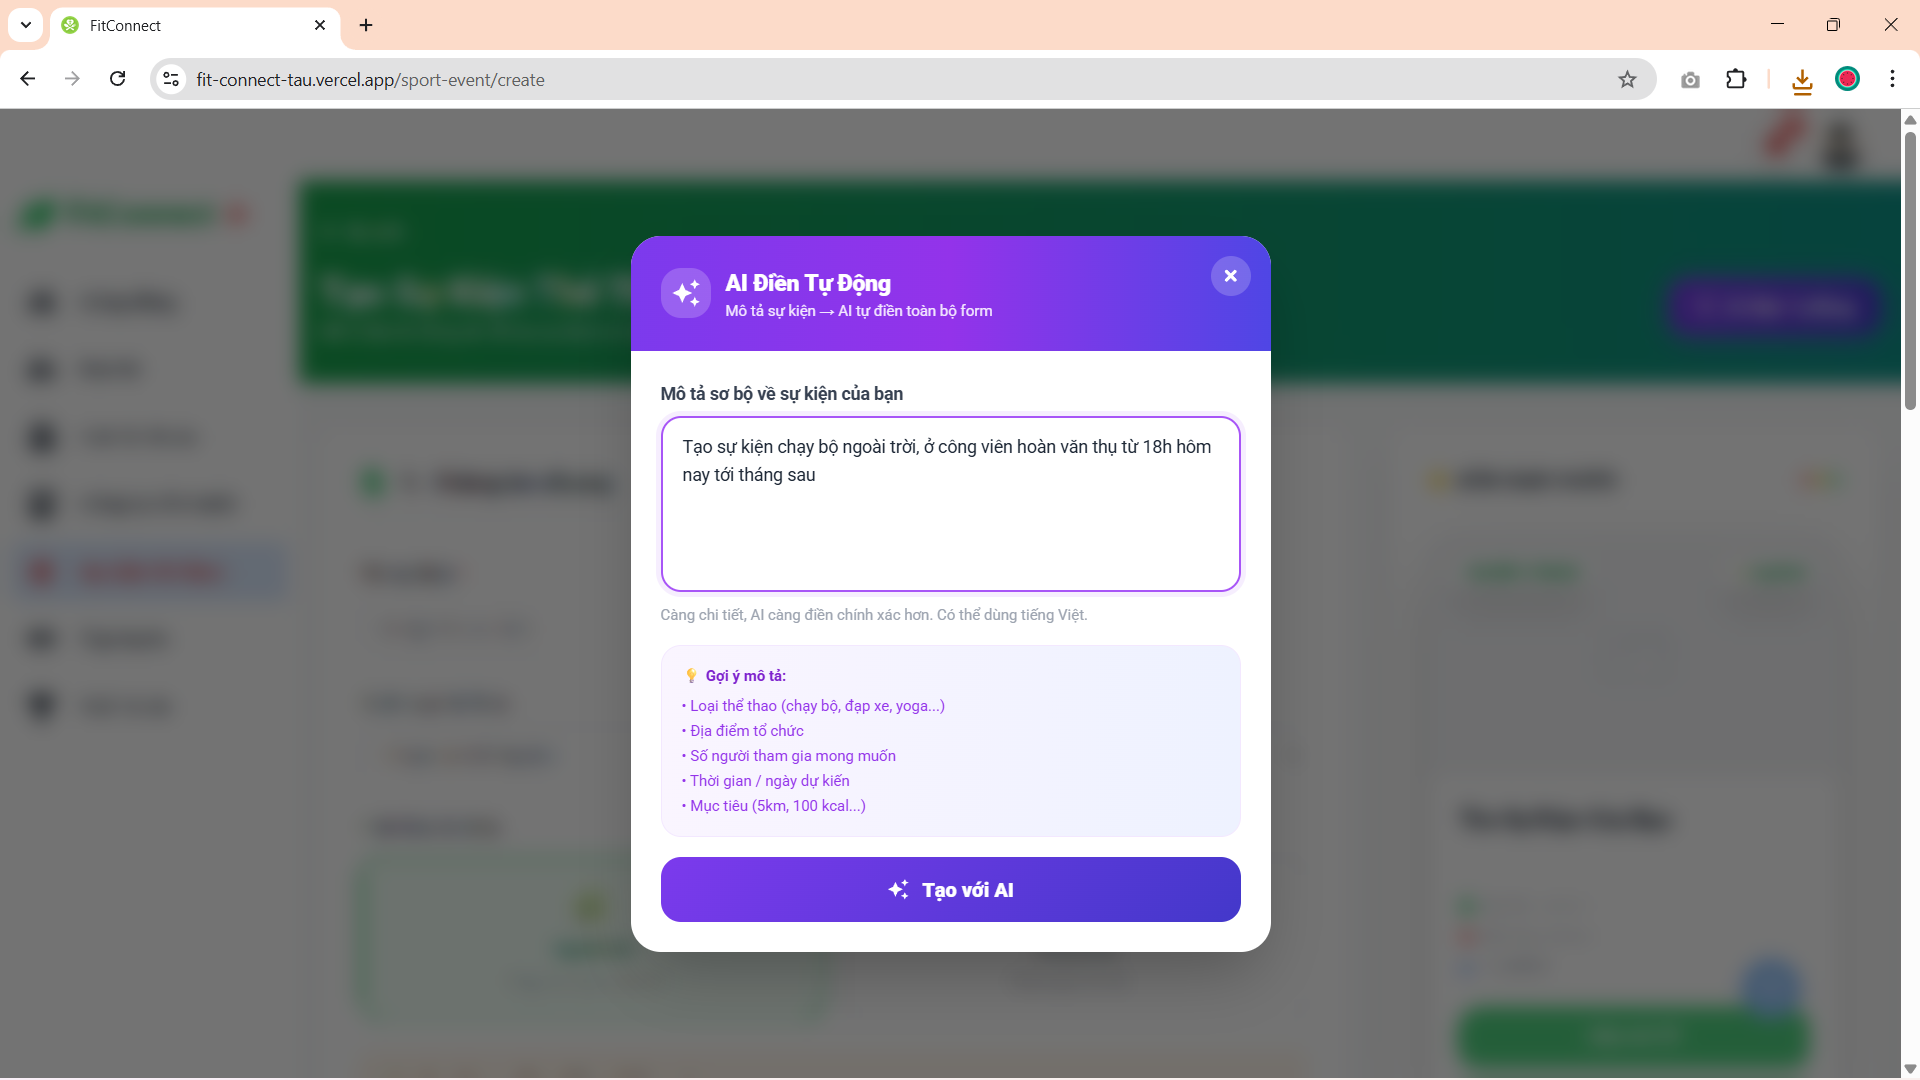
\includegraphics[width=\textwidth]{Images/IMG/nhom3/modaldienAItaosukientudong.png}
        \caption{Hệ thống hiển thị modal AI Điền Tự Động tạo sự kiện}
        \label{fig:impl_se_ai_modal}
    \end{subfigure}
    \hfill
    \begin{subfigure}[b]{0.47\textwidth}
        \centering
        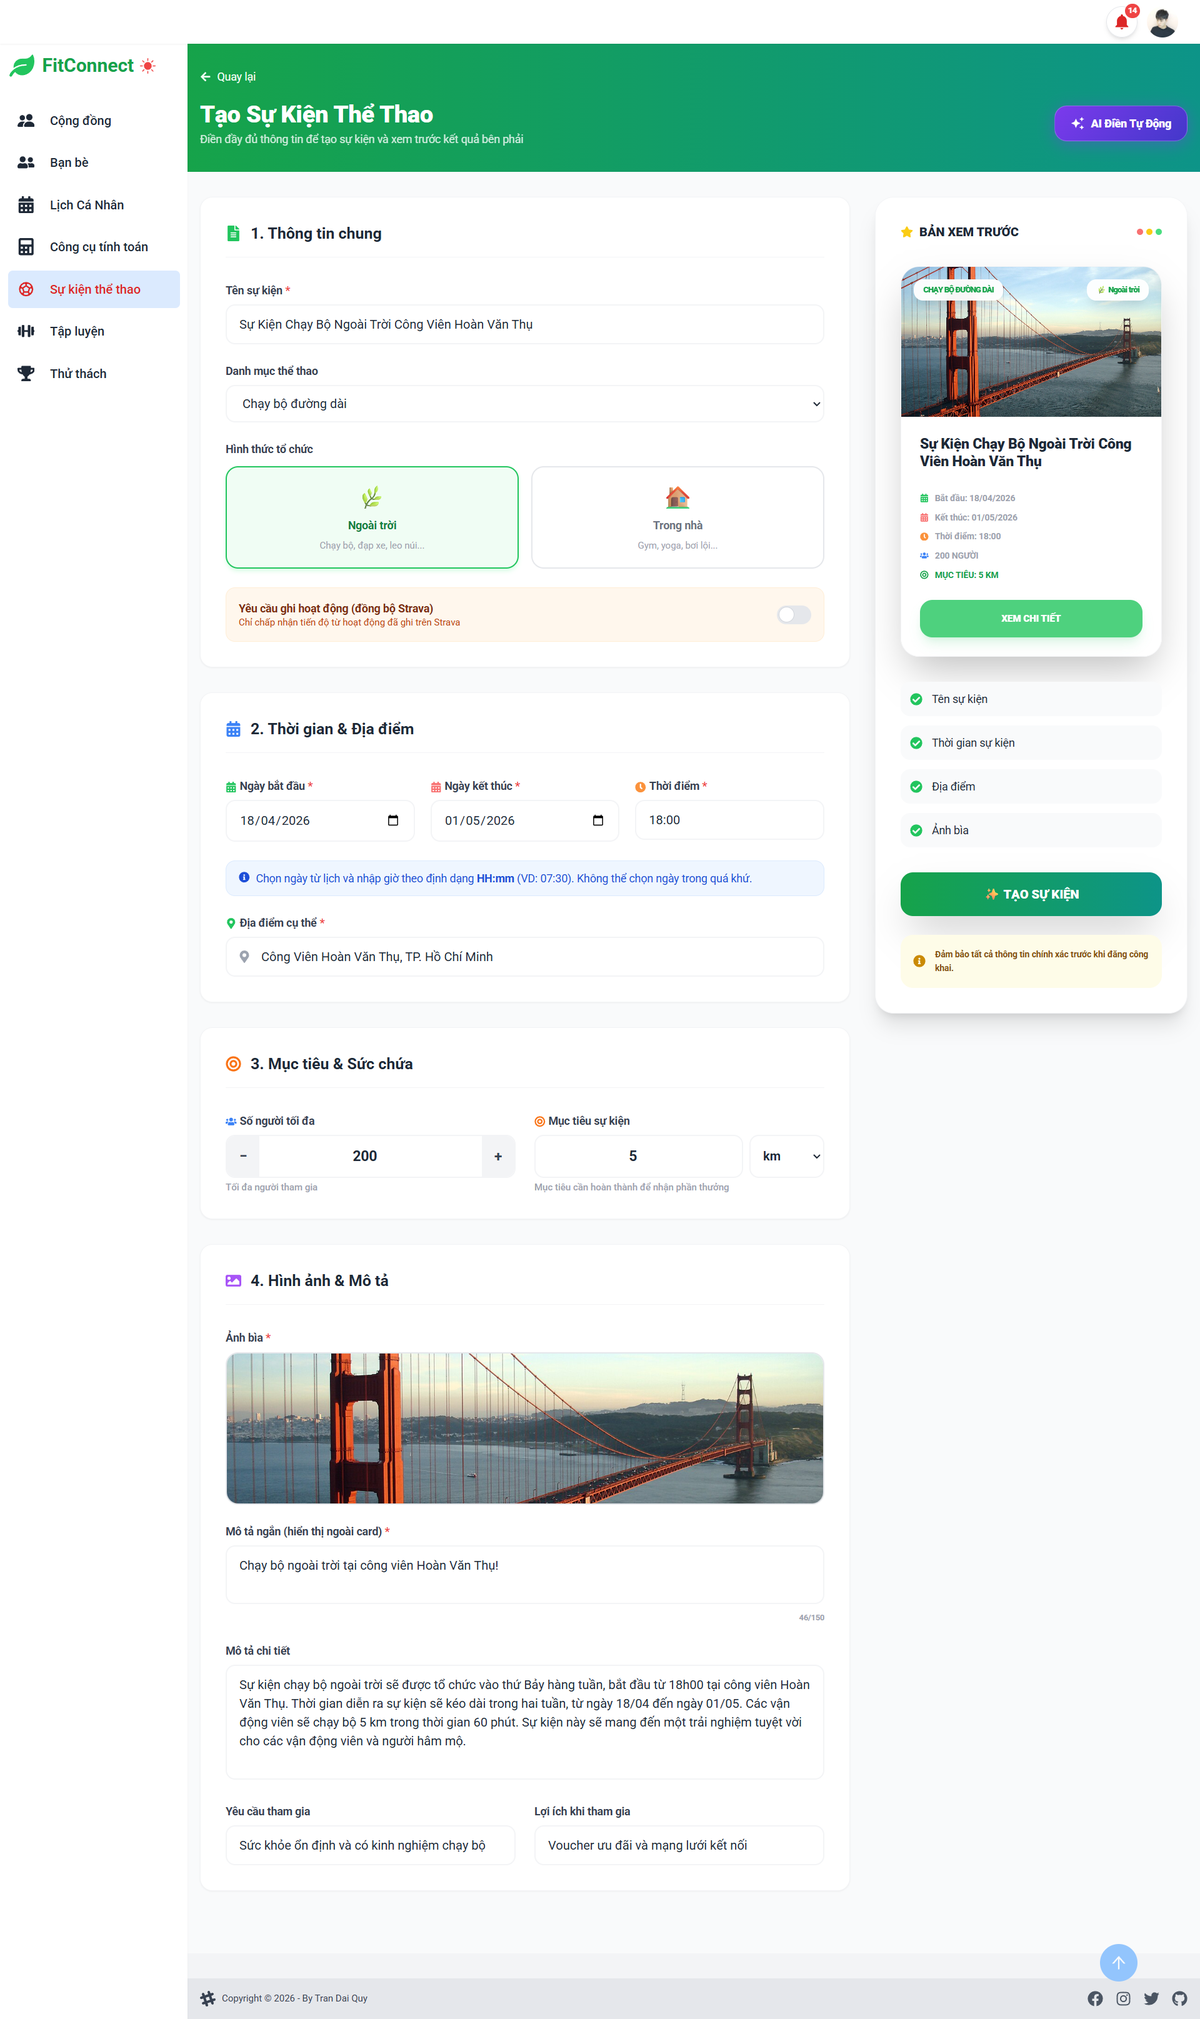
\includegraphics[width=\textwidth]{Images/IMG/nhom3/taobangAIthanhcong.png}
        \caption{Hệ thống tự động điền thông tin sự kiện sau khi AI xử lý thành công}
        \label{fig:impl_se_ai_success}
    \end{subfigure}
\end{figure}


    \item Sau khi nhấn Tạo sự kiện, hệ thống tự động điều hướng đến trang chi tiết sự kiện vừa tạo (người tạo đã được đăng ký tham gia mặc định). Tại trang ``Sự kiện của tôi'', người dùng quản lý được toàn bộ sự kiện đã tạo và đã tham gia.

\begin{figure}[H]
    \centering
    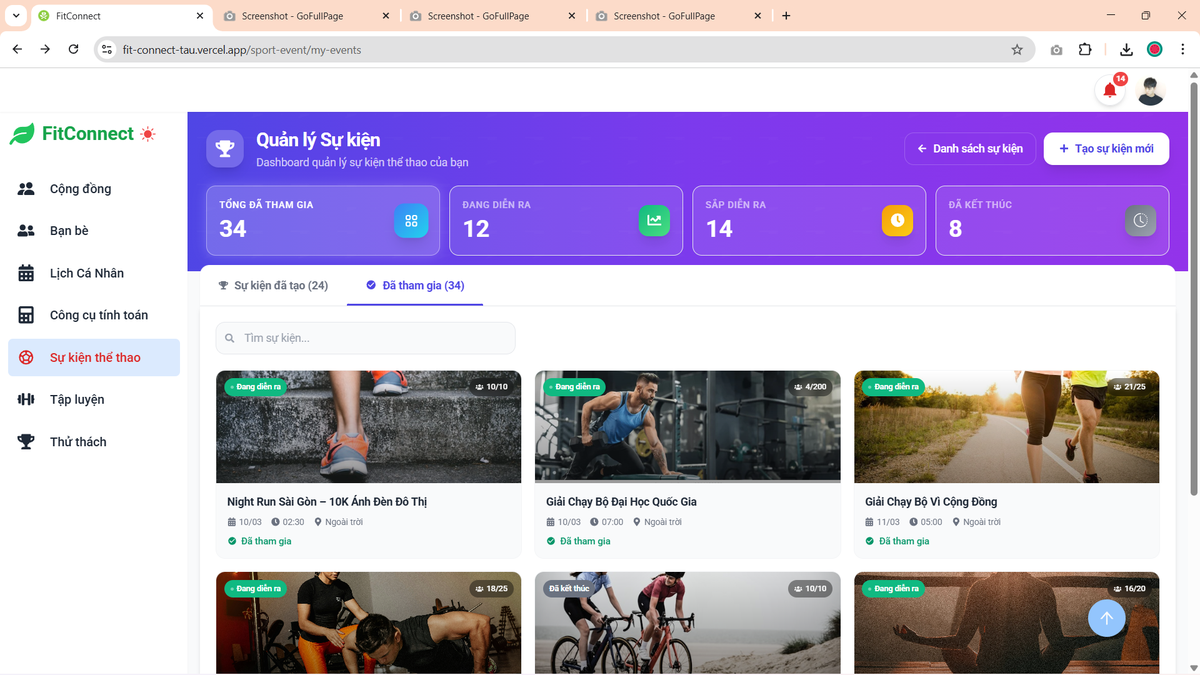
\includegraphics[width=0.60\textwidth]{Images/IMG/nhom3/quanlysukien.png}
    \caption{Người dùng xem trang quản lý sự kiện của tôi}
    \label{fig:impl_se_my_events}
\end{figure}


    \begin{itemize}
        \item Với những sự kiện đã tạo, người tổ chức có thể xem tổng quan sự kiện, xem danh sách những người tham gia (theo dõi tiến độ, xóa/sửa danh sách), và xem cài đặt sự kiện.

\begin{figure}[H]
    \centering
    \begin{subfigure}[b]{0.30\textwidth}
        \centering
        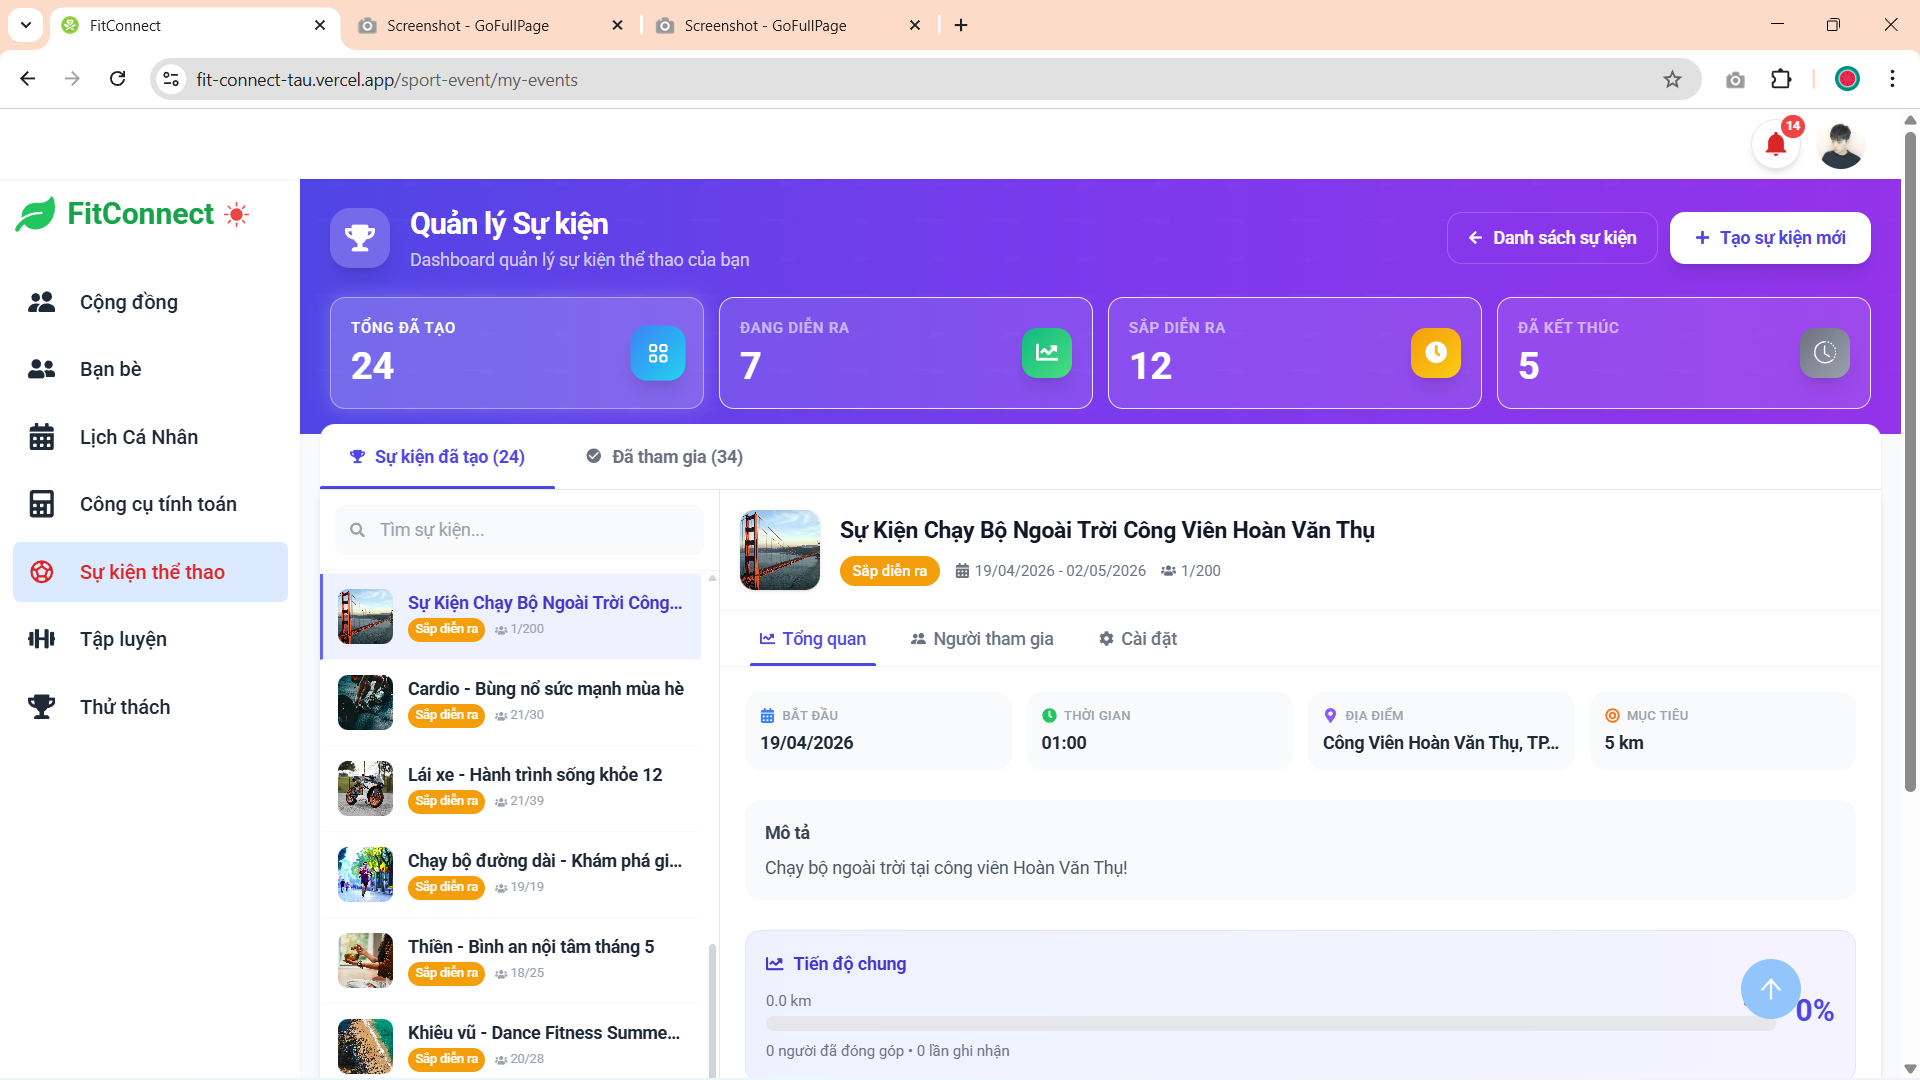
\includegraphics[width=\textwidth]{Images/IMG/nhom3/trangquanlysukienvatongquansk.png}
        \caption{Người tổ chức xem trang quản lý sự kiện và tổng quan sự kiện}
        \label{fig:impl_se_overview}
    \end{subfigure}
    \hfill
    \begin{subfigure}[b]{0.30\textwidth}
        \centering
        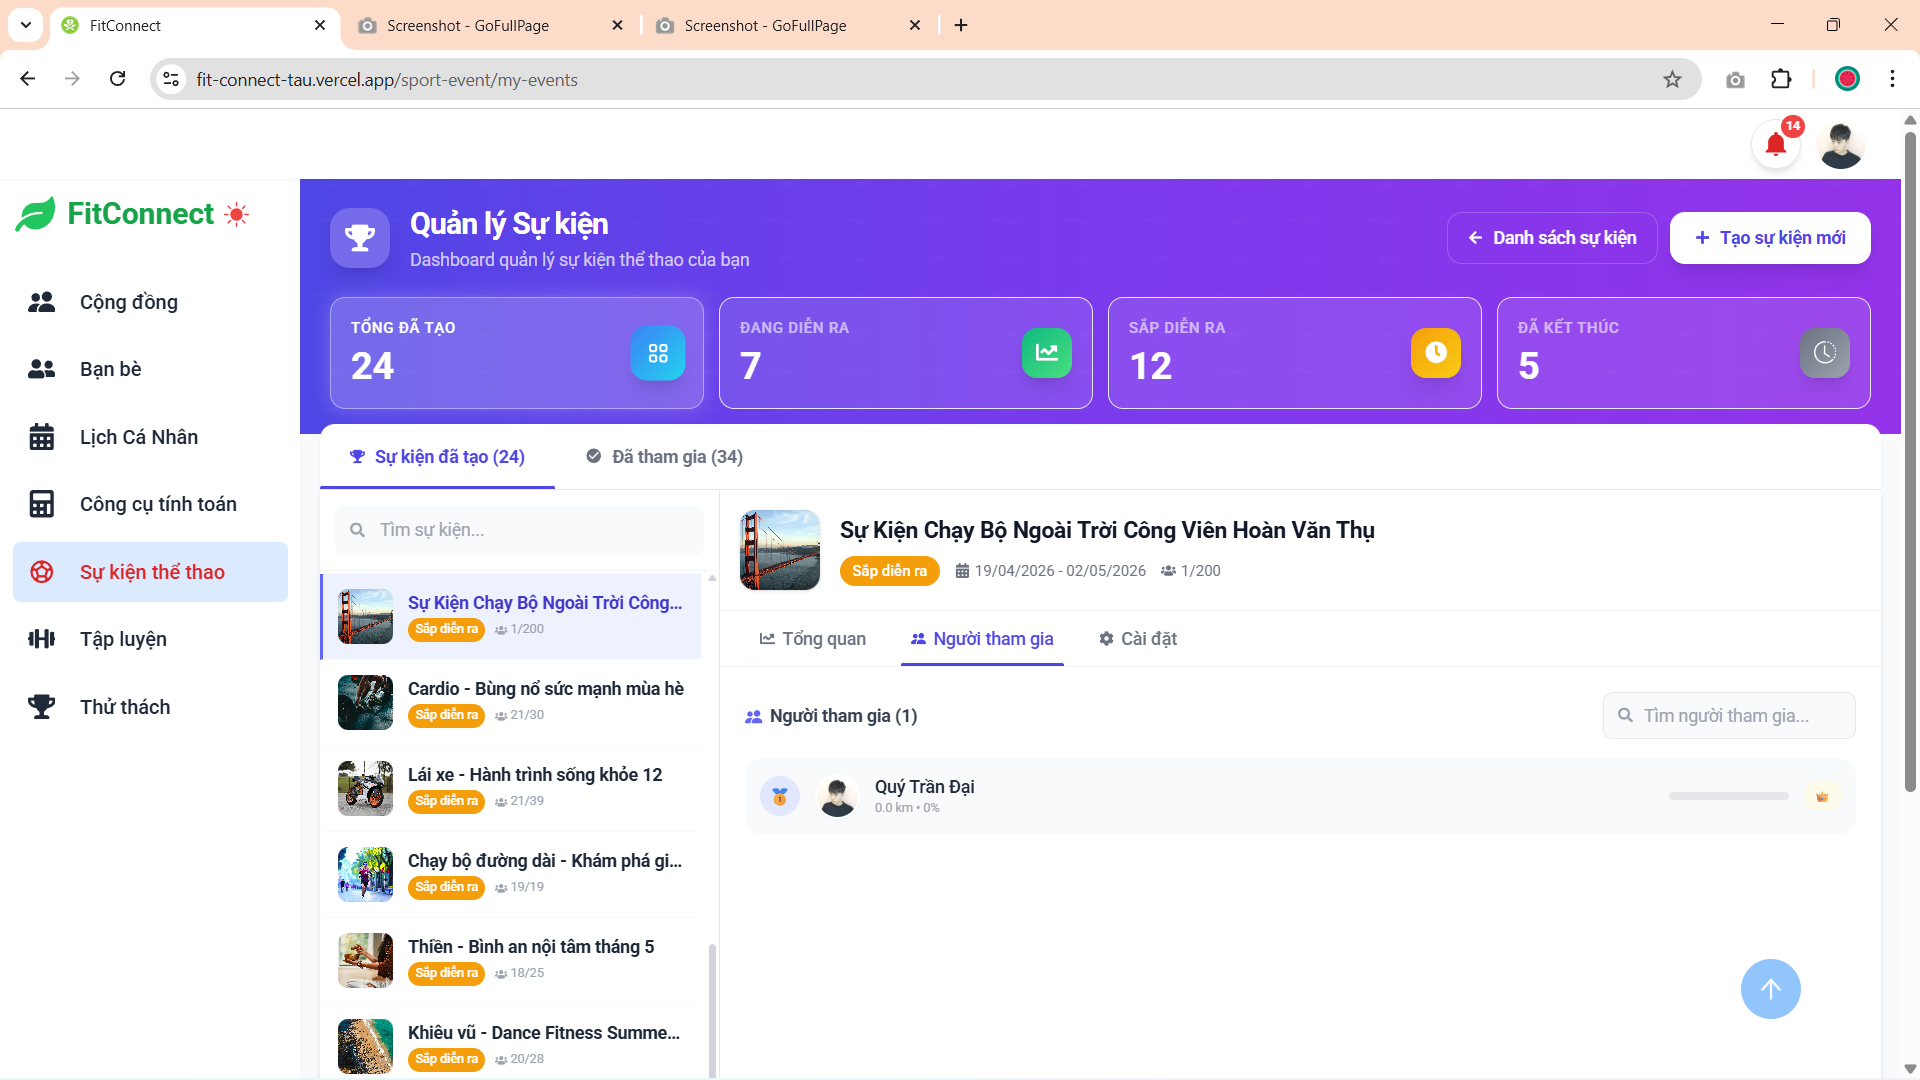
\includegraphics[width=\textwidth]{Images/IMG/nhom3/nguoithamgiasukientoidatao.png}
        \caption{Người tổ chức xem danh sách người tham gia sự kiện đã tạo}
        \label{fig:impl_se_participants}
    \end{subfigure}
    \hfill
    \begin{subfigure}[b]{0.30\textwidth}
        \centering
        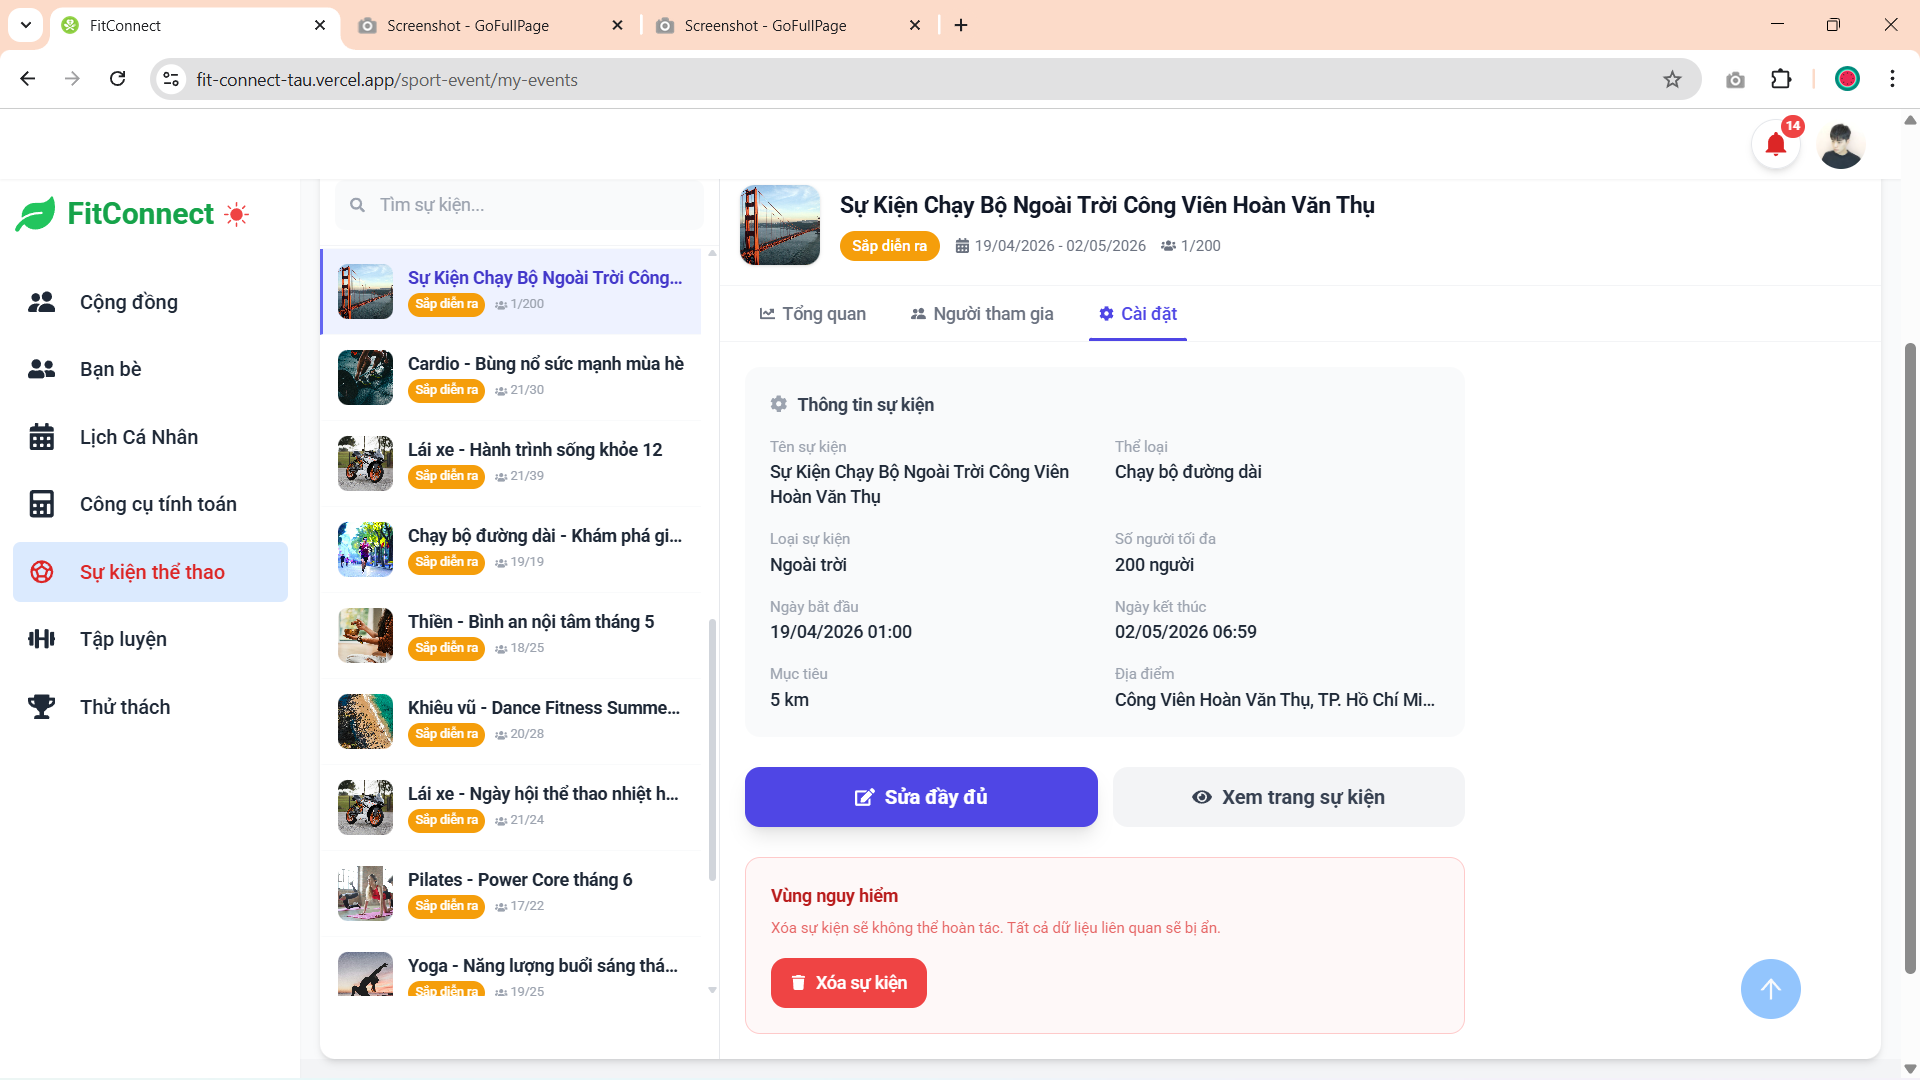
\includegraphics[width=\textwidth]{Images/IMG/nhom3/caidatsukientoidatao.png}
        \caption{Người tổ chức xem cài đặt sự kiện đã tạo}
        \label{fig:impl_se_settings}
    \end{subfigure}
\end{figure}


        \item Với chỉnh sửa sự kiện: Người tổ chức có thể chỉnh sửa thông tin sự kiện và nhấn Lưu để cập nhật, dữ liệu sự kiện sẽ được cập nhật theo những chỉnh sửa mới nhất.

\begin{figure}[H]
    \centering
    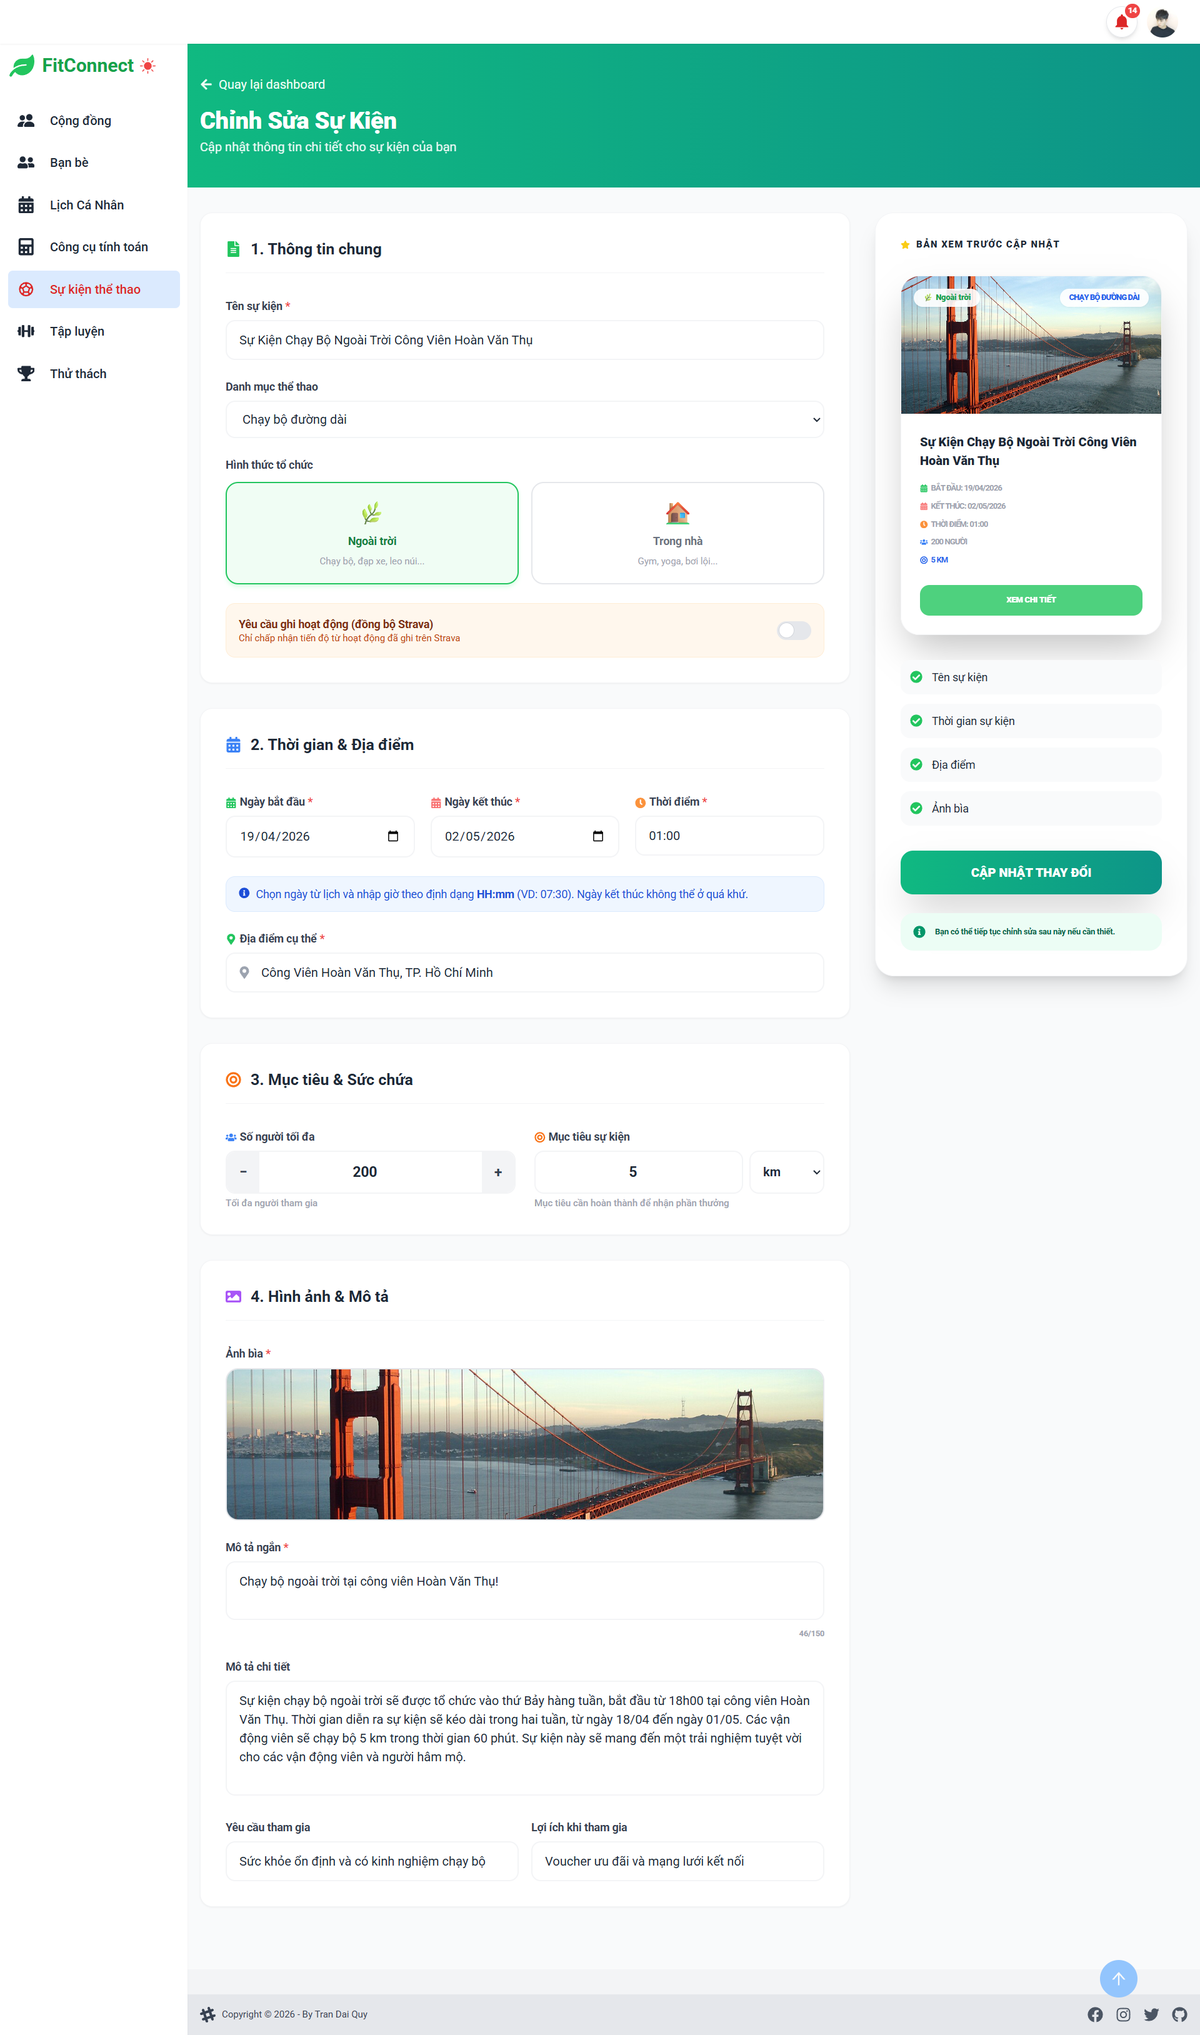
\includegraphics[width=0.60\textwidth]{Images/IMG/nhom3/chinhsuasukiencuatoi.png}
    \caption{Người tổ chức thao tác chỉnh sửa sự kiện của tôi}
    \label{fig:impl_se_edit}
\end{figure}


        \item Với xóa sự kiện: Người tổ chức có thể xóa sự kiện khi sự kiện chưa bắt đầu; hệ thống thực hiện xóa mềm (đánh dấu đã xóa), sự kiện không còn hiển thị phía người dùng nhưng vẫn được lưu trong dữ liệu hệ thống để Admin có thể khôi phục.

    \end{itemize}
\end{itemize}

\subsubsection{Luồng thao tác tham gia sự kiện (Góc độ Người tham gia)}
\begin{itemize}
    \item Với người dùng không phải là người tổ chức, ở trang danh sách sự kiện có thể lọc và tìm kiếm sự kiện để tham gia. Khi nhấn tham gia sự kiện, hệ thống sẽ chuyển đến trang chi tiết sự kiện hiển thị toàn bộ thông tin bao gồm: mô tả sự kiện, thời gian, địa điểm, mục tiêu, tiến độ tổng quan của nhóm, thống kê sự kiện, bảng xếp hạng và danh sách người tham gia.

\begin{figure}[H]
    \centering
    \begin{subfigure}[b]{0.47\textwidth}
        \centering
        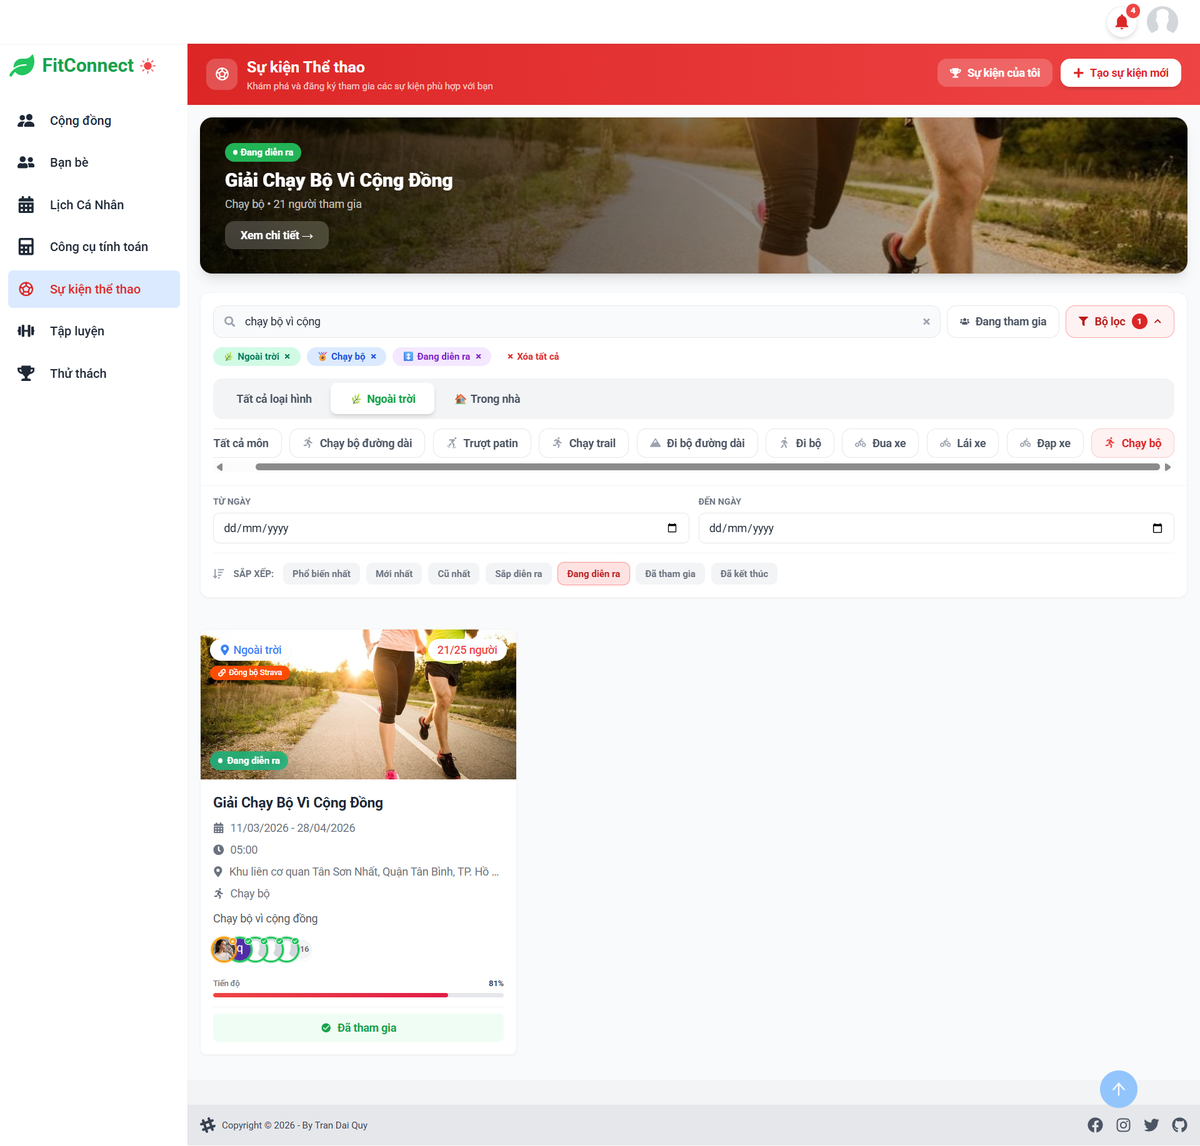
\includegraphics[width=\textwidth]{Images/IMG/nhom3/timkiemsukienvathamgiasukien.png}
        \caption{Người dùng thao tác tìm kiếm và tham gia sự kiện}
        \label{fig:impl_se_search_join}
    \end{subfigure}
    \hfill
    \begin{subfigure}[b]{0.47\textwidth}
        \centering
        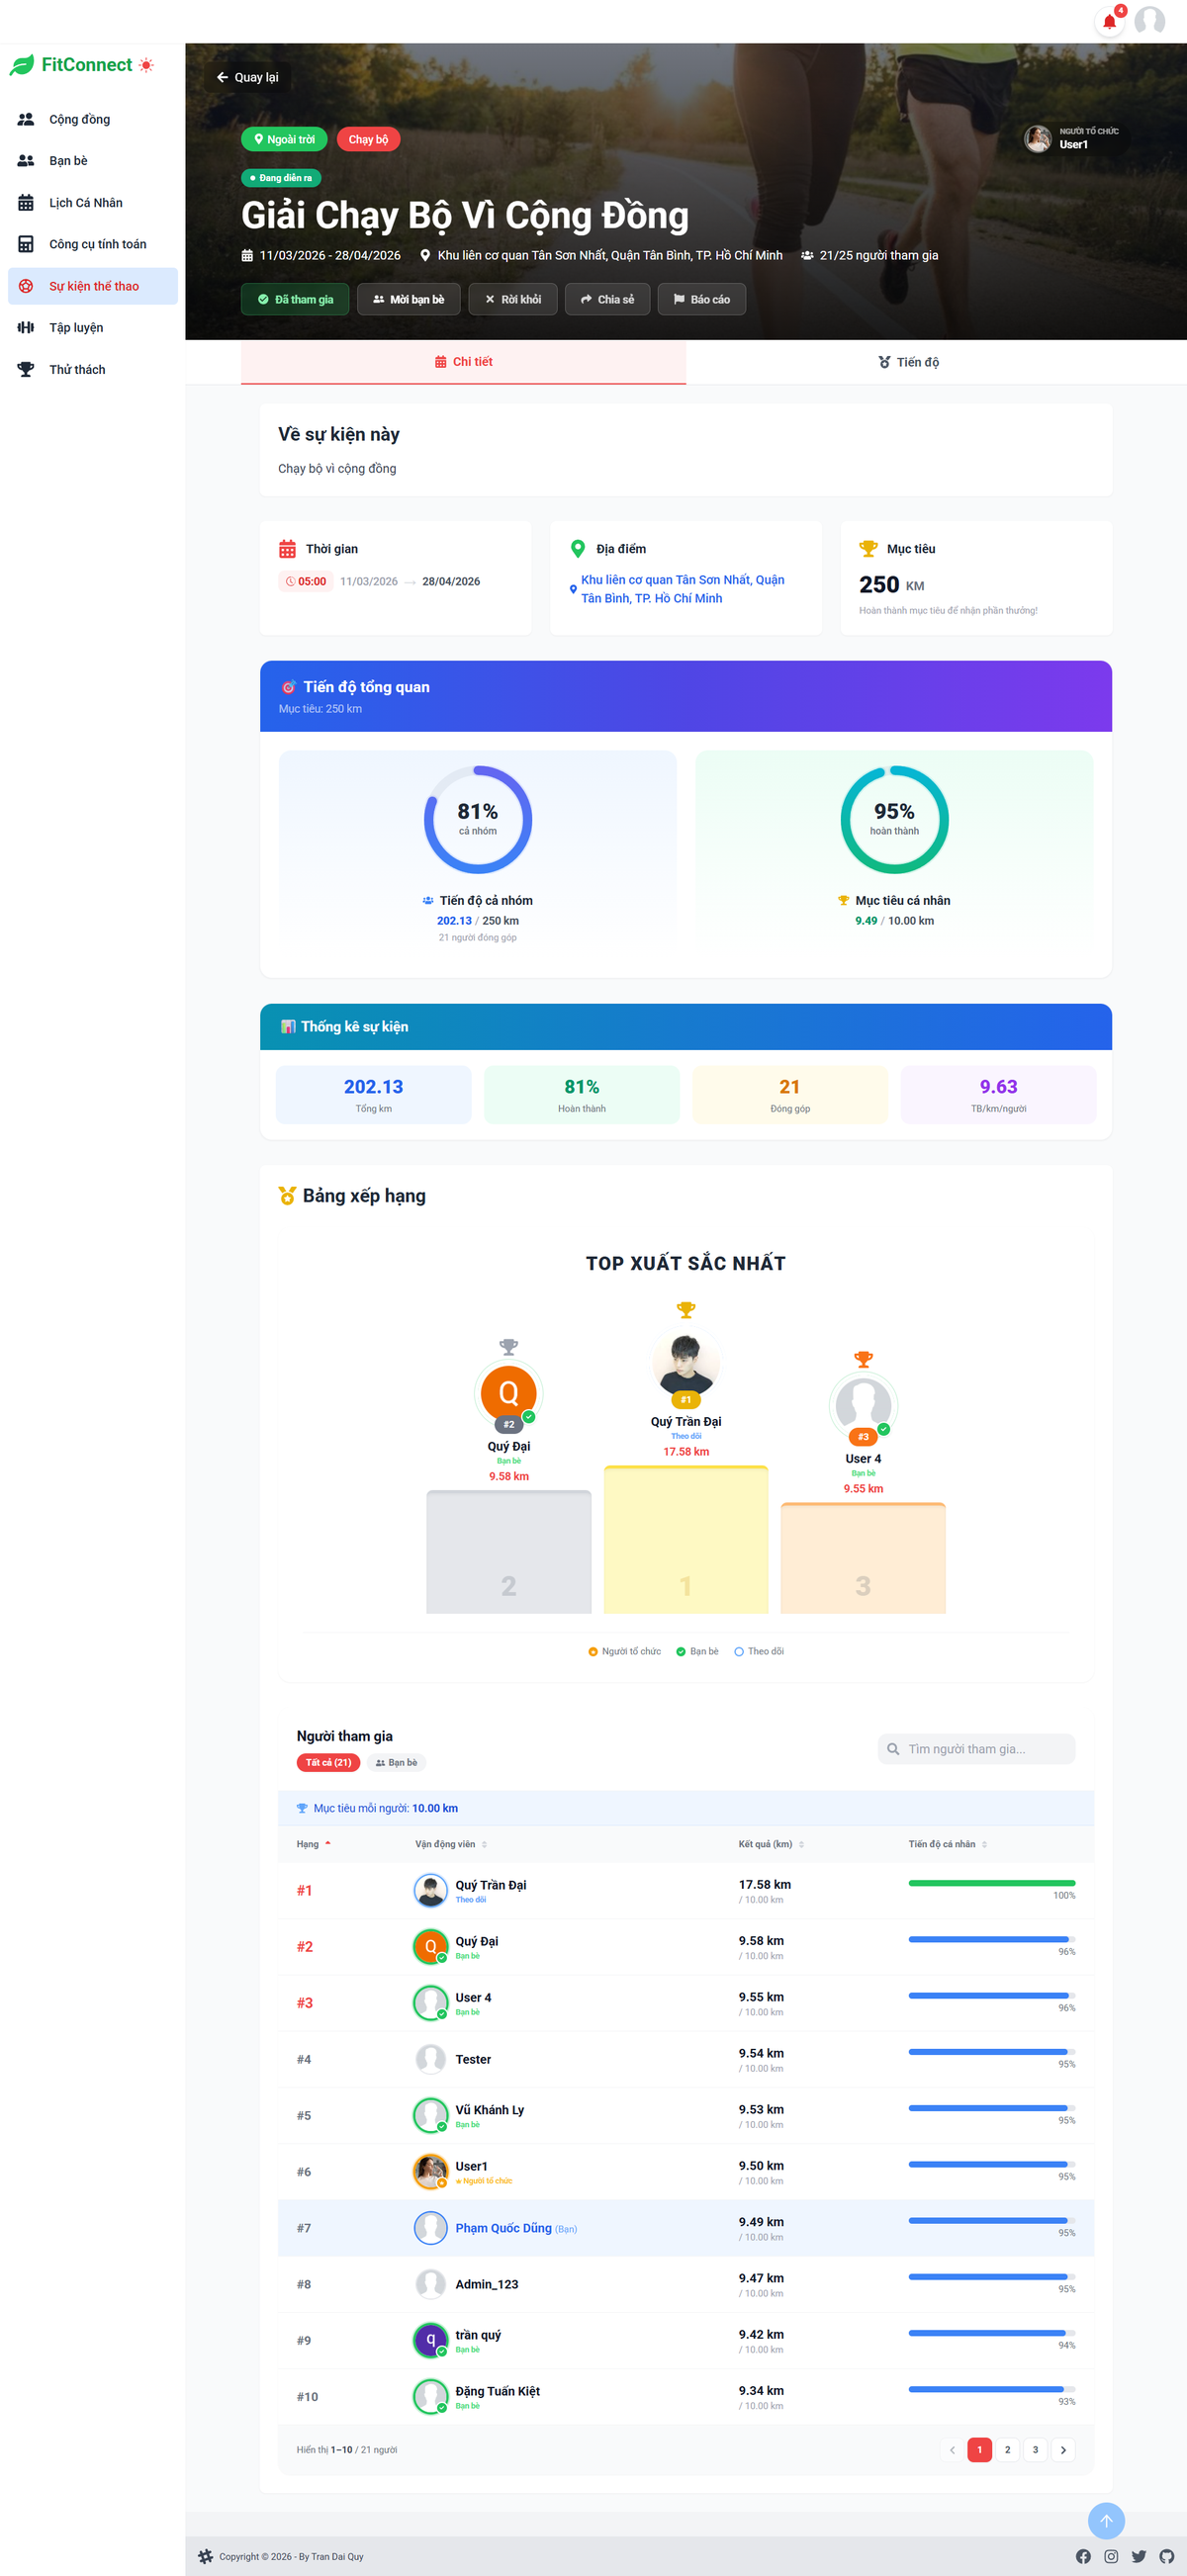
\includegraphics[width=\textwidth]{Images/IMG/nhom3/thongtinchitietsukien.png}
        \caption{Hệ thống hiển thị thông tin chi tiết sự kiện thể thao}
        \label{fig:impl_se_detail}
    \end{subfigure}
\end{figure}


    \item Người tham gia có thể chia sẻ sự kiện lên trang Cộng đồng để lan tỏa và mời thêm người tham gia; bài viết sự kiện sẽ tự động xuất hiện trên Bảng tin.

\begin{figure}[H]
    \centering
    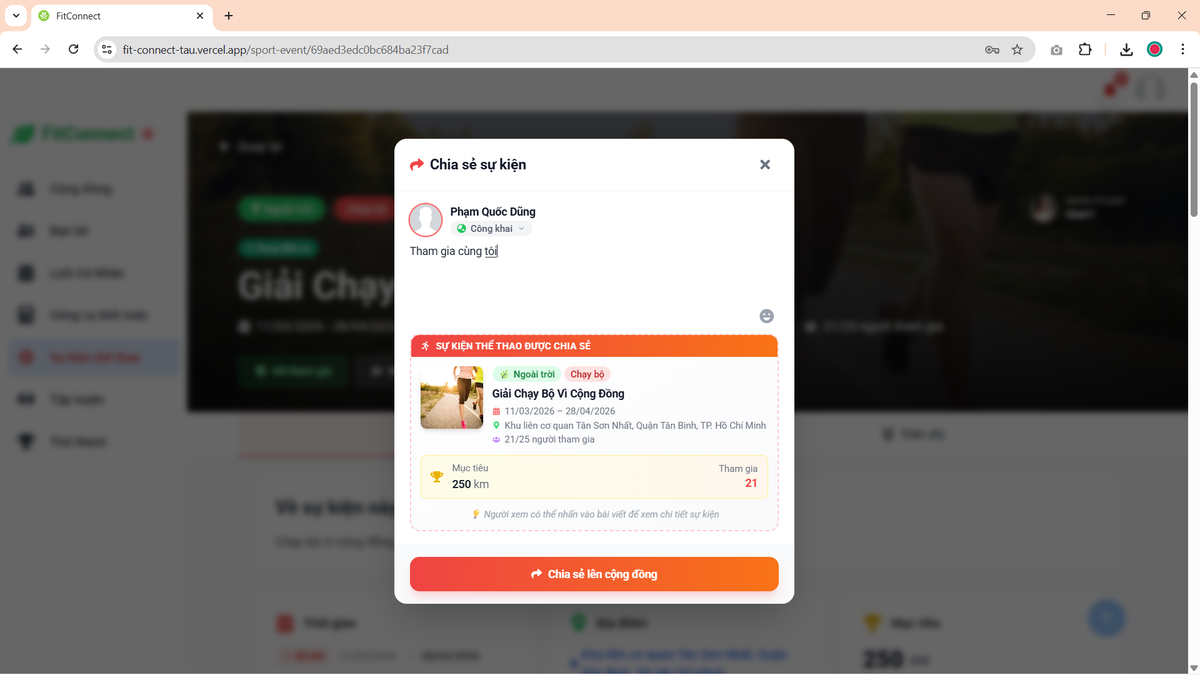
\includegraphics[width=0.60\textwidth]{Images/IMG/nhom3/chiasesukienngoaitroi.png}
    \caption{Người tham gia thao tác chia sẻ sự kiện ngoài trời lên cộng đồng}
    \label{fig:impl_se_share}
\end{figure}


    \item Người tham gia có thể mời bạn bè tham gia sự kiện. Người được mời sẽ nhận thông báo được mời tham gia sự kiện, nhấn vào thông báo sẽ chuyển đến trang sự kiện được mời.

\begin{figure}[H]
    \centering
    \begin{subfigure}[b]{0.47\textwidth}
        \centering
        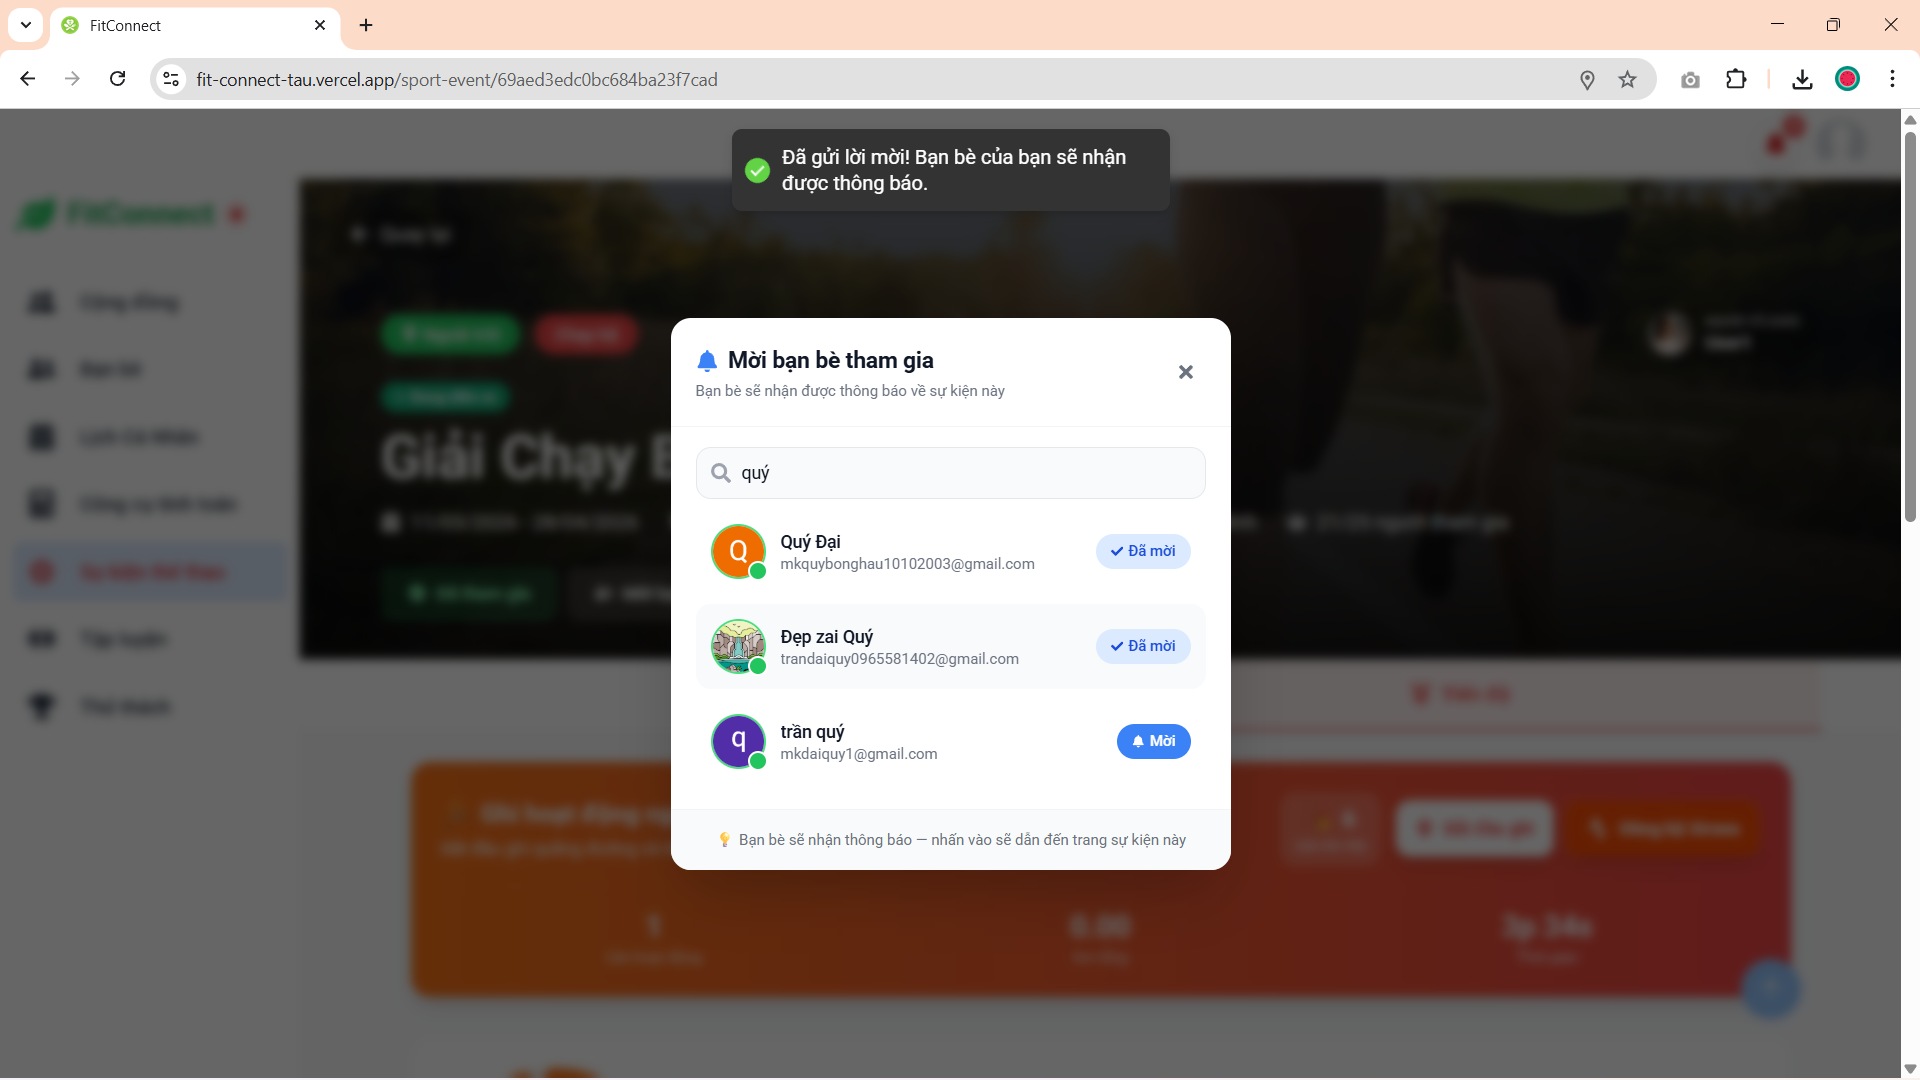
\includegraphics[width=\textwidth]{Images/IMG/nhom3/modalmoimoinguoithamgia.png}
        \caption{Người tham gia thao tác mời mọi người tham gia sự kiện}
        \label{fig:impl_se_invite}
    \end{subfigure}
    \hfill
    \begin{subfigure}[b]{0.47\textwidth}
        \centering
        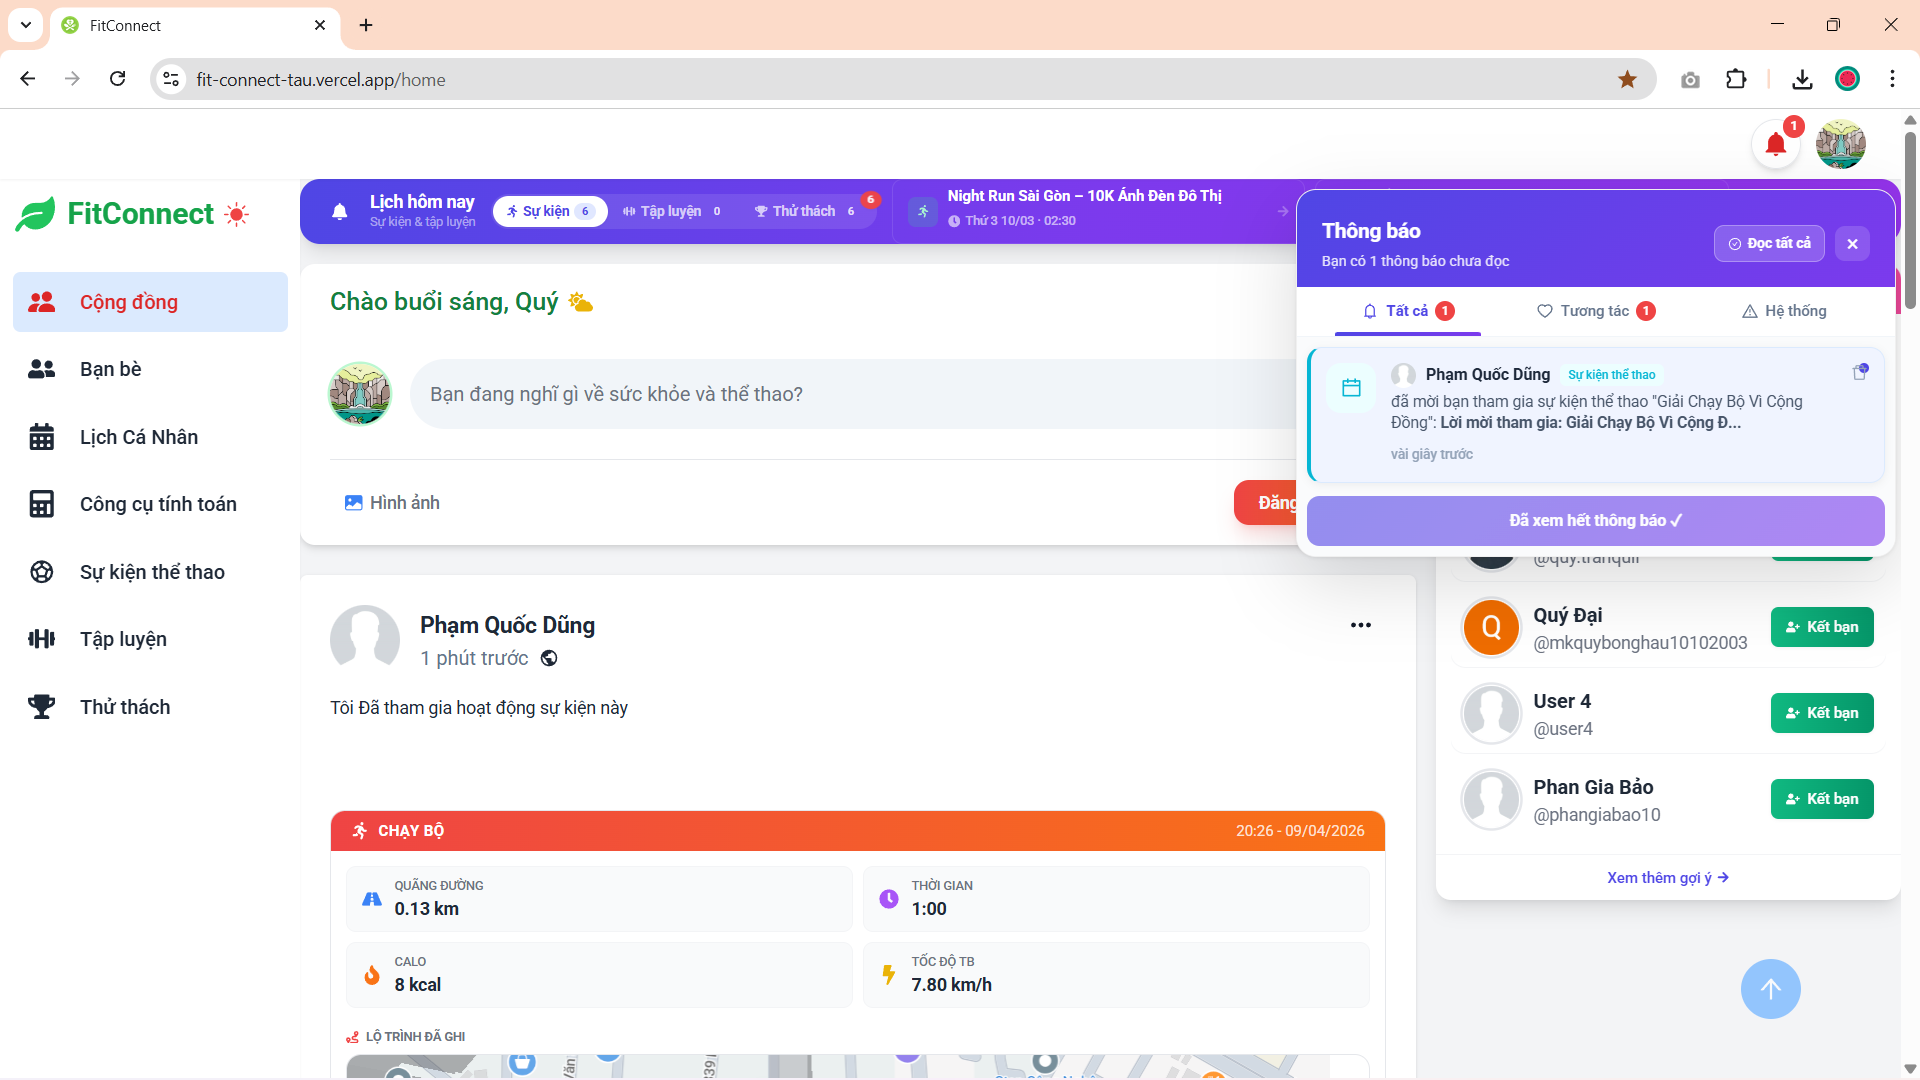
\includegraphics[width=\textwidth]{Images/IMG/nhom3/nguoidcmoithaythongbaomoisk.png}
        \caption{Người được mời nhận thông báo mời tham gia sự kiện}
        \label{fig:impl_se_invite_noti}
    \end{subfigure}
\end{figure}


    \item Người tham gia có thể báo cáo sự kiện vi phạm lên Quản trị viên.

\begin{figure}[H]
    \centering
    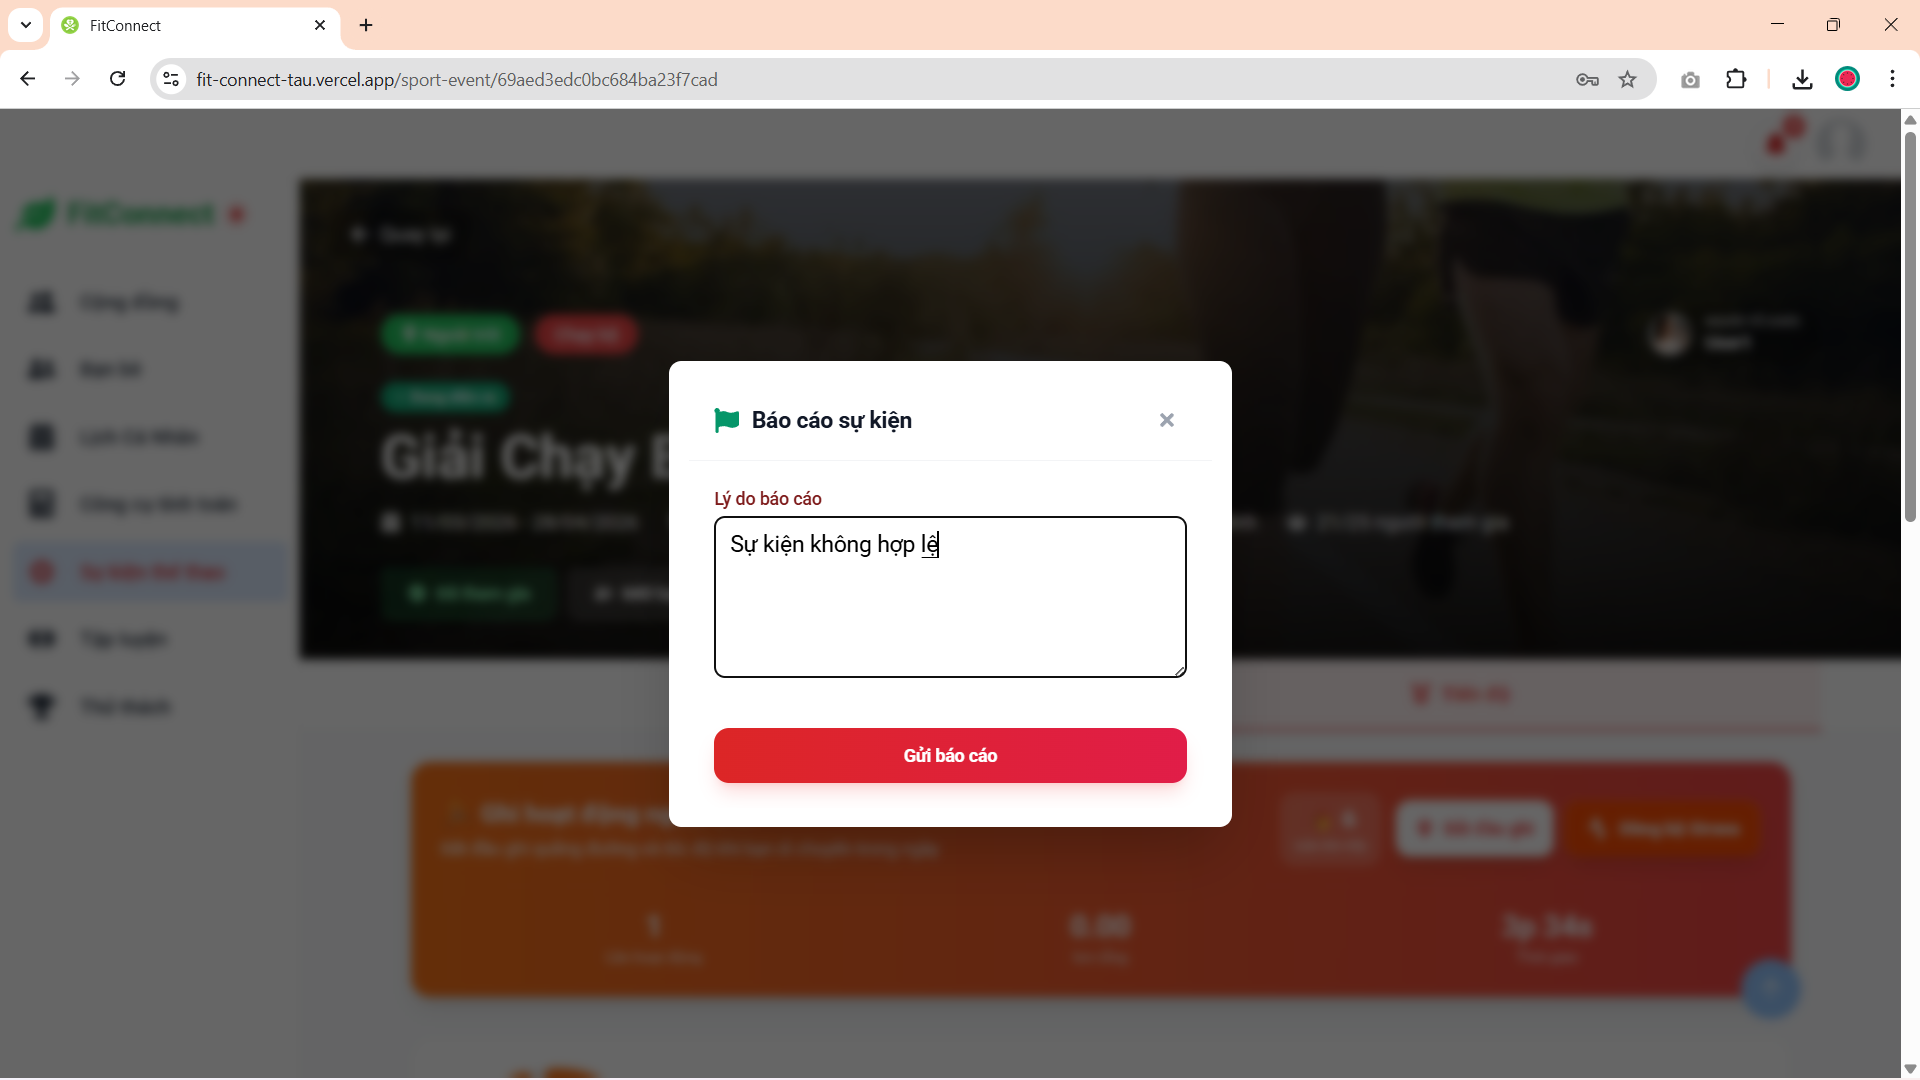
\includegraphics[width=0.60\textwidth]{Images/IMG/nhom3/baocaosukien.png}
    \caption{Người tham gia thao tác báo cáo sự kiện}
    \label{fig:impl_se_report}
\end{figure}

\end{itemize}

\textbf{Tiến độ sự kiện Ngoài trời:}
\begin{itemize}
    \item Đối với sự kiện Ngoài trời, người tham gia có thể nhấn vào tab Tiến độ và xem được thông tin tiến độ tổng quan bao gồm: phần trăm hoàn thành mục tiêu cá nhân, tiến độ đạt được (km), thống kê chi tiết (quãng đường, calories, lần hoạt động, vận tốc trung bình), biểu đồ lịch sử hoạt động và danh sách các hoạt động gần đây.

\begin{figure}[H]
    \centering
    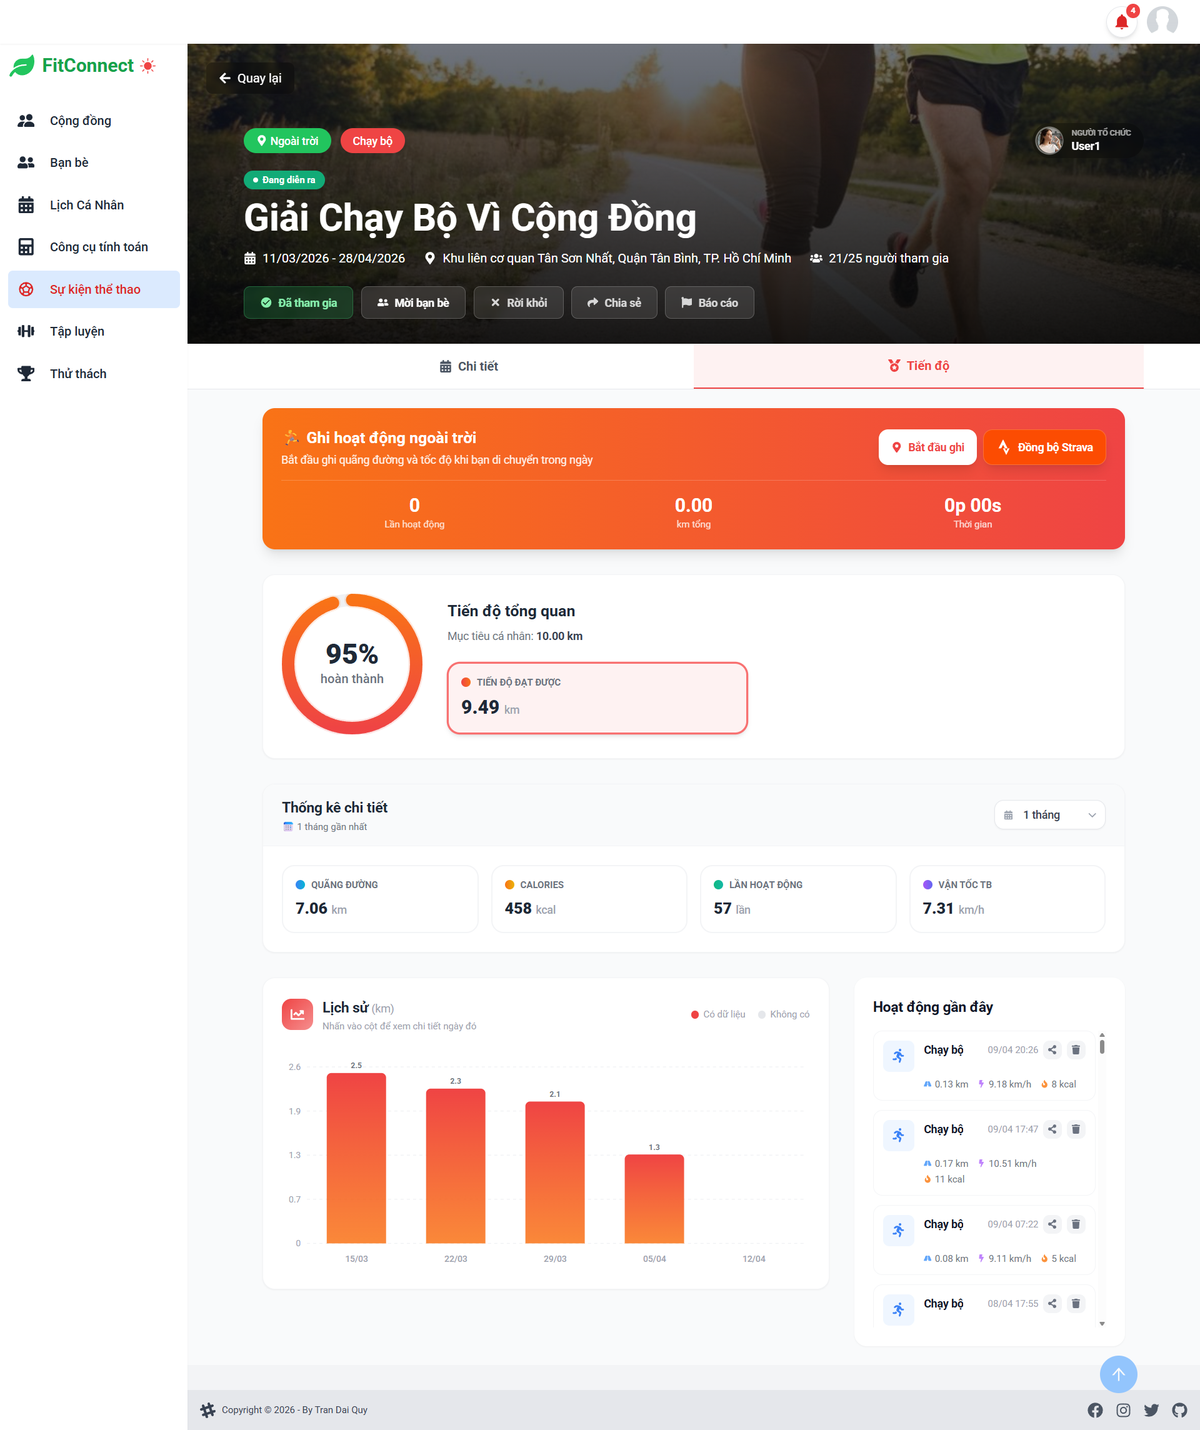
\includegraphics[width=0.60\textwidth]{Images/IMG/nhom3/trangtiendosukien.png}
    \caption{Người tham gia xem trang tiến độ sự kiện ngoài trời}
    \label{fig:impl_se_progress_outdoor}
\end{figure}


    \item Người tham gia có thể ghi tiến độ dựa trên GPS Tracking.
    \begin{itemize}
        \item Khi người tham gia nhấn Bắt đầu ghi (GPS Tracking), hệ thống sẽ hiển thị trang bản đồ với vị trí hiện tại, quãng đường đã đi (km), thời gian, tốc độ (km/h), calories đã đốt (kcal) và thanh tiến độ mục tiêu.

\begin{figure}[H]
    \centering
    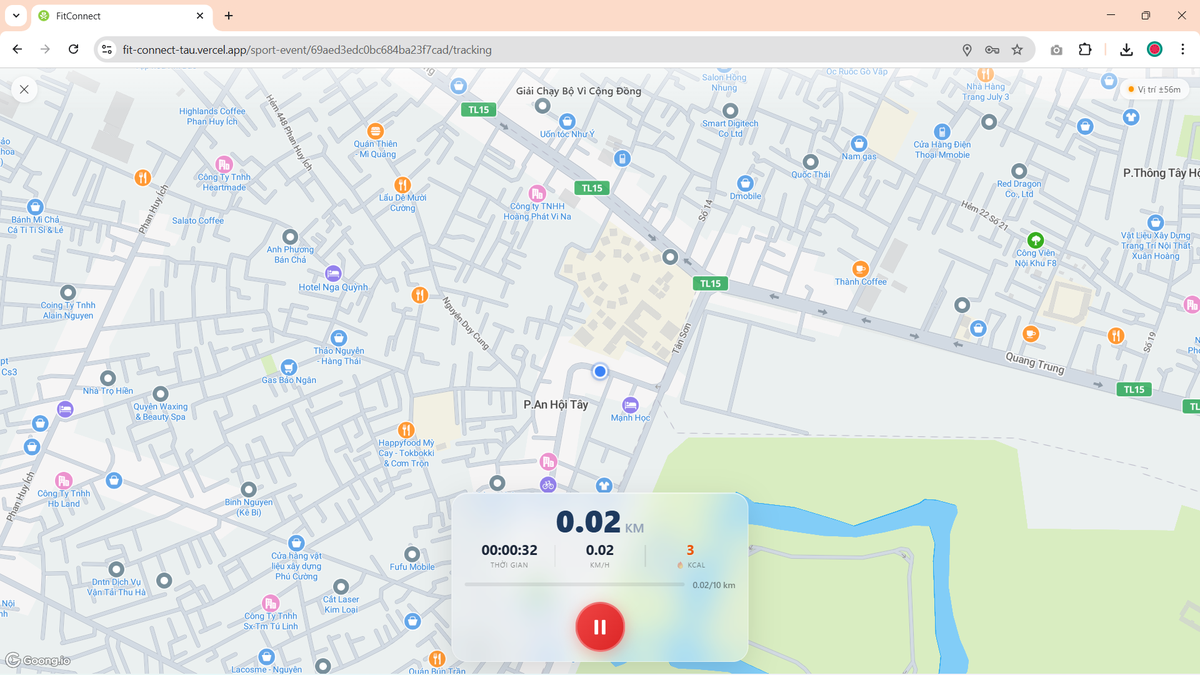
\includegraphics[width=0.60\textwidth]{Images/IMG/nhom3/trackinggpssukienngoaitroi.png}
    \caption{Người tham gia ghi tiến độ bằng GPS tracking sự kiện ngoài trời}
    \label{fig:impl_se_gps}
\end{figure}


        \item Người tham gia nhấn hoàn thành, hệ thống tổng hợp và hiển thị kết quả hoạt động vừa ghi: quãng đường (km), thời gian hoạt động và calories (kcal), đồng thời tự động cập nhật tiến độ sự kiện.


        \item Sau khi hoạt động được lưu, người tham gia có thể nhấn vào từng bản ghi trong danh sách ``Hoạt động gần đây'' để xem chi tiết. Hệ thống hiển thị modal chi tiết hoạt động ngoài trời gồm: loại hoạt động, thời điểm ghi nhận, quãng đường, thời gian, calories, vận tốc trung bình/tối đa và bản đồ lộ trình GPS đã ghi.

\begin{figure}[H]
    \centering
    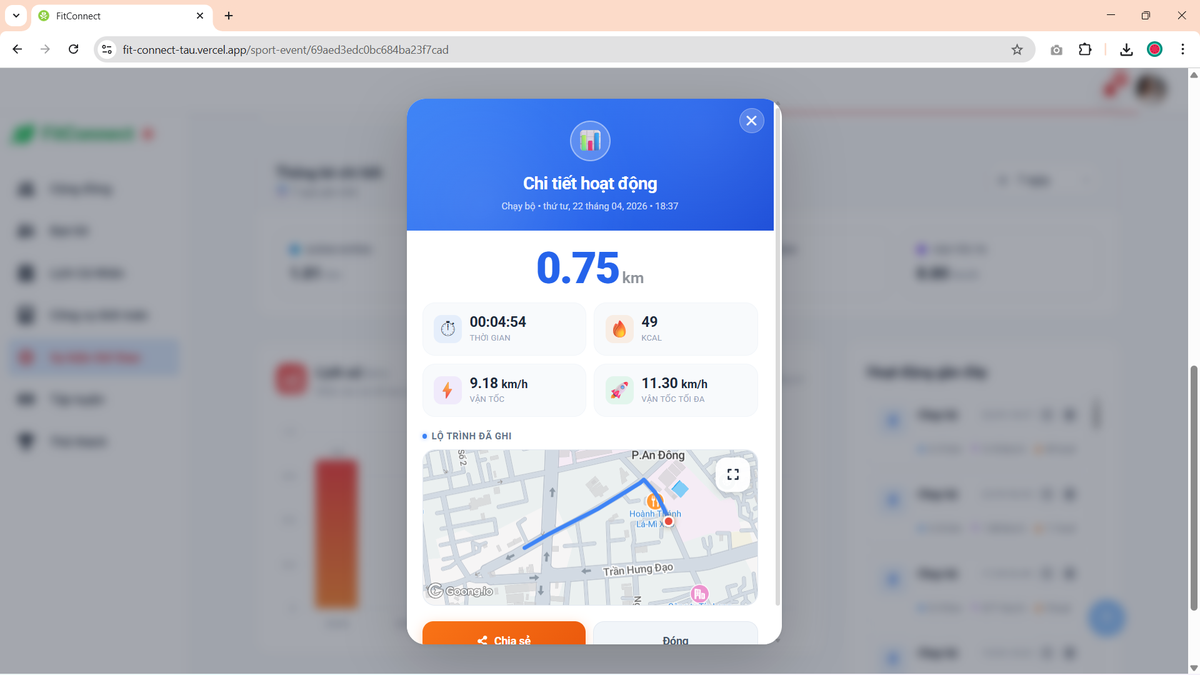
\includegraphics[width=0.60\textwidth]{Images/IMG/nhom3/xemhoatdongsukienngoaitroi.png}
    \caption{Người tham gia xem chi tiết hoạt động sự kiện ngoài trời đã ghi nhận}
    \label{fig:impl_se_view_activity_outdoor}
\end{figure}


        \item Người tham gia có thể chia sẻ hoạt động, sau khi chia sẻ hoạt động sẽ được hiển thị trên bài viết cộng đồng.

\begin{figure}[H]
    \centering
    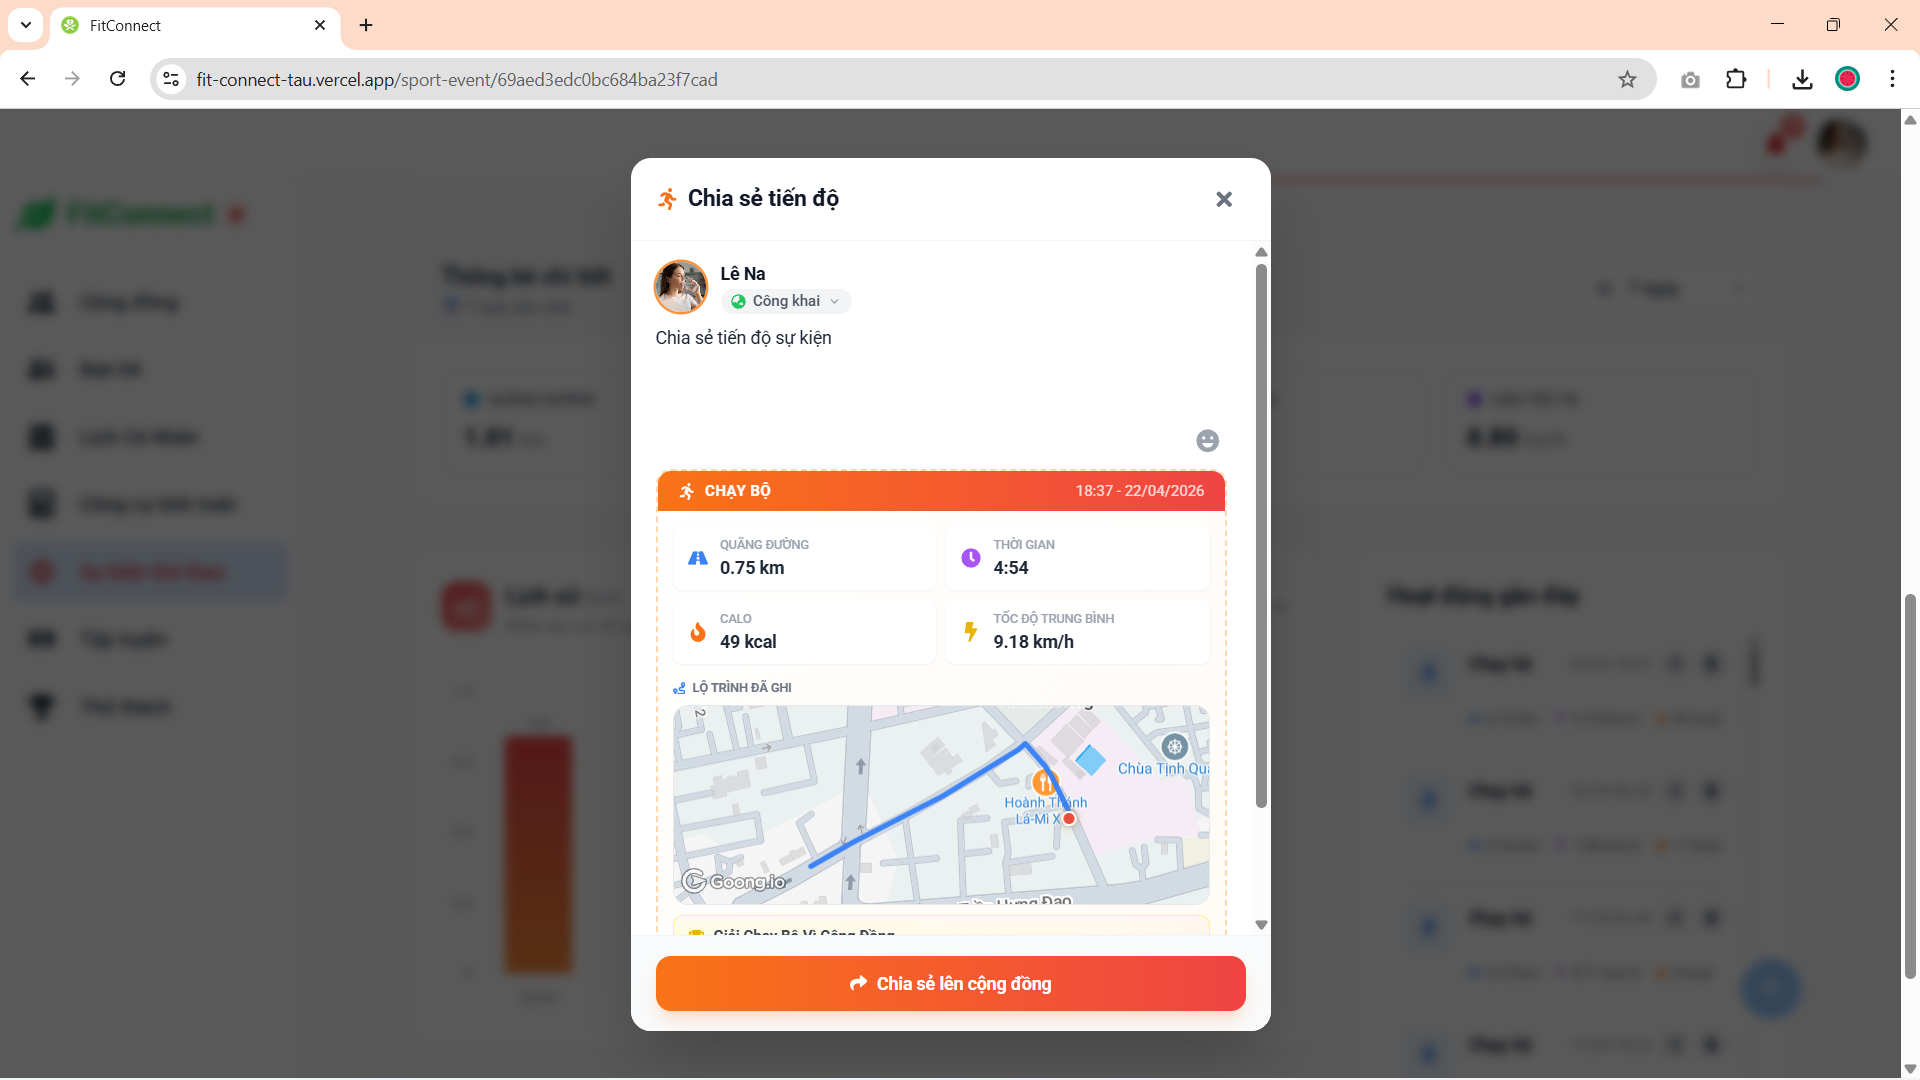
\includegraphics[width=0.60\textwidth]{Images/IMG/nhom3/chiasehoatdongngoaitroi.png}
    \caption{Người tham gia chia sẻ hoạt động ngoài trời lên bảng tin cộng đồng}
    \label{fig:impl_se_share_activity}
\end{figure}


    \end{itemize}
\end{itemize}

\textbf{Tiến độ sự kiện Trong nhà:}
\begin{itemize}
    \item Đối với sự kiện Trong nhà, người tham gia có thể nhấn vào tab Tiến độ và xem được thông tin tiến độ tổng quan bao gồm: phần trăm hoàn thành mục tiêu cá nhân (kcal), tiến độ đạt được, thống kê chi tiết (thời gian, calories, lần tham gia, thời gian trung bình/buổi), biểu đồ lịch sử và danh sách lịch sử buổi học.

\begin{figure}[H]
    \centering
    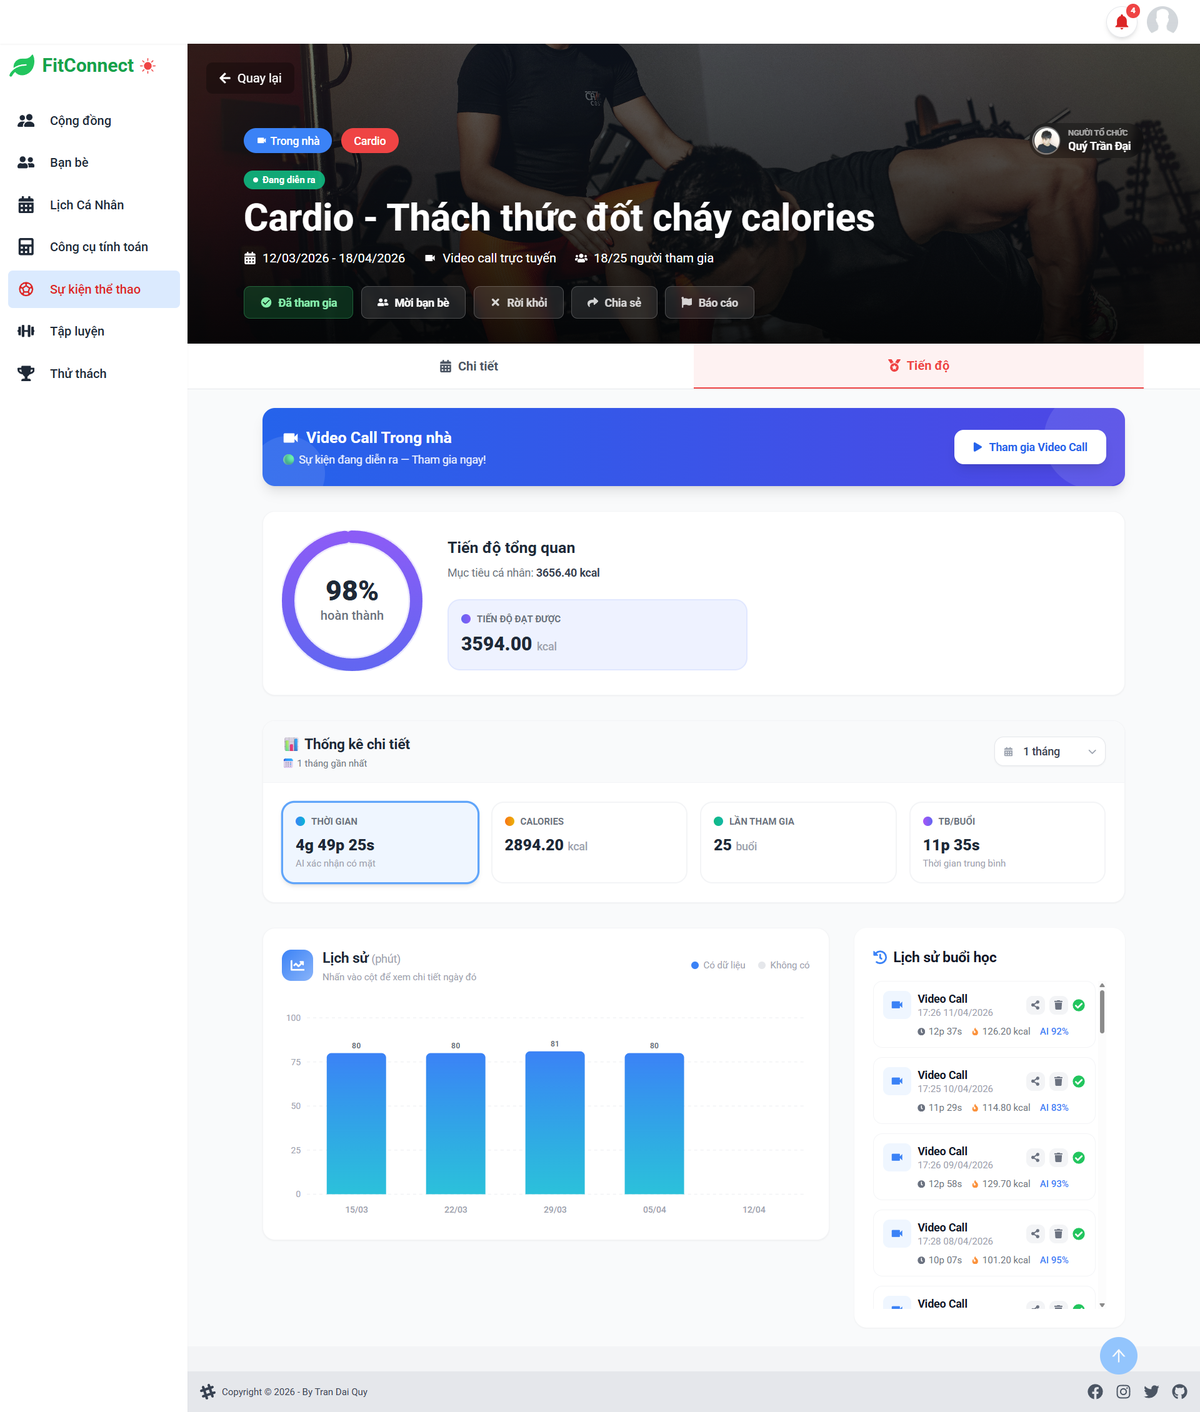
\includegraphics[width=0.60\textwidth]{Images/IMG/nhom3/tiendosukientrongnha.png}
    \caption{Người tham gia xem tiến độ sự kiện trong nhà}
    \label{fig:impl_se_progress_indoor}
\end{figure}


    \item Người tham gia có thể tham gia Video Call sự kiện để tập luyện trực tuyến cùng nhau.
    \begin{itemize}
        \item Khi người tham gia nhấn Tham gia Video Call, hệ thống sẽ hiển thị giao diện video call trực tuyến bao gồm: video của bản thân và các thành viên khác, thời gian tham gia, thời gian thực tế (được AI xác nhận có mặt), calories đã đốt, trạng thái AI đang theo dõi, và các nút chức năng (Tắt mic, Tắt cam, Chia sẻ màn hình, Kết thúc).

\begin{figure}[H]
    \centering
    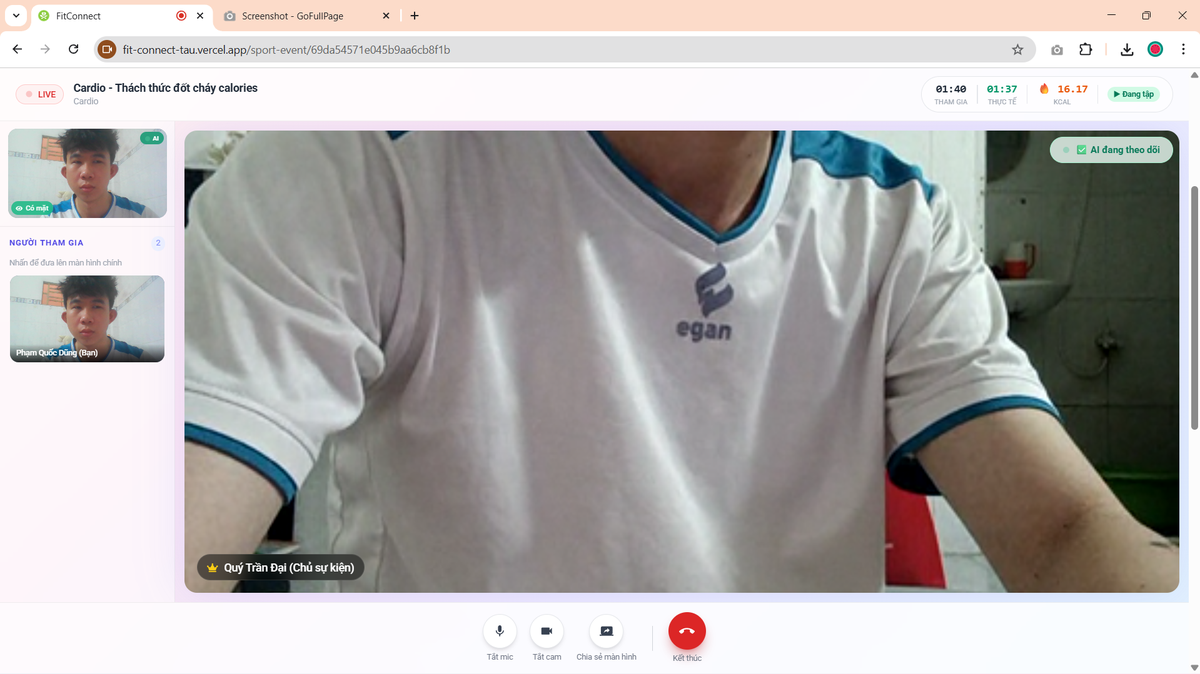
\includegraphics[width=0.60\textwidth]{Images/IMG/nhom3/thamgiavideocall.png}
    \caption{Người tham gia tham gia sự kiện qua Video Call với AI theo dõi}
    \label{fig:impl_se_videocall}
\end{figure}


        \item Nếu người tham gia tắt camera, AI Tracking sẽ nhận diện và tạm dừng ghi nhận thời gian thực tế, đồng thời hiển thị trạng thái ``Vắng'' trên giao diện.

\begin{figure}[H]
    \centering
    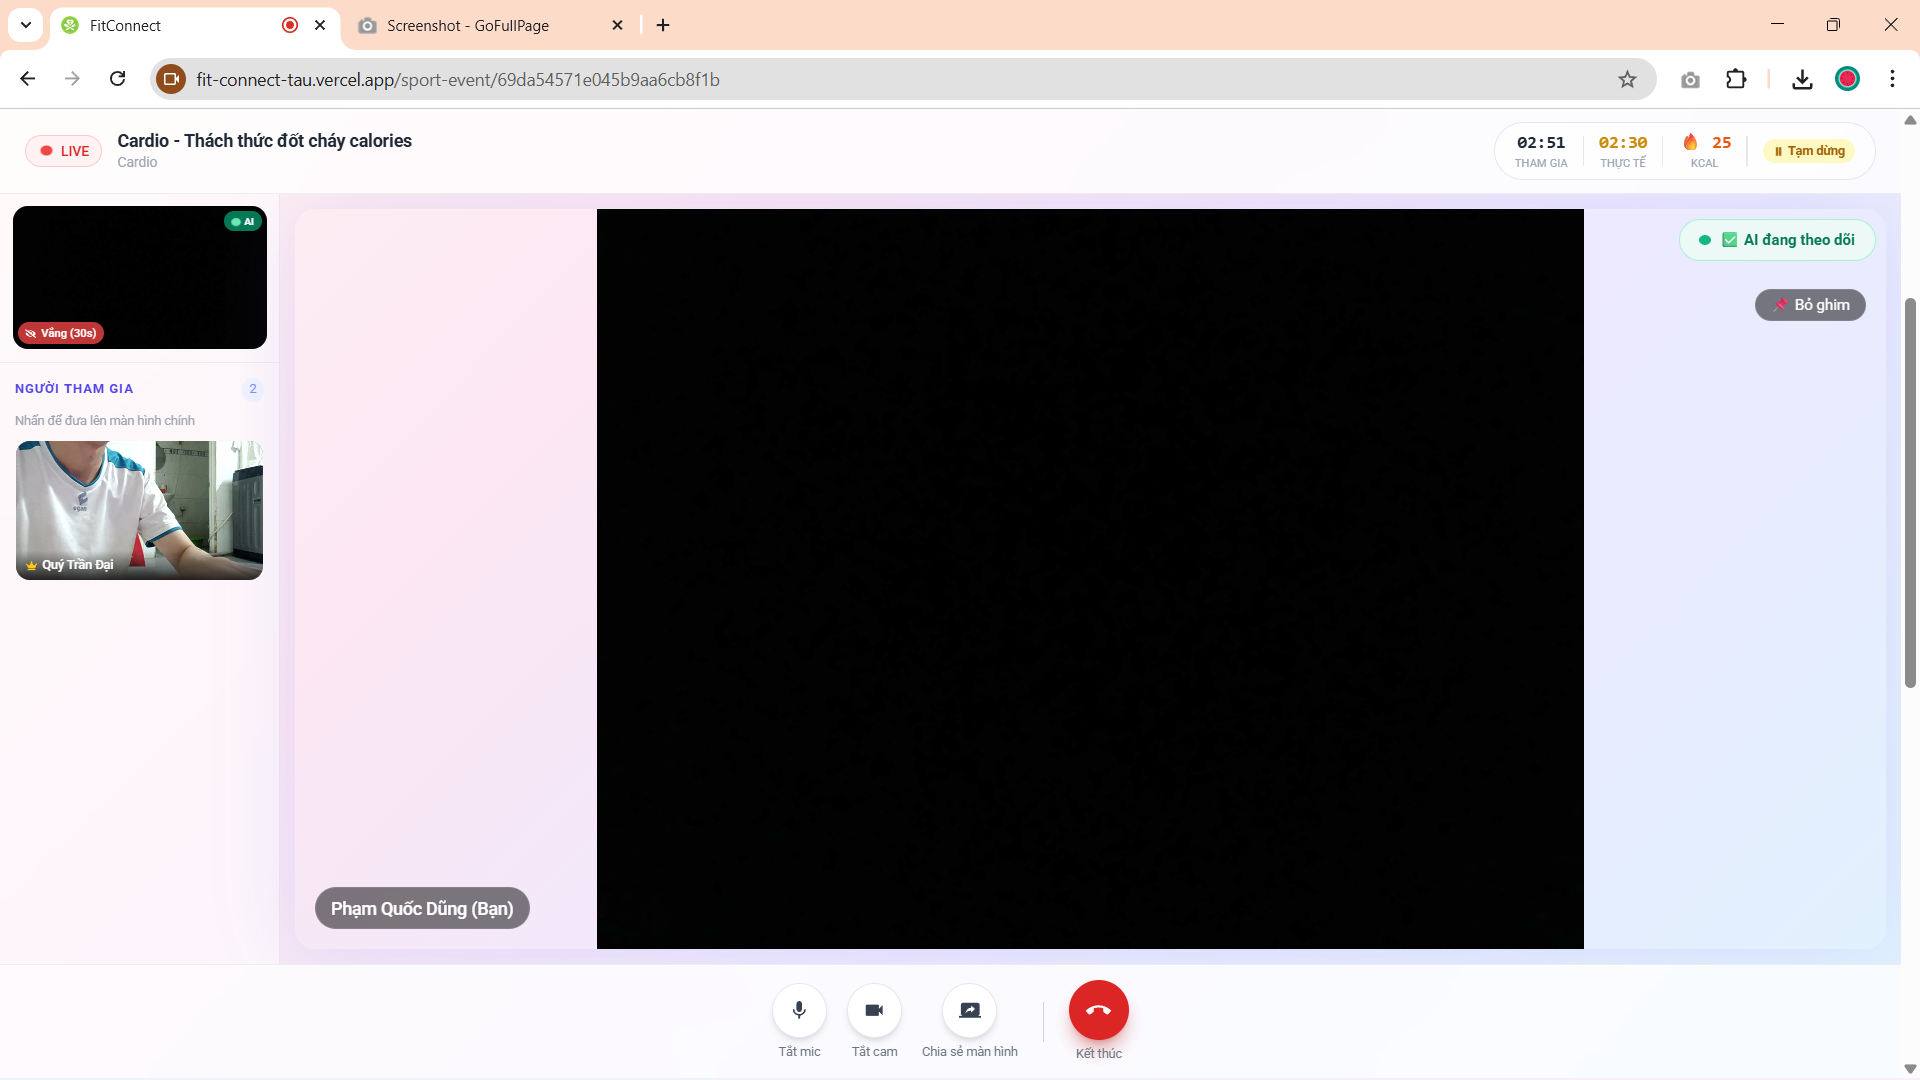
\includegraphics[width=0.60\textwidth]{Images/IMG/nhom3/checameraAInhandientamdung.png}
    \caption{Hệ thống AI nhận diện người tham gia tắt camera và tạm dừng ghi nhận}
    \label{fig:impl_se_ai_pause}
\end{figure}


        \item Sau khi nhấn Kết thúc Video Call, hệ thống tổng hợp thông tin hoạt động: thời gian tham gia, thời gian AI xác nhận có mặt và calories đã đốt (kcal). Người tham gia có thể chia sẻ hoạt động lên bảng tin cộng đồng.

    \end{itemize}
\end{itemize}

\subsubsection{Luồng thao tác quản trị sự kiện (Góc độ Quản trị viên)}
\begin{itemize}
    \item Quản trị viên truy cập trang Kiểm duyệt sự kiện thể thao, hệ thống hiển thị danh sách sự kiện bị báo cáo bao gồm thông tin: người tạo sự kiện, tên sự kiện, số báo cáo, người báo cáo, nội dung báo cáo và các hành động (xem chi tiết, giữ sự kiện, gỡ sự kiện).

\begin{figure}[H]
    \centering
    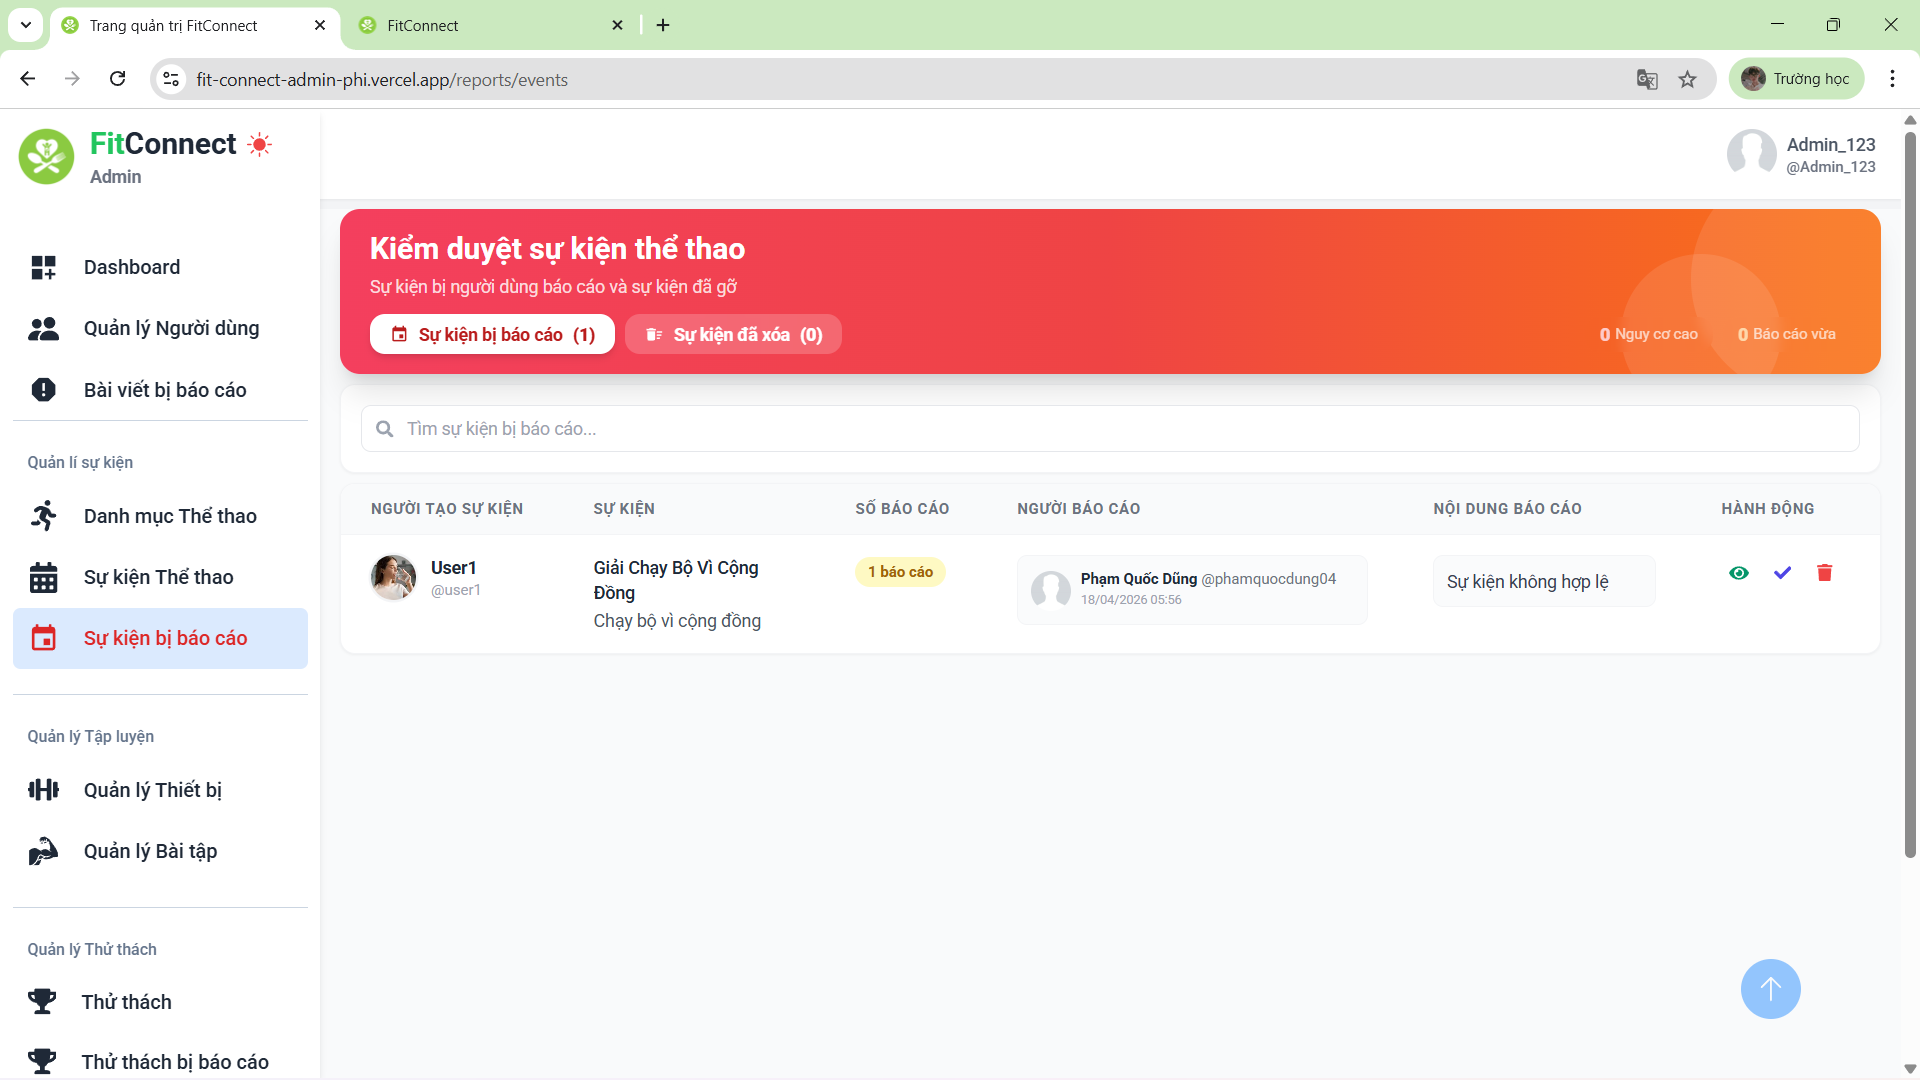
\includegraphics[width=0.60\textwidth]{Images/IMG/nhom3/adminxemdanhsachsukienbaocao.png}
    \caption{Quản trị viên xem danh sách sự kiện bị báo cáo}
    \label{fig:impl_se_admin_list}
\end{figure}


    \item Quản trị viên có thể nhấn xem chi tiết để xem thông tin sự kiện bị báo cáo bao gồm: tên sự kiện, trạng thái, thời gian diễn ra, số người tham gia, danh sách người báo cáo, thông tin sự kiện (thể loại, loại sự kiện, số người tối đa, địa điểm chi tiết).

\begin{figure}[H]
    \centering
    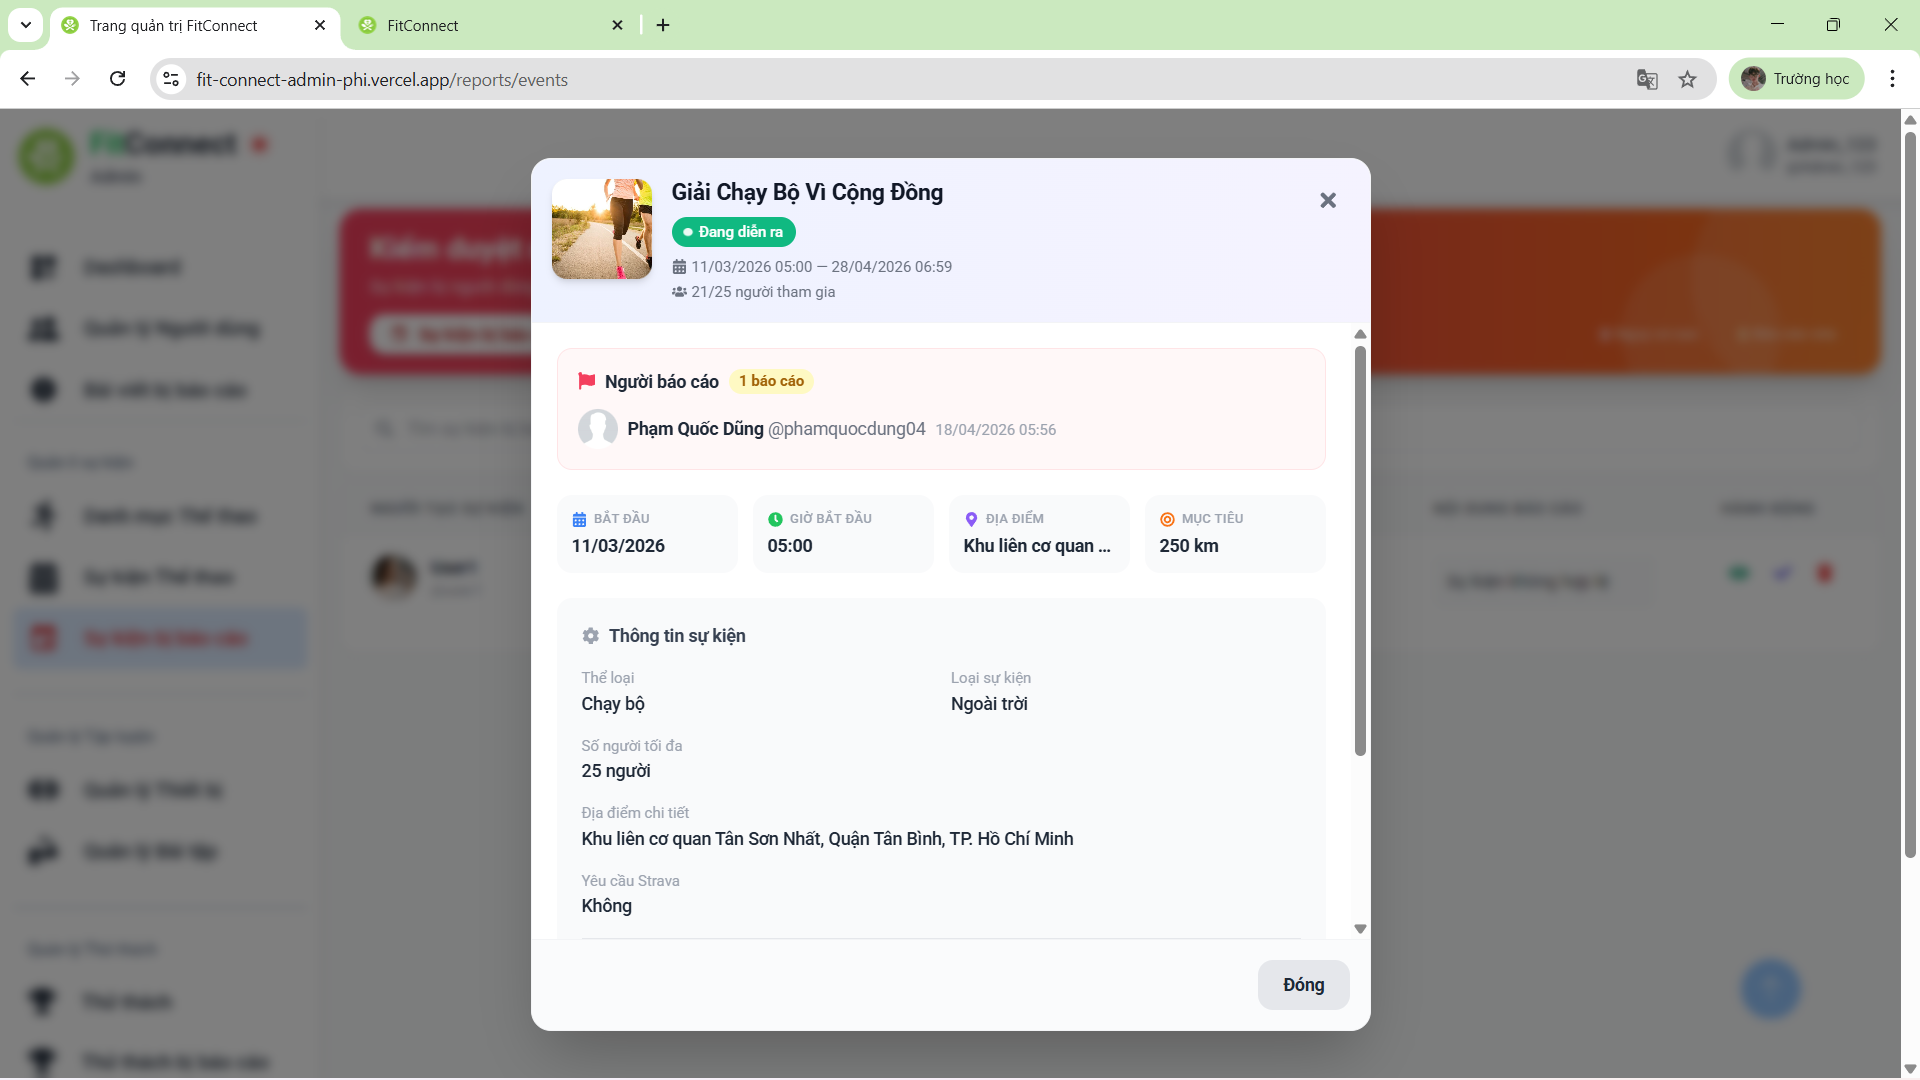
\includegraphics[width=0.60\textwidth]{Images/IMG/nhom3/adminxemthongtinsukienbibaoca.png}
    \caption{Quản trị viên xem thông tin chi tiết sự kiện bị báo cáo}
    \label{fig:impl_se_admin_view}
\end{figure}


    \item Dựa trên xác minh, Admin \textbf{Giữ sự kiện} (xóa toàn bộ báo cáo, sự kiện tiếp tục hoạt động) hoặc \textbf{Gỡ sự kiện} (ẩn khỏi hệ thống, chuyển sang tab ``Đã xóa''). Sự kiện đã gỡ có thể được khôi phục trở lại bất kỳ lúc nào.

\begin{figure}[H]
    \centering
    \begin{subfigure}[b]{0.47\textwidth}
        \centering
        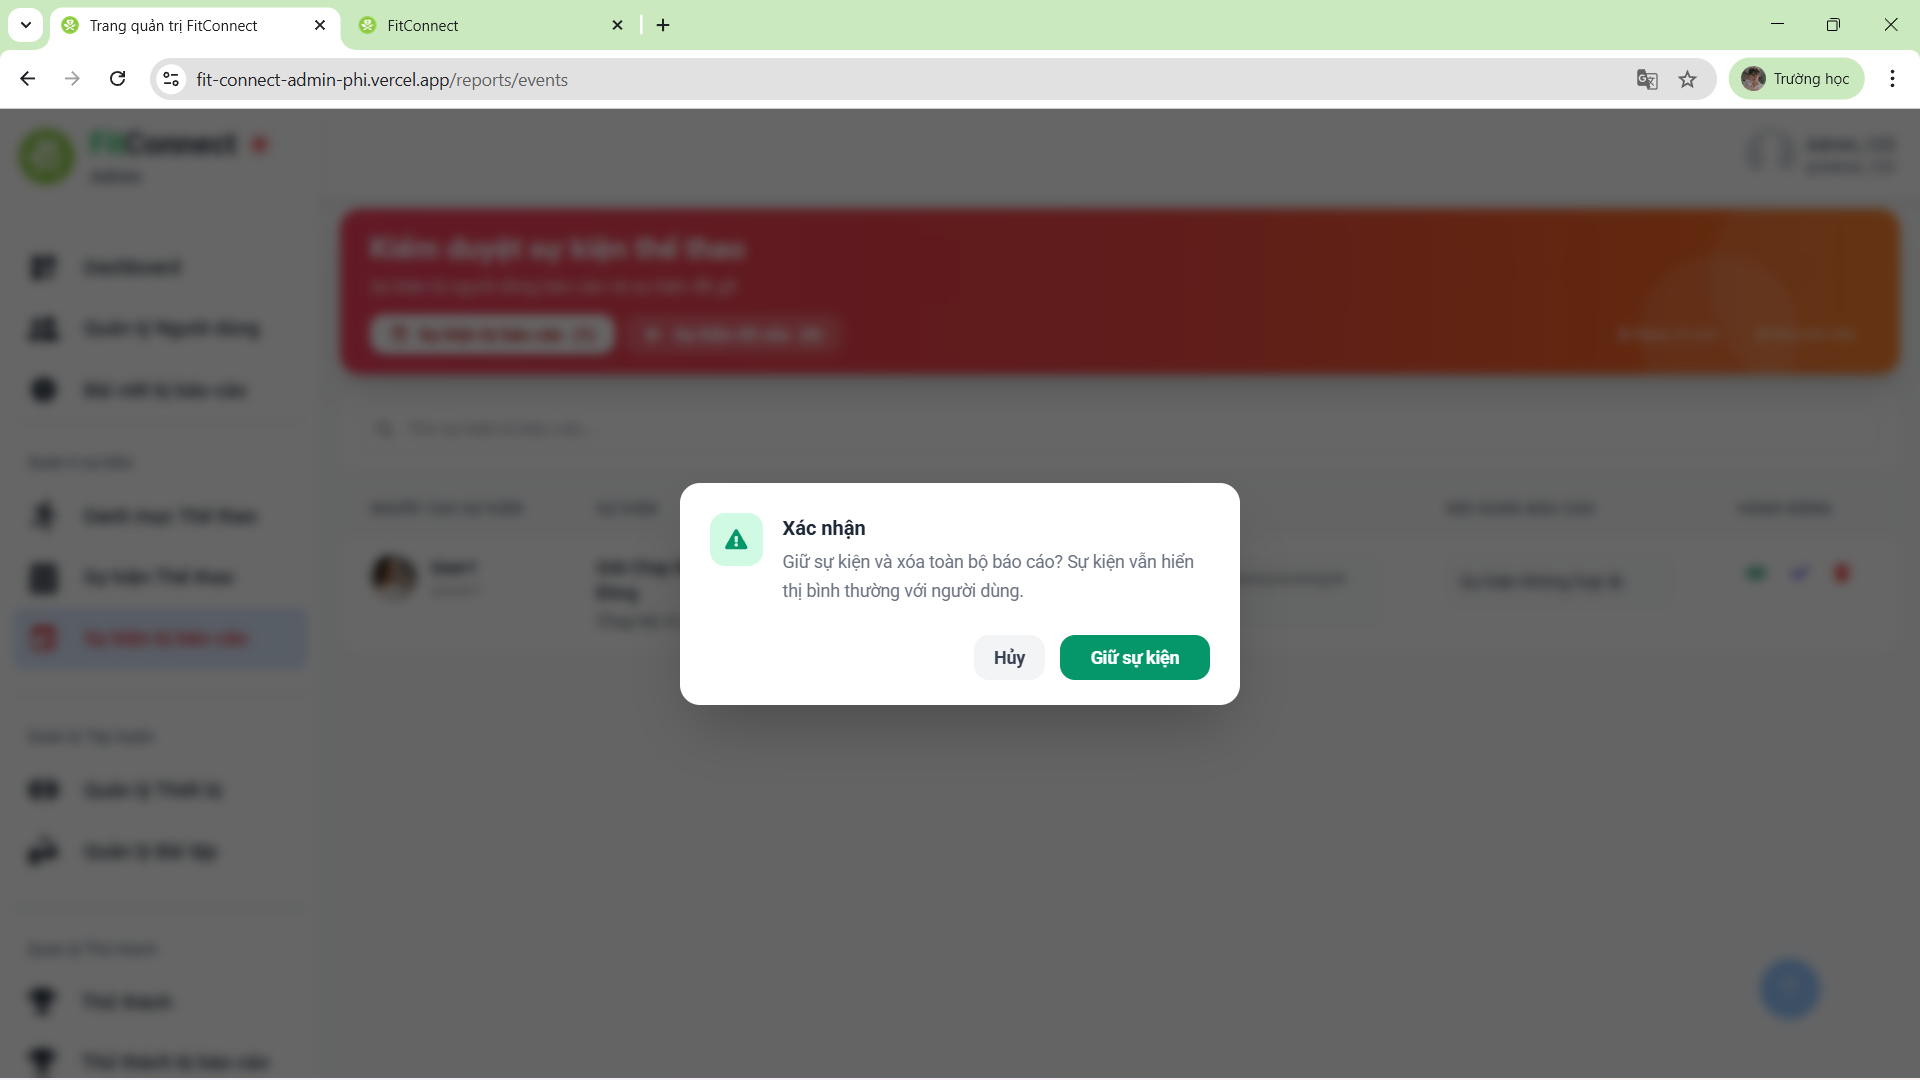
\includegraphics[width=\textwidth]{Images/IMG/nhom3/admingiusukien.png}
        \caption{Xác nhận giữ sự kiện hợp lệ}
        \label{fig:impl_se_admin_keep}
    \end{subfigure}
    \hfill
    \begin{subfigure}[b]{0.47\textwidth}
        \centering
        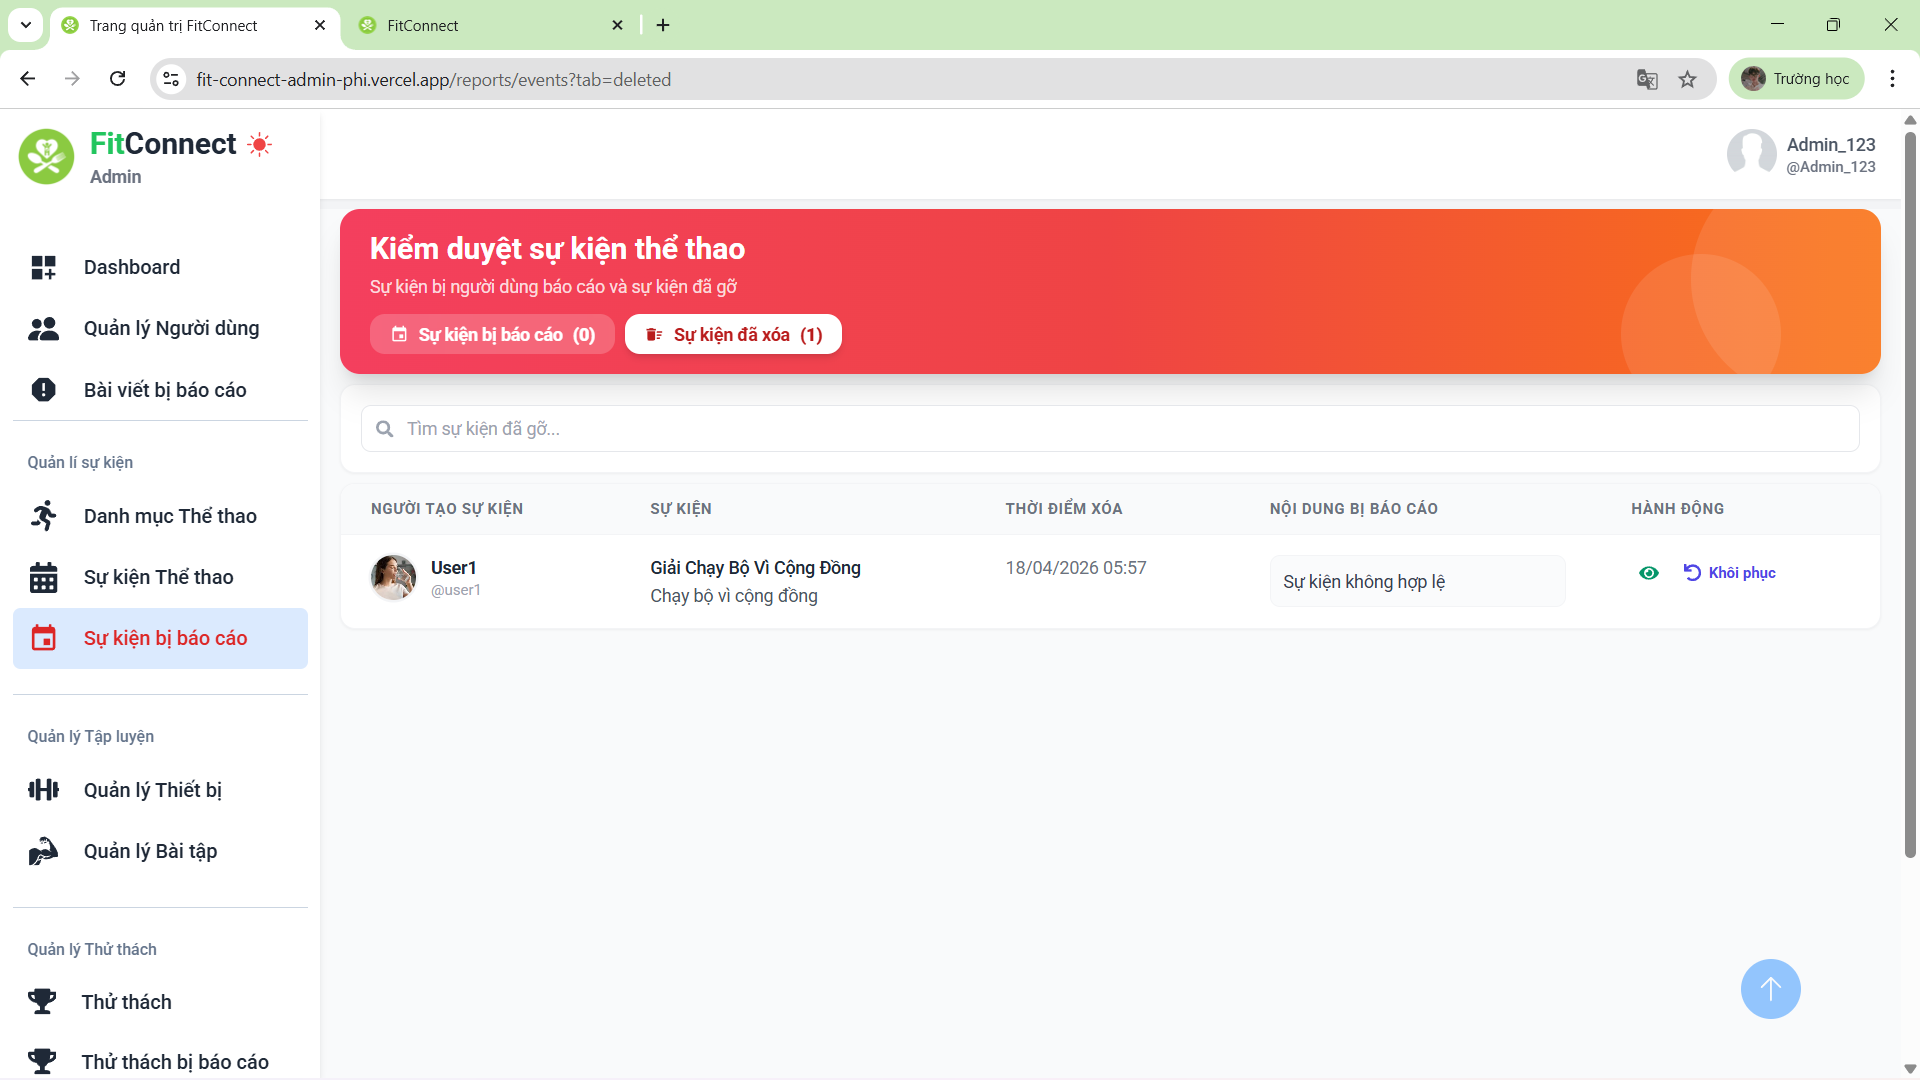
\includegraphics[width=\textwidth]{Images/IMG/nhom3/adminxemsukienbixoa.png}
        \caption{Danh sách sự kiện đã xóa và tùy chọn khôi phục}
        \label{fig:impl_se_admin_deleted_list}
    \end{subfigure}
    \vspace{0.3em}
    \caption{Xử lý kiểm duyệt sự kiện bị báo cáo và quản lý kho sự kiện đã xóa}
    \label{fig:impl_se_admin_moderation}
\end{figure}

\end{itemize}

\subsection{Nhóm tính năng Thử thách cộng đồng}
\label{subsec:impl_challenge}

Nhóm tính năng Thử thách cộng đồng cho phép người dùng tạo và tham gia các thử thách hàng ngày nhằm duy trì thói quen luyện tập và ăn uống lành mạnh. Hệ thống hỗ trợ ba loại thử thách: Ngoài trời (chạy bộ, đạp xe, leo núi,...) với tiến độ ghi nhận qua GPS Tracking, Ăn uống (ăn sạch, giảm cân, detox,...) với tiến độ ghi nhận qua chụp ảnh bữa ăn, và Thể dục (Workout, tập gym,...) với tiến độ ghi nhận qua xác nhận hoàn thành. Mỗi thử thách đặt mục tiêu theo ngày, và người tham gia cần hoàn thành mục tiêu hàng ngày trong suốt thời gian diễn ra thử thách. Ngoài ra, hệ thống còn tích hợp AI để hỗ trợ tạo thử thách tự động qua hai bước đơn giản.

Quy trình hoạt động gồm ba luồng chính:
\begin{itemize}
    \item \textbf{Người dùng (Người tạo thử thách):} Tạo, quản lý thử thách, theo dõi danh sách người tham gia và chỉnh sửa thông tin thử thách.
    \item \textbf{Người dùng (Người tham gia):} Tìm kiếm, tham gia thử thách, ghi tiến độ hàng ngày, chia sẻ và mời bạn bè.
    \item \textbf{Quản trị viên:} Xử lý các thử thách bị báo cáo từ cộng đồng.
\end{itemize}

\subsubsection{Luồng thao tác tạo và quản lý thử thách (Góc độ Người tạo)}
\begin{itemize}
    \item Người dùng truy cập trang Thử thách, hệ thống hiển thị danh sách các thử thách nổi bật dạng banner ở đầu trang, kèm thanh tìm kiếm và bộ lọc theo loại thử thách (Ăn uống, Ngoài trời, Thể dục) và theo danh mục môn thể thao (Cardio, Thiền, Khiêu vũ, Chạy bộ đường dài,...).

\begin{figure}[H]
    \centering
    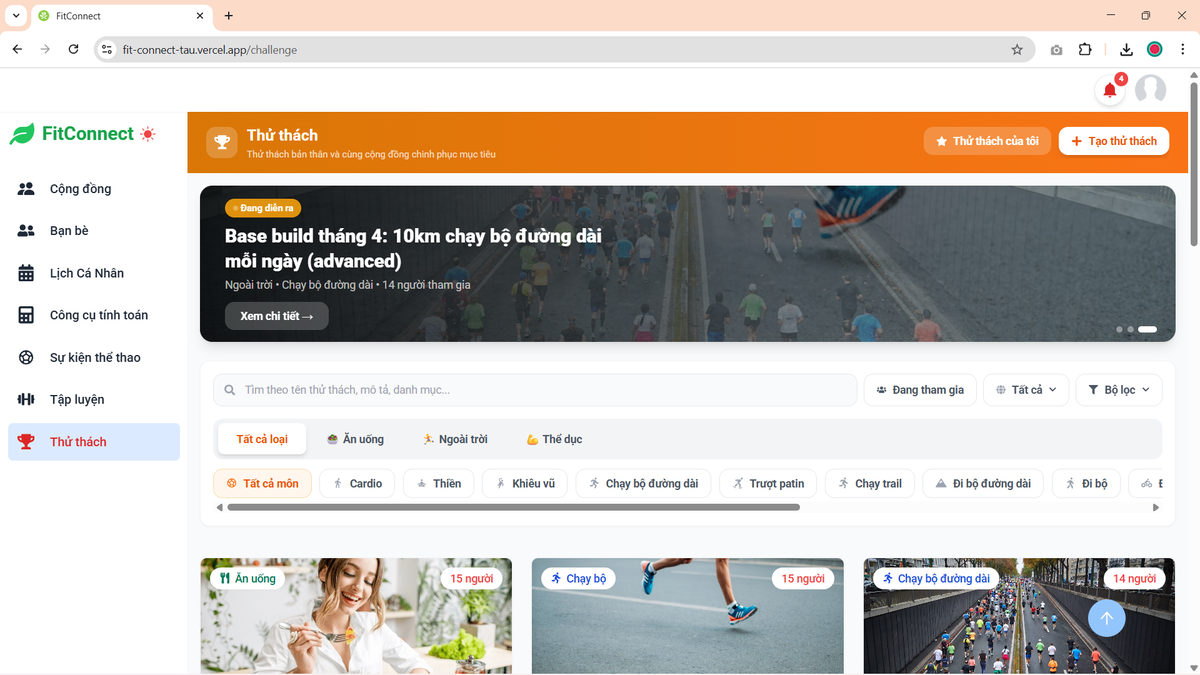
\includegraphics[width=0.60\textwidth]{Images/IMG/nhom4/trangdanhsachthuthach.png}
    \caption{Người dùng xem trang danh sách thử thách cộng đồng}
    \label{fig:impl_ch_list}
\end{figure}


    \item Người dùng nhấn Tạo thử thách mới, hệ thống hiển thị modal tạo thử thách bao gồm các thông tin: loại thử thách (Ngoài trời, Ăn uống, Thể dục), tên thử thách, danh mục hoạt động, mục tiêu mỗi ngày (km hoặc kcal hoặc bữa tùy loại), ngày bắt đầu, ngày kết thúc, hình thức tham gia (Công khai, Bạn bè, Chỉ mình tôi), và hình ảnh. Bên phải có khung Bản xem trước cập nhật real-time khi nhập thông tin.

\begin{figure}[H]
    \centering
    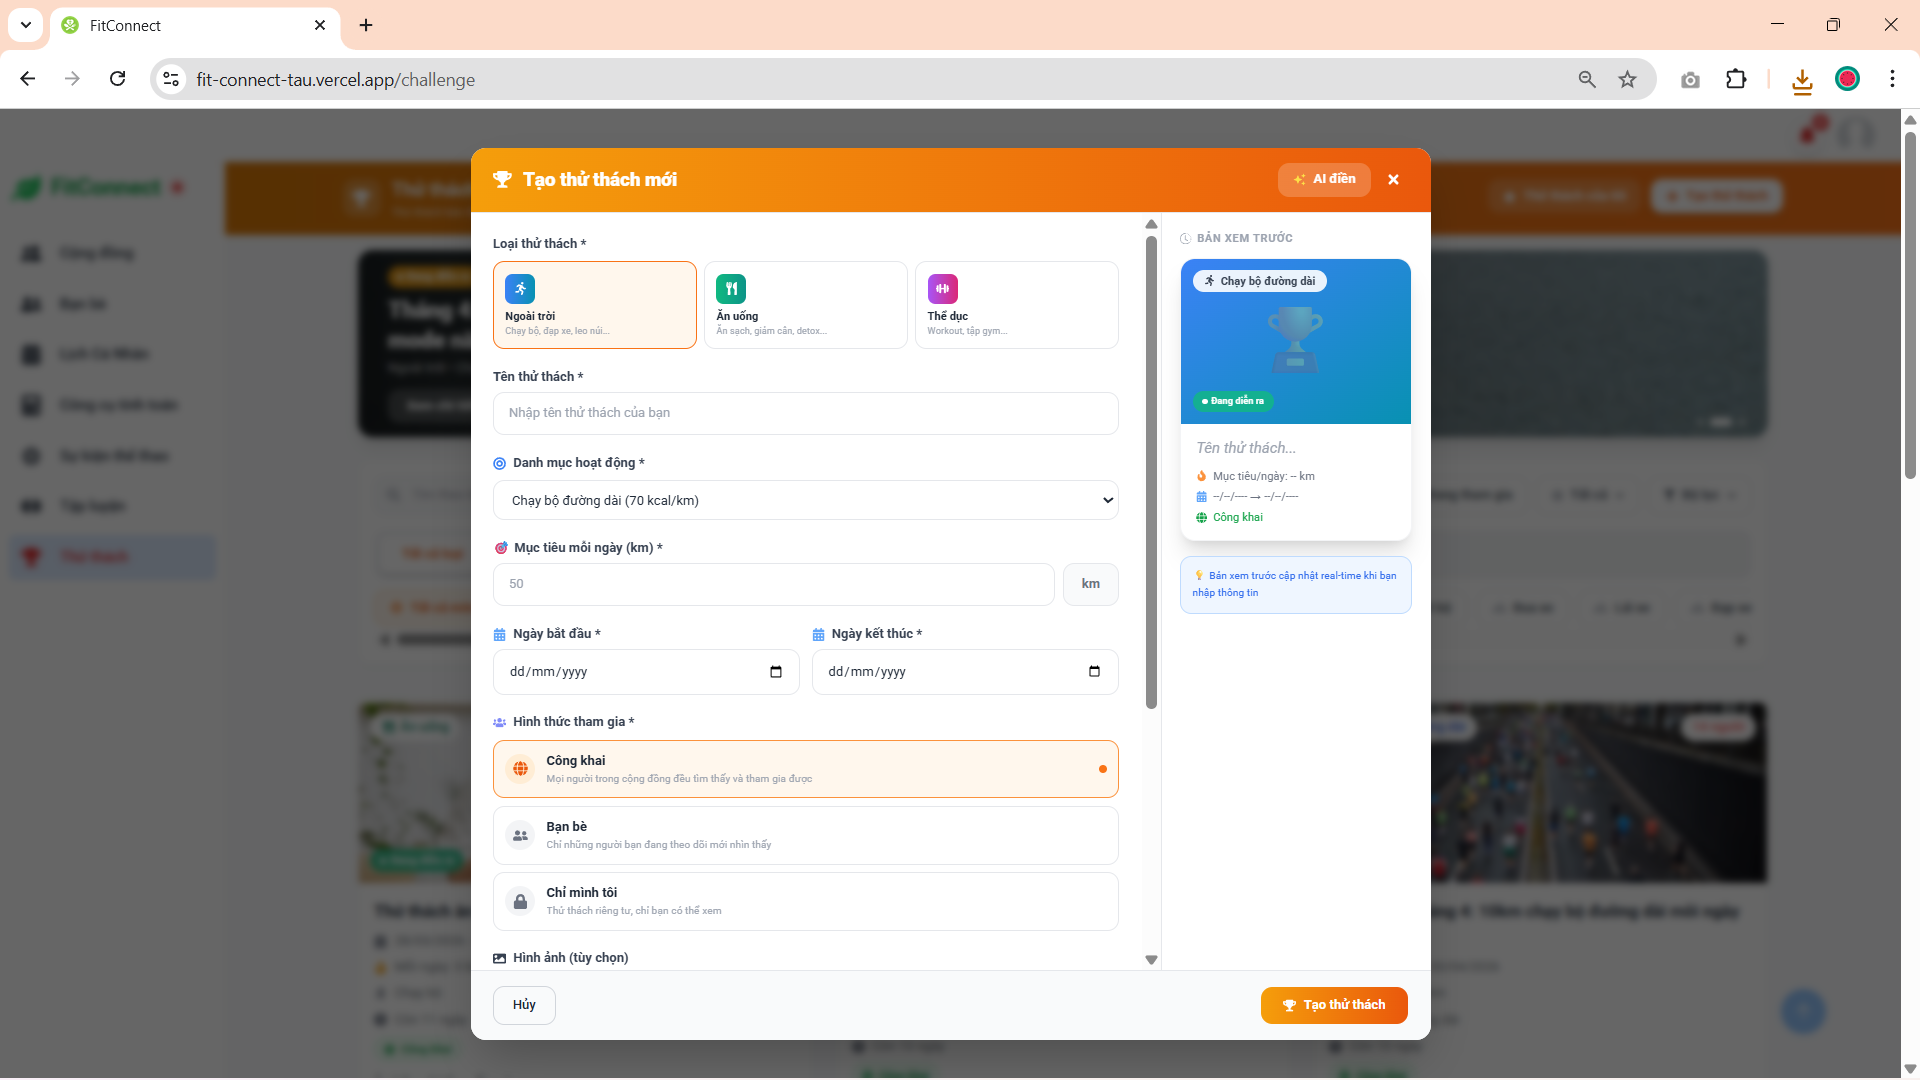
\includegraphics[width=0.60\textwidth]{Images/IMG/nhom4/manhinhtaothuthach.png}
    \caption{Người dùng thao tác tạo thử thách mới}
    \label{fig:impl_ch_create}
\end{figure}


    \item Người dùng có thể dùng tính năng AI tự điền thử thách qua hai bước: Bước 1 -- chọn loại thử thách muốn tạo (Ngoài trời, Ăn uống, Thể dục); Bước 2 -- mô tả ý tưởng thử thách bằng ngôn ngữ tự nhiên (ví dụ: ``Tạo thử thách chạy bộ ngoài trời 1km mỗi ngày từ nay tới hết tháng''), sau đó nhấn Điền ngay để AI tự động điền toàn bộ biểu mẫu.

\begin{figure}[H]
    \centering
    \begin{subfigure}[b]{0.30\textwidth}
        \centering
        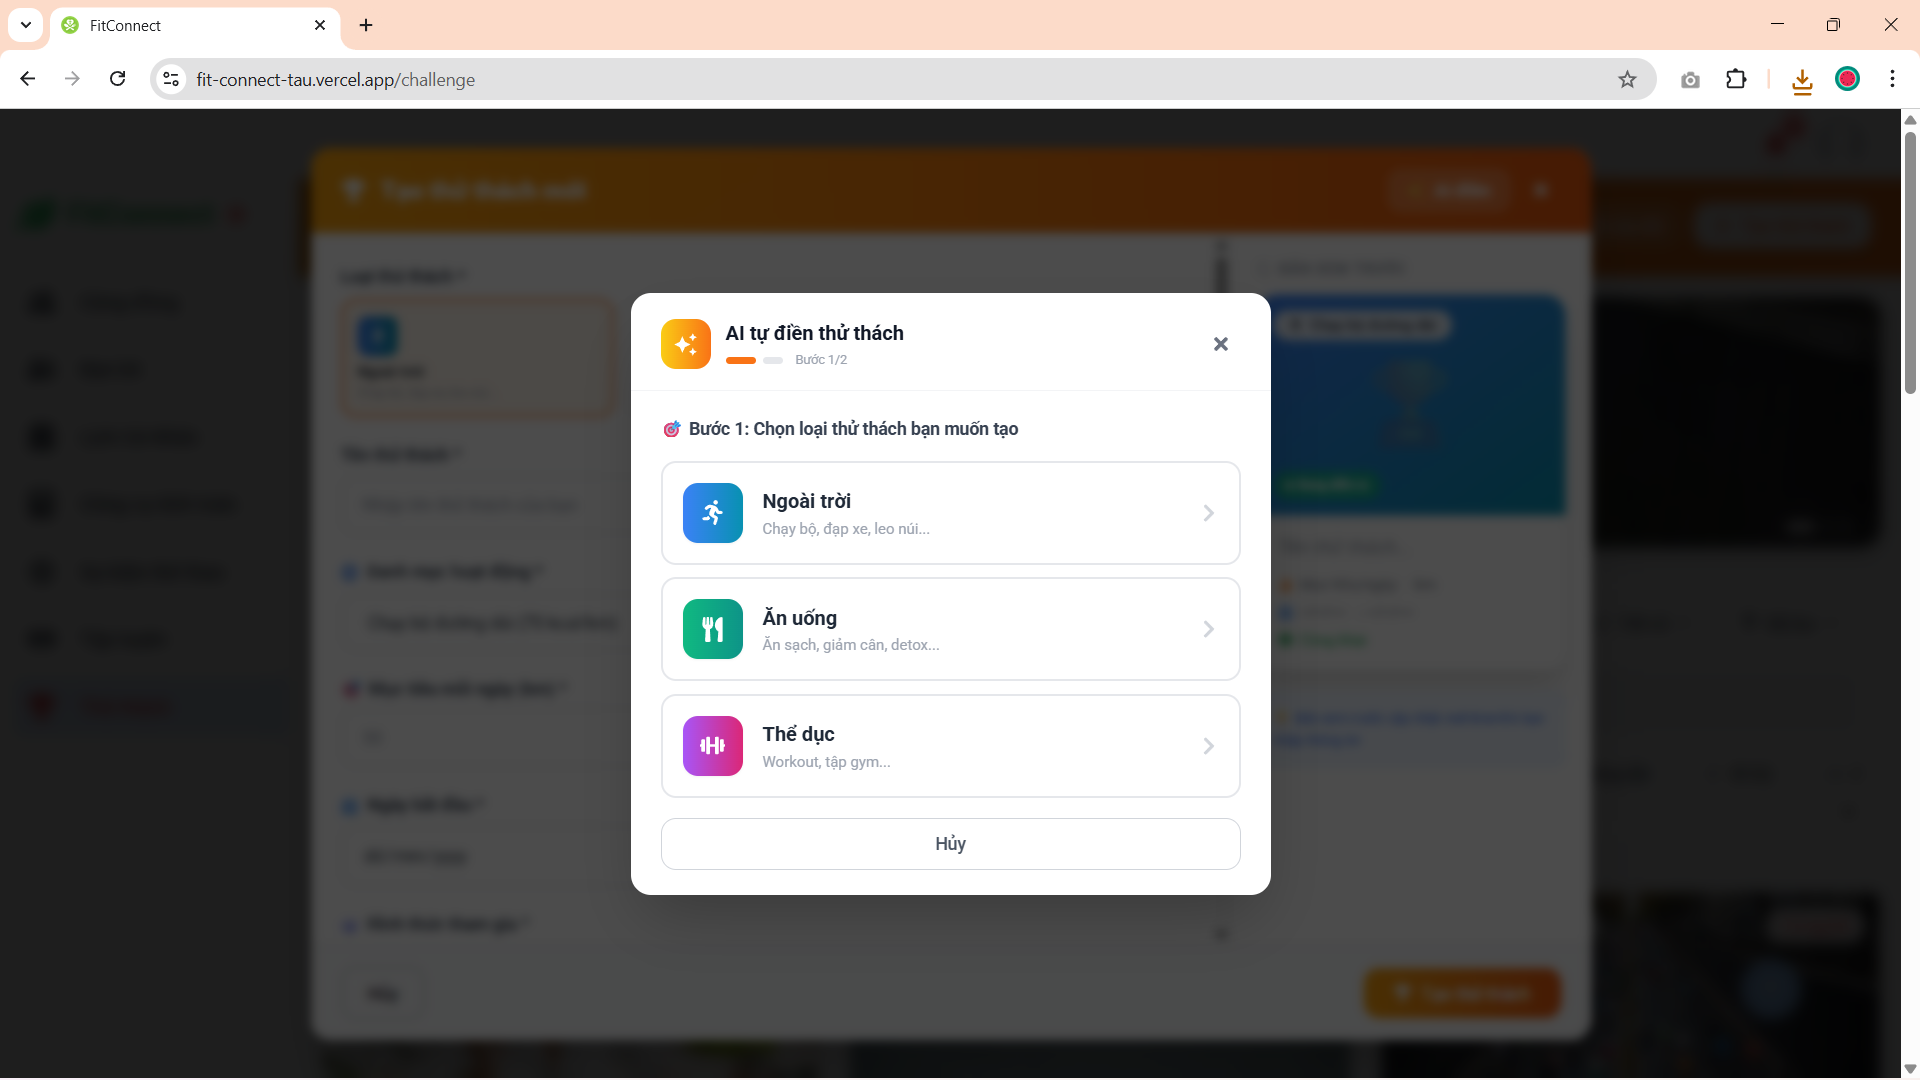
\includegraphics[width=\textwidth]{Images/IMG/nhom4/modalchonloaithuthachtruocAI.png}
        \caption{Hệ thống hiển thị modal AI tự điền thử thách -- Bước 1 chọn loại thử thách}
        \label{fig:impl_ch_ai_step1}
    \end{subfigure}
    \hfill
    \begin{subfigure}[b]{0.30\textwidth}
        \centering
        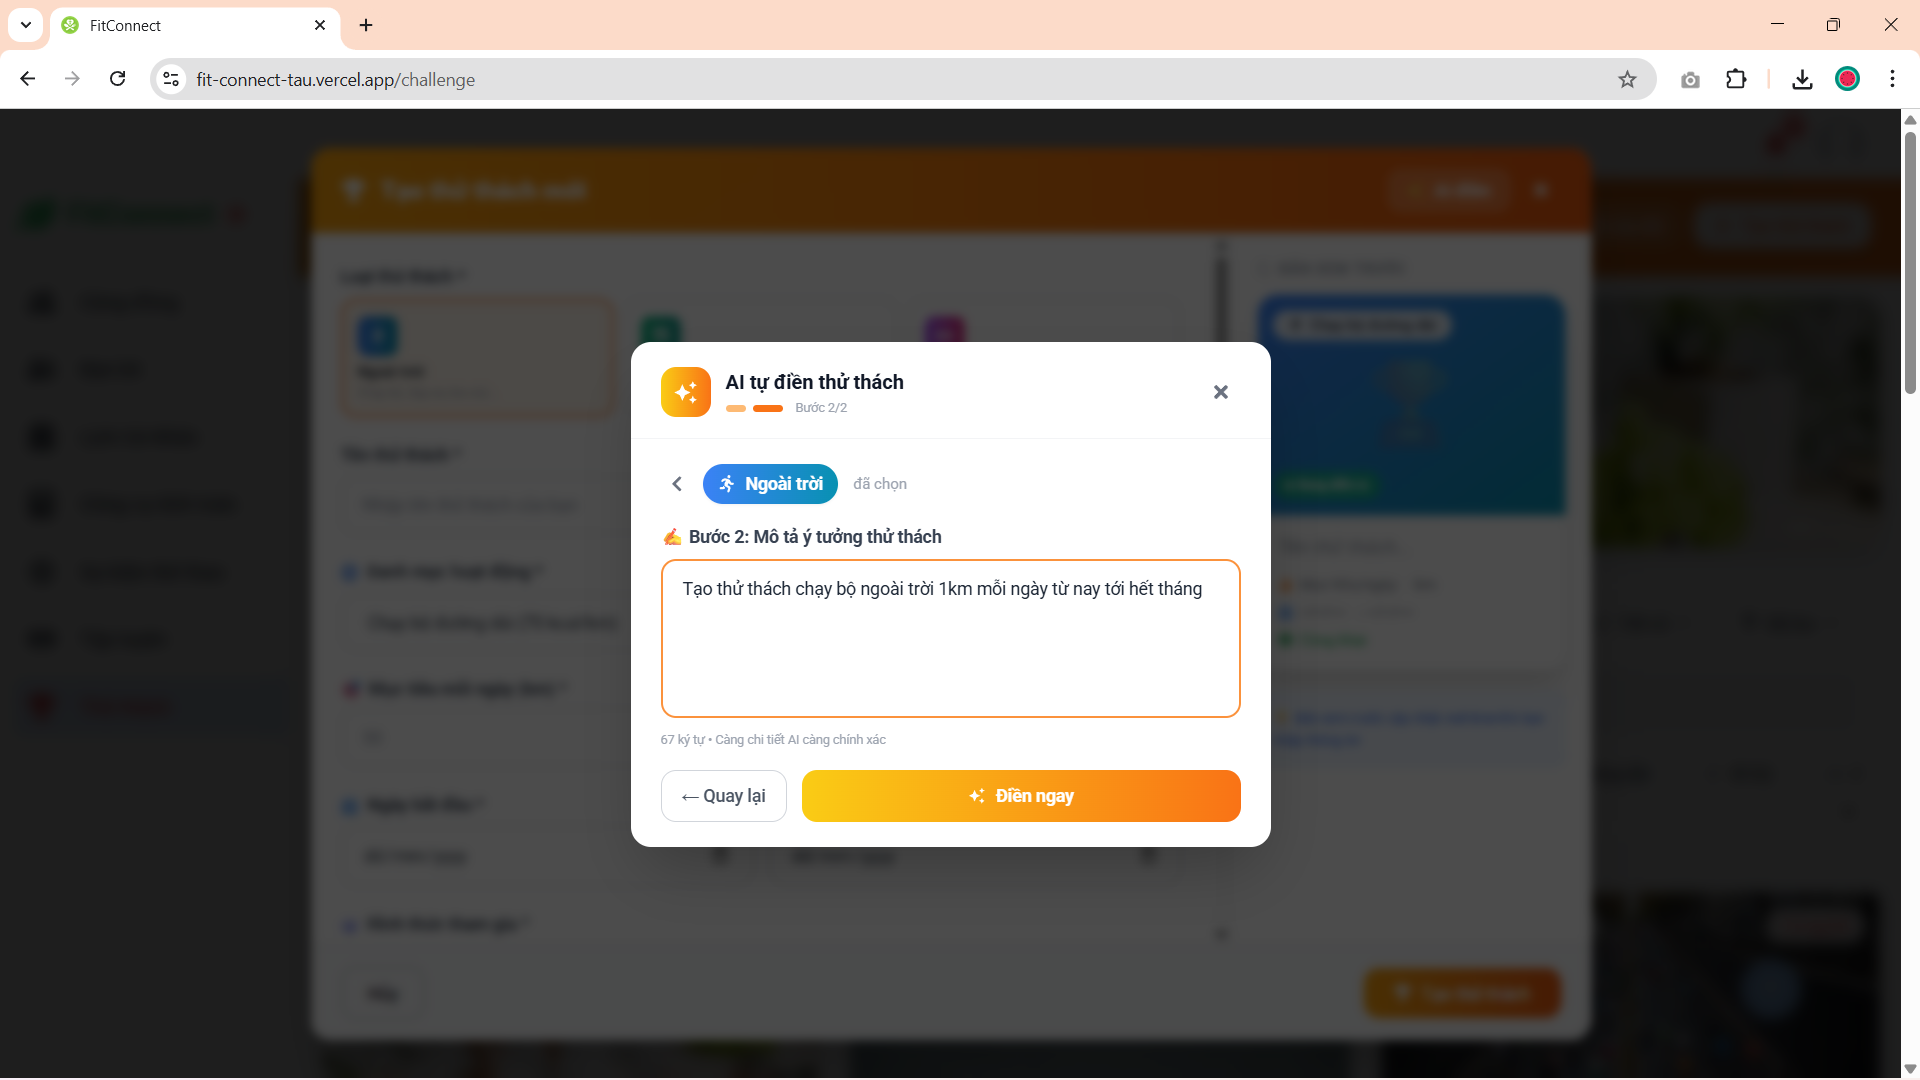
\includegraphics[width=\textwidth]{Images/IMG/nhom4/modalAItaothuthach.png}
        \caption{Hệ thống hiển thị modal AI tự điền thử thách -- Bước 2 mô tả ý tưởng}
        \label{fig:impl_ch_ai_step2}
    \end{subfigure}
    \hfill
    \begin{subfigure}[b]{0.30\textwidth}
        \centering
        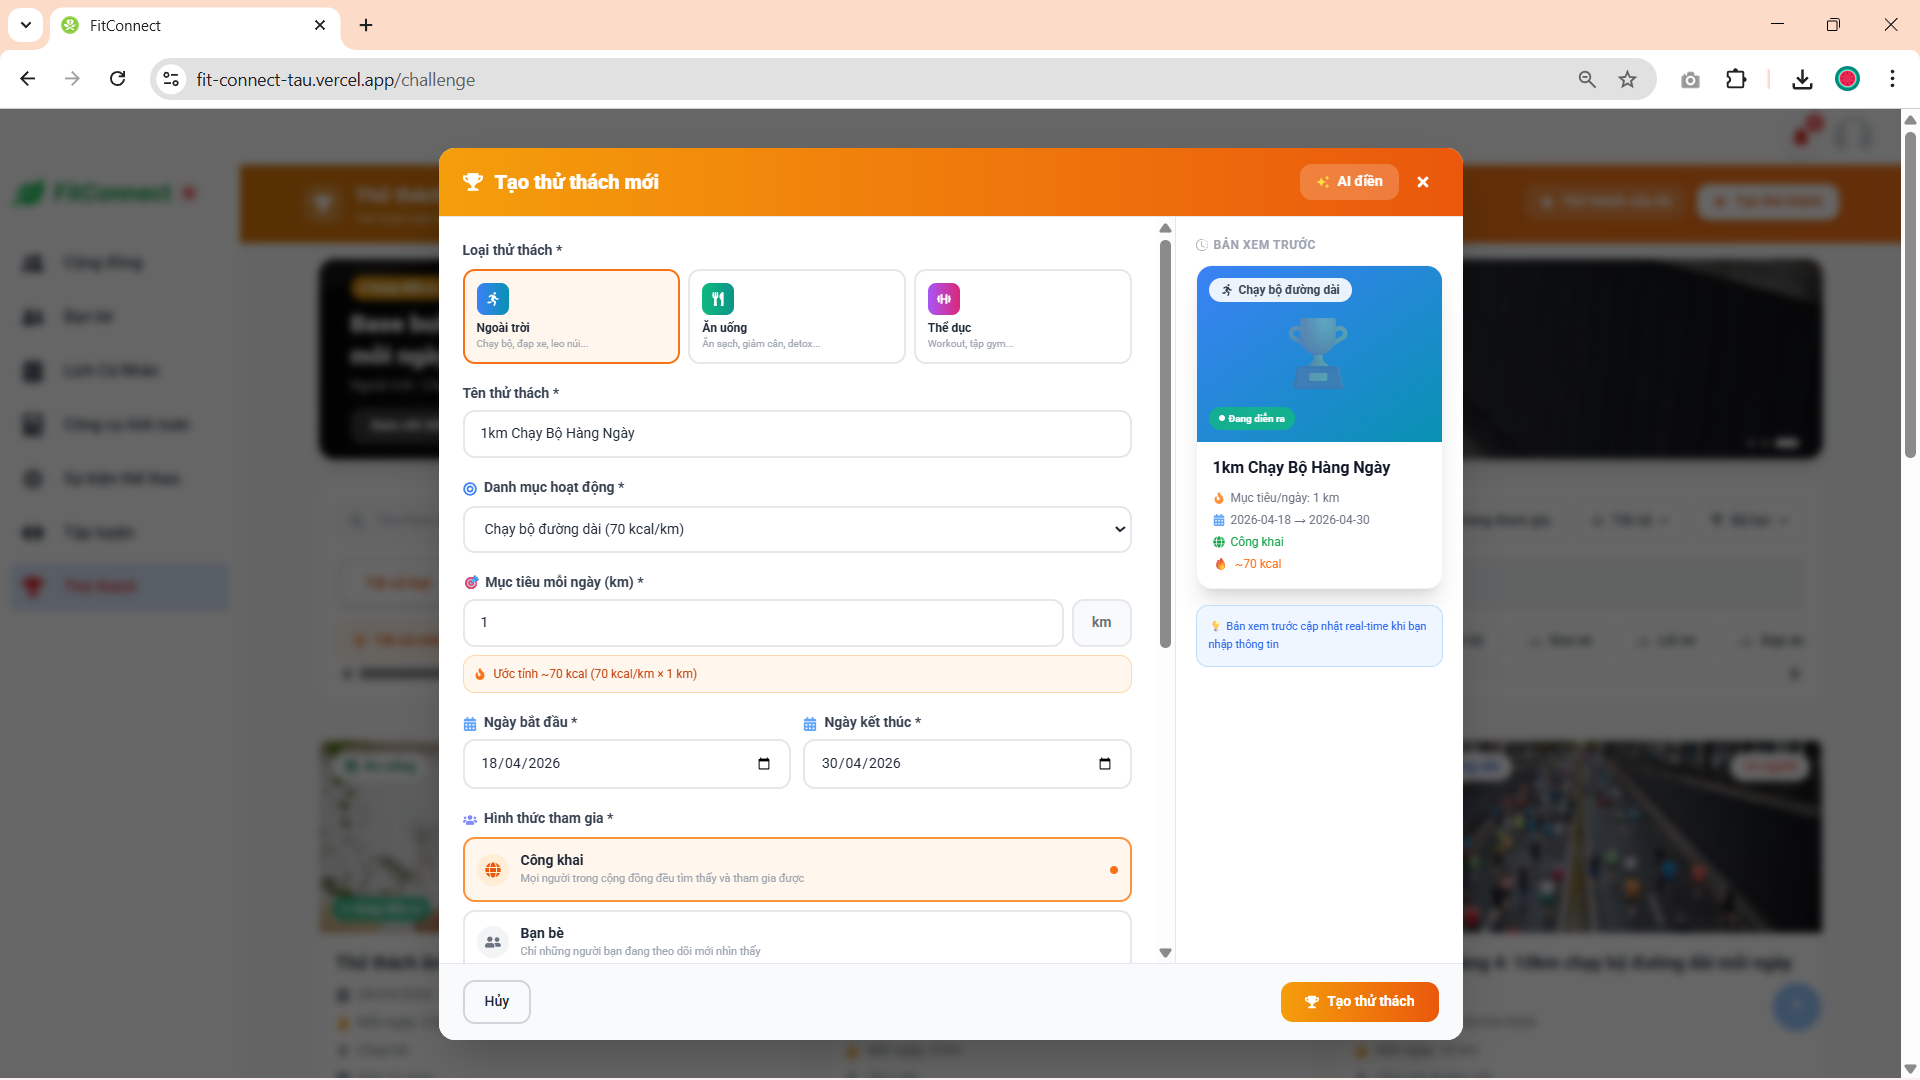
\includegraphics[width=\textwidth]{Images/IMG/nhom4/saukhidungAItaothuthach.png}
        \caption{Hệ thống tự động điền thông tin thử thách sau khi AI xử lý thành công}
        \label{fig:impl_ch_ai_success}
    \end{subfigure}
\end{figure}


    \item Sau khi nhấn Tạo thử thách, hệ thống tự động điều hướng đến trang chi tiết thử thách vừa tạo với đầy đủ thông tin: tên, loại, trạng thái, thời gian, mục tiêu mỗi ngày, số người tham gia và đếm ngược. Người dùng có thể quay lại trang Quản lý Thử thách, nhấn vào ``Thử thách của tôi'' sẽ hiển thị dashboard quản lý với thống kê tổng quan (Tổng đã tạo, Đang diễn ra, Sắp diễn ra, Đã kết thúc) và danh sách thử thách đã tạo cùng thử thách đã tham gia. Bên phải hiển thị thông tin chi tiết của thử thách được chọn với ba tab: Tổng quan, Người tham gia, và Cài đặt.

\begin{figure}[H]
    \centering
    \begin{subfigure}[b]{0.30\textwidth}
        \centering
        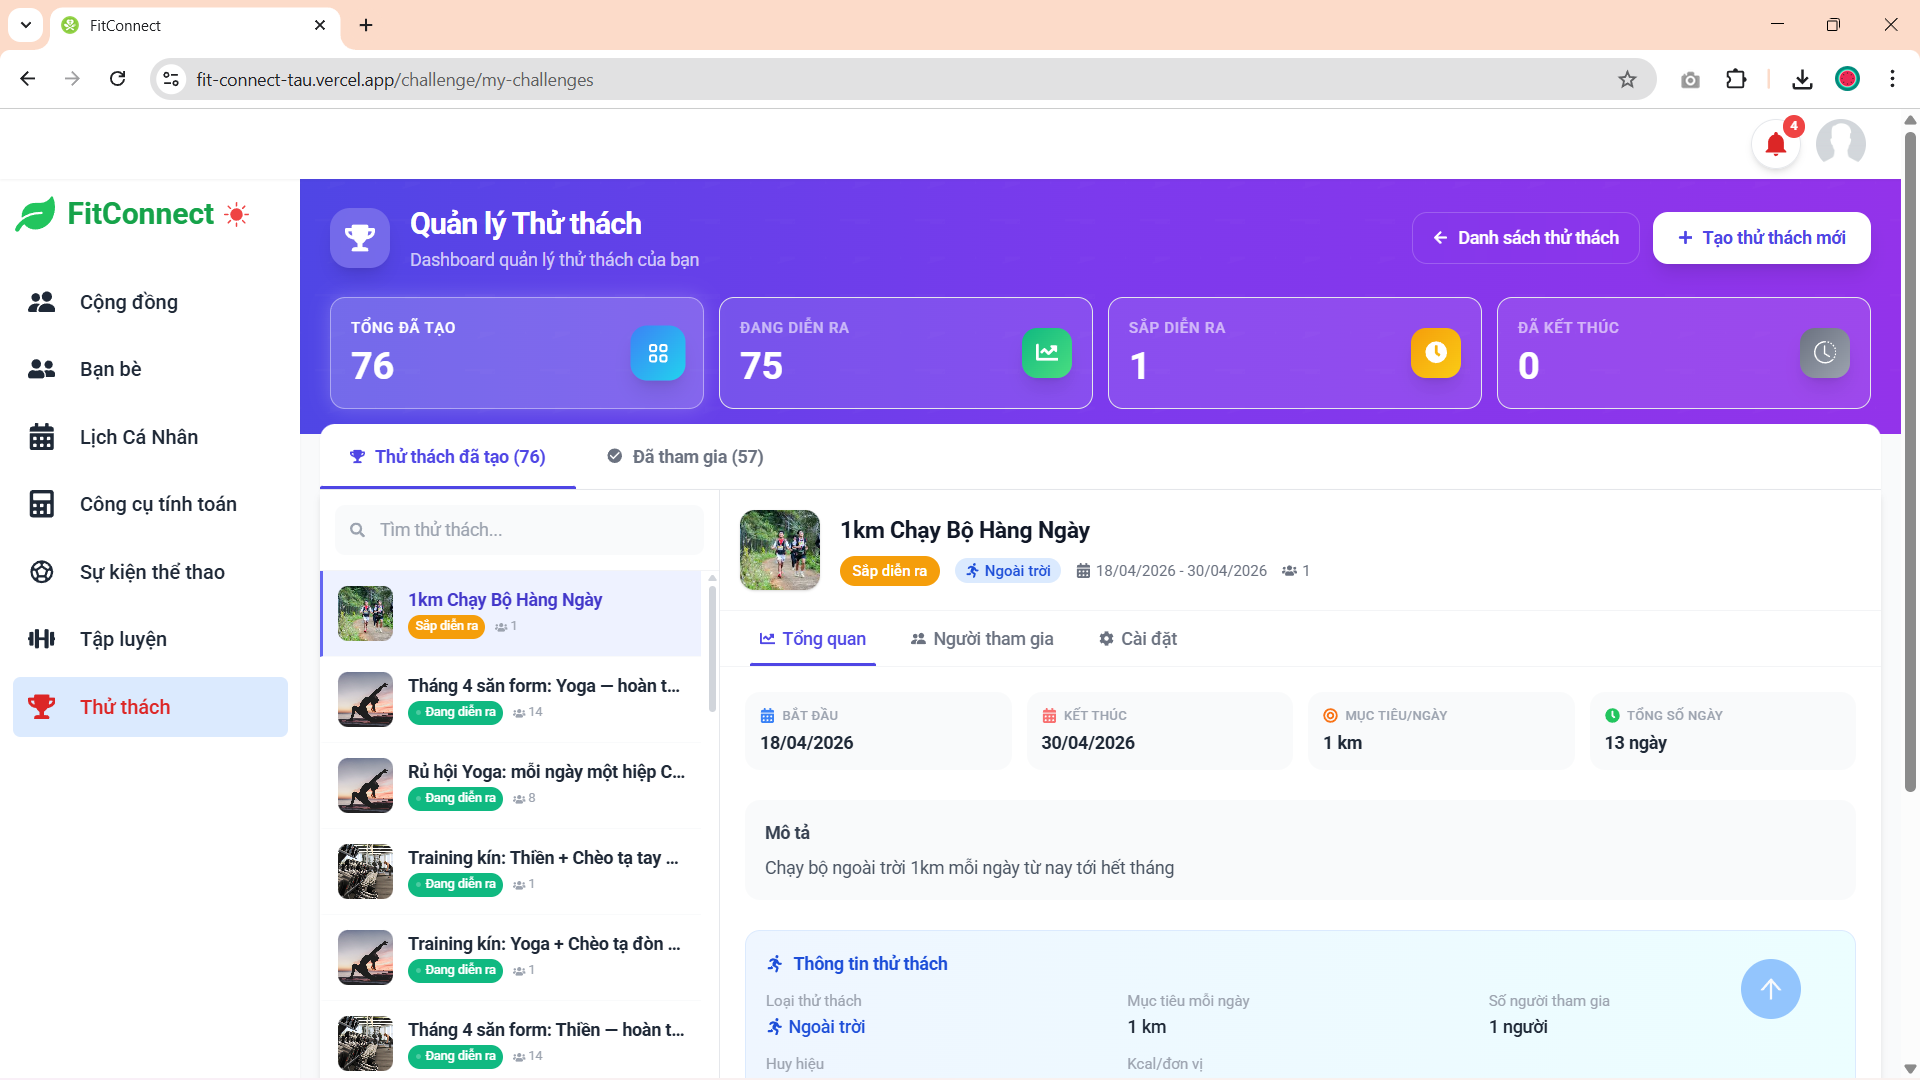
\includegraphics[width=\textwidth]{Images/IMG/nhom4/quanlythuthachvatongquanthu.png}
        \caption{Người dùng xem trang quản lý thử thách và tổng quan thử thách}
        \label{fig:impl_ch_manage}
    \end{subfigure}
    \hfill
    \begin{subfigure}[b]{0.30\textwidth}
        \centering
        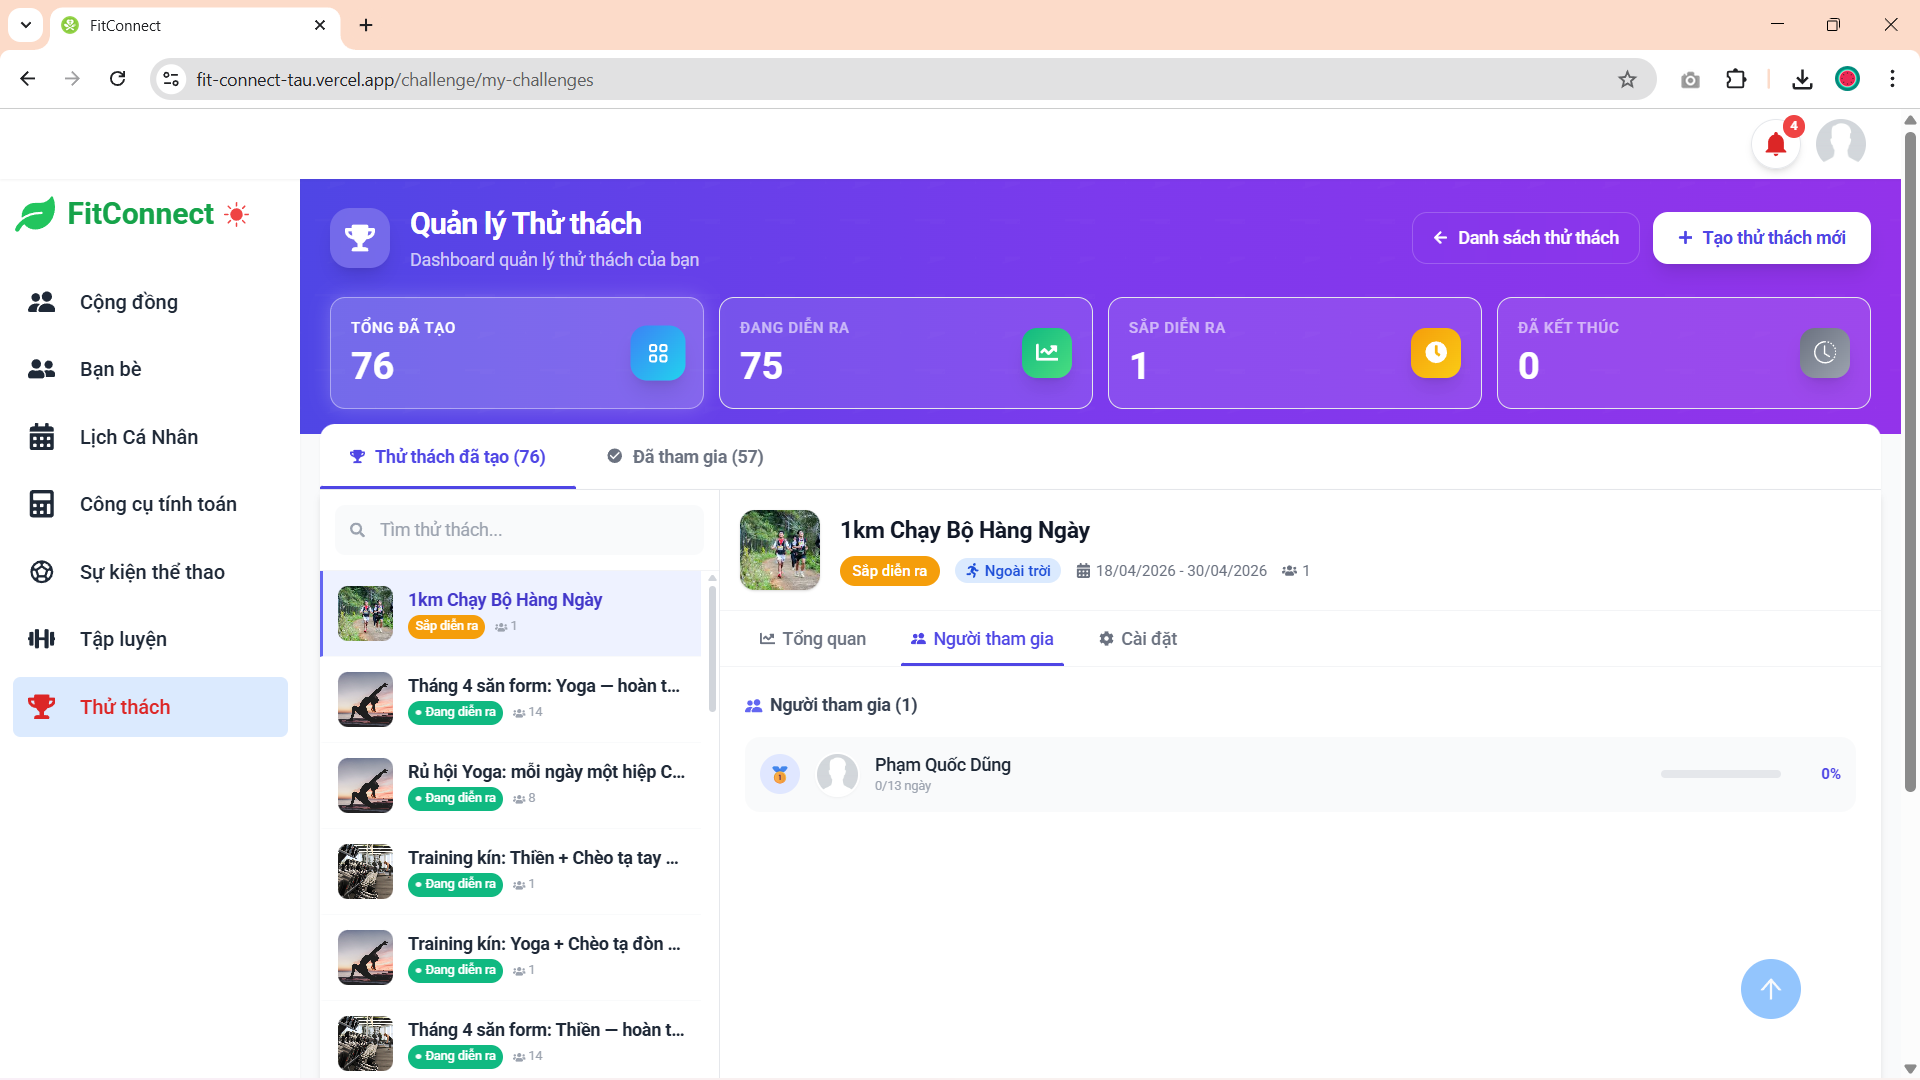
\includegraphics[width=\textwidth]{Images/IMG/nhom4/tabnguoithamgiathuthach.png}
        \caption{Người tạo xem tab Người tham gia thử thách}
        \label{fig:impl_ch_participants}
    \end{subfigure}
    \hfill
    \begin{subfigure}[b]{0.30\textwidth}
        \centering
        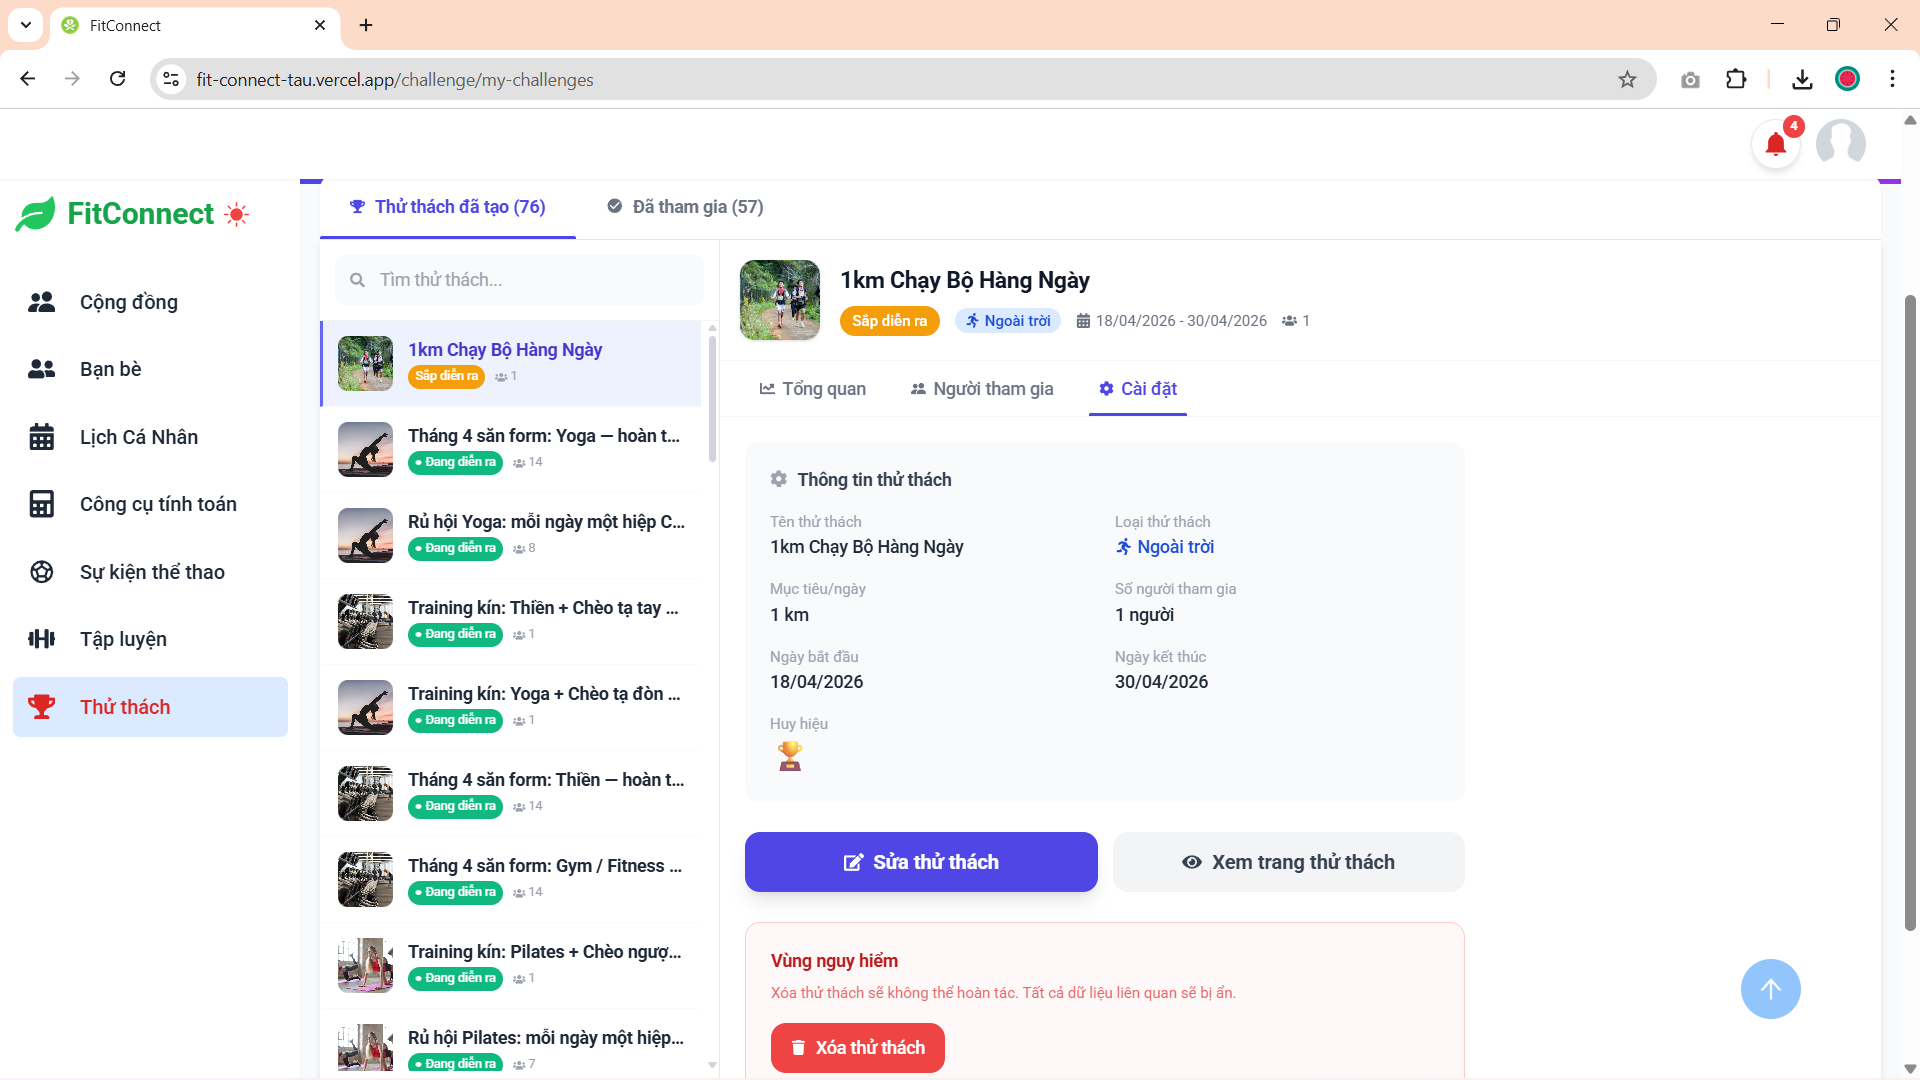
\includegraphics[width=\textwidth]{Images/IMG/nhom4/tabcaidatthuthach.png}
        \caption{Người tạo xem tab Cài đặt thử thách}
        \label{fig:impl_ch_settings}
    \end{subfigure}
\end{figure}


    \item Với chỉnh sửa thử thách: Người tạo có thể nhấn Sửa thử thách ở tab Cài đặt, hệ thống hiển thị modal chỉnh sửa với các thông tin tương tự khi tạo (lưu ý không thể thay đổi loại thử thách sau khi tạo). Sau khi chỉnh sửa, nhấn Lưu thay đổi để cập nhật.

\begin{figure}[H]
    \centering
    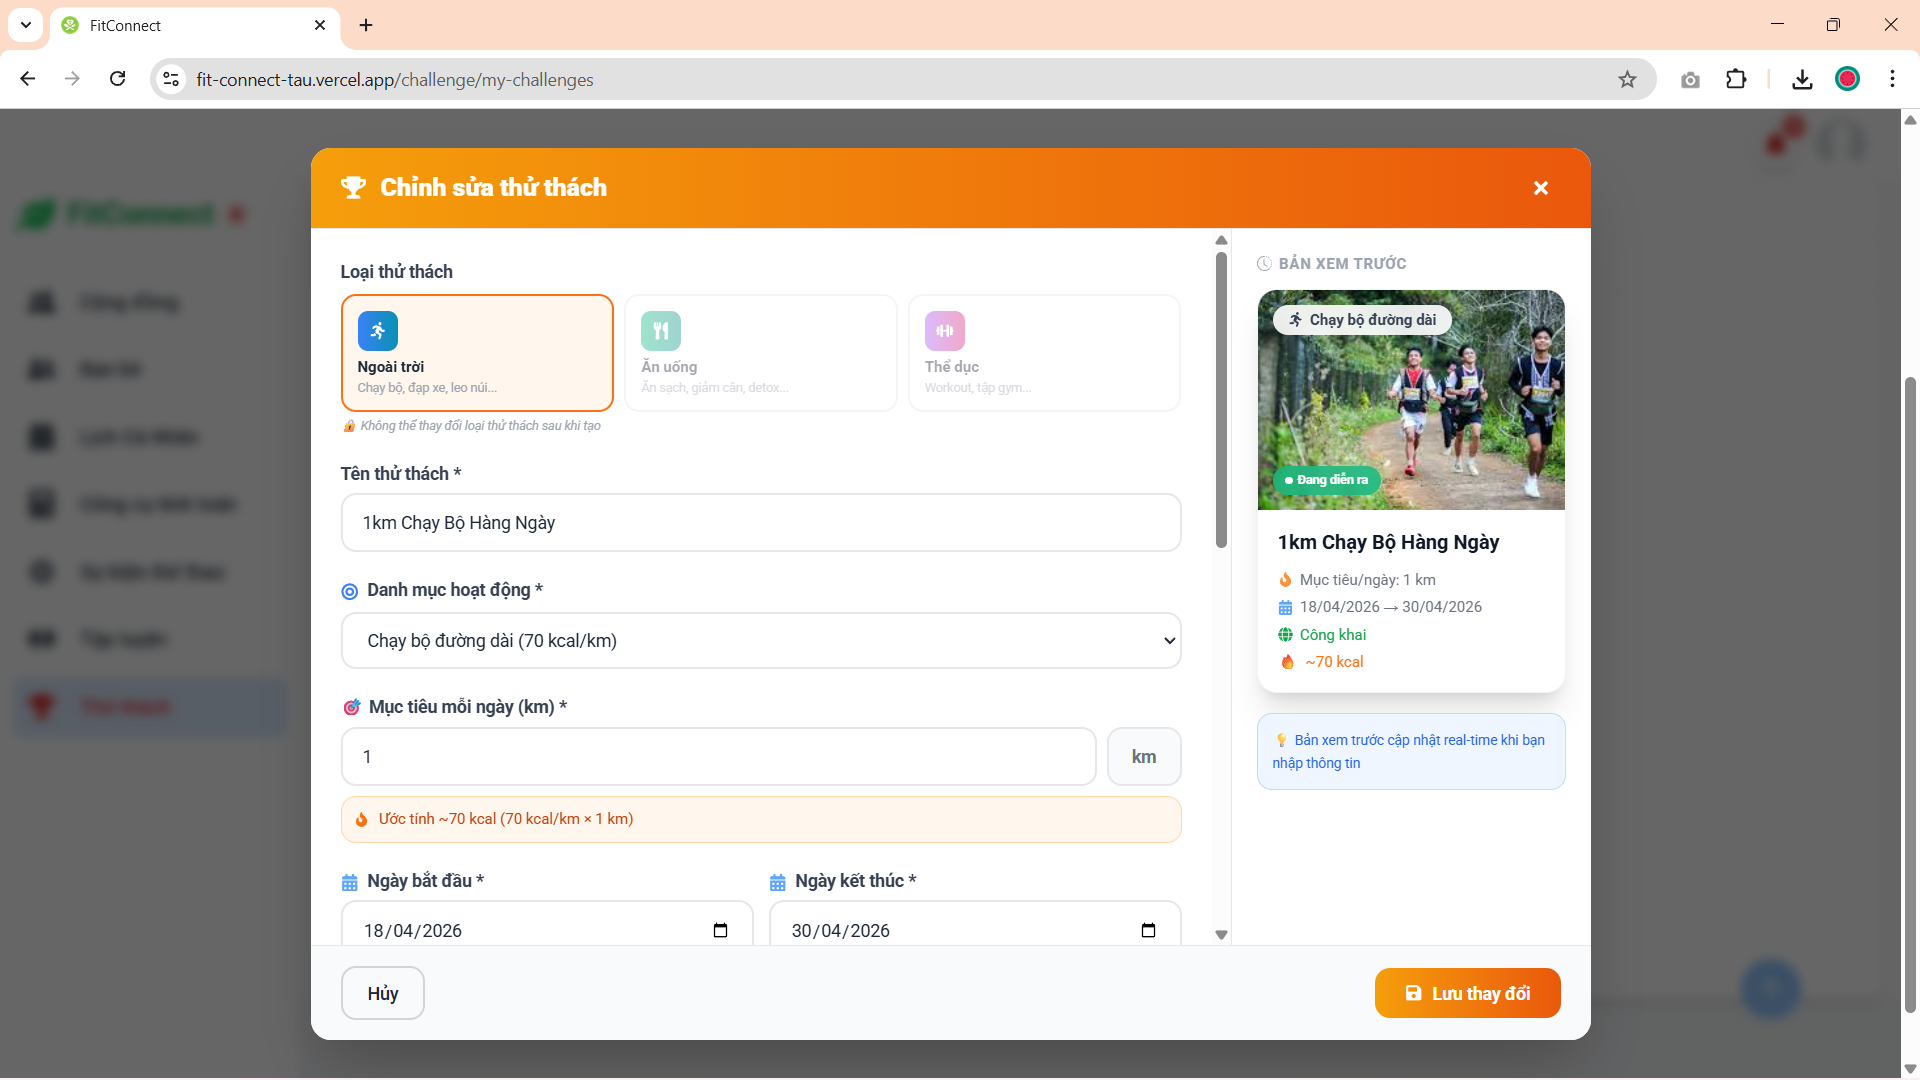
\includegraphics[width=0.60\textwidth]{Images/IMG/nhom4/chinhsuathuthach.png}
    \caption{Người tạo thao tác chỉnh sửa thử thách}
    \label{fig:impl_ch_edit}
\end{figure}

\end{itemize}

\subsubsection{Luồng thao tác tham gia thử thách (Góc độ Người tham gia)}
\begin{itemize}
    \item Với người dùng không phải người tạo, ở trang danh sách thử thách có thể lọc, tìm kiếm và tham gia thử thách. Khi nhấn vào thử thách, hệ thống hiển thị trang chi tiết thử thách với ba tab: Chi tiết, Tiến độ, và Người tham gia.

\begin{figure}[H]
    \centering
    \begin{subfigure}[b]{0.47\textwidth}
        \centering
        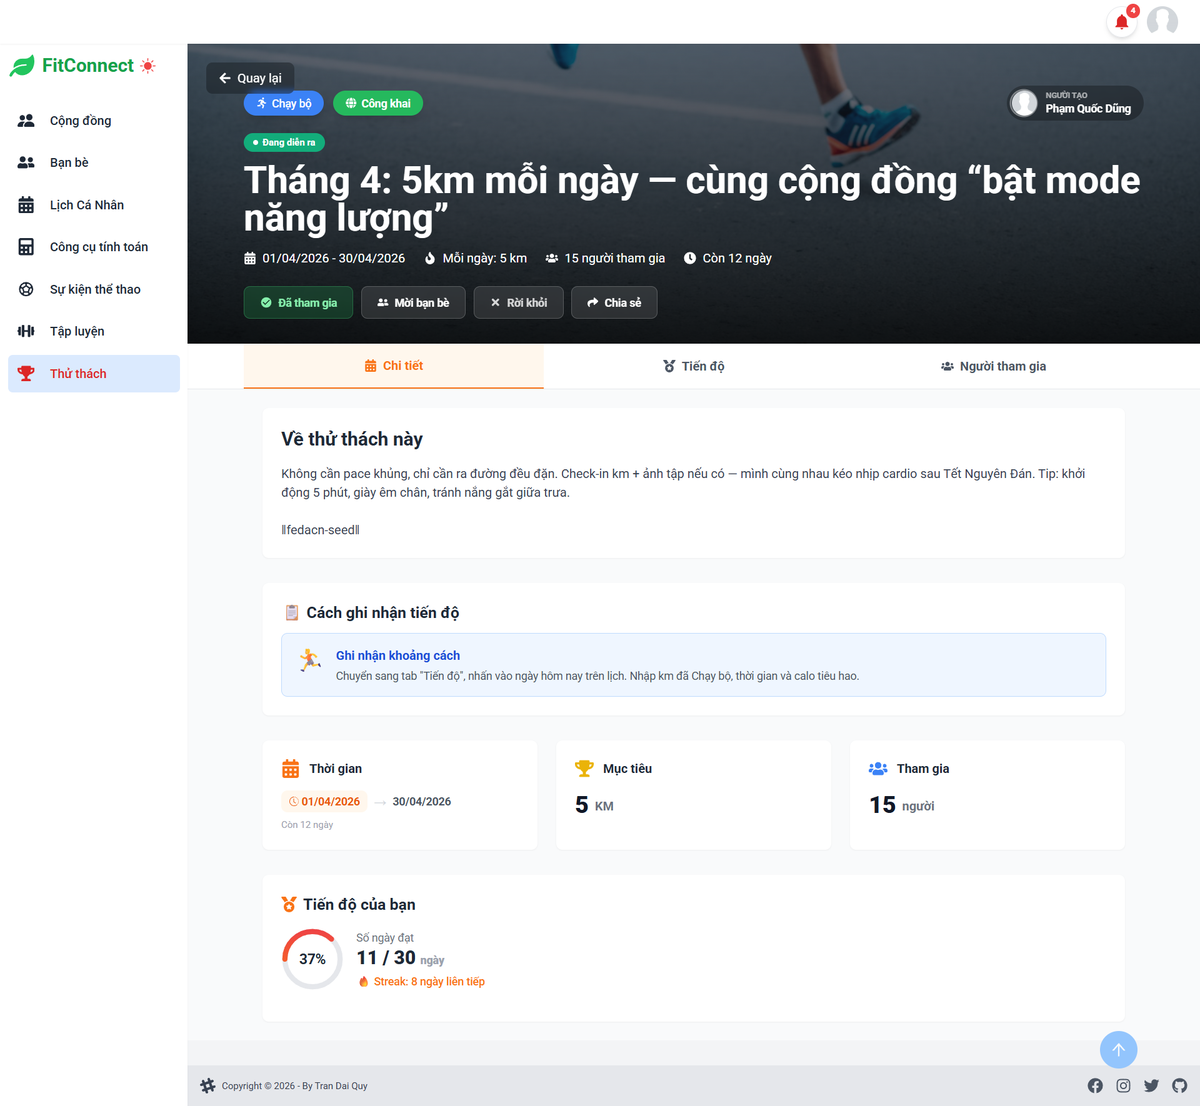
\includegraphics[width=\textwidth]{Images/IMG/nhom4/chitietthuthachdathamgia.png}
        \caption{Người tham gia xem chi tiết thử thách đã tham gia}
        \label{fig:impl_ch_detail}
    \end{subfigure}
    \hfill
    \begin{subfigure}[b]{0.47\textwidth}
        \centering
        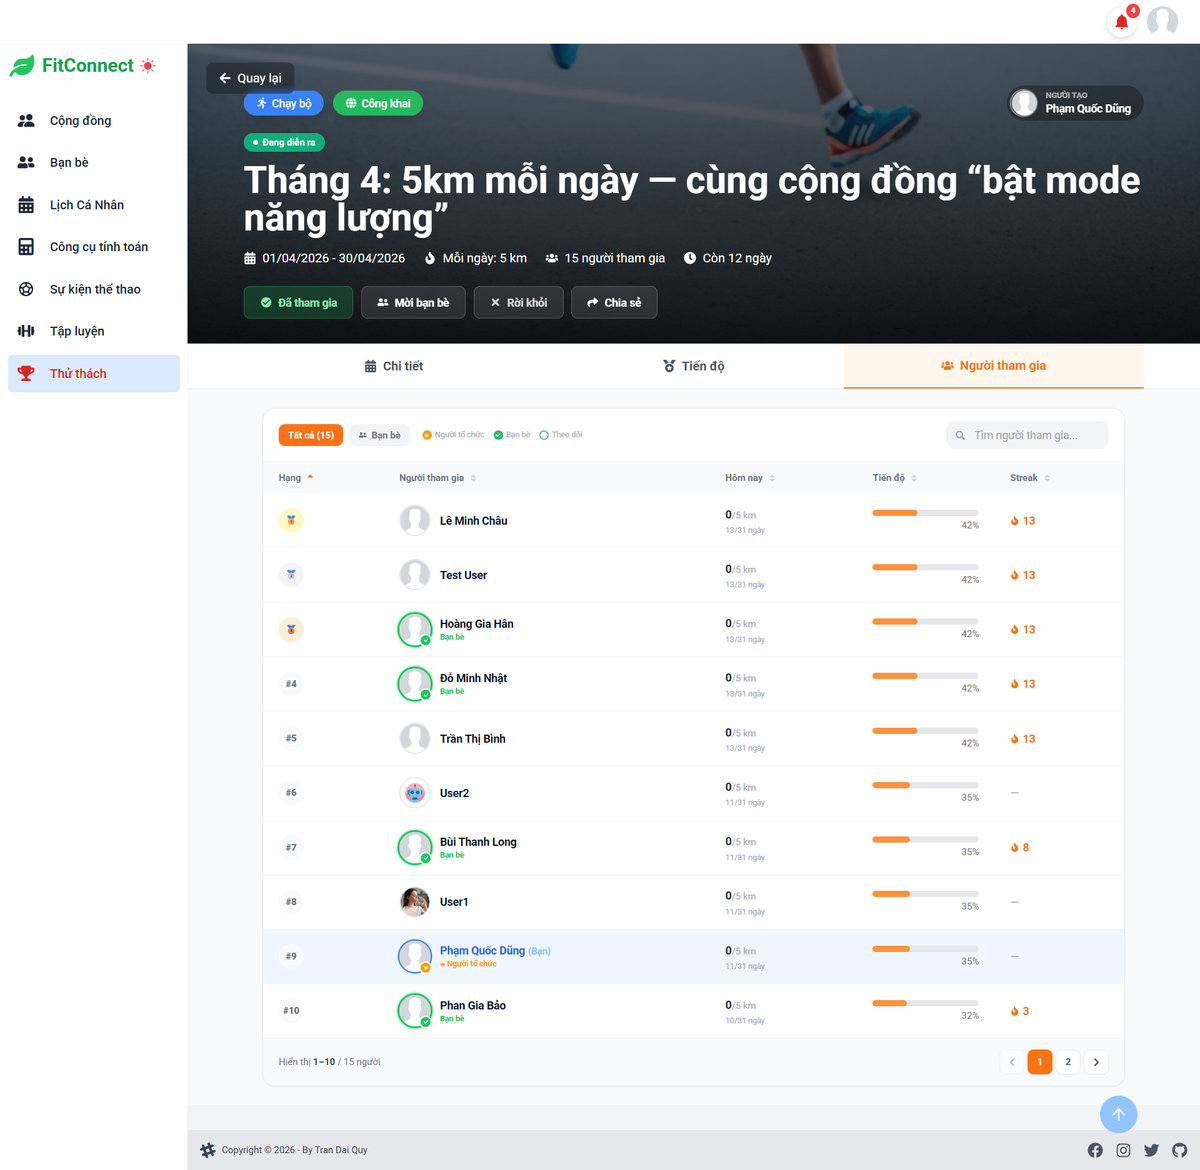
\includegraphics[width=\textwidth]{Images/IMG/nhom4/danhsachnguoithamgiathuthach.png}
        \caption{Người tham gia xem danh sách người tham gia thử thách}
        \label{fig:impl_ch_member_list}
    \end{subfigure}
\end{figure}


    \item Người tham gia có thể xem tab Tiến độ để theo dõi quá trình hoàn thành thử thách. Hệ thống hiển thị: số ngày hoàn thành, tổng số ngày, tỷ lệ hoàn thành, thanh tiến độ tổng thể, và lịch theo tháng hiển thị chi tiết trạng thái từng ngày (Hoàn thành, Đang diễn ra, Đã kết thúc, Chưa diễn ra) kèm quãng đường/số bữa đã ghi nhận.

\begin{figure}[H]
    \centering
    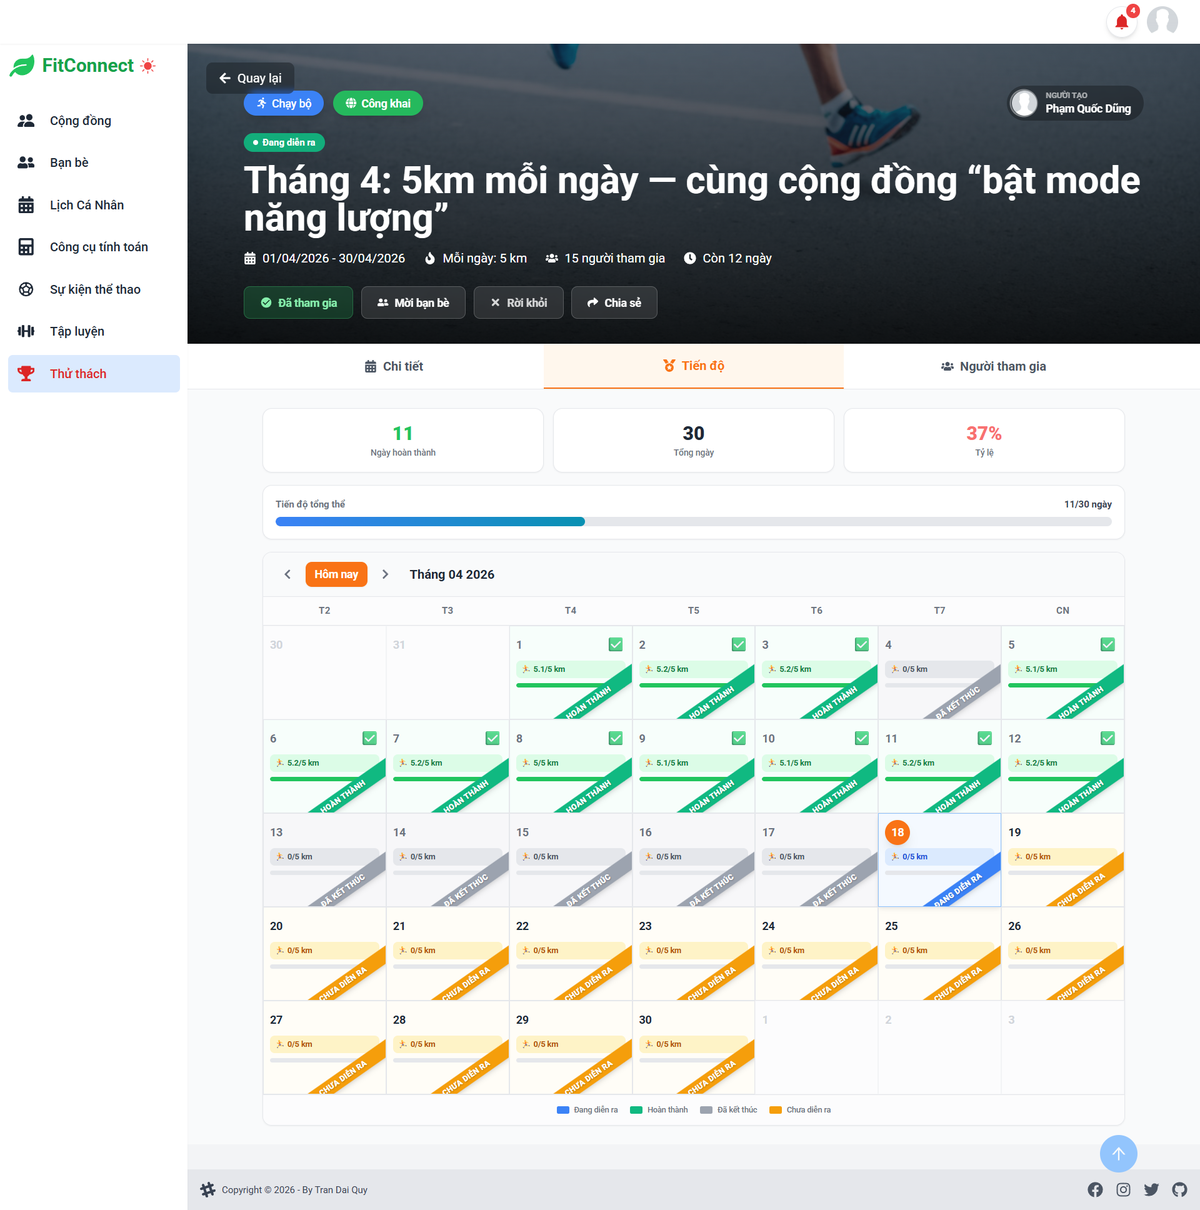
\includegraphics[width=0.60\textwidth]{Images/IMG/nhom4/tabtiendothuthach.png}
    \caption{Người tham gia xem tab Tiến độ thử thách theo lịch}
    \label{fig:impl_ch_progress}
\end{figure}


    \item Tại tab Tiến độ hoặc khi xem chi tiết hoạt động của người tham gia khác, người dùng có thể tương tác bằng cách gửi bình luận. Hệ thống hiển thị phần bình luận bên dưới chi tiết hoạt động (ví dụ: ngày ghi nhận, số km/bữa ăn), cho phép người tham gia nhập thông điệp động viên và trao đổi với các thành viên khác.

\begin{figure}[H]
    \centering
    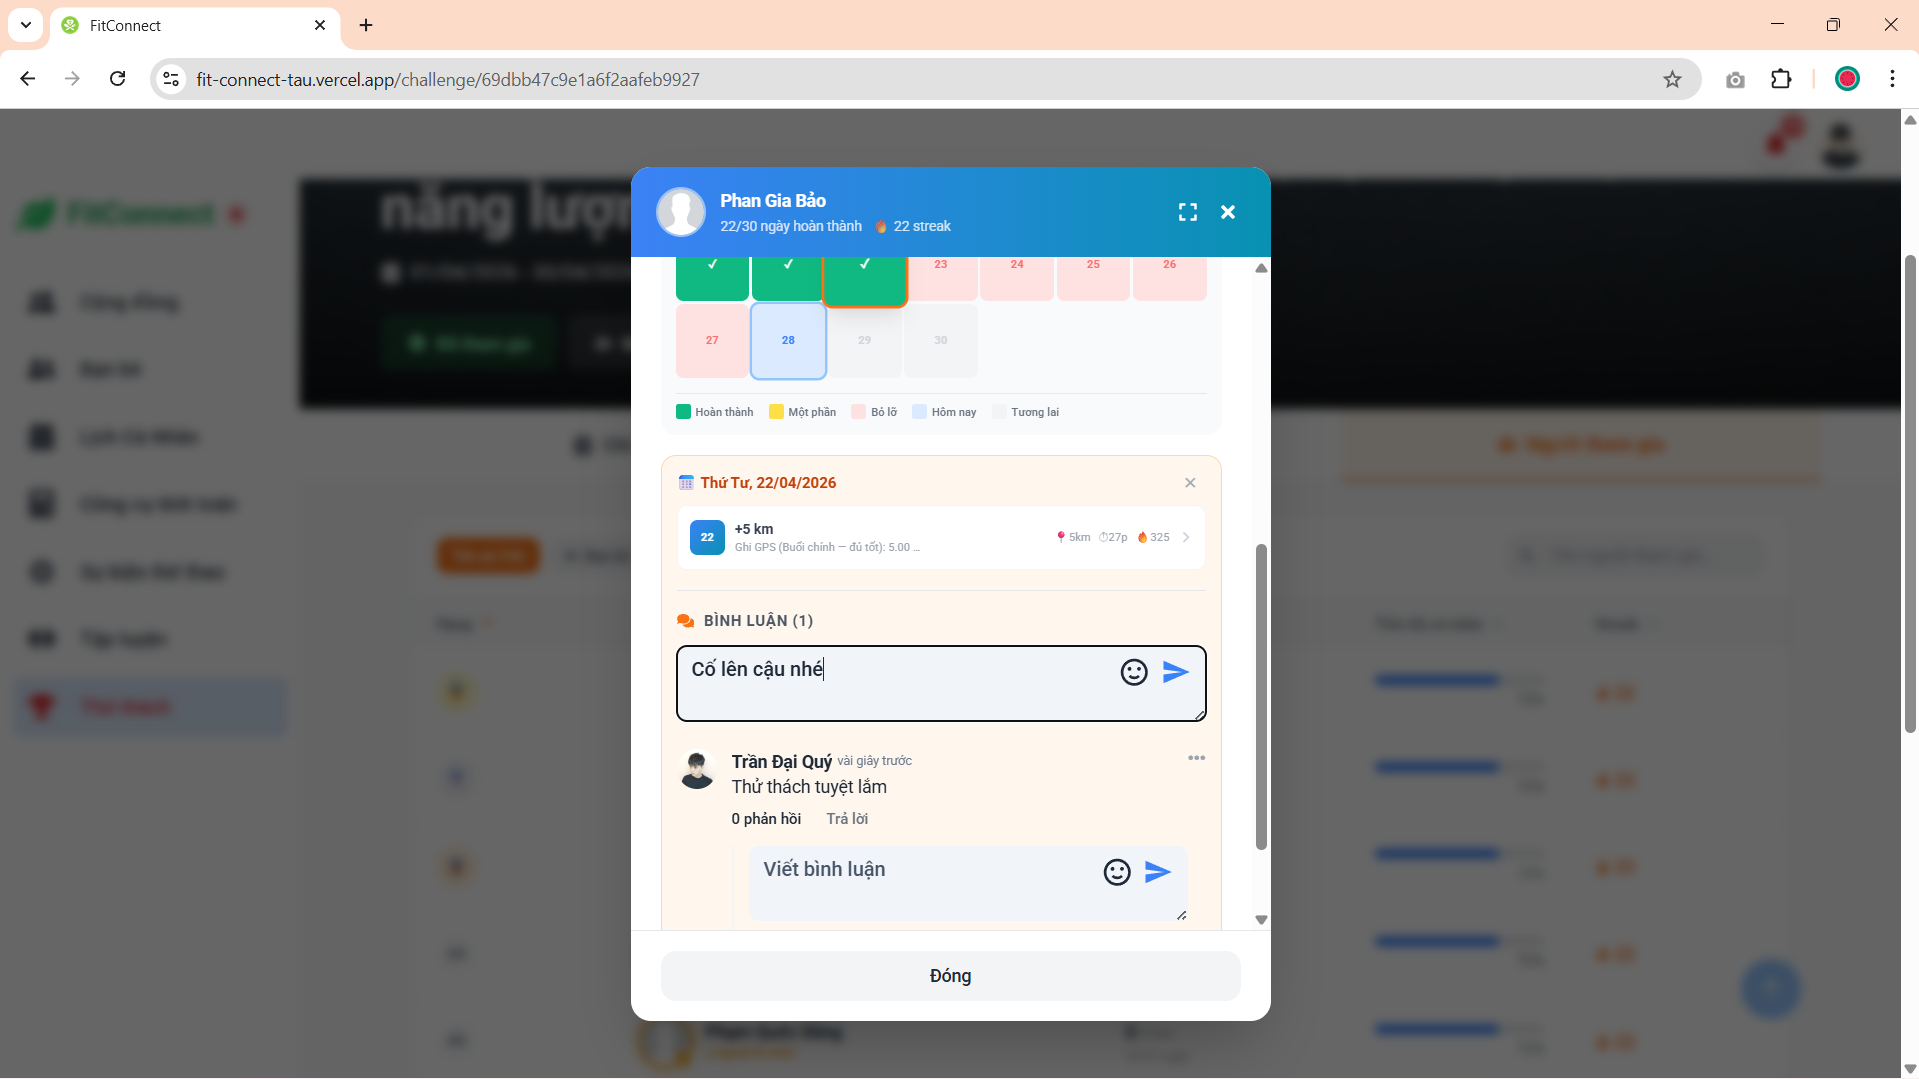
\includegraphics[width=0.60\textwidth]{Images/IMG/nhom4/binhluanthuthachnguoithamgia.png}
    \caption{Người tham gia bình luận vào hoạt động thử thách của thành viên khác}
    \label{fig:impl_ch_comment}
\end{figure}


    \item Người tham gia có thể chia sẻ thử thách lên trang Cộng đồng; bài viết thử thách sẽ tự động xuất hiện trên Bảng tin cộng đồng.

\begin{figure}[H]
    \centering
    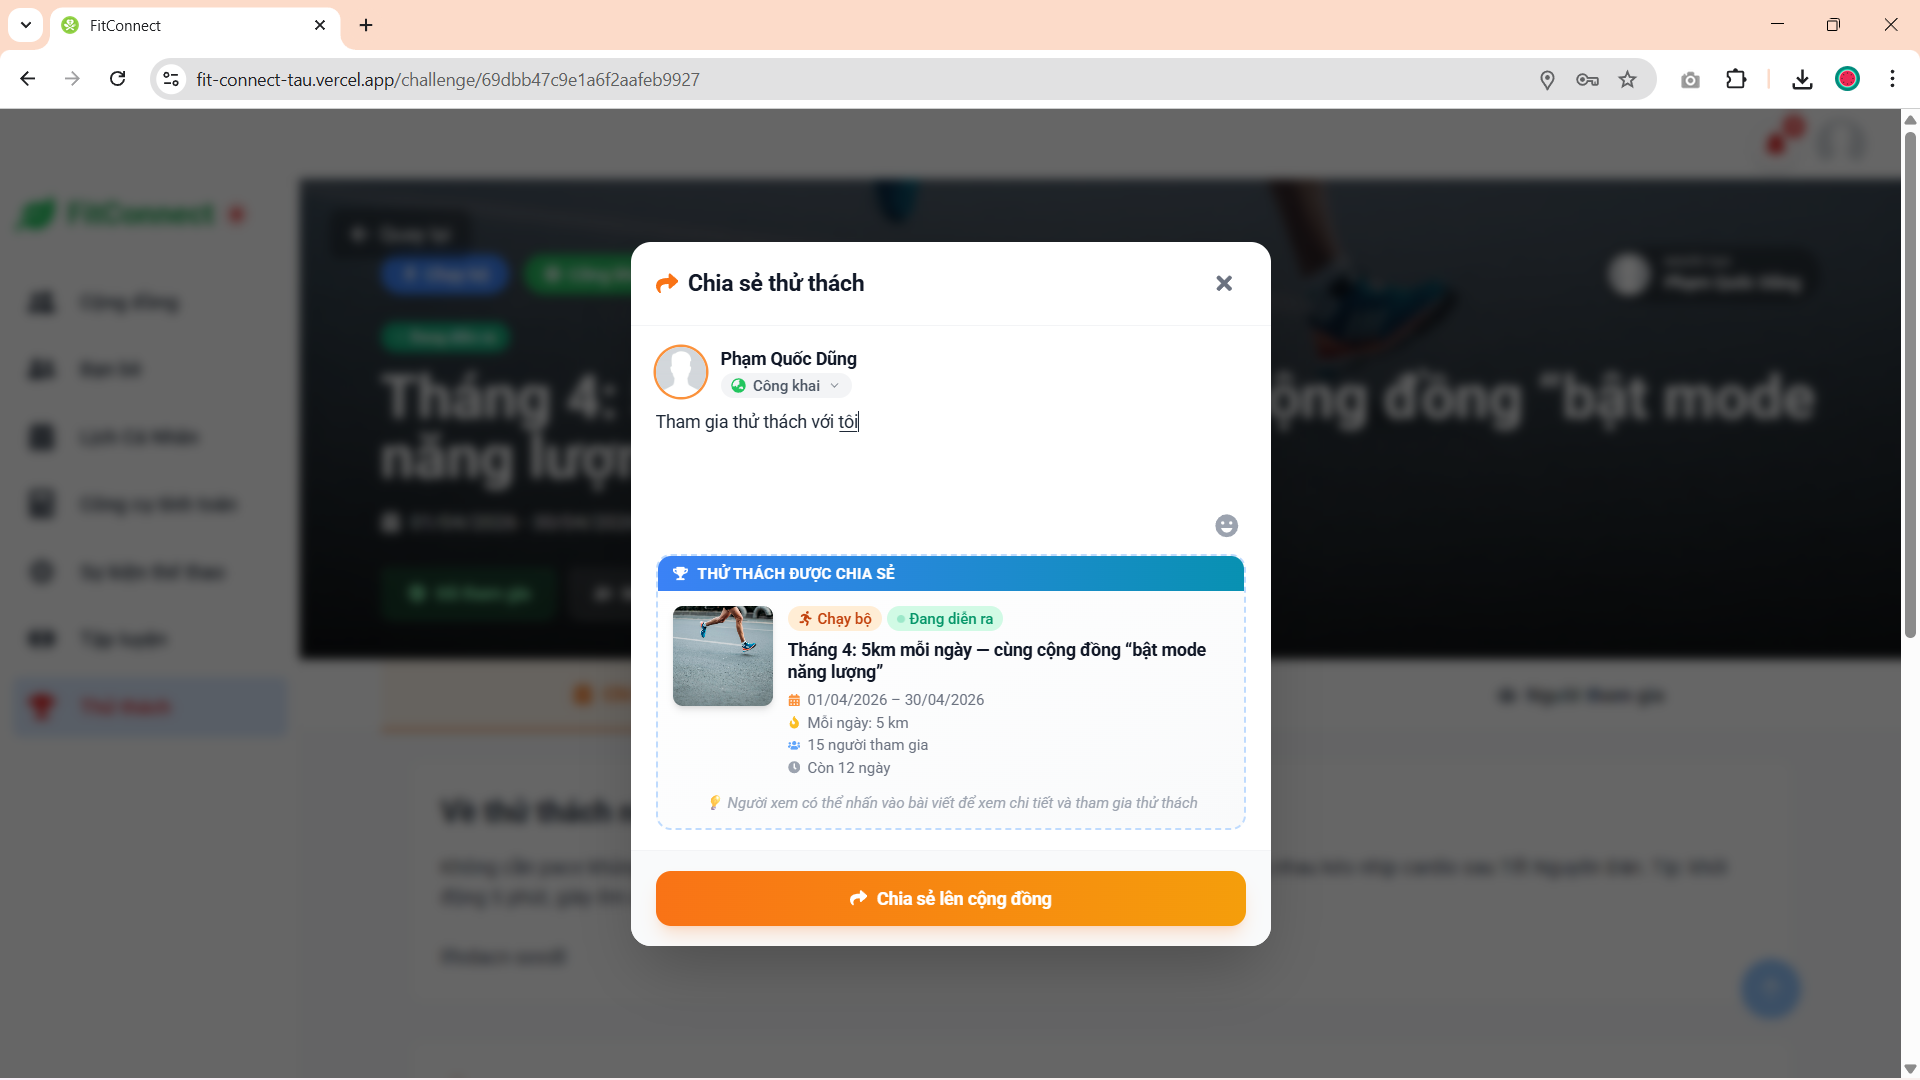
\includegraphics[width=0.60\textwidth]{Images/IMG/nhom4/chiasethuthach.png}
    \caption{Người tham gia thao tác chia sẻ thử thách lên cộng đồng}
    \label{fig:impl_ch_share}
\end{figure}


    \item Người tham gia có thể mời bạn bè tham gia thử thách. Hệ thống hiển thị modal tìm kiếm và mời bạn bè, bạn bè được mời sẽ nhận được thông báo.

\begin{figure}[H]
    \centering
    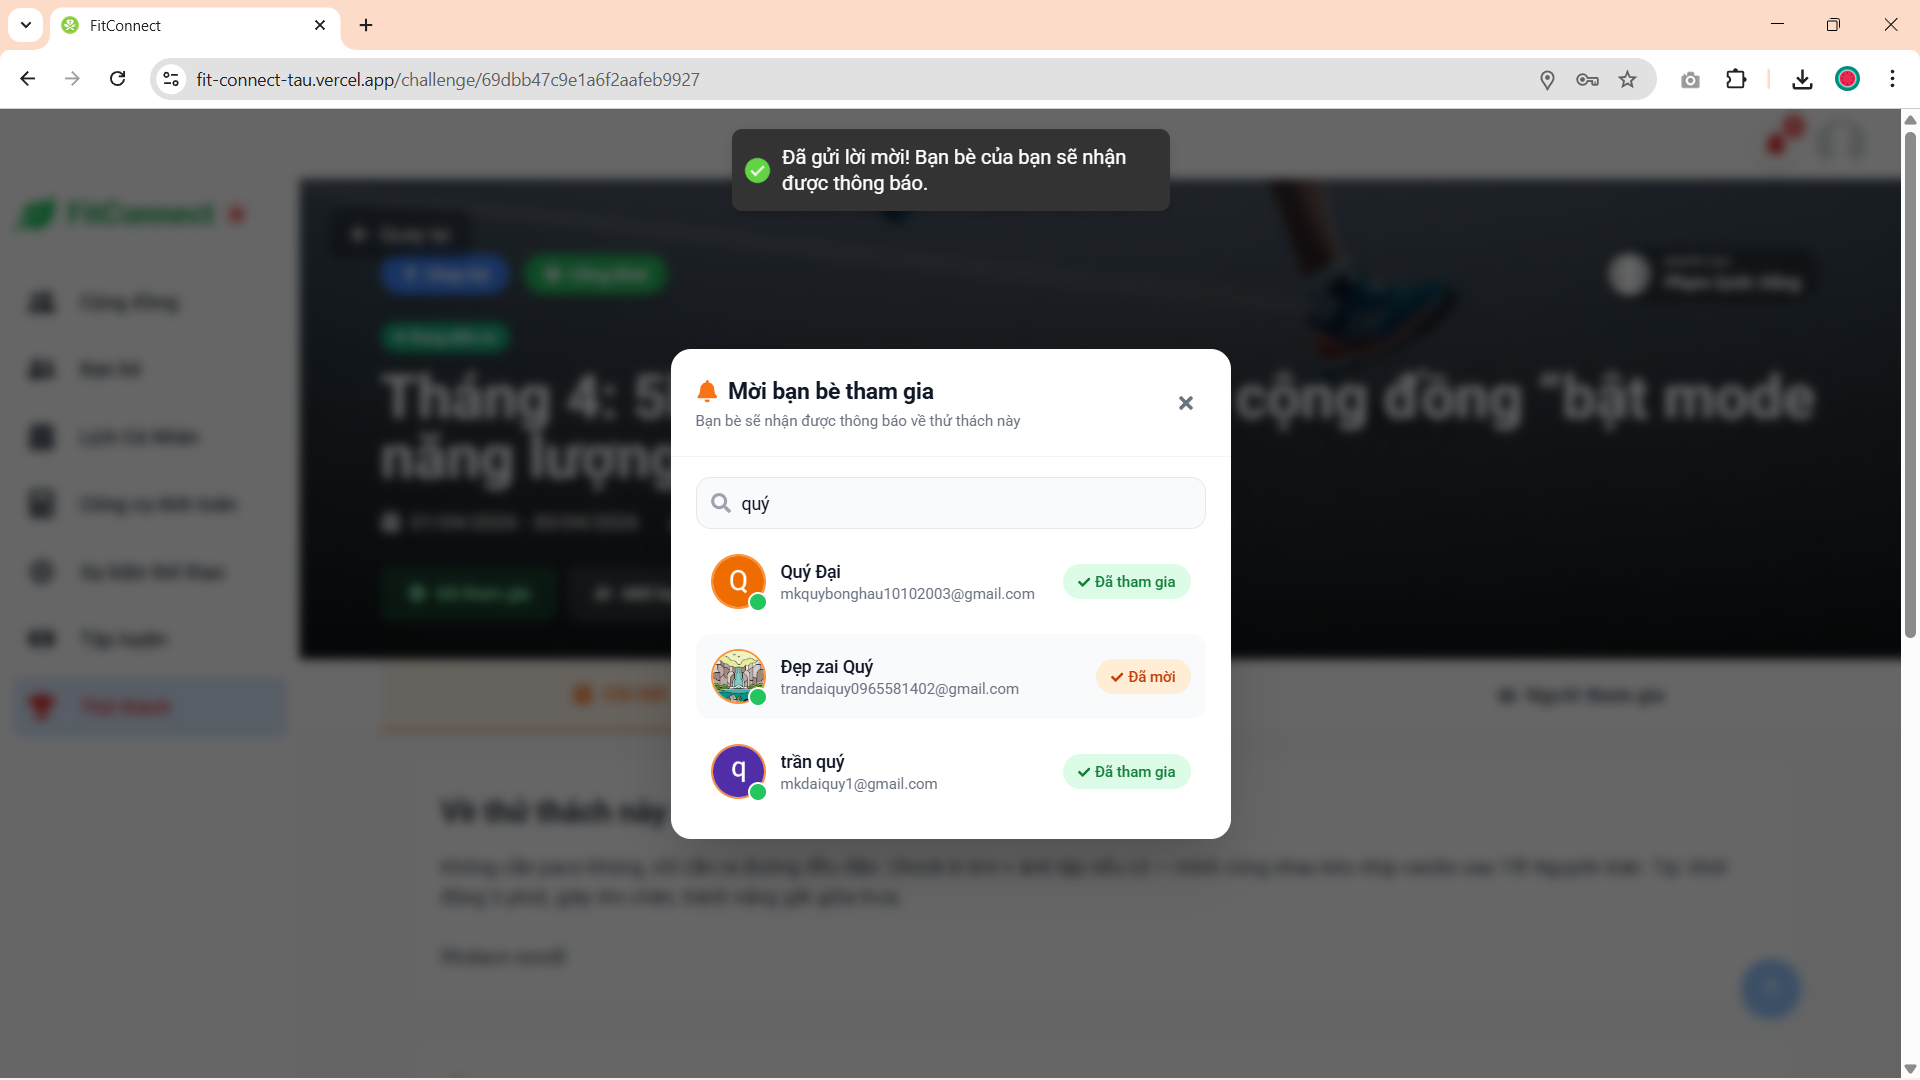
\includegraphics[width=0.60\textwidth]{Images/IMG/nhom4/moibanbethamgiathuthach.png}
    \caption{Người tham gia thao tác mời bạn bè tham gia thử thách}
    \label{fig:impl_ch_invite}
\end{figure}


    \item Người tham gia có thể báo cáo thử thách vi phạm lên Quản trị viên bằng cách nhập lý do báo cáo và nhấn Gửi báo cáo.

\begin{figure}[H]
    \centering
    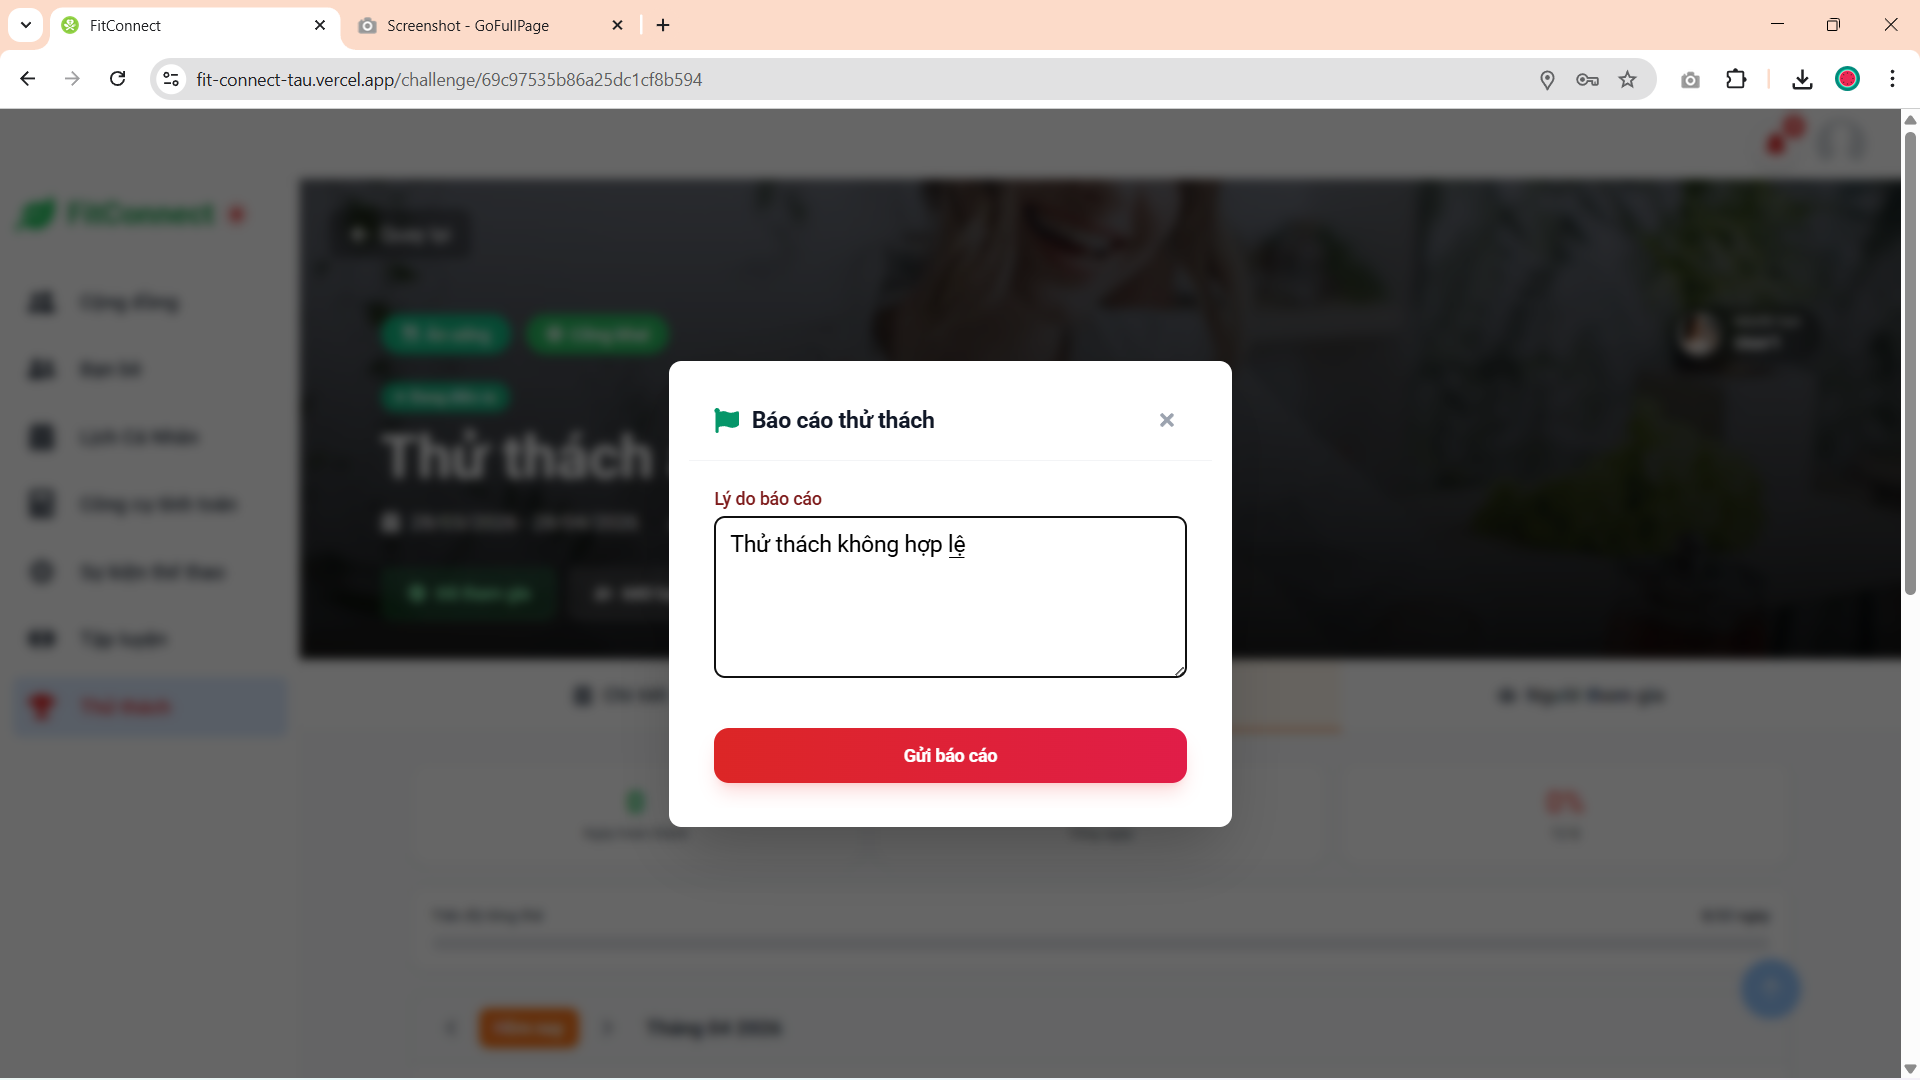
\includegraphics[width=0.60\textwidth]{Images/IMG/nhom4/baocaothuthach.png}
    \caption{Người tham gia thao tác báo cáo thử thách}
    \label{fig:impl_ch_report}
\end{figure}

\end{itemize}

\textbf{Ghi nhận tiến độ thử thách hàng ngày:}

\textbf{a) Đối với thử thách Ngoài trời (chạy bộ, đạp xe,...):}
\begin{itemize}
    \item Người tham gia nhấn vào ngày hiện tại trên lịch tiến độ, hệ thống hiển thị modal bắt đầu ghi với thông tin mục tiêu ngày (km) và nút Bắt đầu ghi. Khi nhấn Bắt đầu ghi, hệ thống chuyển sang trang GPS Tracking hiển thị bản đồ với vị trí hiện tại, quãng đường (km), thời gian, tốc độ (km/h), calories (kcal) và thanh tiến độ mục tiêu ngày.

\begin{figure}[H]
    \centering
    \begin{subfigure}[b]{0.47\textwidth}
        \centering
        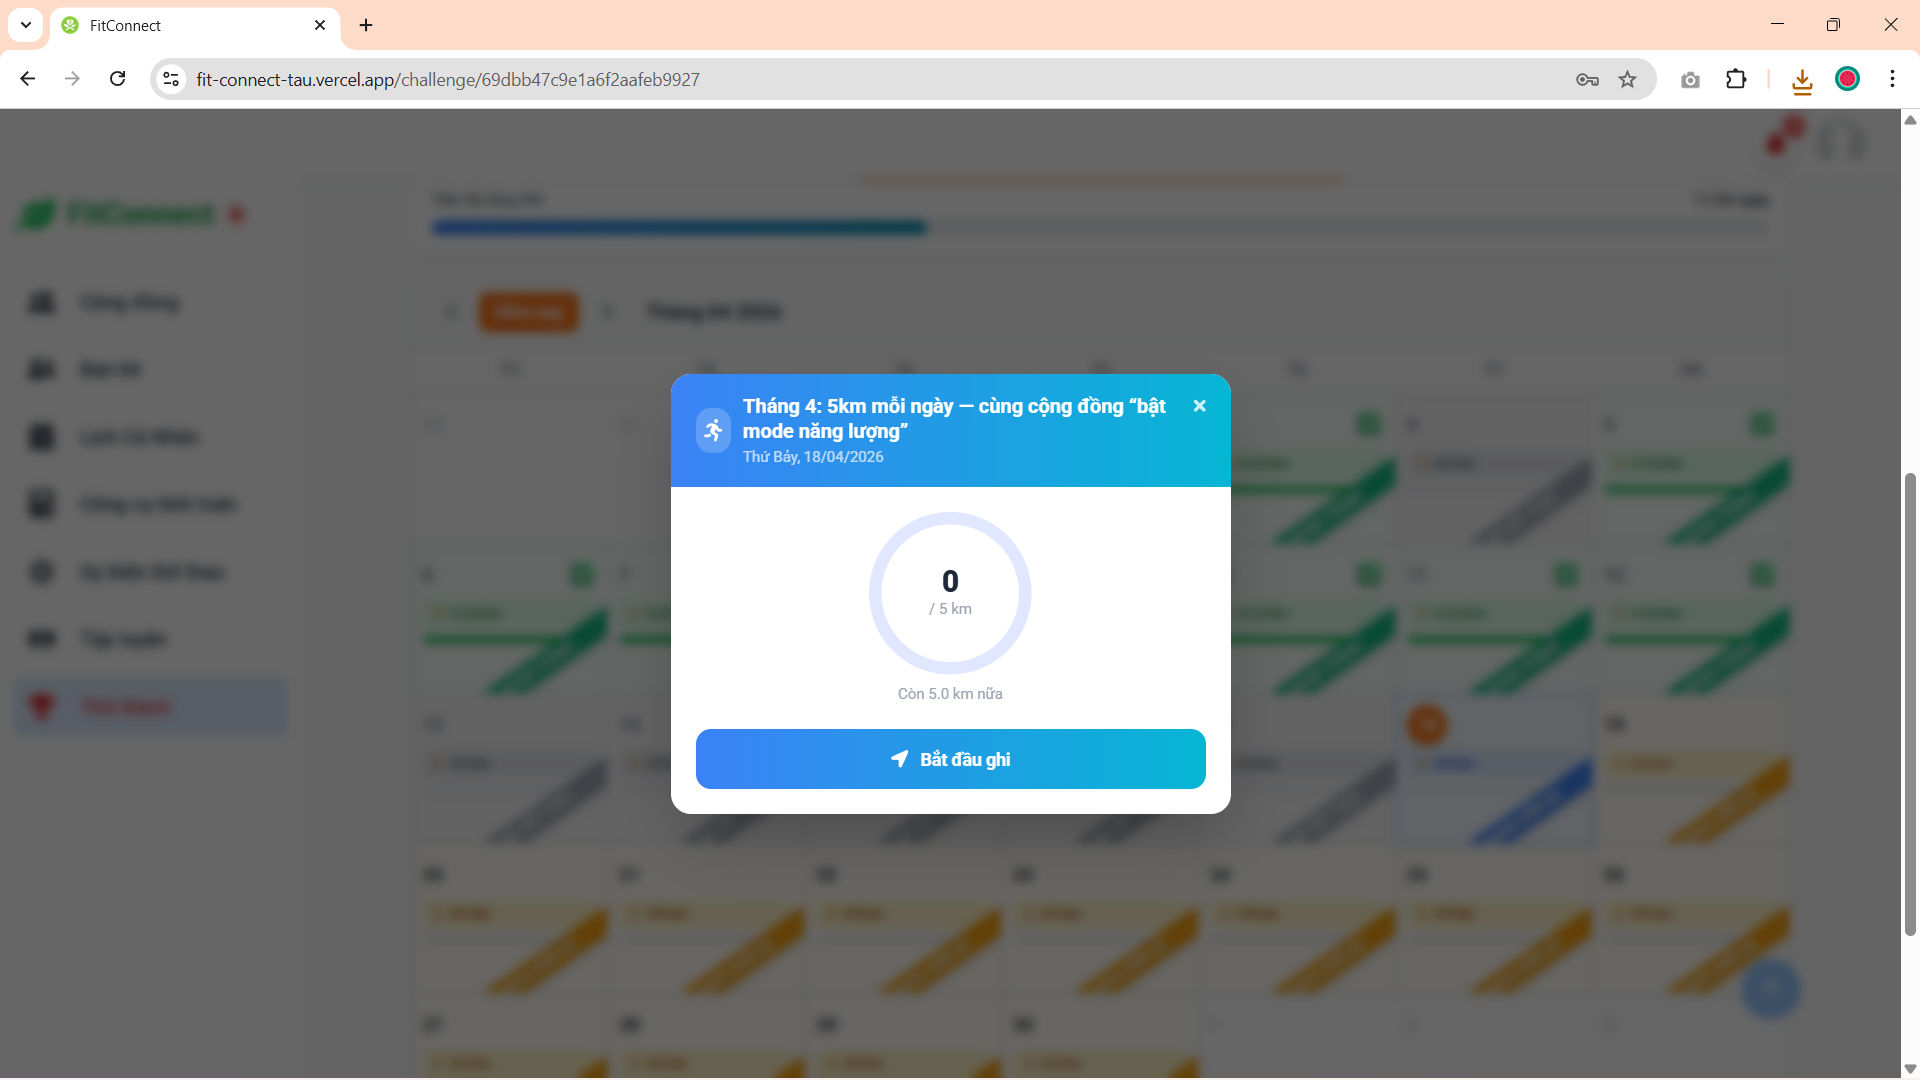
\includegraphics[width=\textwidth]{Images/IMG/nhom4/manhinhbatdauthuchienttchaybo.png}
        \caption{Hệ thống hiển thị modal bắt đầu thực hiện thử thách chạy bộ}
        \label{fig:impl_ch_start_run}
    \end{subfigure}
    \hfill
    \begin{subfigure}[b]{0.47\textwidth}
        \centering
        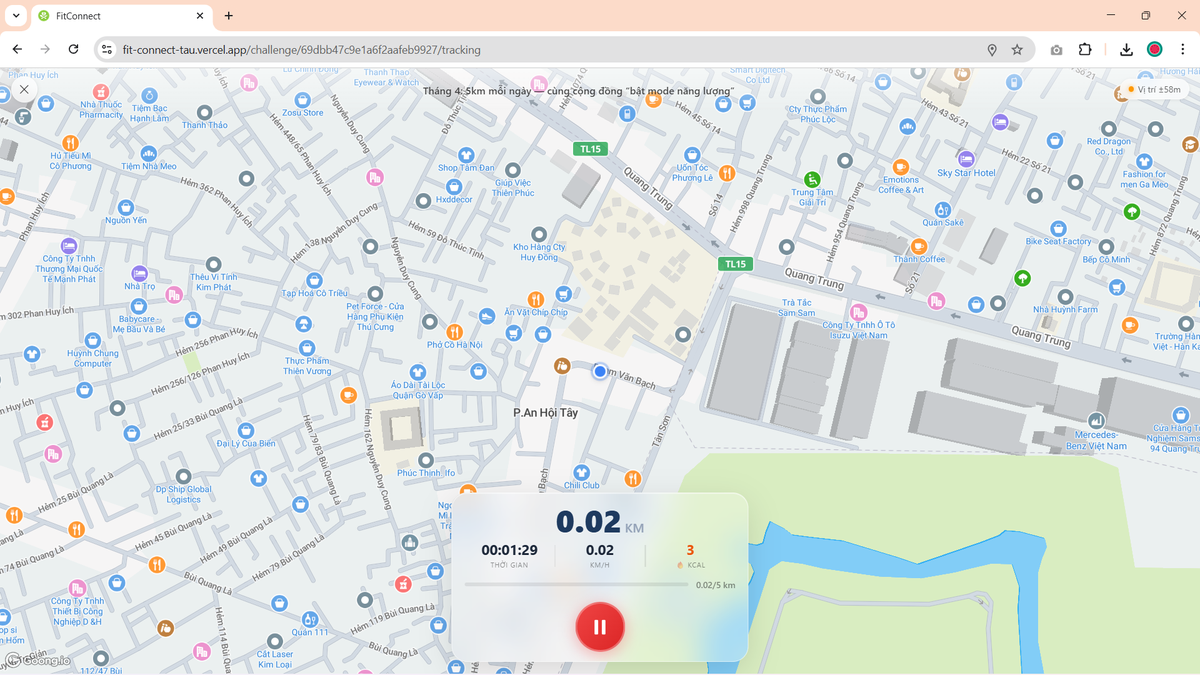
\includegraphics[width=\textwidth]{Images/IMG/nhom4/giaodienthuthachchaybo.png}
        \caption{Người tham gia ghi tiến độ thử thách chạy bộ bằng GPS tracking}
        \label{fig:impl_ch_gps}
    \end{subfigure}
\end{figure}


    \item Khi nhấn hoàn thành, hệ thống tổng hợp và hiển thị kết quả: quãng đường (km), thời gian, calories (kcal), vận tốc trung bình. Người tham gia nhấn Xác nhận để lưu kết quả vào tiến độ thử thách.

\end{itemize}

\textbf{b) Đối với thử thách Ăn uống (ăn sạch, giảm cân, detox,...):}
\begin{itemize}
    \item Người tham gia nhấn vào ngày hiện tại trên lịch tiến độ, hệ thống hiển thị modal bắt đầu ghi tiến độ bữa ăn với thông tin mục tiêu ngày (số bữa), danh sách các lần hoạt động đã ghi nhận và nút Bắt đầu thực hiện.

\begin{figure}[H]
    \centering
    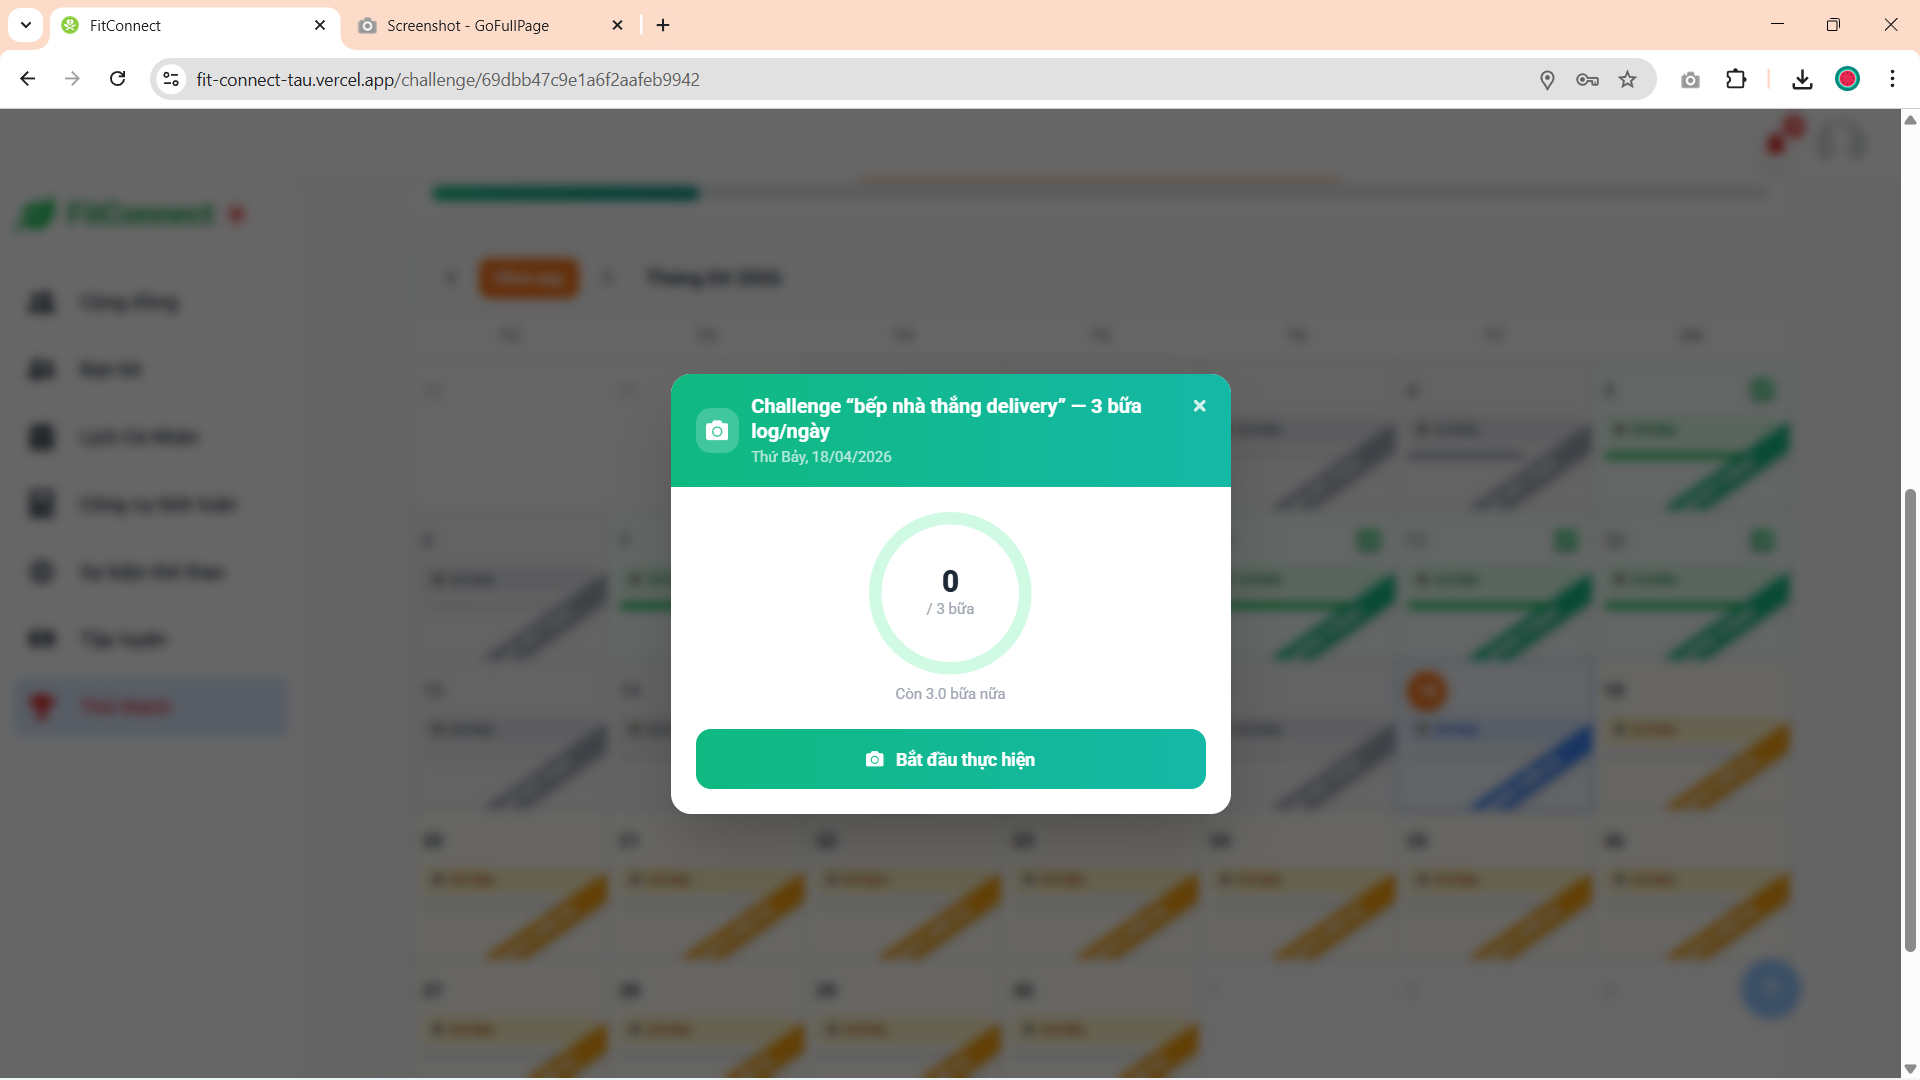
\includegraphics[width=0.60\textwidth]{Images/IMG/nhom4/1modalbatdaughitiendobuaan.png}
    \caption{Hệ thống hiển thị modal bắt đầu ghi tiến độ bữa ăn}
    \label{fig:impl_ch_food_start}
\end{figure}


    \item Khi nhấn Bắt đầu thực hiện, hệ thống hiển thị modal Ghi nhận bữa ăn với các thông tin: loại bữa ăn (Bữa sáng, Bữa trưa, Bữa tối, Bữa phụ), tên món ăn, ảnh bữa ăn (bắt buộc để Check-in, AI sẽ tự động xác minh ảnh), kcal ước tính (tùy chọn), và mô tả.

\begin{figure}[H]
    \centering
    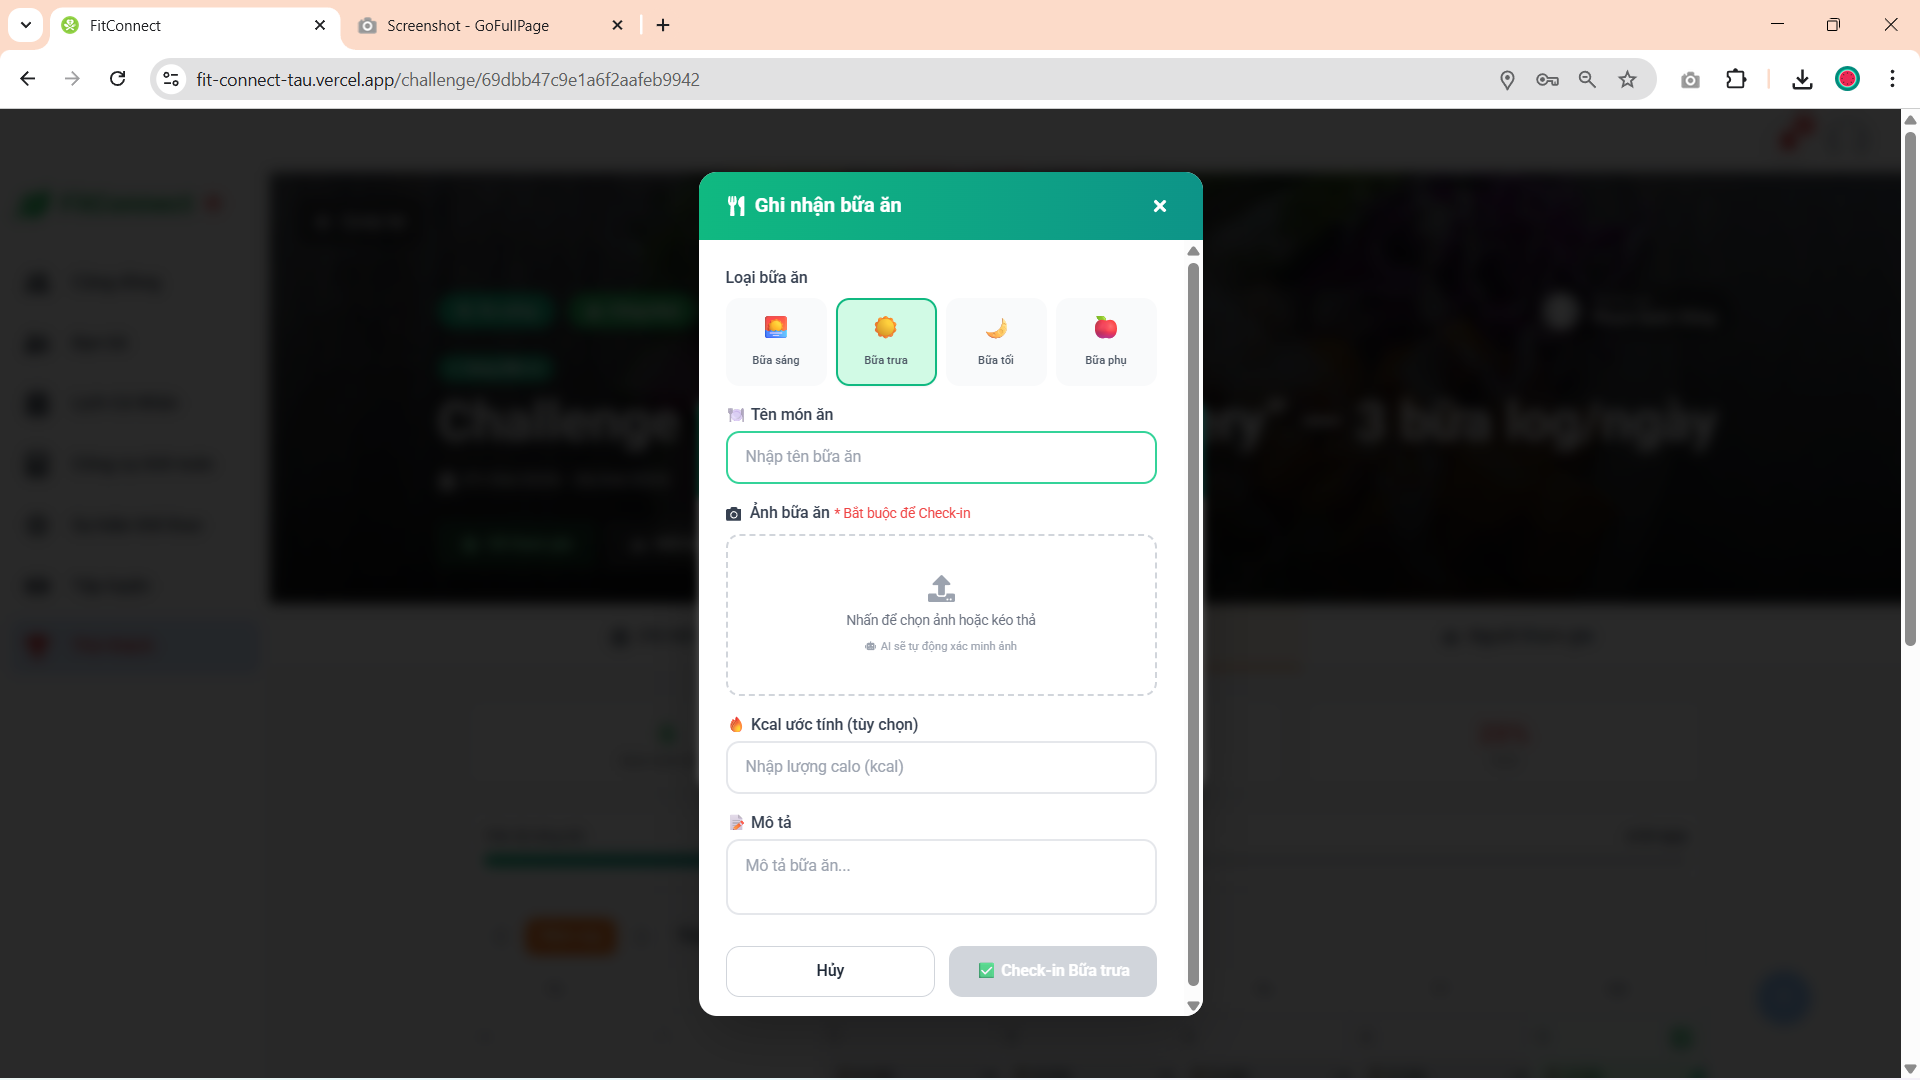
\includegraphics[width=0.60\textwidth]{Images/IMG/nhom4/1modalcheckingbuaan.png}
    \caption{Hệ thống hiển thị modal ghi nhận bữa ăn}
    \label{fig:impl_ch_food_form}
\end{figure}


    \item Sau khi tải ảnh bữa ăn lên, hệ thống sử dụng AI tự động xác minh ảnh. Nếu ảnh hợp lệ, hệ thống hiển thị thông báo ``Ảnh hợp lệ'' kèm nhận xét của AI về ảnh, và cho phép Check-in bữa ăn.

\begin{figure}[H]
    \centering
    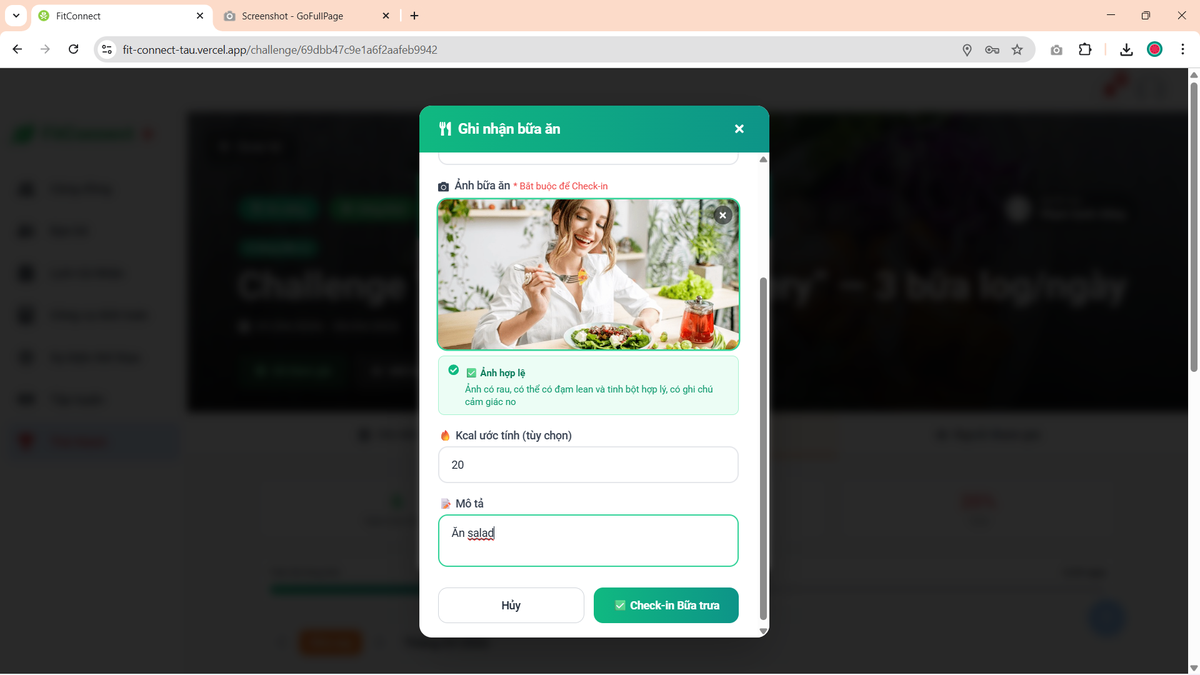
\includegraphics[width=0.60\textwidth]{Images/IMG/nhom4/1checkingbuaanhople.png}
    \caption{Hệ thống AI xác minh ảnh bữa ăn hợp lệ}
    \label{fig:impl_ch_food_valid}
\end{figure}


    \item Nếu ảnh không phù hợp (không phải ảnh bữa ăn), hệ thống hiển thị thông báo ``Ảnh không phù hợp'' kèm giải thích, và cảnh báo ``Nếu tiếp tục, hệ thống vẫn ghi nhận nhưng hoạt động này sẽ KHÔNG được tính vào tiến độ chung''. Người dùng có thể chọn ảnh khác hoặc vẫn tiếp tục.

\begin{figure}[H]
    \centering
    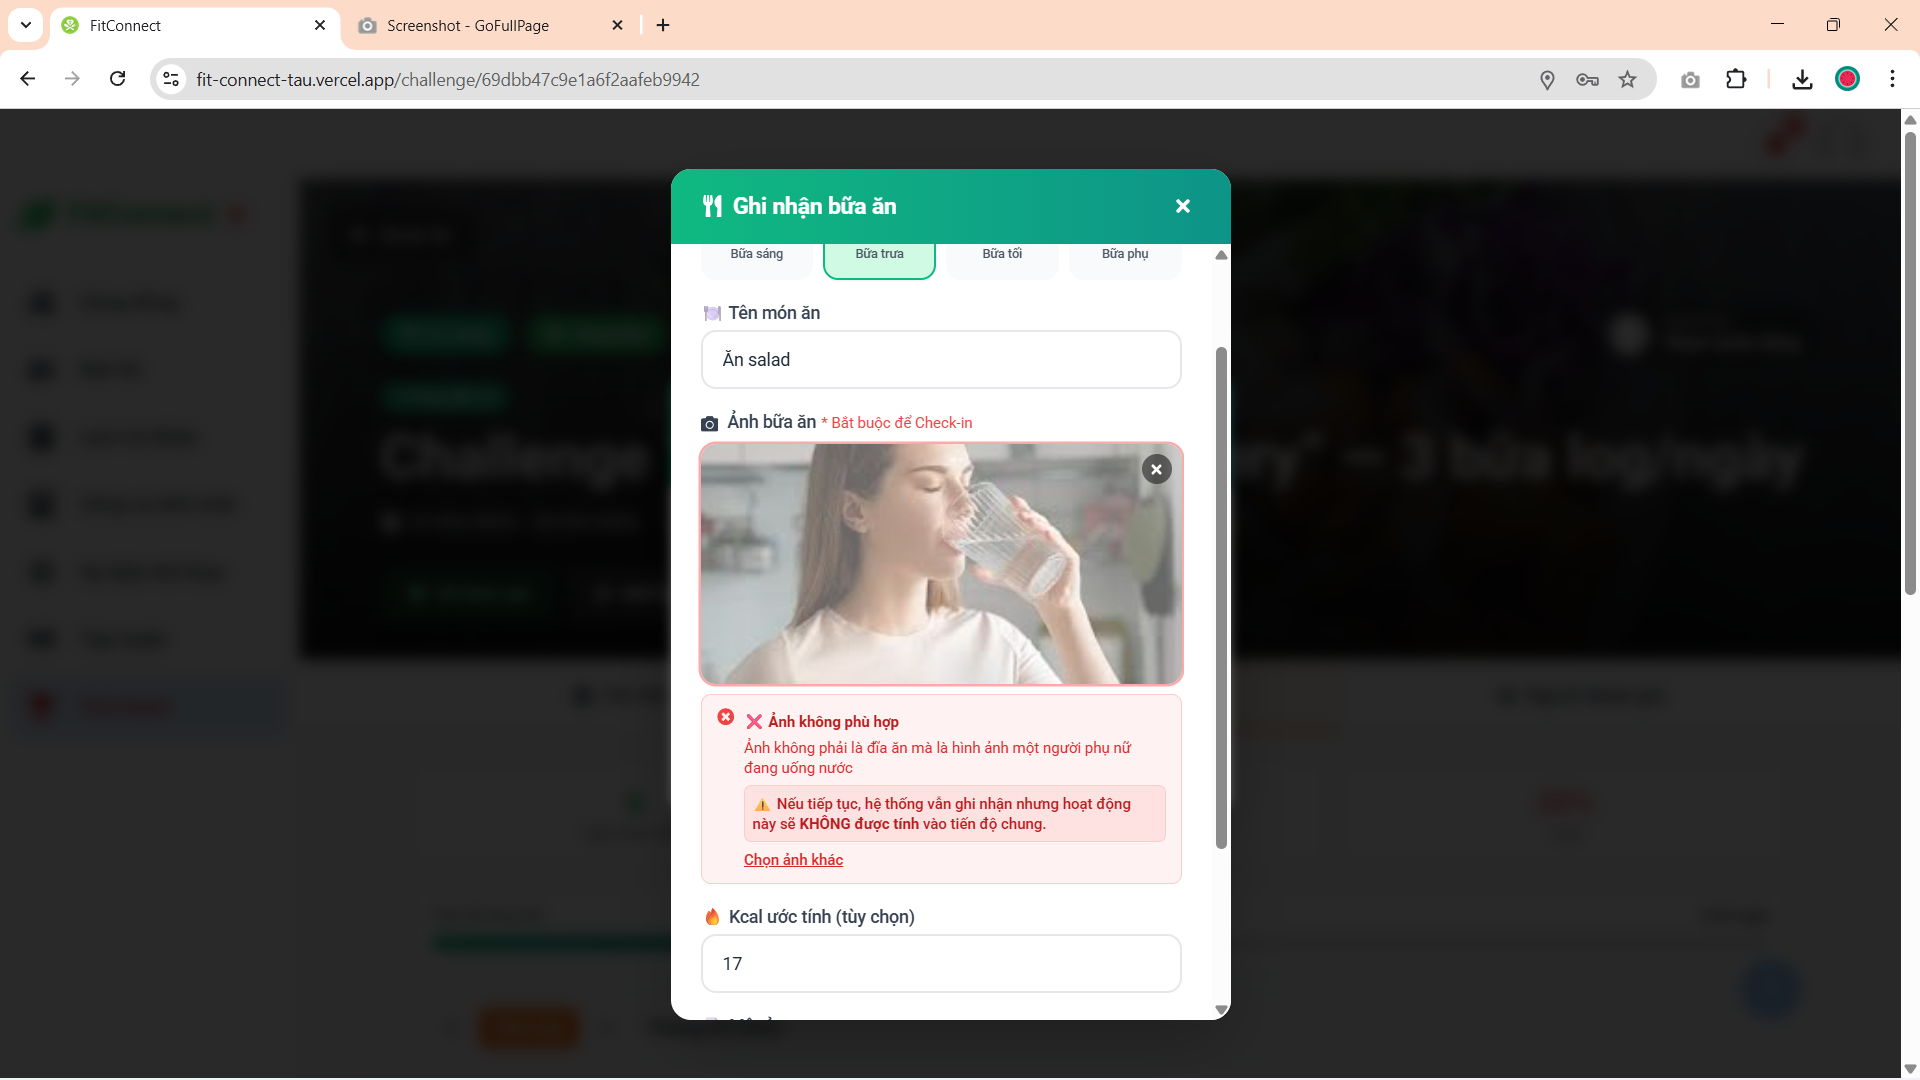
\includegraphics[width=0.60\textwidth]{Images/IMG/nhom4/1checkbuaankhonghople.png}
    \caption{Hệ thống AI xác minh ảnh bữa ăn không hợp lệ}
    \label{fig:impl_ch_food_invalid}
\end{figure}


    \item Sau khi Check-in bữa ăn hợp lệ, hệ thống hiển thị modal thông tin bữa ăn đã ghi nhận với badge ``AI Verified'', thông tin đóng góp (+1 bữa), năng lượng (kcal), nhận xét AI, và tiến độ hôm nay.

\begin{figure}[H]
    \centering
    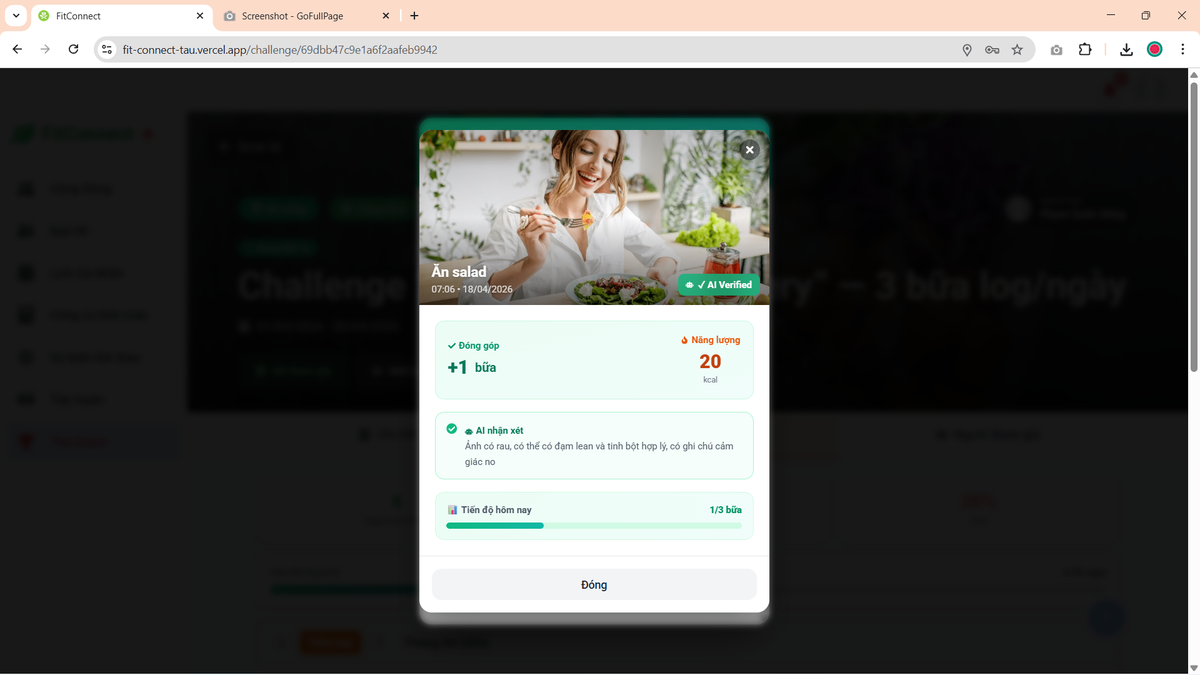
\includegraphics[width=0.60\textwidth]{Images/IMG/nhom4/1xemthongtinbuaandachecking.png}
    \caption{Hệ thống hiển thị thông tin bữa ăn đã được AI xác minh}
    \label{fig:impl_ch_food_verified}
\end{figure}


    \item Hệ thống cập nhật modal tiến độ ngày với bữa ăn hợp lệ được tính vào tiến độ (hiển thị xanh), bữa ăn không hợp lệ vẫn được ghi nhận nhưng hiển thị ghi chú ``Không hợp lệ'' và không tính vào tiến độ chung.

\begin{figure}[H]
    \centering
    \begin{subfigure}[b]{0.47\textwidth}
        \centering
        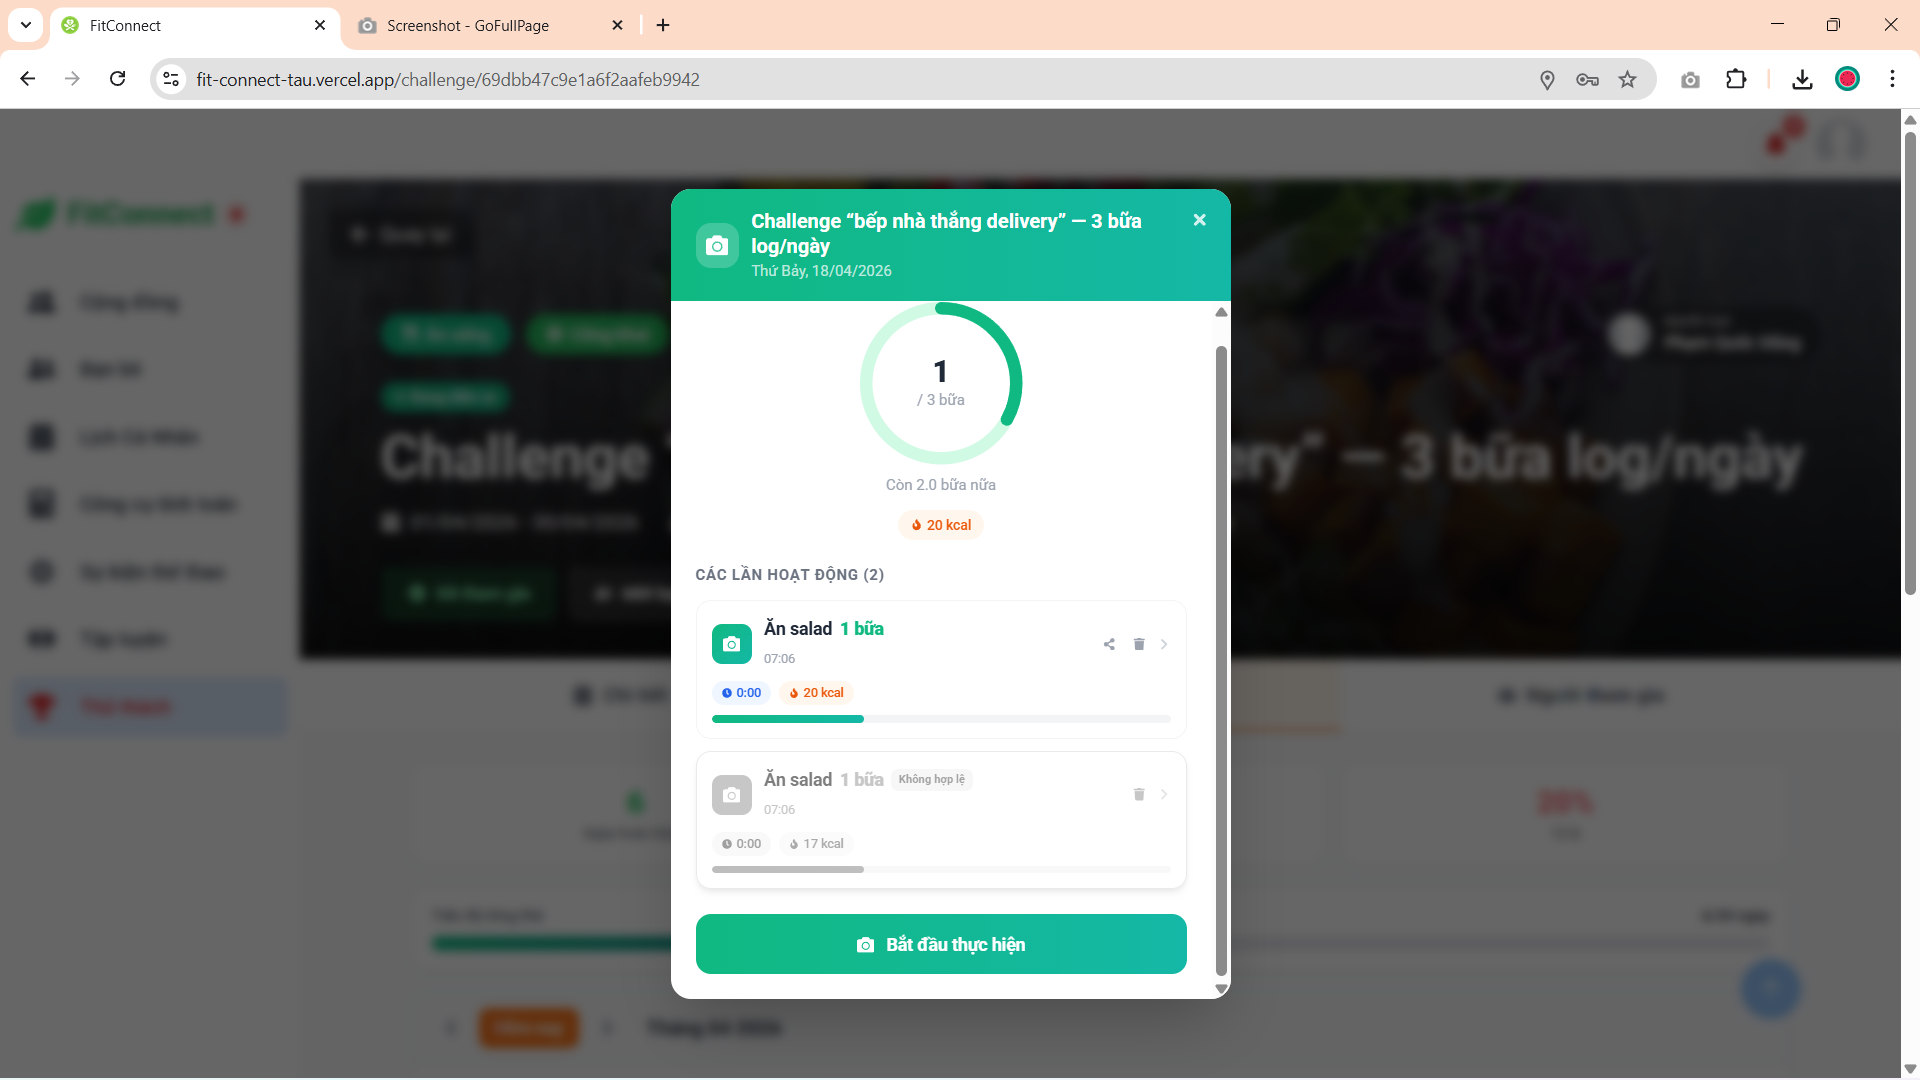
\includegraphics[width=\textwidth]{Images/IMG/nhom4/1modalcapnhatbuaanhople.png}
        \caption{Hệ thống cập nhật tiến độ ngày với bữa ăn hợp lệ}
        \label{fig:impl_ch_food_progress_valid}
    \end{subfigure}
    \hfill
    \begin{subfigure}[b]{0.47\textwidth}
        \centering
        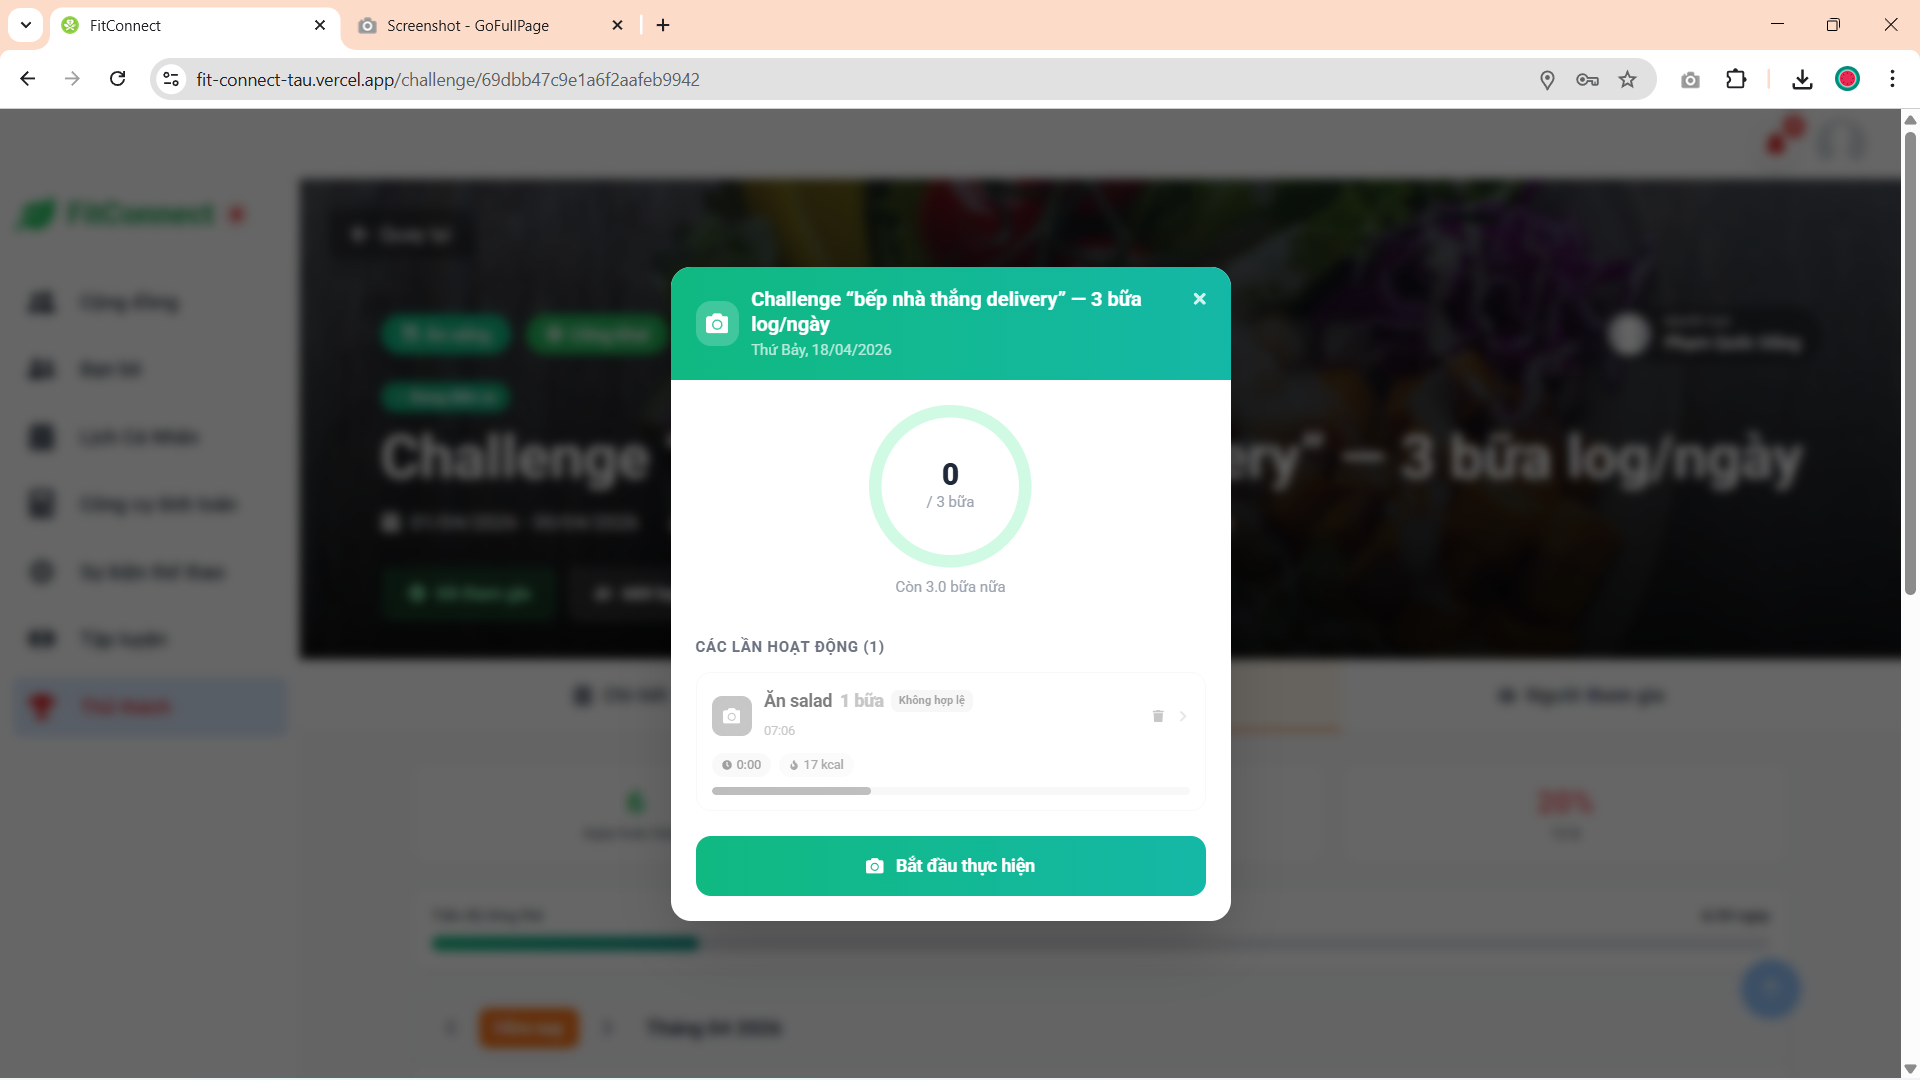
\includegraphics[width=\textwidth]{Images/IMG/nhom4/1tiendokhcapnhatbuaankhhople.png}
        \caption{Hệ thống hiển thị tiến độ khi có bữa ăn không hợp lệ không được tính}
        \label{fig:impl_ch_food_progress_invalid}
    \end{subfigure}
\end{figure}

\end{itemize}

\textbf{c) Đối với thử thách Thể dục (Workout, tập gym,...):}
\begin{itemize}
    \item Người tham gia nhấn vào ngày hiện tại trên lịch tiến độ, hệ thống hiển thị modal bắt đầu thực hiện với thông tin mục tiêu ngày (số bài tập), danh sách bài tập yêu cầu và nút Bắt đầu thực hiện.

\begin{figure}[H]
    \centering
    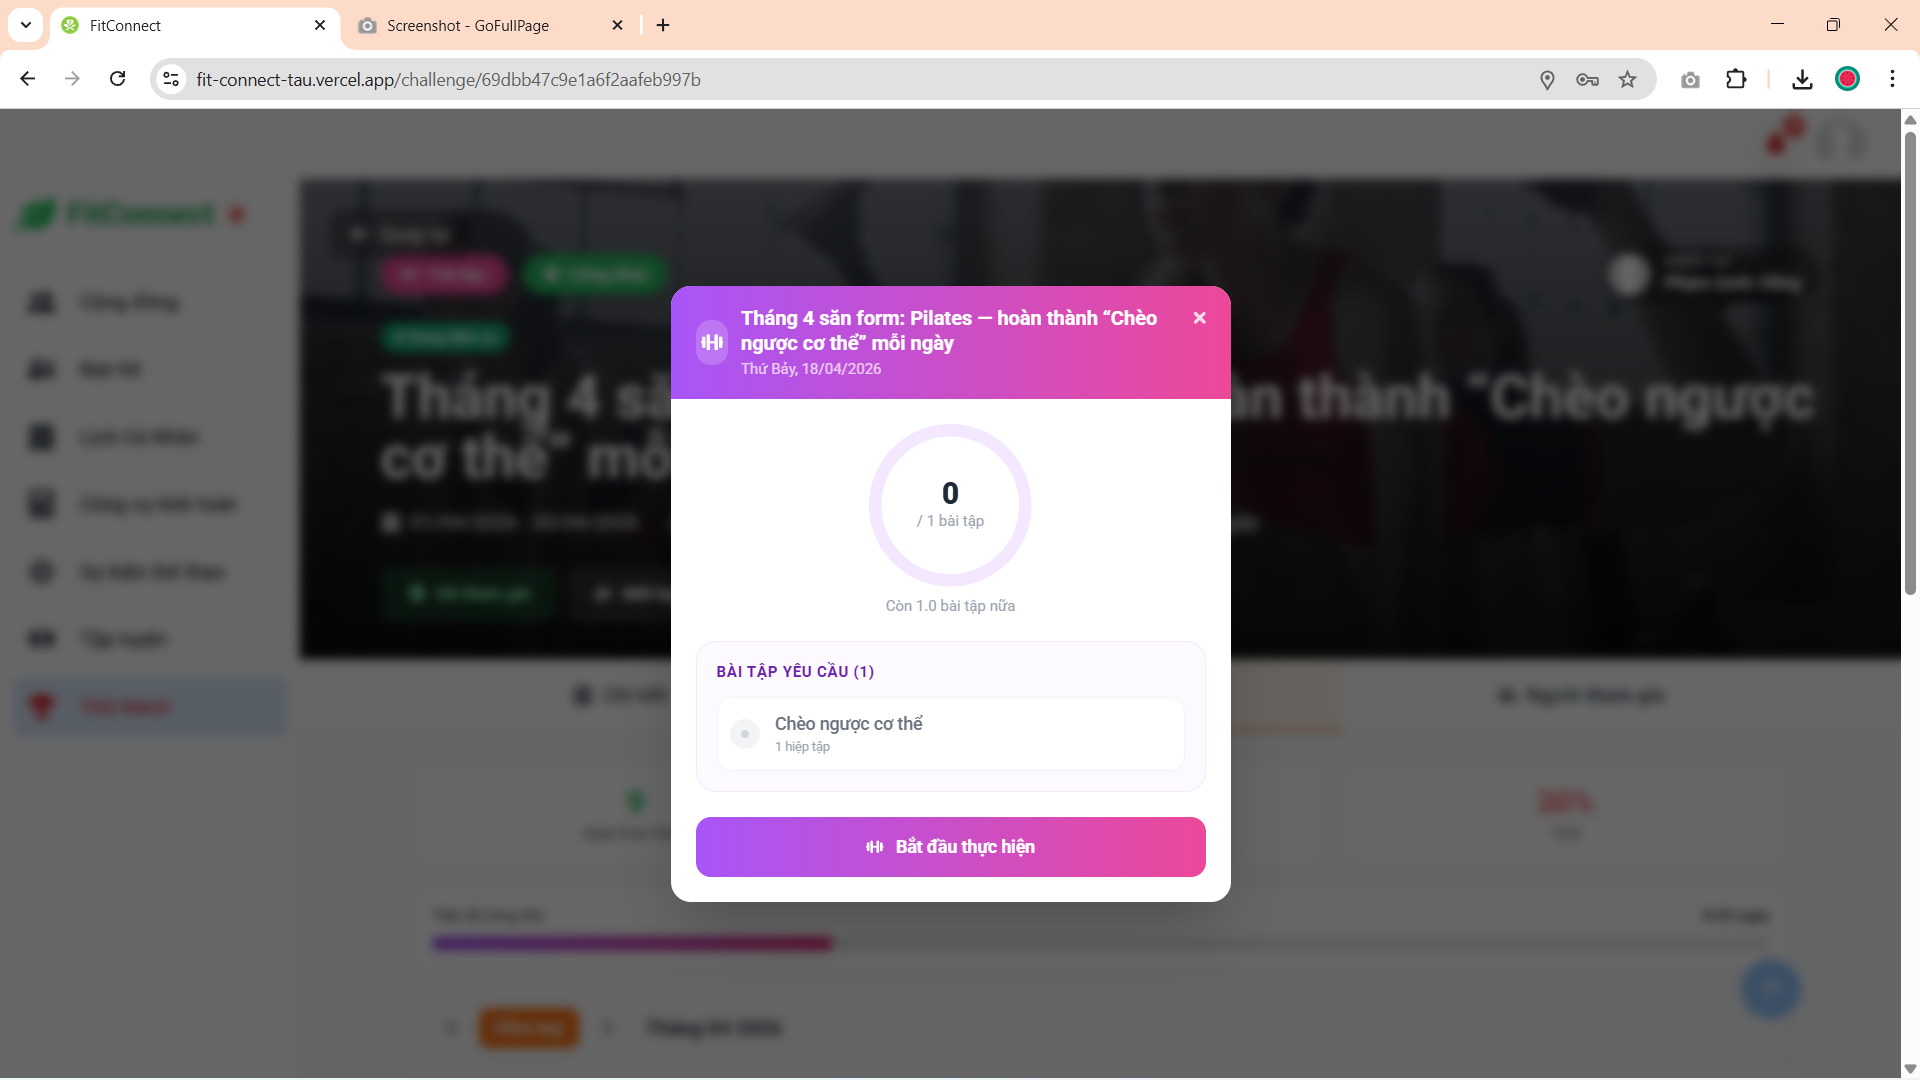
\includegraphics[width=0.60\textwidth]{Images/IMG/nhom4/1modalbatdauthuthachtapluyen.png}
    \caption{Hệ thống hiển thị modal bắt đầu thực hiện thử thách tập luyện}
    \label{fig:impl_ch_exercise_start}
\end{figure}


    \item Khi nhấn Bắt đầu thực hiện, hệ thống chuyển sang trang Chuẩn bị tập luyện gồm 2 bước: Bước 1 -- Chuẩn bị (chỉnh sửa set tập, số lần, mức tạ, kcal cho từng bài tập); Bước 2 -- Tập luyện (thực hiện và theo dõi tiến độ).

\begin{figure}[H]
    \centering
    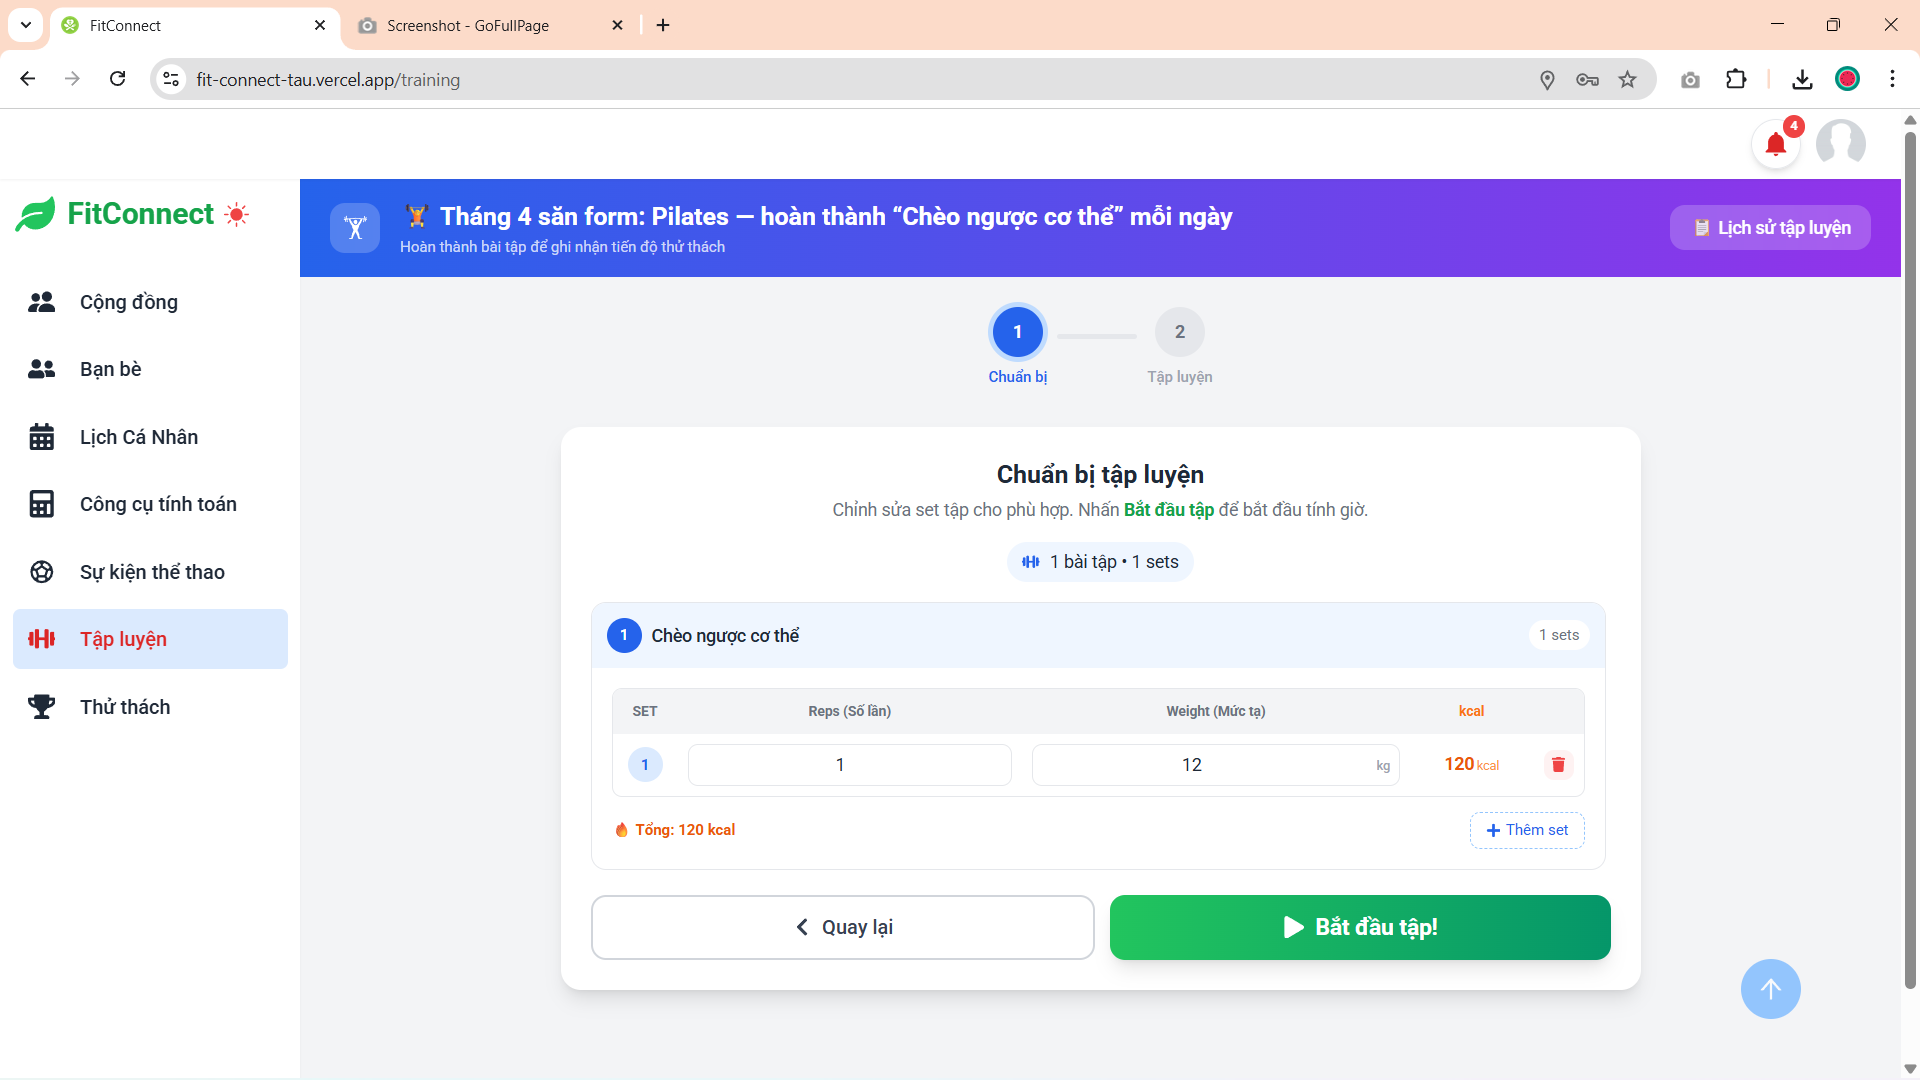
\includegraphics[width=0.60\textwidth]{Images/IMG/nhom4/1chuyenquatrangchuanbitapluyen.png}
    \caption{Người tham gia chuẩn bị tập luyện -- chỉnh sửa set tập}
    \label{fig:impl_ch_exercise_prep}
\end{figure}


    \item Sau khi nhấn Bắt đầu tập, hệ thống chuyển sang bước Tập luyện hiển thị bộ đếm thời gian, số bài tập hoàn thành, kcal đã đốt, và chi tiết từng bài tập (số lần, mức tạ, kcal). Người tham gia đánh dấu hoàn thành từng set và nhấn Hoàn thành tập luyện khi xong.

\begin{figure}[H]
    \centering
    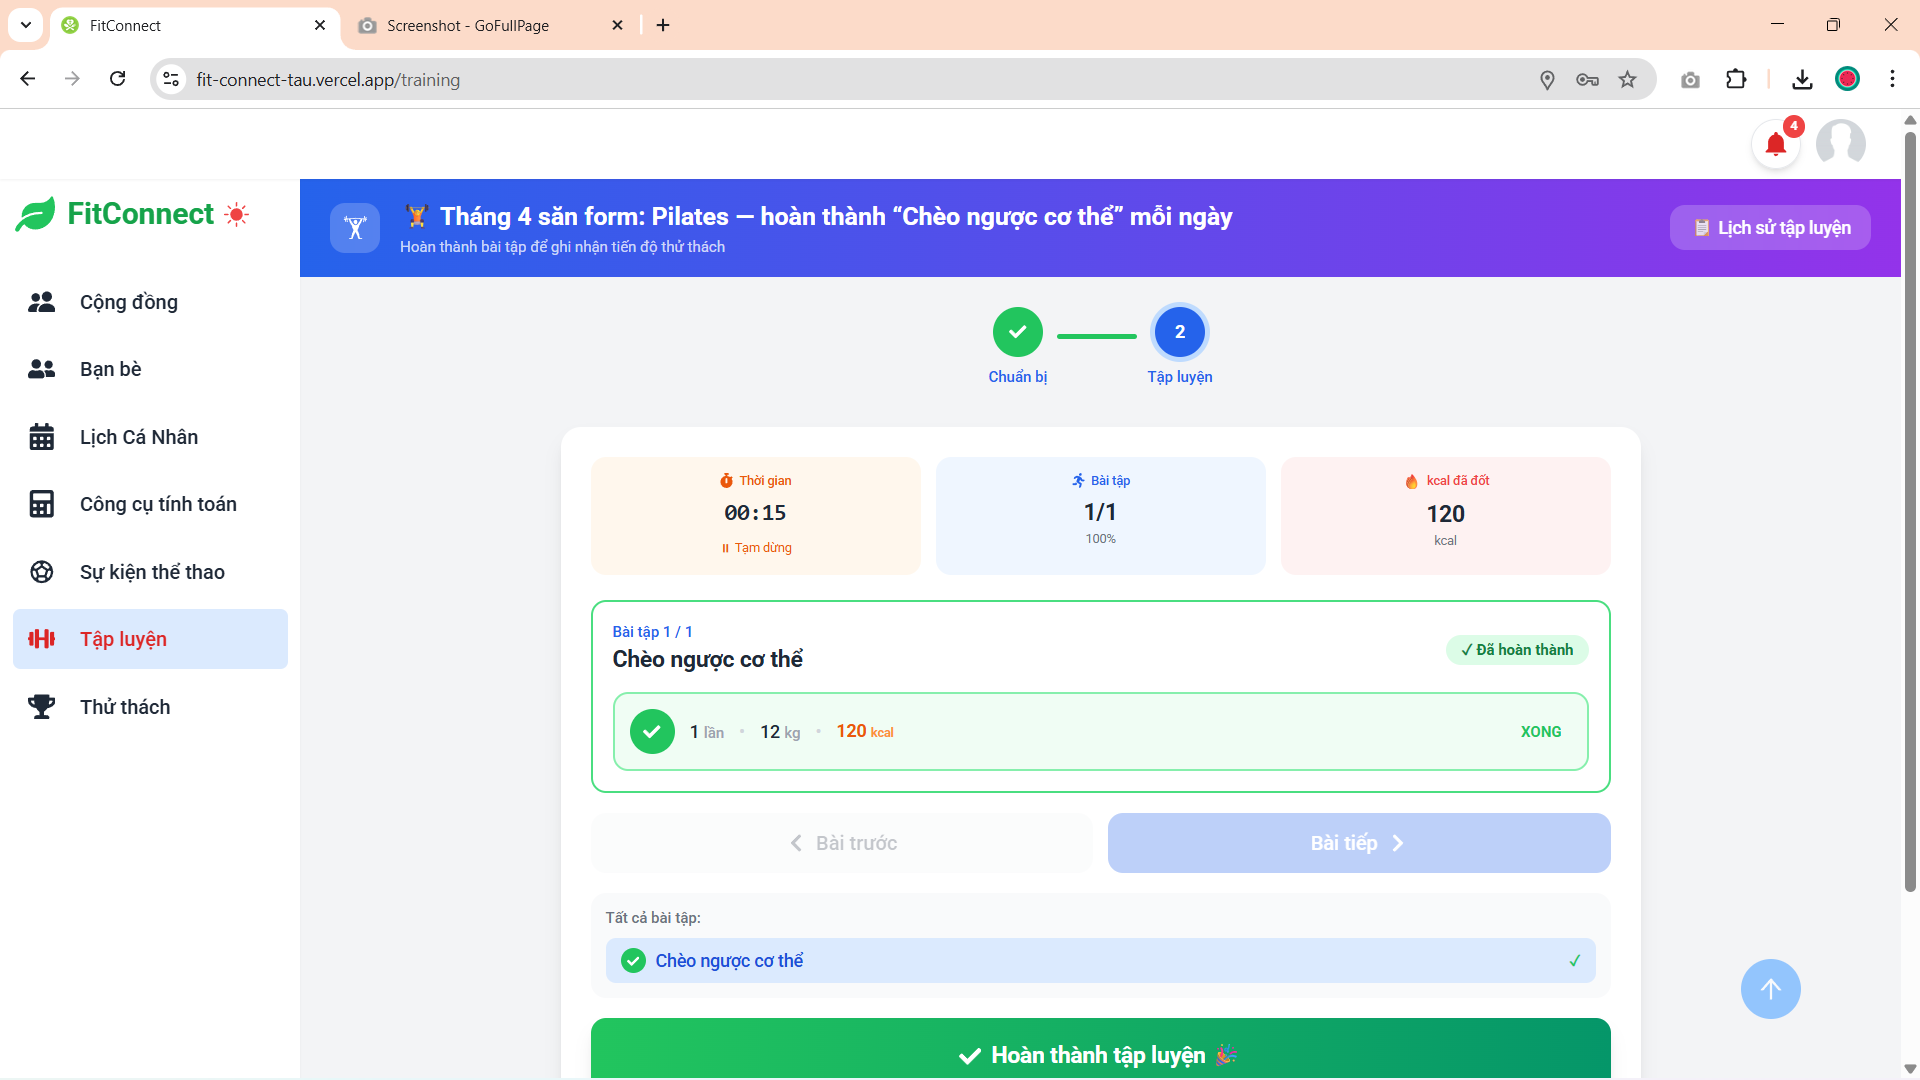
\includegraphics[width=0.60\textwidth]{Images/IMG/nhom4/1chuyenquabuoctapluyen.png}
    \caption{Người tham gia thực hiện tập luyện và theo dõi tiến độ}
    \label{fig:impl_ch_exercise_training}
\end{figure}


    \item Sau khi hoàn thành tập luyện, hệ thống quay lại modal tiến độ ngày hiển thị trạng thái ``Hoàn thành!'' với tổng hợp: thời gian, kcal đốt, danh sách bài tập đã xong và lịch sử các lần hoạt động trong ngày.

\end{itemize}

\textbf{Chia sẻ hoạt động thử thách:}
\begin{itemize}
    \item Người tham gia có thể chia sẻ hoạt động thử thách (tiến độ GPS, kết quả chạy bộ) lên trang Cộng đồng; hoạt động sẽ tự động xuất hiện dưới dạng bài viết trên Bảng tin kèm bản đồ lộ trình.

\begin{figure}[H]
    \centering
    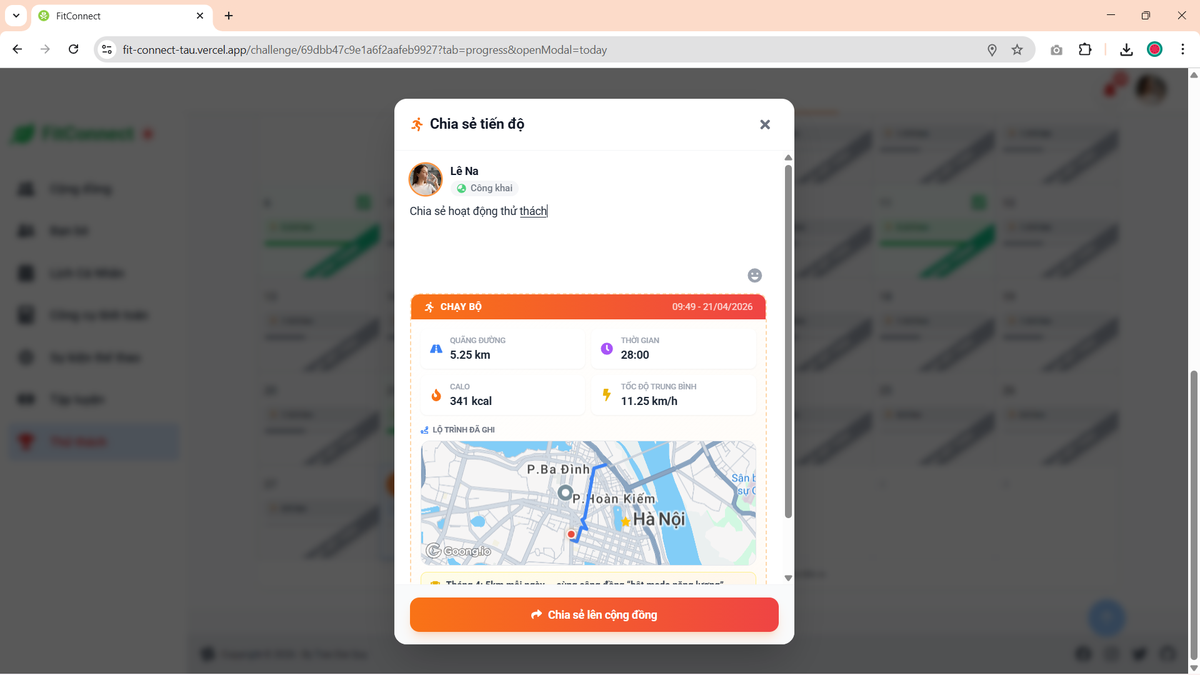
\includegraphics[width=0.60\textwidth]{Images/IMG/nhom4/chiasehoatdongthuthach.png}
    \caption{Người tham gia thao tác chia sẻ hoạt động thử thách lên cộng đồng}
    \label{fig:impl_ch_share_activity}
\end{figure}

\end{itemize}

\subsubsection{Luồng thao tác quản trị thử thách (Góc độ Quản trị viên)}
\begin{itemize}
    \item Quản trị viên truy cập trang Kiểm duyệt thử thách, hệ thống hiển thị danh sách thử thách bị báo cáo bao gồm thông tin: người tạo thử thách, tên thử thách, số báo cáo, người báo cáo, nội dung báo cáo và các hành động (xem chi tiết, giữ thử thách, gỡ thử thách).

\begin{figure}[H]
    \centering
    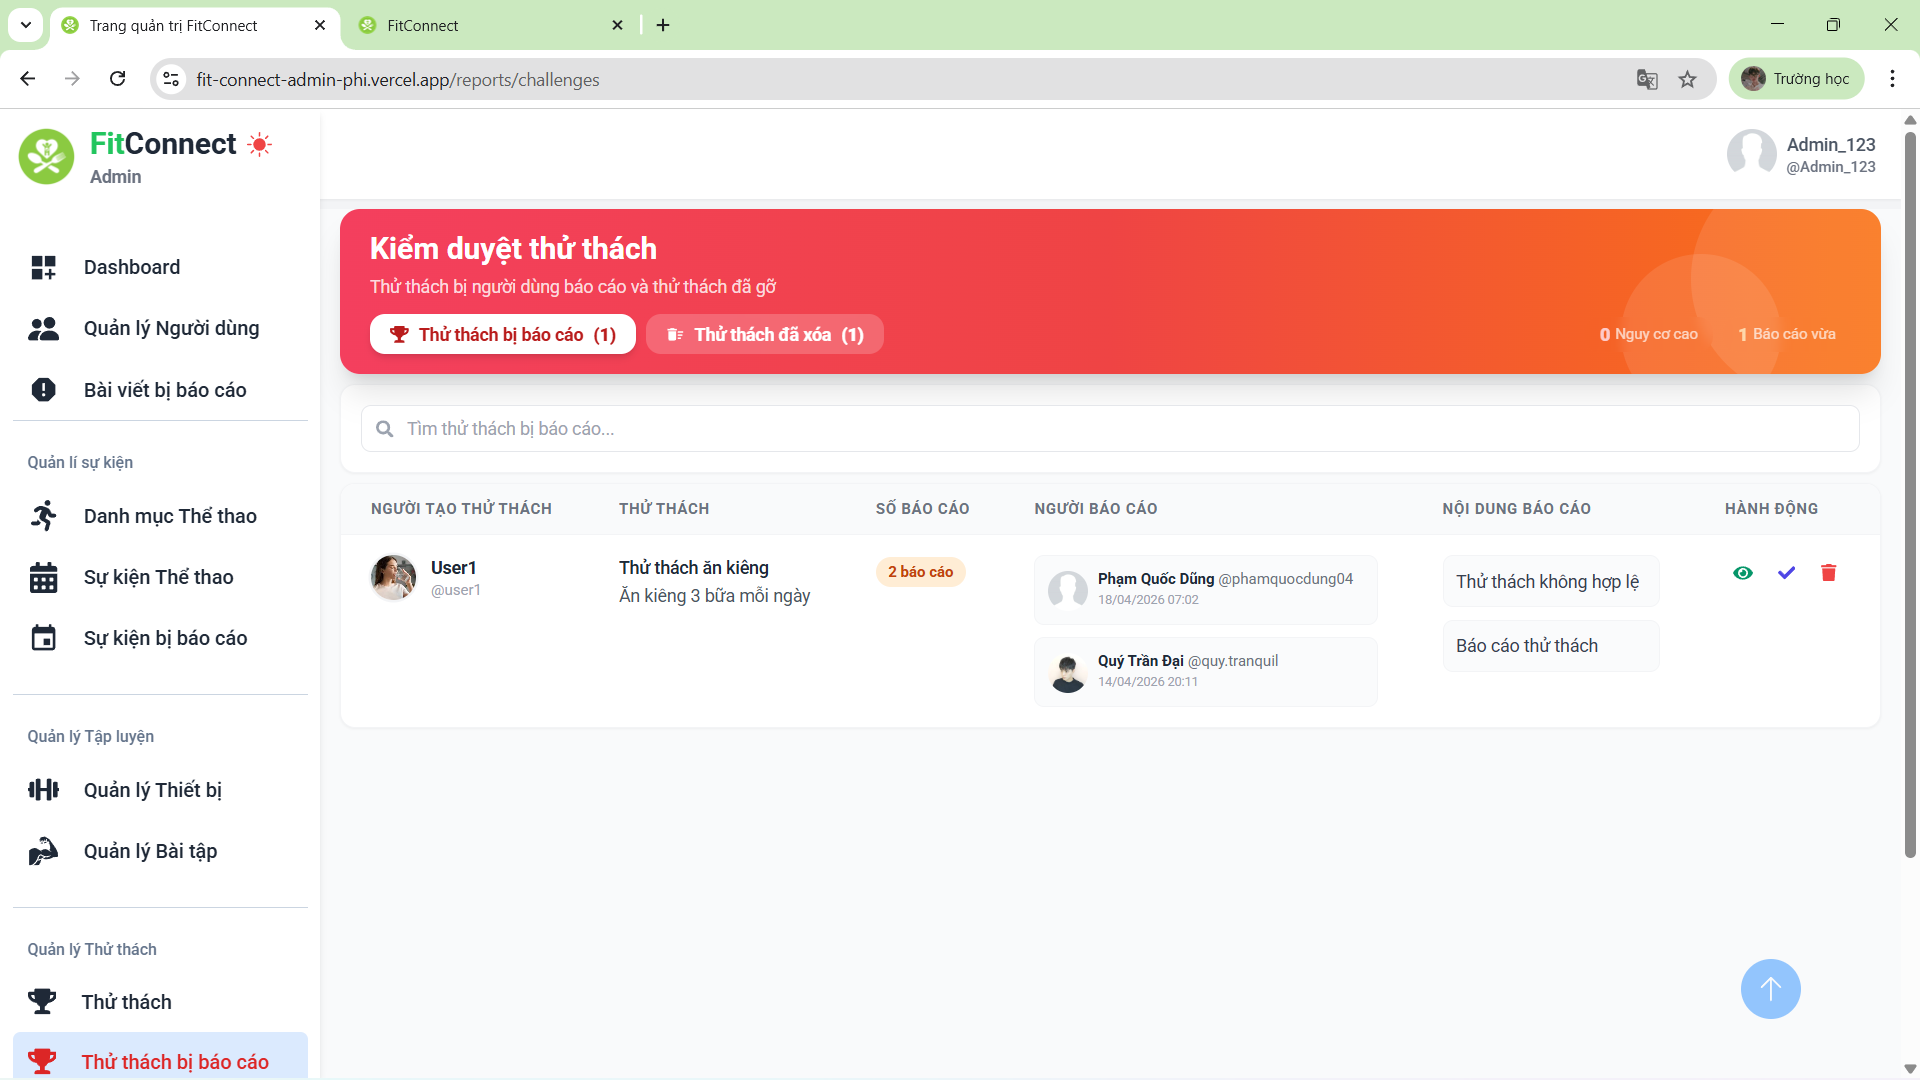
\includegraphics[width=0.60\textwidth]{Images/IMG/nhom4/adminxemthuthachbibaocao.png}
    \caption{Quản trị viên xem danh sách thử thách bị báo cáo}
    \label{fig:impl_ch_admin_list}
\end{figure}


    \item Quản trị viên có thể nhấn xem chi tiết để xem thông tin thử thách bị báo cáo bao gồm: tên thử thách, trạng thái, thời gian diễn ra, số người tham gia, danh sách người báo cáo và thông tin chi tiết thử thách.

\begin{figure}[H]
    \centering
    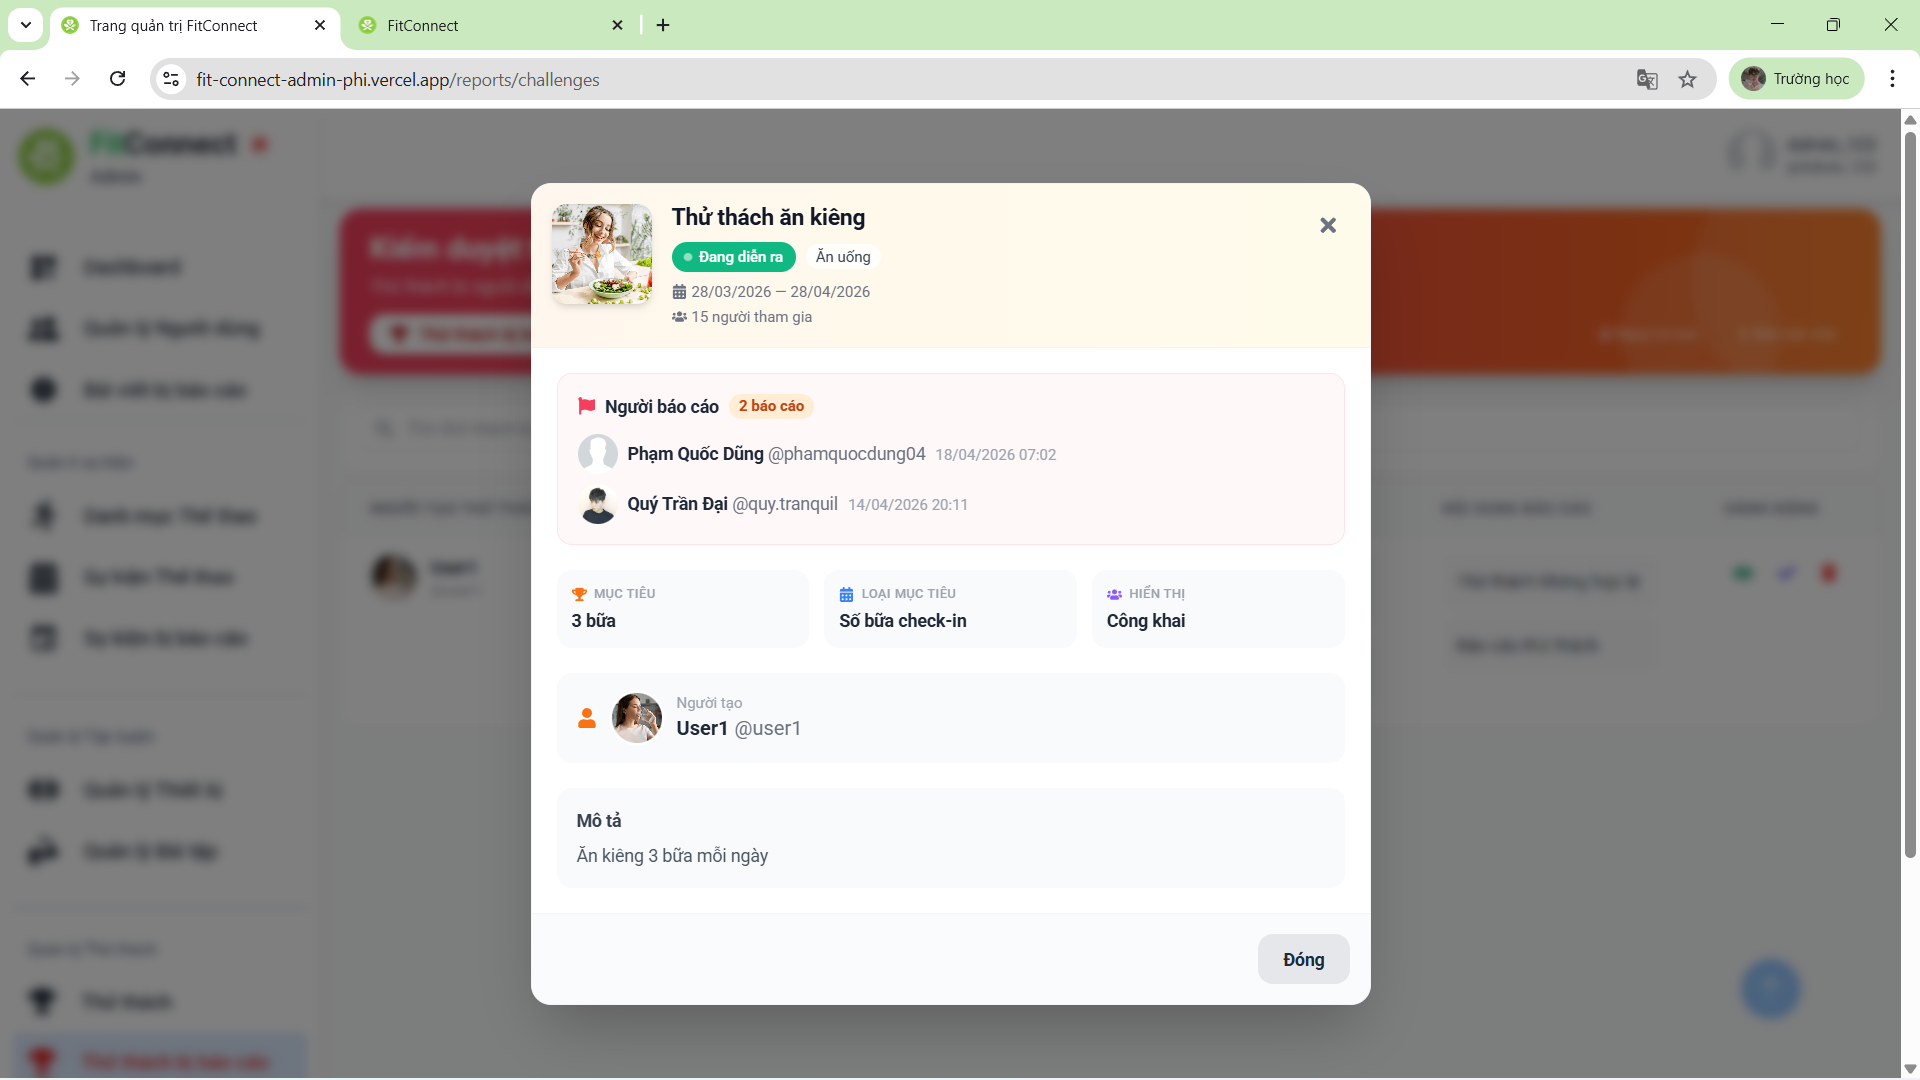
\includegraphics[width=0.60\textwidth]{Images/IMG/nhom4/adminxemthongtinthuthachbaoca.png}
    \caption{Quản trị viên xem thông tin chi tiết thử thách bị báo cáo}
    \label{fig:impl_ch_admin_view}
\end{figure}


    \item Quản trị viên xử lý thử thách bị báo cáo theo hai hướng: \textbf{Giữ lại} (thử thách tiếp tục hiển thị bình thường) hoặc \textbf{Gỡ} (thử thách bị ẩn và chuyển vào danh sách đã xóa). Tại tab ``Đã xóa'', Quản trị viên có thể xem xét và khôi phục thử thách nếu cần.

\begin{figure}[H]
    \centering
    \begin{subfigure}[b]{0.47\textwidth}
        \centering
        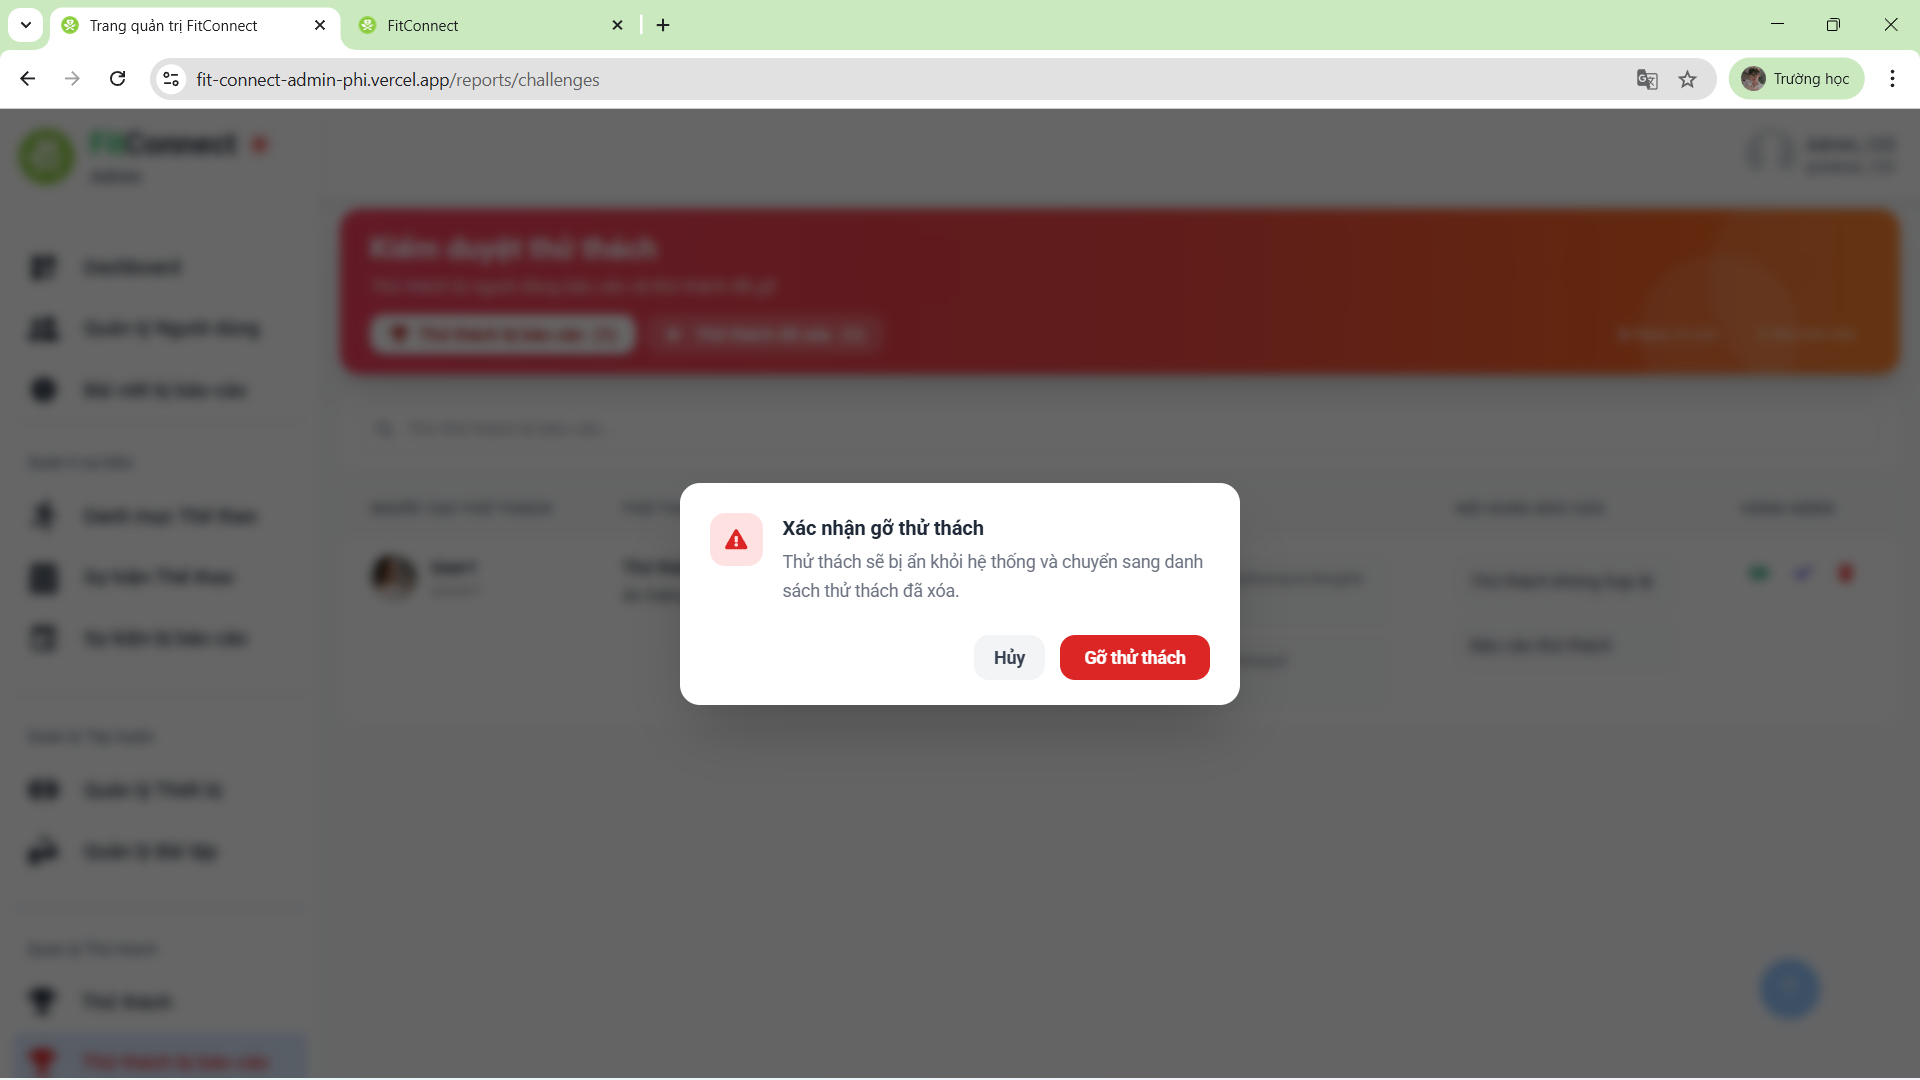
\includegraphics[width=\textwidth]{Images/IMG/nhom4/adminxoathuthach.png}
        \caption{Gỡ thử thách vi phạm khỏi cộng đồng}
        \label{fig:impl_ch_admin_delete}
    \end{subfigure}
    \hfill
    \begin{subfigure}[b]{0.47\textwidth}
        \centering
        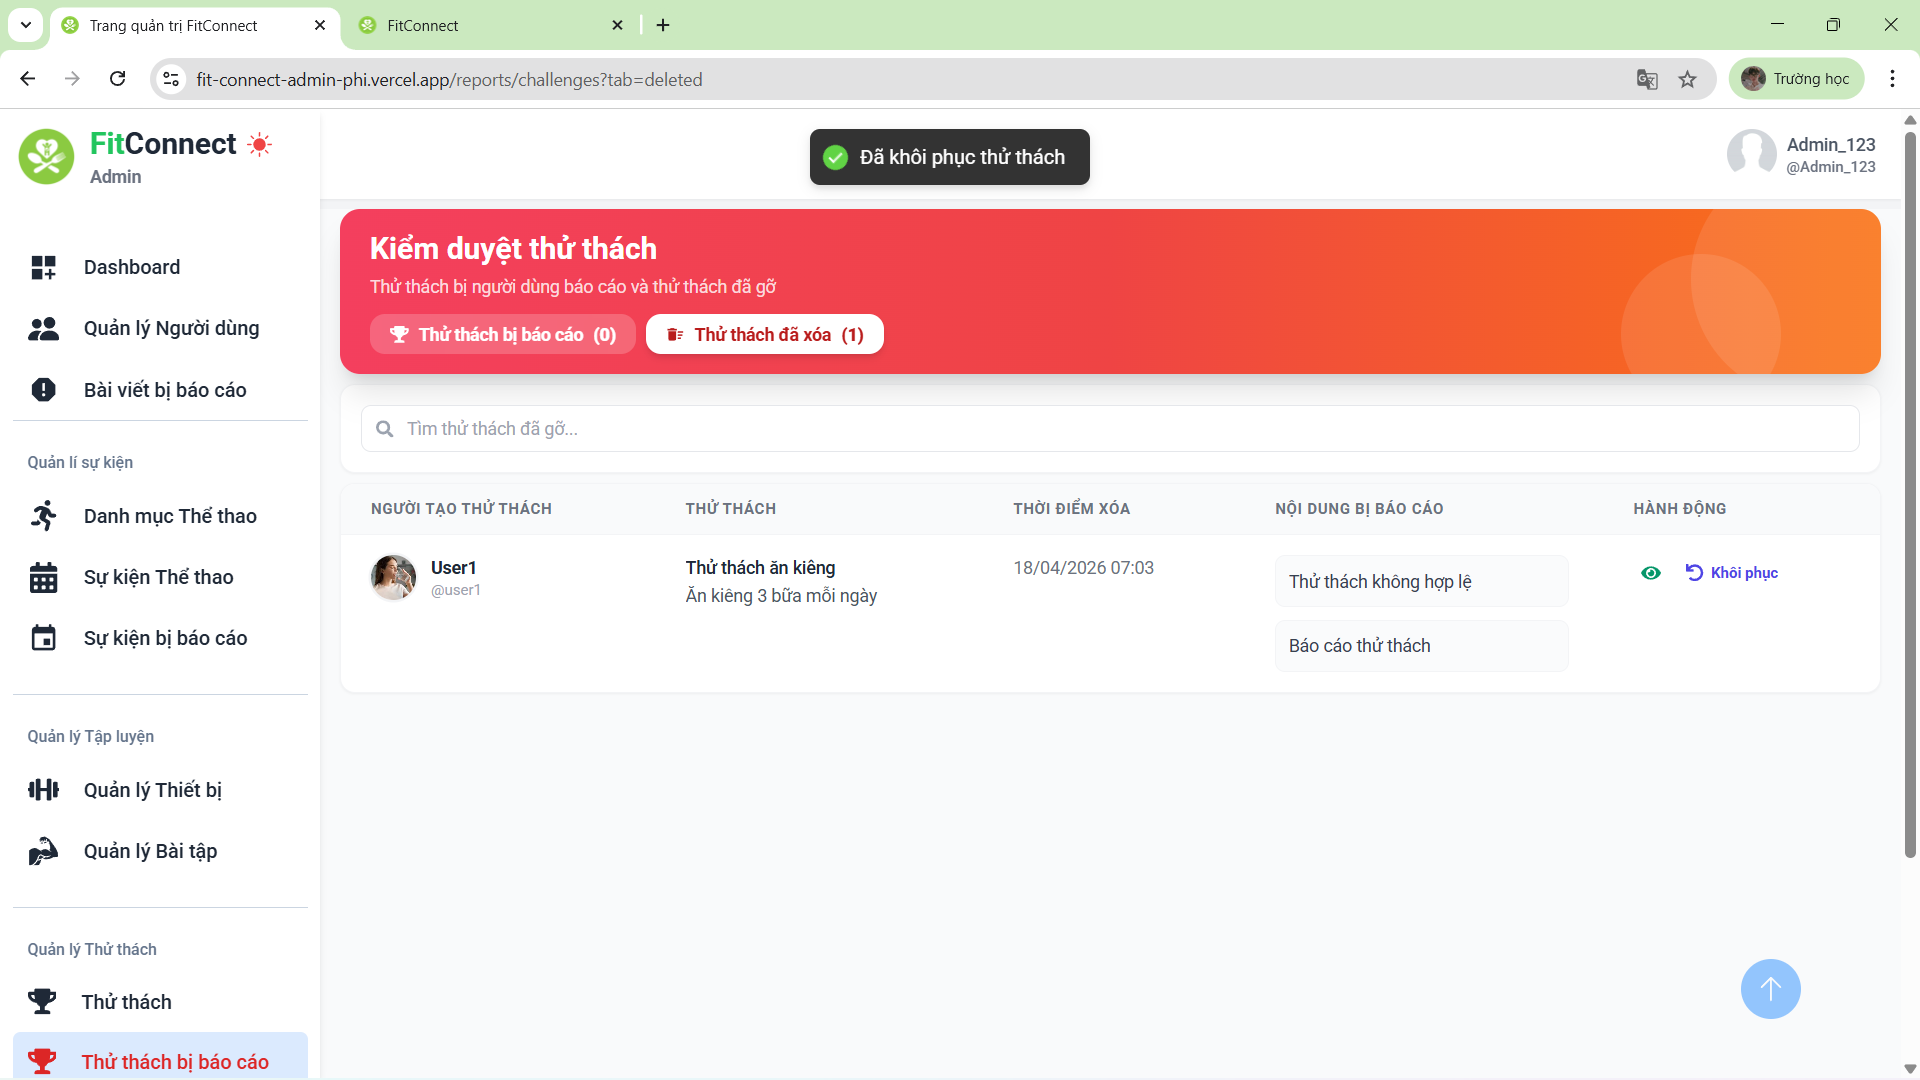
\includegraphics[width=\textwidth]{Images/IMG/nhom4/adminxemthuthachdaxoa.png}
        \caption{Danh sách thử thách đã xóa và tùy chọn khôi phục}
        \label{fig:impl_ch_admin_deleted_list}
    \end{subfigure}
    \vspace{0.3em}
    \caption{Quản trị viên xử lý và quản lý thử thách vi phạm}
    \label{fig:impl_ch_admin_moderation}
\end{figure}

\end{itemize}

\subsection{Nhóm tính năng Tính toán chỉ số sức khỏe}
\label{subsec:impl_health_calculator}

Nhóm tính năng Tính toán chỉ số sức khỏe cung cấp cho người dùng bộ công cụ toàn diện để đo lường, theo dõi và phân tích các chỉ số thể chất cá nhân. Hệ thống hỗ trợ 8 công cụ tính toán: BMI (Body Mass Index -- Chỉ số khối cơ thể), TDEE (Total Daily Energy Expenditure -- Tổng năng lượng tiêu thụ mỗi ngày), Body Fat (Phần trăm mỡ cơ thể), BMR (Basal Metabolic Rate -- Tỷ lệ trao đổi chất cơ bản), IBW (Ideal Body Weight -- Cân nặng lý tưởng), LBM (Lean Body Mass -- Khối lượng cơ nạc), Calories Burned (Lượng calories đốt cháy) và Water Need (Nhu cầu nước hàng ngày). Điểm nổi bật của hệ thống là sự tích hợp AI để phân tích sức khỏe và gợi ý bài tập phù hợp ngay từ kết quả tính toán, đồng thời lưu trữ lịch sử chỉ số để người dùng theo dõi sự thay đổi theo thời gian.

\subsubsection{Luồng tính toán và phân tích chỉ số sức khỏe}

\begin{itemize}
    \item Người dùng truy cập trang Công cụ tính toán từ thanh điều hướng bên trái. Hệ thống hiển thị giao diện trang tính toán gồm 2 tab: ``Công cụ tính'' và ``Lịch sử chỉ số''. Tại tab Công cụ tính, hệ thống hiển thị danh sách 8 công cụ tính toán sức khỏe, mỗi công cụ gồm tên viết tắt, tên đầy đủ, mô tả ngắn gọn và nút ``Tính ngay''.

\begin{figure}[H]
    \centering
    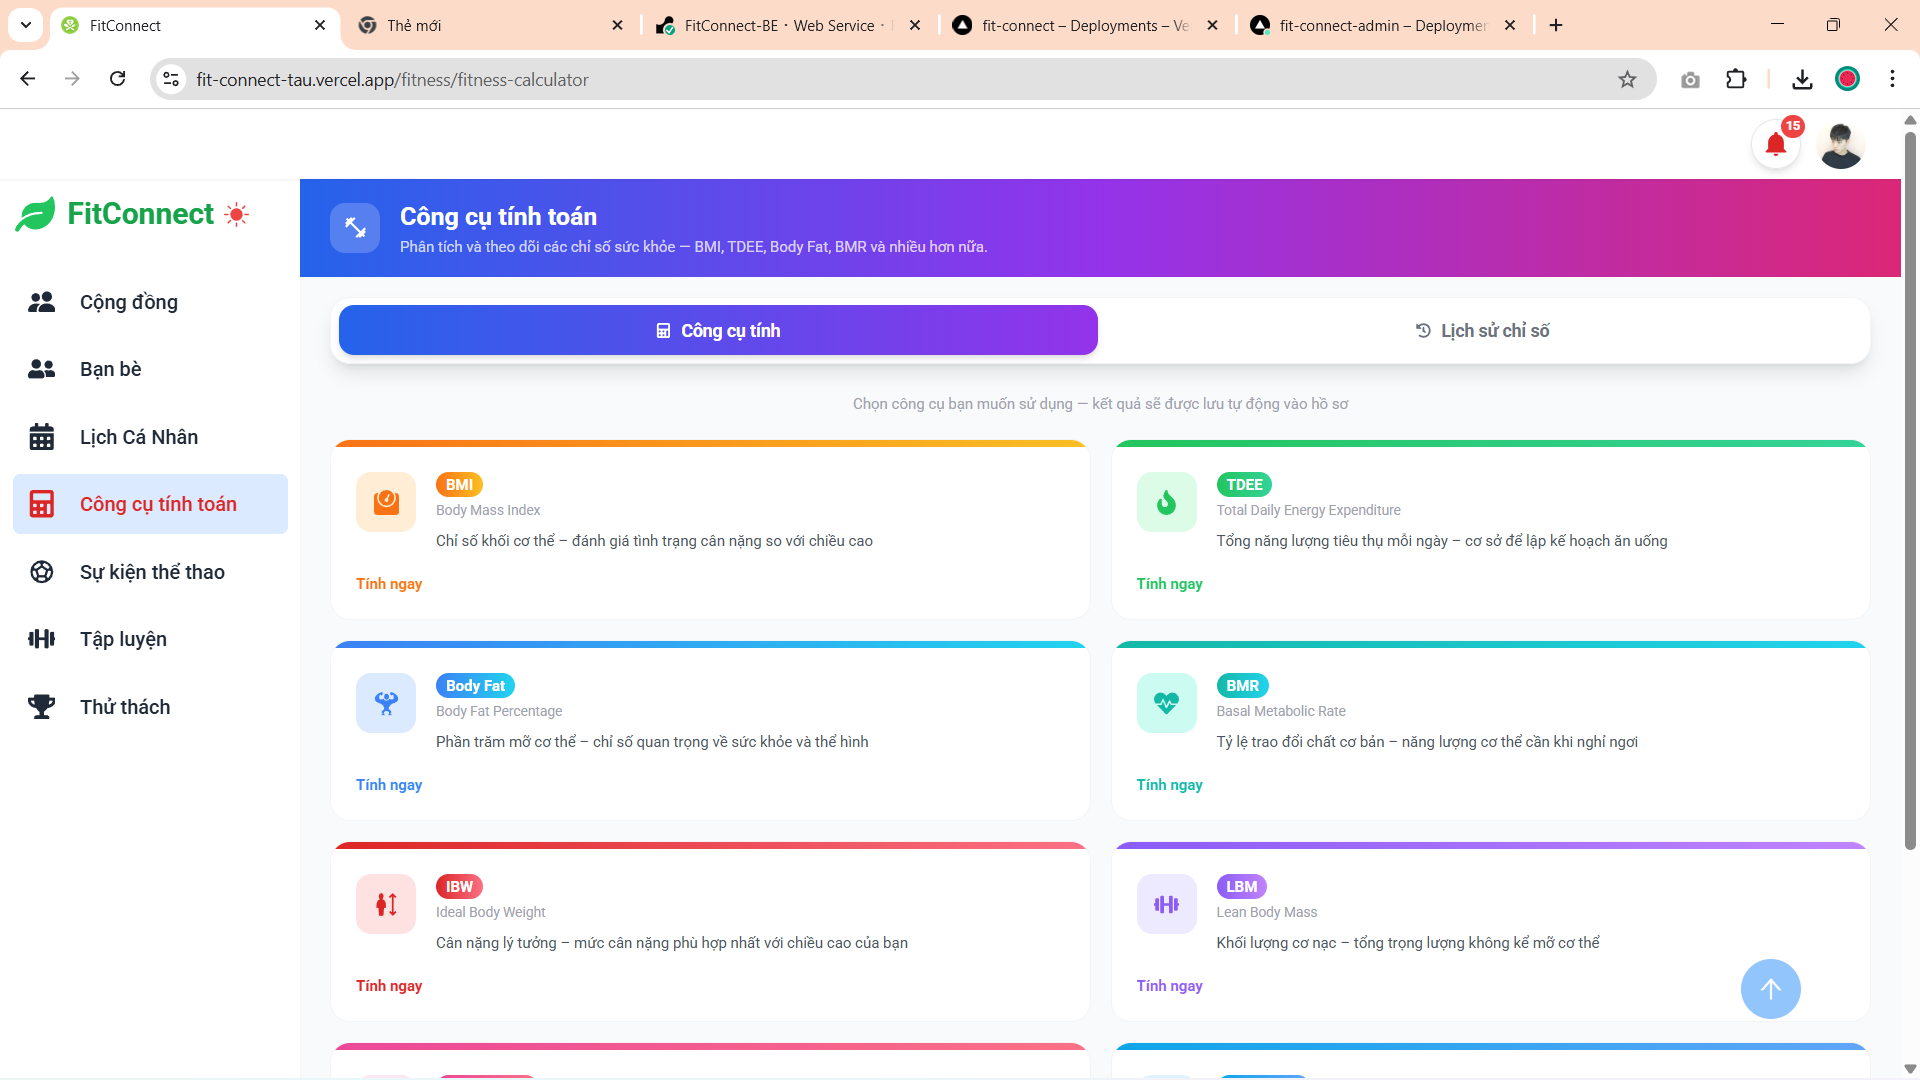
\includegraphics[width=0.60\textwidth]{Images/IMG/nhom6/giaodientrangtinhtoanchiso.png}
    \caption{Hệ thống hiển thị trang Công cụ tính toán chỉ số sức khỏe}
    \label{fig:impl_calc_main}
\end{figure}


    \item Người dùng nhấn ``Tính ngay'' vào một công cụ (ví dụ: BMI), hệ thống chuyển đến trang tính toán chi tiết của chỉ số đó. Tại đây, hệ thống hiển thị bài viết giải thích chi tiết về chỉ số (định nghĩa, công thức, ý nghĩa), biểu mẫu nhập dữ liệu (chiều cao, cân nặng, tuổi, giới tính tùy theo loại chỉ số) và kết quả tính toán kèm đánh giá trực quan (thanh màu phân vùng, phân loại tình trạng). Kết quả sau khi tính được tự động lưu vào hồ sơ cá nhân của người dùng.

    \item Sau khi có kết quả, người dùng có thể nhấn nút ``AI Phân Tích Sức Khỏe''. Hệ thống gửi các chỉ số sức khỏe hiện tại tới AI, AI phân tích và trả về modal hiển thị: phần ``Đánh giá sức khỏe'' với nhận xét chi tiết về tình trạng sức khỏe dựa trên chỉ số, và phần ``Bài tập được gợi ý'' với danh sách các bài tập phù hợp từ kho bài tập hệ thống kèm nhãn mức độ (Dễ, Trung bình), loại bài tập (Sức mạnh, Cardio) và lý do AI gợi ý cho từng bài.

\begin{figure}[H]
    \centering
    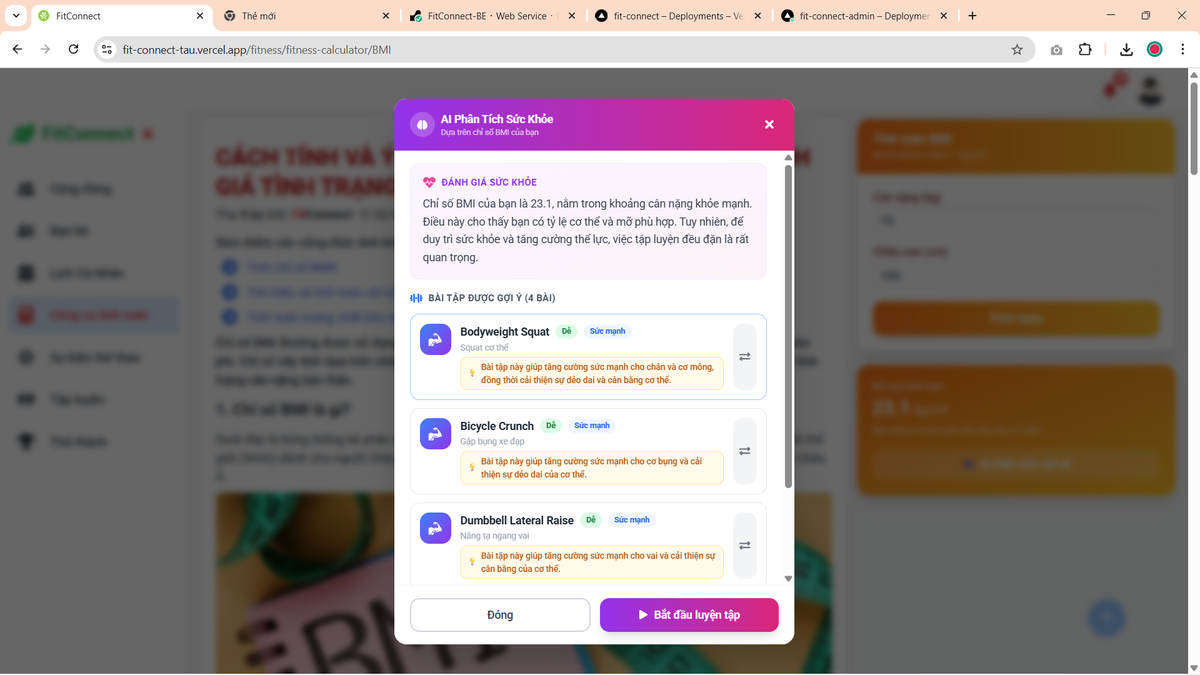
\includegraphics[width=0.60\textwidth]{Images/IMG/nhom6/AIphantichsuckhoa.png}
    \caption{Hệ thống AI phân tích sức khỏe và gợi ý bài tập dựa trên chỉ số BMI}
    \label{fig:impl_calc_ai}
\end{figure}


    \item Người dùng có thể chọn các bài tập gợi ý và nhấn ``Bắt đầu luyện tập''. Hệ thống chuyển sang trang Chuẩn bị tập luyện hiển thị danh sách các bài tập đã chọn (ví dụ: 4 bài tập, 5 sets), cho phép người dùng chỉnh sửa số lần (Reps), mức tạ (Weight), thêm set trước khi bắt đầu. Hệ thống tự động tính kcal ước tính cho mỗi set. Người dùng cũng có thể nhấn ``Lưu bài tập'' để lưu giáo án tập luyện cho lần sau.

\begin{figure}[H]
    \centering
    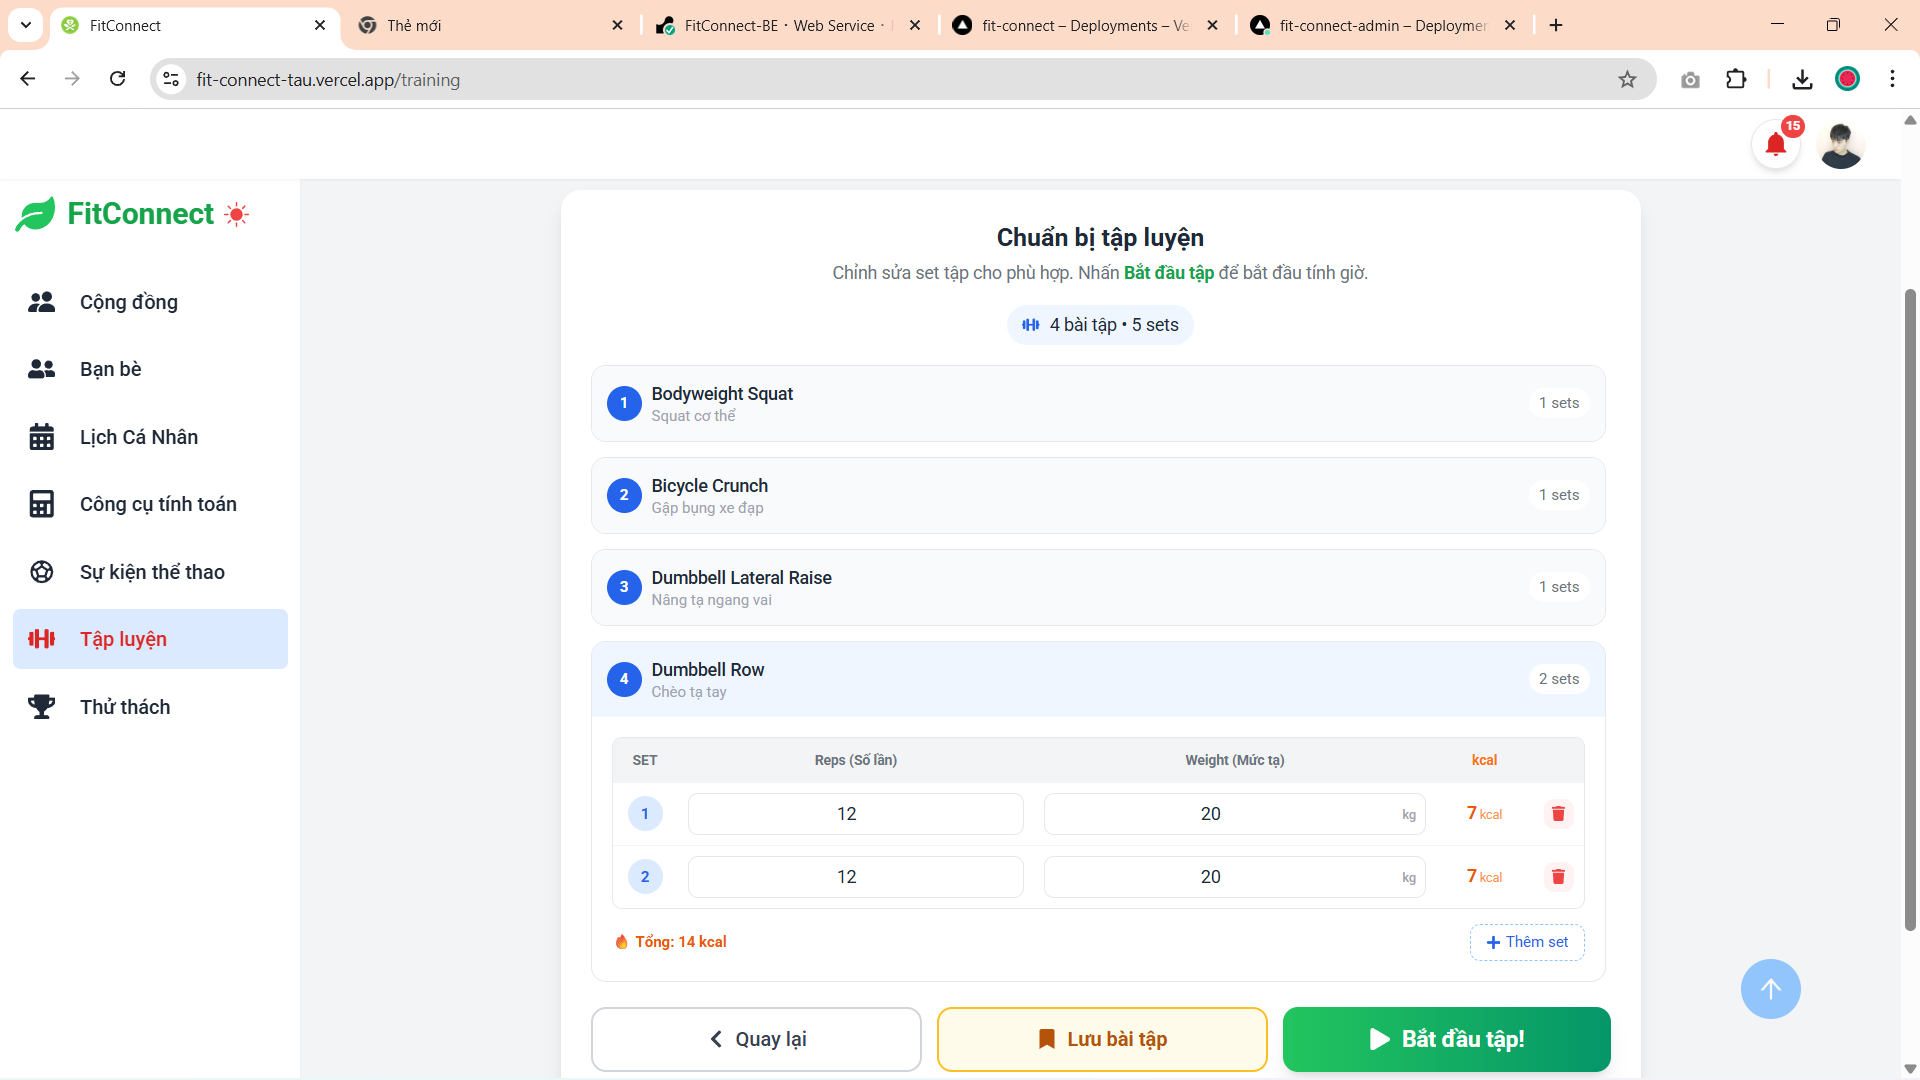
\includegraphics[width=0.60\textwidth]{Images/IMG/nhom6/chuyenquamanchuanbitapluyen.png}
    \caption{Người dùng chuẩn bị tập luyện với các bài tập được AI gợi ý}
    \label{fig:impl_calc_prep}
\end{figure}


    \item Khi nhấn ``Bắt đầu tập!'', hệ thống chuyển sang trang Tập luyện hiển thị bộ đếm thời gian thực, số bài tập hoàn thành (ví dụ: 0/4), kcal đã đốt, và chi tiết từng bài tập với thông tin set (số lần, mức tạ, kcal). Người dùng đánh dấu ``Xong'' cho từng set sau khi hoàn thành và nhấn ``Bài tiếp'' để chuyển sang bài tập tiếp theo.

\begin{figure}[H]
    \centering
    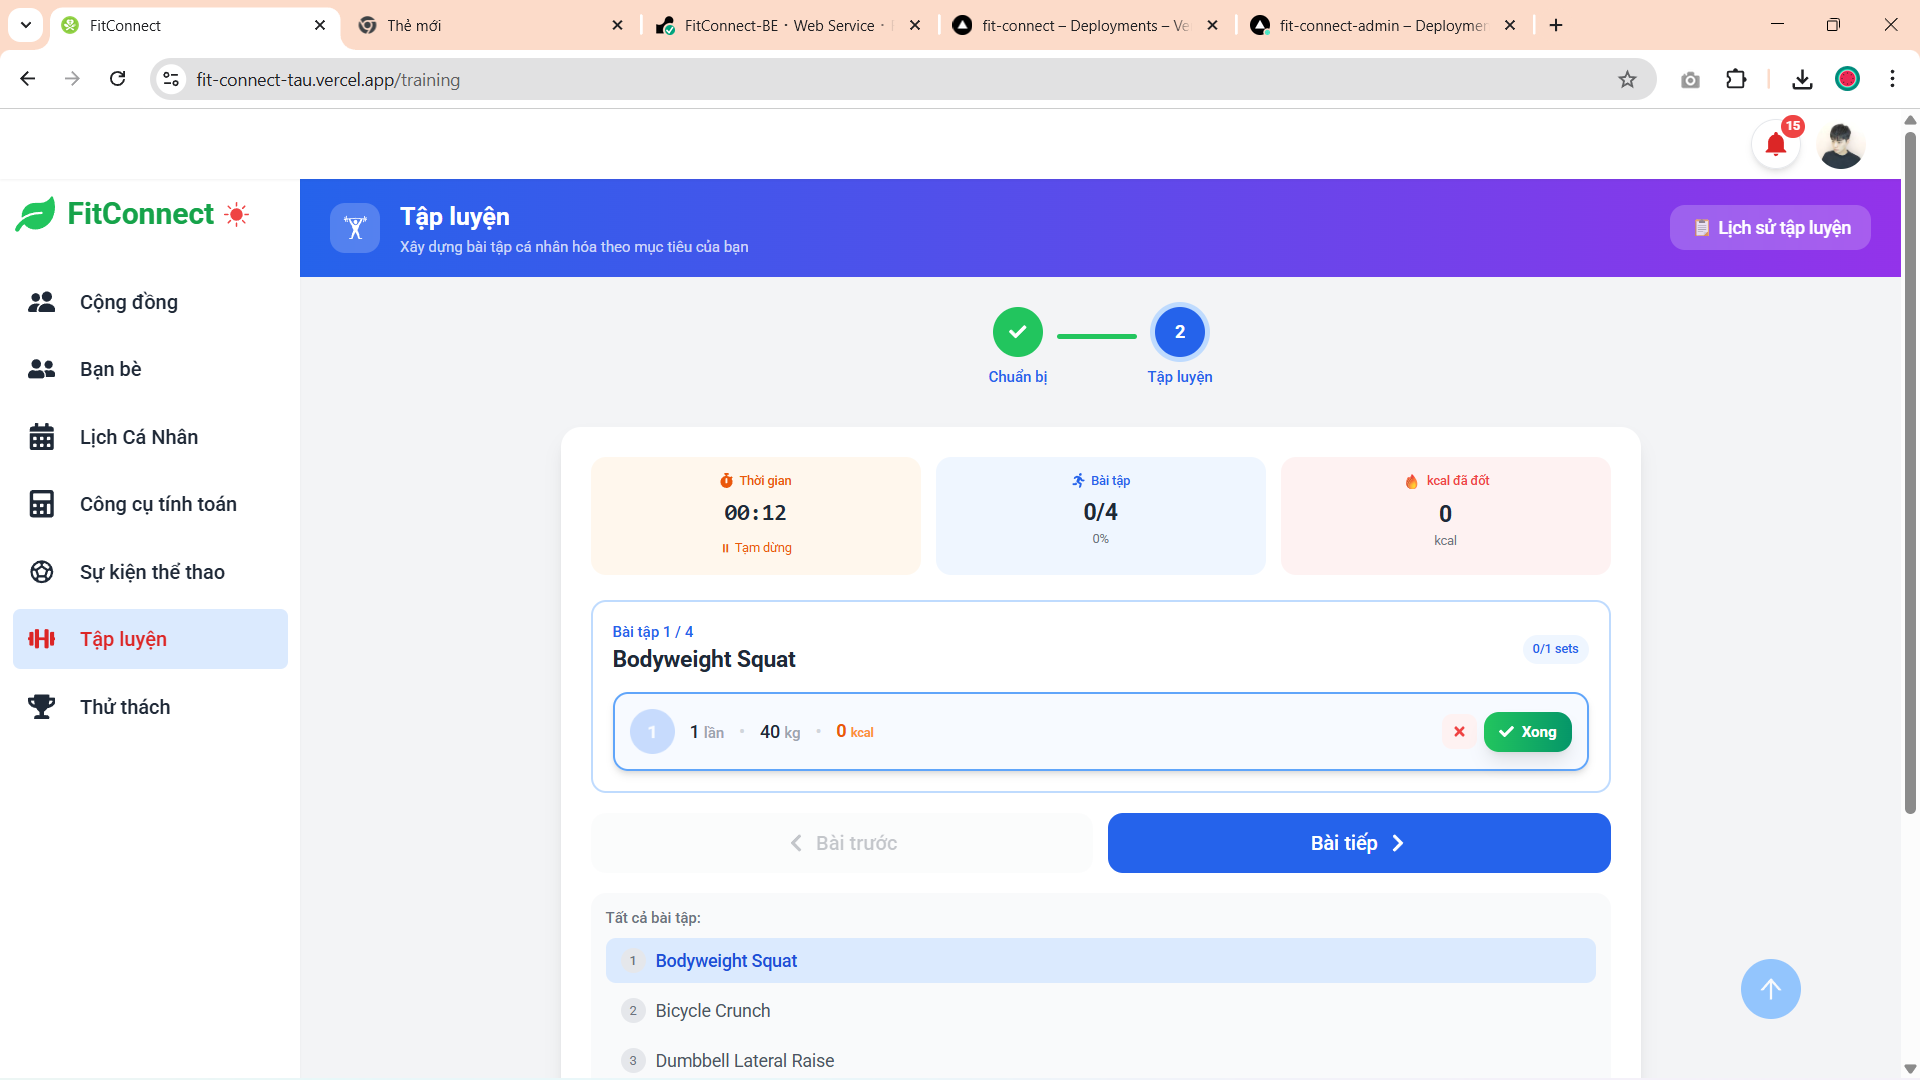
\includegraphics[width=0.60\textwidth]{Images/IMG/nhom6/batdautapluyen.png}
    \caption{Người dùng thực hiện tập luyện và theo dõi tiến độ từng bài tập}
    \label{fig:impl_calc_training}
\end{figure}


    \item Sau khi hoàn thành tất cả bài tập, hệ thống đánh dấu xanh toàn bộ danh sách và hiện nút ``Hoàn thành tập luyện''. Khi xác nhận, buổi tập được ghi nhận tự động vào lịch sử tập luyện của người dùng.

\end{itemize}

\subsubsection{Theo dõi lịch sử chỉ số sức khỏe}

\begin{itemize}
    \item Người dùng chuyển sang tab ``Lịch sử chỉ số''. Hệ thống hiển thị tổng quan các chỉ số sức khỏe hiện tại (BMI, BMR, TDEE, Body Fat, LBM, IBW) dưới dạng thẻ tóm tắt ở đầu trang. Bên dưới, hệ thống hiển thị biểu đồ theo dõi theo thời gian cho từng chỉ số: Cân nặng (kg), BMI (kg/m²), BMR (kcal), TDEE (kcal/ngày), Body Fat (\%), LBM (kg) và IBW (kg). Mỗi biểu đồ có nút ``Cập nhật'' để người dùng cập nhật chỉ số mới nhất.

    \item Người dùng có thể lọc dữ liệu biểu đồ theo các khoảng thời gian: 1 ngày, 7 ngày, 1 tháng, 6 tháng, Tất cả, hoặc Tùy chọn (chọn ngày cụ thể). Hệ thống cũng hiển thị phần ``Chỉ số chưa có'' kèm nút tính nhanh để người dùng bổ sung các chỉ số còn thiếu.

\begin{figure}[H]
    \centering
    
\includegraphics[width=0.60\textwidth]{Images/IMG/nhom6/lichsuchiso.png}
    \caption{Hệ thống hiển thị lịch sử chỉ số sức khỏe với biểu đồ theo thời gian}
    \label{fig:impl_calc_history}
\end{figure}

\end{itemize}

\subsection{Nhóm tính năng Tập luyện}
\label{subsec:impl_training}

Nhóm tính năng Tập luyện là hệ sinh thái xây dựng và thực hiện bài tập cá nhân hóa theo mục tiêu sức khỏe của người dùng. Hệ thống cung cấp 4 chế độ luyện tập đa dạng: \textbf{Tùy chỉnh} (tự chọn thiết bị, nhóm cơ, bài tập), \textbf{AI Gợi ý Tập Luyện} (mô tả tình trạng sức khỏe để AI phân tích và gợi ý bài tập phù hợp), \textbf{Hoạt động ngoài trời} (chạy bộ, đạp xe với theo dõi GPS thời gian thực trên bản đồ), và \textbf{Bài tập đã lưu} (sử dụng lại giáo án đã lưu kèm lịch tập định kỳ). Ngoài ra, hệ thống tích hợp trang Lịch sử tập luyện giúp người dùng theo dõi toàn bộ hoạt động tập luyện theo thời gian.

\subsubsection{Luồng tập luyện Tùy chỉnh}

\begin{itemize}
    \item Người dùng truy cập trang Tập luyện từ thanh điều hướng bên trái. Hệ thống hiển thị giao diện ``Chọn chế độ luyện tập'' với 4 thẻ chế độ: Tùy chỉnh (tự chọn thiết bị, nhóm cơ và bài tập theo ý muốn), AI Gợi ý Tập Luyện (mô tả tình trạng sức khỏe để AI tư vấn và gợi ý bài tập phù hợp), Hoạt động ngoài trời (chạy bộ, đạp xe, ghi hoạt động theo thời gian thực trên bản đồ), và Bài tập đã lưu (sử dụng lại giáo án đã lưu trước đó). Ở góc trên bên phải, hệ thống hiển thị nút ``Lịch sử tập luyện'' để truy cập nhanh lịch sử.

\begin{figure}[H]
    \centering
    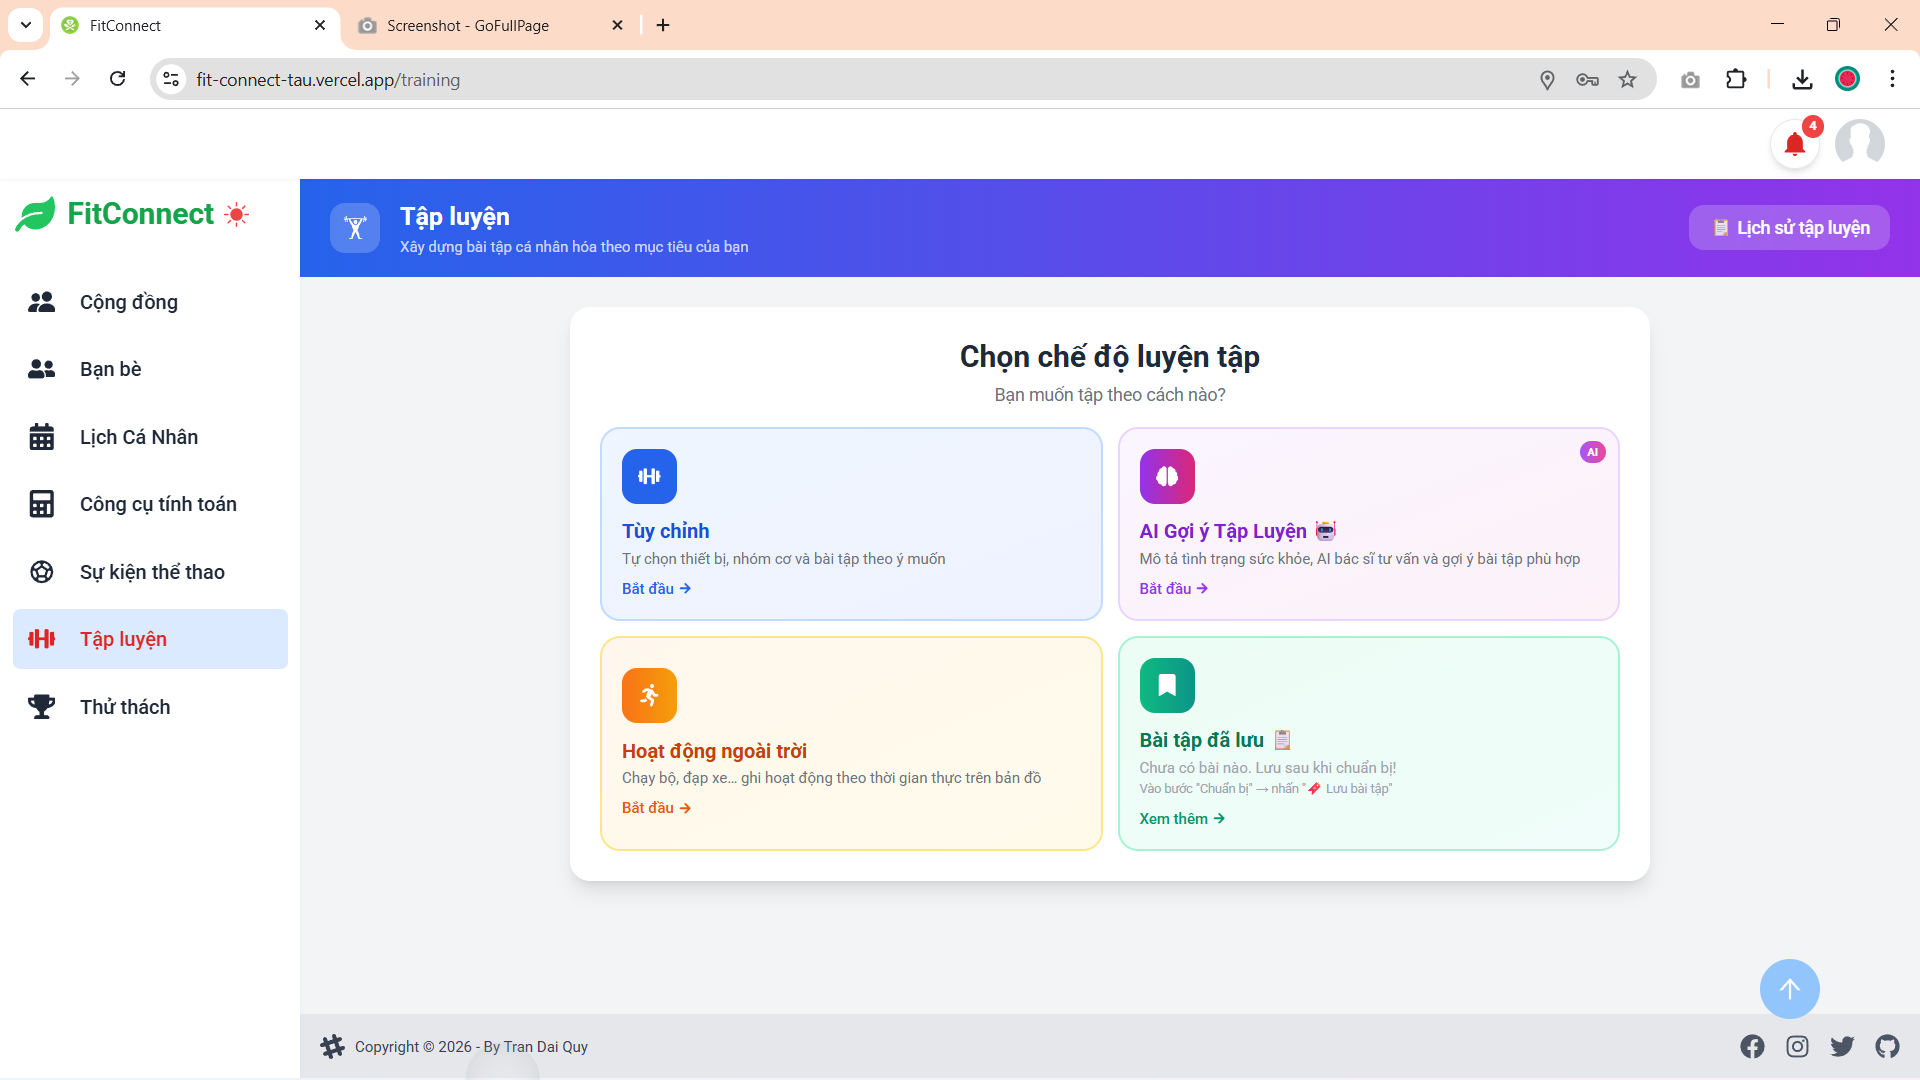
\includegraphics[width=0.60\textwidth]{Images/IMG/nhom5/manhinhtapluyen.png}
    \caption{Hệ thống hiển thị trang Tập luyện với 4 chế độ luyện tập}
    \label{fig:impl_train_main}
\end{figure}


    \item Khi chọn chế độ ``Tùy chỉnh'', hệ thống bắt đầu quy trình 5 bước. \textbf{Bước 1 -- Thiết bị}: Hệ thống hiển thị giao diện ``Chọn thiết bị của bạn'' với 8 loại thiết bị tập: Cơ thể (không cần thiết bị), Dây kháng lực (Resistance Band / Cable), Ghế tập (Bench), Máy / Đĩa tạ (Machine / Plate), Tạ tay (Dumbbell), Tạ đòn (Barbell), Tạ ấm (Kettlebell), và Xà đơn (Pull-up bar). Người dùng chọn các thiết bị có sẵn và nhấn ``Tiếp tục''.

\begin{figure}[H]
    \centering
    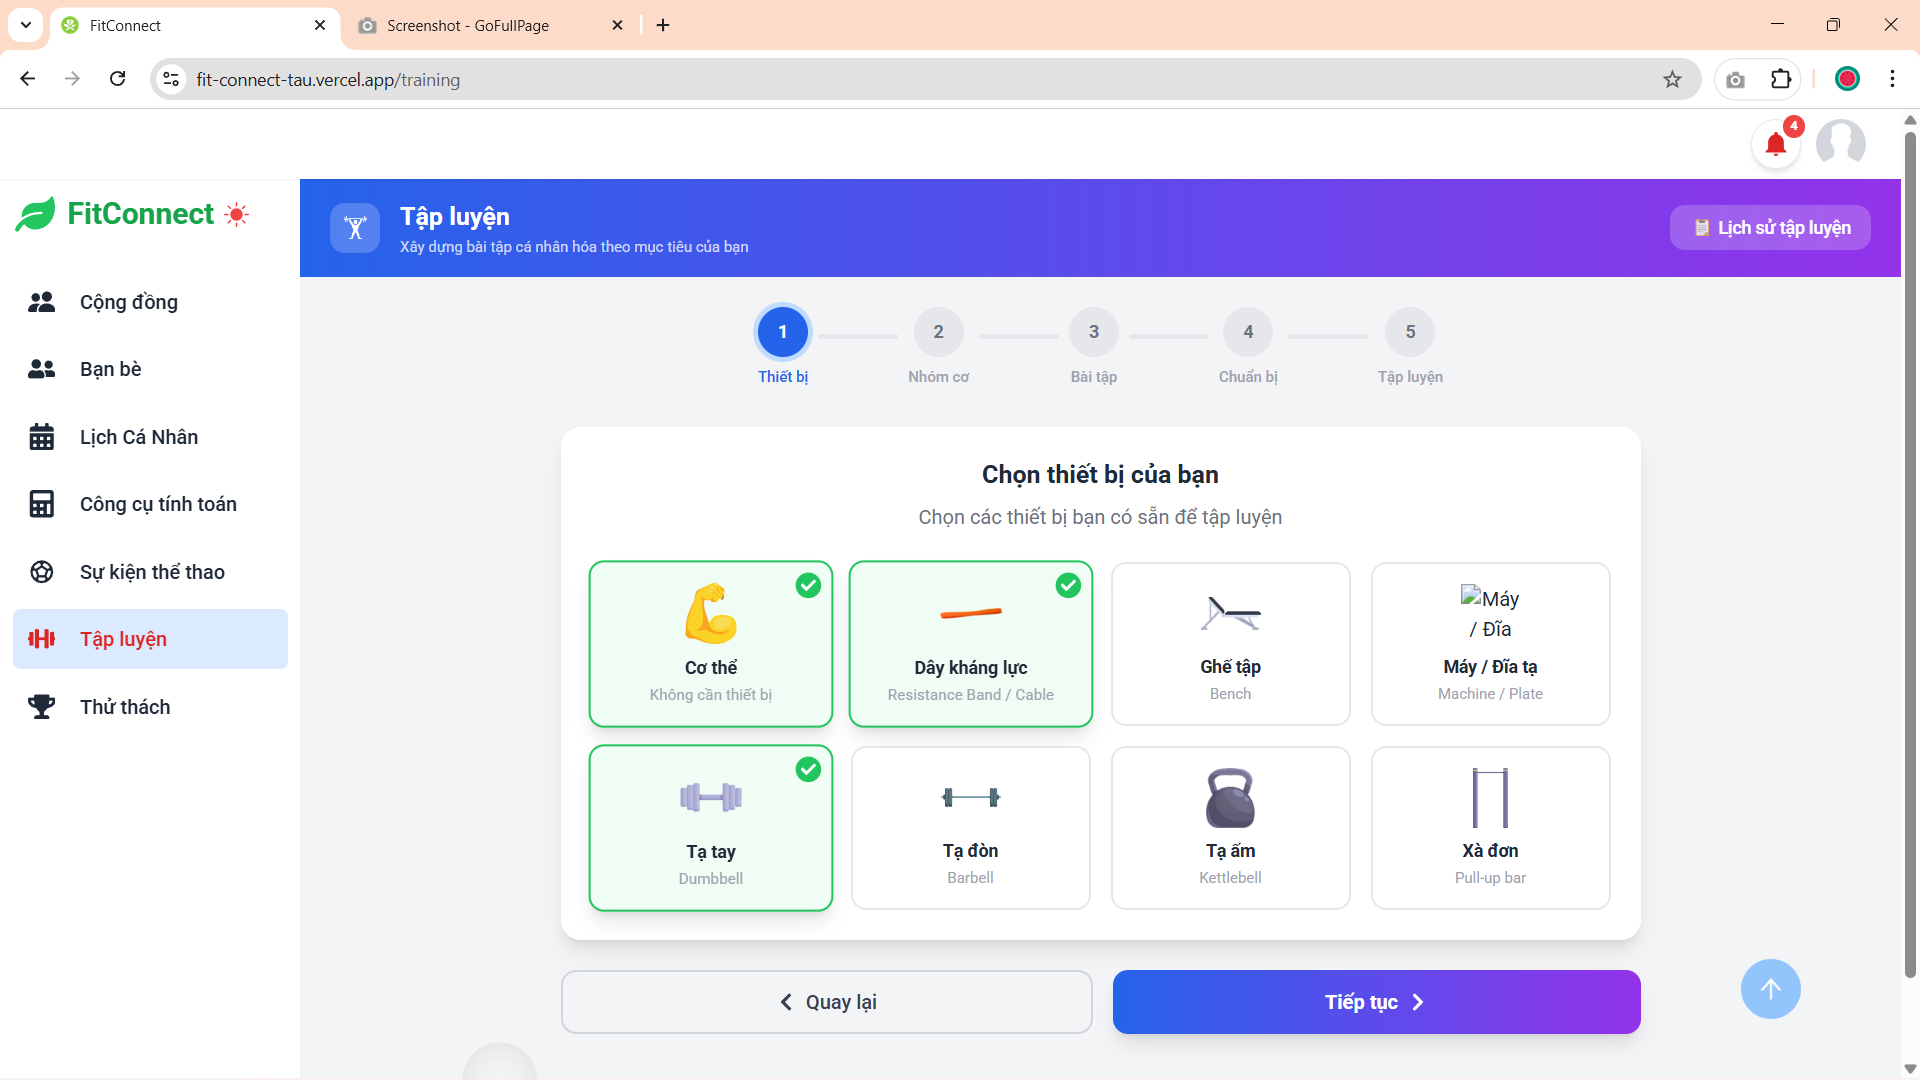
\includegraphics[width=0.60\textwidth]{Images/IMG/nhom5/chonthietbitap.png}
    \caption{Người dùng chọn thiết bị tập luyện có sẵn tại Bước 1}
    \label{fig:impl_train_equipment}
\end{figure}


    \item \textbf{Bước 2 -- Nhóm cơ}: Hệ thống hiển thị mô hình cơ thể người tương tác (mặt trước và mặt sau). Người dùng nhấn trực tiếp vào các vùng cơ trên mô hình để chọn nhóm cơ muốn tập (ví dụ: Vai trước, Bắp tay trước, Cẳng tay, Chéo bụng, Bụng, Ngực, Đùi trước,...). Các vùng cơ được chọn sẽ sáng lên màu xanh trên mô hình và hiển thị dưới dạng tag ở phía trên. Nhấn ``Tiếp tục'' để chuyển bước.

\begin{figure}[H]
    \centering
    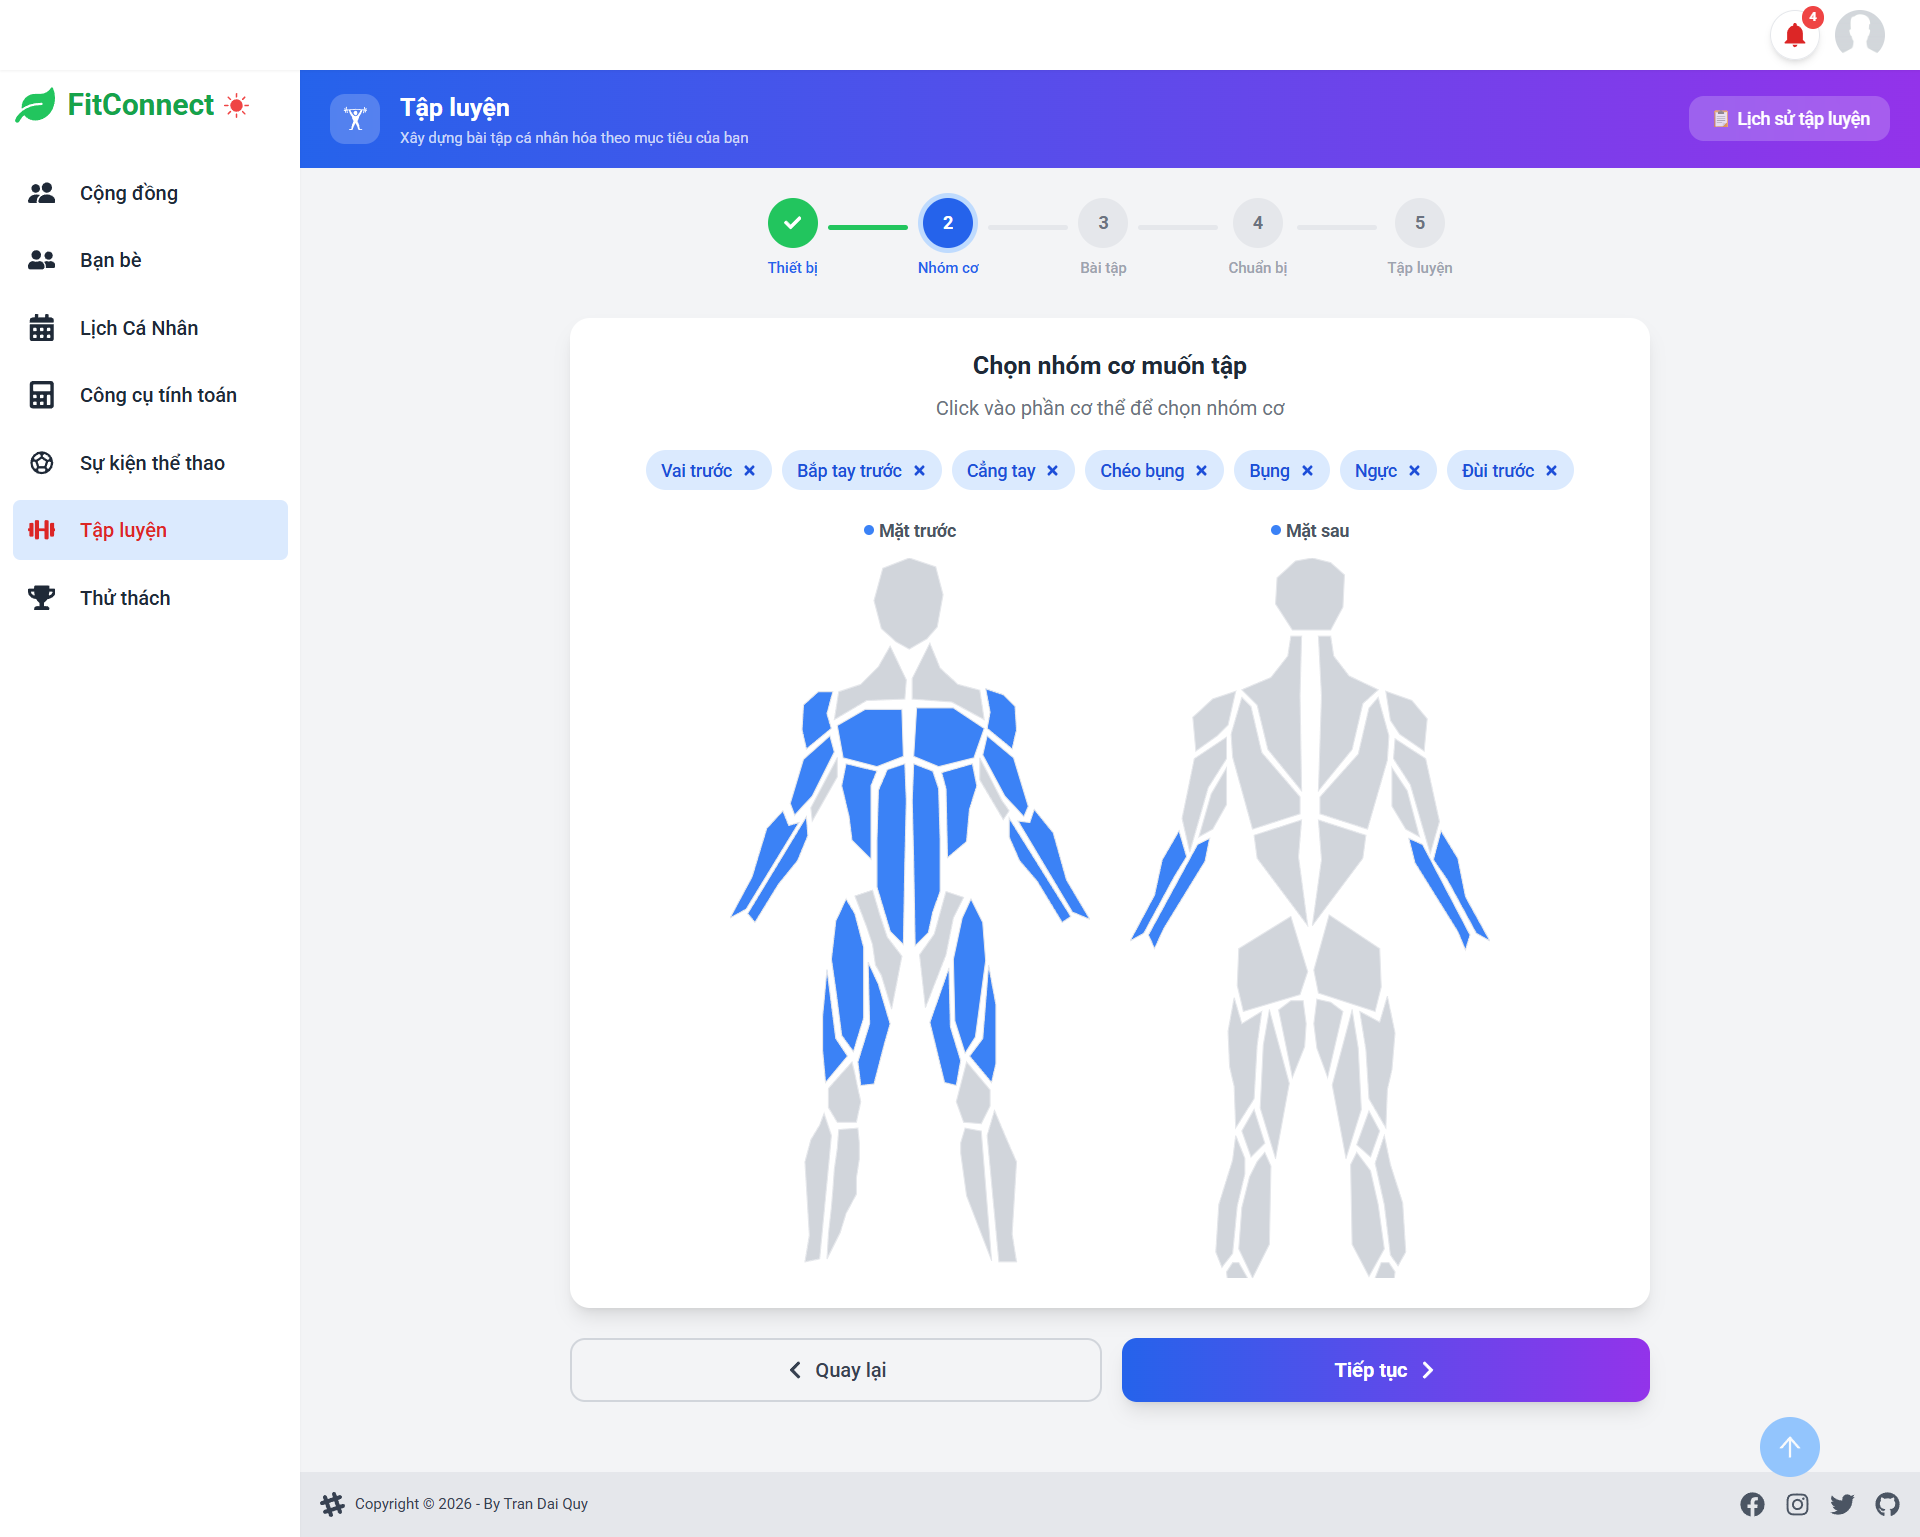
\includegraphics[width=0.60\textwidth]{Images/IMG/nhom5/chonnhomco.png}
    \caption{Người dùng chọn nhóm cơ muốn tập trên mô hình cơ thể tương tác tại Bước 2}
    \label{fig:impl_train_muscle}
\end{figure}


    \item \textbf{Bước 3 -- Bài tập}: Hệ thống lọc và hiển thị danh sách bài tập phù hợp với thiết bị và nhóm cơ đã chọn. Mỗi bài tập hiển thị: tên tiếng Anh, tên tiếng Việt, mức độ (Dễ, Trung bình), số set và reps mặc định. Phần ``Đã chọn'' ở trên cho phép kéo thả để sắp xếp lại thứ tự. Người dùng nhấn vào biểu tượng thông tin để xem chi tiết bài tập.

\begin{figure}[H]
    \centering
    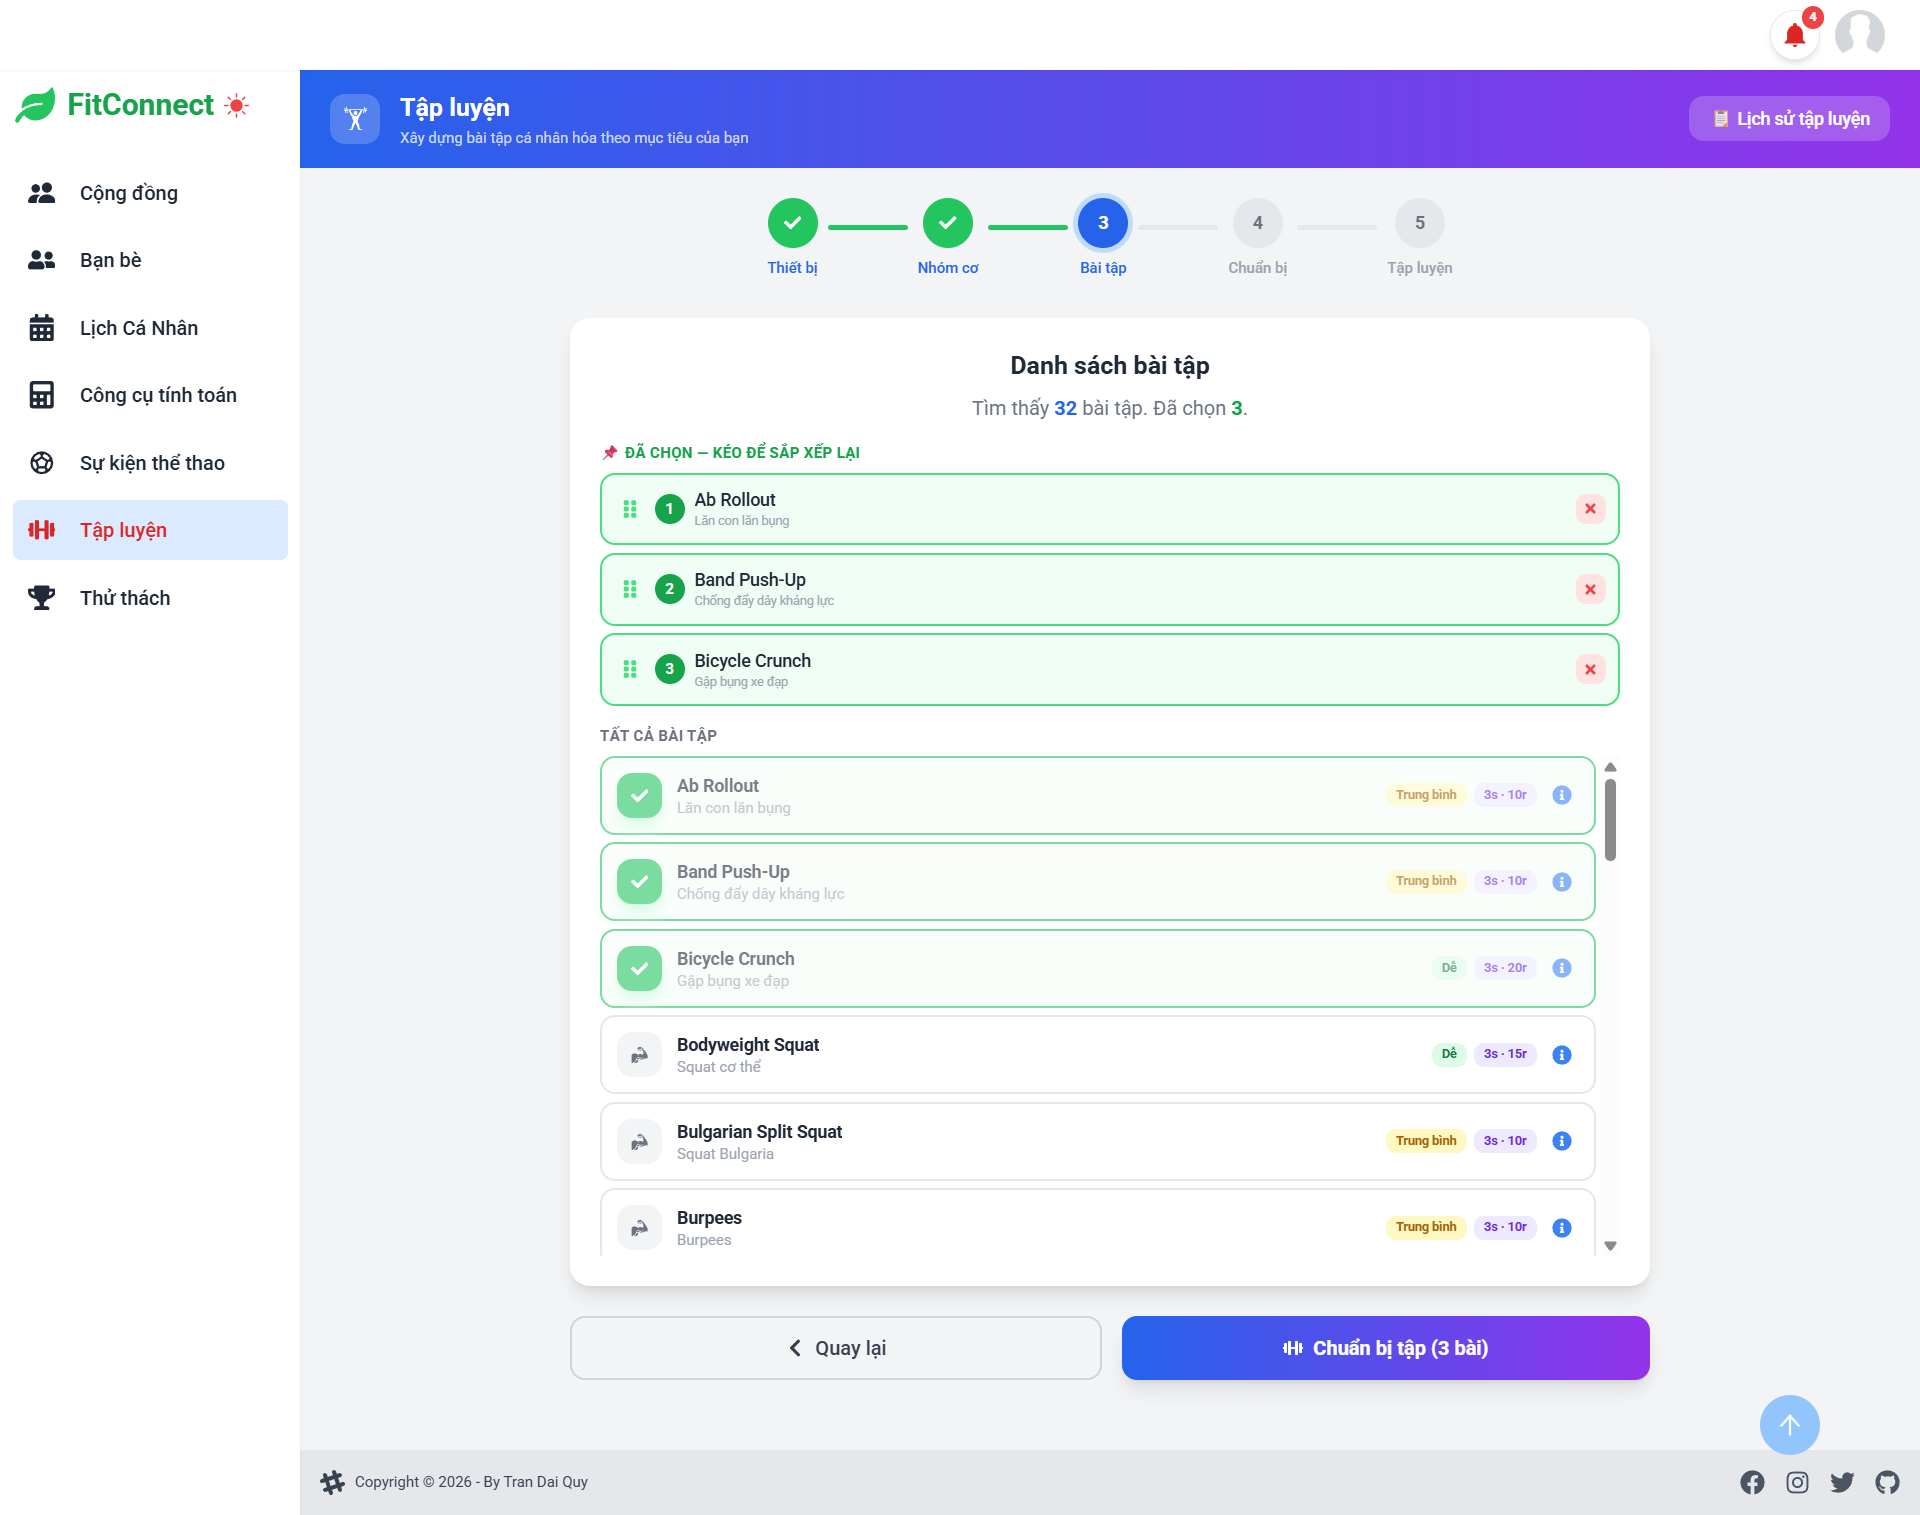
\includegraphics[width=0.60\textwidth]{Images/IMG/nhom5/chonbaitap.png}
    \caption{Người dùng chọn bài tập từ danh sách được lọc theo thiết bị và nhóm cơ tại Bước 3}
    \label{fig:impl_train_exercises}
\end{figure}


    \item Khi nhấn biểu tượng thông tin của một bài tập, hệ thống hiển thị modal chi tiết gồm: video hướng dẫn từ YouTube, tên bài tập (tiếng Anh và tiếng Việt), nhãn mức độ (Dễ), loại bài tập (Sức mạnh), lượng kcal/đơn vị, phần ``Hướng dẫn thực hiện'' với các bước chi tiết đánh số, và phần ``Mẹo'' với lời khuyên kỹ thuật.

\begin{figure}[H]
    \centering
    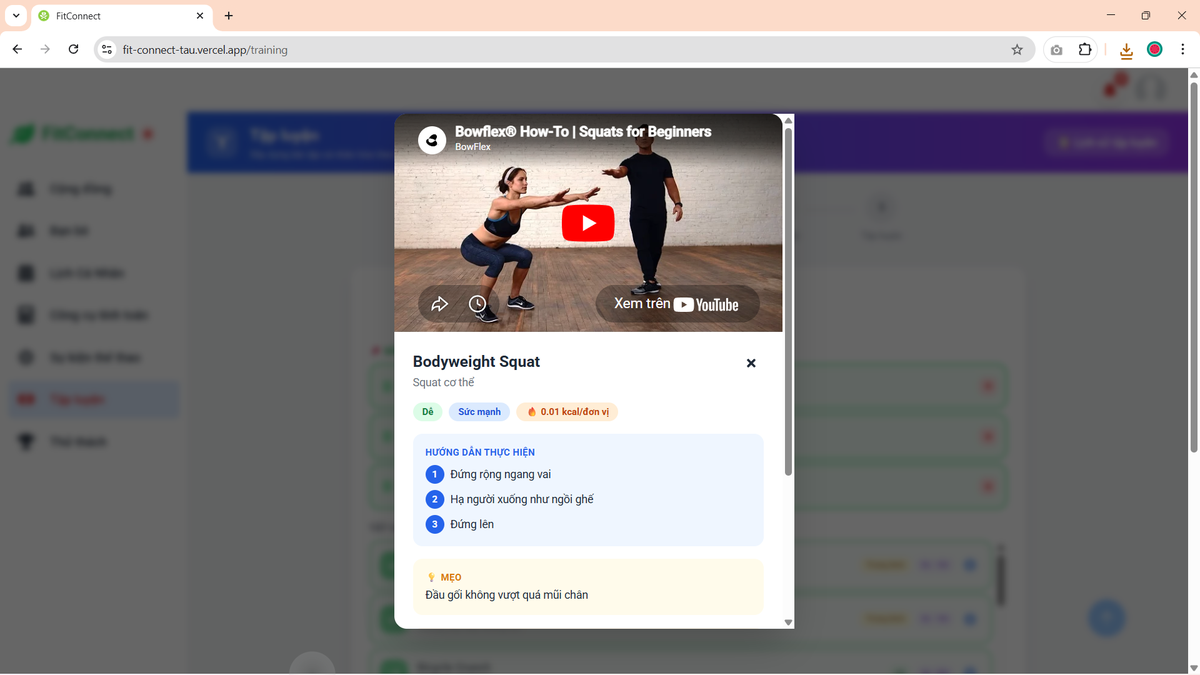
\includegraphics[width=0.60\textwidth]{Images/IMG/nhom5/xemthongtinbaitap.png}
    \caption{Hệ thống hiển thị thông tin chi tiết bài tập kèm video hướng dẫn}
    \label{fig:impl_train_detail}
\end{figure}


    \item \textbf{Bước 4 -- Chuẩn bị}: Sau khi chọn bài tập và nhấn ``Chuẩn bị tập'', hệ thống hiển thị trang Chuẩn bị tập luyện với tổng quan (số bài tập, tổng sets). Mỗi bài tập hiển thị bảng chi tiết gồm: SET, Reps (Số lần), Weight (Mức tạ -- kg), và kcal tự động tính. Người dùng có thể chỉnh sửa số lần, mức tạ, thêm set (nút ``+ Thêm set''), hoặc xóa set. Hệ thống hiển thị tổng kcal ước tính. Tại đây, người dùng có 3 lựa chọn: ``Quay lại'', ``Lưu bài tập'' (lưu giáo án cho lần sau), hoặc ``Bắt đầu tập!'' để bắt đầu tập luyện.

\begin{figure}[H]
    \centering
    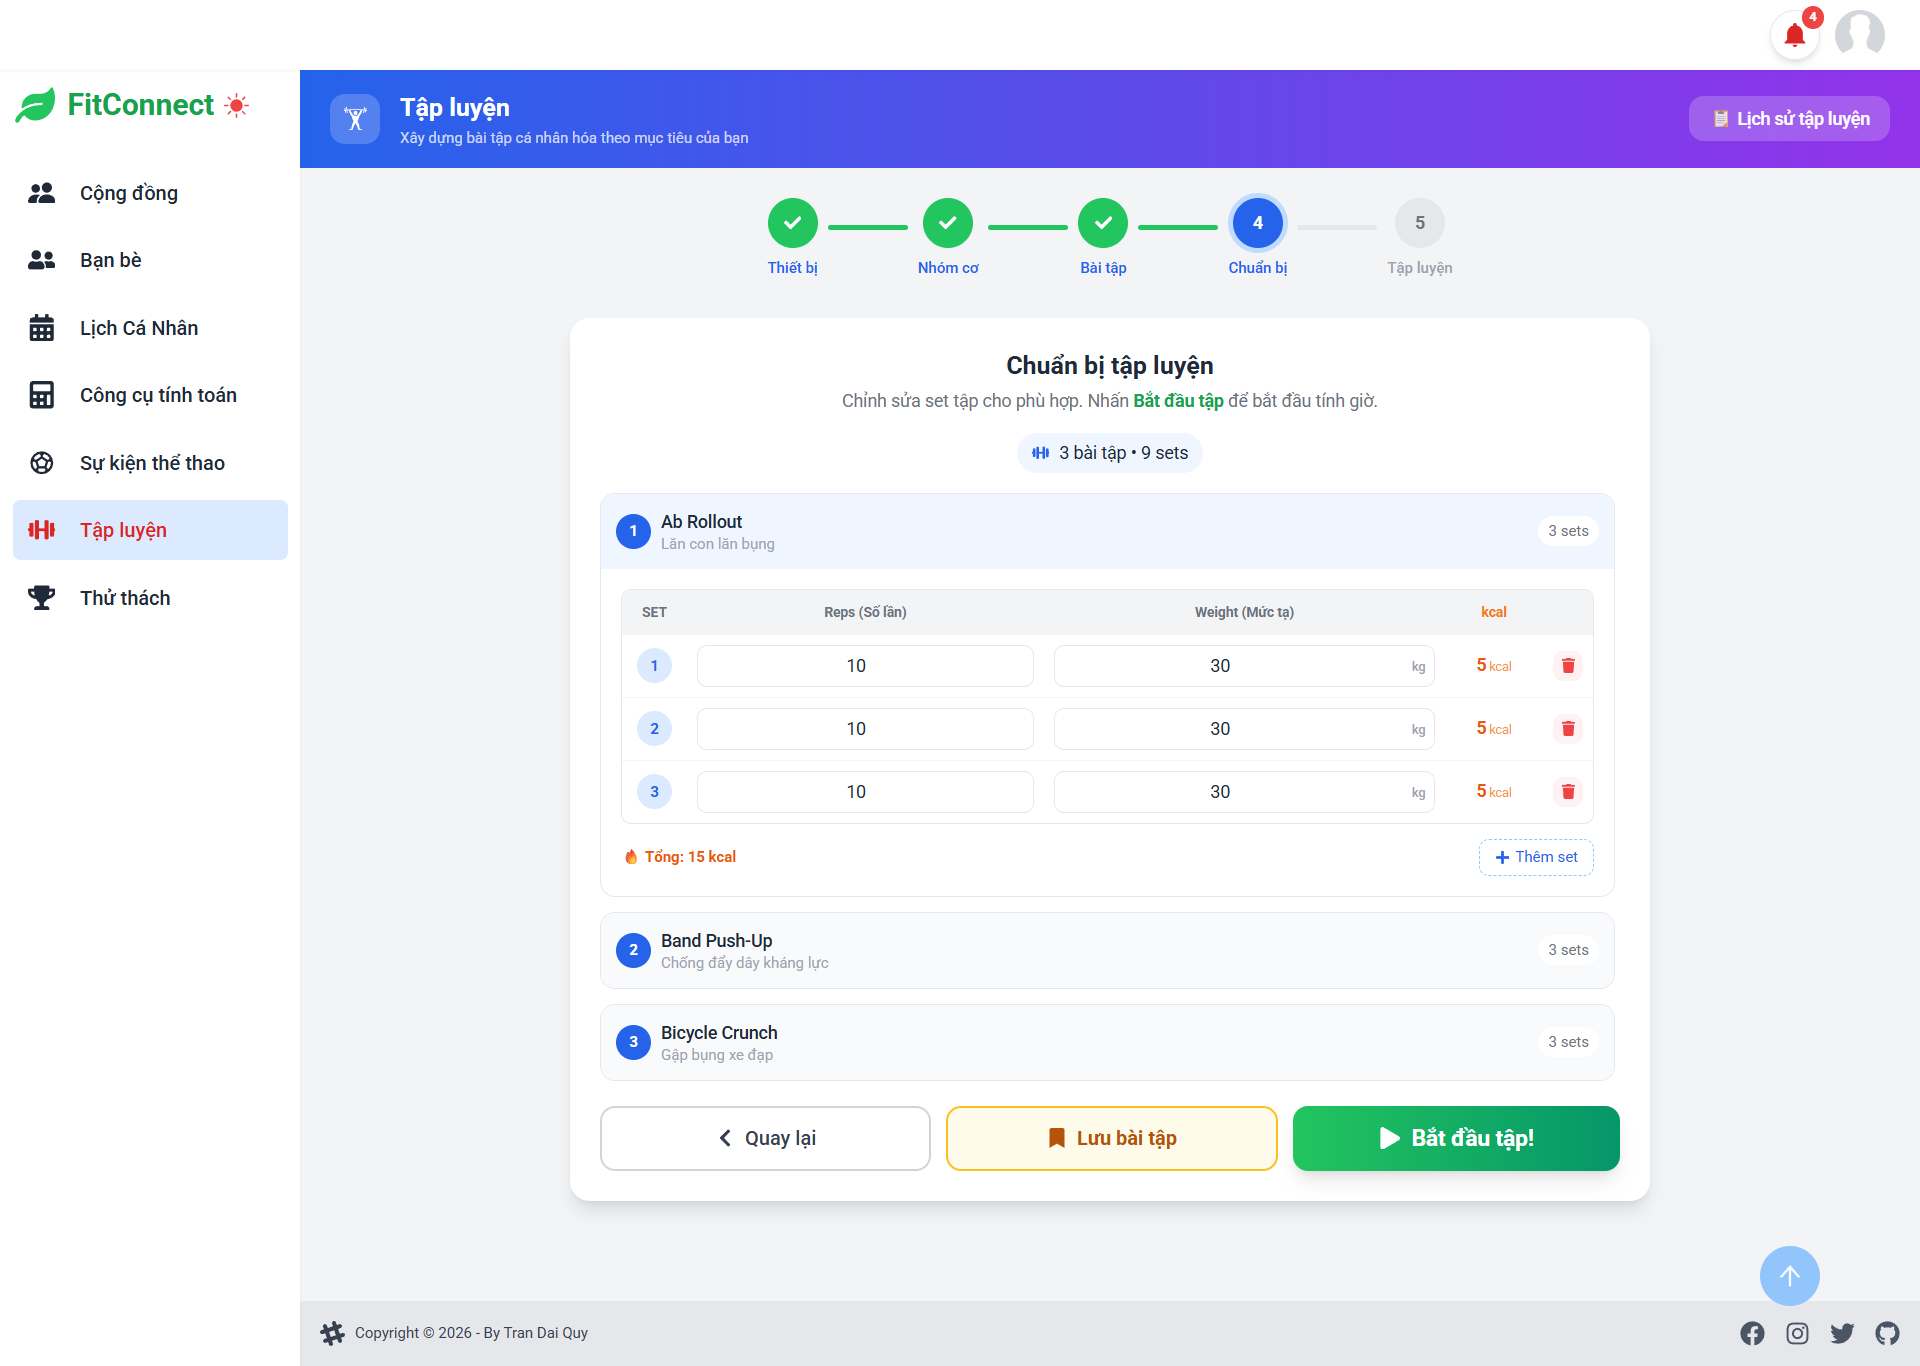
\includegraphics[width=0.60\textwidth]{Images/IMG/nhom5/buocchuanbitapluyen.png}
    \caption{Người dùng cấu hình sets, reps, mức tạ cho từng bài tập tại Bước 4 -- Chuẩn bị}
    \label{fig:impl_train_prep}
\end{figure}


    \item \textbf{Bước 5 -- Tập luyện}: Khi nhấn ``Bắt đầu tập!'', hệ thống chuyển sang trang Tập luyện hiển thị 3 thông số theo dõi thời gian thực: Thời gian (đồng hồ đếm), Bài tập (số bài hoàn thành/tổng, phần trăm), và kcal đã đốt. Mỗi bài tập hiển thị từng set với thông tin (số lần, mức tạ, kcal). Người dùng nhấn ``Xong'' cho từng set sau khi hoàn thành, sau đó nhấn ``Bài tiếp'' để chuyển sang bài tập kế tiếp. Phần ``Tất cả bài tập'' ở dưới hiển thị tiến độ tổng thể với đánh dấu xanh cho các bài đã hoàn thành. Người dùng cũng có thể nhấn ``Bỏ tập'' nếu muốn hủy buổi tập.

\begin{figure}[H]
    \centering
    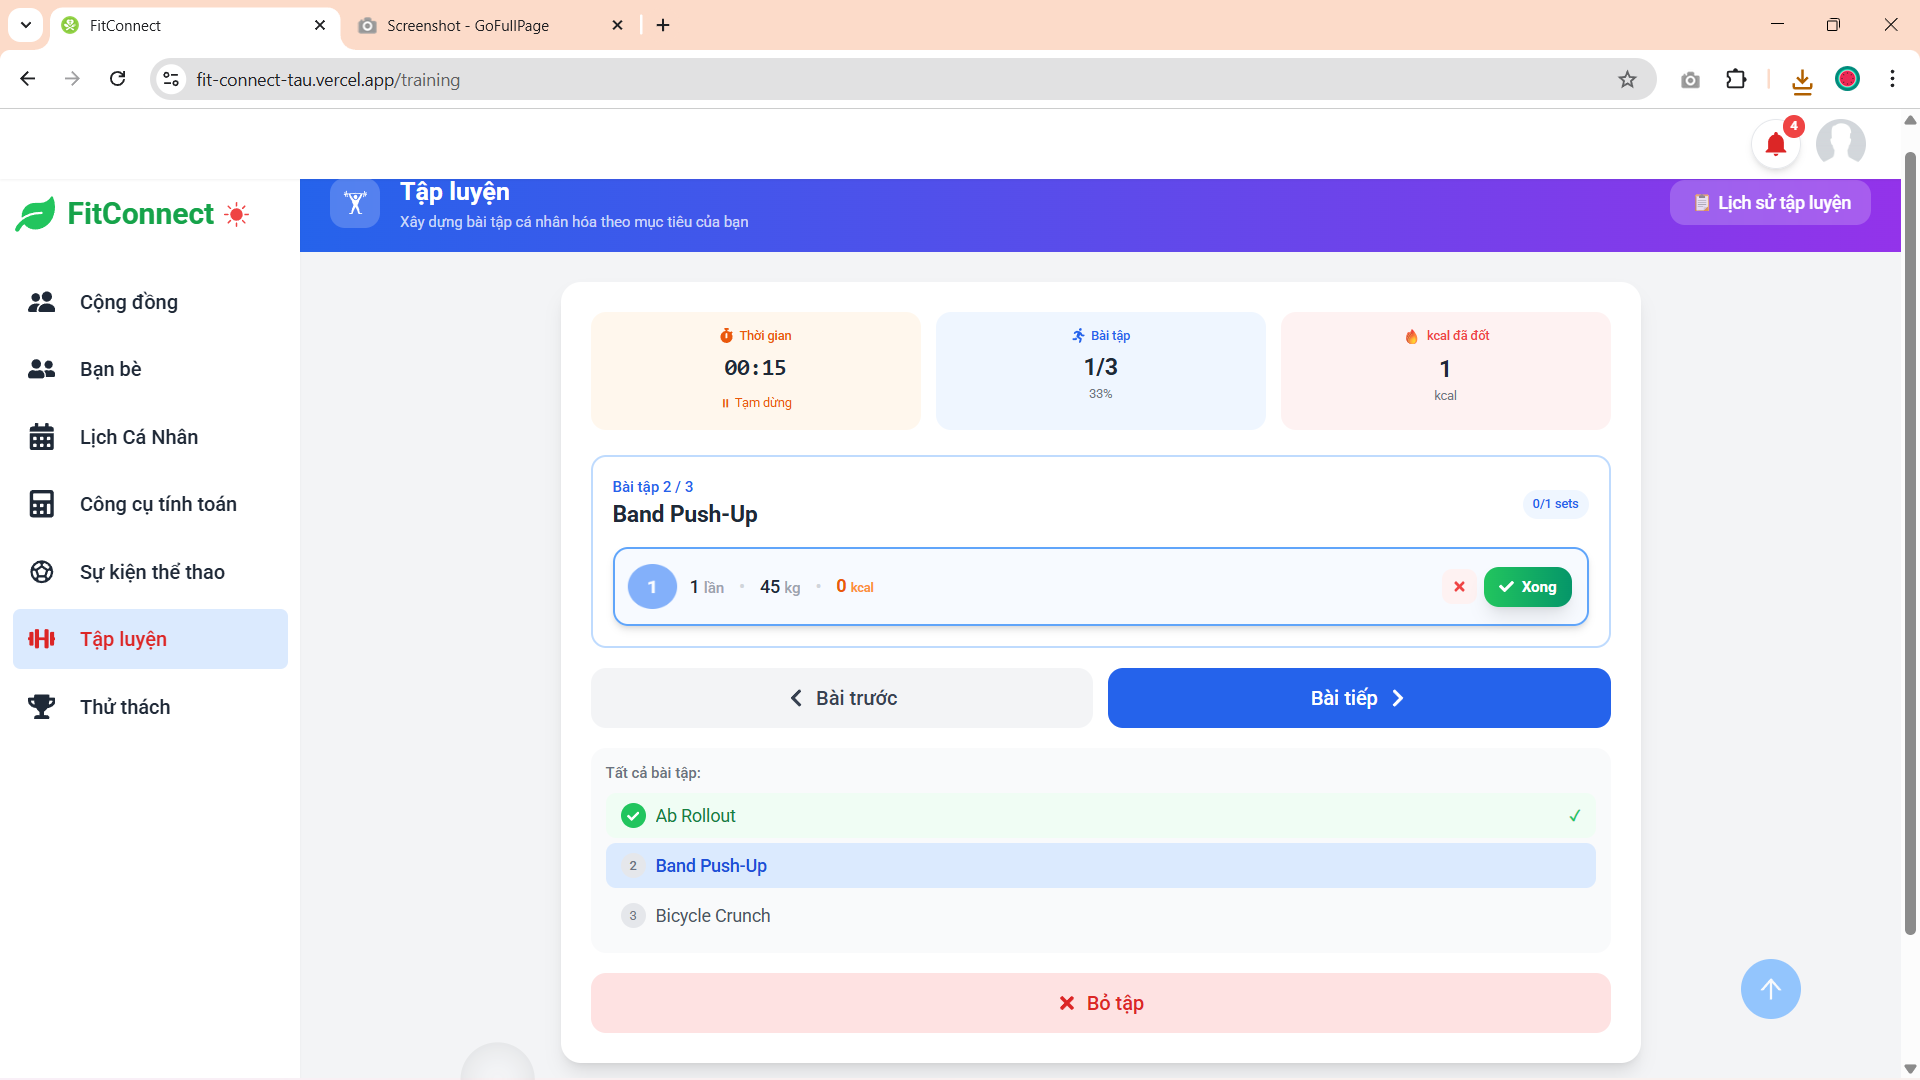
\includegraphics[width=0.60\textwidth]{Images/IMG/nhom5/tabbatdautapluyen.png}
    \caption{Người dùng thực hiện tập luyện và theo dõi tiến độ từng set tại Bước 5}
    \label{fig:impl_train_active}
\end{figure}


    \item Sau khi hoàn thành tất cả bài tập, hệ thống hiển thị trạng thái 100\% và nút ``Hoàn thành tập luyện''. Khi xác nhận, buổi tập được ghi nhận tự động vào lịch sử tập luyện.

\end{itemize}

\subsubsection{Luồng tập luyện AI Gợi ý}

\begin{itemize}
    \item Khi chọn chế độ ``AI Gợi ý Tập Luyện'', hệ thống hiển thị giao diện với ô nhập liệu ``Mô tả tình trạng và mục tiêu tập luyện''. Người dùng nhập mô tả tình trạng sức khỏe hiện tại bằng ngôn ngữ tự nhiên (ví dụ: ``Tôi bị đau lưng, cho tôi các bài viết nhẹ nhàng'') và nhấn nút ``Phân tích AI''.

\begin{figure}[H]
    \centering
    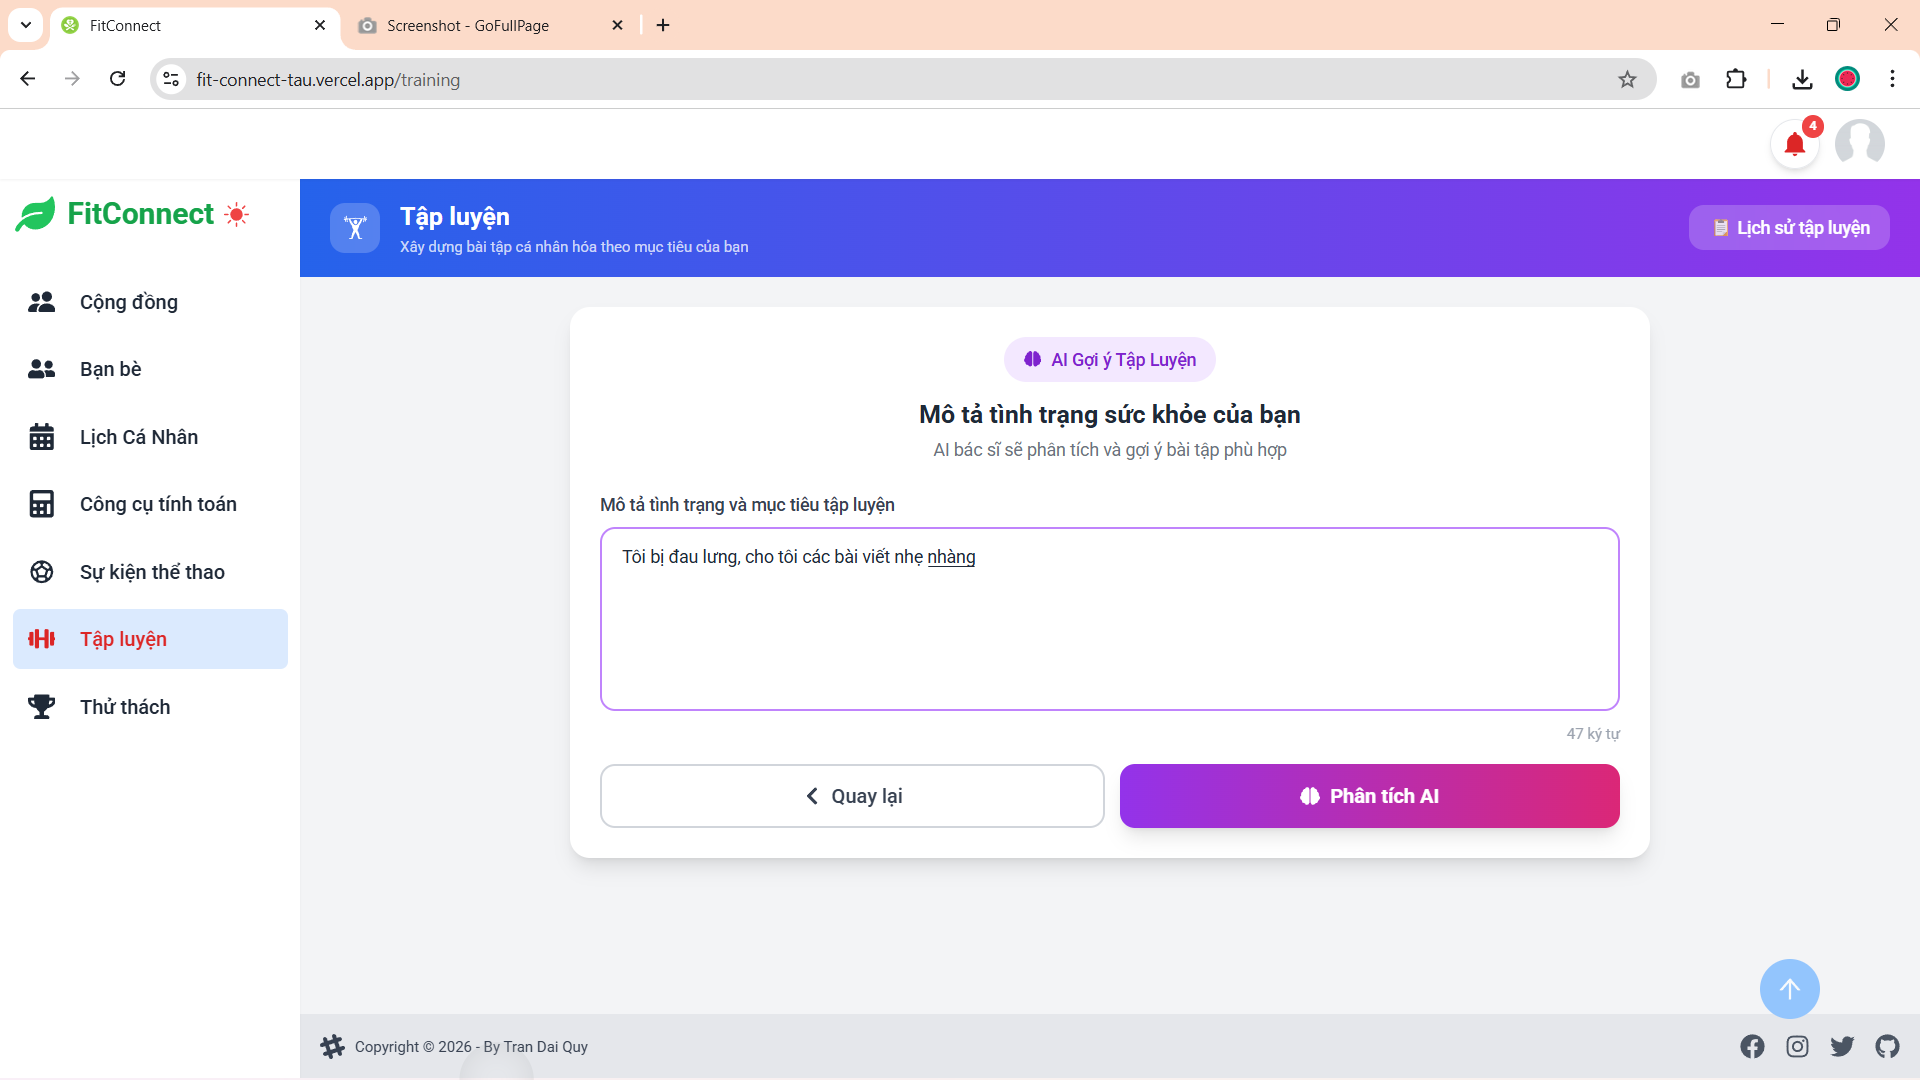
\includegraphics[width=0.60\textwidth]{Images/IMG/nhom5/manhinhAIgoiybaitap.png}
    \caption{Người dùng nhập mô tả tình trạng sức khỏe để AI phân tích và gợi ý bài tập}
    \label{fig:impl_train_ai_input}
\end{figure}


    \item Hệ thống gửi mô tả tới AI, AI phân tích và trả về kết quả gồm: phần ``Đánh giá sức khỏe từ bác sĩ'' với nhận xét chi tiết về tình trạng sức khỏe và khuyến nghị, và phần ``Bài tập gợi ý'' với danh sách bài tập phù hợp. Mỗi bài tập hiển thị: tên, nhãn mức độ (Dễ, Trung bình), loại bài tập (Sức mạnh), và lý do AI gợi ý. Người dùng chọn các bài tập muốn tập (phần ``Đã chọn'' hiển thị số lượng) và nhấn ``Bắt đầu luyện tập'' để chuyển sang trang Chuẩn bị.

\begin{figure}[H]
    \centering
    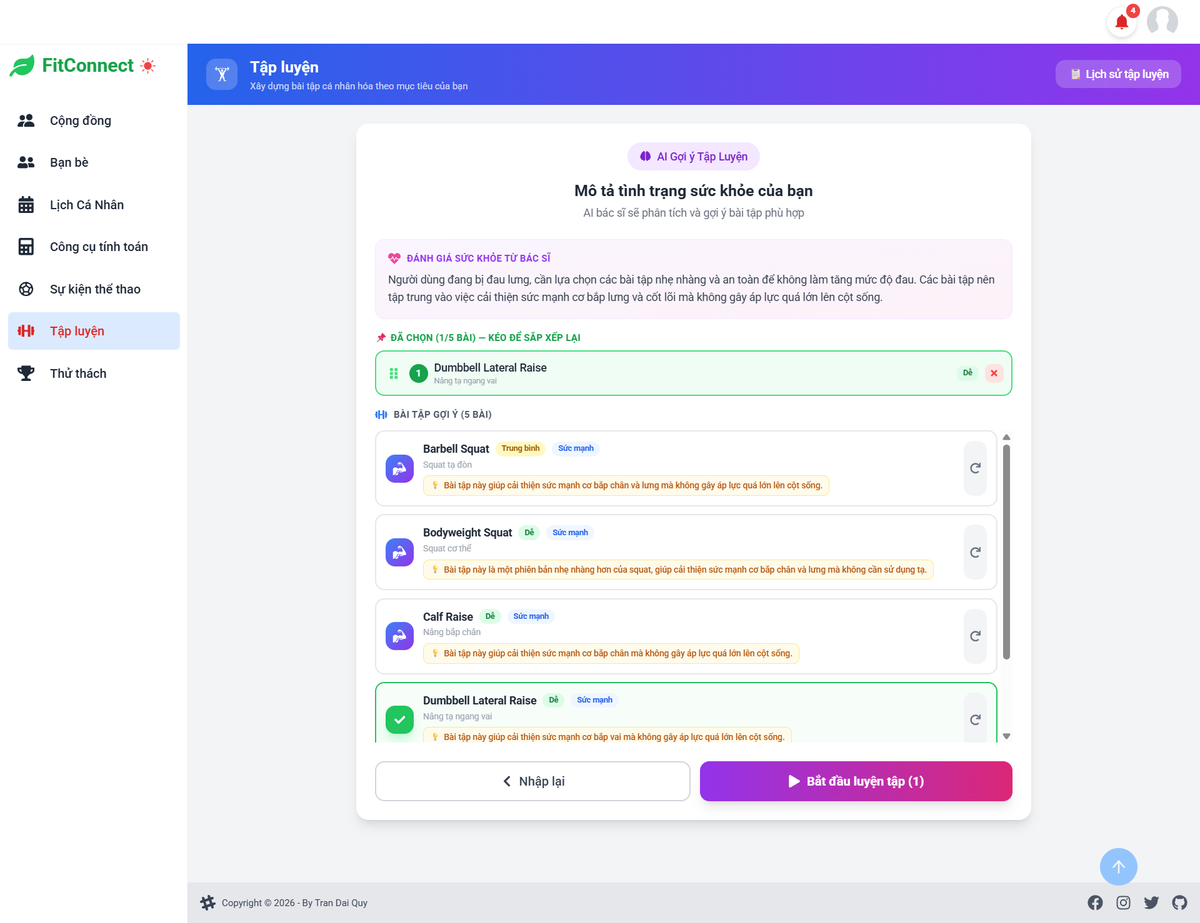
\includegraphics[width=0.60\textwidth]{Images/IMG/nhom5/aigoigoiydanhsachbaitap.png}
    \caption{Hệ thống AI phân tích sức khỏe và gợi ý danh sách bài tập phù hợp}
    \label{fig:impl_train_ai_result}
\end{figure}


    \item Sau khi chọn bài tập từ AI, hệ thống chuyển sang trang Chuẩn bị tập luyện tương tự luồng Tùy chỉnh (nhưng chỉ gồm 2 bước: Chuẩn bị và Tập luyện). Người dùng có thể chỉnh sửa sets, reps, mức tạ và bắt đầu tập luyện.

\begin{figure}[H]
    \centering
    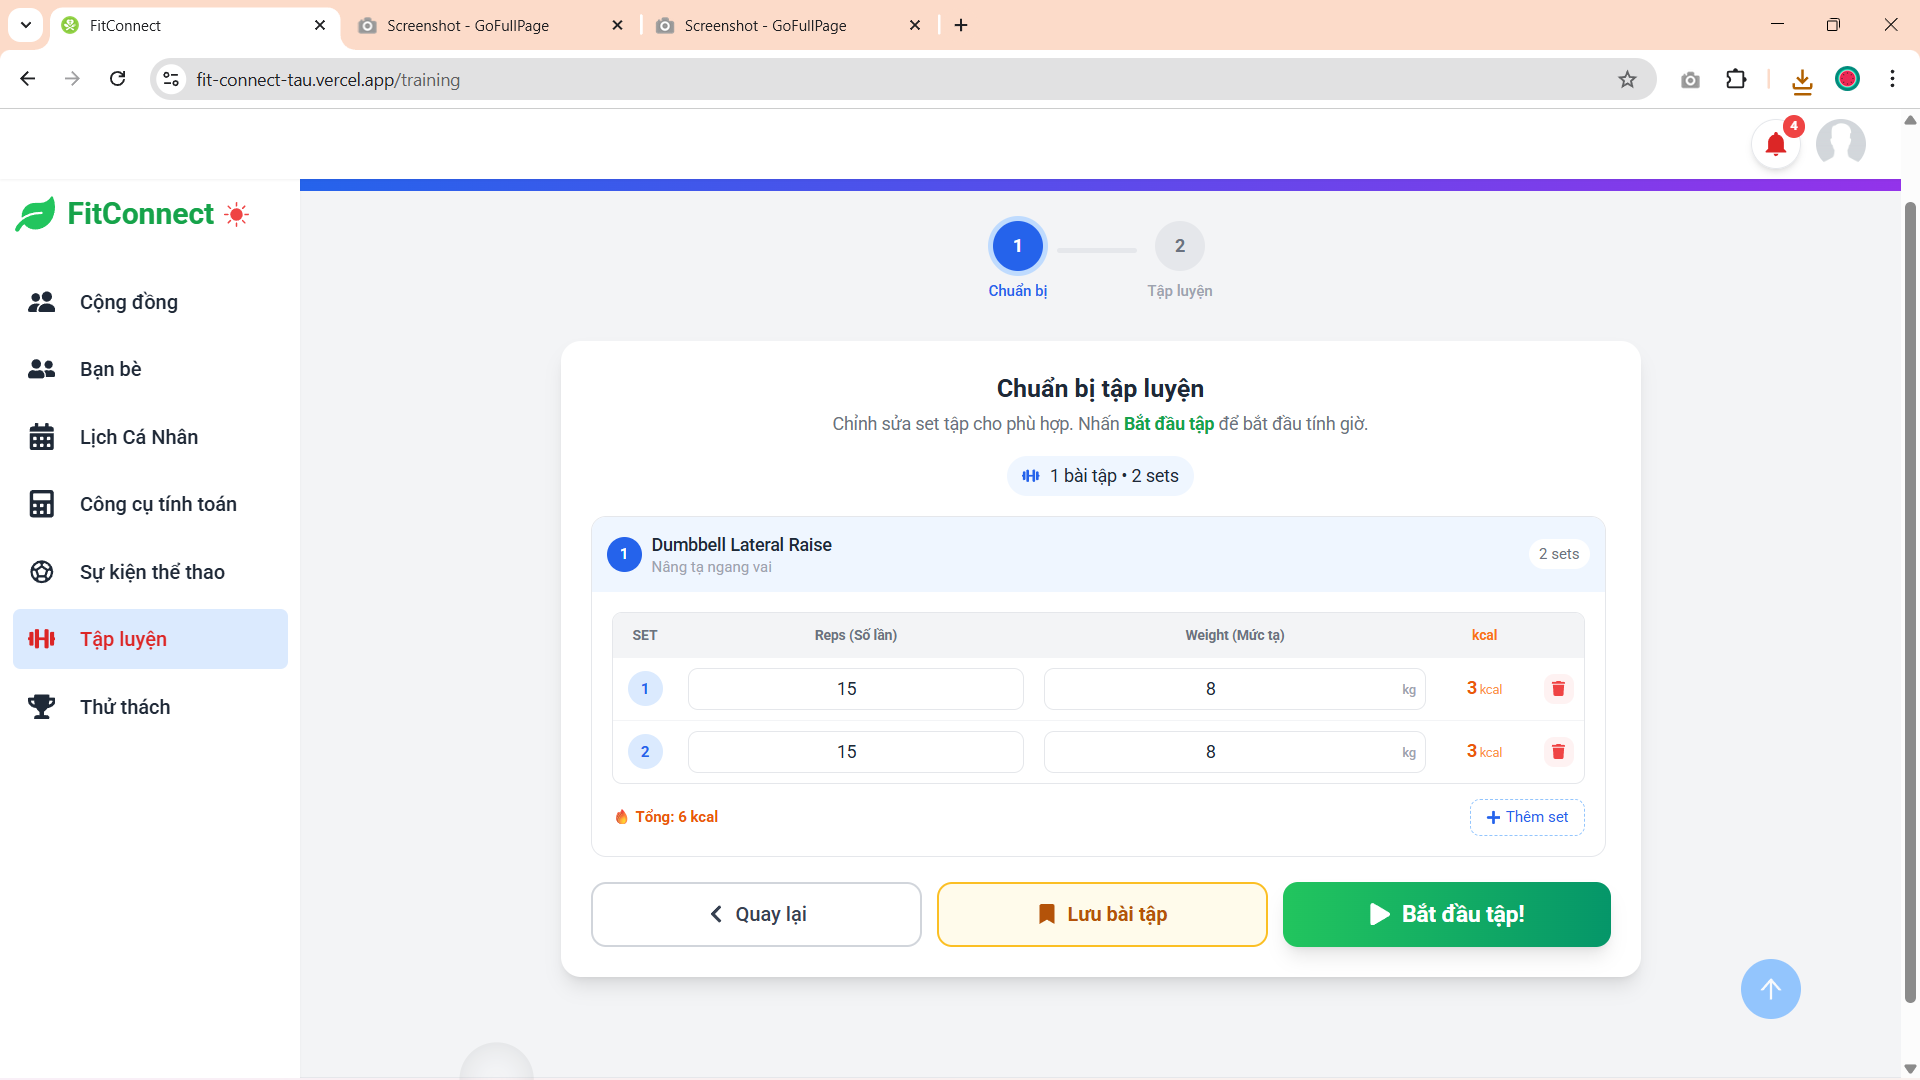
\includegraphics[width=0.60\textwidth]{Images/IMG/nhom5/manhinhchuanbitapluyentuAIqua.png}
    \caption{Người dùng chuẩn bị tập luyện với bài tập được AI gợi ý}
    \label{fig:impl_train_ai_prep}
\end{figure}

\end{itemize}

\subsubsection{Luồng Hoạt động ngoài trời}

\begin{itemize}
    \item Khi chọn chế độ ``Hoạt động ngoài trời'', hệ thống hiển thị trang thiết lập hoạt động gồm: lựa chọn môn thể thao (Chạy bộ đường dài, Đạp xe,...) kèm kcal/km ước tính, ô nhập tên bài tập, và quãng đường mục tiêu (km). Phần Tóm tắt hiển thị thông tin đã chọn. Người dùng nhấn ``Bắt đầu ghi'' để khởi động theo dõi GPS.

\begin{figure}[H]
    \centering
    
\includegraphics[width=0.60\textwidth]{Images/IMG/nhom5/tapluyenchaybo.png}
    \caption{Người dùng thiết lập hoạt động ngoài trời trước khi bắt đầu ghi GPS}
    \label{fig:impl_train_outdoor_setup}
\end{figure}


    \item Hệ thống mở giao diện GPS Tracking toàn màn hình hiển thị bản đồ thời gian thực với vị trí hiện tại. Phía dưới bản đồ, hệ thống hiển thị các thông số theo dõi: quãng đường (KM), thời gian (THỜI GIAN), tốc độ (KM/H), kcal đã đốt (KCAL), và thanh tiến trình quãng đường mục tiêu. Nút tạm dừng/tiếp tục cho phép người dùng kiểm soát buổi tập.

\begin{figure}[H]
    \centering
    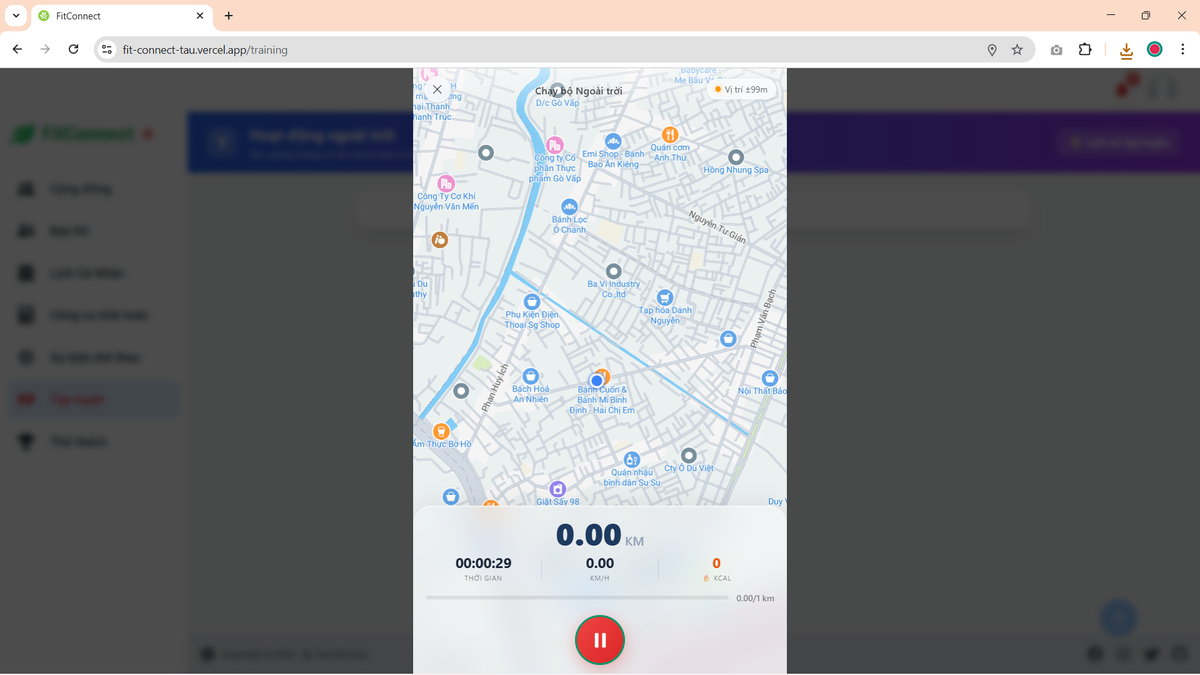
\includegraphics[width=0.60\textwidth]{Images/IMG/nhom5/manhinhtrackinggpstapluyen.png}
    \caption{Hệ thống theo dõi GPS thời gian thực trên bản đồ khi chạy bộ ngoài trời}
    \label{fig:impl_train_gps}
\end{figure}


    \item Khi dừng hoạt động, hệ thống tổng kết kết quả: quãng đường (km), thời gian, và kcal đã đốt. Người dùng nhấn ``Xác nhận'' để lưu vào lịch sử hoặc ``Quay lại'' để tiếp tục hoạt động.

\end{itemize}

\subsubsection{Lưu giáo án và đặt lịch tập}

\begin{itemize}
    \item Tại bước Chuẩn bị tập luyện, khi nhấn ``Lưu bài tập'', hệ thống hiển thị modal ``Lưu bài tập'' yêu cầu nhập tên bài tập (ví dụ: ``Tập lưng'') và hiển thị thông tin tóm tắt (số bài, số sets sẽ được lưu). Người dùng nhấn ``Tiếp tục'' để lưu.

\begin{figure}[H]
    \centering
    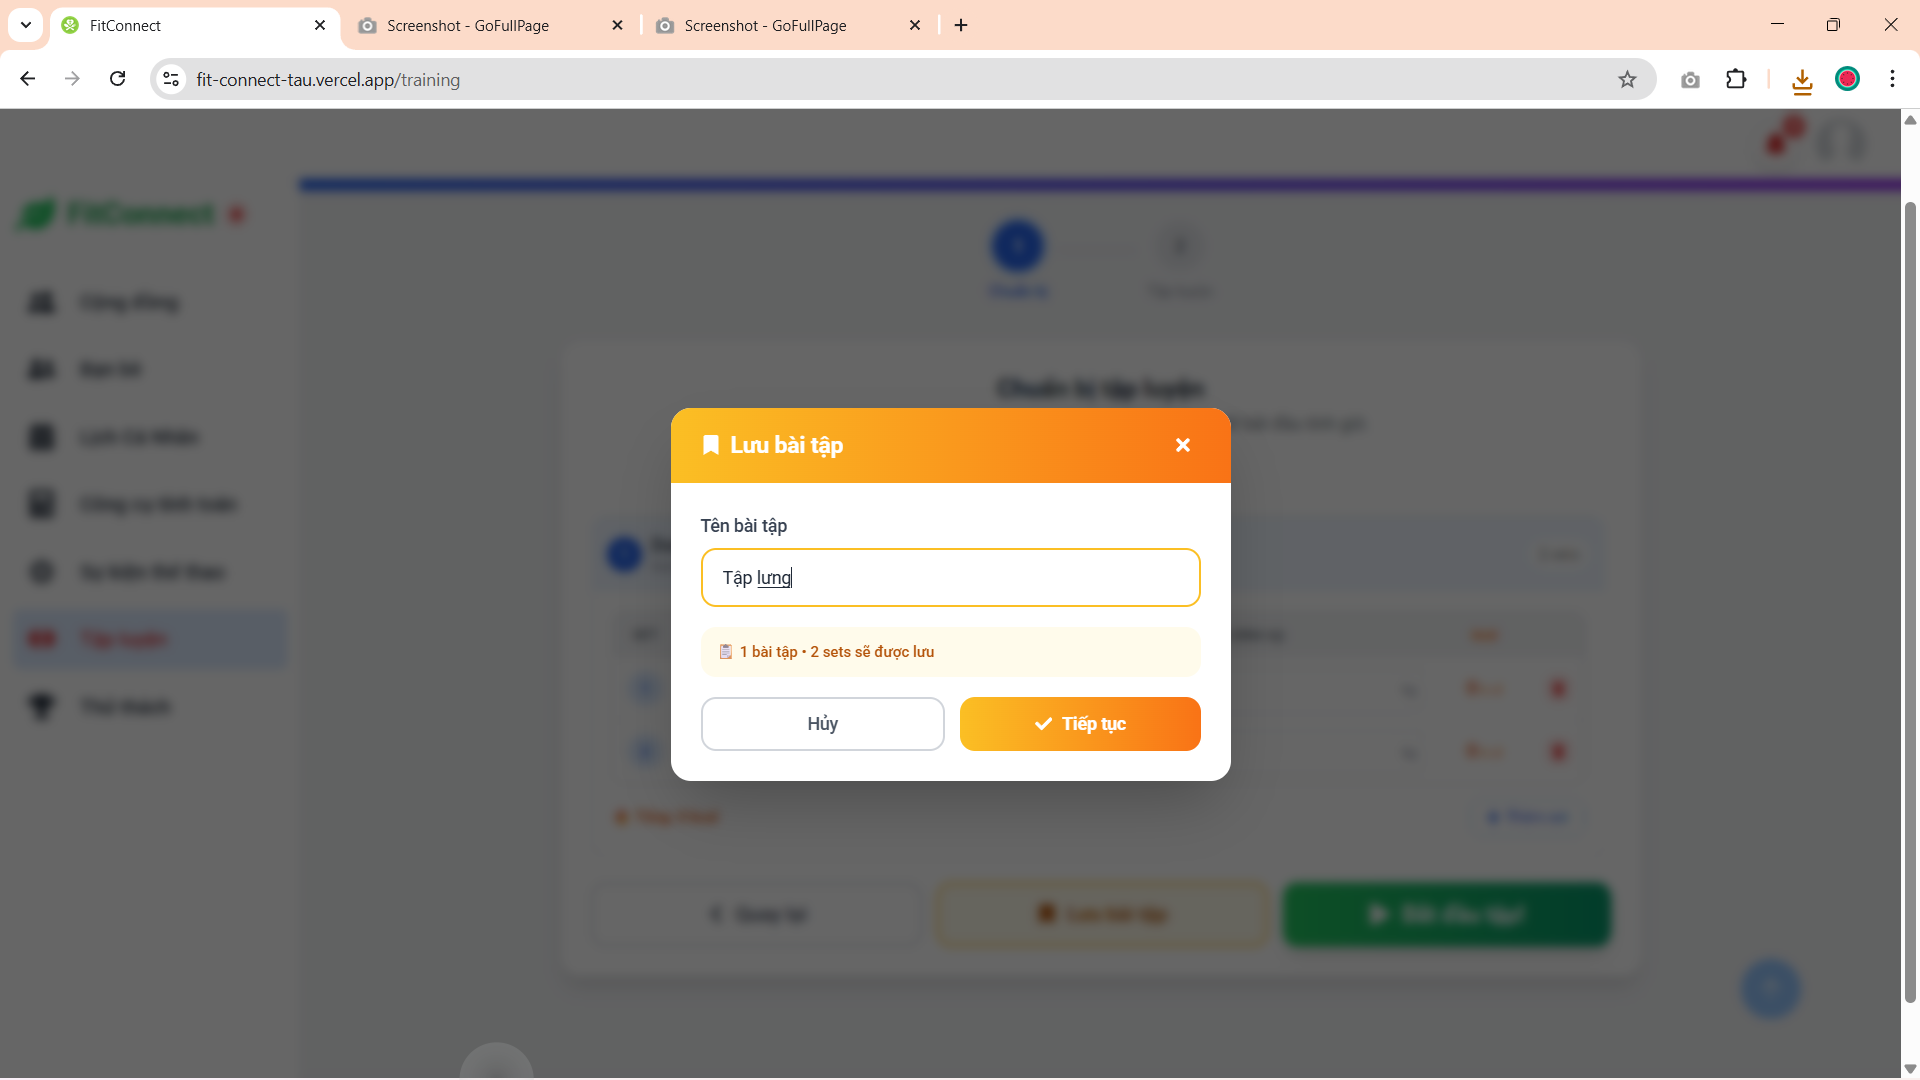
\includegraphics[width=0.60\textwidth]{Images/IMG/nhom5/modalluulichtap.png}
    \caption{Người dùng nhập tên và lưu giáo án tập luyện}
    \label{fig:impl_train_save}
\end{figure}


    \item Sau khi lưu, hệ thống hiển thị modal ``Đặt lịch tập?'' hỏi người dùng có muốn đặt lịch tập định kỳ không. Nếu chọn ``Đặt lịch!'', hệ thống hiển thị modal ``Cài đặt lịch tập'' cho phép chọn: Ngày tập trong tuần (CN, T2, T3,..., T7), Giờ tập, khoảng thời gian (Từ ngày -- Đến ngày), và tùy chọn ``Nhắc nhở khi mở app'' (hiển thị thông báo vào ngày tập theo lịch). Nhấn ``Lưu \& Đặt lịch'' để hoàn tất.

\begin{figure}[H]
    \centering
    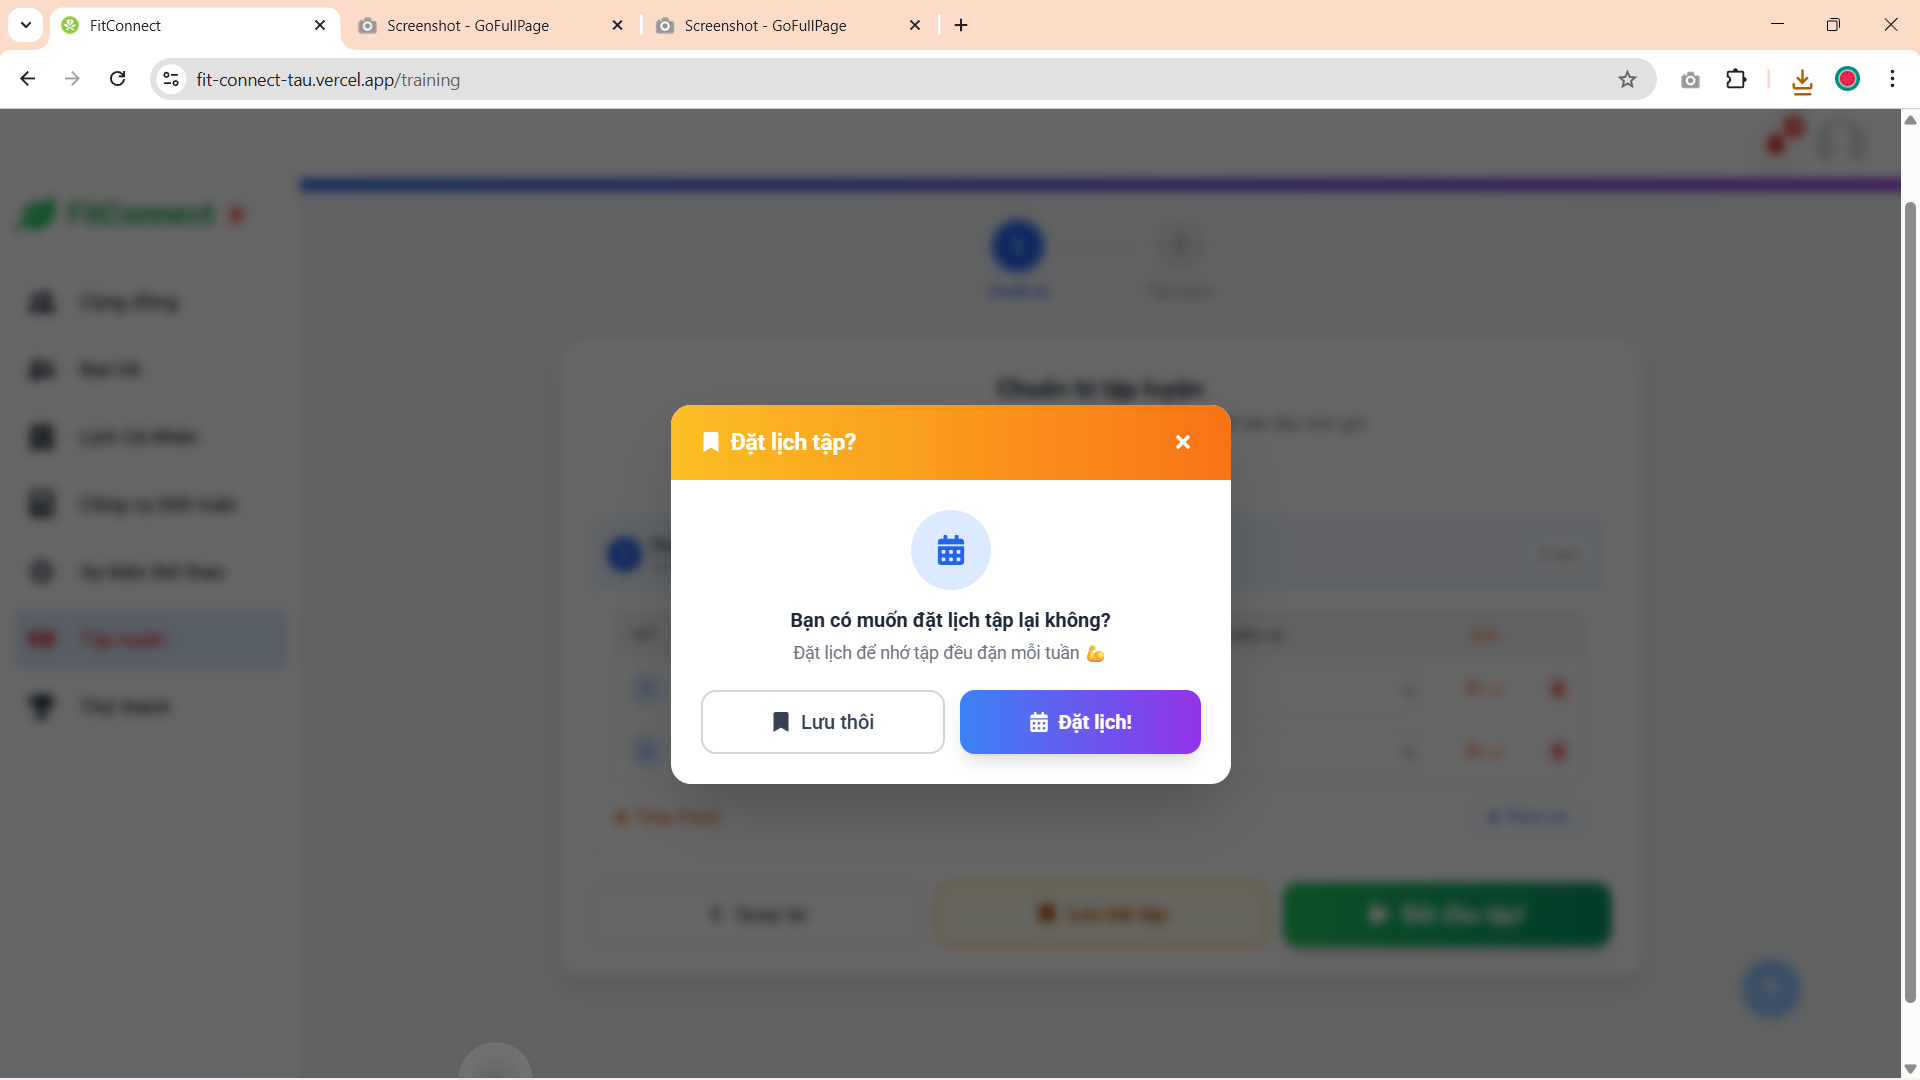
\includegraphics[width=0.60\textwidth]{Images/IMG/nhom5/modaldatlichtap.png}
    \caption{Người dùng cài đặt lịch tập định kỳ với ngày, giờ và nhắc nhở}
    \label{fig:impl_train_schedule}
\end{figure}


    \item Khi chọn chế độ ``Bài tập đã lưu'' từ trang chủ Tập luyện, hệ thống hiển thị modal ``Bài tập đã lưu'' với danh sách giáo án đã lưu, mỗi giáo án hiển thị: tên, số bài tập, số sets, ngày lưu, lịch tập đã đặt (ví dụ: T2, T3, T4 lúc 10:00), nút đặt lịch, nút xóa, và nút ``Tập ngay!''.

\begin{figure}[H]
    \centering
    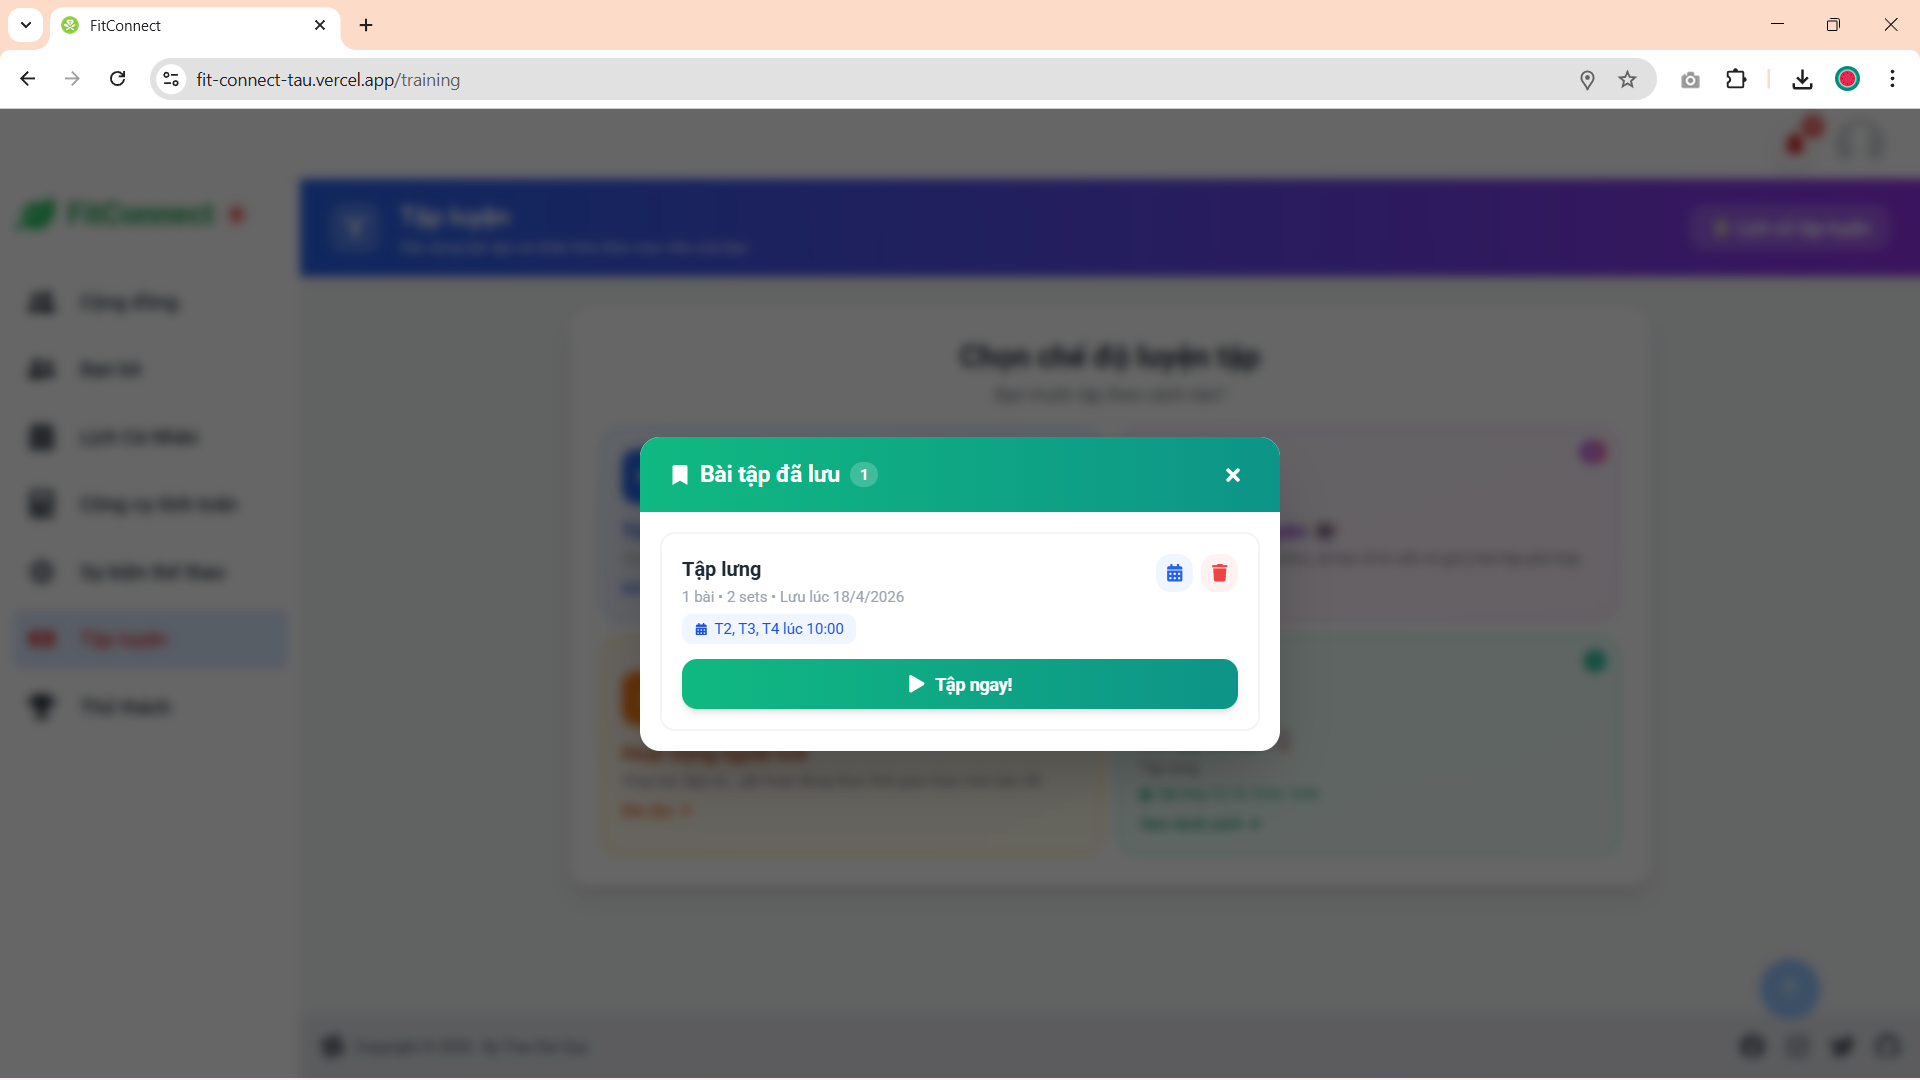
\includegraphics[width=0.60\textwidth]{Images/IMG/nhom5/danhsachbaitapdaluu.png}
    \caption{Hệ thống hiển thị danh sách giáo án tập luyện đã lưu}
    \label{fig:impl_train_saved_list}
\end{figure}

\end{itemize}

\subsubsection{Lịch sử tập luyện}

\begin{itemize}
    \item Người dùng nhấn ``Lịch sử tập luyện'' từ góc phải trang Tập luyện. Hệ thống chuyển sang trang Lịch sử tập luyện hiển thị 2 tab: ``Thời gian trong gym'' và ``Hoạt động ngoài trời''. Tại tab Thời gian trong gym, hệ thống hiển thị bộ lọc thời gian (7 ngày, 30 ngày,...), tổng số hoạt động và tổng thời gian tập. Mỗi buổi tập hiển thị: số bài tập, trạng thái (Hoàn thành), ngày giờ, tổng SETS, tổng KCAL, thời gian (PHÚT), chi tiết từng bài tập kèm số set, và danh sách nhóm cơ cùng thiết bị đã tập.

\begin{figure}[H]
    \centering
    
\includegraphics[width=0.60\textwidth]{Images/IMG/nhom5/lichsutapluyen.png}
    \caption{Hệ thống hiển thị lịch sử tập luyện trong gym với chi tiết từng buổi tập}
    \label{fig:impl_train_history_gym}
\end{figure}


    \item Tại tab ``Hoạt động ngoài trời'', hệ thống hiển thị danh sách các hoạt động ngoài trời đã thực hiện. Mỗi hoạt động hiển thị: tên bài tập, loại hoạt động, ngày giờ, quãng đường (km), tốc độ (km/h), kcal đã đốt, và thời gian.

\begin{figure}[H]
    \centering
    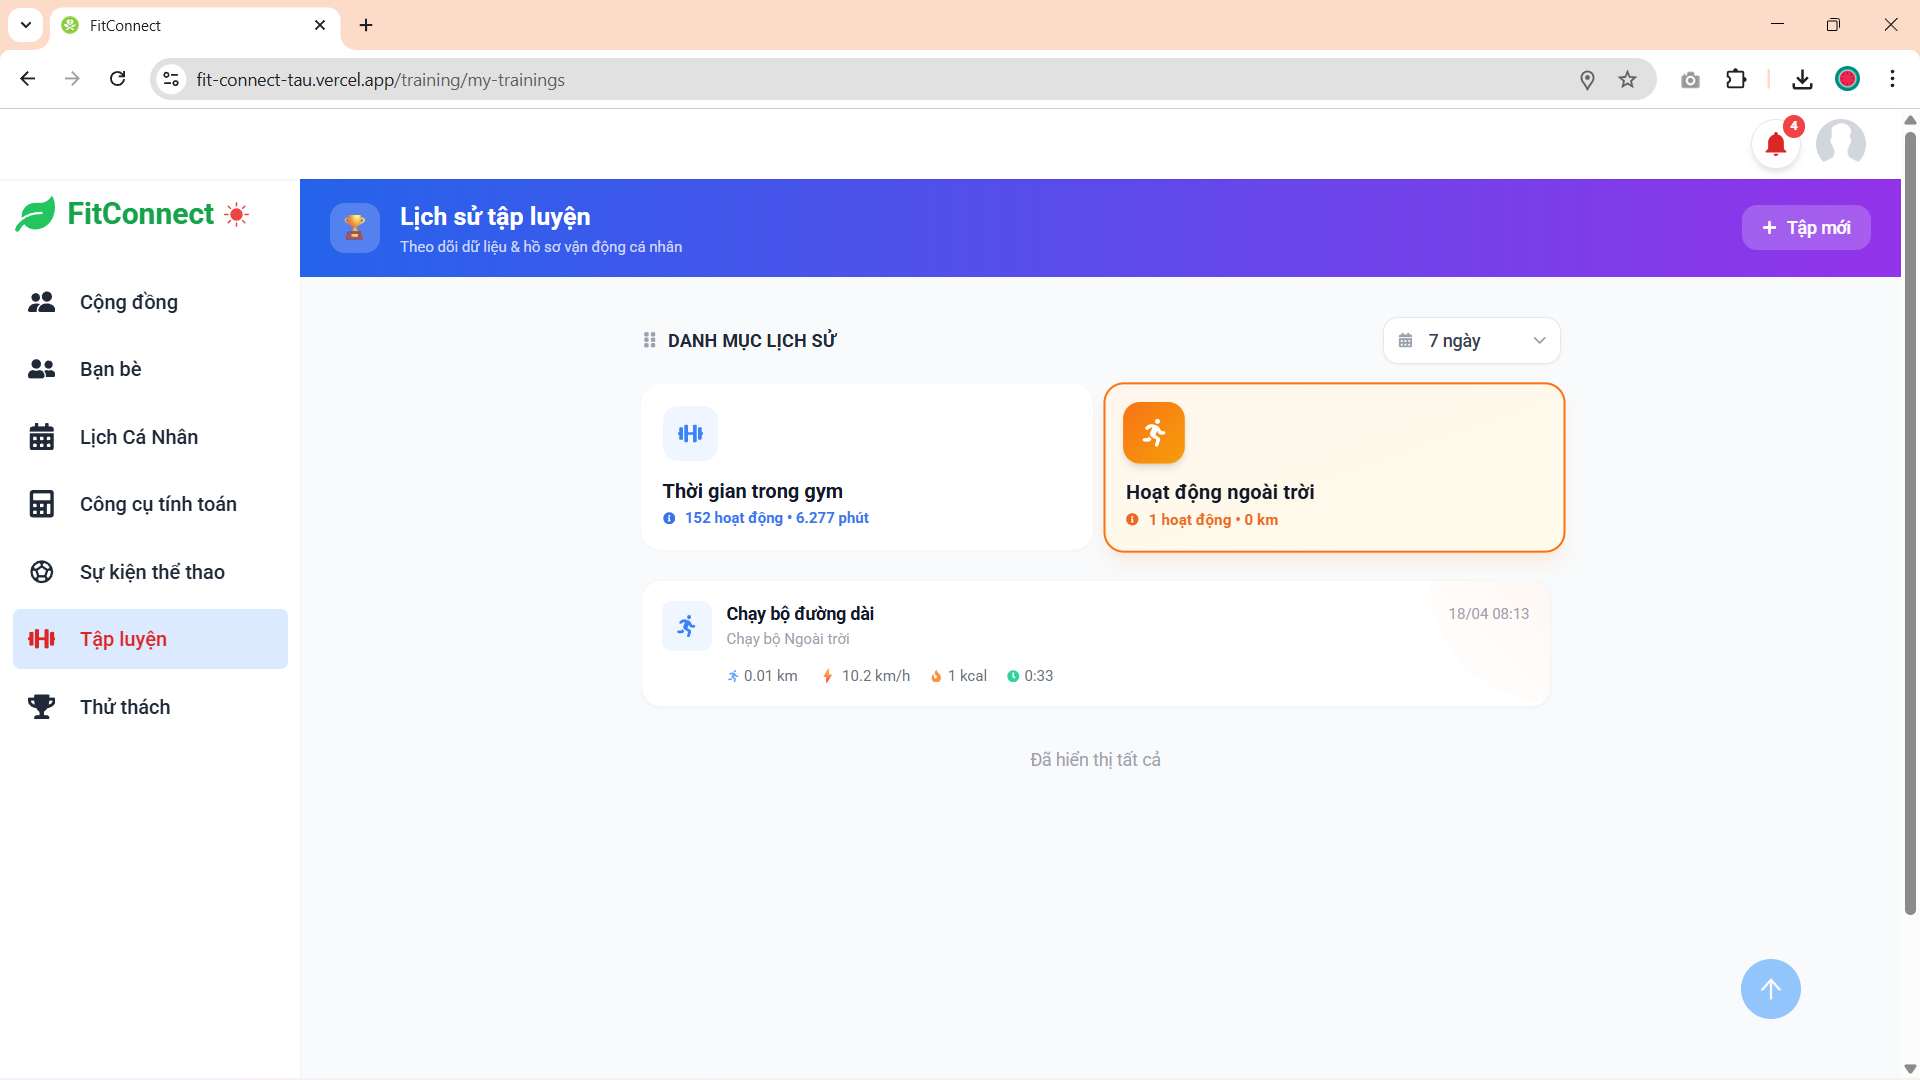
\includegraphics[width=0.60\textwidth]{Images/IMG/nhom5/lichsusaukhitapluyenchayboxong.png}
    \caption{Hệ thống hiển thị lịch sử hoạt động ngoài trời với thông số chi tiết}
    \label{fig:impl_train_history_outdoor}
\end{figure}

\end{itemize}

\subsection{Nhóm tính năng Lịch cá nhân và Thông báo}
\label{subsec:impl_calendar_notification}

Nhóm tính năng Lịch cá nhân và Thông báo giúp người dùng quản lý lịch hoạt động theo thời gian, theo dõi các đầu việc quan trọng trong ngày, đồng thời tiếp nhận các tương tác và cập nhật hệ thống theo thời gian thực. Lịch cá nhân đóng vai trò trung tâm tổng hợp các nguồn dữ liệu từ lịch tập luyện đã lưu, sự kiện thể thao đã tham gia và thử thách đang theo đuổi; trong khi trung tâm thông báo hỗ trợ phân loại, đánh dấu đã đọc, điều hướng nhanh đến nội dung liên quan và quản lý thông báo thuận tiện ngay trên thanh tiêu đề.

\subsubsection{Luồng thao tác trên Lịch cá nhân}
\begin{itemize}
    \item Người dùng truy cập mục ``Lịch Cá Nhân'' từ thanh điều hướng bên trái. Hệ thống hiển thị giao diện lịch tổng quan, kết hợp các hoạt động theo mốc thời gian gồm: sự kiện thể thao, lịch tập luyện và thử thách. Tại phần điều khiển, người dùng có thể chuyển nhanh về ``Hôm nay'', điều hướng tháng/tuần kế tiếp, đồng thời bật/tắt từng nhóm dữ liệu để tập trung vào nội dung cần theo dõi.

\begin{figure}[H]
    \centering
    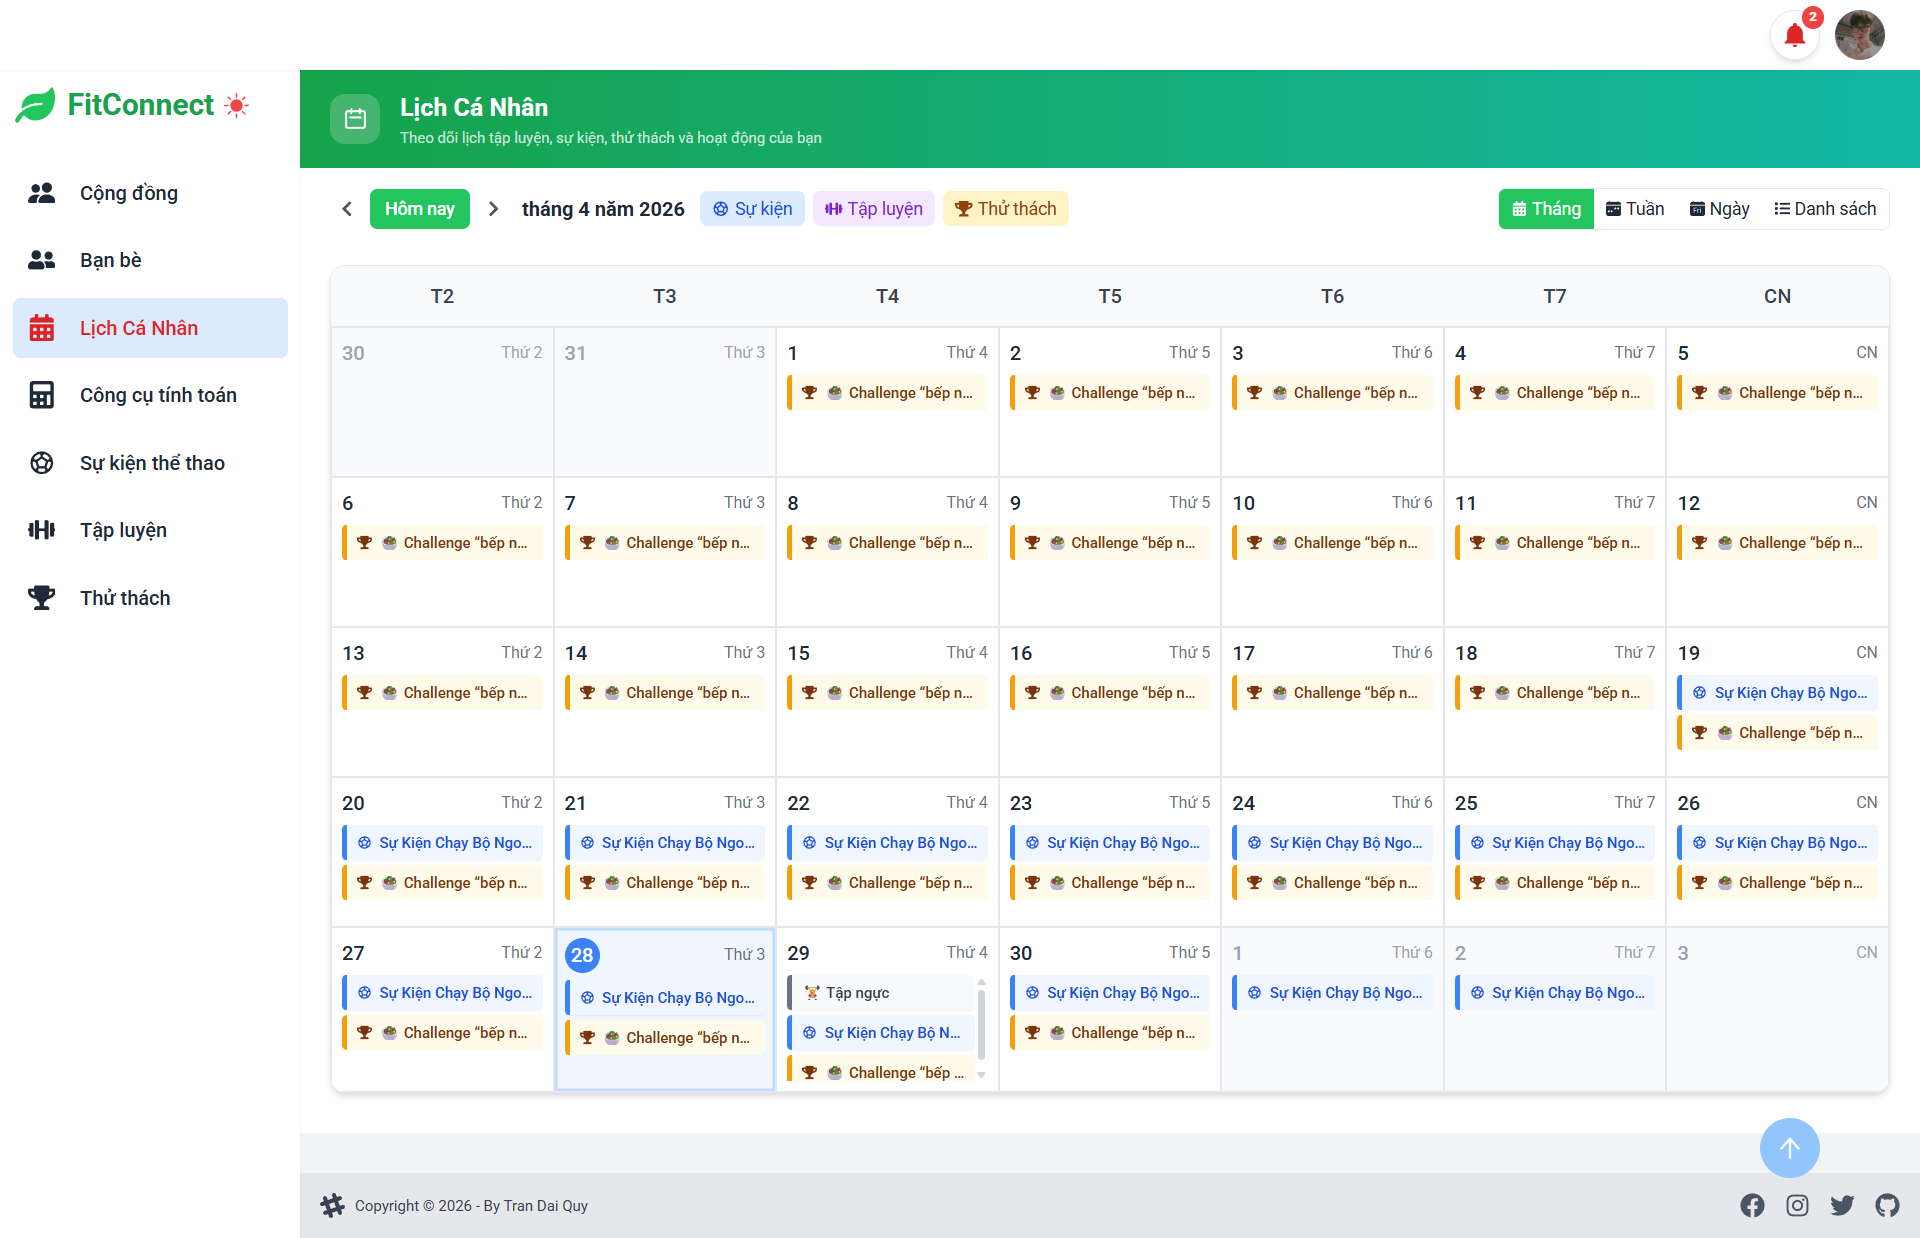
\includegraphics[width=0.60\textwidth]{Images/IMG/nhom8/tranglichcanhan.png}
    \caption{Hệ thống hiển thị trang Lịch cá nhân với bộ lọc theo loại hoạt động}
    \label{fig:impl_cal_main}
\end{figure}


    \item Ở chế độ ``Tháng'', người dùng quan sát toàn bộ kế hoạch trong tháng hiện tại dưới dạng lưới ngày. Mỗi ô ngày hiển thị rút gọn các hoạt động chính và cho phép nhấn để xem nhanh hoạt động phát sinh trong ngày đó, phù hợp cho việc theo dõi tổng quan và phát hiện các ngày có mật độ hoạt động cao.

\begin{figure}[H]
    \centering
    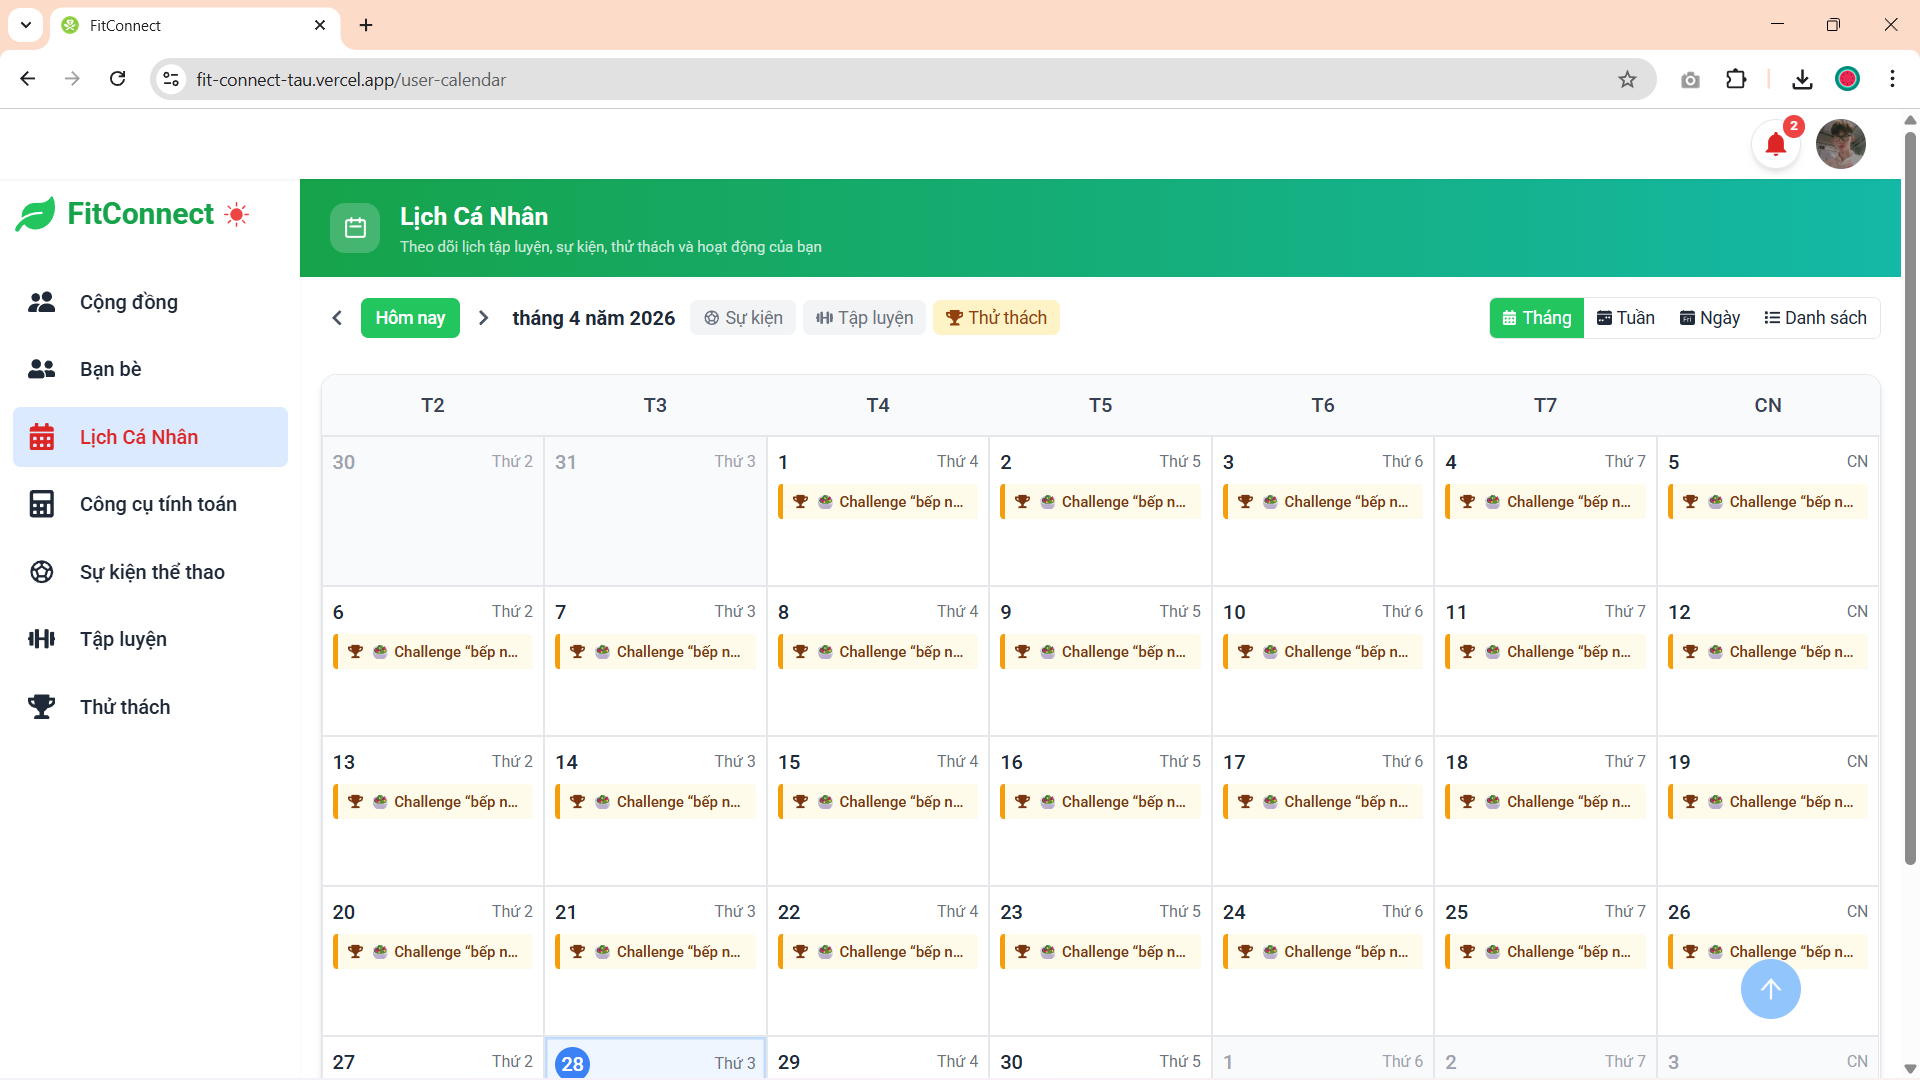
\includegraphics[width=0.60\textwidth]{Images/IMG/nhom8/chedothangtrangtongquan.png}
    \caption{Người dùng theo dõi lịch hoạt động ở chế độ Tháng}
    \label{fig:impl_cal_month}
\end{figure}


    \item Người dùng có thể chuyển sang các chế độ ``Tuần'', ``Ngày'' và ``Danh sách'' để xem lịch theo mức độ chi tiết khác nhau. Chế độ Tuần và Ngày hiển thị timeline theo giờ giúp quản lý khung thời gian tập luyện/sự kiện cụ thể; chế độ Danh sách gom sự kiện theo ngày, phù hợp khi cần quét nhanh toàn bộ hoạt động trong tháng.

\begin{figure}[H]
    \centering
    \begin{subfigure}[b]{0.30\textwidth}
        \centering
        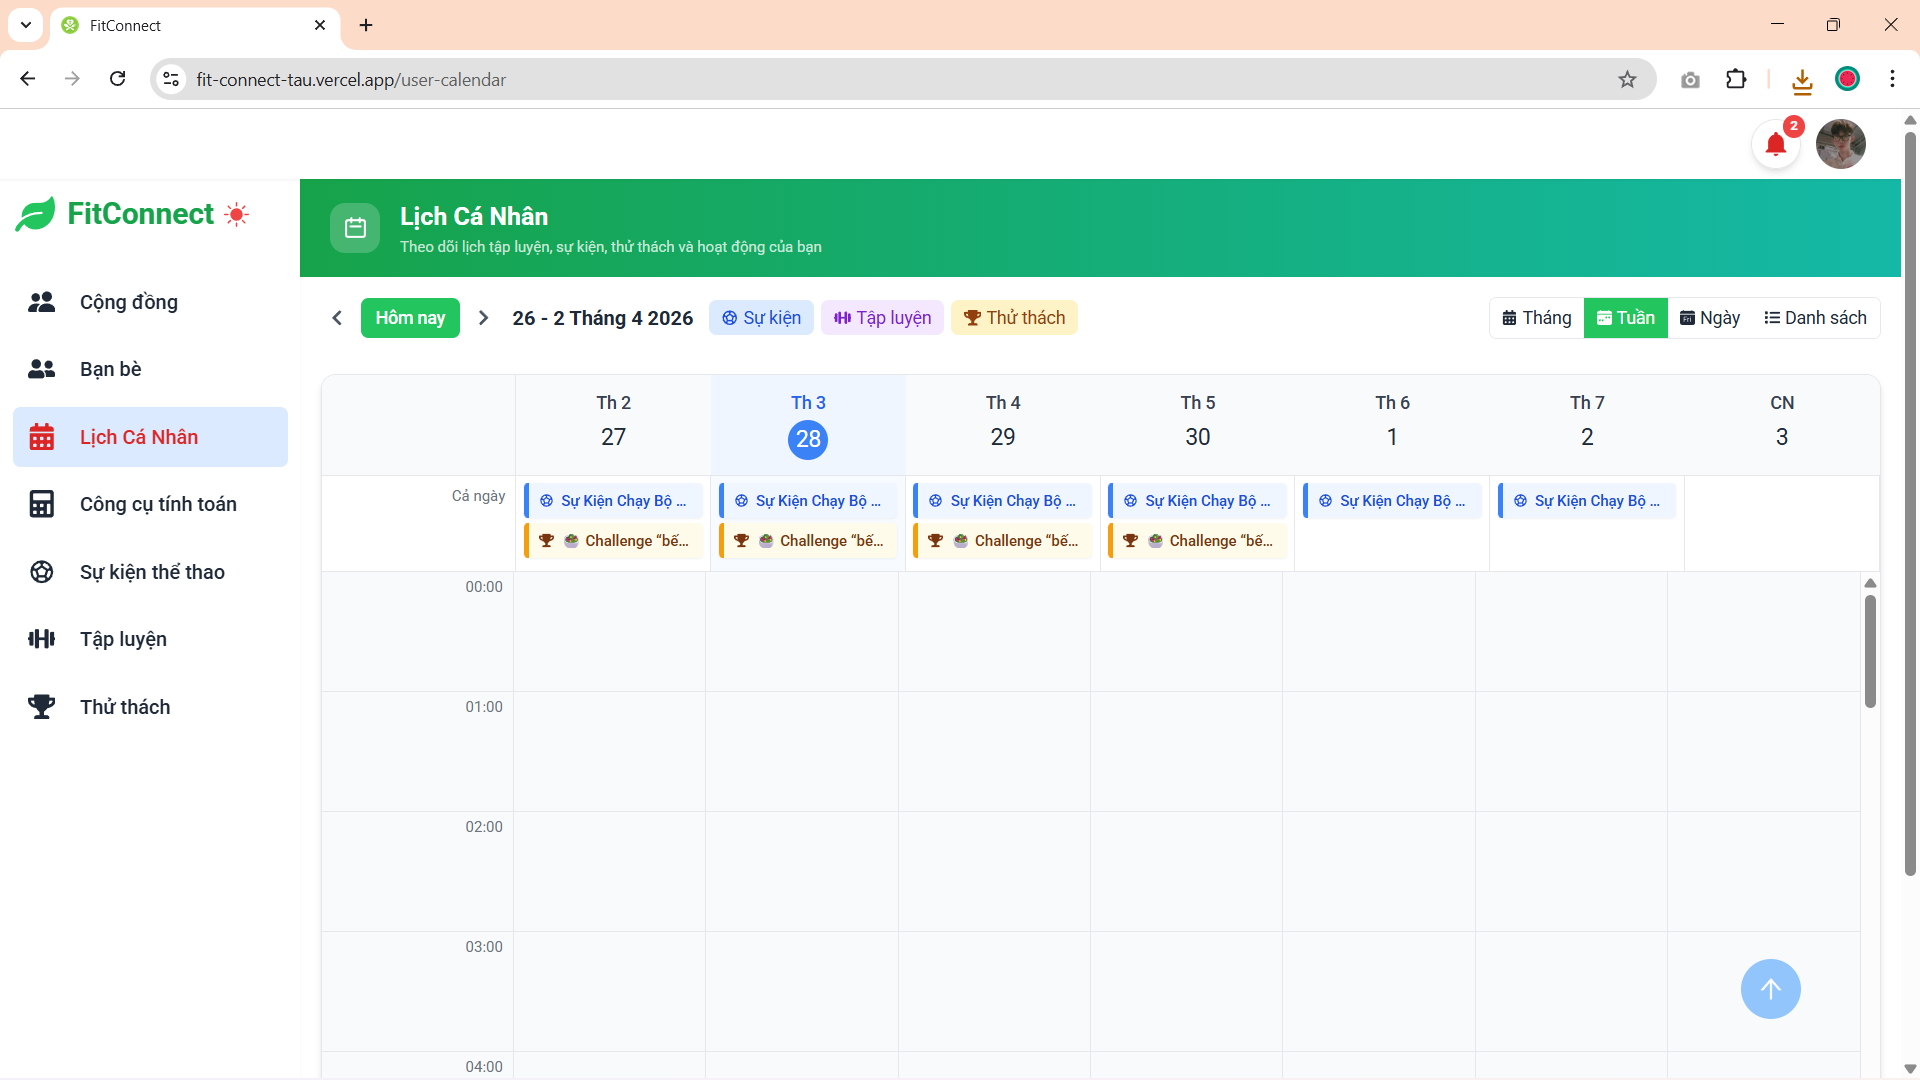
\includegraphics[width=\textwidth]{Images/IMG/nhom8/chedotuan.png}
        \caption{Hệ thống hiển thị lịch cá nhân ở chế độ Tuần theo khung giờ}
        \label{fig:impl_cal_week}
    \end{subfigure}
    \hfill
    \begin{subfigure}[b]{0.30\textwidth}
        \centering
        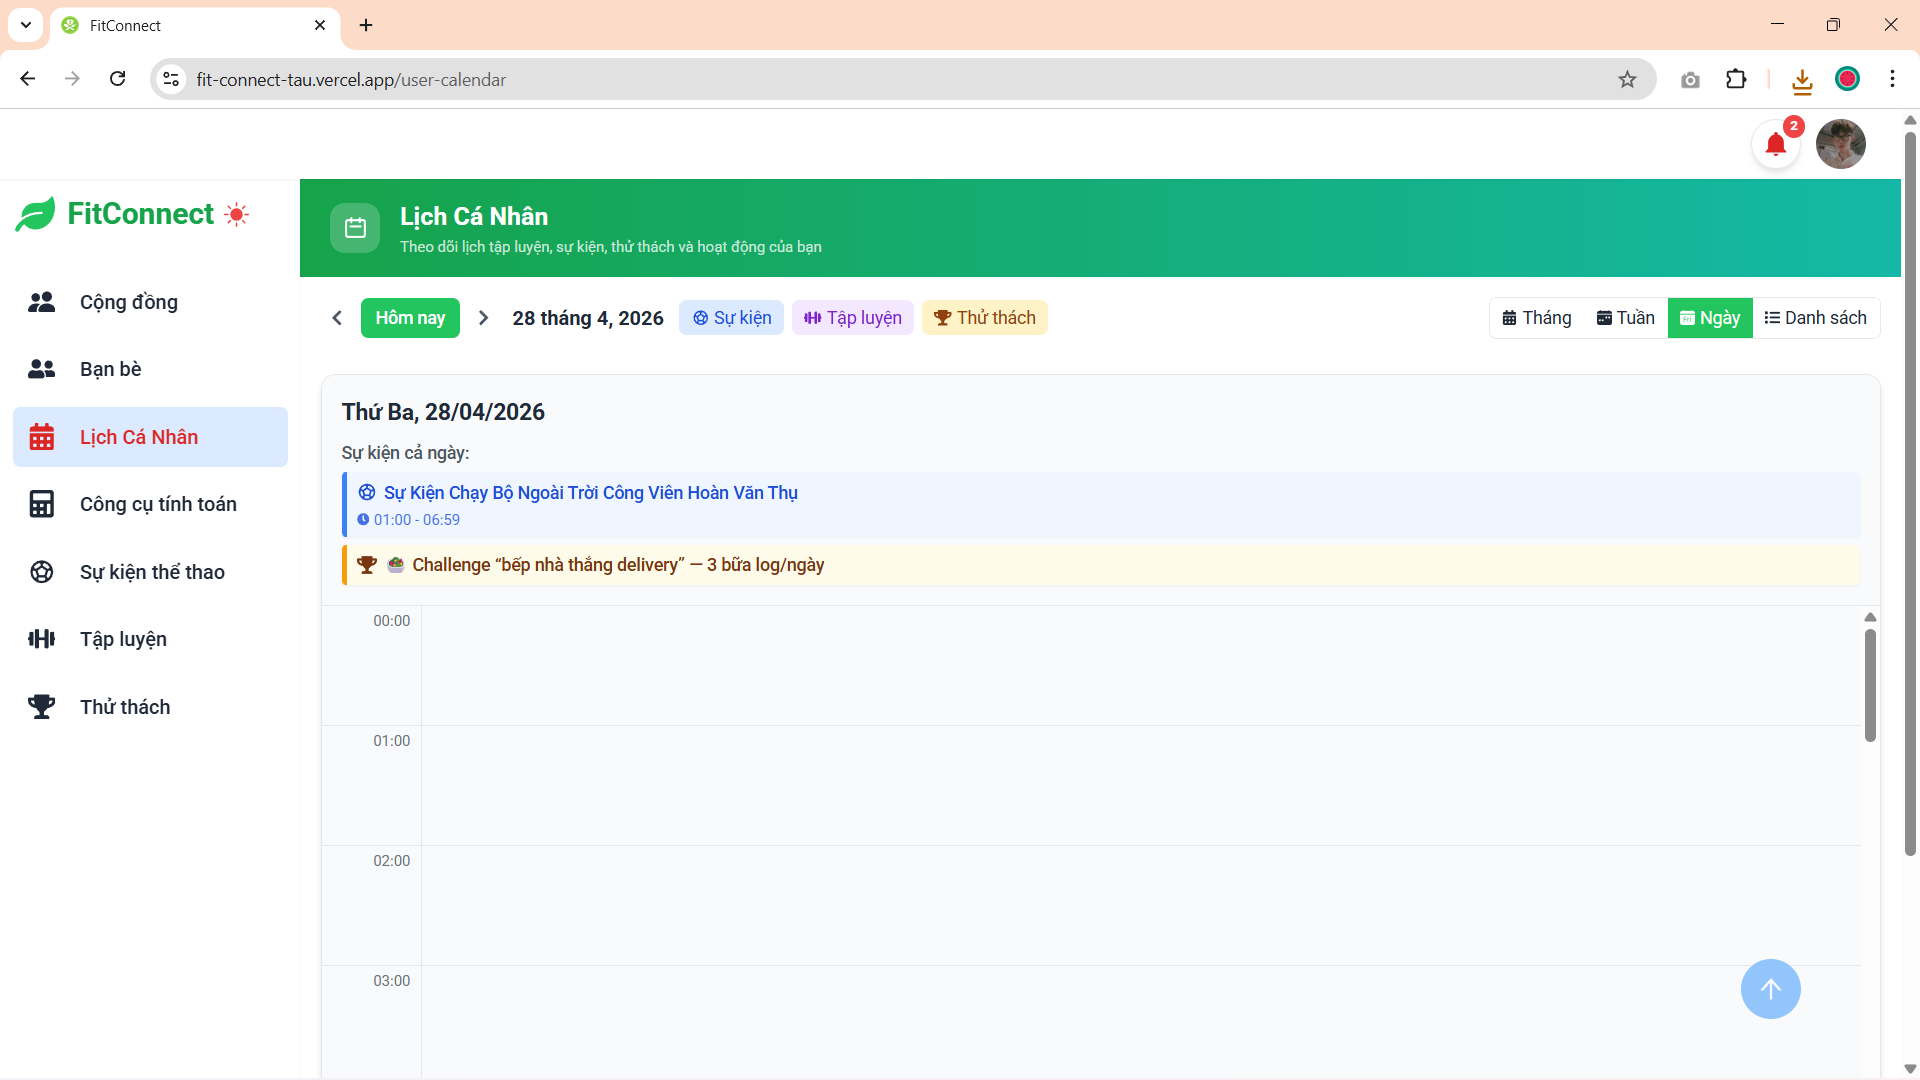
\includegraphics[width=\textwidth]{Images/IMG/nhom8/chedongay.png}
        \caption{Hệ thống hiển thị lịch cá nhân ở chế độ Ngày}
        \label{fig:impl_cal_day}
    \end{subfigure}
    \hfill
    \begin{subfigure}[b]{0.30\textwidth}
        \centering
        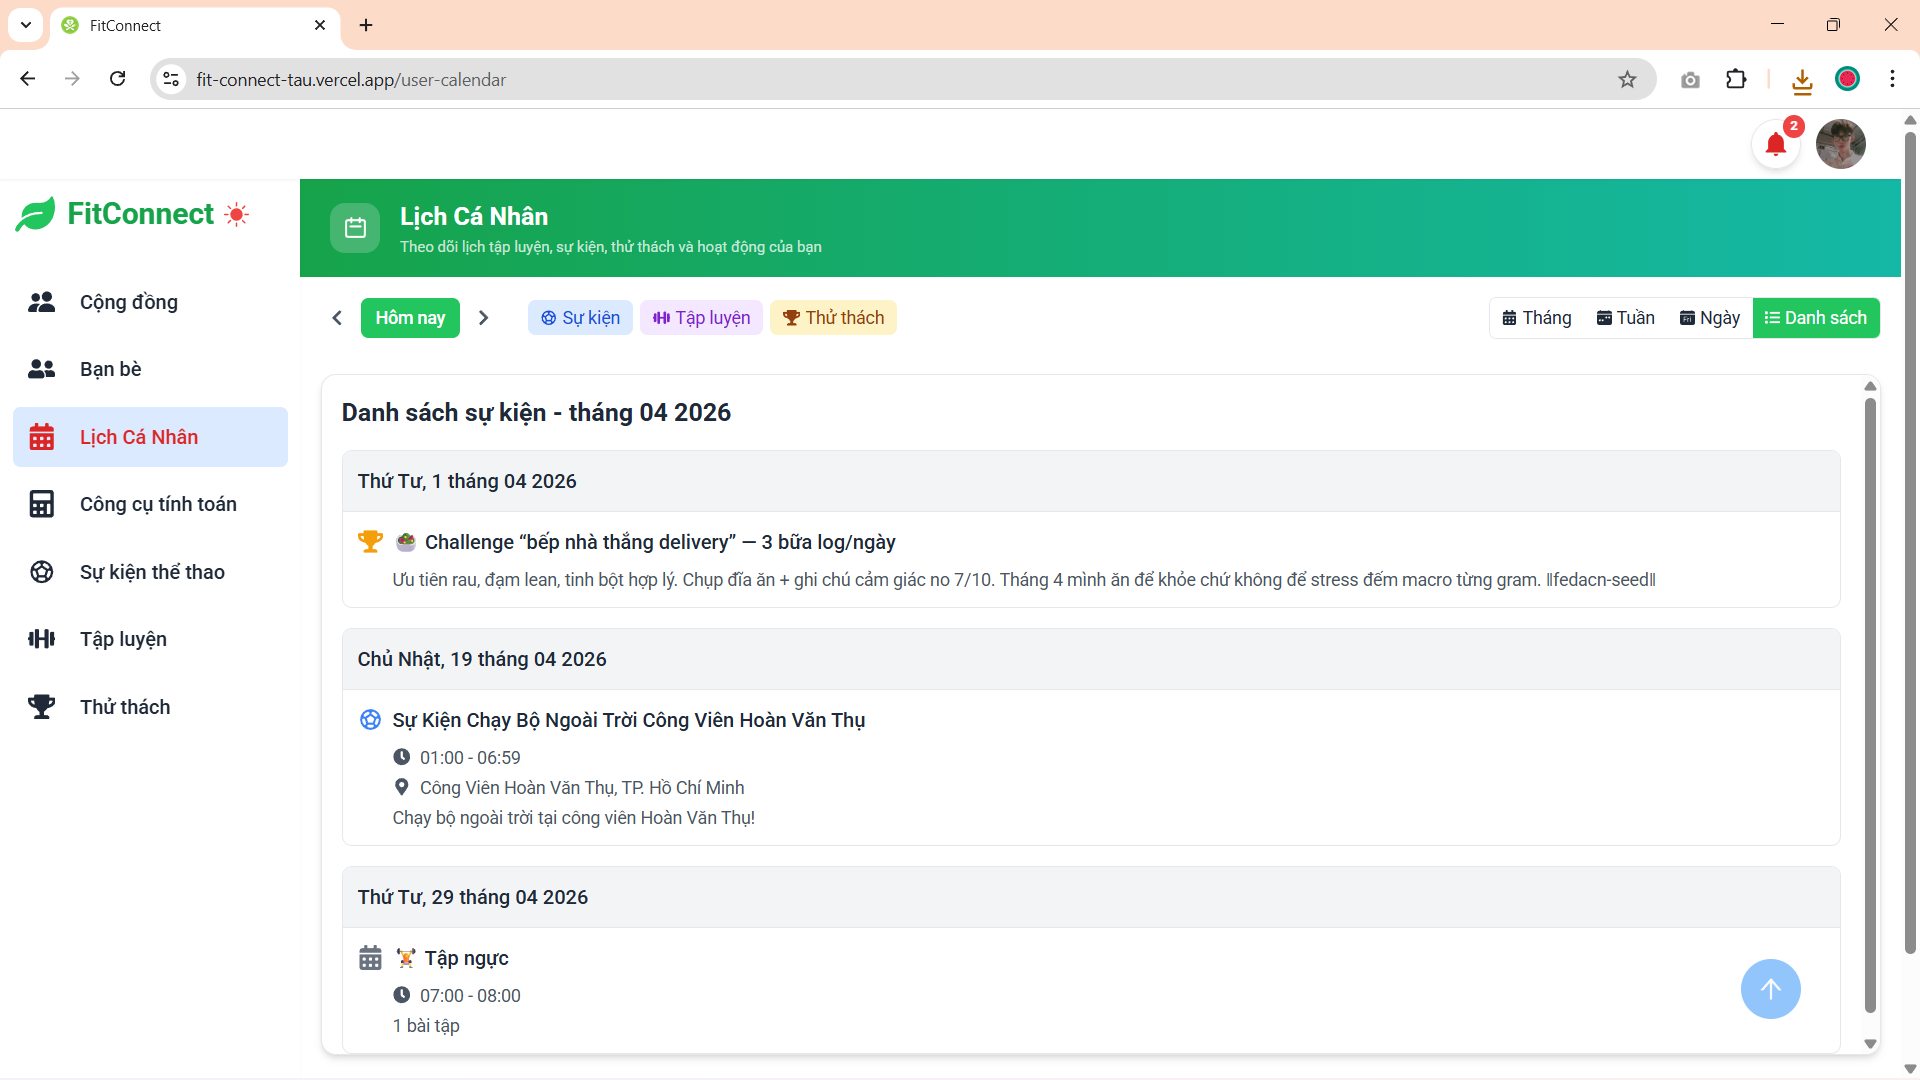
\includegraphics[width=\textwidth]{Images/IMG/nhom8/chedodanhsach.png}
        \caption{Hệ thống hiển thị lịch cá nhân ở chế độ Danh sách}
        \label{fig:impl_cal_agenda}
    \end{subfigure}
\end{figure}


    \item Khi nhấn vào một hoạt động cụ thể trên lịch, hệ thống mở modal chi tiết theo từng ngữ cảnh. Với sự kiện thể thao, người dùng xem được loại sự kiện, thời gian, địa điểm, trạng thái tham gia và thông tin tổ chức.

\begin{figure}[H]
    \centering
    
\includegraphics[width=0.60\textwidth]{Images/IMG/nhom8/chitietsukien.png}
    \caption{Hệ thống hiển thị modal chi tiết sự kiện thể thao từ Lịch cá nhân}
    \label{fig:impl_cal_event_detail}
\end{figure}


    \item Tương tự, khi chọn một thử thách trên lịch, hệ thống hiển thị thông tin tổng quan thử thách gồm trạng thái, mô tả và điều hướng nhanh tới trang thử thách để tiếp tục theo dõi tiến độ.

\begin{figure}[H]
    \centering
    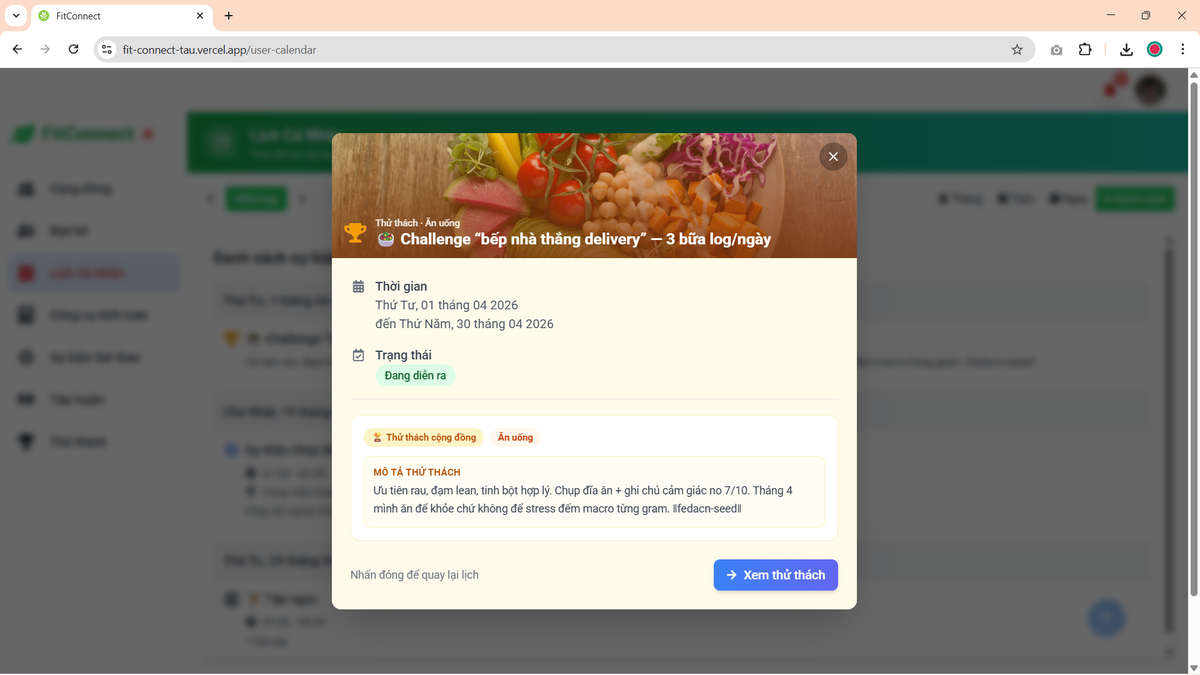
\includegraphics[width=0.60\textwidth]{Images/IMG/nhom8/chitietthuthach.png}
    \caption{Hệ thống hiển thị modal chi tiết thử thách từ Lịch cá nhân}
    \label{fig:impl_cal_challenge_detail}
\end{figure}


    \item Với lịch tập luyện đã lưu, modal chi tiết hiển thị danh sách bài tập, số set và thông tin nhắc nhở; người dùng có thể nhấn ``Tập ngay'' để chuyển trực tiếp sang màn hình tập luyện, giúp rút ngắn thao tác thực thi kế hoạch trong ngày.

\begin{figure}[H]
    \centering
    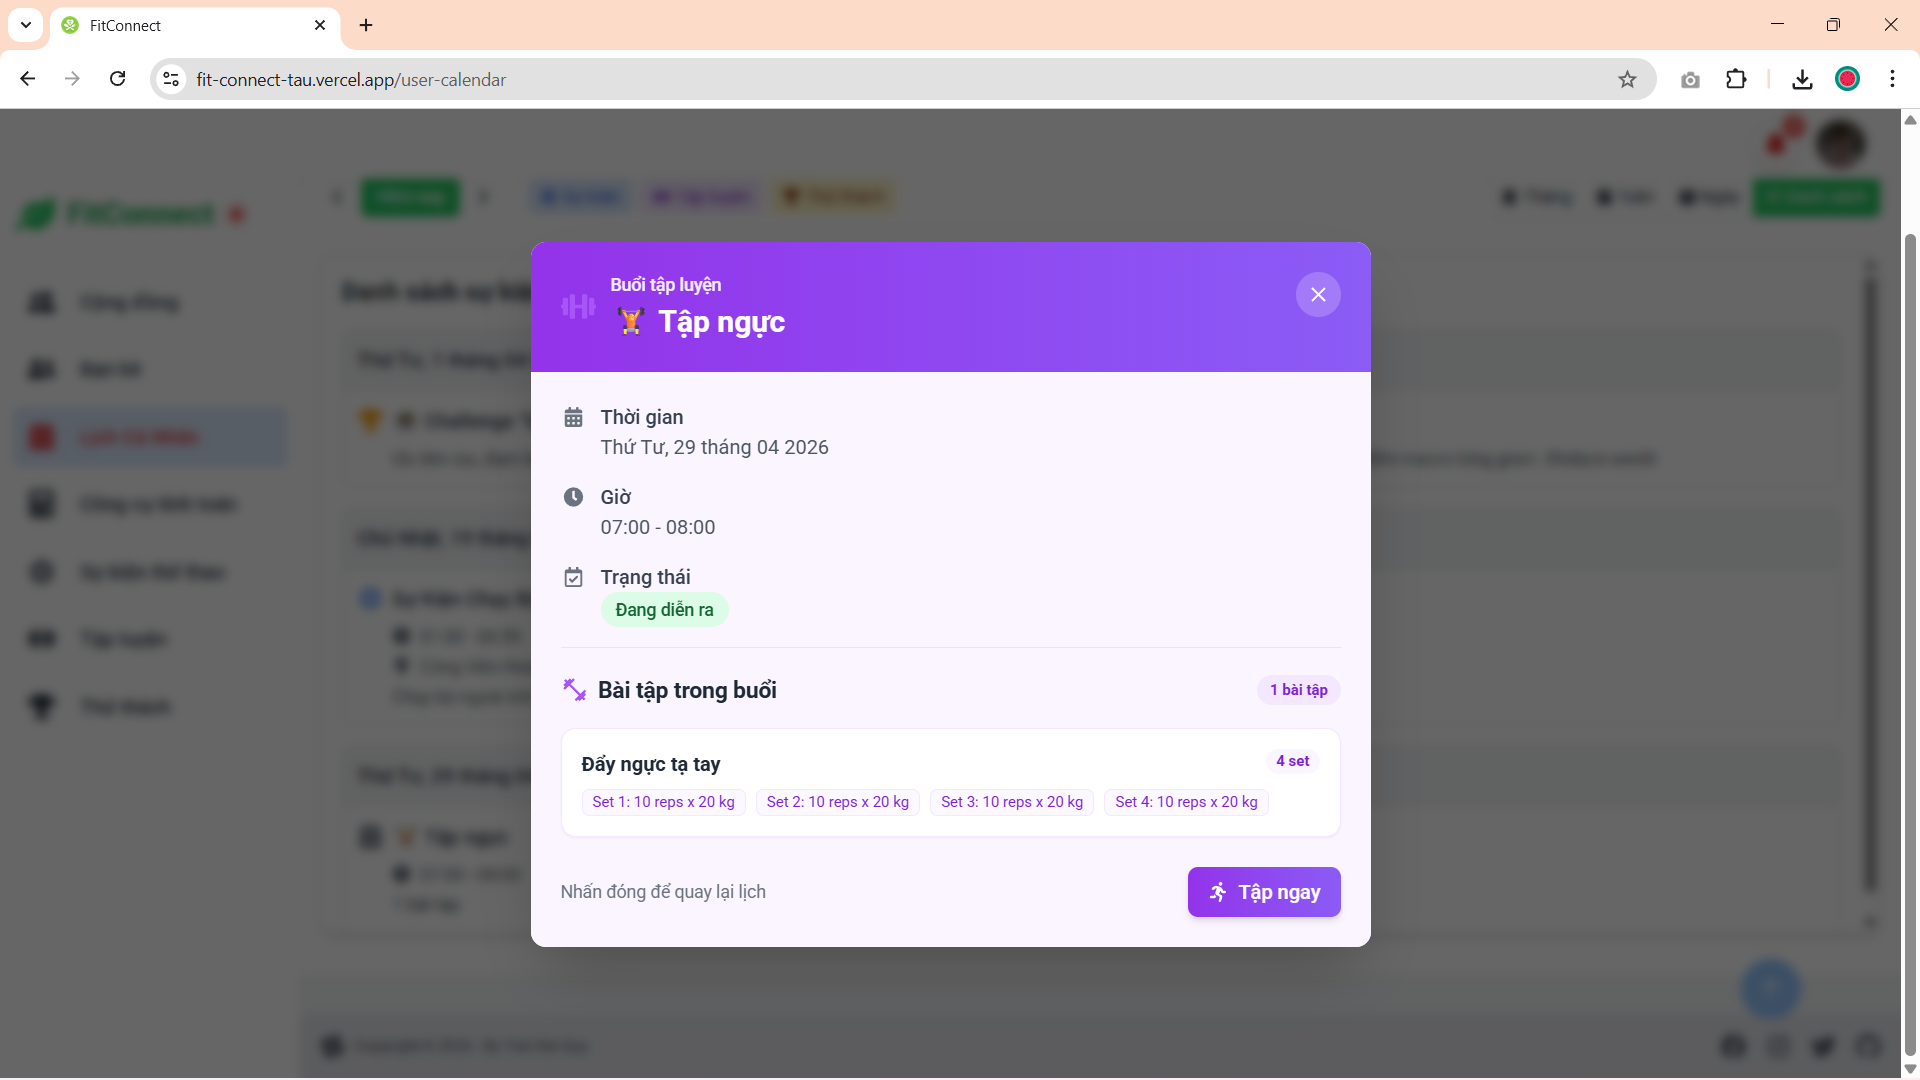
\includegraphics[width=0.60\textwidth]{Images/IMG/nhom8/chitiettapluyen.png}
    \caption{Hệ thống hiển thị modal chi tiết lịch tập luyện và điều hướng tập ngay}
    \label{fig:impl_cal_workout_detail}
\end{figure}


    \item Khi cần theo dõi nhanh công việc trong ngày hiện tại, người dùng nhấn ``Hôm nay'' để đưa lịch về mốc hiện tại và xem các hoạt động phát sinh trong ngày, bao gồm sự kiện, thử thách và buổi tập đã lên lịch.

\begin{figure}[H]
    \centering
    \begin{subfigure}[b]{0.30\textwidth}
        \centering
        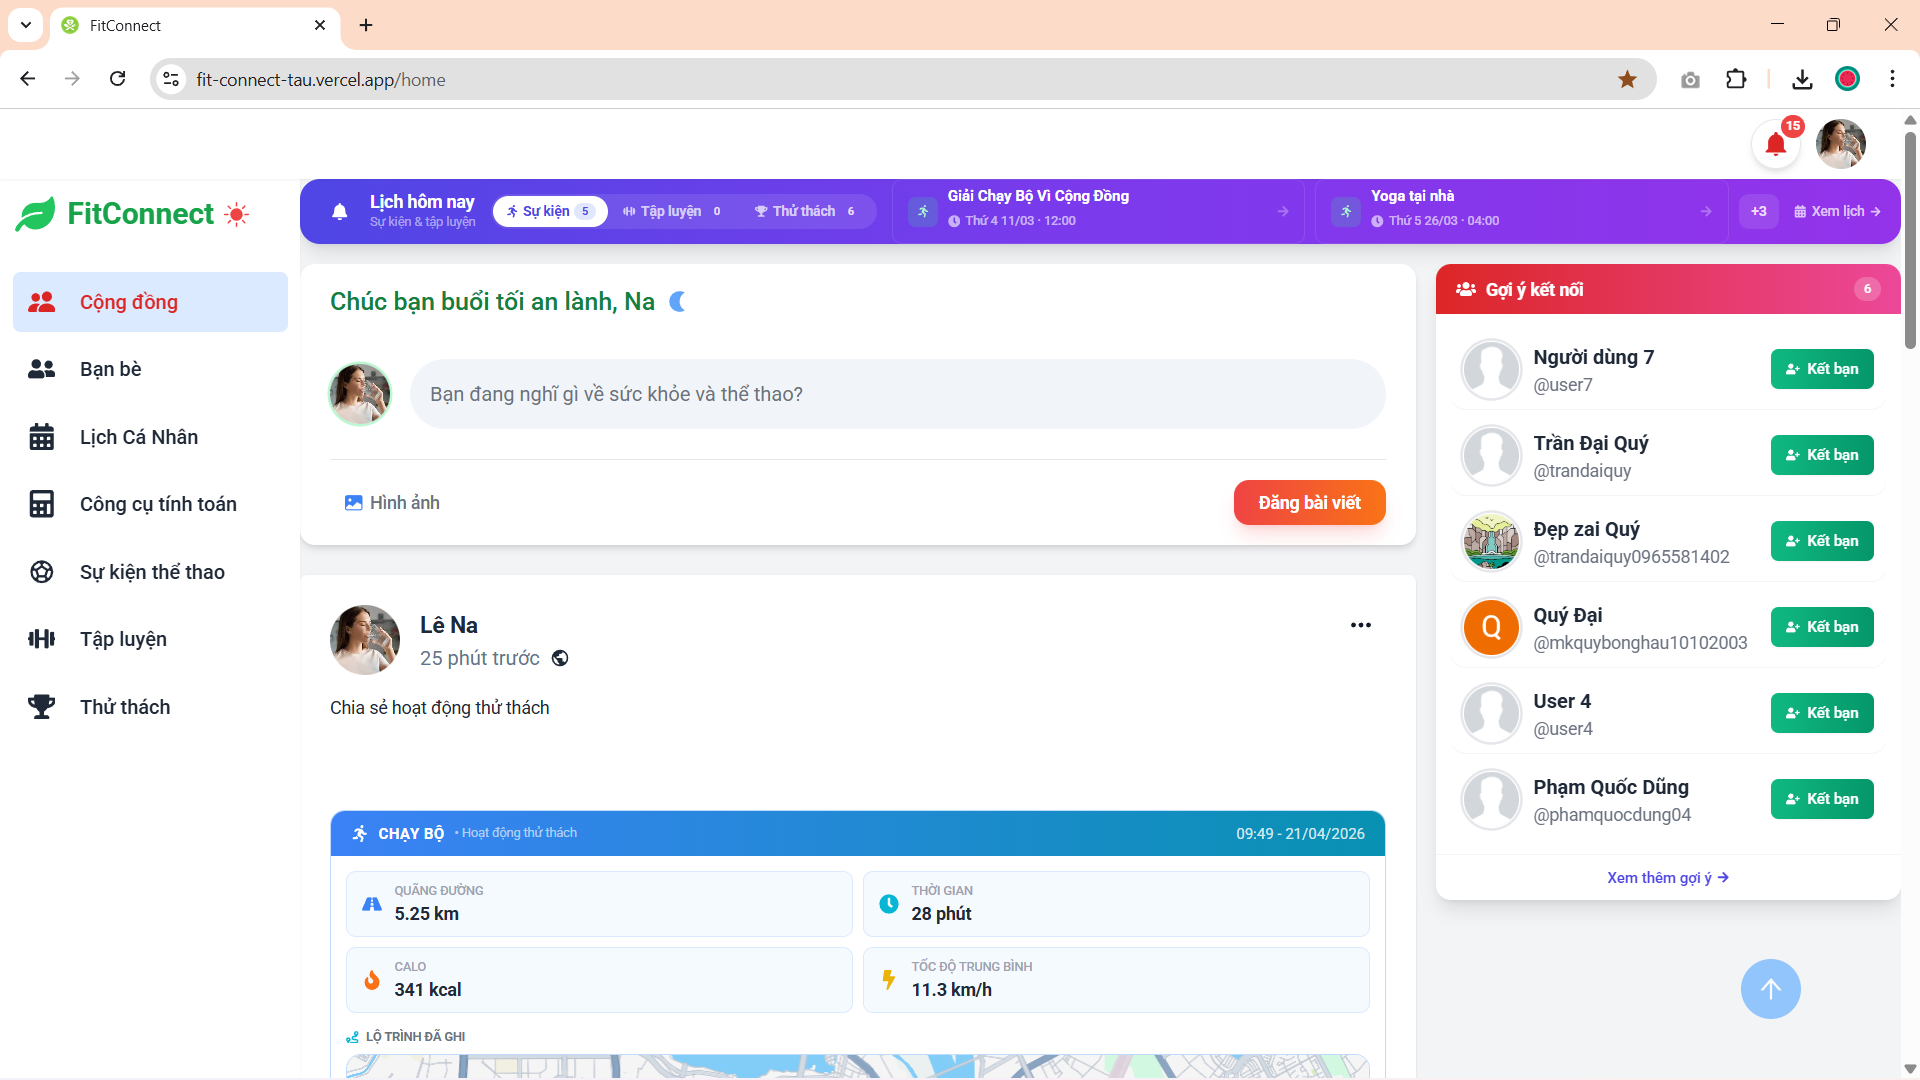
\includegraphics[width=\textwidth]{Images/IMG/nhom8/lichhomnaysukien.png}
        \caption{Người dùng theo dõi hoạt động sự kiện trong ngày hiện tại}
        \label{fig:impl_cal_today_event}
    \end{subfigure}
    \hfill
    \begin{subfigure}[b]{0.30\textwidth}
        \centering
        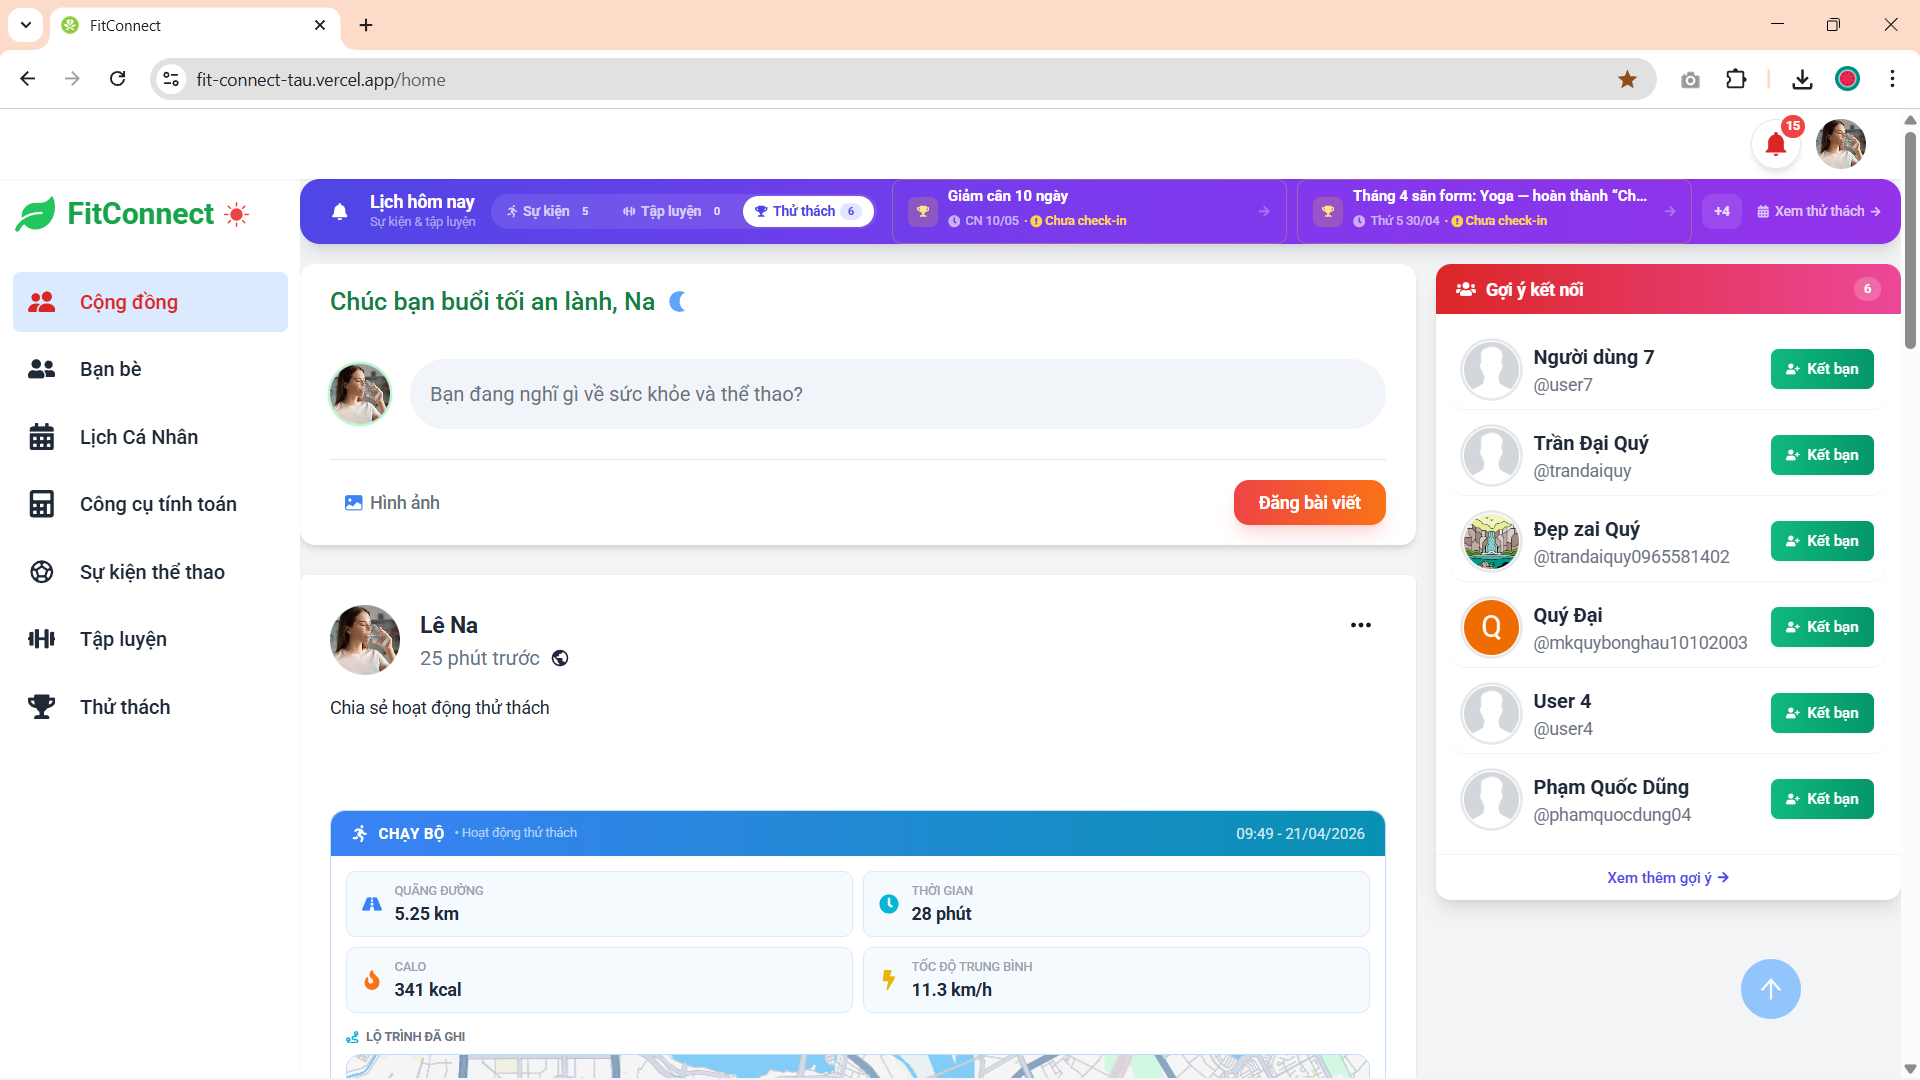
\includegraphics[width=\textwidth]{Images/IMG/nhom8/lichhomnaythuthach.png}
        \caption{Người dùng theo dõi hoạt động thử thách trong ngày hiện tại}
        \label{fig:impl_cal_today_challenge}
    \end{subfigure}
    \hfill
    \begin{subfigure}[b]{0.30\textwidth}
        \centering
        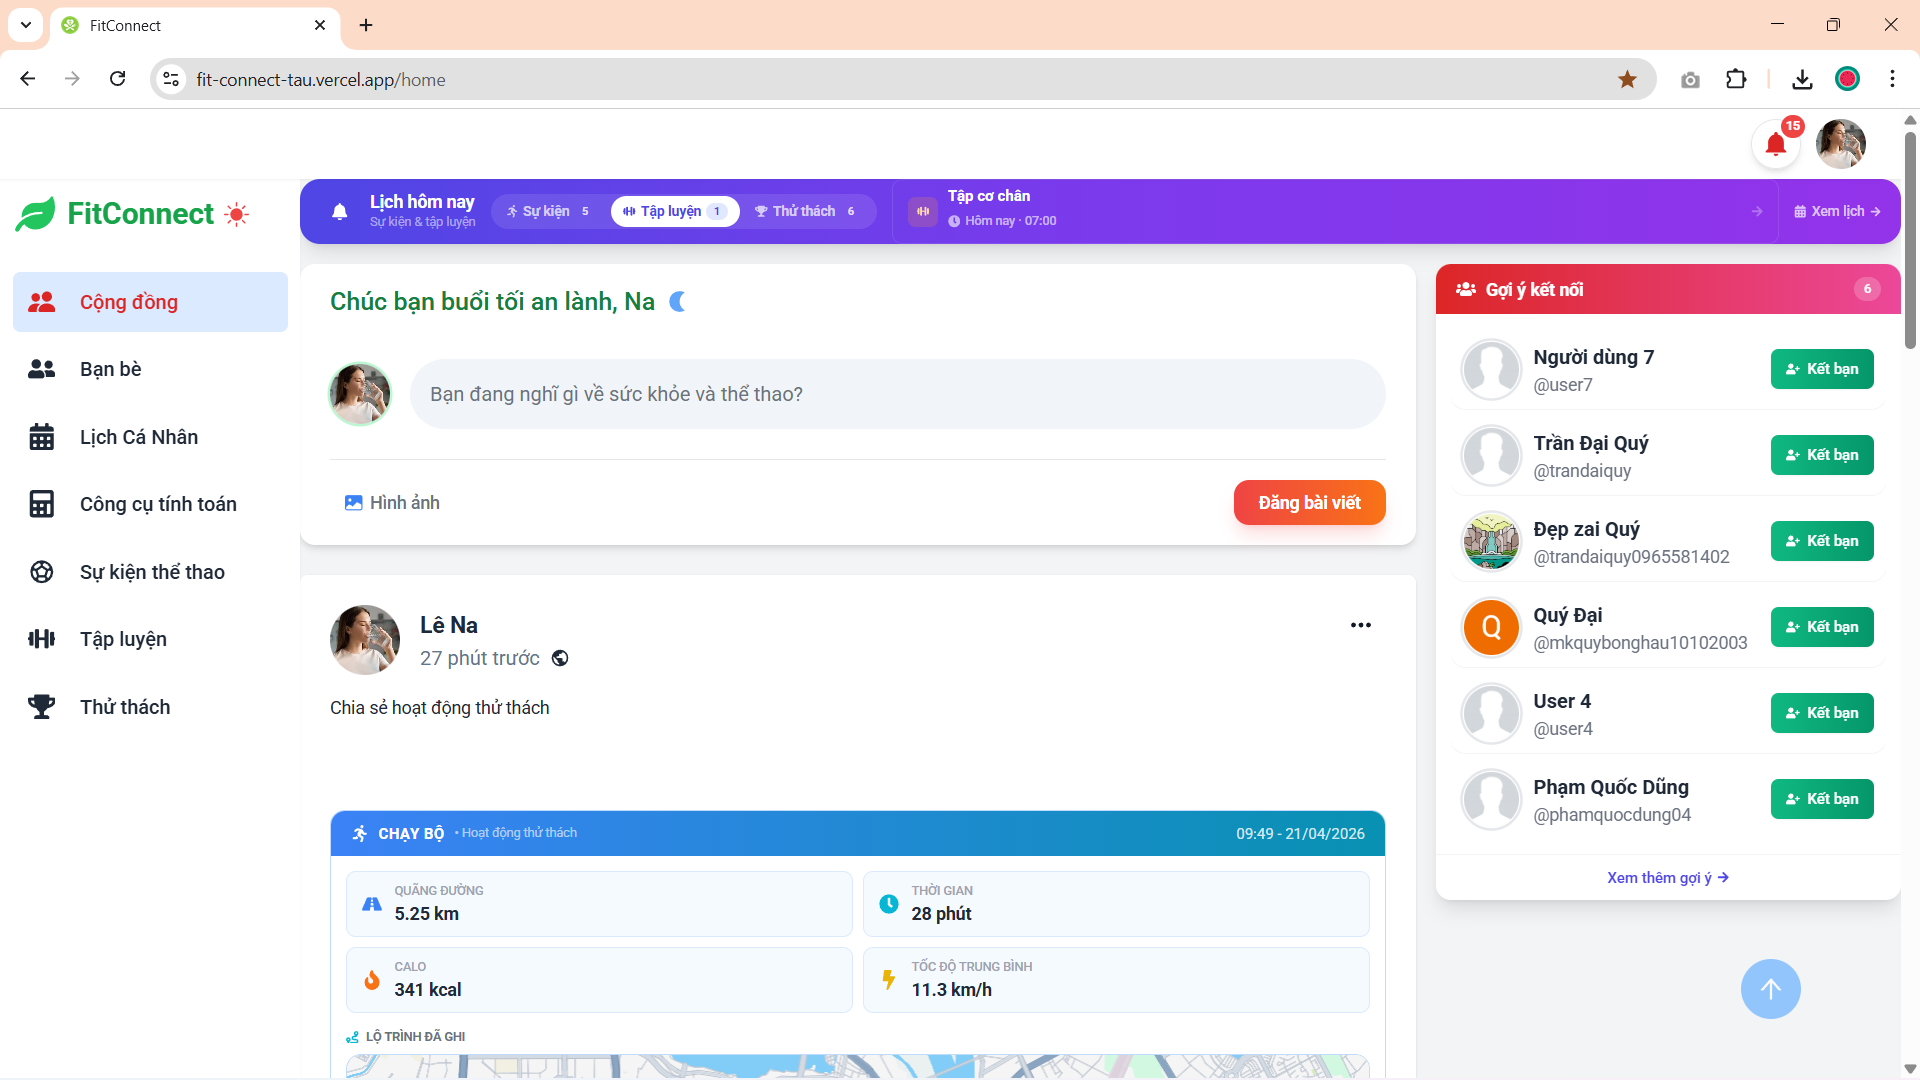
\includegraphics[width=\textwidth]{Images/IMG/nhom8/lichhomnaytapluyen.png}
        \caption{Người dùng theo dõi lịch tập luyện trong ngày hiện tại}
        \label{fig:impl_cal_today_workout}
    \end{subfigure}
\end{figure}

\end{itemize}

\subsubsection{Luồng thao tác trên trung tâm Thông báo}
\begin{itemize}
    \item Từ biểu tượng chuông, người dùng mở trung tâm thông báo với ba tab: \textbf{Tất cả} (tổng hợp toàn bộ), \textbf{Tương tác} (kết bạn, mời tham gia, bình luận) và \textbf{Hệ thống} (cảnh báo/cập nhật nền tảng). Người dùng có thể đánh dấu đã đọc, xóa thông báo và nhấn để điều hướng nhanh đến nội dung liên quan.

\begin{figure}[H]
    \centering
    \begin{subfigure}[b]{0.30\textwidth}
        \centering
        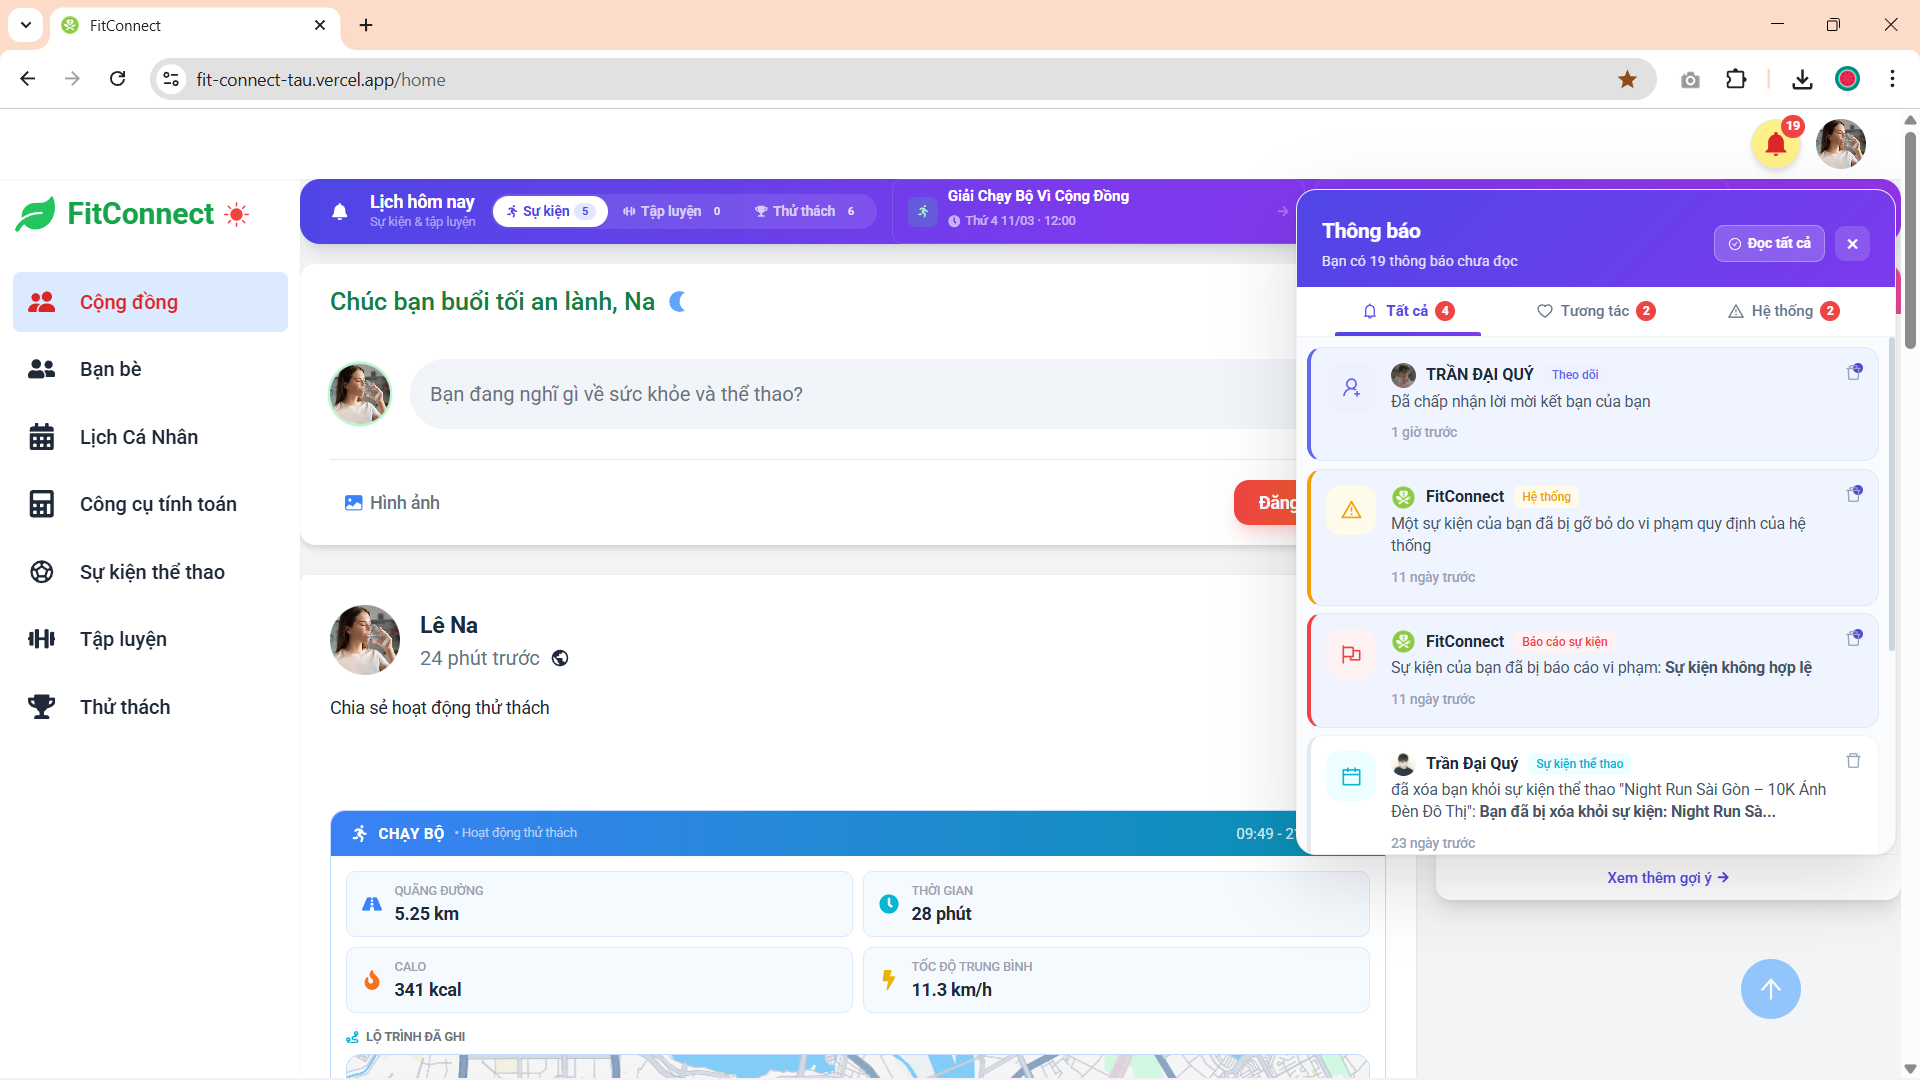
\includegraphics[width=\textwidth]{Images/IMG/nhom8/thongbaotatca.png}
        \caption{Tab Tất cả}
        \label{fig:impl_noti_all}
    \end{subfigure}
    \hfill
    \begin{subfigure}[b]{0.30\textwidth}
        \centering
        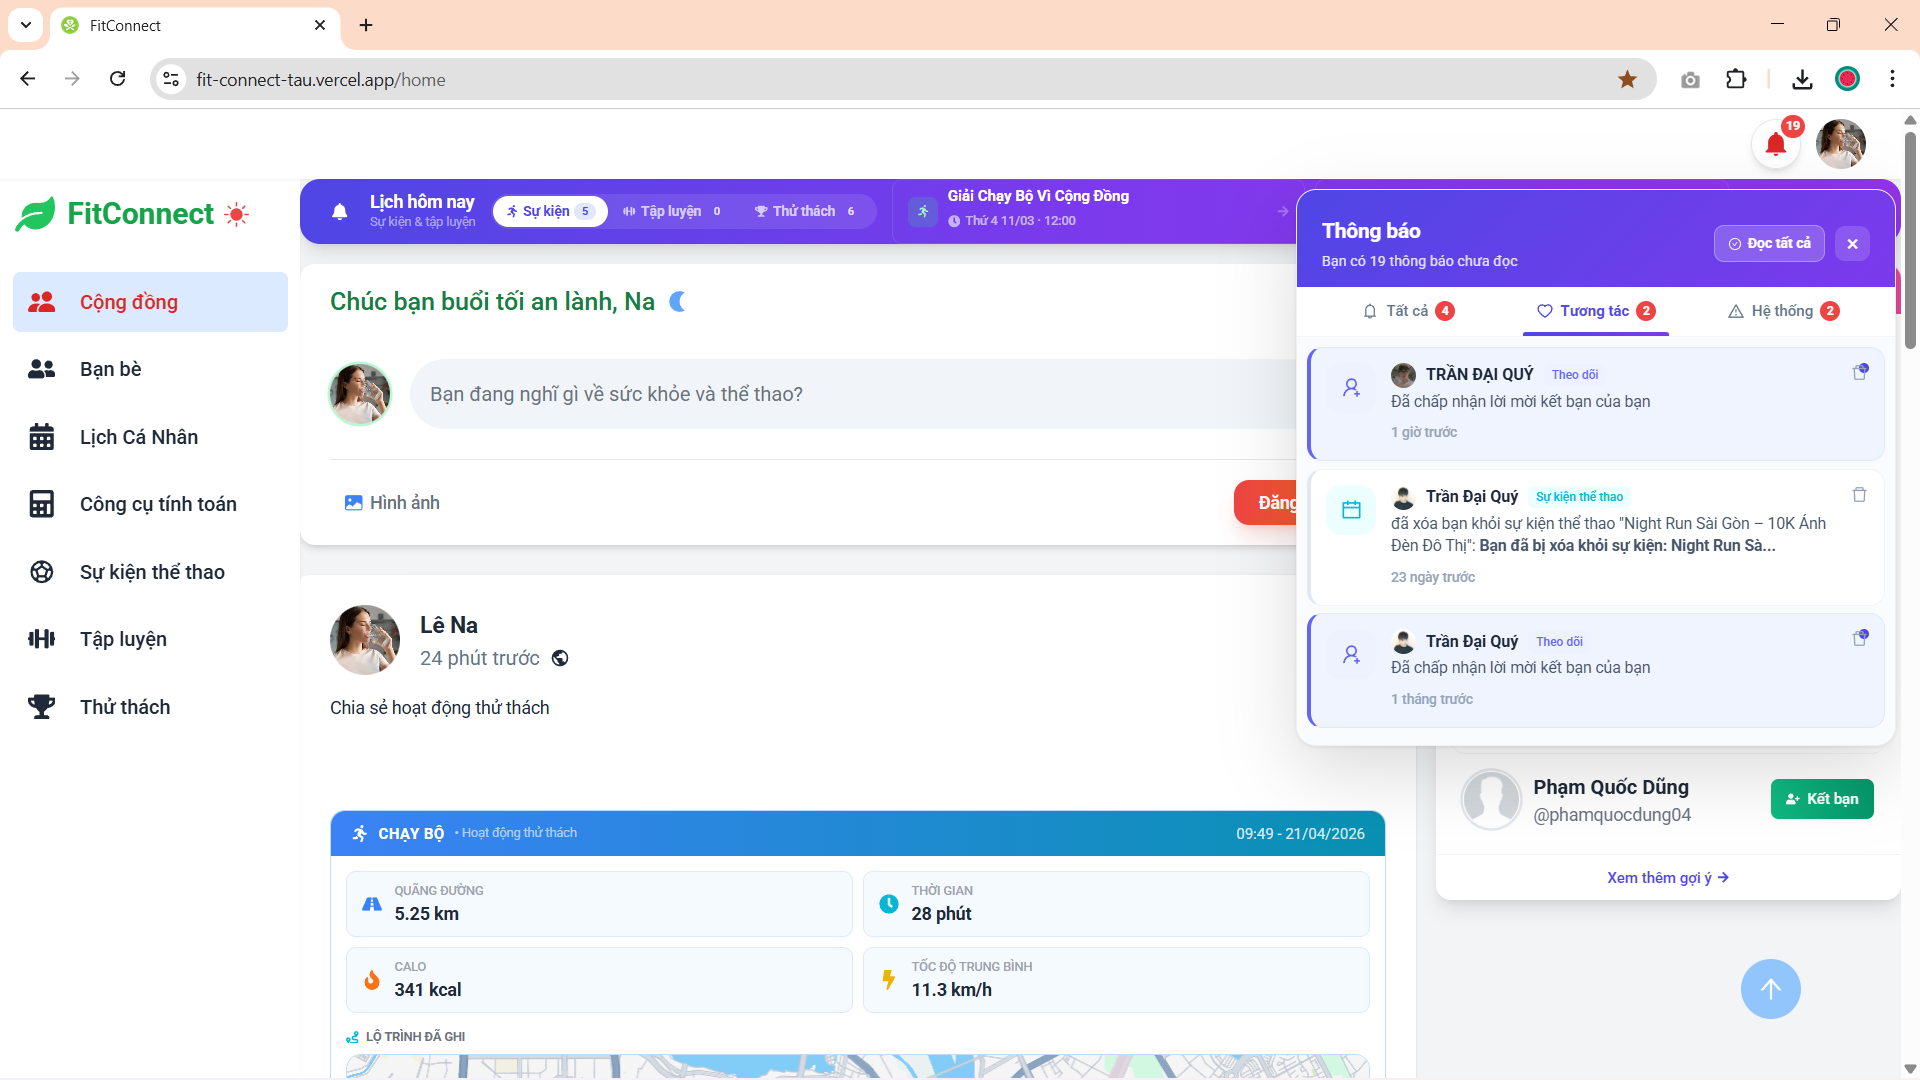
\includegraphics[width=\textwidth]{Images/IMG/nhom8/thongbaotuongtac.png}
        \caption{Tab Tương tác}
        \label{fig:impl_noti_social}
    \end{subfigure}
    \hfill
    \begin{subfigure}[b]{0.30\textwidth}
        \centering
        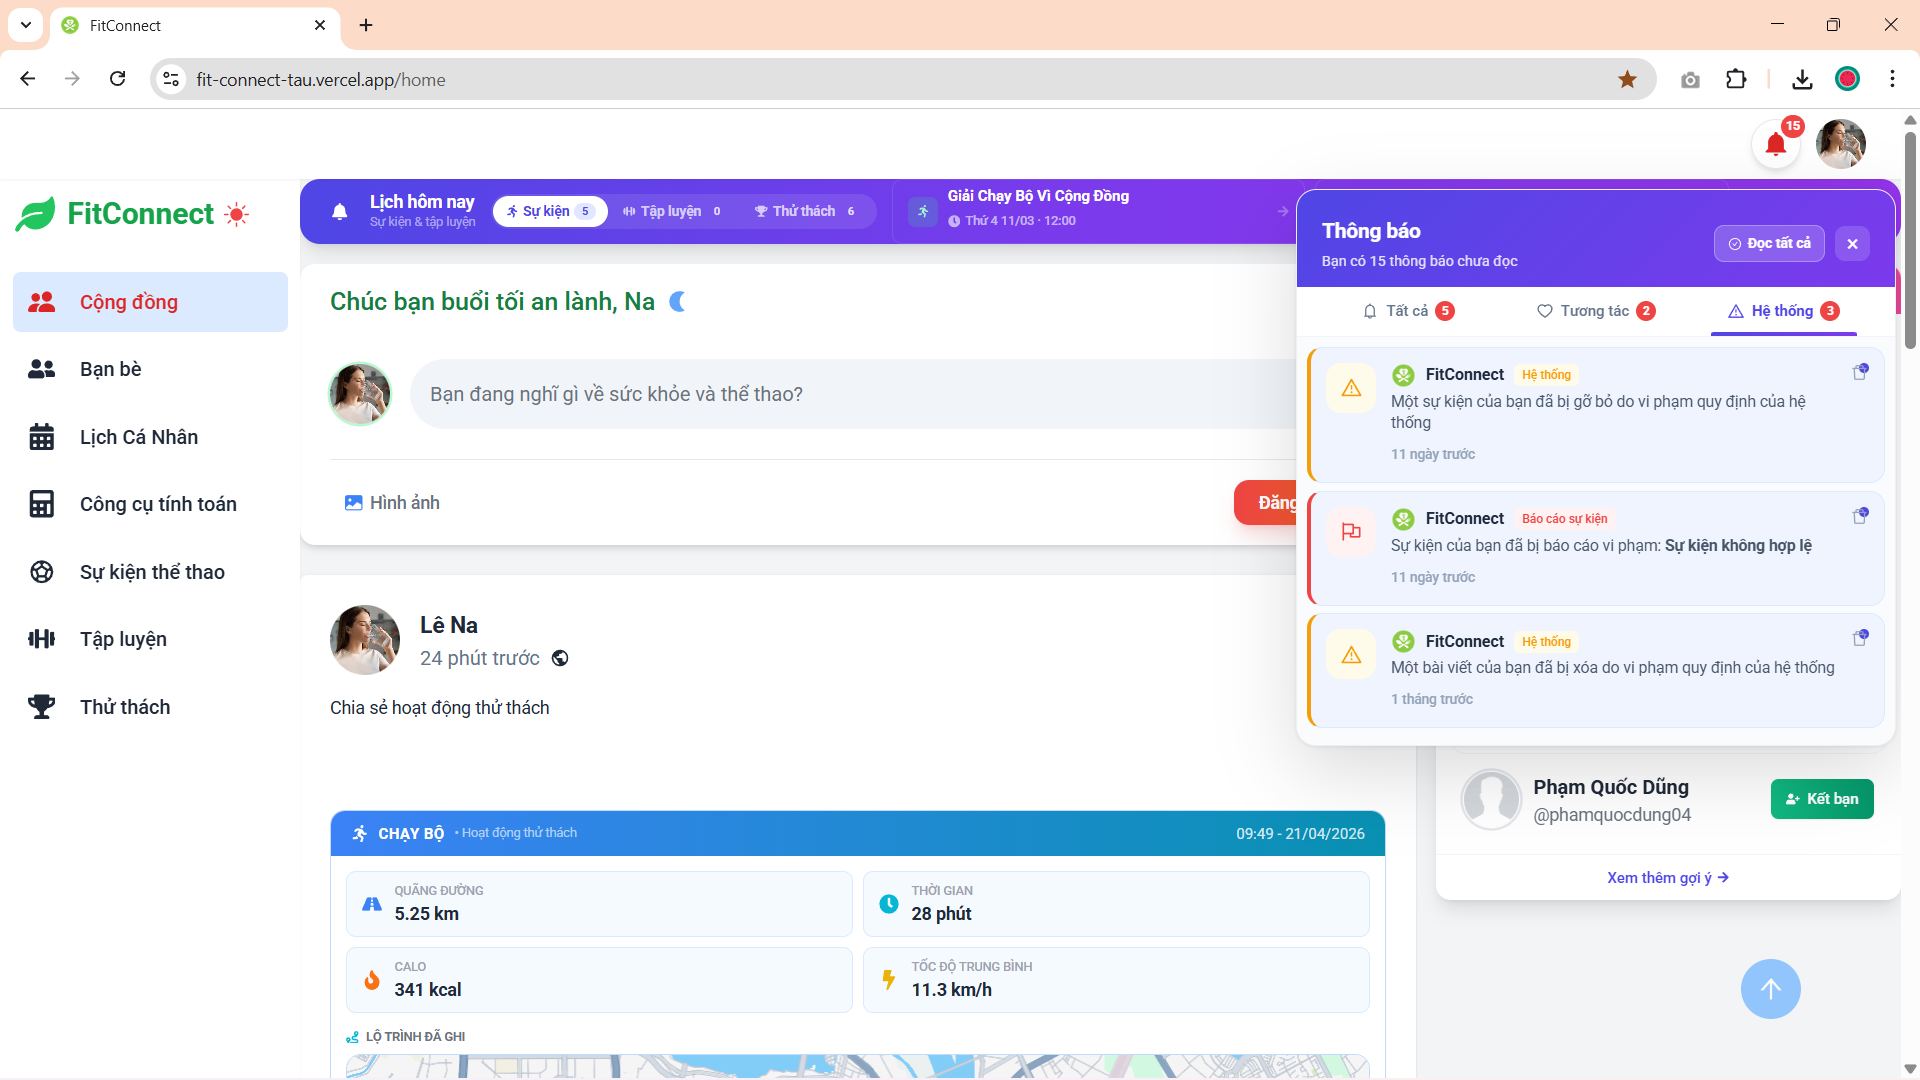
\includegraphics[width=\textwidth]{Images/IMG/nhom8/thongbaohethong.png}
        \caption{Tab Hệ thống}
        \label{fig:impl_noti_system}
    \end{subfigure}
    \vspace{0.3em}
    \caption{Trung tâm Thông báo với ba tab phân loại theo ngữ cảnh}
    \label{fig:impl_noti_center}
\end{figure}

\end{itemize}

\subsection{Nhóm tính năng Bạn bè}
\label{subsec:impl_friends}

Nhóm tính năng Bạn bè giúp người dùng xây dựng mạng lưới kết nối trong hệ thống, quản lý quan hệ theo dõi hai chiều và tăng tương tác thông qua lời mời tham gia hoạt động. Cơ chế cốt lõi của nhóm này dựa trên mô hình follow: khi hai người dùng theo dõi lẫn nhau thì được xem là bạn bè. Hệ thống đồng thời cung cấp danh sách gợi ý để người dùng mở rộng kết nối, kèm các thông báo thời gian thực cho những hành động quan trọng như gửi lời mời, chấp nhận kết bạn, và mời tham gia sự kiện/thử thách.

\subsubsection{Luồng thao tác quản lý bạn bè}
\begin{itemize}
    \item Người dùng truy cập trang Bạn bè, hệ thống hiển thị dashboard quản lý quan hệ gồm các khu vực chính: danh sách Bạn bè, Lời mời kết bạn, Người bạn theo dõi, Người theo dõi bạn, và khu vực Khám phá bạn bè để gợi ý kết nối mới.

\begin{figure}[H]
    \centering
    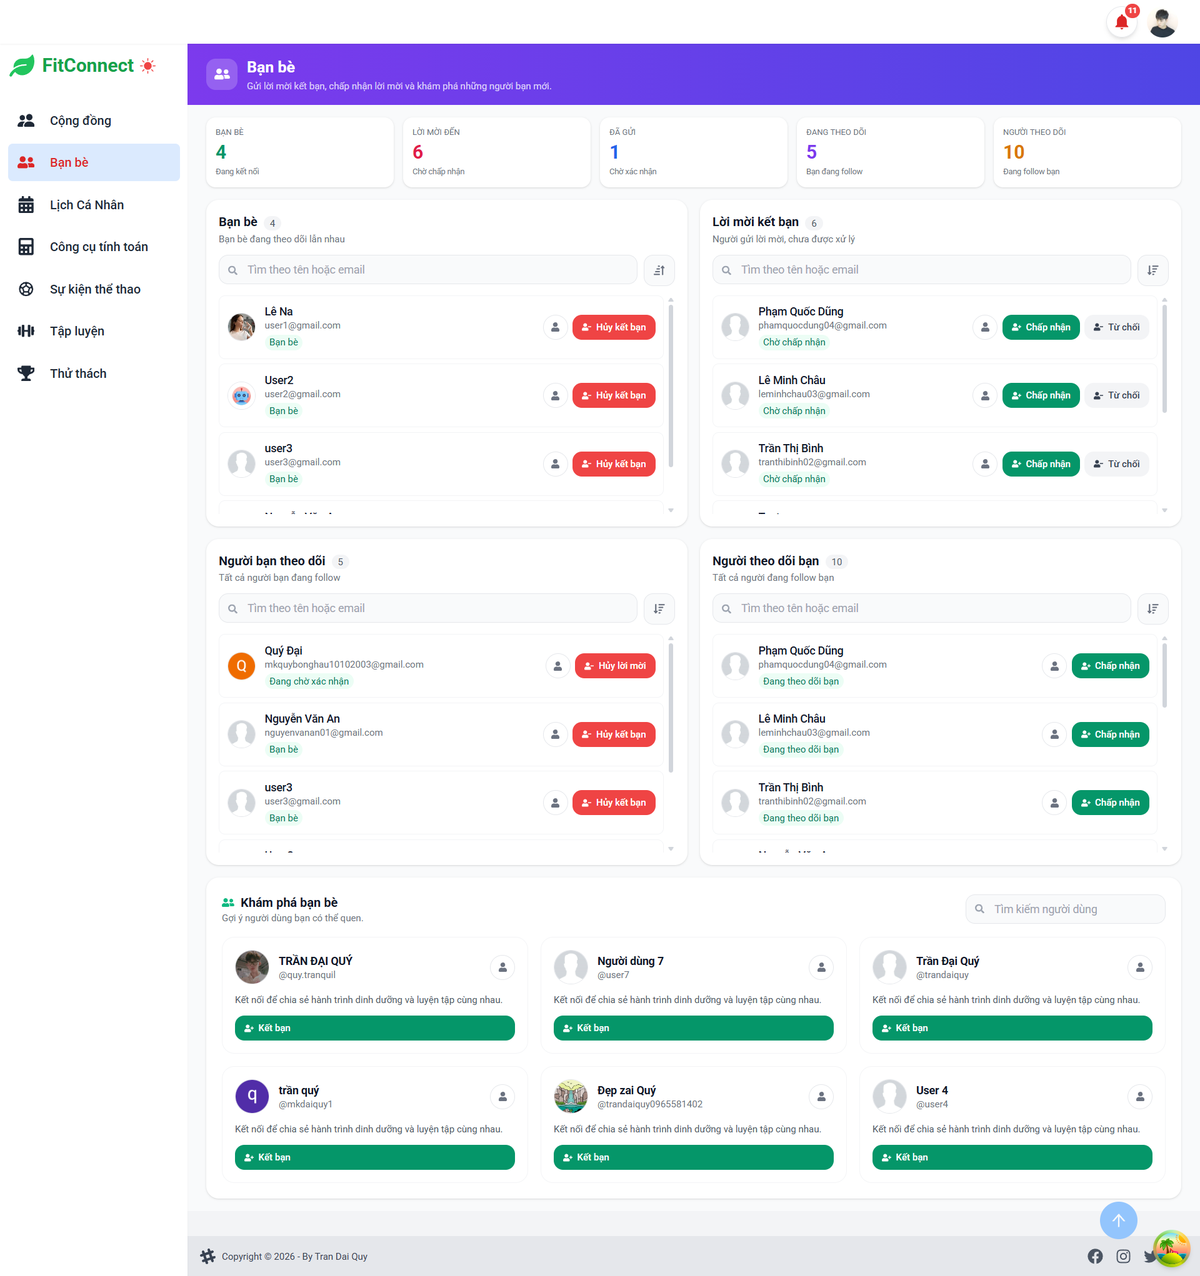
\includegraphics[width=0.60\textwidth]{Images/IMG/Nhom7/danhsachbanbe.png}
    \caption{Hệ thống hiển thị trang quản lý bạn bè với các danh sách quan hệ}
    \label{fig:impl_fr_dashboard}
\end{figure}


    \item Tại khu vực Lời mời kết bạn, người dùng có thể nhấn ``Chấp nhận'' để xác nhận lời mời. Sau khi chấp nhận, quan hệ giữa hai tài khoản chuyển thành bạn bè (theo dõi hai chiều), đồng thời hệ thống cập nhật số liệu thống kê liên quan trên trang.

\begin{figure}[H]
    \centering
    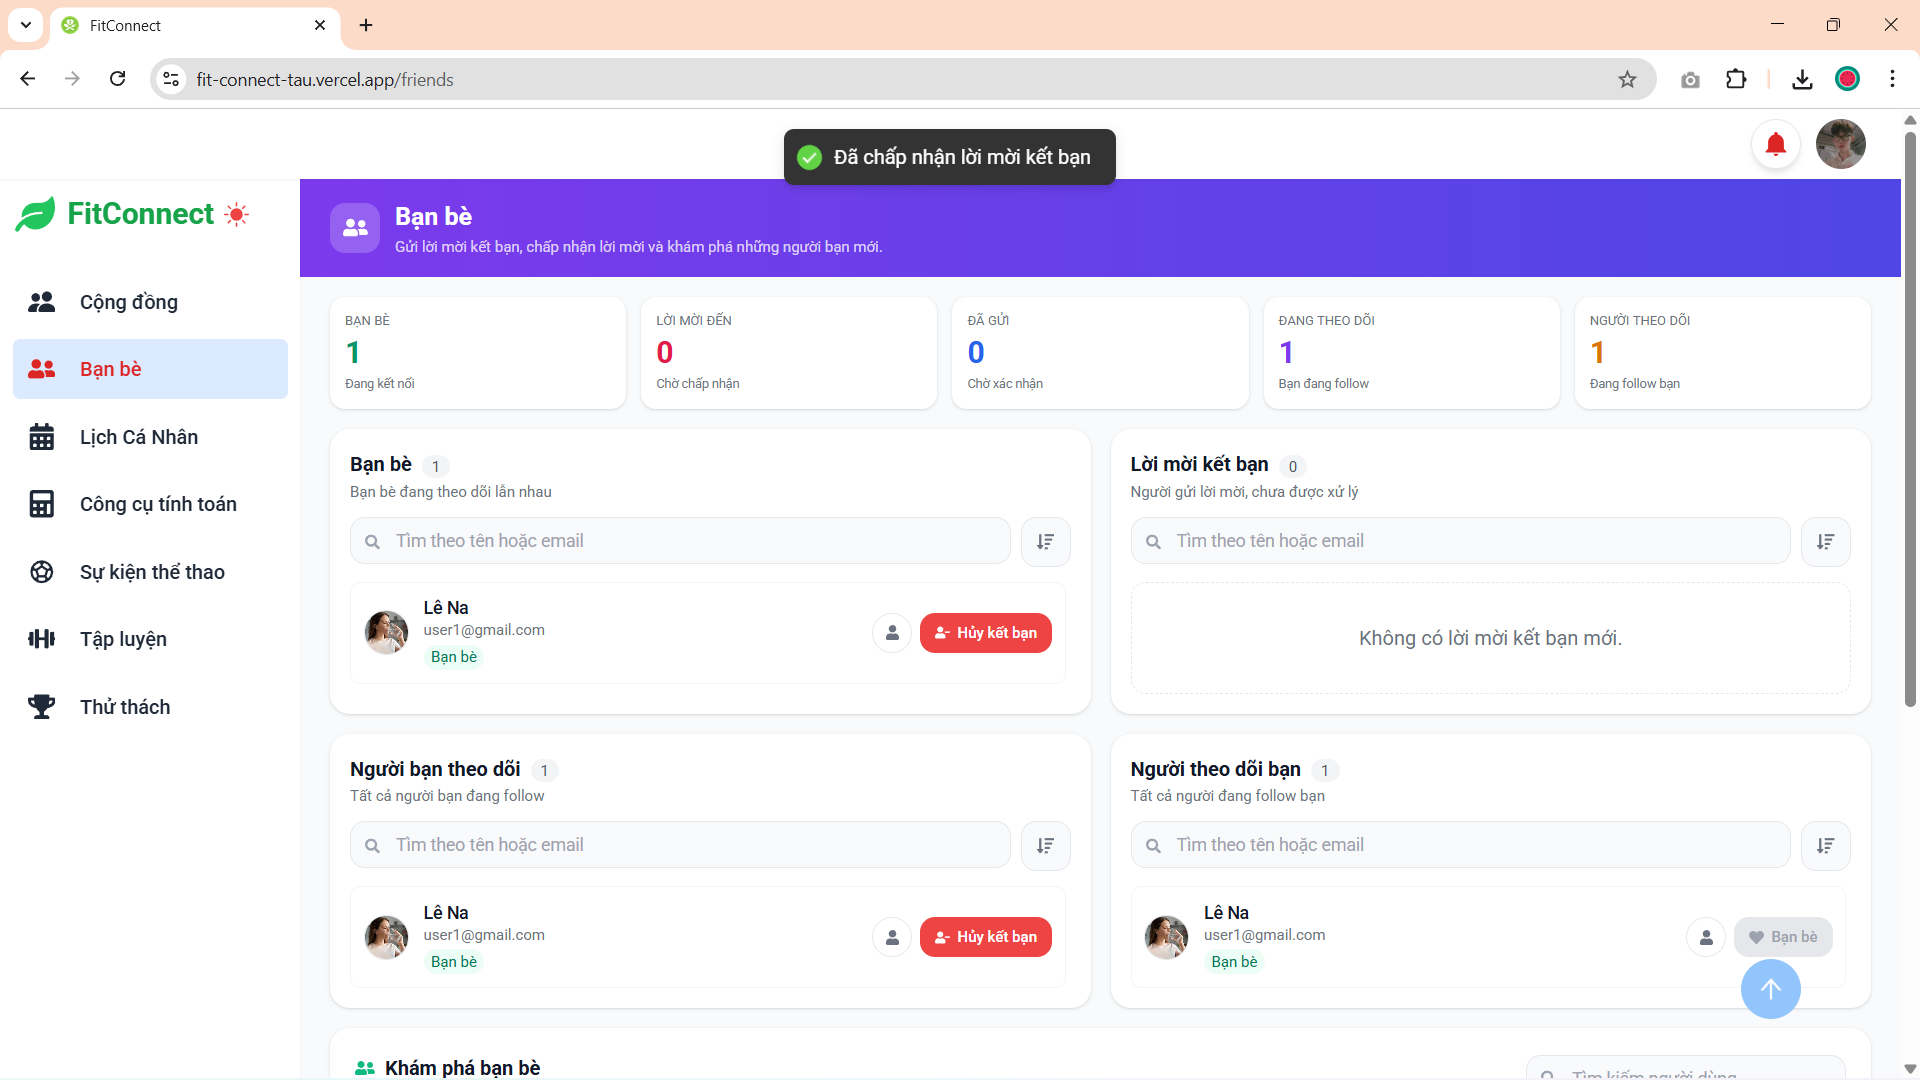
\includegraphics[width=0.60\textwidth]{Images/IMG/Nhom7/chapnhanketban.png}
    \caption{Người dùng thao tác chấp nhận lời mời kết bạn}
    \label{fig:impl_fr_accept}
\end{figure}


    \item Khi một người dùng gửi lời mời kết bạn, phía người nhận sẽ thấy thông báo tương ứng trong trung tâm thông báo. Người nhận có thể nhấn vào thông báo để điều hướng tới trang quản lý bạn bè và thực hiện xử lý lời mời.

\begin{figure}[H]
    \centering
    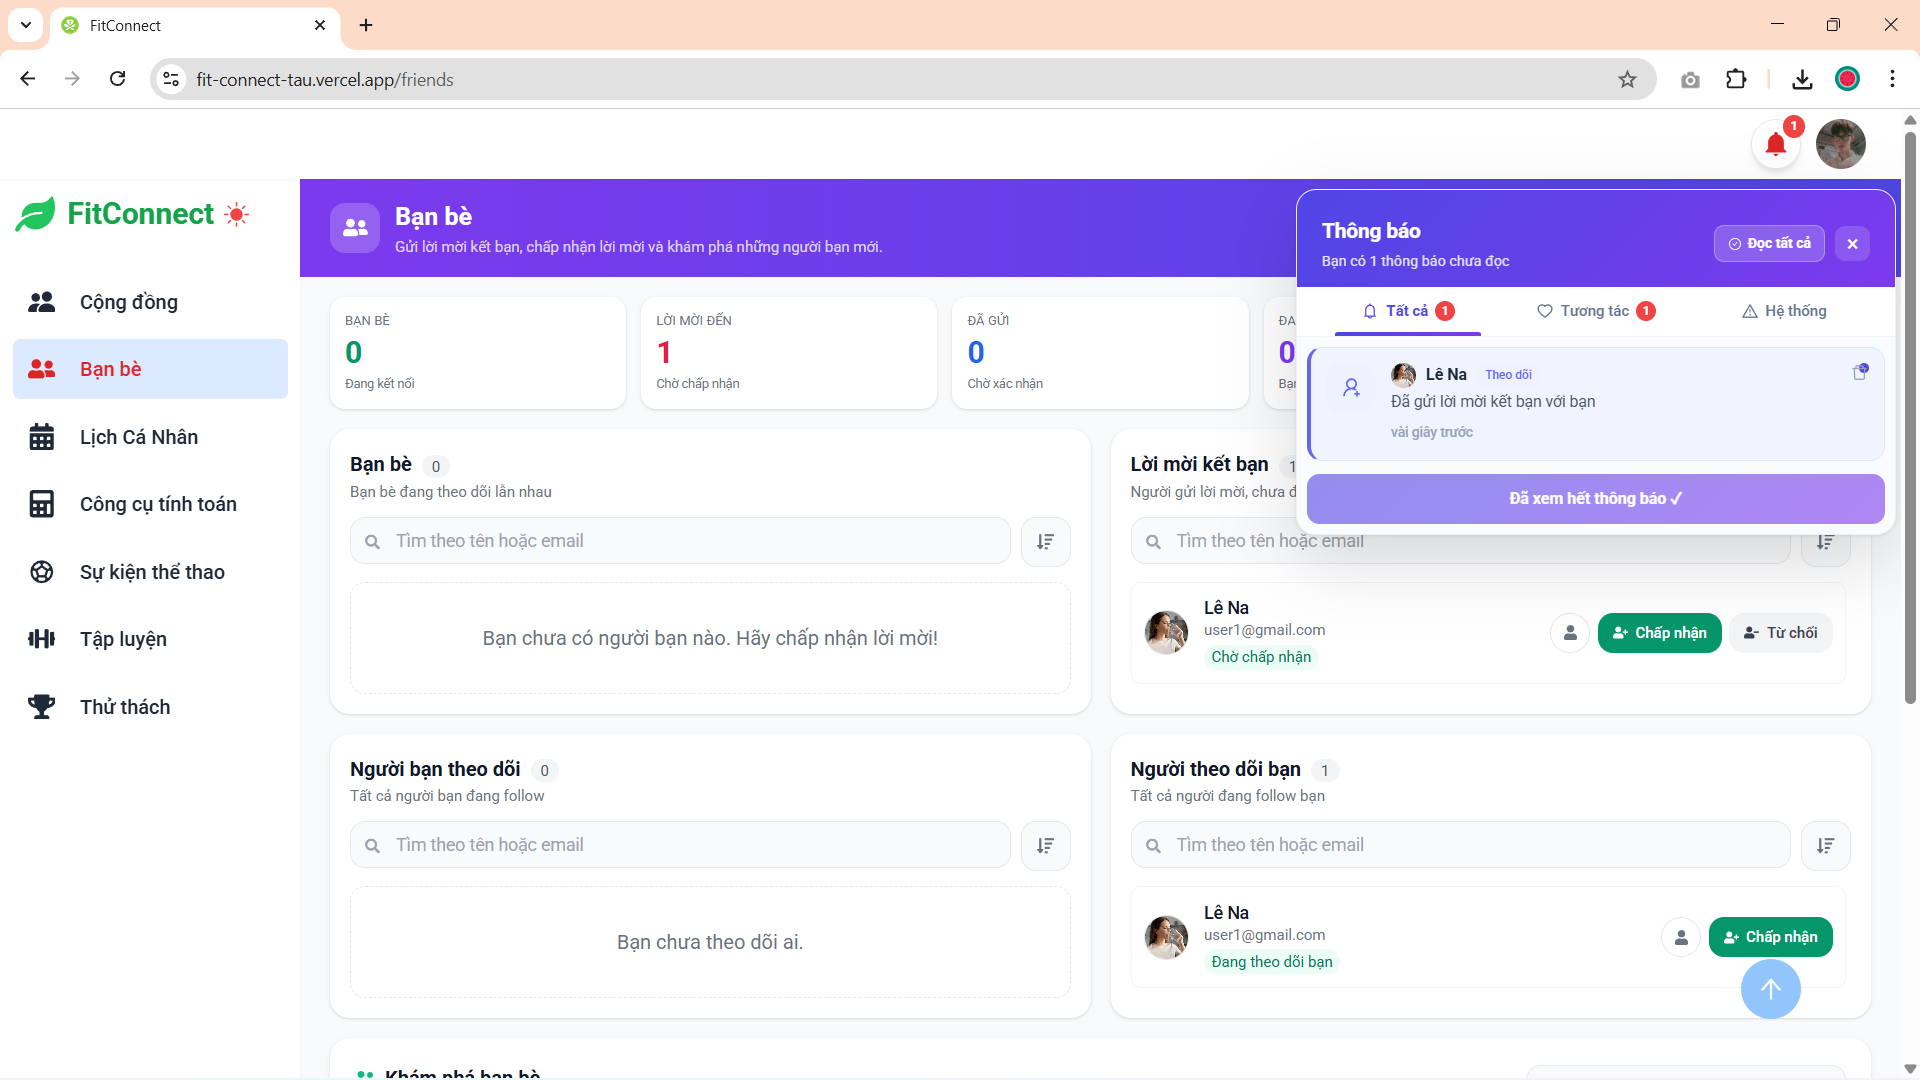
\includegraphics[width=0.60\textwidth]{Images/IMG/Nhom7/xemthongbaoguiketbanchominh.png}
    \caption{Người dùng nhận thông báo có lời mời kết bạn mới}
    \label{fig:impl_fr_request_noti}
\end{figure}


    \item Sau khi lời mời được chấp nhận, người gửi nhận thông báo xác nhận hai tài khoản đã trở thành bạn bè, đảm bảo cả hai bên đều nắm được trạng thái kết nối.

\end{itemize}

\subsubsection{Luồng thao tác mời bạn bè tham gia hoạt động}
\begin{itemize}
    \item Người dùng có thể mời bạn bè tham gia sự kiện thể thao hoặc thử thách cộng đồng ngay tại giao diện chi tiết. Hệ thống hiển thị modal chọn bạn bè để gửi lời mời nhanh theo danh sách kết nối hiện có.

\begin{figure}[H]
    \centering
    \begin{subfigure}[b]{0.45\textwidth}
        \centering
        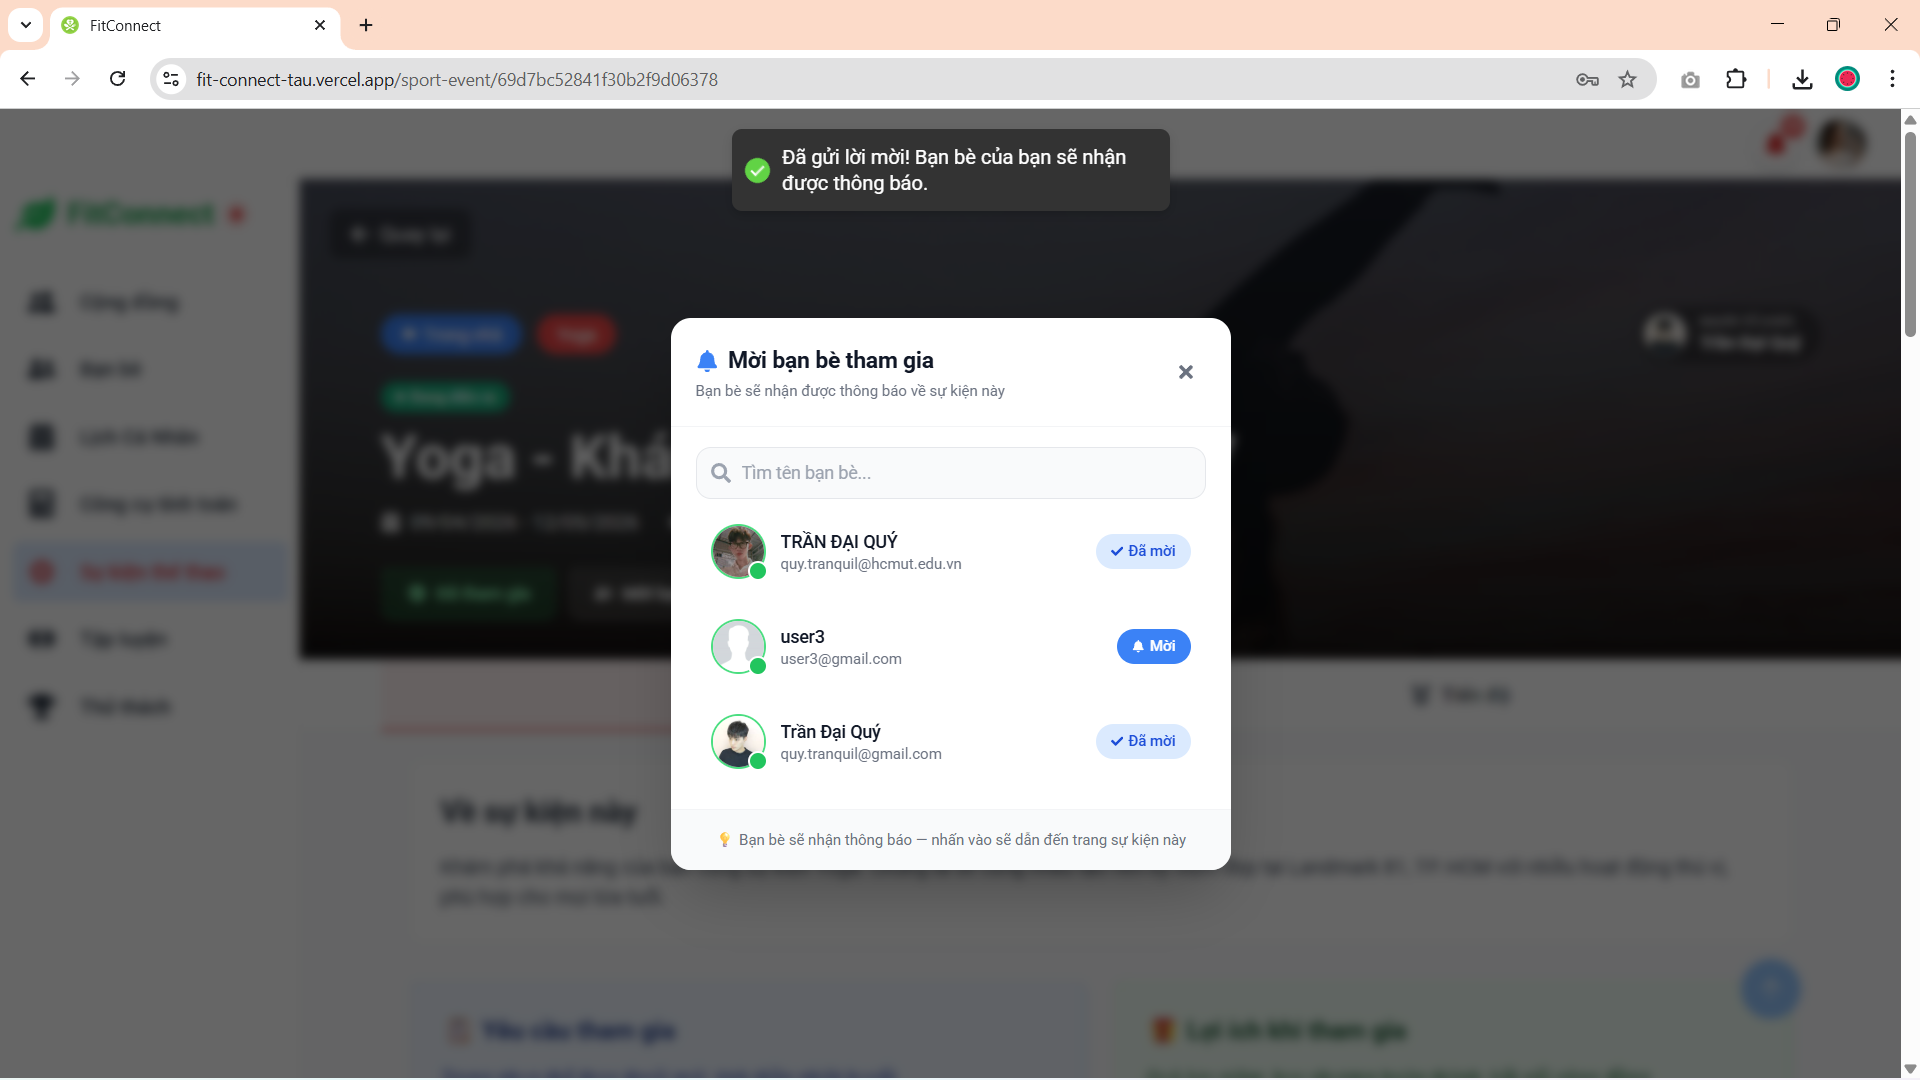
\includegraphics[width=\textwidth]{Images/IMG/Nhom7/moithamgiasukien.png}
        \caption{Mời bạn tham gia sự kiện}
        \label{fig:impl_fr_invite_event}
    \end{subfigure}
    \hfill
    \begin{subfigure}[b]{0.45\textwidth}
        \centering
        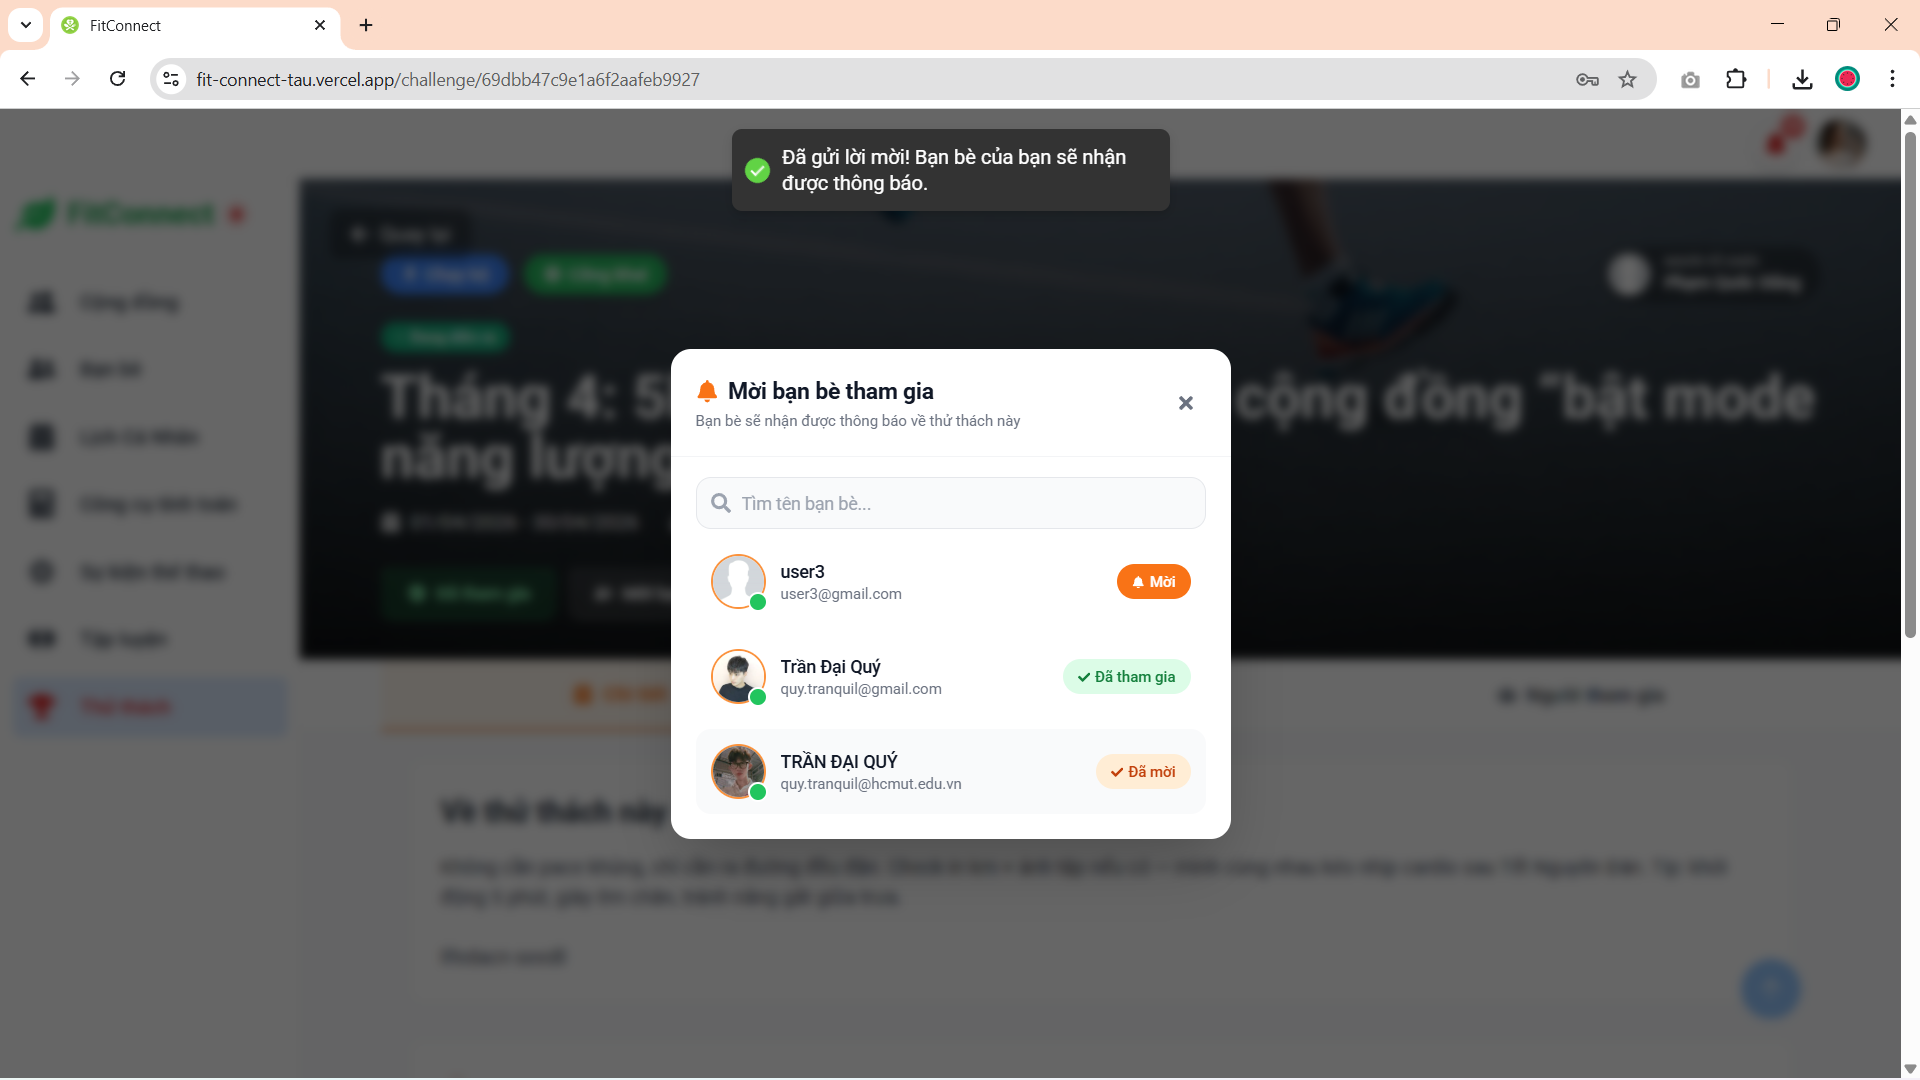
\includegraphics[width=\textwidth]{Images/IMG/Nhom7/moithamgiathuthach.png}
        \caption{Mời bạn tham gia thử thách}
        \label{fig:impl_fr_invite_challenge}
    \end{subfigure}
    \vspace{0.3em}
    \caption{Người dùng mời bạn bè tham gia hoạt động từ giao diện chi tiết}
    \label{fig:impl_fr_invite}
\end{figure}


    \item Khi được mời tham gia sự kiện hoặc thử thách, người dùng nhận thông báo lời mời trong hệ thống. Từ thông báo này, người dùng có thể truy cập nhanh nội dung được mời để xem chi tiết và quyết định tham gia.

\begin{figure}[H]
    \centering
    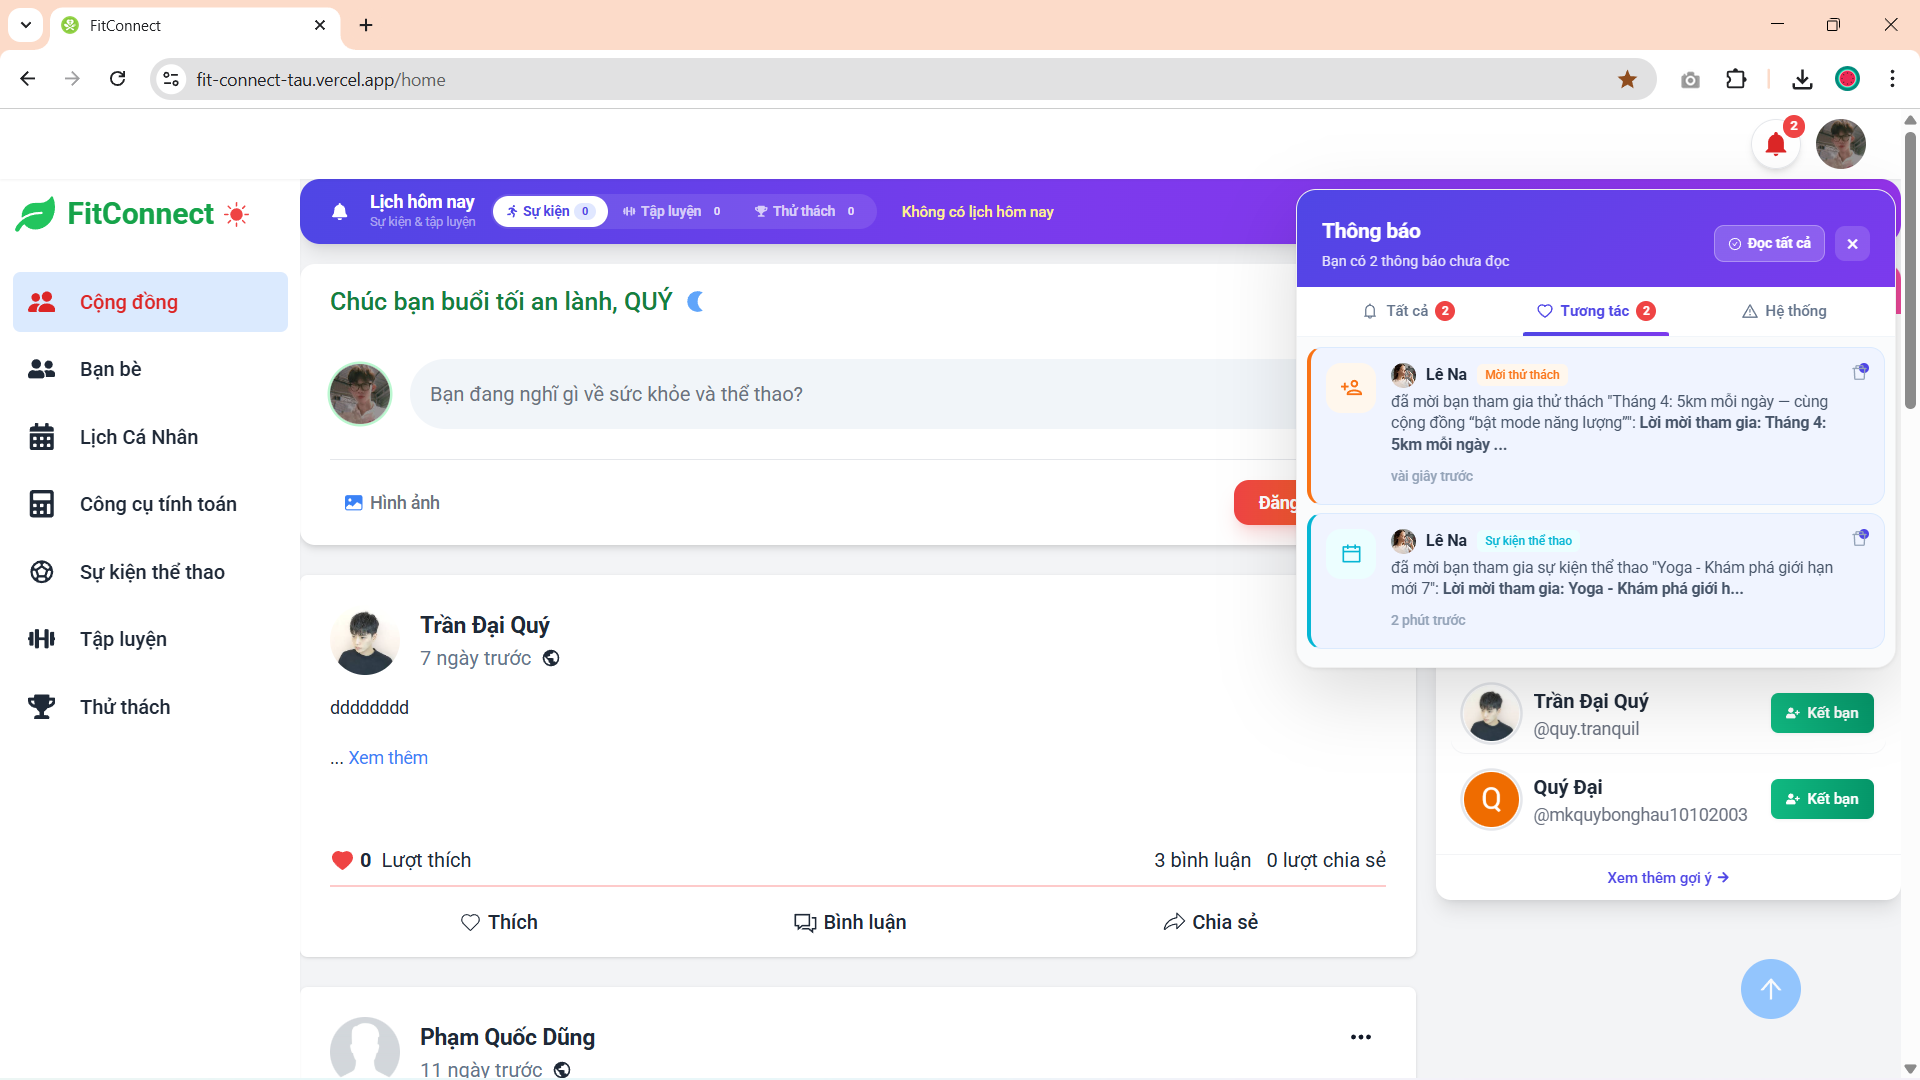
\includegraphics[width=0.60\textwidth]{Images/IMG/Nhom7/thongbaoloimoi.png}
    \caption{Hệ thống hiển thị thông báo lời mời tham gia hoạt động từ bạn bè}
    \label{fig:impl_fr_invite_noti}
\end{figure}

\end{itemize}

\subsection{Nhóm tính năng Quản trị hệ thống của Admin}
\label{subsec:impl_admin_system}

Nhóm tính năng Quản trị hệ thống là bộ công cụ dành riêng cho Quản trị viên (Admin) của nền tảng FitConnect, cung cấp khả năng giám sát toàn diện và điều hành tập trung các hoạt động trong hệ thống. Nhóm tính năng này bao gồm bốn trục nghiệp vụ cốt lõi: Giám sát Dashboard phân tích chuyên sâu, Quản trị người dùng và nhà kiểm duyệt, Kiểm duyệt nội dung đa tầng (bài viết, sự kiện, thử thách) và Quản lý hệ sinh thái dữ liệu (danh mục thể thao, thiết bị, kho bài tập). Giao diện Admin được xây dựng theo mô hình ``Hero-Stat'': mỗi trang quản lý gồm banner gradient chủ đề, thẻ thống kê tóm tắt và bảng dữ liệu mật độ cao nhằm tối ưu hóa trải nghiệm điều hành.

\subsubsection{Luồng thao tác giám sát tổng quan Dashboard}
\begin{itemize}
    \item Quản trị viên truy cập trang Dashboard, hệ thống hiển thị toàn cảnh bức tranh hoạt động thông qua các khối phân tích chuyên sâu. Tại phần \textbf{Tổng quan Hệ thống}, hệ thống cung cấp các thẻ số liệu cốt lõi (tài khoản, sự kiện, thử thách) với thiết kế trực quan giúp Admin nhanh chóng nắm bắt quy mô hiện tại của nền tảng.

\begin{figure}[H]
    \centering
    
\includegraphics[width=0.60\textwidth]{Images/IMG/nhom9/dashboard/dashboard.png}
    \caption{Trang Dashboard Tổng quan của Quản trị viên -- Toàn cảnh hệ thống}
    \label{fig:impl_admin_dashboard_overview}
\end{figure}


    \item Tại khối \textbf{Người dùng \& Sức khỏe}, hệ thống tự động phân tích và biểu đồ hóa dữ liệu nhân khẩu học (giới tính), mức độ tham gia hoạt động và phân bố chỉ số BMI của cộng đồng. Đồng thời, hệ thống còn vinh danh các cá nhân tích cực thông qua danh sách người dùng nổi bật.

    \item Đối với khối \textbf{Cộng đồng \& Sự kiện}, hệ thống theo dõi mức độ tăng trưởng thông qua biểu đồ xu hướng theo thời gian, giúp nhận diện sự kiện nào đang thu hút sự chú ý (phân loại sự kiện ngoài trời, trong nhà) và các môn thể thao phổ biến nhất trong cộng đồng.

    \item Tại khối \textbf{Thử thách}, Quản trị viên có thể giám sát hệ sinh thái thử thách thông qua các biểu đồ phân tích cơ cấu loại thử thách và phạm vi tham gia, từ đó có cái nhìn chi tiết về xu hướng rèn luyện sức khỏe của người dùng.
\end{itemize}

\subsubsection{Luồng thao tác quản lý người dùng}
\begin{itemize}
    \item Tại trang quản lý người dùng, hệ thống cung cấp một danh sách tổng hợp tất cả tài khoản với đầy đủ thông tin định danh và lịch sử vi phạm. Quản trị viên có thể sử dụng các công cụ tìm kiếm và sắp xếp để nhanh chóng truy xuất thông tin của bất kỳ người dùng nào trên hệ thống.

\begin{figure}[H]
    \centering
    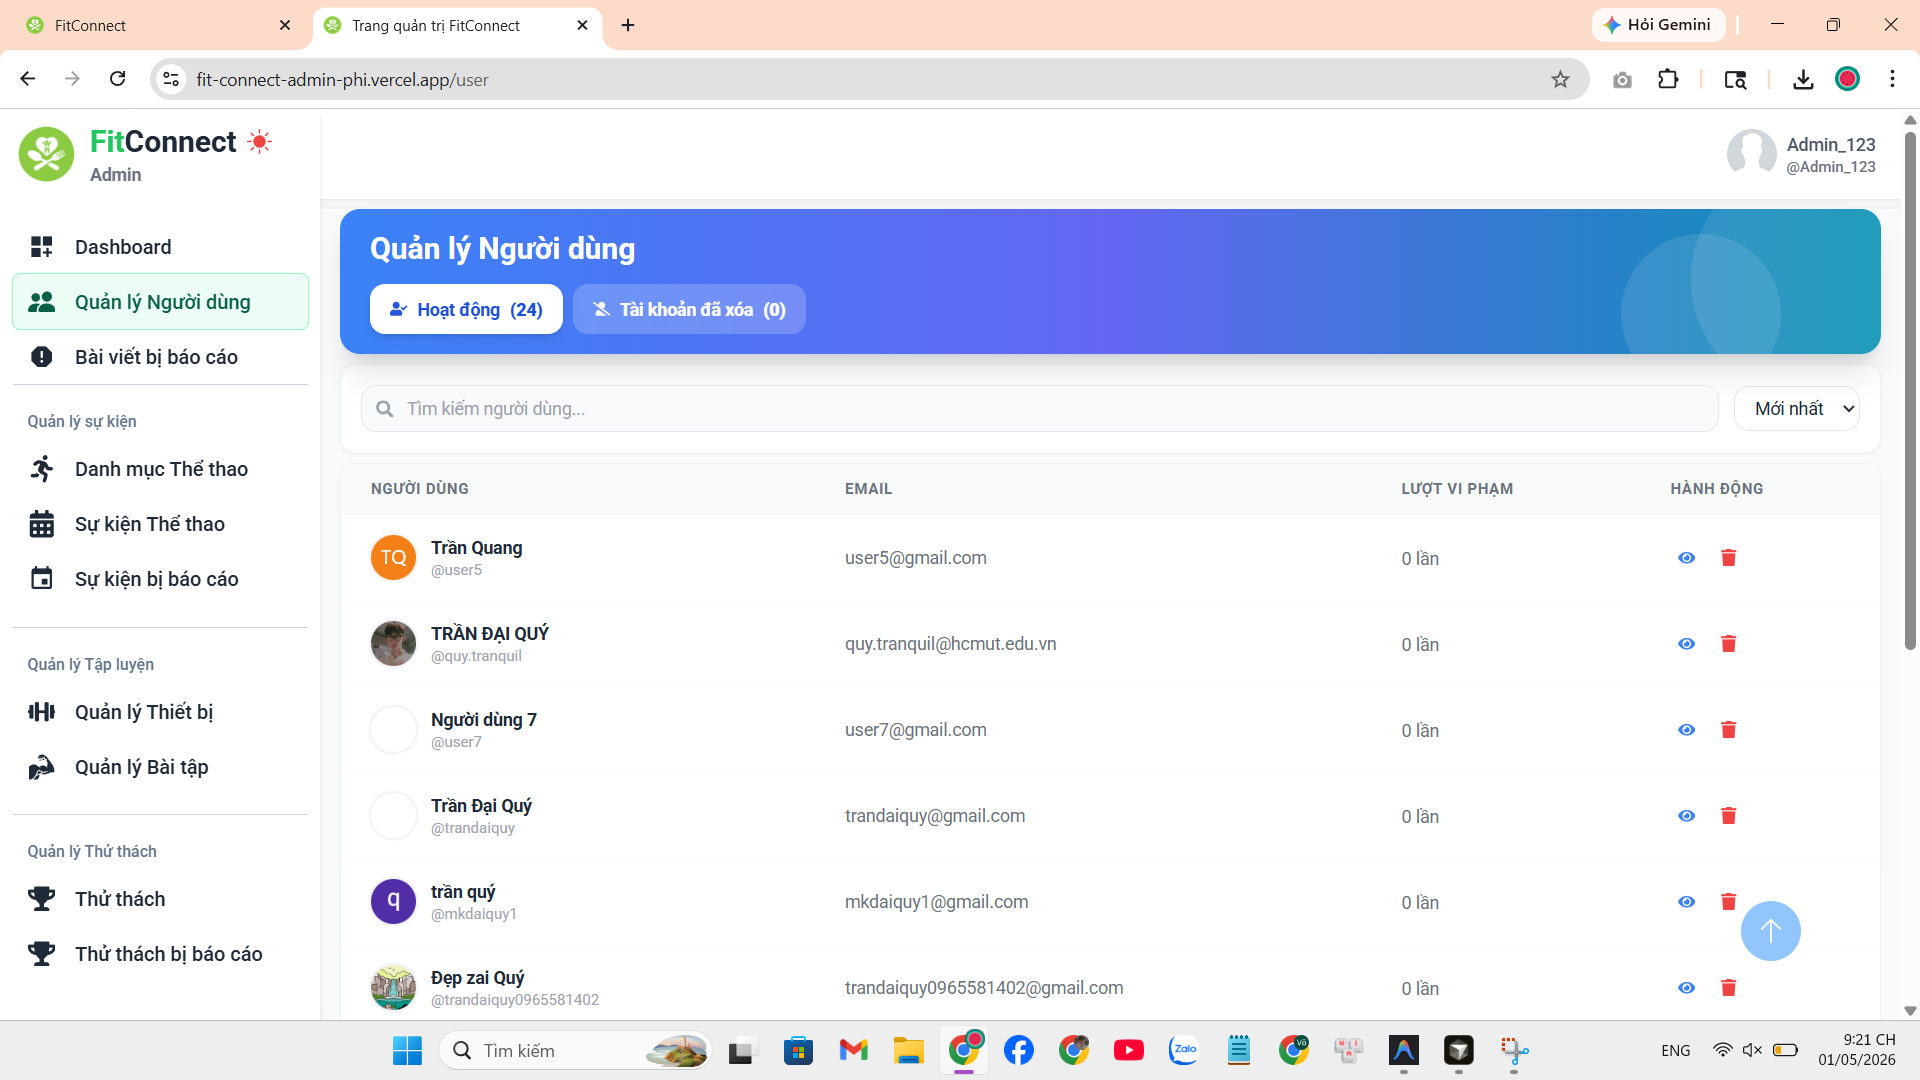
\includegraphics[width=0.60\textwidth]{Images/IMG/nhom9/quanlynguoidung/danhsachnguoidung.png}
    \caption{Quản trị viên xem danh sách người dùng đang hoạt động}
    \label{fig:impl_admin_user_list}
\end{figure}


    \item Để đánh giá mức độ tương tác, Admin có thể xem chi tiết hồ sơ hoạt động của từng cá nhân. Hệ thống sẽ mở ra một panel hiển thị chi tiết số liệu đóng góp của người đó trong cộng đồng cũng như tần suất tham gia sự kiện, thử thách.

\begin{figure}[H]
    \centering
    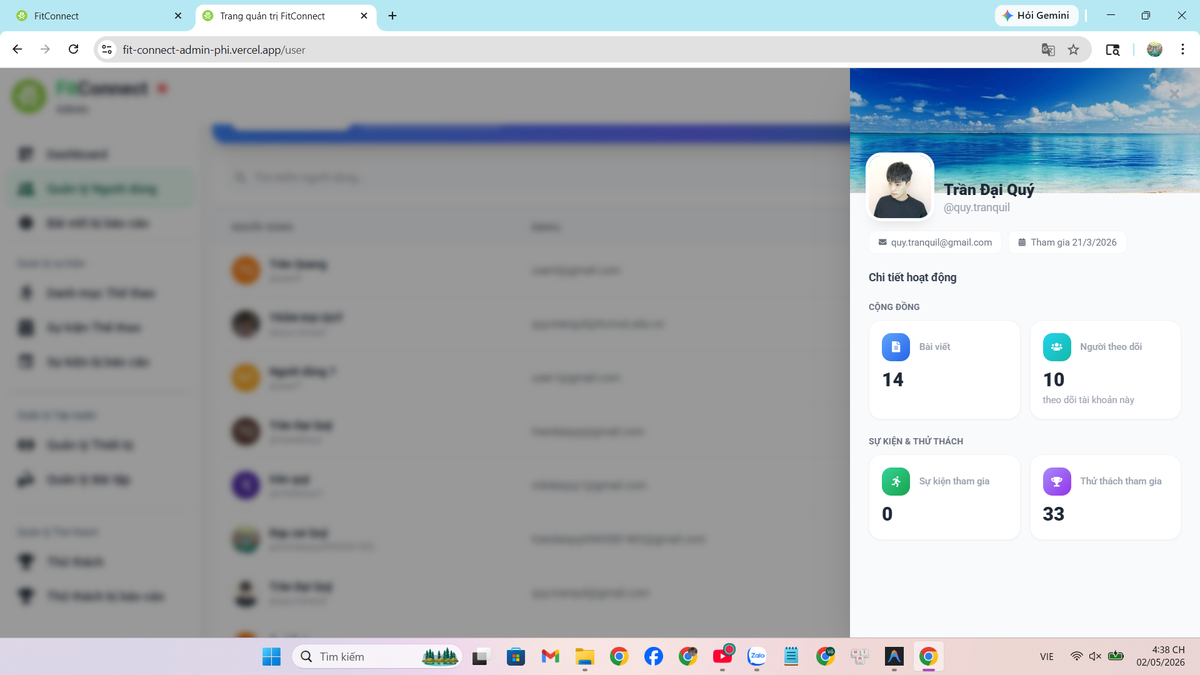
\includegraphics[width=0.60\textwidth]{Images/IMG/nhom9/quanlynguoidung/chitietnguoidung.png}
    \caption{Quản trị viên xem chi tiết hoạt động của người dùng}
    \label{fig:impl_admin_user_detail}
\end{figure}


    \item Khi phát hiện vi phạm, hệ thống hỗ trợ thao tác khóa tài khoản thông qua cơ chế xóa mềm (soft delete). Thao tác này yêu cầu xác nhận hai bước nhằm tránh rủi ro thao tác nhầm, đồng thời bảo toàn tính nguyên vẹn của dữ liệu lịch sử để phục vụ tra cứu sau này.

\begin{figure}[H]
    \centering
    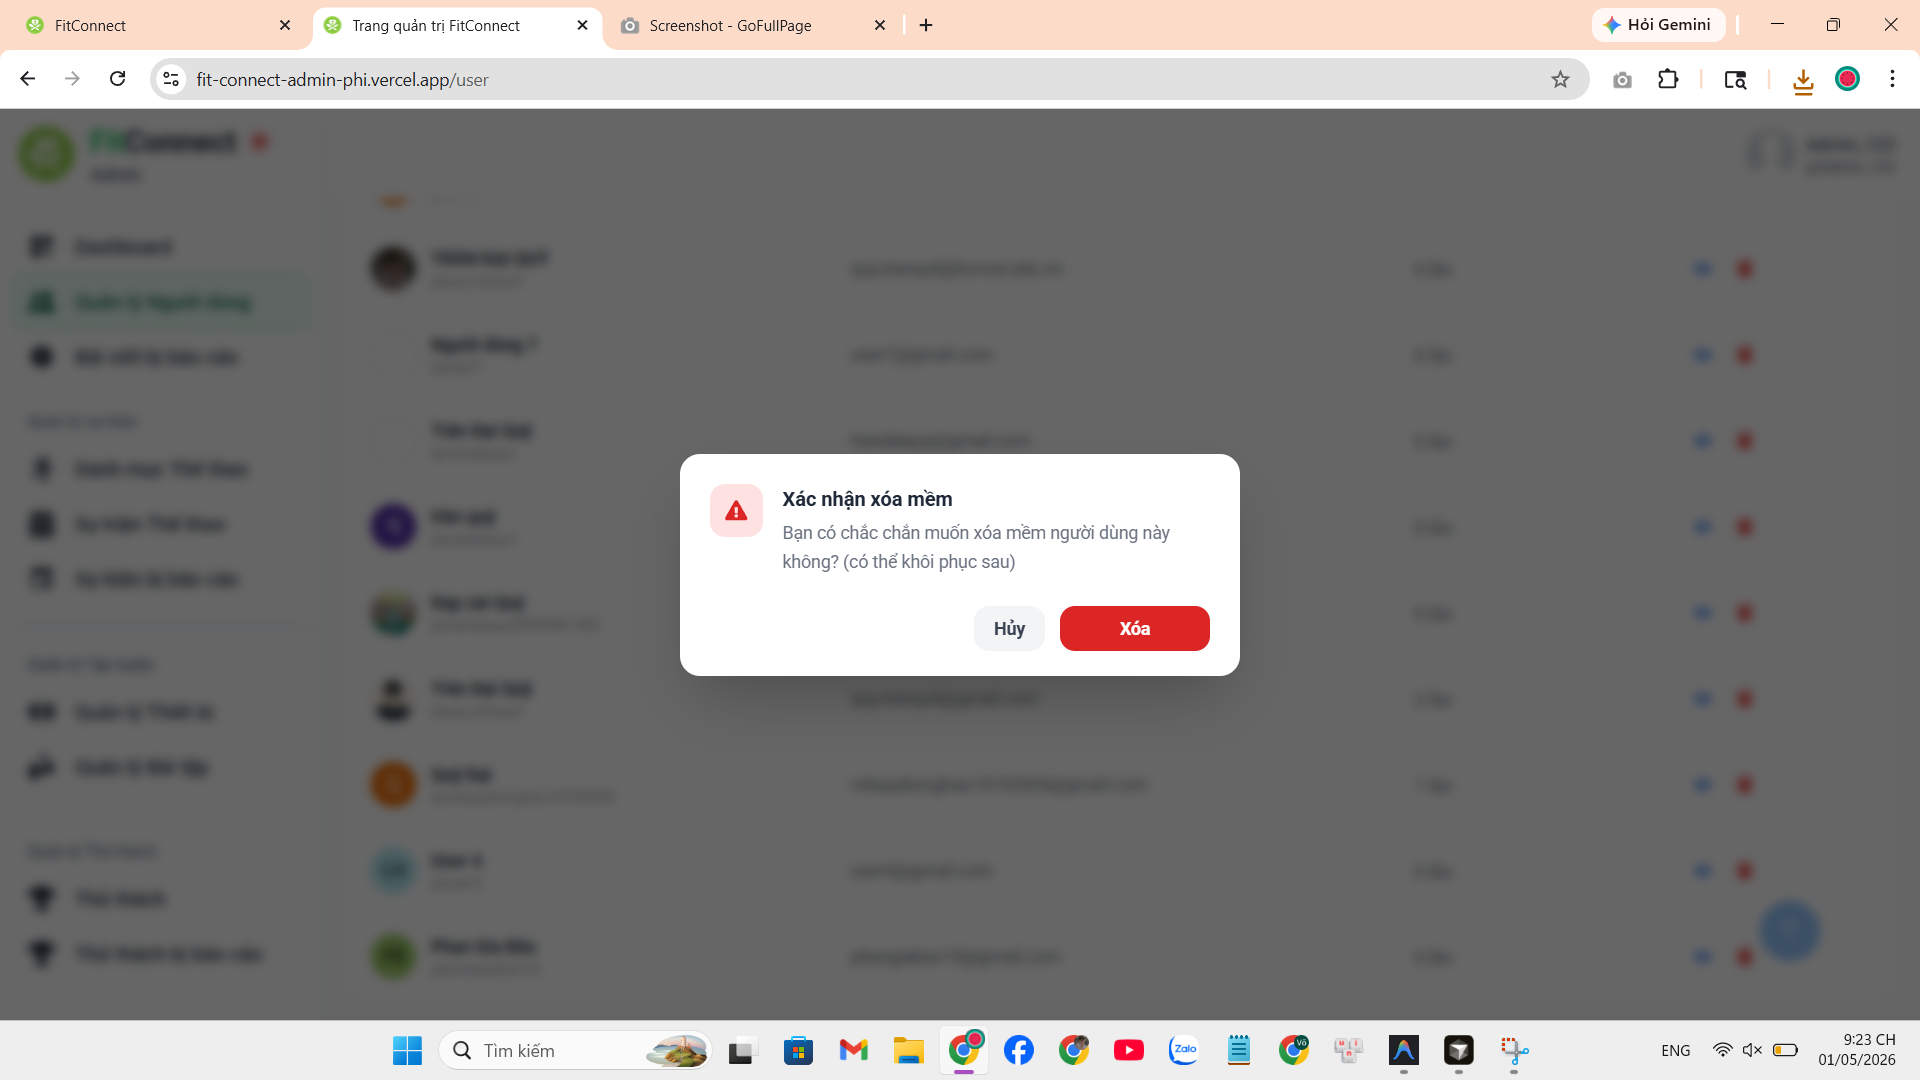
\includegraphics[width=0.60\textwidth]{Images/IMG/nhom9/quanlynguoidung/xoanguoidung.png}
    \caption{Hệ thống hiển thị hộp thoại xác nhận khóa tài khoản người dùng}
    \label{fig:impl_admin_user_delete_confirm}
\end{figure}


    \item Tài khoản vi phạm bị chuyển vào danh sách ``Đã xóa''; người dùng nhận thông báo lỗi xác thực khi đăng nhập. Hệ thống cho phép khôi phục tài khoản nếu xử lý sai lệch hoặc người dùng đã khắc phục vi phạm.

\begin{figure}[H]
    \centering
    \begin{subfigure}[b]{0.47\textwidth}
        \centering
        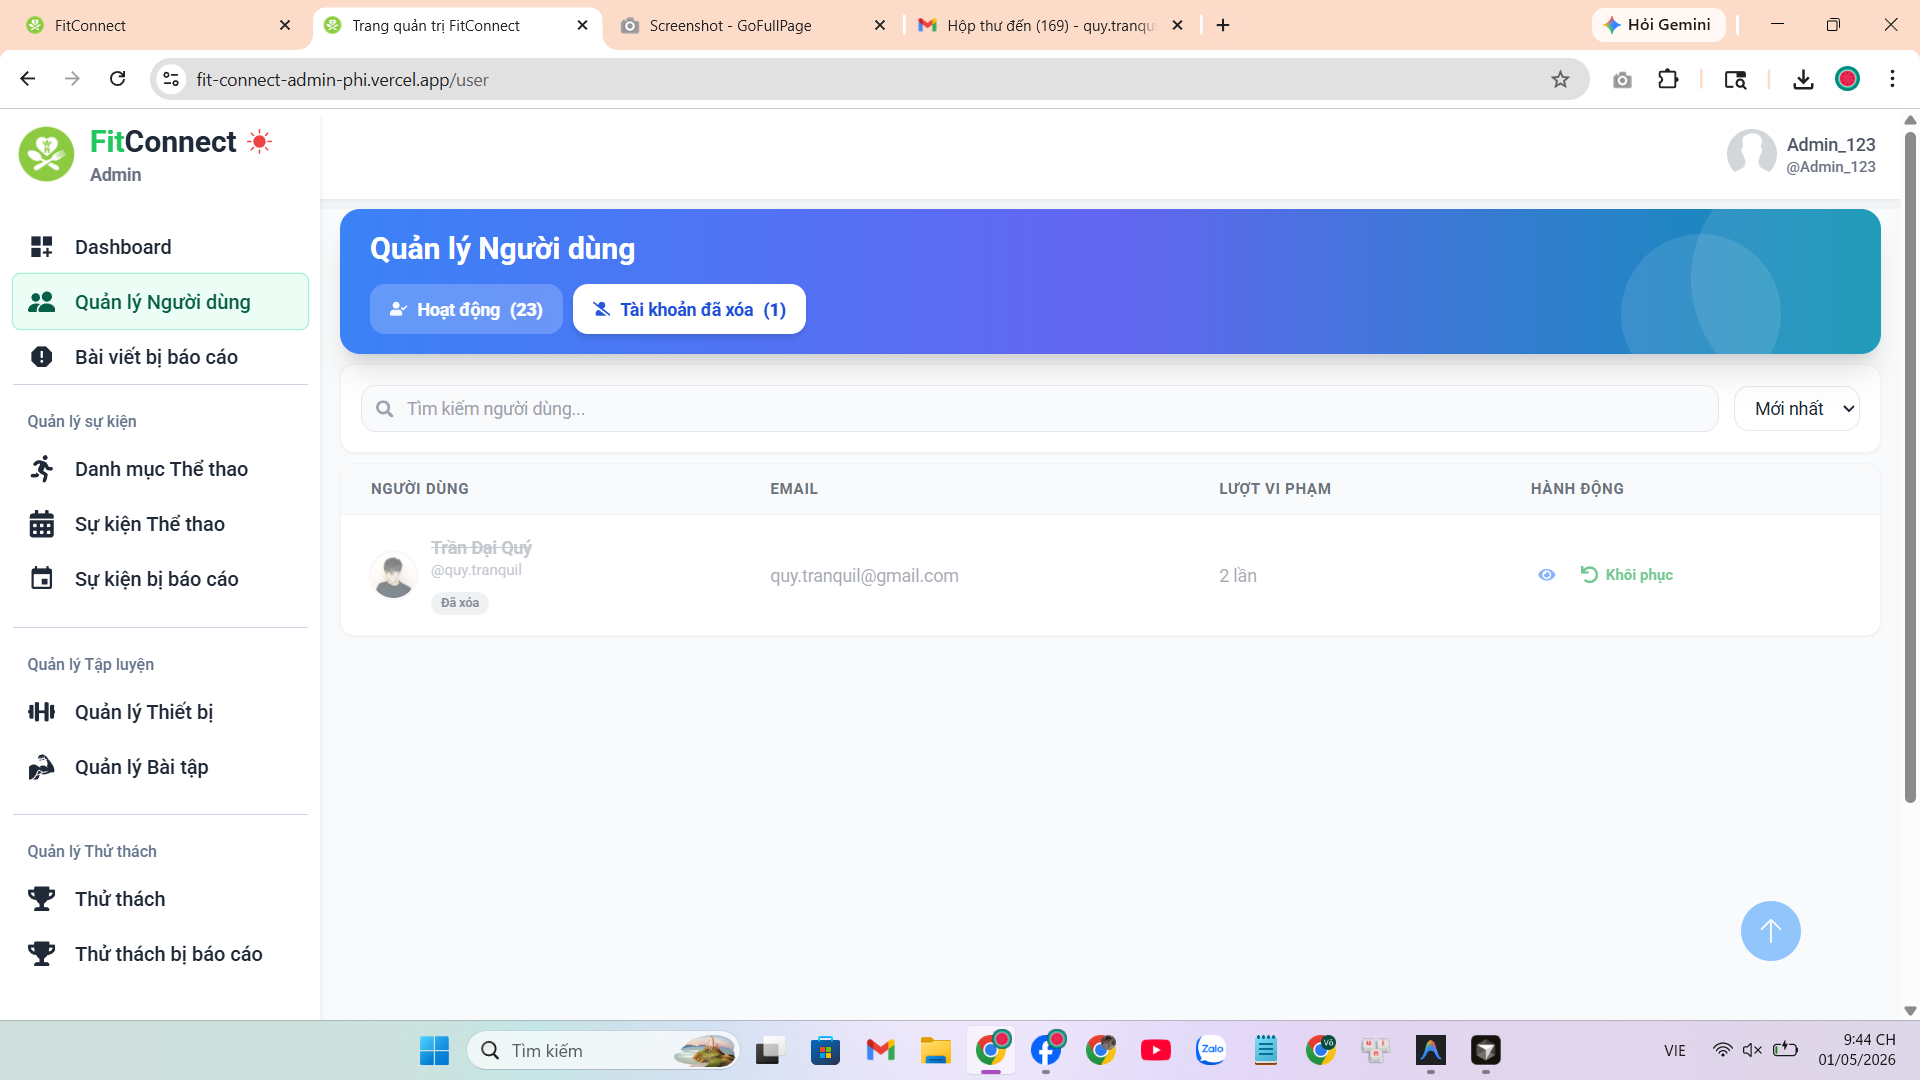
\includegraphics[width=\textwidth]{Images/IMG/nhom9/quanlynguoidung/nguoidungbixoa.png}
        \caption{Danh sách tài khoản đã bị vô hiệu hóa}
        \label{fig:impl_admin_user_deleted_list}
    \end{subfigure}
    \hfill
    \begin{subfigure}[b]{0.47\textwidth}
        \centering
        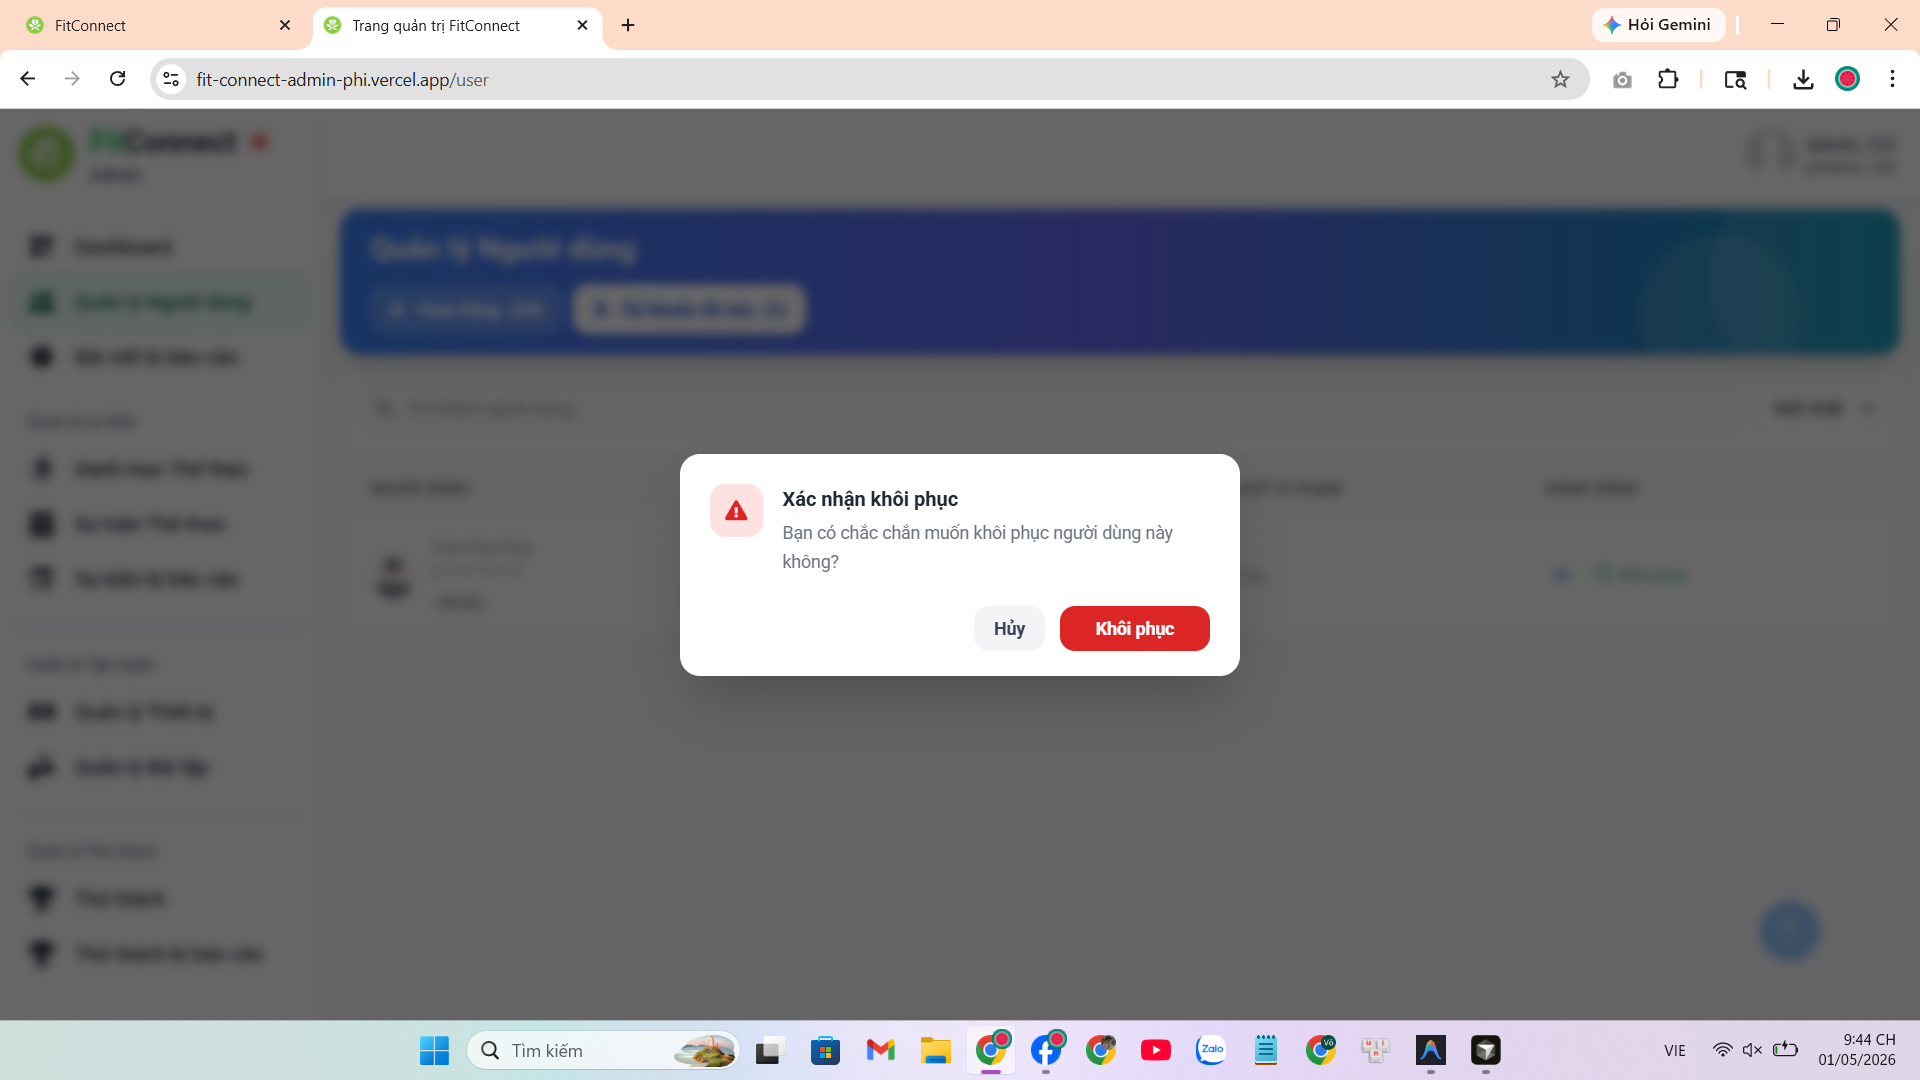
\includegraphics[width=\textwidth]{Images/IMG/nhom9/quanlynguoidung/modalkhoiphucnguoidungbixoa.png}
        \caption{Xác nhận khôi phục tài khoản người dùng}
        \label{fig:impl_admin_user_restore_confirm}
    \end{subfigure}
    \vspace{0.3em}
    \caption{Quản lý tài khoản bị vô hiệu hóa và quy trình khôi phục}
    \label{fig:impl_admin_user_ban_restore}
\end{figure}

\end{itemize}

\subsubsection{Luồng thao tác kiểm duyệt bài viết}
\begin{itemize}
    \item Quy trình kiểm duyệt bắt nguồn từ các báo cáo vi phạm của cộng đồng. Người dùng thao tác báo cáo nội dung không phù hợp trực tiếp trên bảng tin bài viết.

\begin{figure}[H]
    \centering
    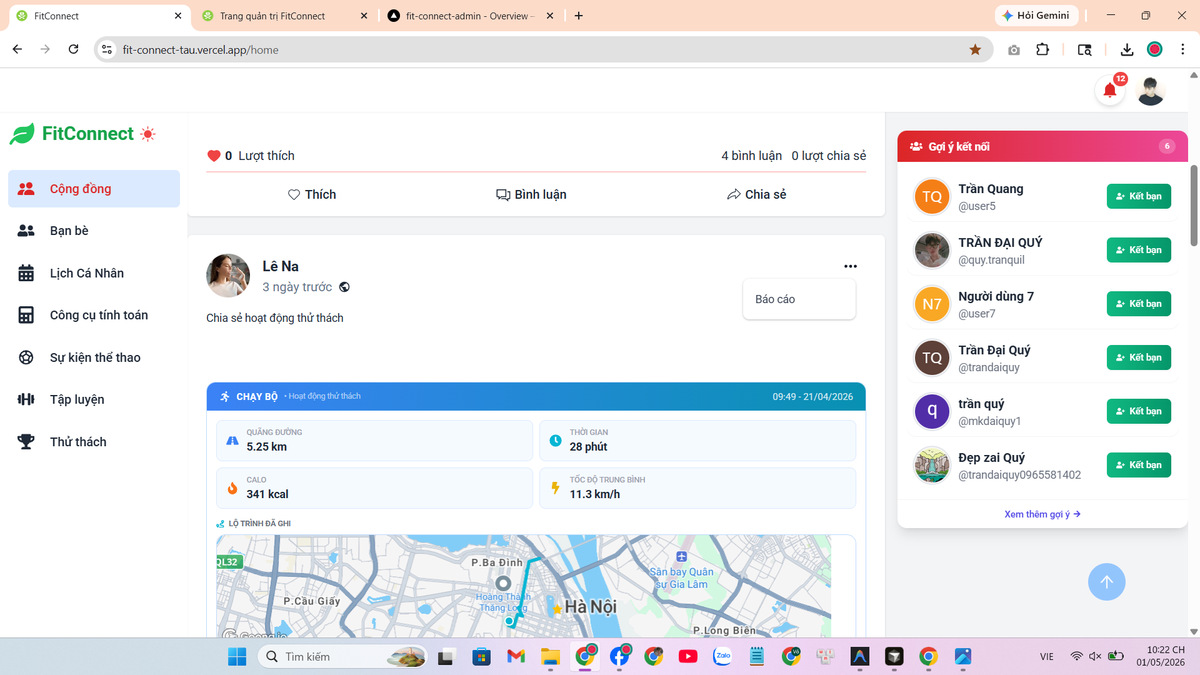
\includegraphics[width=0.60\textwidth]{Images/IMG/nhom9/quanlybaiviet/baocaobaiviet.png}
    \caption{Người dùng thực hiện báo cáo bài viết vi phạm trên trang Cộng đồng}
    \label{fig:impl_admin_post_report_action}
\end{figure}


    \item Tại trang kiểm duyệt, hệ thống tập hợp toàn bộ các báo cáo chờ xử lý. Quản trị viên có thể theo dõi danh sách các bài viết bị gắn cờ, kèm theo thông tin chi tiết về số lượng báo cáo và đánh giá mức độ nghiêm trọng.

\begin{figure}[H]
    \centering
    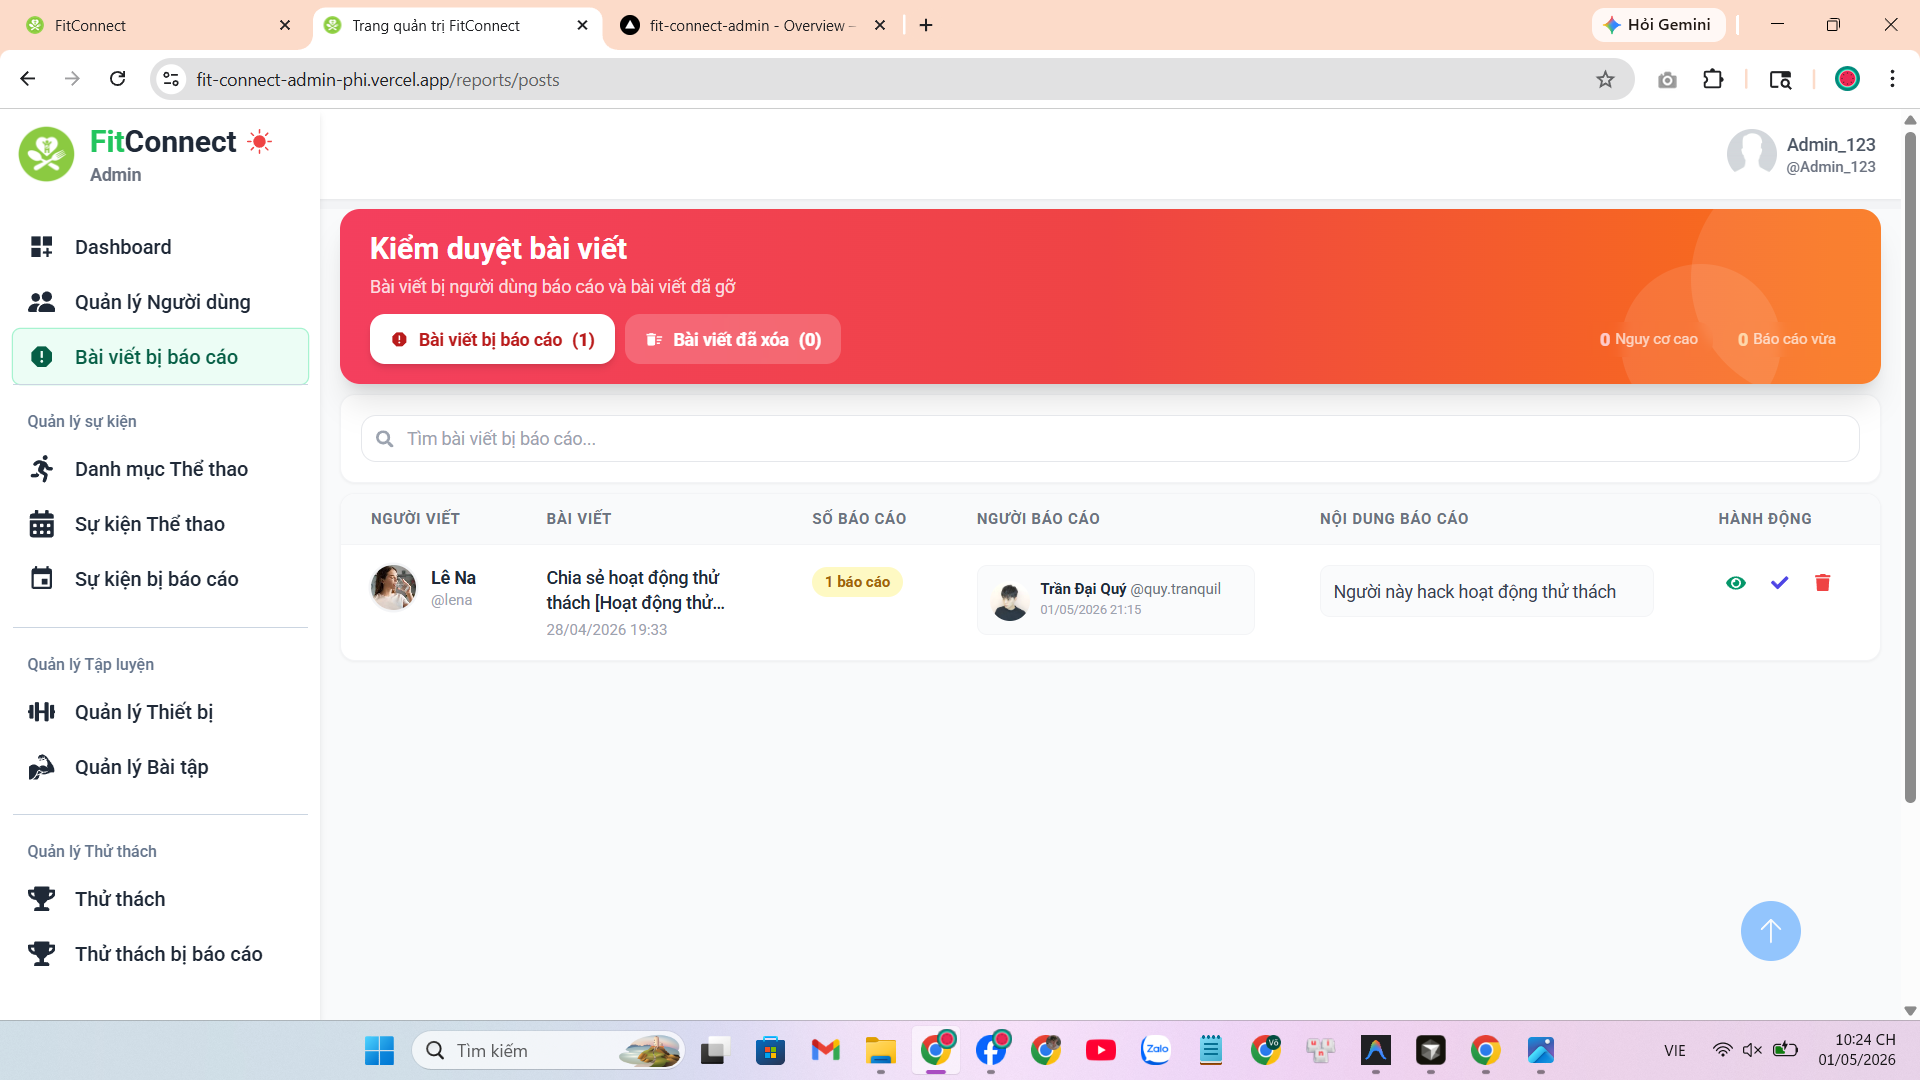
\includegraphics[width=0.60\textwidth]{Images/IMG/nhom9/quanlybaiviet/baivietbibaocao.png}
    \caption{Quản trị viên xem danh sách bài viết bị người dùng báo cáo}
    \label{fig:impl_admin_post_reported_list}
\end{figure}


    \item Để đảm bảo tính công bằng, hệ thống cung cấp giao diện hiển thị trọn vẹn nội dung bài viết gốc cùng danh sách lý do báo cáo, hỗ trợ Admin xem xét toàn diện trước khi đưa ra quyết định xử lý.

\begin{figure}[H]
    \centering
    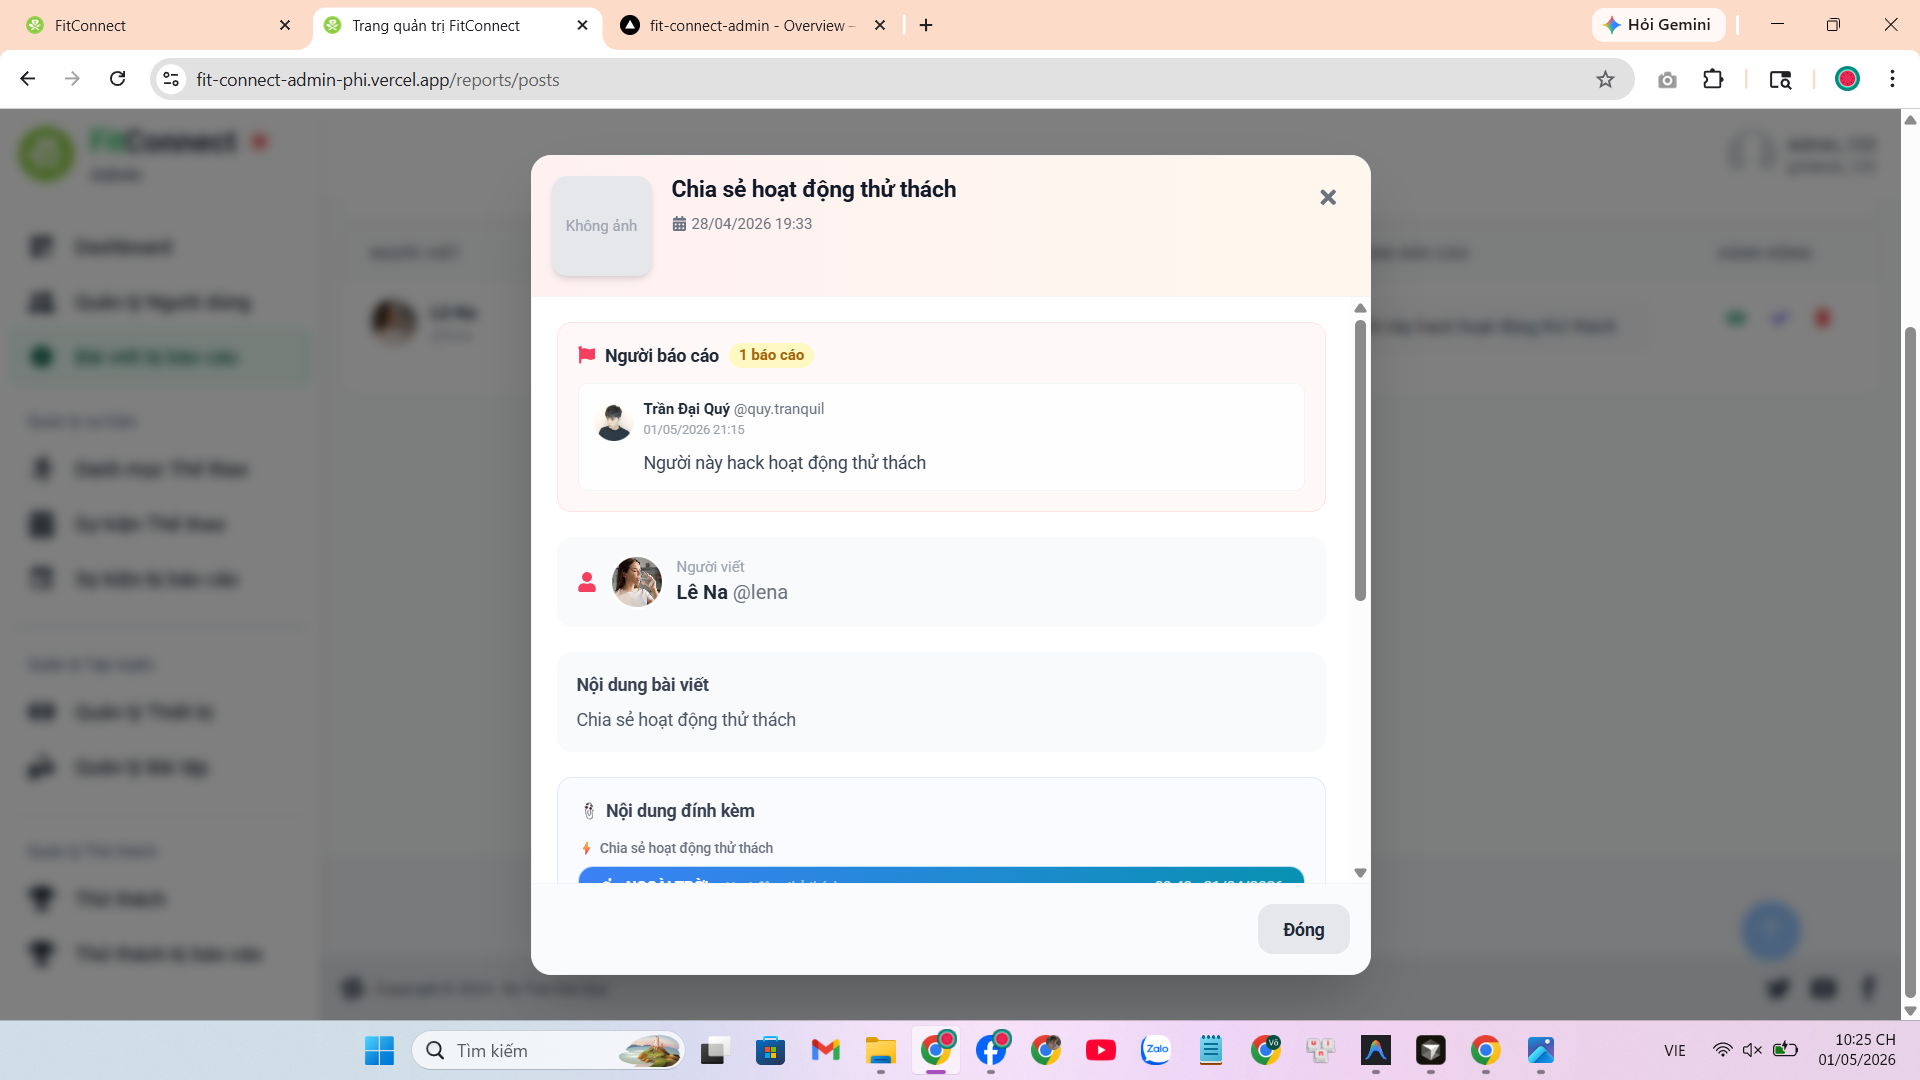
\includegraphics[width=0.60\textwidth]{Images/IMG/nhom9/quanlybaiviet/xemduocnoidungbaivietbibaocao.png}
    \caption{Quản trị viên xem chi tiết nội dung bài viết bị báo cáo kèm thông tin người báo cáo}
    \label{fig:impl_admin_post_report_detail}
\end{figure}


    \item Dựa trên phân tích, Admin \textbf{Gỡ bỏ} bài viết vi phạm (ẩn ngay khỏi bảng tin) hoặc \textbf{Giữ lại} nếu báo cáo không hợp lệ. Bài viết đã gỡ vào kho ``Đã xóa'' và có thể khôi phục trở lại bảng tin bất kỳ lúc nào.

\begin{figure}[H]
    \centering
    \begin{subfigure}[b]{0.47\textwidth}
        \centering
        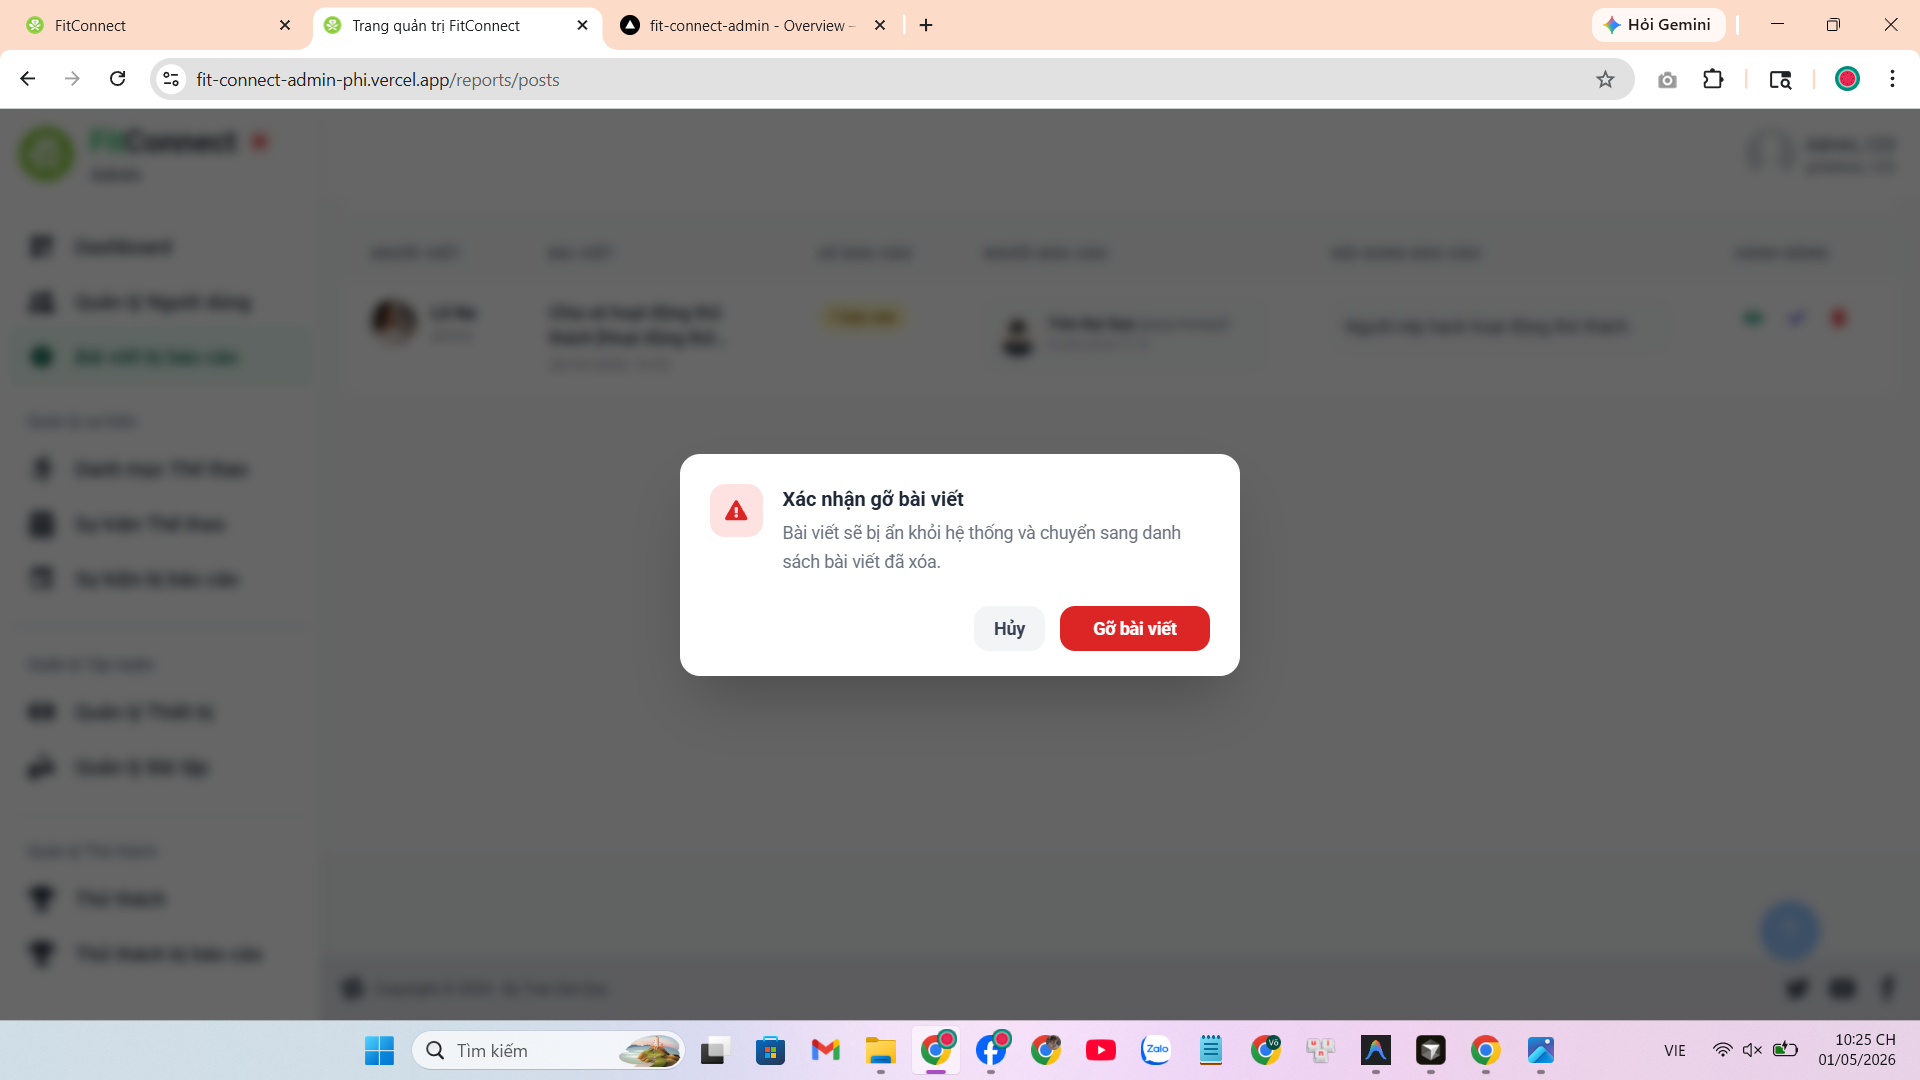
\includegraphics[width=\textwidth]{Images/IMG/nhom9/quanlybaiviet/xacnhanxoabaiviet.png}
        \caption{Xác nhận gỡ bài viết vi phạm}
        \label{fig:impl_admin_post_delete_confirm}
    \end{subfigure}
    \hfill
    \begin{subfigure}[b]{0.47\textwidth}
        \centering
        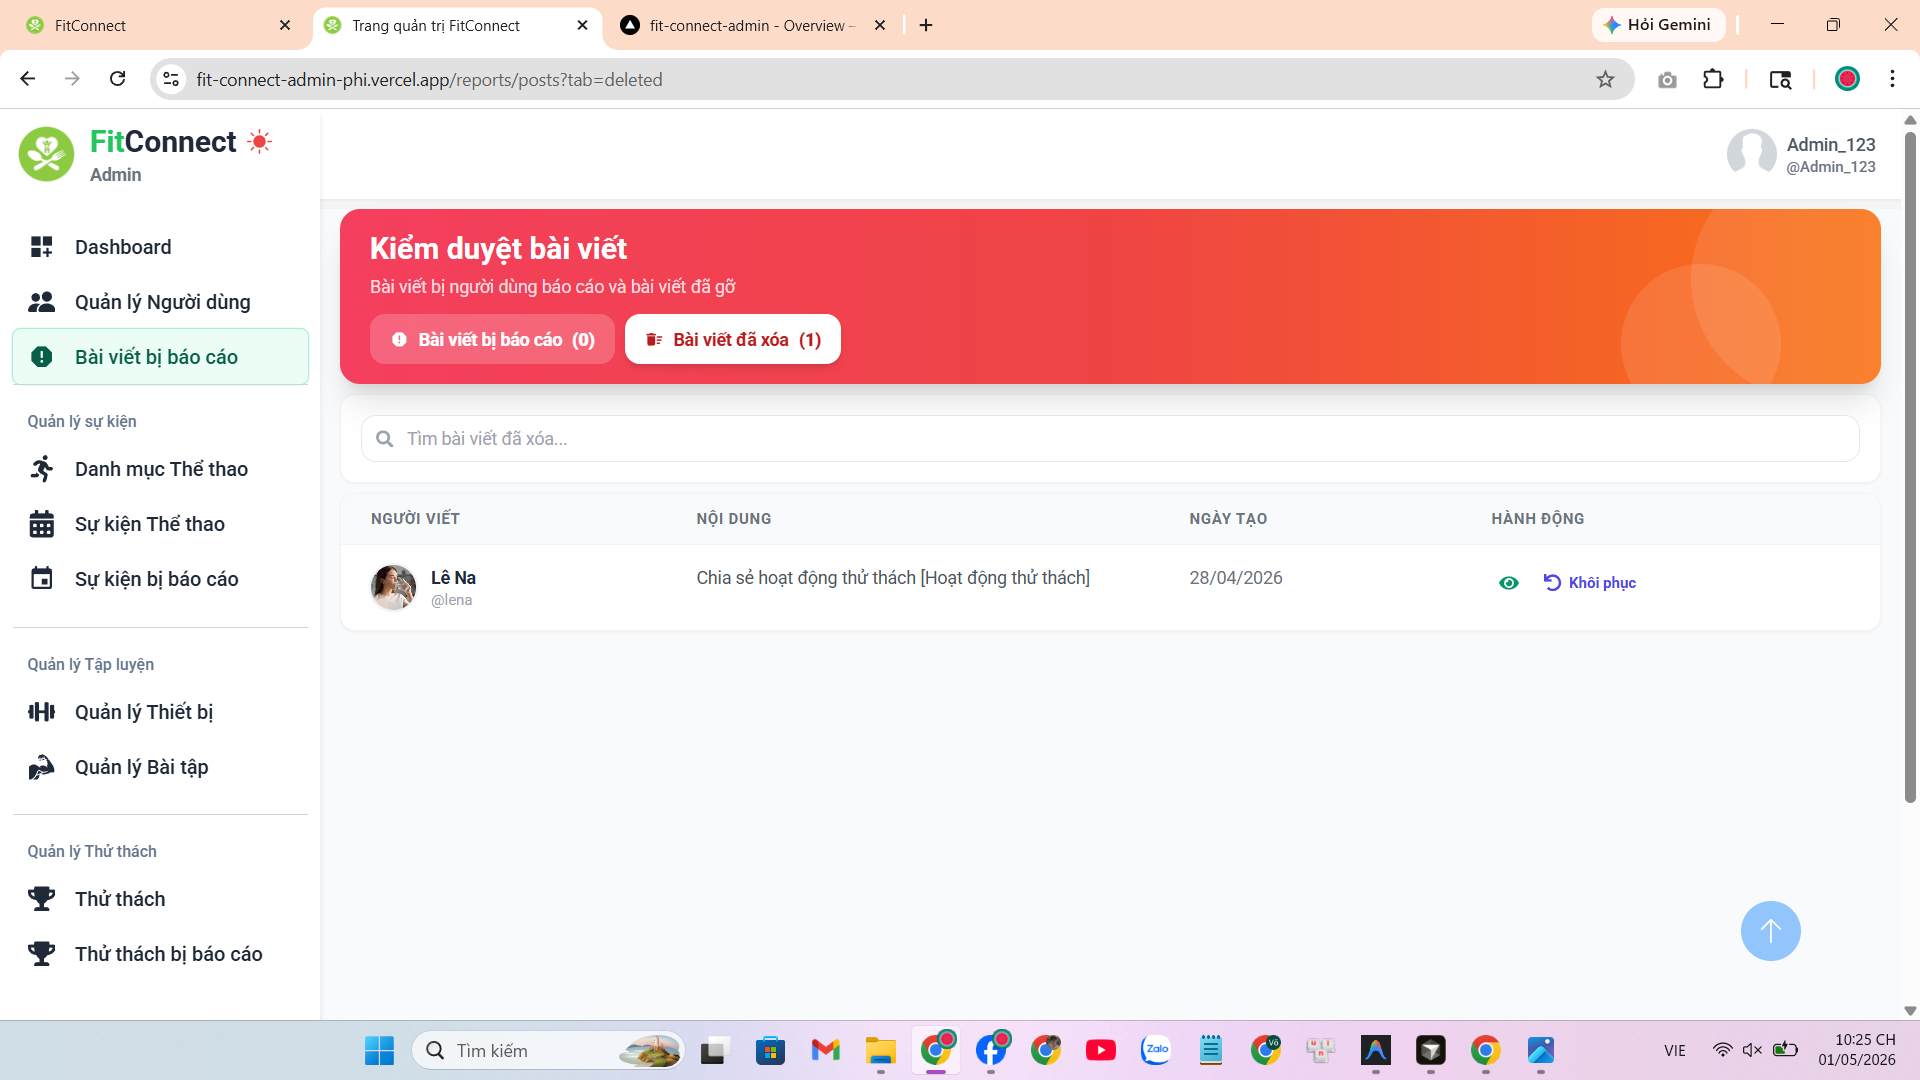
\includegraphics[width=\textwidth]{Images/IMG/nhom9/quanlybaiviet/danhsachbaivietbixoa.png}
        \caption{Danh sách bài viết đã gỡ và tùy chọn khôi phục}
        \label{fig:impl_admin_post_deleted_list}
    \end{subfigure}
    \vspace{0.3em}
    \caption{Xử lý bài viết vi phạm và quản lý kho lưu trữ bài viết đã gỡ}
    \label{fig:impl_admin_post_moderation}
\end{figure}

\end{itemize}

\subsubsection{Luồng thao tác quản lý danh mục thể thao}

\textbf{Cơ sở tính toán định mức Kcal:}

Để đảm bảo tính khoa học và nhất quán trên toàn nền tảng, hệ số tiêu thụ calo (Kcal) của từng môn thể thao được xây dựng dựa trên \textbf{Chỉ số chuyển hóa cơ bản (MET - Metabolic Equivalent of Task)}, tham chiếu trực tiếp từ cơ sở dữ liệu chuẩn quốc tế Compendium of Physical Activities \cite{CompendiumPhysicalActivities}. Hệ thống thực hiện chuẩn hóa số liệu bằng cách tính toán Kcal tiêu thụ trung bình dựa trên giả định cân nặng người dùng từ 65kg đến 70kg, nhằm tối ưu hóa hiệu suất xử lý hệ thống mà không yêu cầu cá nhân hóa theo từng người dùng.

Công thức tính toán gốc được áp dụng như sau:
\begin{itemize}
    \item Đối với hoạt động đo theo thời gian (phút): $\text{Kcal/phút} = \frac{\text{MET} \times 3.5 \times \text{Cân nặng (kg)}}{200}$
    \item Đối với hoạt động đo theo khoảng cách (km): $\text{Kcal/km} = \text{Kcal/phút} \times \text{Thời gian trung bình (phút) / km}$
\end{itemize}

Từ đó, hệ thống cấu hình tham số Kcal/Đơn vị và áp dụng vào hai luồng đo lường chính:
\begin{itemize}
    \item \textbf{Thể thao trong nhà (Tương tác qua Video Call):} $\text{Lượng Kcal} = \frac{\text{Thời gian hoạt động (giây)}}{60} \times \text{Kcal/phút}$. Trường hợp môn thể thao chưa được cập nhật hệ số, hệ thống sẽ sử dụng giá trị mặc định là $4\text{ Kcal/phút}$.
    \item \textbf{Thể thao ngoài trời (Theo dõi GPS):} $\text{Lượng Kcal} = \text{Khoảng cách (km)} \times \text{Kcal/km}$.
\end{itemize}

\textbf{Luồng thao tác quản trị trên hệ thống:}
\begin{itemize}
    \item Trang quản lý Danh mục Thể thao đóng vai trò là nơi cấu hình dữ liệu gốc cho toàn bộ các hoạt động thể chất trên nền tảng. Khi truy cập, Quản trị viên được cung cấp danh sách đầy đủ các môn thể thao đang được hỗ trợ, phân loại theo nhóm ``Ngoài trời'' và ``Trong nhà''. Mỗi danh mục hiển thị thông tin trực quan về tên môn, loại hình và định mức tiêu thụ calo (Kcal/Đơn vị) như đã trình bày ở trên.

\begin{figure}[H]
    \centering
    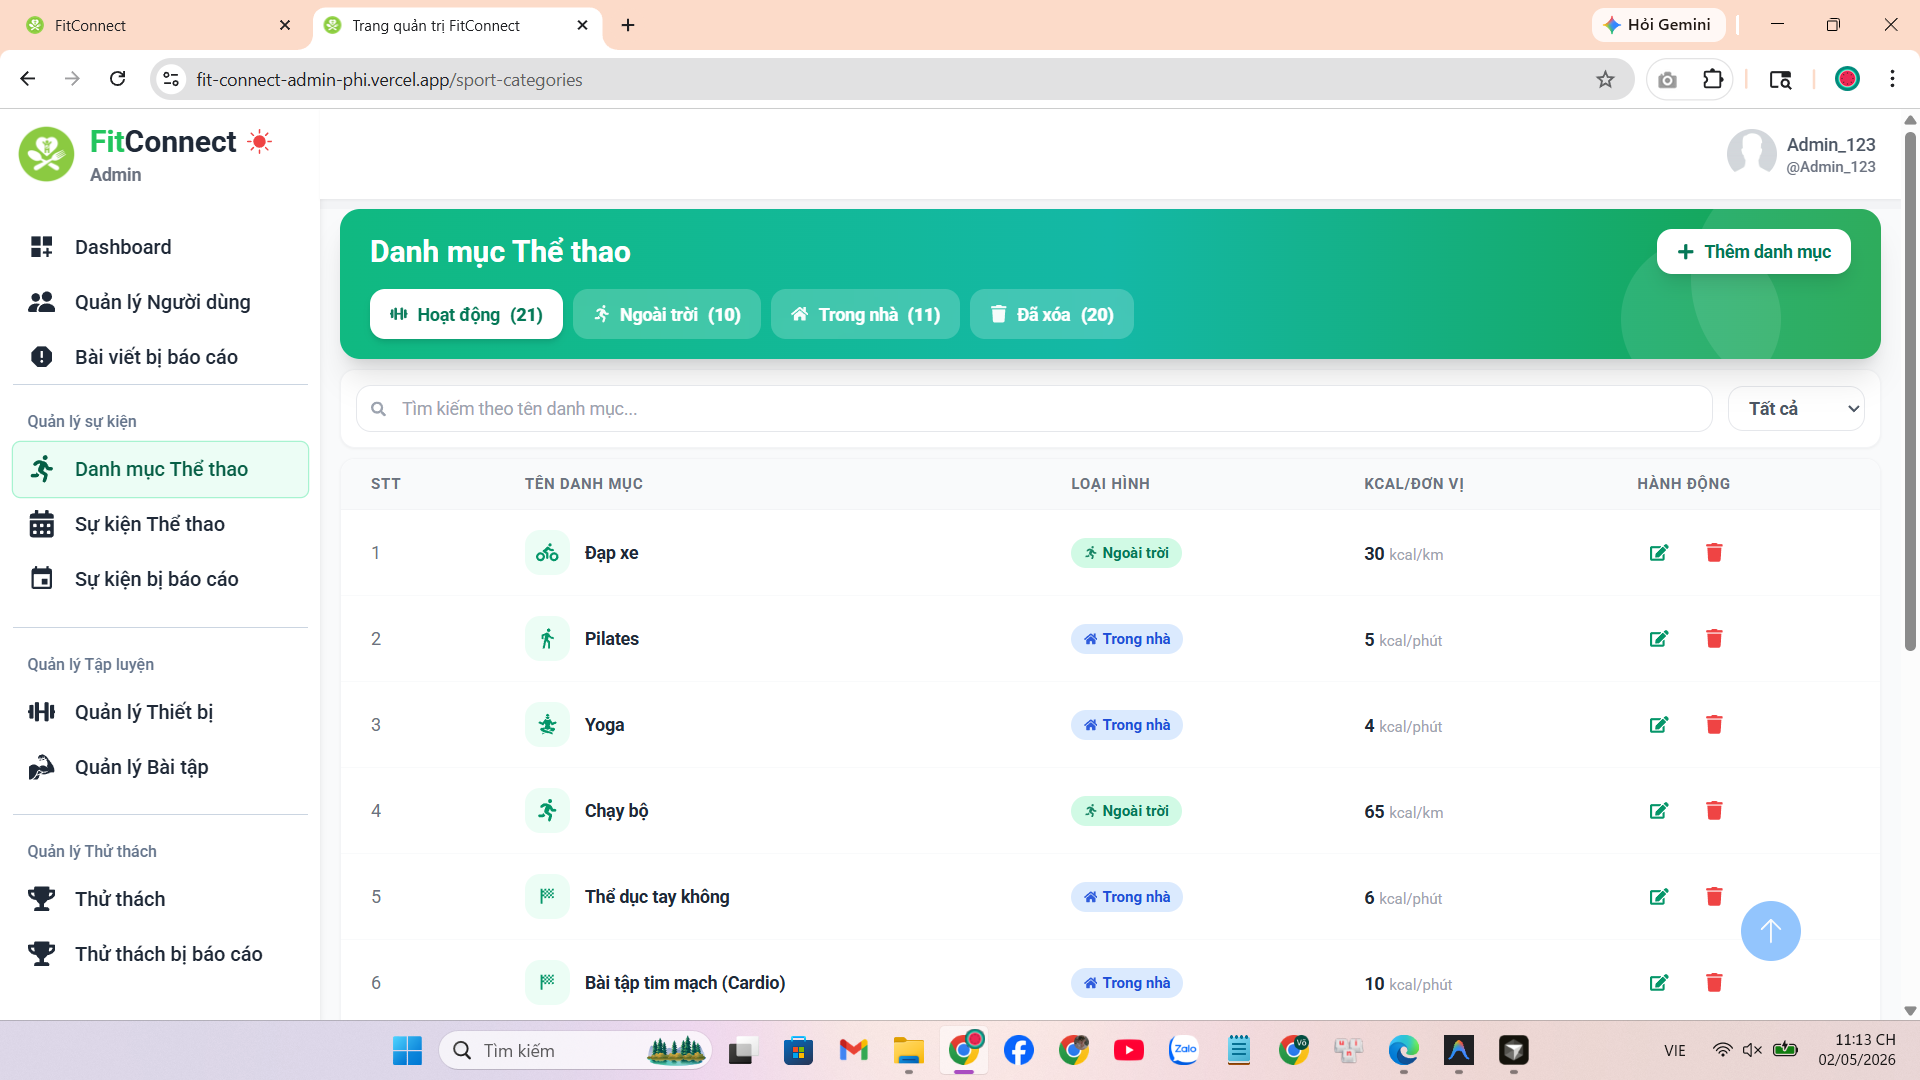
\includegraphics[width=0.60\textwidth]{Images/IMG/nhom9/danhmucthethao/danhsachdanhmucthethao.png}
    \caption{Quản trị viên xem danh sách các danh mục thể thao đang hoạt động}
    \label{fig:impl_admin_category_list}
\end{figure}


    \item Quản trị viên có thẩm quyền cập nhật các thông số của danh mục, đặc biệt là hệ số tiêu thụ Kcal. Khi thực hiện thay đổi trên hệ thống quản trị, giá trị này sẽ trở thành cơ sở tính toán mới cho toàn bộ các sự kiện và thử thách liên quan trên ứng dụng của người dùng.

\begin{figure}[H]
    \centering
    \begin{subfigure}[b]{0.47\textwidth}
        \centering
        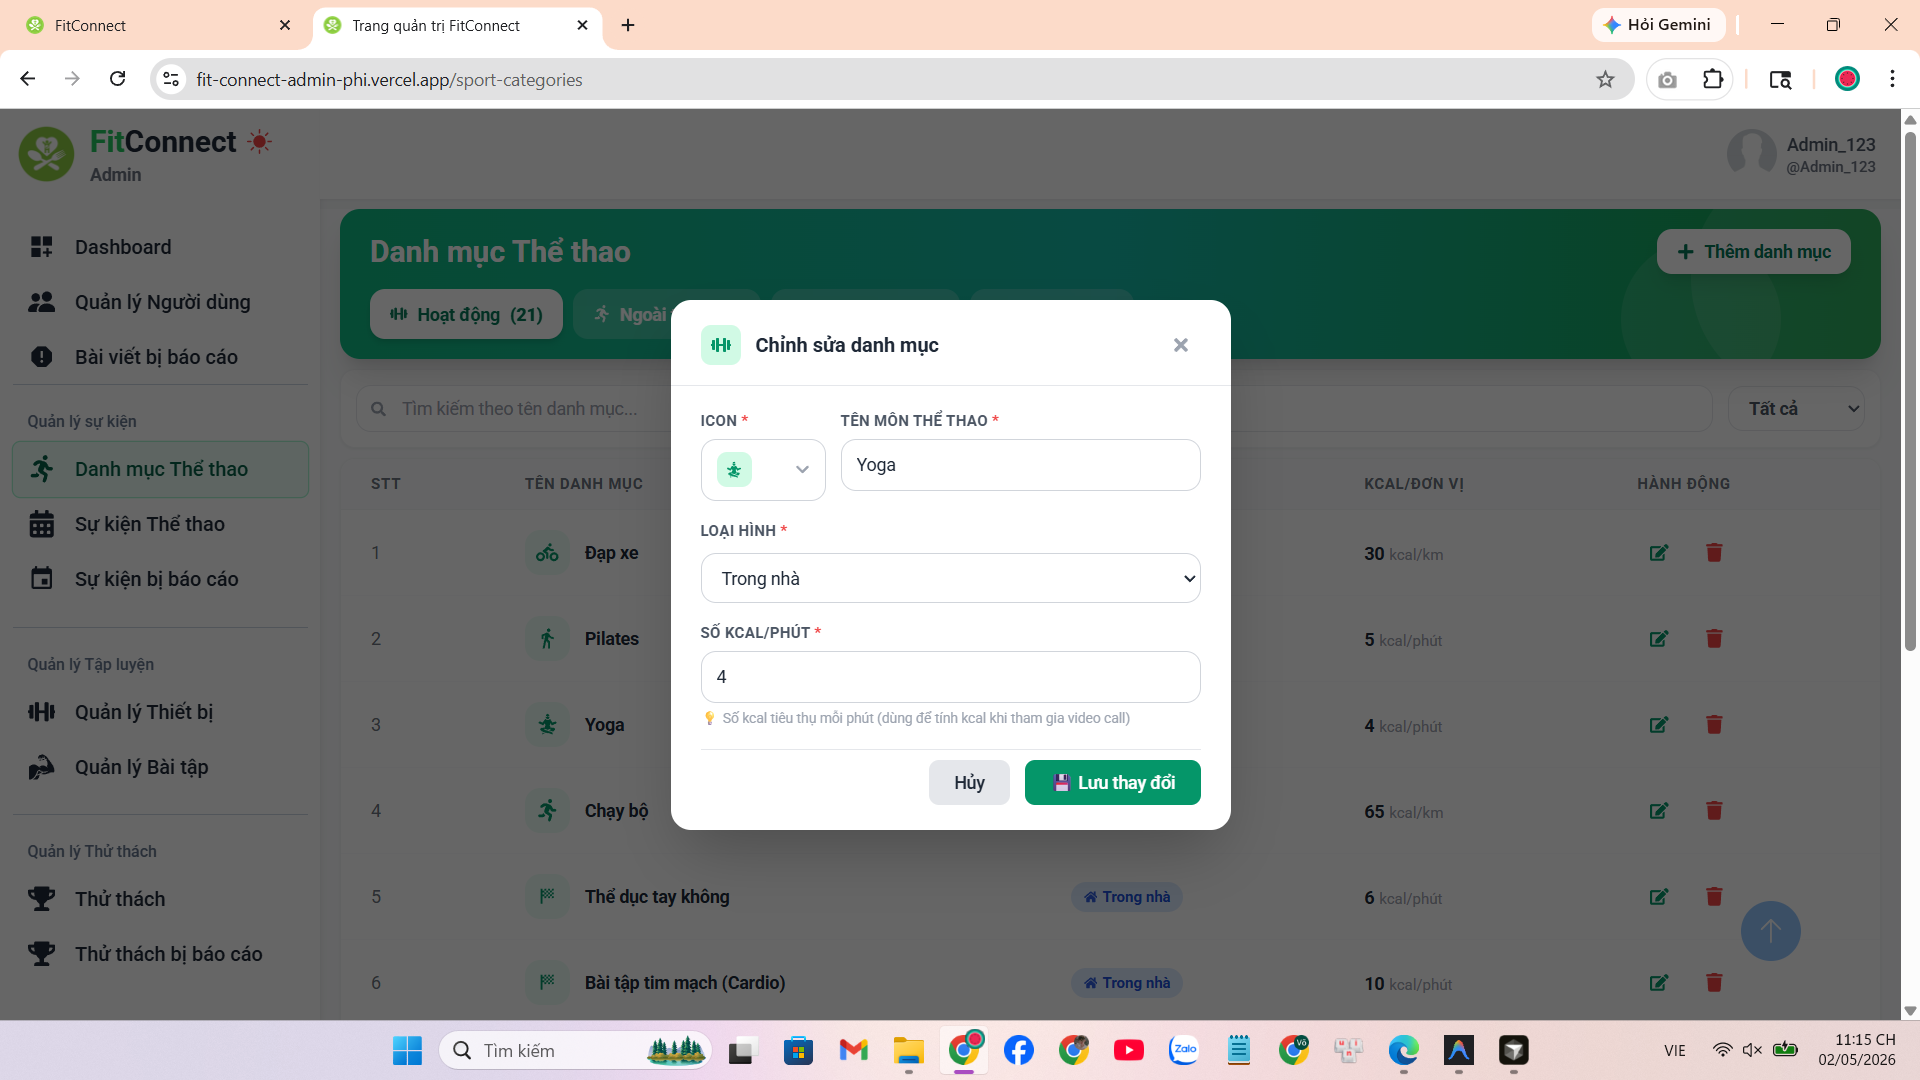
\includegraphics[width=\textwidth]{Images/IMG/nhom9/danhmucthethao/modalchinhsuadanhmuc.png}
        \caption{Hộp thoại chỉnh sửa thông tin danh mục}
        \label{fig:impl_admin_category_edit_modal}
    \end{subfigure}
    \hfill
    \begin{subfigure}[b]{0.47\textwidth}
        \centering
        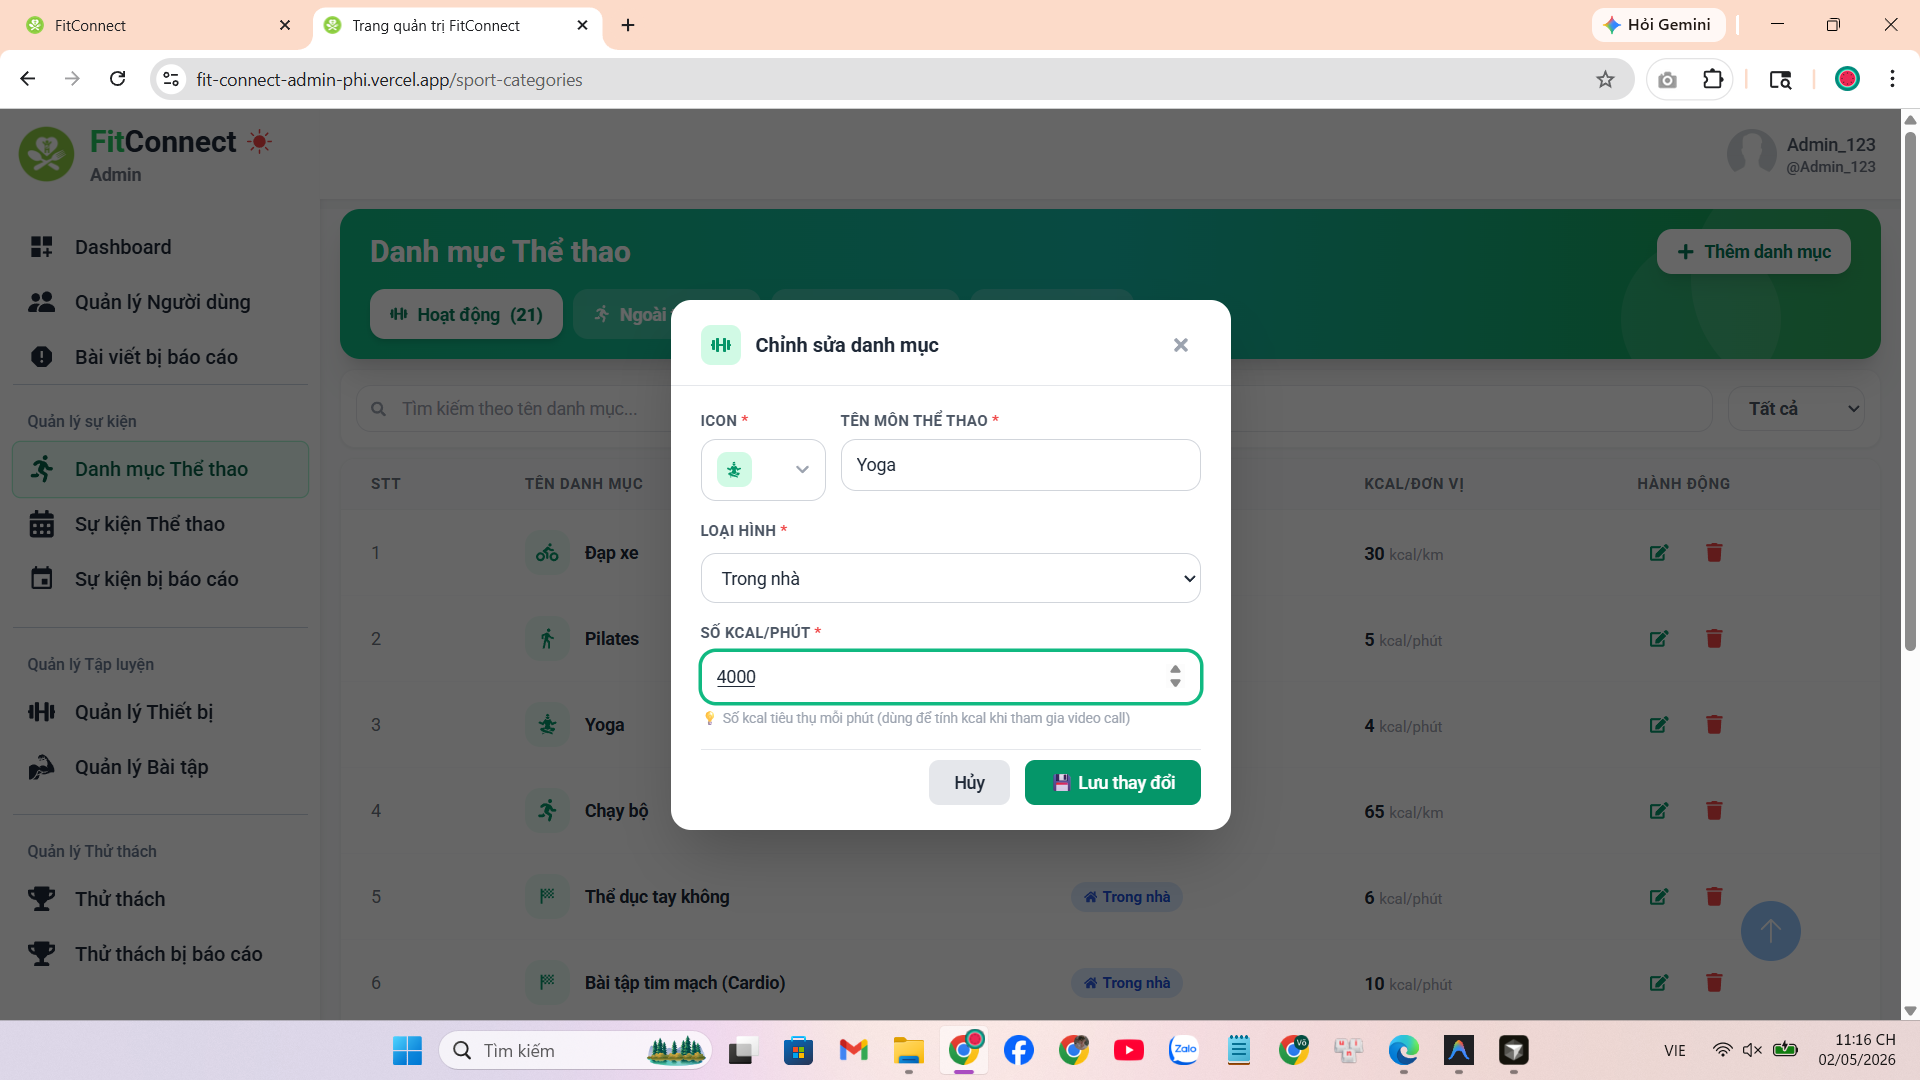
\includegraphics[width=\textwidth]{Images/IMG/nhom9/danhmucthethao/chinhsuathaydoisokcal.png}
        \caption{Thay đổi hệ số Kcal của môn thể thao}
        \label{fig:impl_admin_category_edit_kcal}
    \end{subfigure}
    \vspace{0.3em}
    \caption{Cập nhật thông số danh mục thể thao. Sau khi lưu, hệ số Kcal mới áp dụng ngay cho toàn bộ hoạt động liên quan.}
    \label{fig:impl_admin_category_edit}
\end{figure}


    \item Hệ thống hỗ trợ cơ chế vô hiệu hóa (xóa mềm) các môn thể thao không còn được hỗ trợ. Việc vô hiệu hóa sẽ ẩn danh mục khỏi danh sách lựa chọn tạo hoạt động mới của người dùng, nhưng không làm ảnh hưởng tới các dữ liệu lịch sử đã được ghi nhận trước đó.

\begin{figure}[H]
    \centering
    \begin{subfigure}[b]{0.47\textwidth}
        \centering
        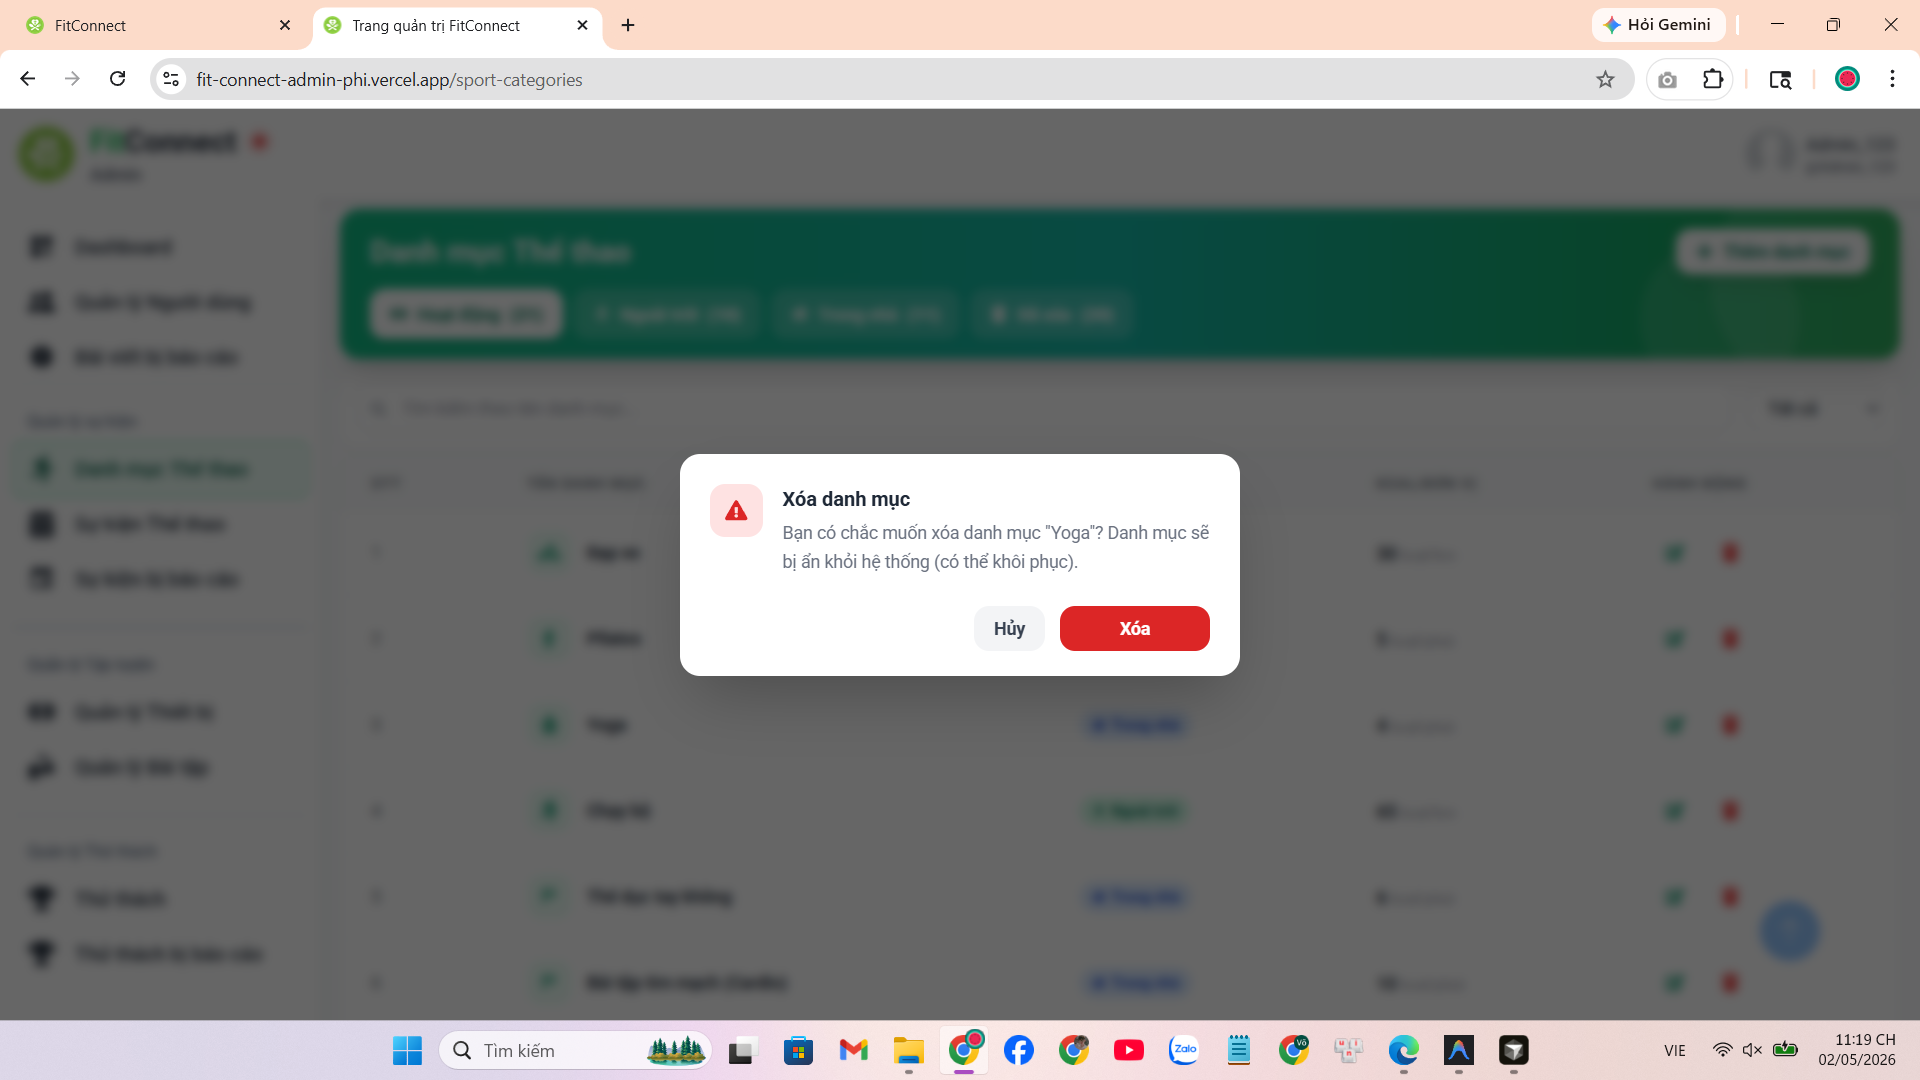
\includegraphics[width=\textwidth]{Images/IMG/nhom9/danhmucthethao/xoadanhmucyoga.png}
        \caption{Hệ thống hiển thị hộp thoại xác nhận vô hiệu hóa danh mục thể thao}
        \label{fig:impl_admin_category_delete}
    \end{subfigure}
    \hfill
    \begin{subfigure}[b]{0.47\textwidth}
        \centering
        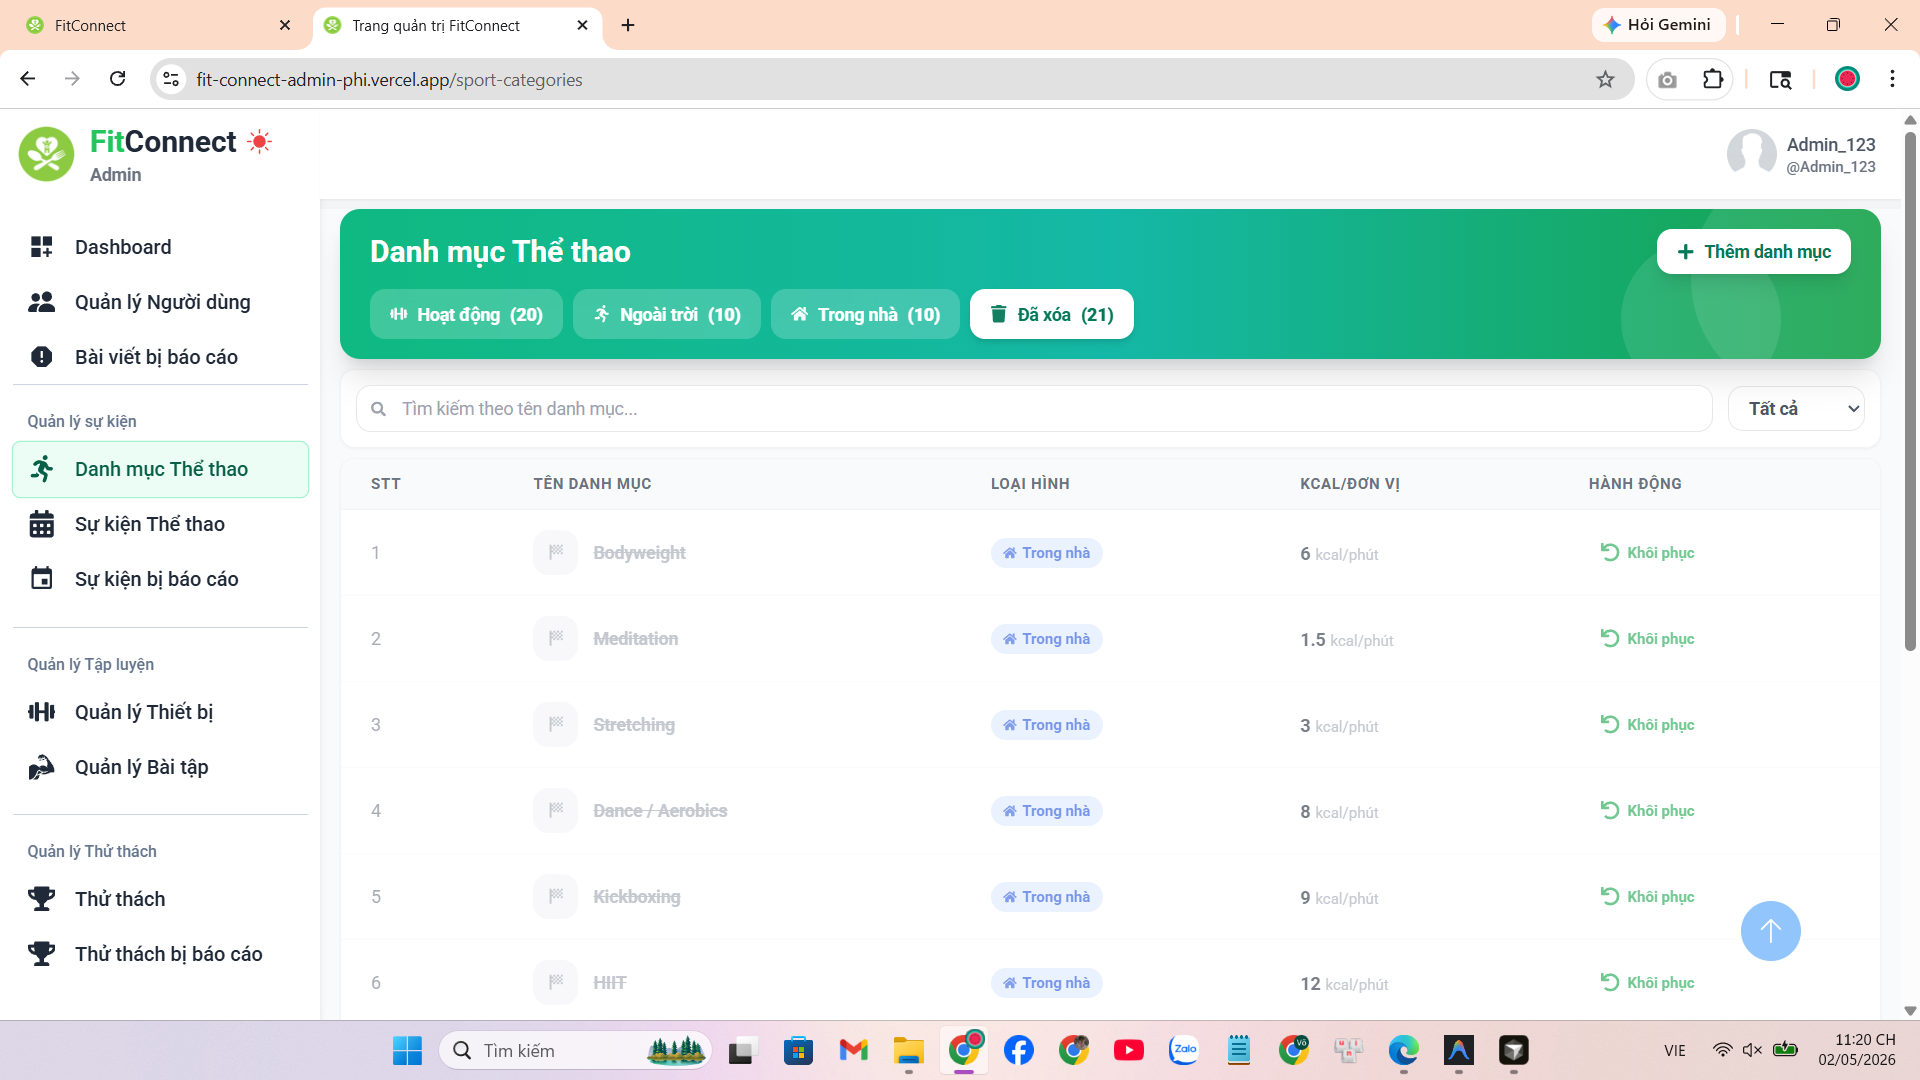
\includegraphics[width=\textwidth]{Images/IMG/nhom9/danhmucthethao/danhsachdanhmucdaxoa.png}
        \caption{Danh mục bị vô hiệu hóa được chuyển vào khu vực lưu trữ riêng biệt}
        \label{fig:impl_admin_category_deleted_list}
    \end{subfigure}
\end{figure}


    \item Các danh mục đã bị vô hiệu hóa có thể được khôi phục bất kỳ lúc nào. Sau khi khôi phục, danh mục hiển thị trở lại trong bảng cấu hình và sẵn sàng cho các hoạt động thể thao mới, đồng thời được tái tích hợp vào các sự kiện/thử thách liên quan.

\end{itemize}

\subsubsection{Luồng thao tác quản lý sự kiện thể thao}
\begin{itemize}
    \item Hệ thống cung cấp cho Quản trị viên bảng điều khiển tổng quan về tất cả các sự kiện thể thao đang diễn ra trên nền tảng. Danh sách hiển thị chi tiết các thông tin quan trọng như phân loại sự kiện (Trong nhà/Ngoài trời), thời gian tổ chức, địa điểm, tiến độ hoàn thành mục tiêu tập thể, và số lượng thành viên tham gia.

\begin{figure}[H]
    \centering
    
\includegraphics[width=0.60\textwidth]{Images/IMG/nhom9/quanlysukienthethao/danhsachsukien.png}
    \caption{Quản trị viên xem danh sách tổng hợp các sự kiện thể thao}
    \label{fig:impl_admin_event_list}
\end{figure}


    \item Để kiểm duyệt nội dung, Quản trị viên có thể xem phân tích chi tiết của từng sự kiện thông qua hộp thoại hiển thị nhanh. Chức năng này giúp Admin đánh giá tính hợp lệ của mục tiêu đề ra (ví dụ: quãng đường cần đạt) cũng như nội dung mô tả của người tổ chức.

\begin{figure}[H]
    \centering
    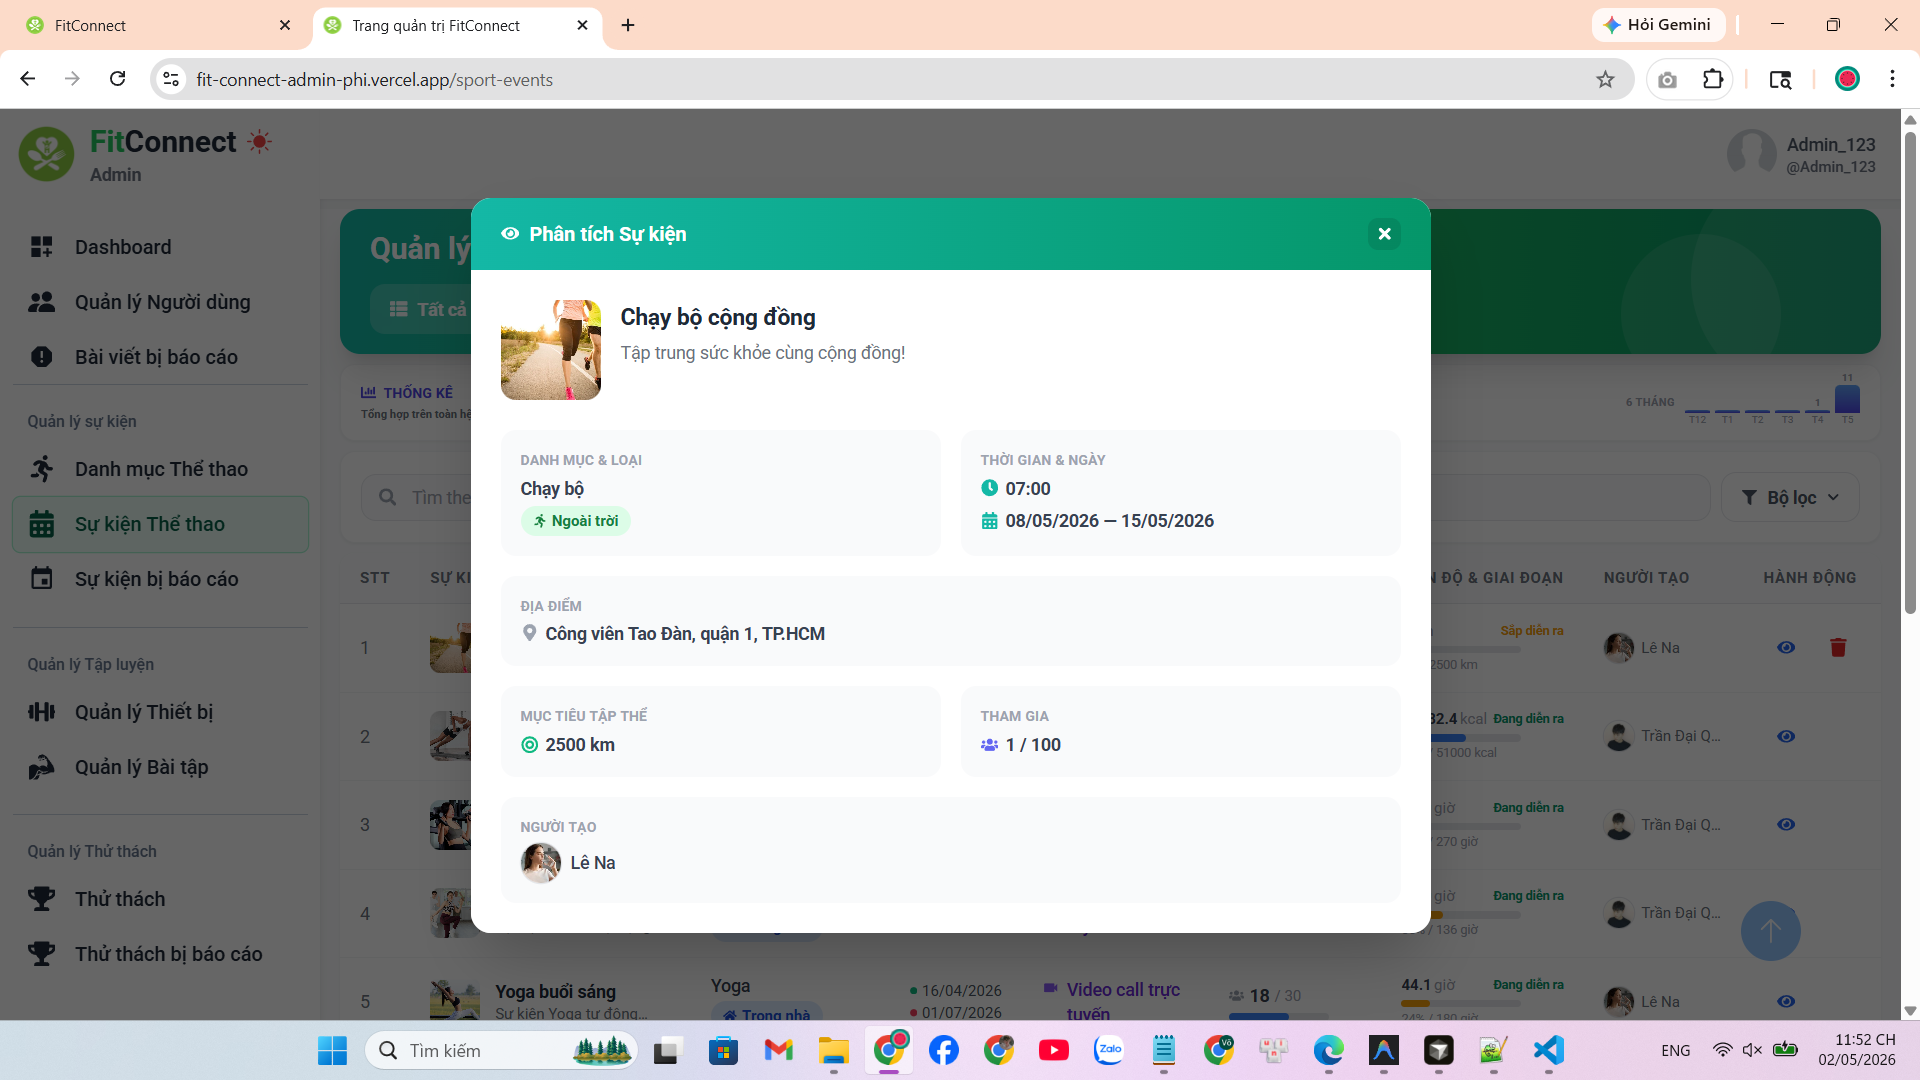
\includegraphics[width=0.60\textwidth]{Images/IMG/nhom9/quanlysukienthethao/xemthongtinsukien.png}
    \caption{Hệ thống hiển thị hộp thoại phân tích chi tiết thông tin sự kiện}
    \label{fig:impl_admin_event_detail}
\end{figure}


    \item Trong trường hợp phát hiện sự kiện vi phạm tiêu chuẩn cộng đồng hoặc chứa thông tin sai lệch, Quản trị viên có quyền can thiệp vô hiệu hóa sự kiện. Hệ thống sẽ yêu cầu xác nhận để tránh các thao tác sai lầm do vô ý.

\begin{figure}[H]
    \centering
    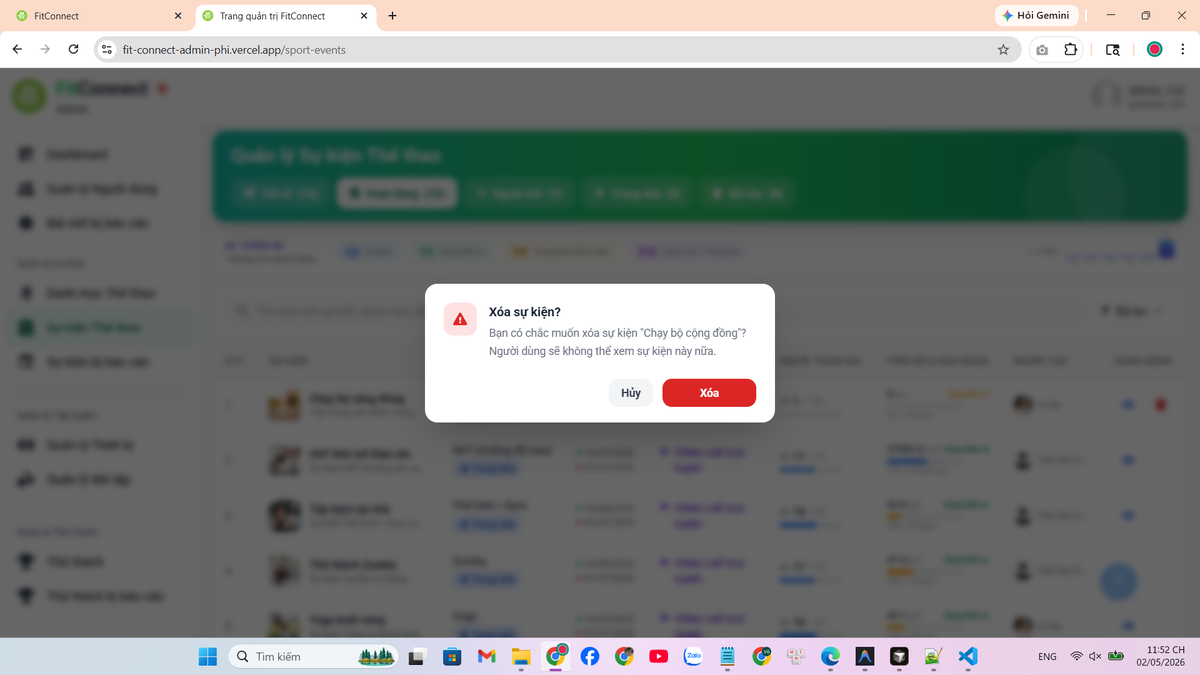
\includegraphics[width=0.60\textwidth]{Images/IMG/nhom9/quanlysukienthethao/modalxoasukien.png}
    \caption{Hệ thống hiển thị hộp thoại xác nhận vô hiệu hóa sự kiện}
    \label{fig:impl_admin_event_delete_confirm}
\end{figure}


    \item Khi sự kiện bị vô hiệu hóa, thay vì bị xóa hoàn toàn khỏi hệ thống, sự kiện sẽ được chuyển sang chế độ chỉ đọc (Read-only). Tại trạng thái này, người dùng vẫn có thể xem được các thông tin cơ bản và lịch sử của sự kiện nhưng mọi tính năng tương tác như tham gia, rời nhóm hay cập nhật tiến độ đều bị vô hiệu hóa để đảm bảo tính minh bạch của dữ liệu.
% \begin{figure}[H]
%     \centering
%     
\includegraphics[width=0.8\textwidth]{Images/IMG/nhom3/sukiensaukhixoa.png}
%     \vspace{1em}
%     \caption{Giao diện sự kiện chuyển sang chế độ chỉ đọc sau khi bị Quản trị viên vô hiệu hóa}
%     \label{fig:impl_admin_event_readonly_view}
% \end{figure}

    \item Nhằm quản lý rủi ro và hỗ trợ xử lý khiếu nại, các sự kiện bị vô hiệu hóa không bị xóa vĩnh viễn mà được lưu trữ trong danh sách ``Đã xóa''. Tại đây, Quản trị viên có thể xem lại lịch sử và thực hiện thao tác khôi phục nếu xác định sự kiện hoàn toàn hợp lệ.

\begin{figure}[H]
    \centering
    \begin{subfigure}[b]{0.47\textwidth}
        \centering
        
\includegraphics[width=\textwidth]{Images/IMG/nhom9/quanlysukienthethao/danhsachsukiendaxoa.png}
        \caption{Các sự kiện bị vô hiệu hóa được hệ thống lưu trữ tại danh mục riêng}
        \label{fig:impl_admin_event_deleted_list}
    \end{subfigure}
    \hfill
    \begin{subfigure}[b]{0.47\textwidth}
        \centering
        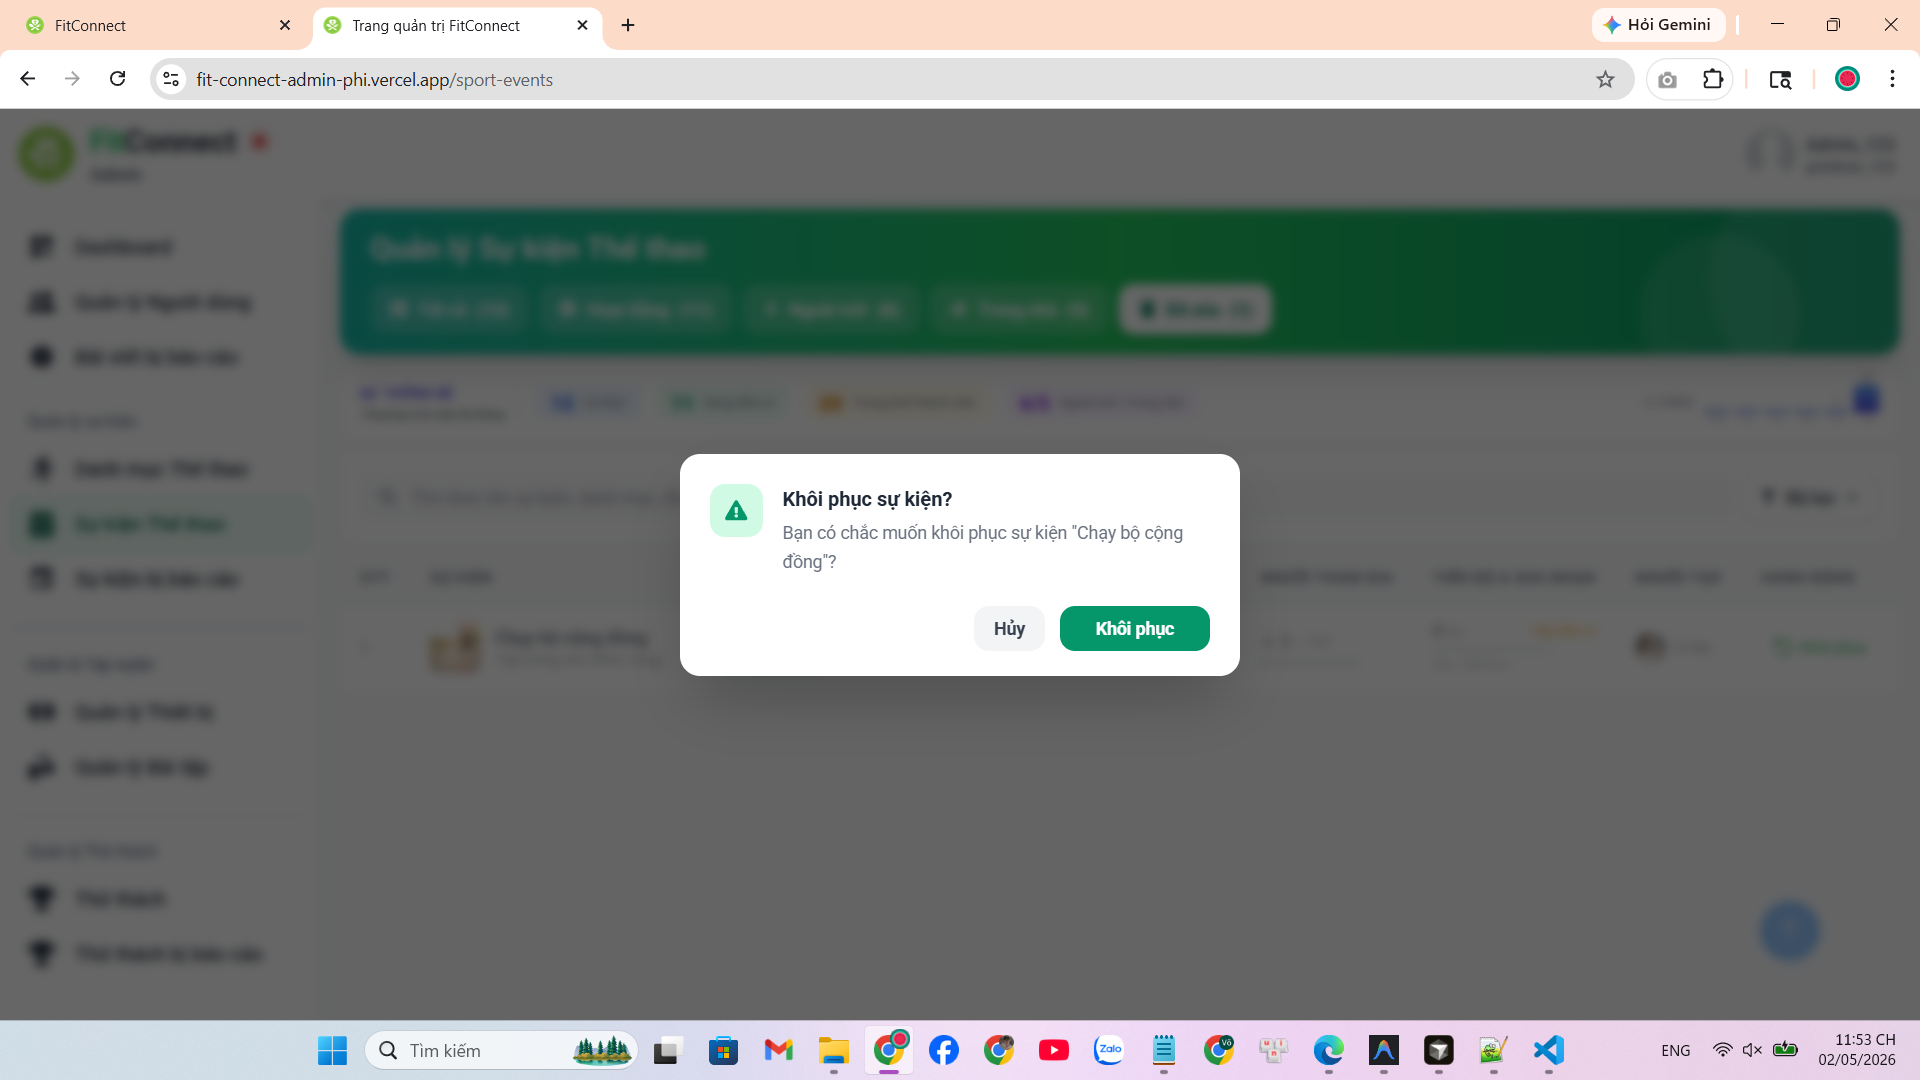
\includegraphics[width=\textwidth]{Images/IMG/nhom9/quanlysukienthethao/khoiphucsukien.png}
        \caption{Hệ thống hiển thị hộp thoại xác nhận khôi phục sự kiện}
        \label{fig:impl_admin_event_restore_confirm}
    \end{subfigure}
\end{figure}


    \item Sau khi khôi phục, sự kiện xuất hiện trở lại trên danh sách hoạt động chung. Mọi liên kết, tiến độ và danh sách người tham gia được bảo toàn nguyên vẹn, cho phép người dùng tiếp tục tương tác bình thường.

\end{itemize}

\subsubsection{Luồng thao tác kiểm duyệt sự kiện thể thao}
\begin{itemize}
    \item Tương tự cơ chế kiểm duyệt bài viết cộng đồng, hệ thống cung cấp tính năng báo cáo dành cho người dùng khi phát hiện các sự kiện thể thao có dấu hiệu gian lận, nội dung phản cảm hoặc vi phạm tiêu chuẩn nền tảng. Người dùng có thể cung cấp lý do chi tiết để hỗ trợ quá trình xử lý của Quản trị viên.

\begin{figure}[H]
    \centering
    \begin{subfigure}[b]{0.47\textwidth}
        \centering
        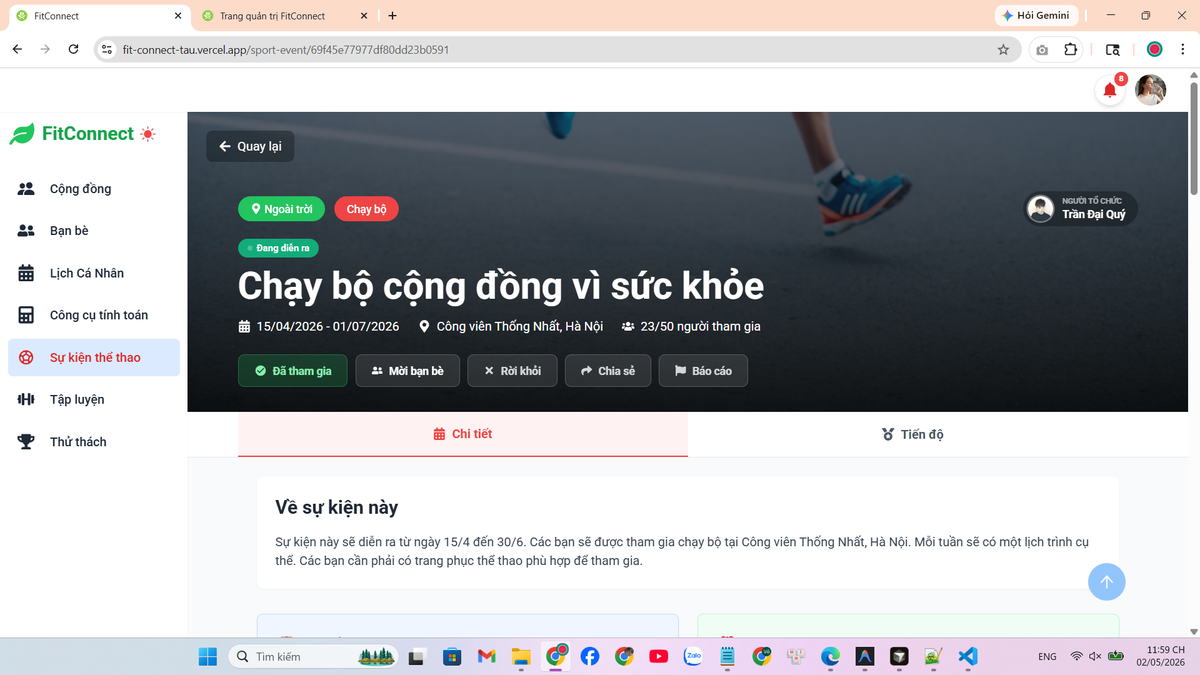
\includegraphics[width=\textwidth]{Images/IMG/nhom9/kiemduyetsukienthethao/sukienbenUser.png}
        \caption{Người dùng tương tác với sự kiện trên ứng dụng}
        \label{fig:impl_admin_event_mod_user_view}
    \end{subfigure}
    \hfill
    \begin{subfigure}[b]{0.47\textwidth}
        \centering
        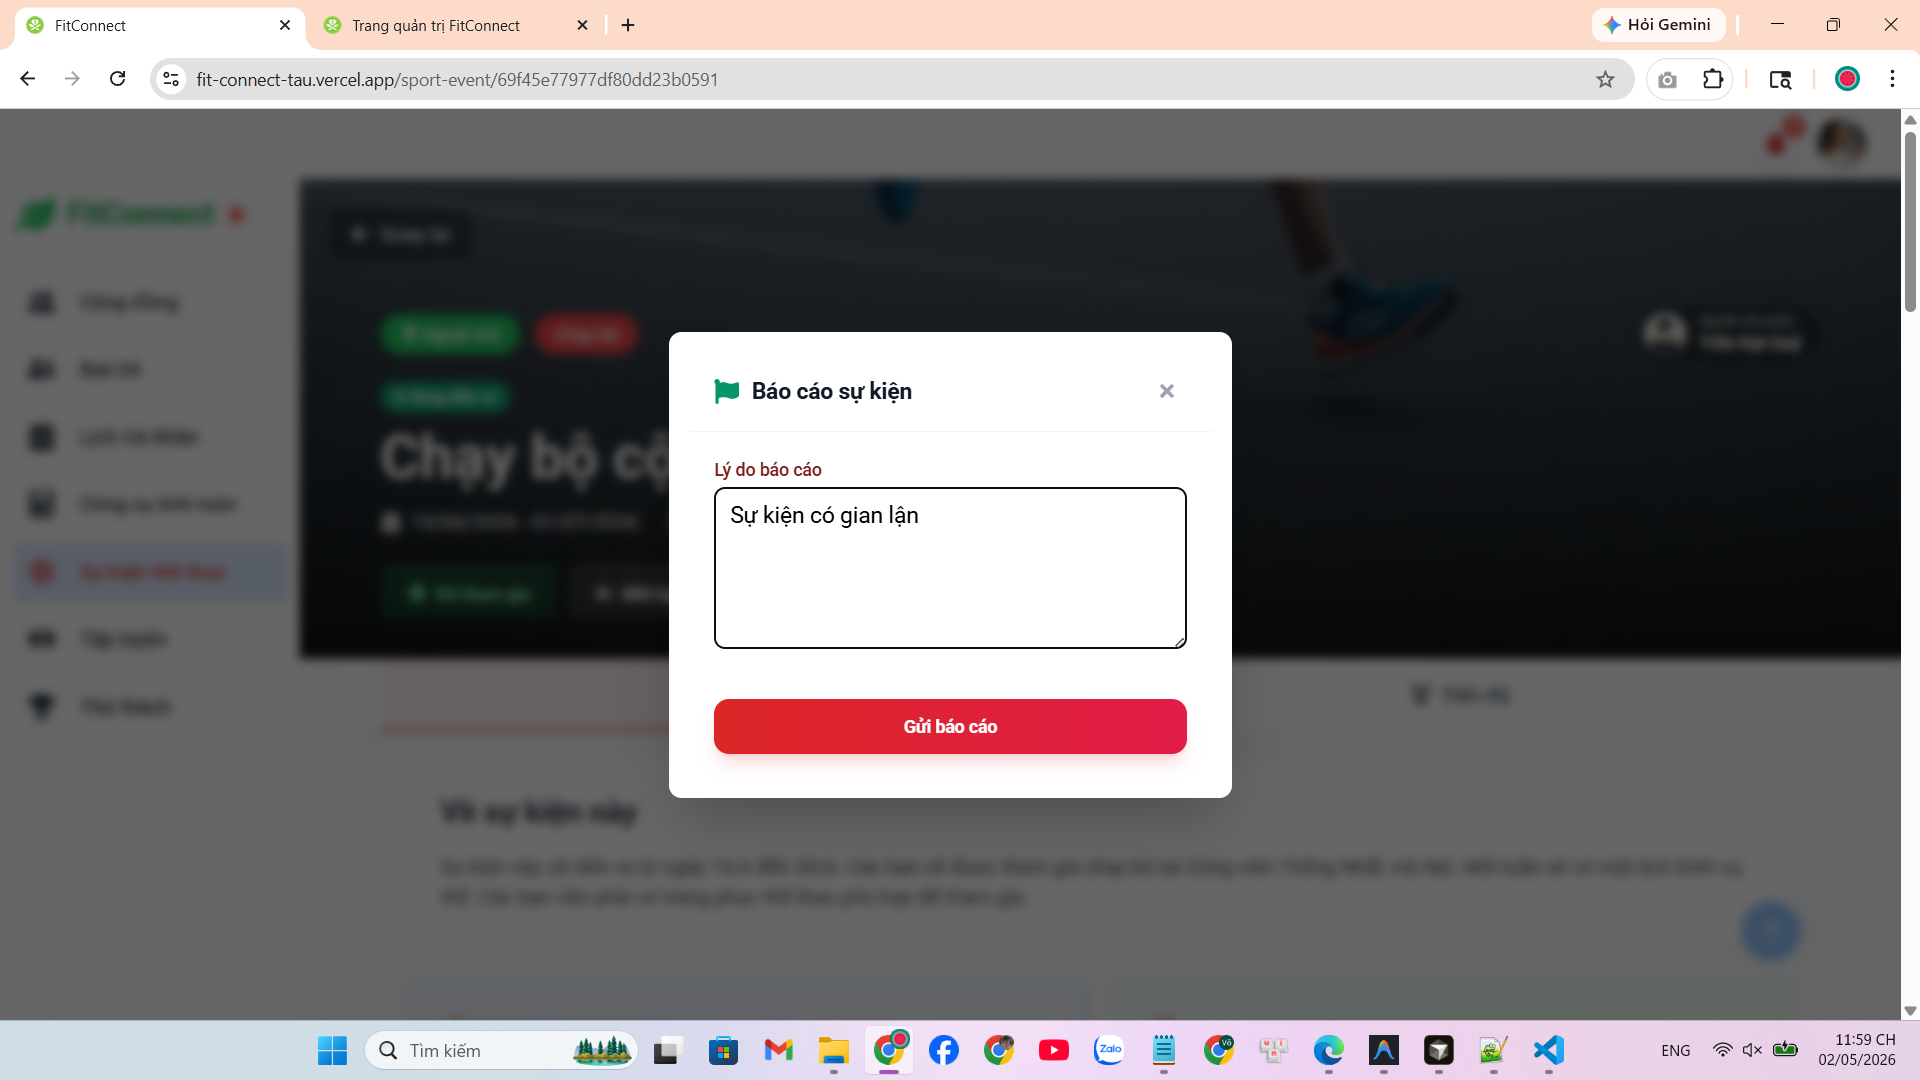
\includegraphics[width=\textwidth]{Images/IMG/nhom9/kiemduyetsukienthethao/Nguoidungbaocaosukien.png}
        \caption{Người dùng gửi báo cáo vi phạm đối với một sự kiện thể thao}
        \label{fig:impl_admin_event_mod_user_report}
    \end{subfigure}
\end{figure}


    \item Tại trang quản trị, các sự kiện bị báo cáo được tổng hợp thành một danh sách chờ xử lý. Giao diện cung cấp đầy đủ thông tin về người tạo, tên sự kiện, tổng số lượt báo cáo, thông tin người báo cáo và nội dung vi phạm bị cáo buộc.

\begin{figure}[H]
    \centering
    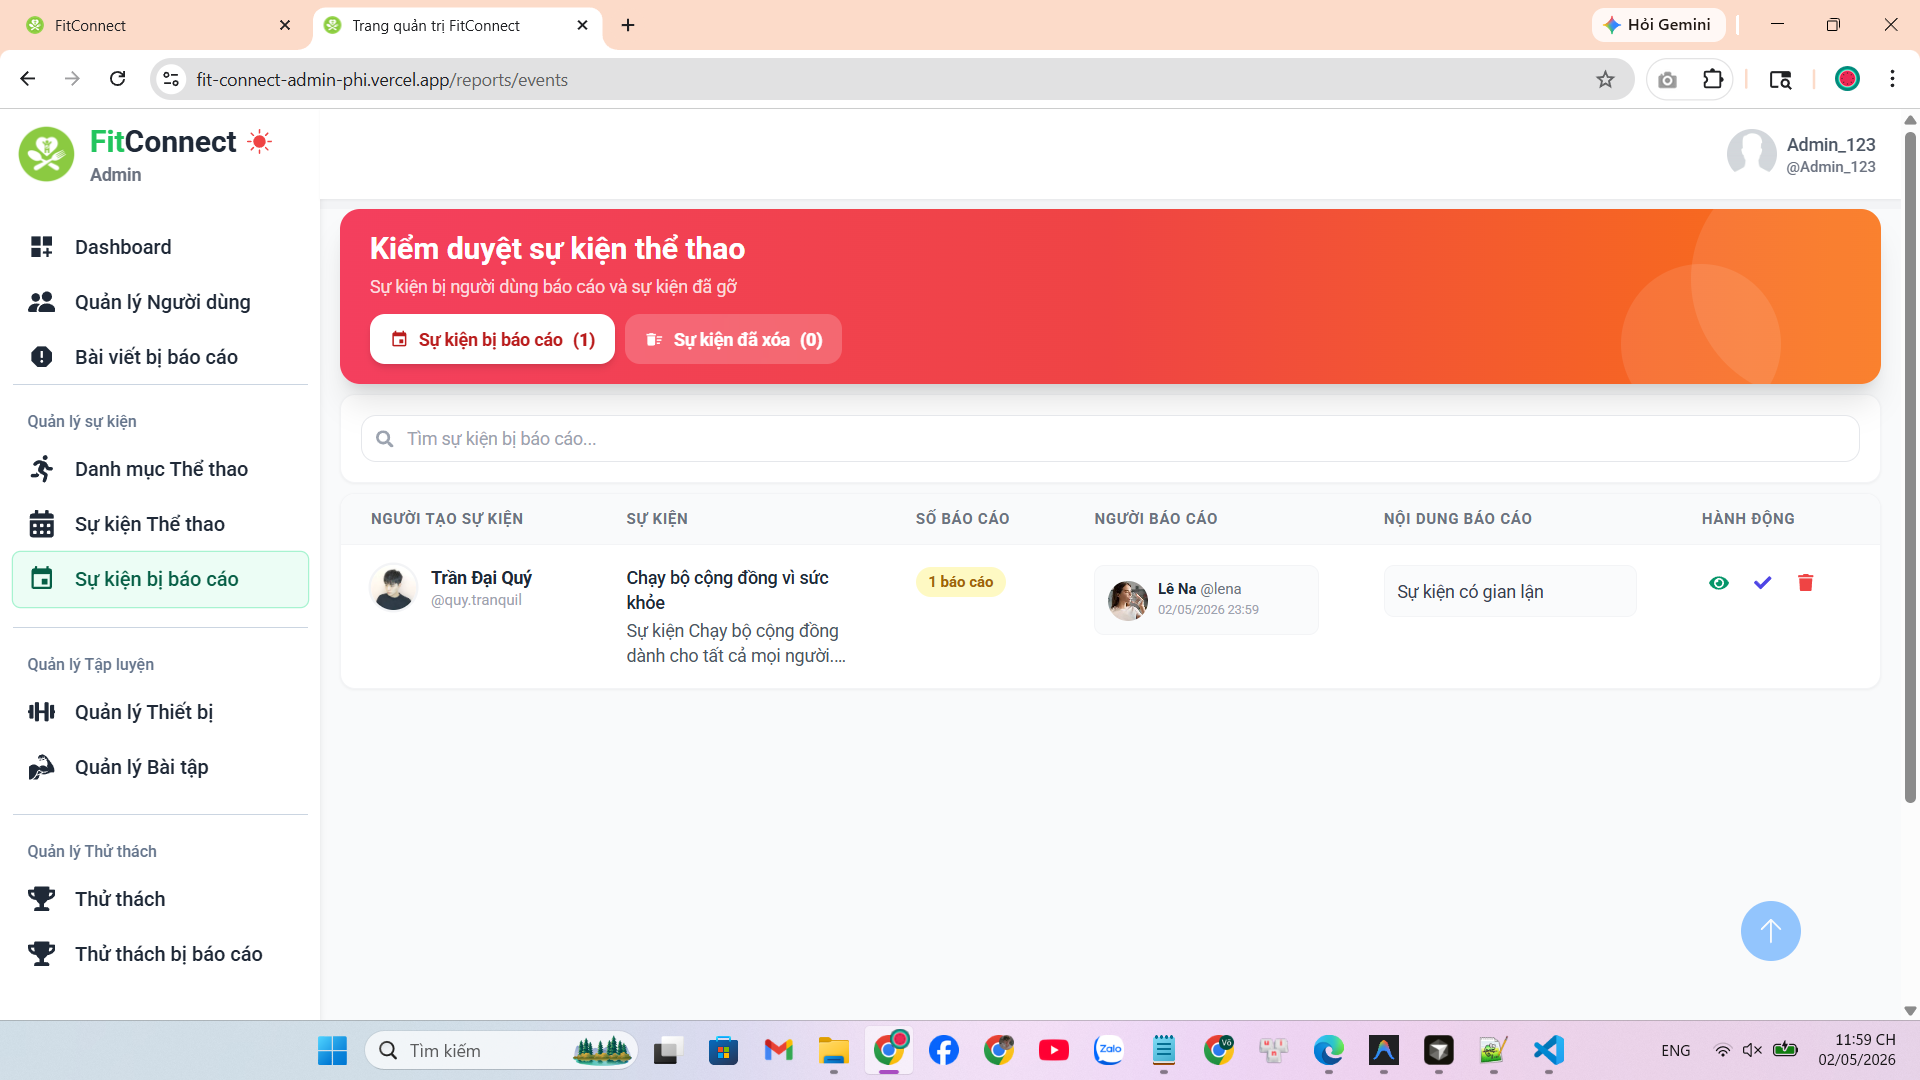
\includegraphics[width=0.60\textwidth]{Images/IMG/nhom9/kiemduyetsukienthethao/danhsachsukienbibaocaoadmin.png}
    \caption{Quản trị viên theo dõi danh sách các sự kiện thể thao bị báo cáo}
    \label{fig:impl_admin_event_mod_reported_list}
\end{figure}


    \item Để đảm bảo tính khách quan trước khi ra quyết định, Quản trị viên có thể xem chi tiết sự kiện kết hợp với nội dung khiếu nại thông qua một hộp thoại tích hợp.

\begin{figure}[H]
    \centering
    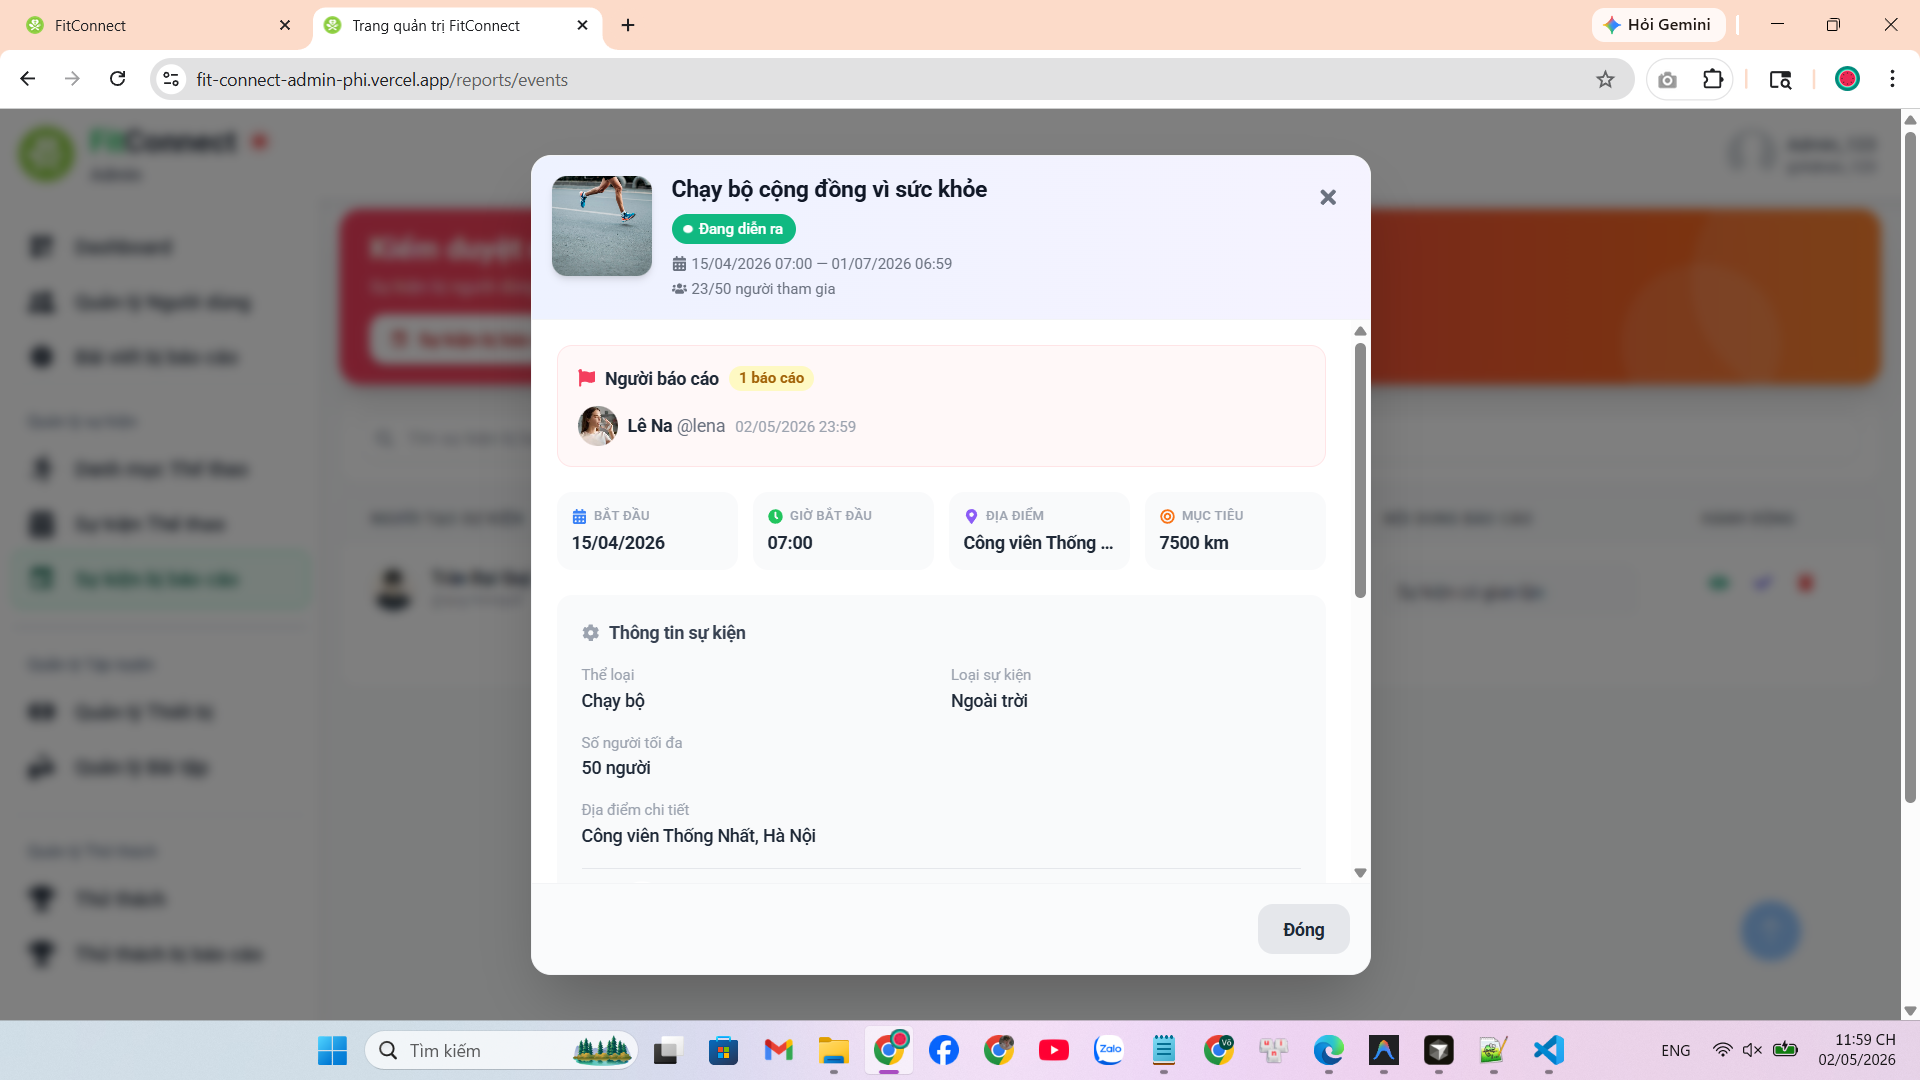
\includegraphics[width=0.60\textwidth]{Images/IMG/nhom9/kiemduyetsukienthethao/xemthongtinsukienbibaocao.png}
    \caption{Hệ thống hiển thị hộp thoại phân tích chi tiết sự kiện bị báo cáo}
    \label{fig:impl_admin_event_mod_detail}
\end{figure}


    \item Dựa trên xác minh, Admin quyết định \textbf{Giữ sự kiện} (bác bỏ báo cáo, xóa lịch sử khiếu nại) hoặc \textbf{Gỡ bỏ} (vô hiệu hóa sự kiện vi phạm, chuyển vào kho lưu trữ).

\begin{figure}[H]
    \centering
    \begin{subfigure}[b]{0.47\textwidth}
        \centering
        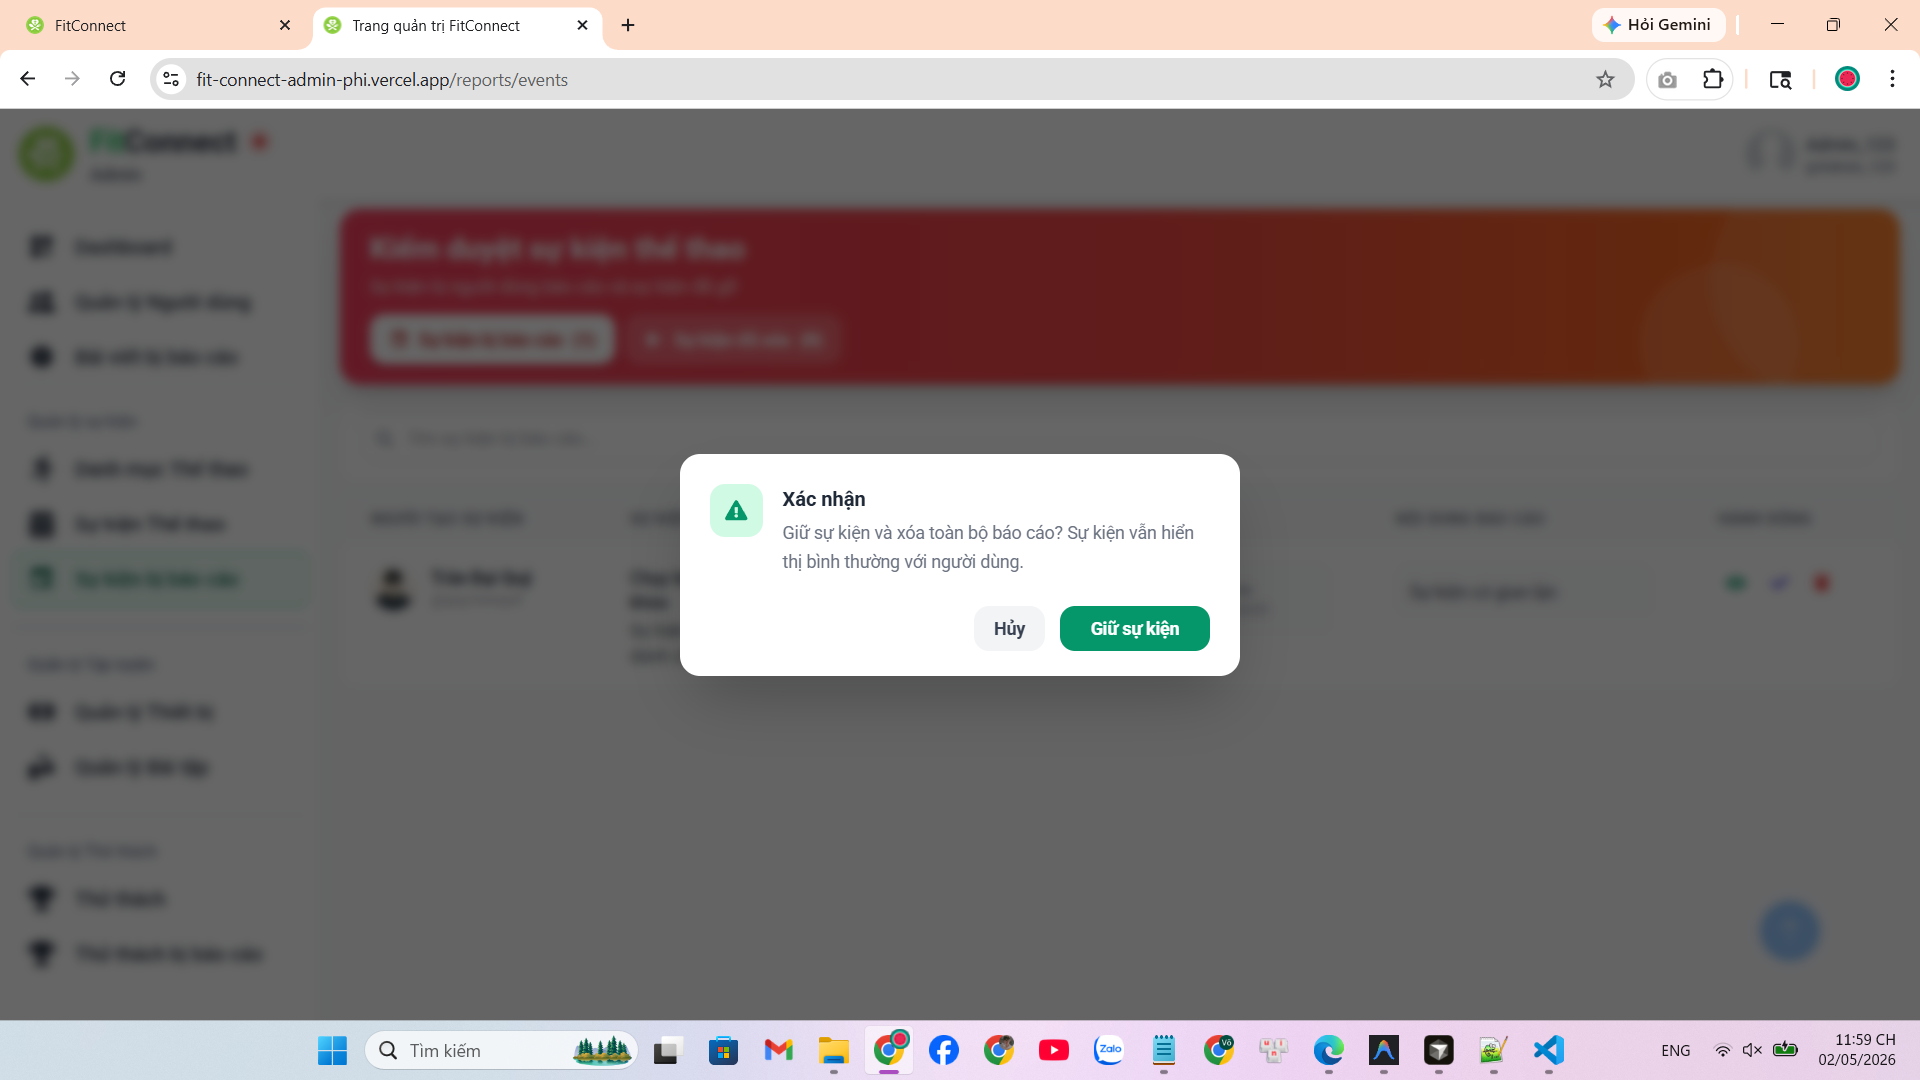
\includegraphics[width=\textwidth]{Images/IMG/nhom9/kiemduyetsukienthethao/modalgiusukien.png}
        \caption{Xác nhận giữ lại sự kiện hợp lệ}
        \label{fig:impl_admin_event_mod_keep}
    \end{subfigure}
    \hfill
    \begin{subfigure}[b]{0.47\textwidth}
        \centering
        
\includegraphics[width=\textwidth]{Images/IMG/nhom9/kiemduyetsukienthethao/adminxoasukien.png}
        \caption{Xác nhận gỡ bỏ sự kiện vi phạm}
        \label{fig:impl_admin_event_mod_remove}
    \end{subfigure}
    \vspace{0.3em}
    \caption{Hai hướng xử lý khi kiểm duyệt sự kiện bị báo cáo}
    \label{fig:impl_admin_event_mod_decision}
\end{figure}


    \item Việc gỡ bỏ sự kiện vi phạm sẽ khiến sự kiện ngay lập tức chuyển sang trạng thái hạn chế. Người dùng khi truy cập vào các sự kiện này sẽ nhận được thông báo về việc sự kiện đã bị quản trị viên gỡ bỏ và chuyển sang chế độ chỉ đọc, ngăn chặn mọi hành vi tương tác tiếp theo.
% \begin{figure}[H]
%     \centering
%     
\includegraphics[width=0.8\textwidth]{Images/IMG/nhom3/sukiensaukhixoa.png}
%     \vspace{1em}
%     \caption{Người dùng không thể thao tác với sự kiện đã bị gỡ bỏ do vi phạm}
%     \label{fig:impl_admin_event_mod_readonly_view}
% \end{figure}

    \item Mọi sự kiện bị gỡ bỏ đều được lưu trữ tại tab ``Đã xóa'' kèm thời điểm và nội dung vi phạm. Quản trị viên có thể khôi phục sự kiện bất kỳ lúc nào nếu cần thiết.

\begin{figure}[H]
    \centering
    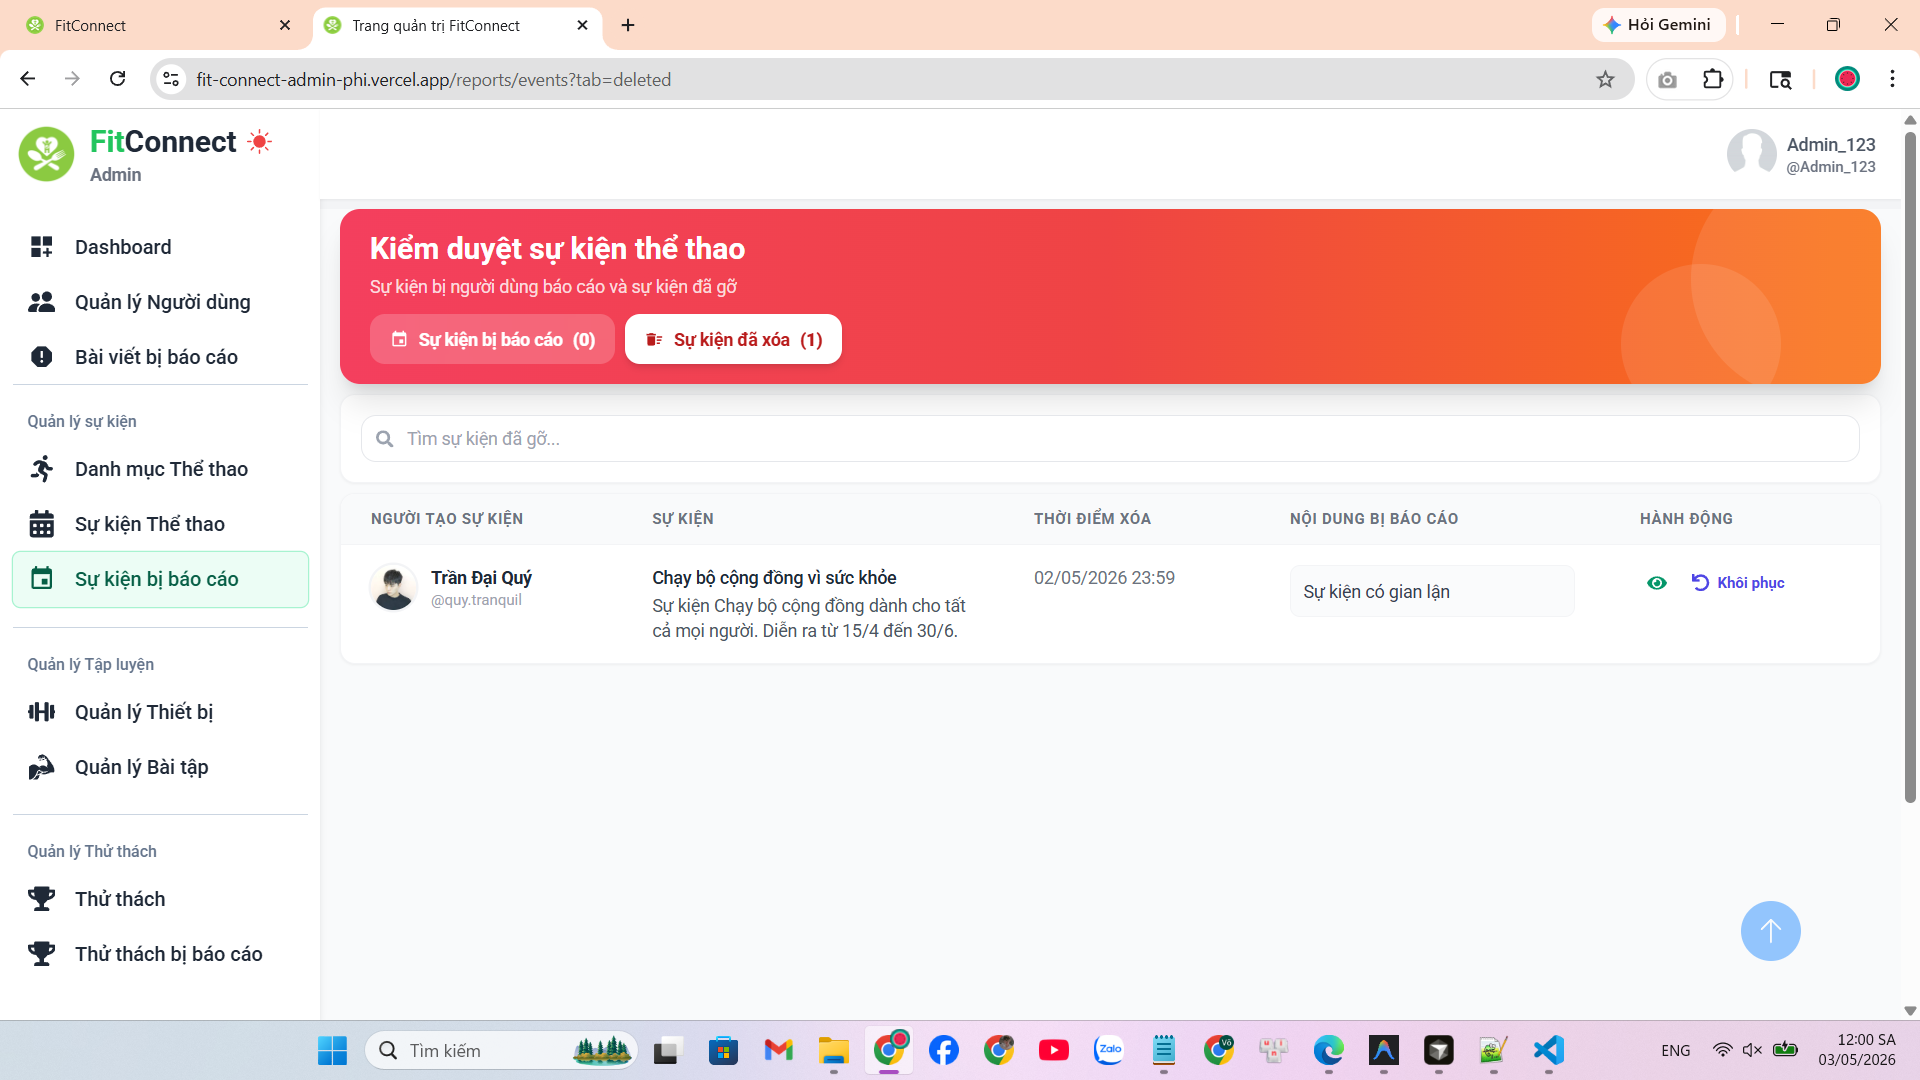
\includegraphics[width=0.60\textwidth]{Images/IMG/nhom9/kiemduyetsukienthethao/danhsachsukiendaxoa.png}
    \caption{Danh sách sự kiện đã bị gỡ bỏ do vi phạm, cho phép xem xét và khôi phục}
    \label{fig:impl_admin_event_mod_deleted_list}
\end{figure}

\end{itemize}

\subsubsection{Luồng thao tác quản lý thiết bị}
\begin{itemize}
    \item Trang Quản lý Thiết bị cho phép Quản trị viên xem và kiểm soát danh sách các loại thiết bị, dụng cụ hỗ trợ tập luyện có sẵn trong hệ thống (như xà đơn, ghế tập, tạ tay, tạ đòn, dây kháng lực,...). Giao diện hiển thị trực quan dưới dạng thẻ (card), cung cấp các thông tin cơ bản gồm hình ảnh minh họa, tên tiếng Việt, tên tiếng Anh, và trạng thái hiện tại (Hoạt động/Đã ẩn).

\begin{figure}[H]
    \centering
    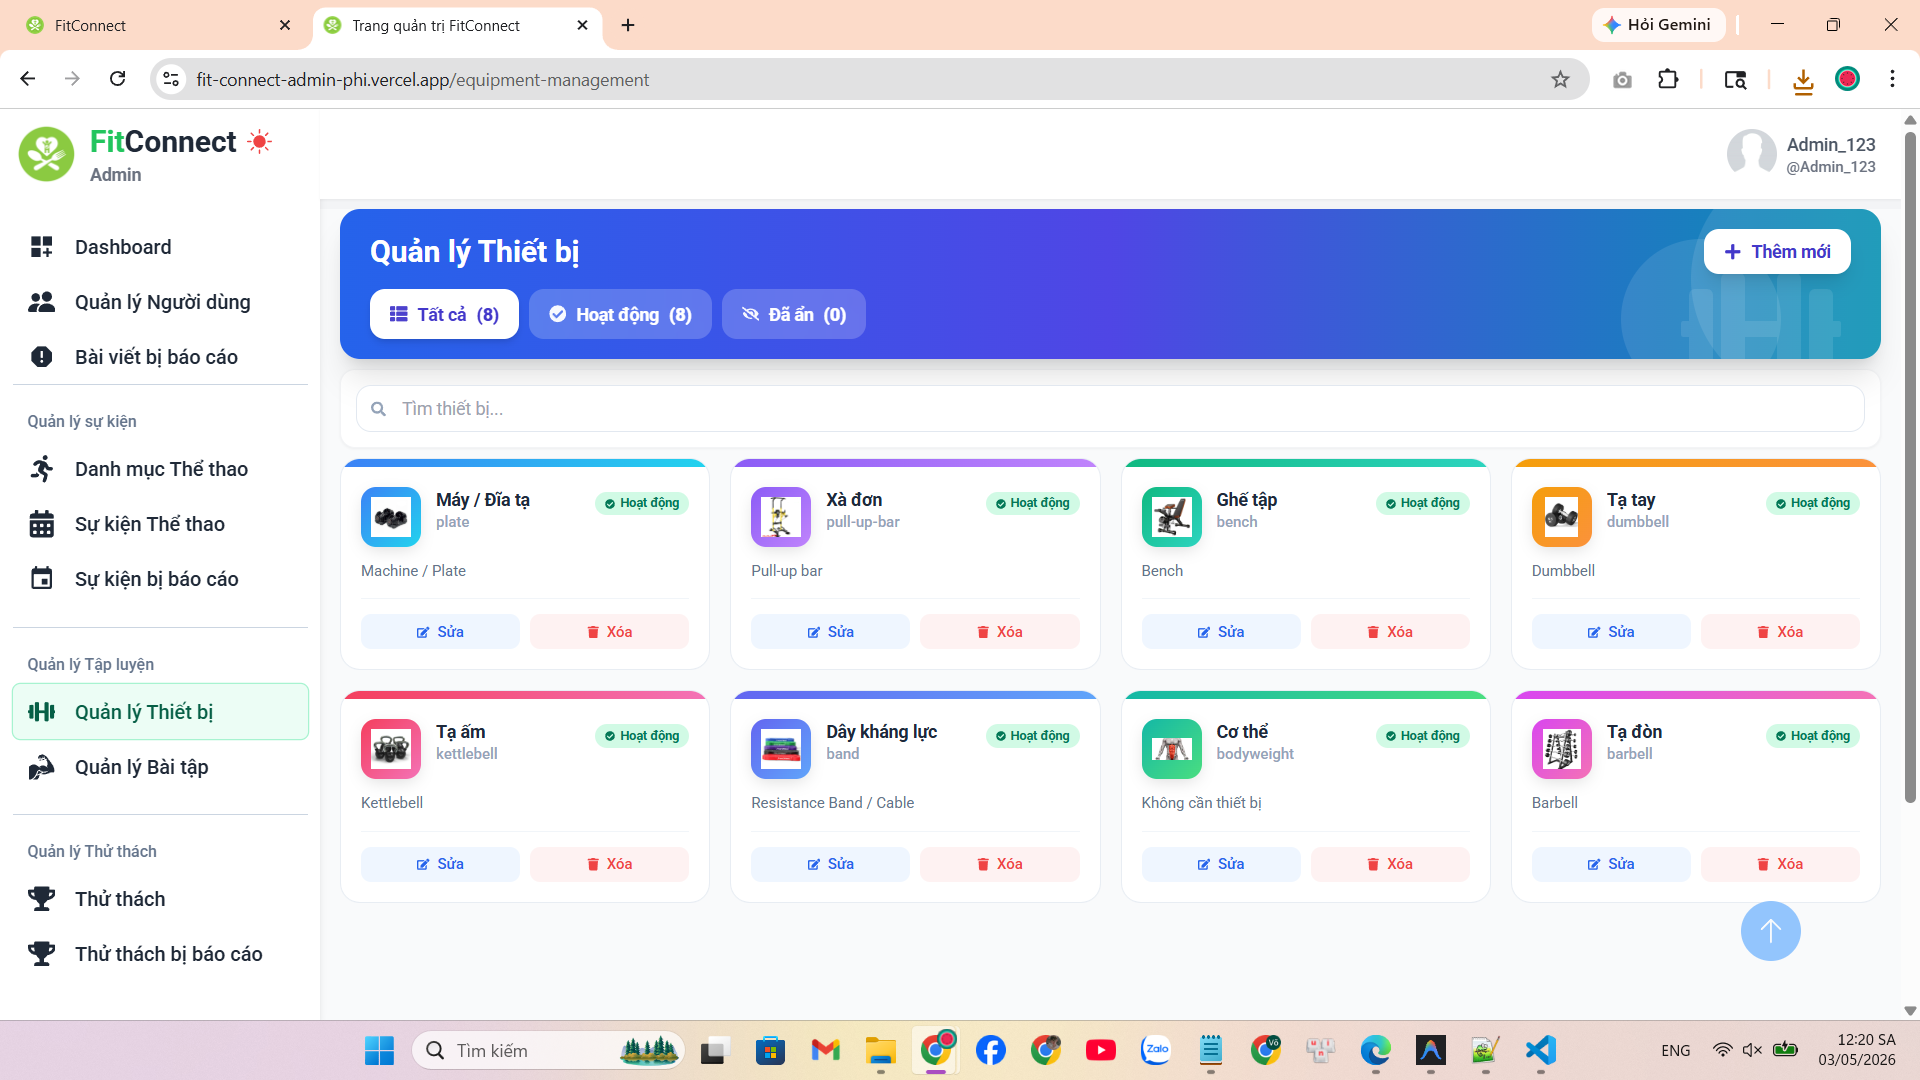
\includegraphics[width=0.60\textwidth]{Images/IMG/nhom9/quanlythietbi/danhsachthietbi.png}
    \caption{Giao diện danh sách các thiết bị tập luyện do hệ thống quản lý}
    \label{fig:impl_admin_equipment_list}
\end{figure}


    \item Để làm phong phú thêm cơ sở dữ liệu hỗ trợ tập luyện, Quản trị viên có thể sử dụng chức năng ``Thêm mới''. Hộp thoại Thêm thiết bị yêu cầu cung cấp hình ảnh minh họa định dạng chuẩn, tên gọi song ngữ (Anh - Việt), mô tả ngắn gọn và công tắc kích hoạt trạng thái hoạt động ngay lập tức.

\begin{figure}[H]
    \centering
    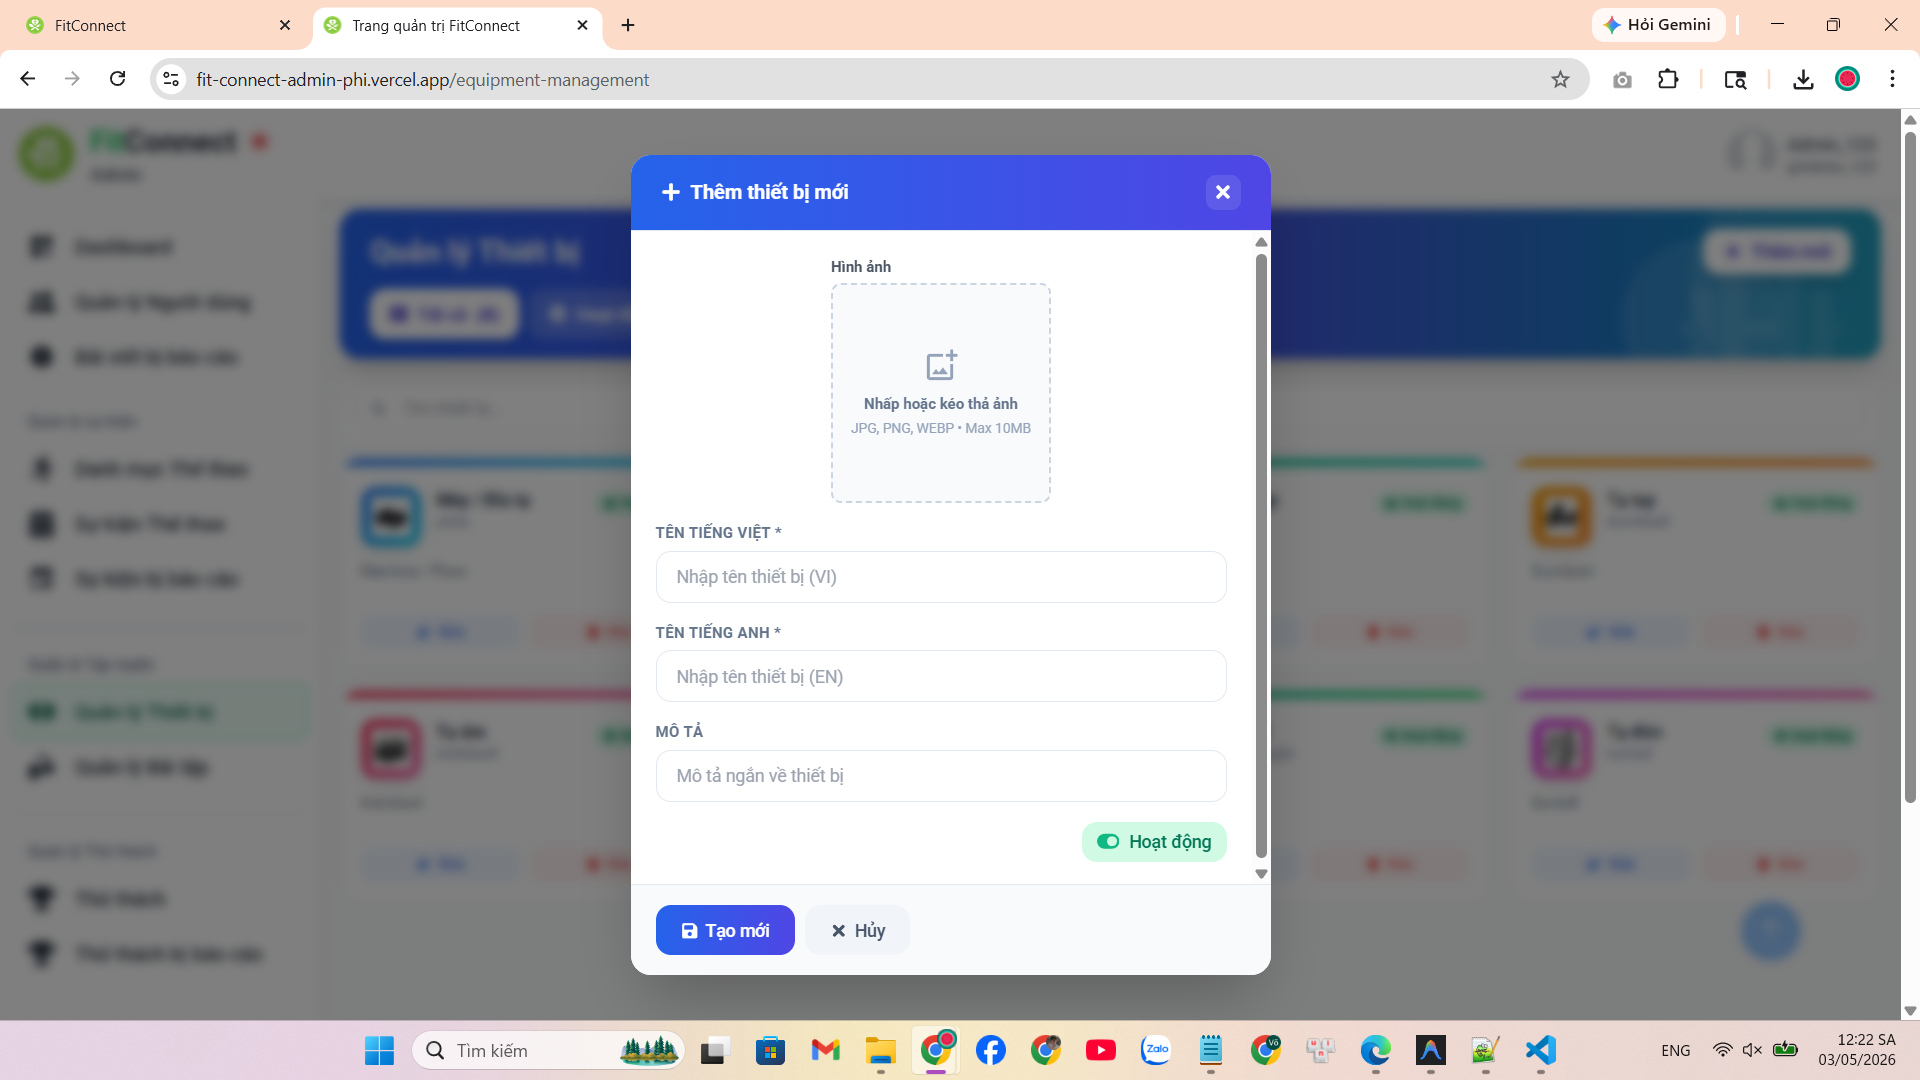
\includegraphics[width=0.60\textwidth]{Images/IMG/nhom9/quanlythietbi/themmoithietbi.png}
    \caption{Hệ thống cung cấp hộp thoại tạo mới thiết bị tập luyện}
    \label{fig:impl_admin_equipment_add}
\end{figure}


    \item Khi có sự thay đổi về thông tin (ví dụ: cần cập nhật hình ảnh rõ nét hơn hoặc bổ sung mô tả), tính năng ``Sửa'' cho phép Admin thực hiện cập nhật dựa trên form dữ liệu đã được điền sẵn. Mọi thay đổi đều được hệ thống lưu trữ đồng bộ, giúp dữ liệu thiết bị luôn chính xác khi liên kết với các bài tập.

\begin{figure}[H]
    \centering
    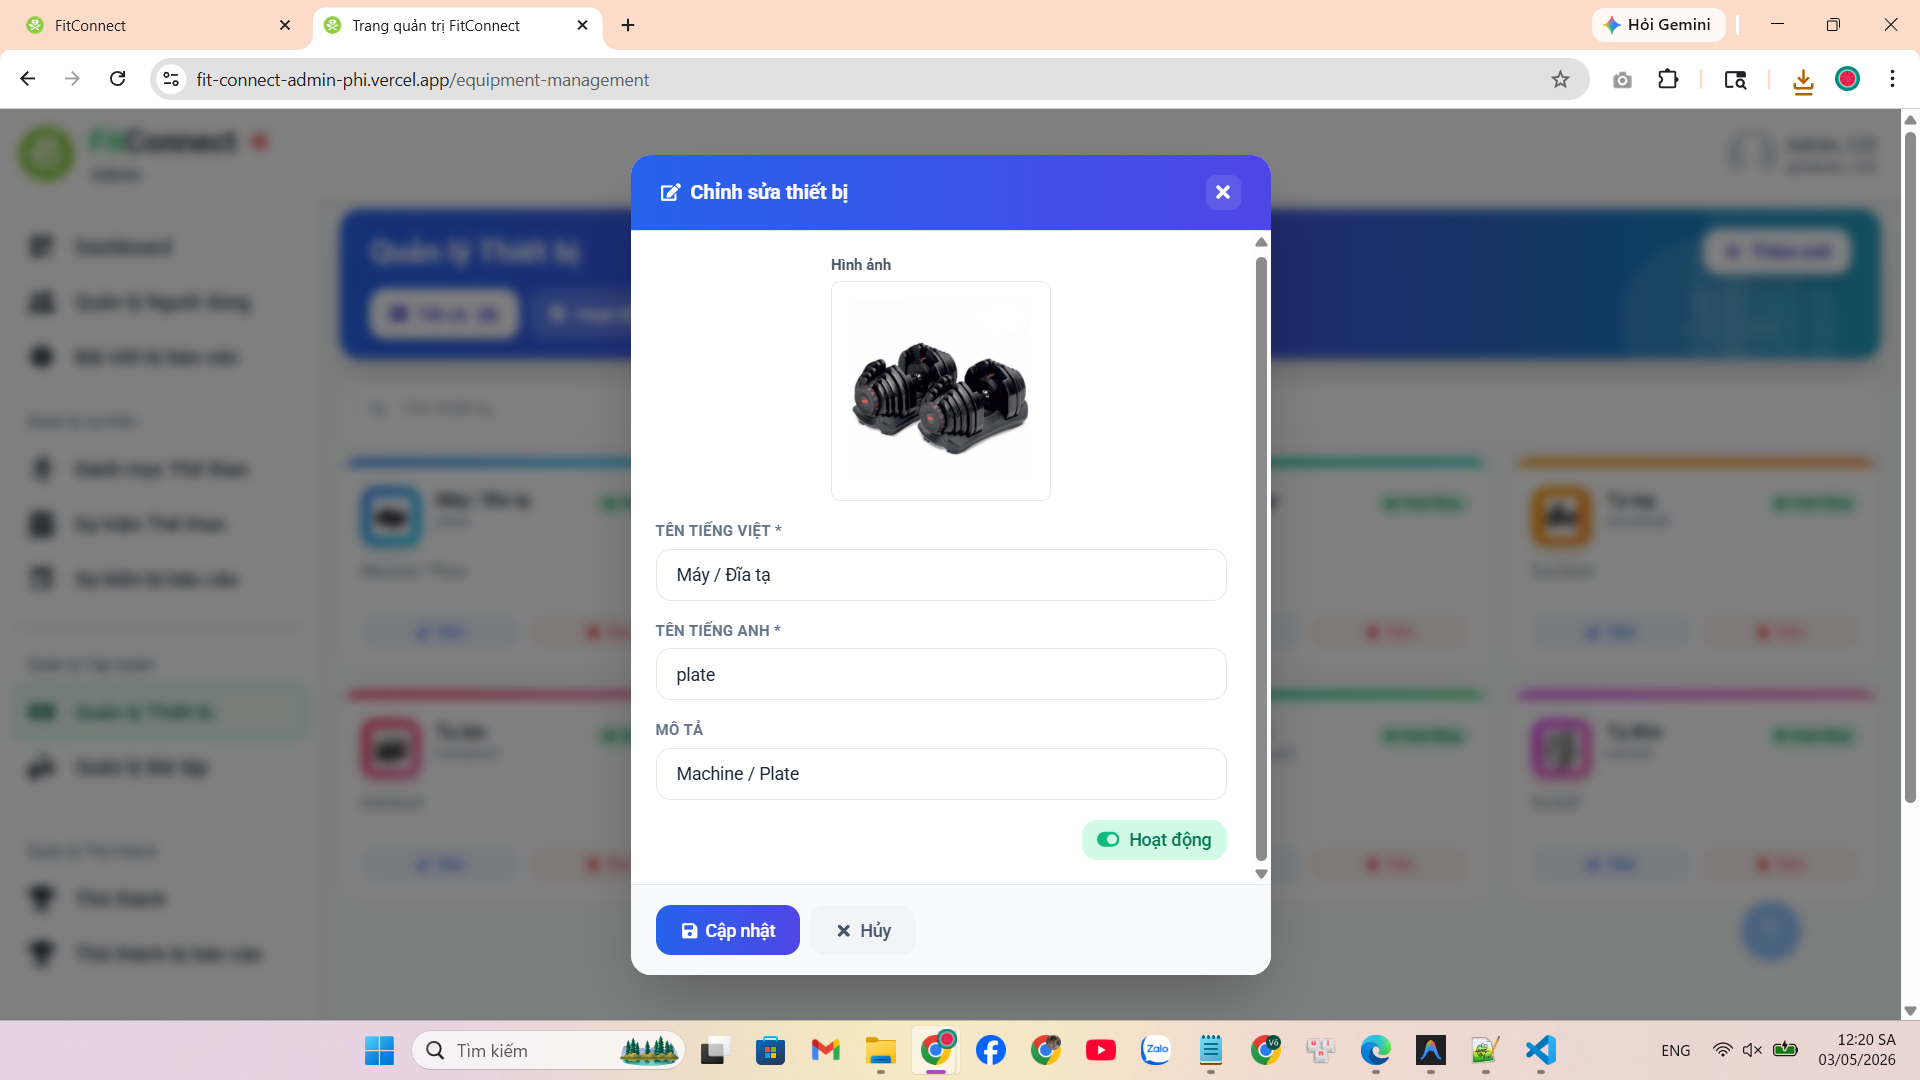
\includegraphics[width=0.60\textwidth]{Images/IMG/nhom9/quanlythietbi/chinhsuathietbi.png}
    \caption{Hộp thoại chỉnh sửa thông tin thiết bị với dữ liệu được điền sẵn}
    \label{fig:impl_admin_equipment_edit}
\end{figure}

\end{itemize}

\subsubsection{Luồng thao tác quản lý bài tập}
\begin{itemize}
    \item Trang Quản lý Bài tập là trung tâm kiểm soát toàn bộ cơ sở dữ liệu các động tác tập luyện (exercises). Giao diện cung cấp danh sách chi tiết dưới dạng bảng, phân loại theo loại hình (Sức mạnh, Tim mạch, Giãn cơ, Bật nhảy), độ khó, cấu trúc sets/reps, nhóm cơ chịu tác động và các thiết bị đi kèm. Tính năng bộ lọc (Filter) thông minh theo Nhóm cơ hoặc Thiết bị giúp Admin dễ dàng tra cứu khối lượng dữ liệu khổng lồ.

\begin{figure}[H]
    \centering
    
\includegraphics[width=0.60\textwidth]{Images/IMG/nhom9/quanlybaitap/danhsachbaitap.png}
    \caption{Giao diện tổng quan danh sách bài tập được phân loại chi tiết}
    \label{fig:impl_admin_exercise_list}
\end{figure}


    \item Quy trình thêm một bài tập mới đòi hỏi sự chính xác cao về chuyên môn. Hộp thoại ``Thêm bài tập mới'' không chỉ thu thập thông tin cơ bản (tên song ngữ, phân loại), mà còn yêu cầu thiết lập các cấu hình phức tạp: lựa chọn đa dạng các nhóm cơ và thiết bị bằng thẻ (tags), nhập hướng dẫn từng bước chi tiết, cung cấp liên kết video minh họa, cấu hình nhịp tập (số giây/rep, thời gian nghỉ) và đặc biệt là bảng thông số Set tập mặc định. Bảng này hỗ trợ tự động gợi ý chỉ số luyện tập tiêu chuẩn dựa trên mức độ khó (Dễ, Trung bình, Khó) với các giá trị về số rep, mức tạ và năng lượng Kcal tiêu thụ ước tính.

\begin{figure}[H]
    \centering
    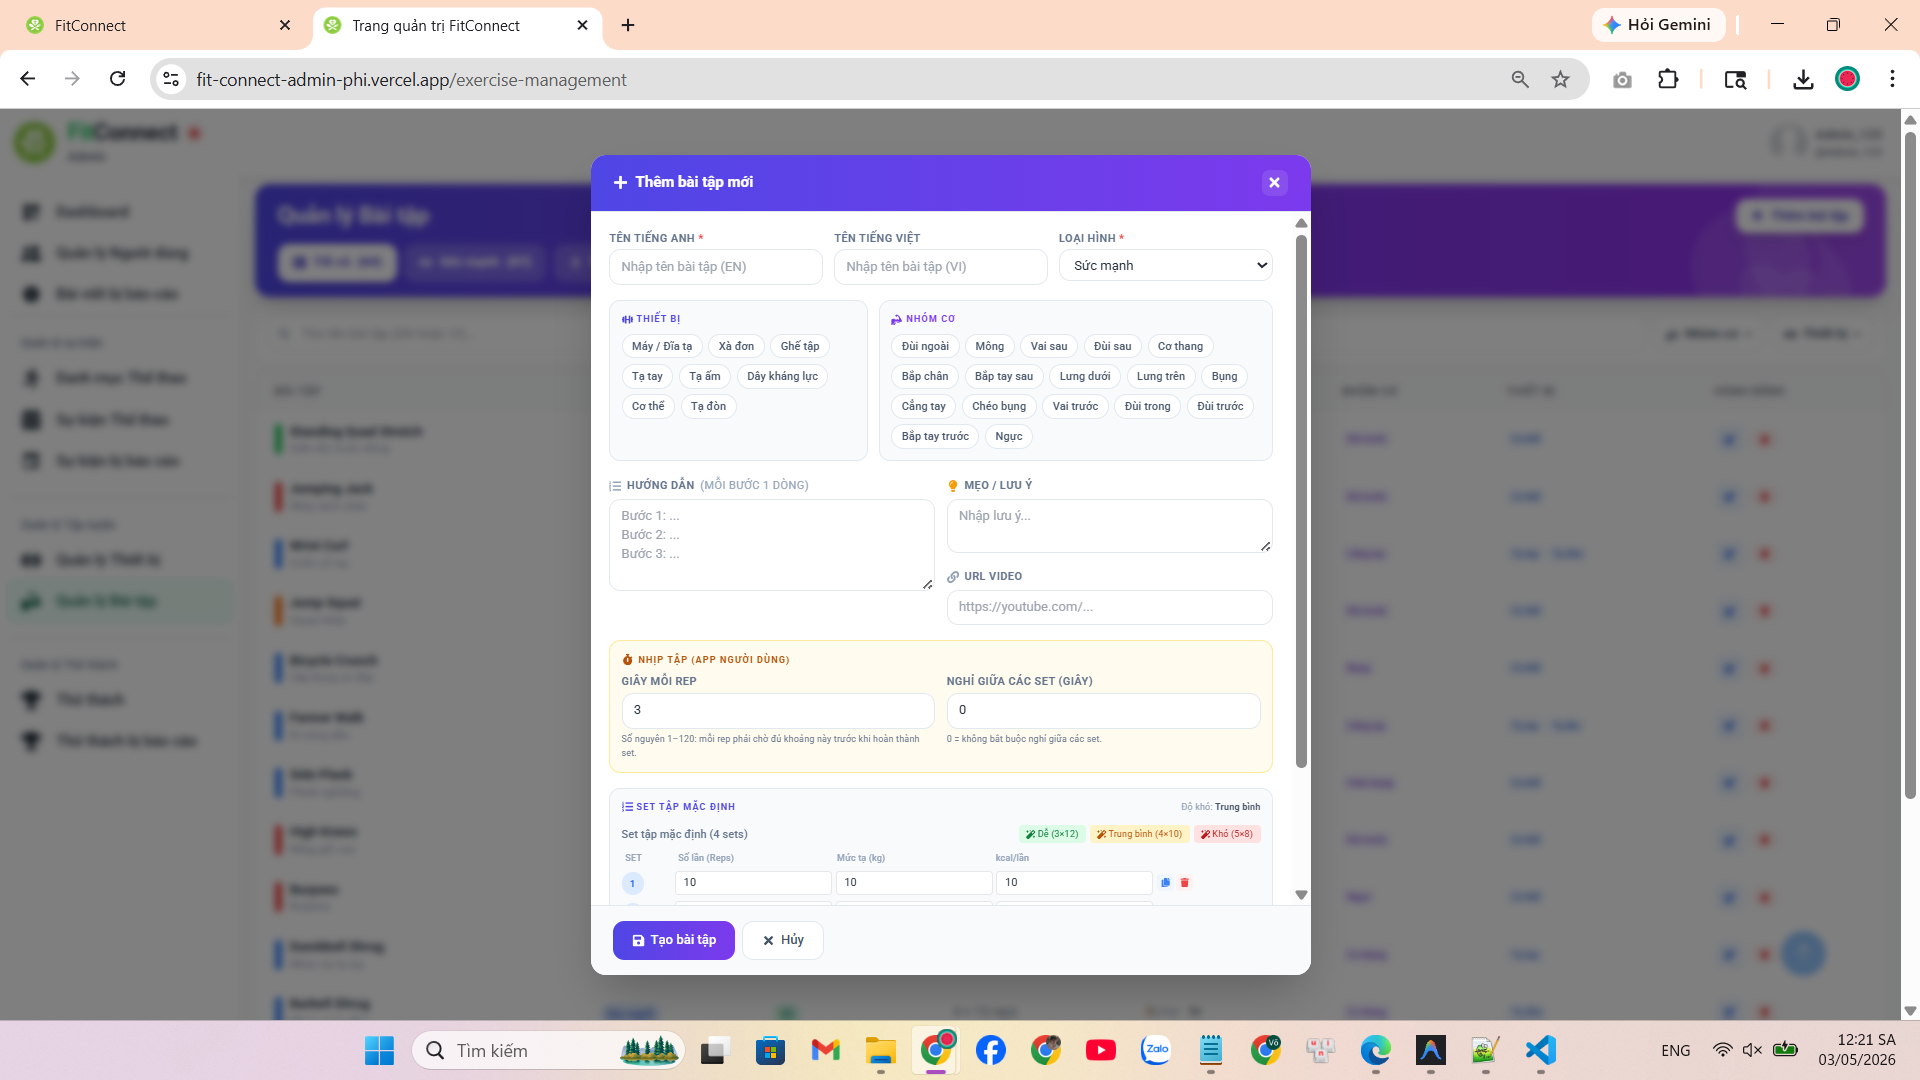
\includegraphics[width=0.60\textwidth]{Images/IMG/nhom9/quanlybaitap/themmoibaitap.png}
    \caption{Hộp thoại thêm mới bài tập với hệ thống thiết lập thông số chuyên sâu}
    \label{fig:impl_admin_exercise_add}
\end{figure}


    \item Trong trường hợp cần tinh chỉnh hướng dẫn tập luyện hoặc cập nhật chỉ số Kcal để phù hợp hơn với thực tế, chức năng chỉnh sửa cung cấp môi trường làm việc trực quan. Quản trị viên dễ dàng thêm/bớt nhóm cơ tác động hoặc sửa đổi lại cấu trúc từng set tập trước khi lưu cập nhật. Dữ liệu này sẽ làm nền tảng cốt lõi cho tính năng tự động thiết kế lộ trình tập luyện thông minh của người dùng (Smart Workout).

\begin{figure}[H]
    \centering
    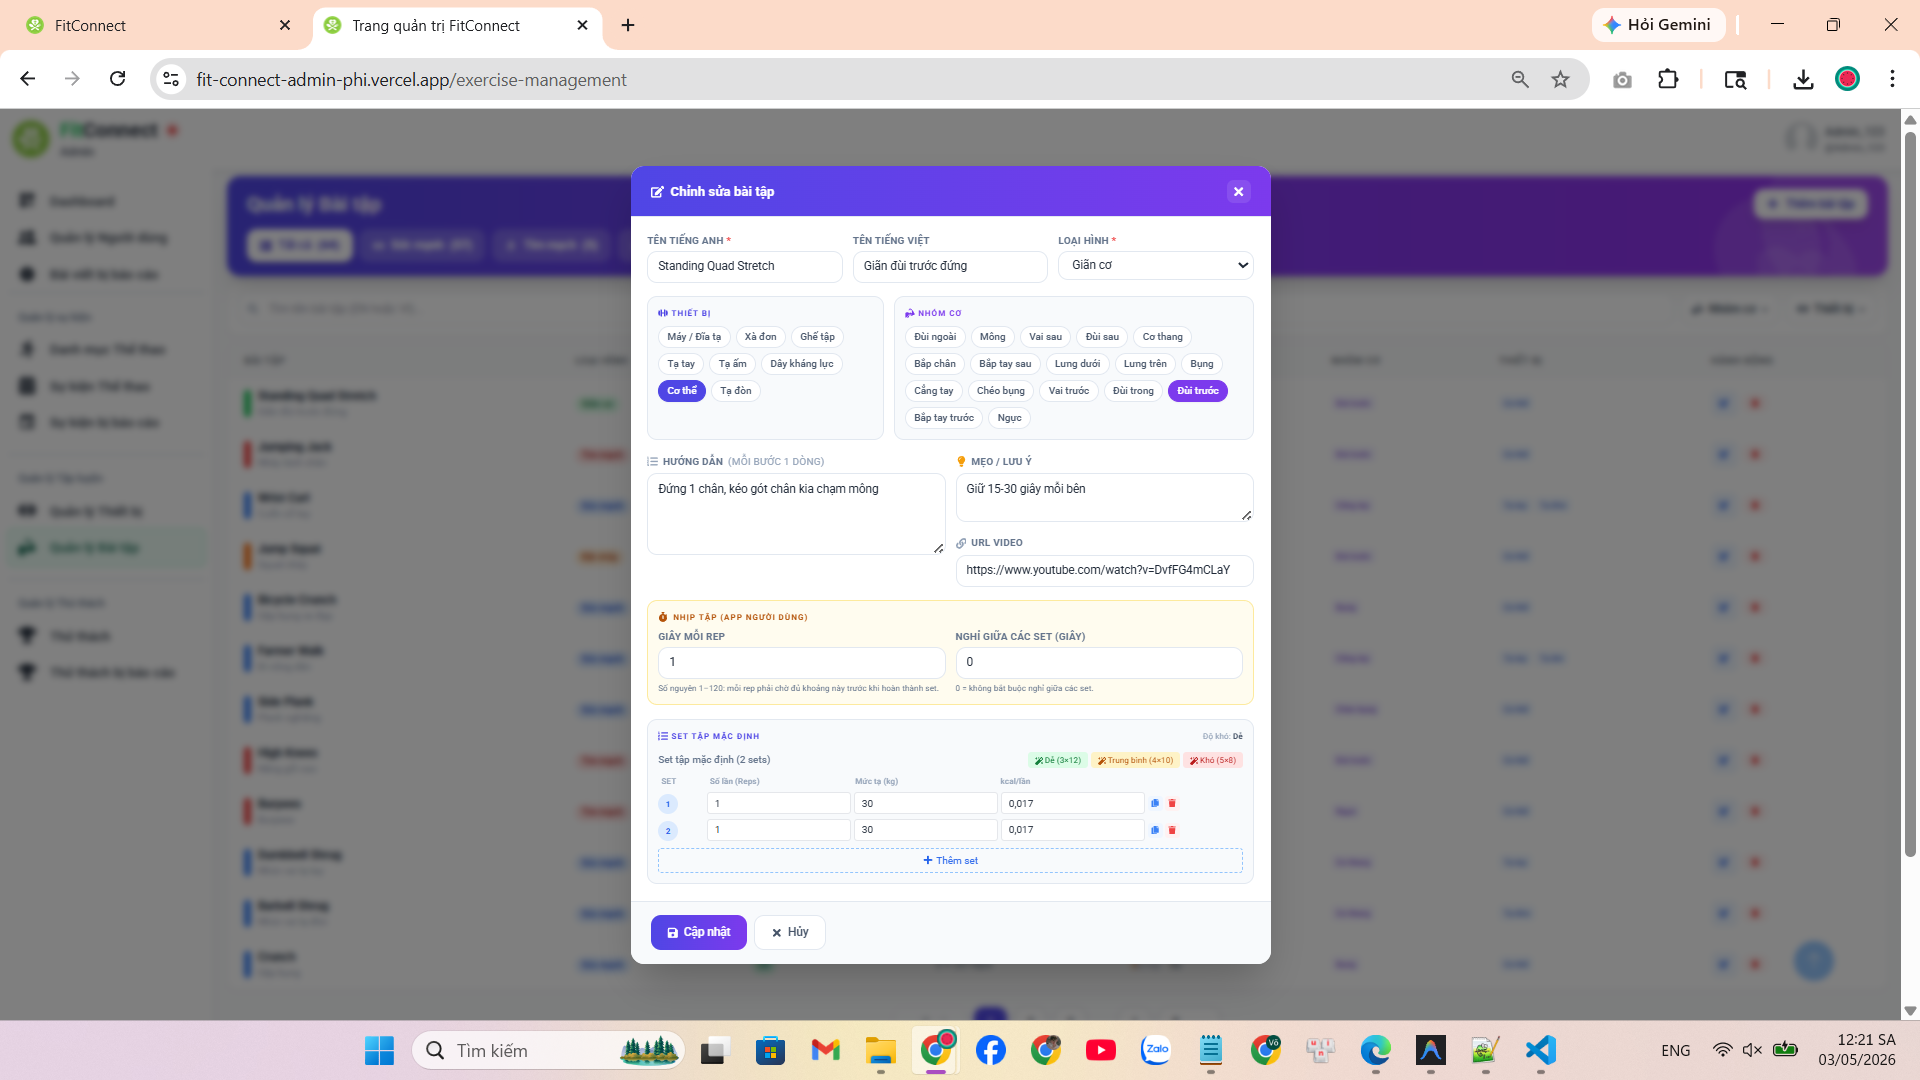
\includegraphics[width=0.60\textwidth]{Images/IMG/nhom9/quanlybaitap/chinhsuabaitap.png}
    \caption{Giao diện chỉnh sửa cho phép tinh chỉnh lại các thông số kỹ thuật của bài tập}
    \label{fig:impl_admin_exercise_edit}
\end{figure}

\end{itemize}

\subsubsection{Luồng thao tác quản lý thử thách}
\begin{itemize}
    \item Hệ thống cung cấp cho Quản trị viên giao diện quản lý tập trung toàn bộ các thử thách cộng đồng. Tại đây, Admin có thể theo dõi danh sách các thử thách đang hoạt động, bao gồm thông tin về loại thử thách (Sức mạnh, Tim mạch,...), số lượng người tham gia, thời gian bắt đầu và kết thúc, cùng trạng thái hiện tại của từng thử thách.

\begin{figure}[H]
    \centering
    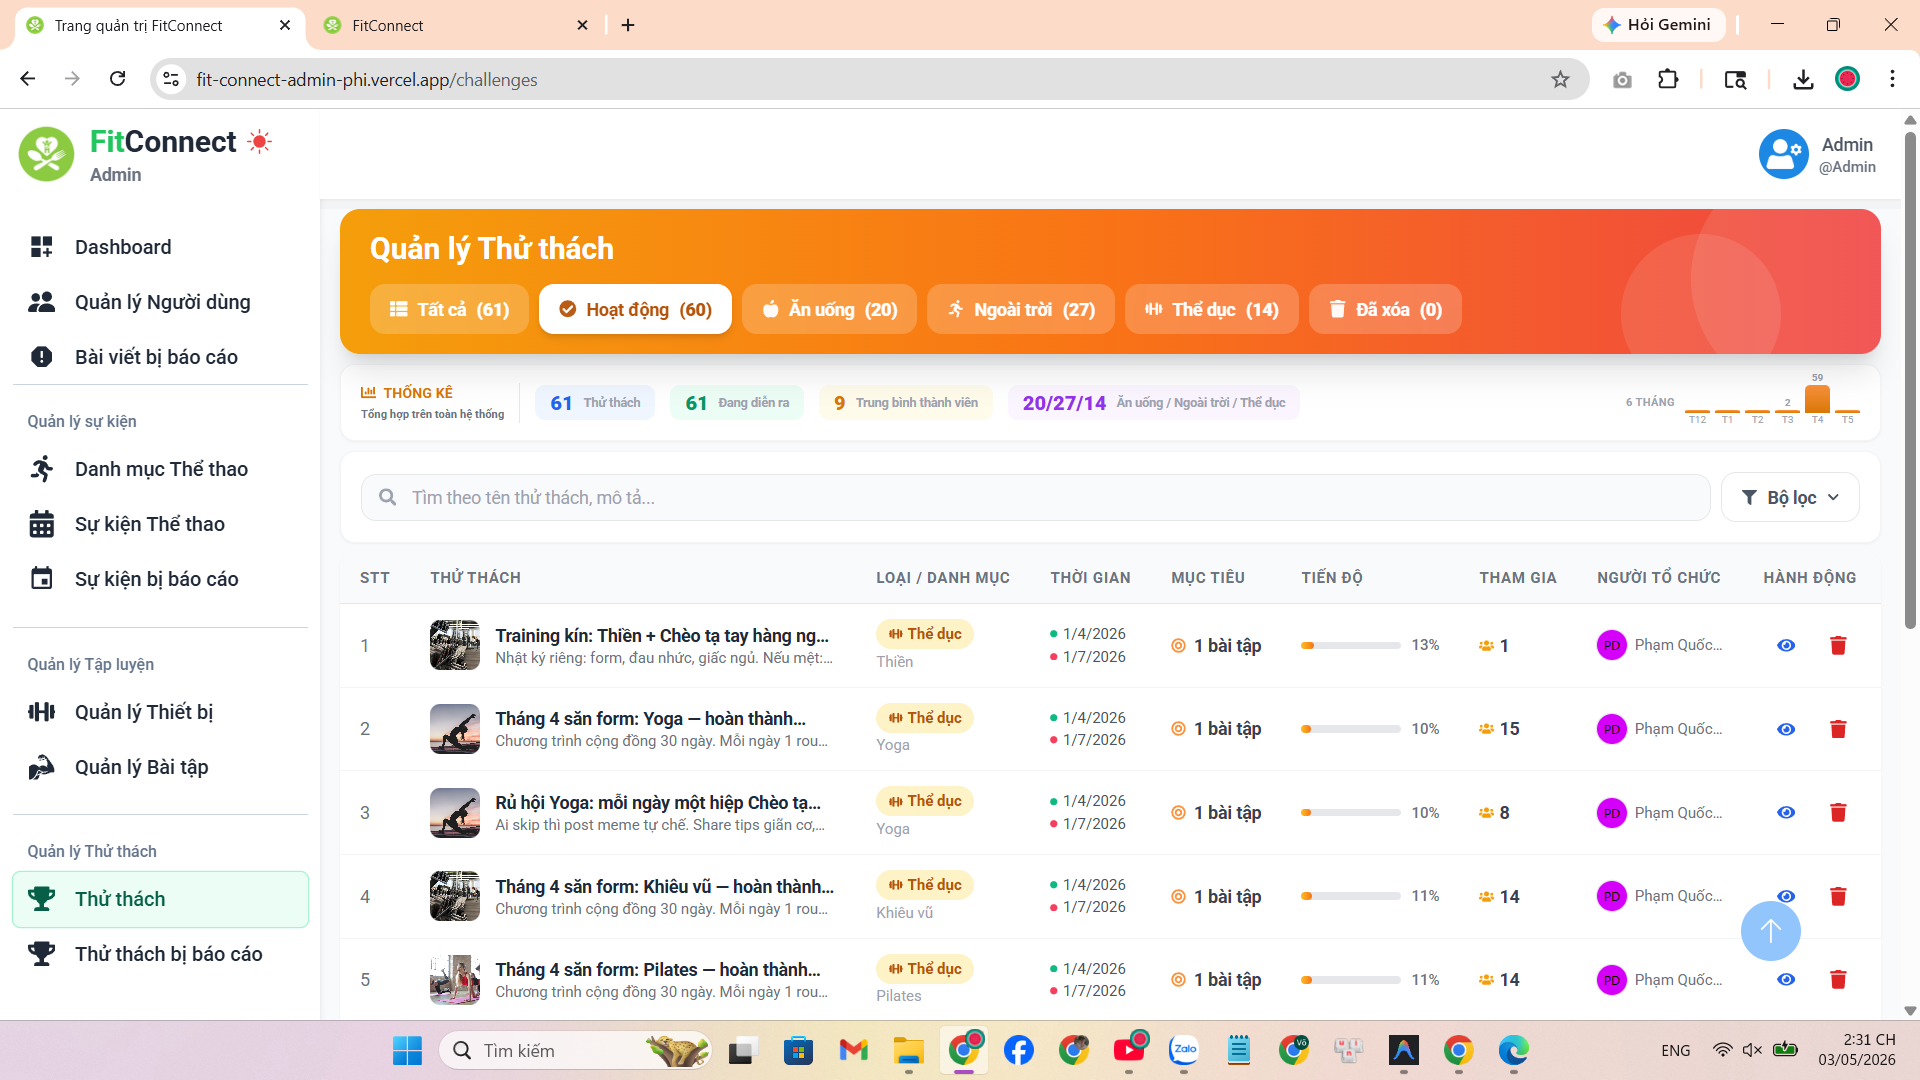
\includegraphics[width=0.60\textwidth]{Images/IMG/nhom9/quanlythuthach/danhsachthuthach.png}
    \caption{Quản trị viên xem danh sách tổng hợp các thử thách trên hệ thống}
    \label{fig:impl_admin_challenge_list}
\end{figure}


    \item Để đánh giá nội dung và tính phù hợp của thử thách, Quản trị viên có thể xem chi tiết thông tin thông qua hộp thoại phân tích. Hệ thống hiển thị đầy đủ mô tả, mục tiêu cần đạt được (ví dụ: số kcal cần đốt, quãng đường cần chạy) và danh sách các bài tập liên quan nếu có.

\begin{figure}[H]
    \centering
    
\includegraphics[width=0.60\textwidth]{Images/IMG/nhom9/quanlythuthach/xemthongtinthuthach.png}
    \caption{Hệ thống hiển thị hộp thoại chi tiết thông tin thử thách}
    \label{fig:impl_admin_challenge_detail}
\end{figure}


    \item Trong quá trình vận hành, nếu phát hiện thử thách có nội dung không phù hợp hoặc vi phạm chính sách nền tảng, Quản trị viên có quyền thực hiện thao tác vô hiệu hóa. Trước khi thực hiện, hệ thống sẽ hiển thị hộp thoại xác nhận để đảm bảo quyết định được cân nhắc kỹ lưỡng.

\begin{figure}[H]
    \centering
    
\includegraphics[width=0.60\textwidth]{Images/IMG/nhom9/quanlythuthach/xoathuthach.png}
    \caption{Hệ thống hiển thị hộp thoại xác nhận vô hiệu hóa thử thách}
    \label{fig:impl_admin_challenge_delete_confirm}
\end{figure}


    \item Sau khi vô hiệu hóa, thử thách chuyển sang chế độ chỉ đọc (người dùng xem được lịch sử nhưng không tương tác thêm). Các thử thách đã xóa được lưu tại kho riêng và có thể khôi phục để người dùng tiếp tục tham gia.

\begin{figure}[H]
    \centering
    \begin{subfigure}[b]{0.47\textwidth}
        \centering
        
\includegraphics[width=\textwidth]{Images/IMG/nhom9/quanlythuthach/danhsachthuthachdaxoa.png}
        \caption{Danh sách thử thách đã vô hiệu hóa}
        \label{fig:impl_admin_challenge_deleted_list}
    \end{subfigure}
    \hfill
    \begin{subfigure}[b]{0.47\textwidth}
        \centering
        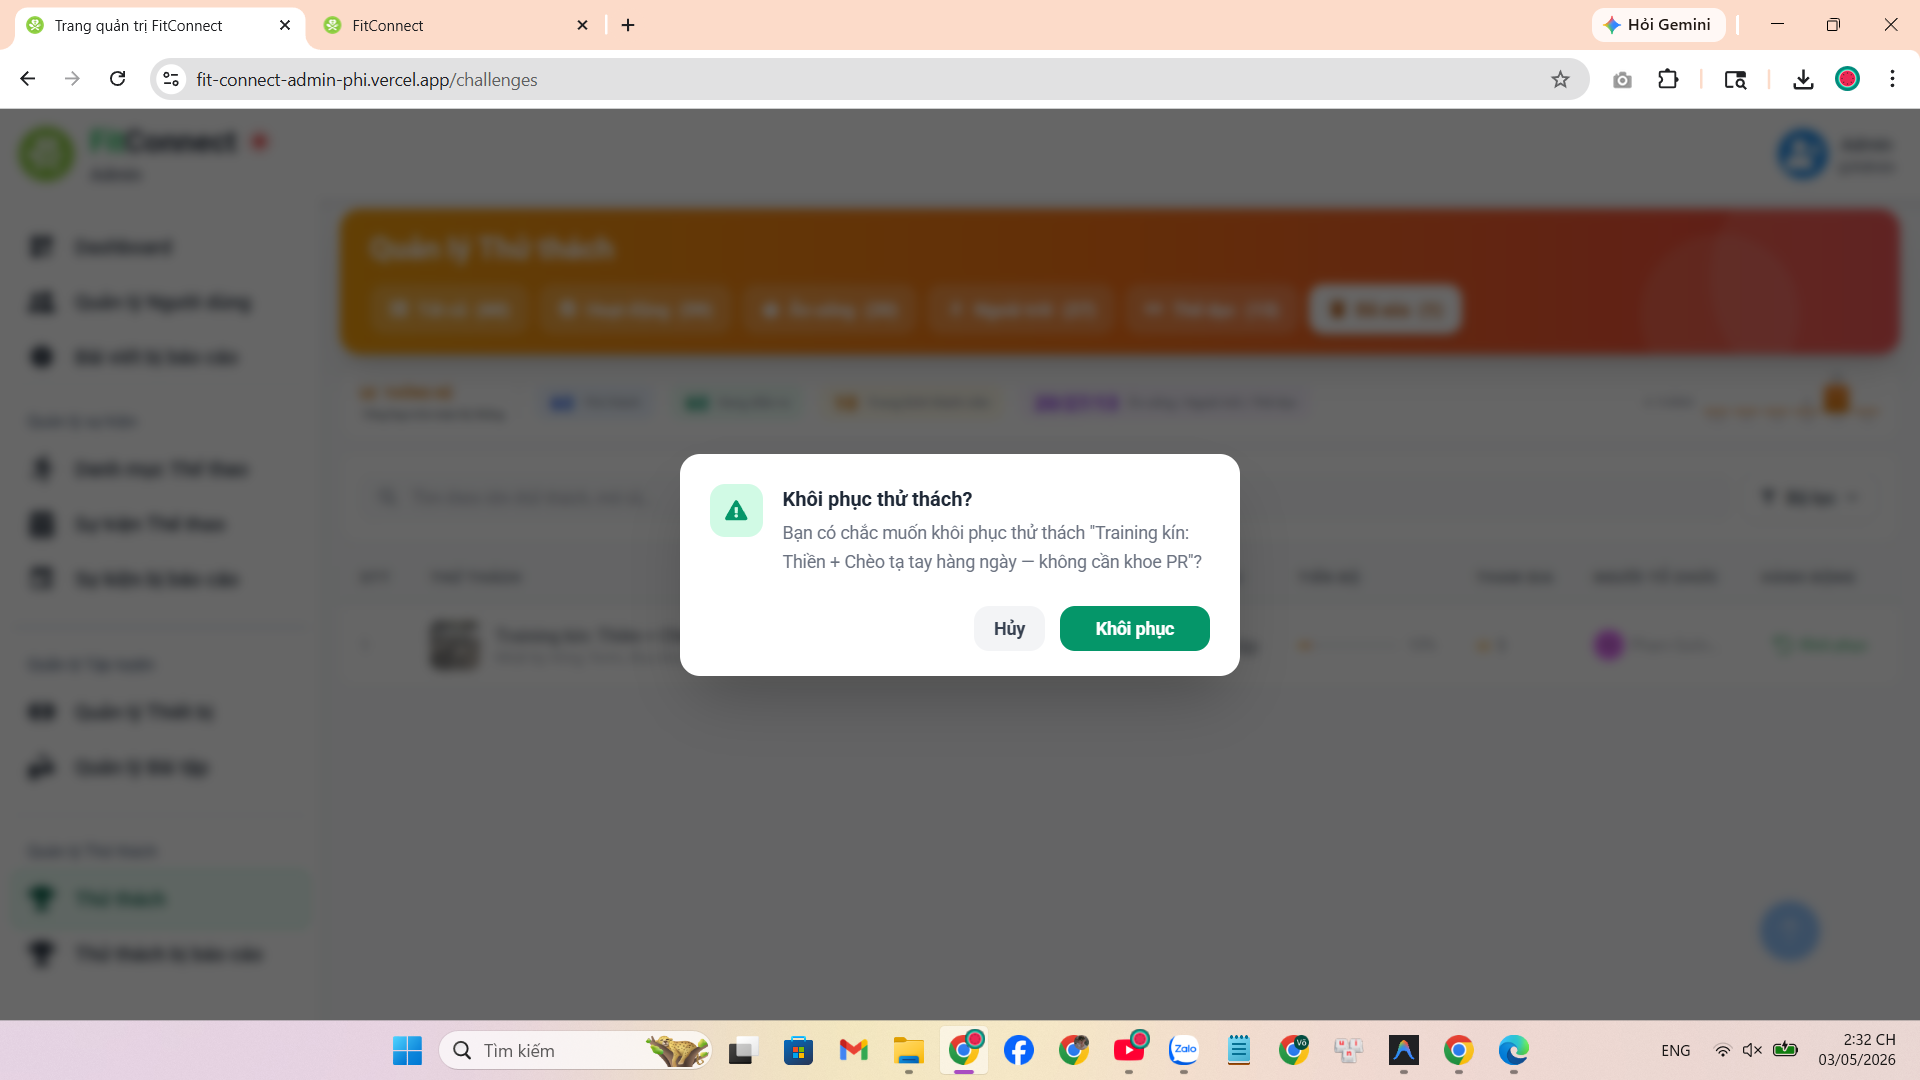
\includegraphics[width=\textwidth]{Images/IMG/nhom9/quanlythuthach/khoiphucthuthach.png}
        \caption{Xác nhận khôi phục thử thách}
        \label{fig:impl_admin_challenge_restore_confirm}
    \end{subfigure}
    \vspace{0.3em}
    \caption{Kho lưu trữ thử thách đã xóa và quy trình khôi phục}
    \label{fig:impl_admin_challenge_trash}
\end{figure}

\end{itemize}

\subsubsection{Luồng thao tác kiểm duyệt Thử thách cộng đồng}
\begin{itemize}
    \item Quy trình kiểm duyệt thử thách bắt đầu từ sự chủ động của cộng đồng người dùng. Khi phát hiện một thử thách có dấu hiệu gian lận, nội dung phản cảm hoặc không phù hợp với tiêu chuẩn sức khỏe, người dùng có thể gửi báo cáo vi phạm trực tiếp kèm theo lý do chi tiết.

\begin{figure}[H]
    \centering
    
\includegraphics[width=0.60\textwidth]{Images/IMG/nhom9/kiemduyetthuthach/baocaothuthach.png}
    \caption{Người dùng thực hiện báo cáo vi phạm đối với một thử thách cộng đồng}
    \label{fig:impl_admin_challenge_mod_report}
\end{figure}


    \item Tại trang quản trị, các thử thách bị báo cáo được tập hợp vào danh sách chờ xử lý. Quản trị viên theo dõi tổng số lượt báo cáo, thông tin người tạo, và nội dung vi phạm bị cáo buộc để ưu tiên xử lý các trường hợp nghiêm trọng.

\begin{figure}[H]
    \centering
    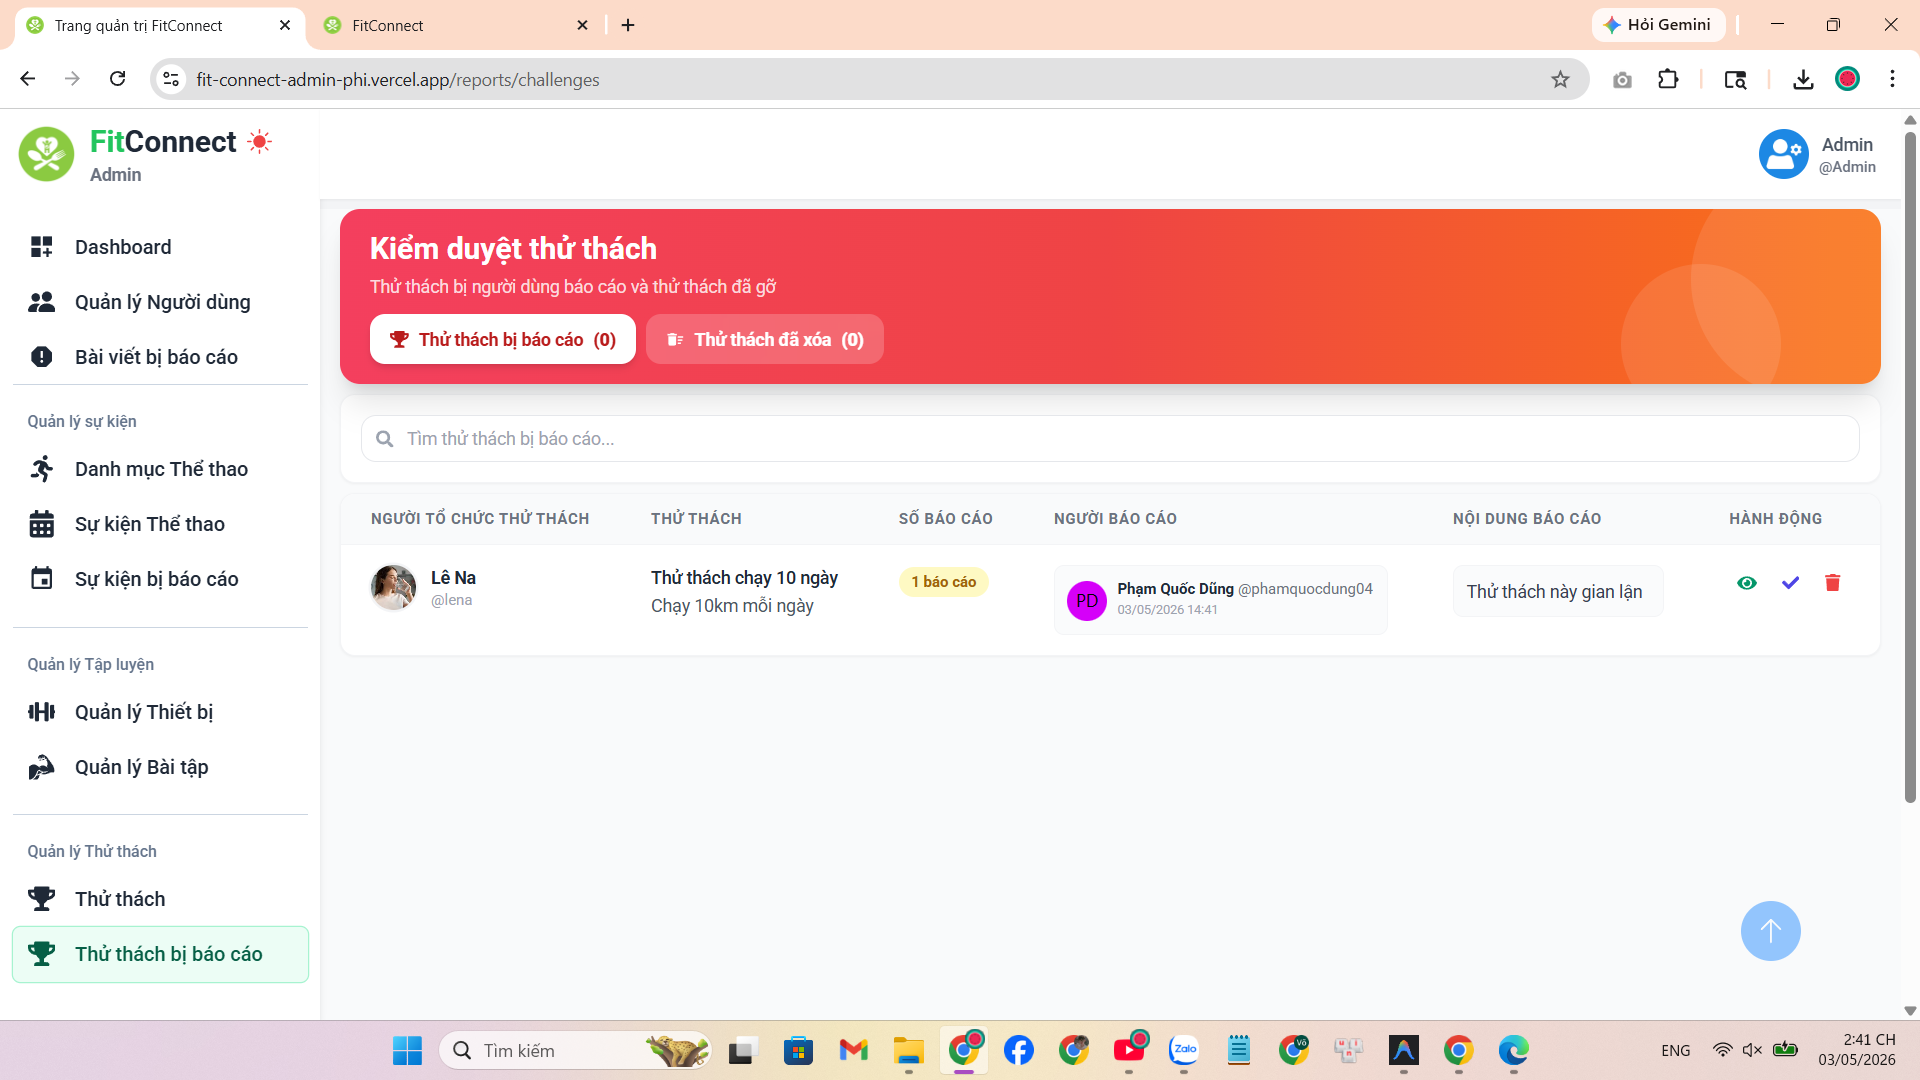
\includegraphics[width=0.60\textwidth]{Images/IMG/nhom9/kiemduyetthuthach/danhsachthuthachbibaocao.png}
    \caption{Quản trị viên theo dõi danh sách các thử thách bị người dùng báo cáo vi phạm}
    \label{fig:impl_admin_challenge_mod_reported_list}
\end{figure}


    \item Để đưa ra quyết định công bằng, Quản trị viên thực hiện xem chi tiết nội dung thử thách cùng với các lý do báo cáo cụ thể từ người dùng thông qua hộp thoại tích hợp.

\begin{figure}[H]
    \centering
    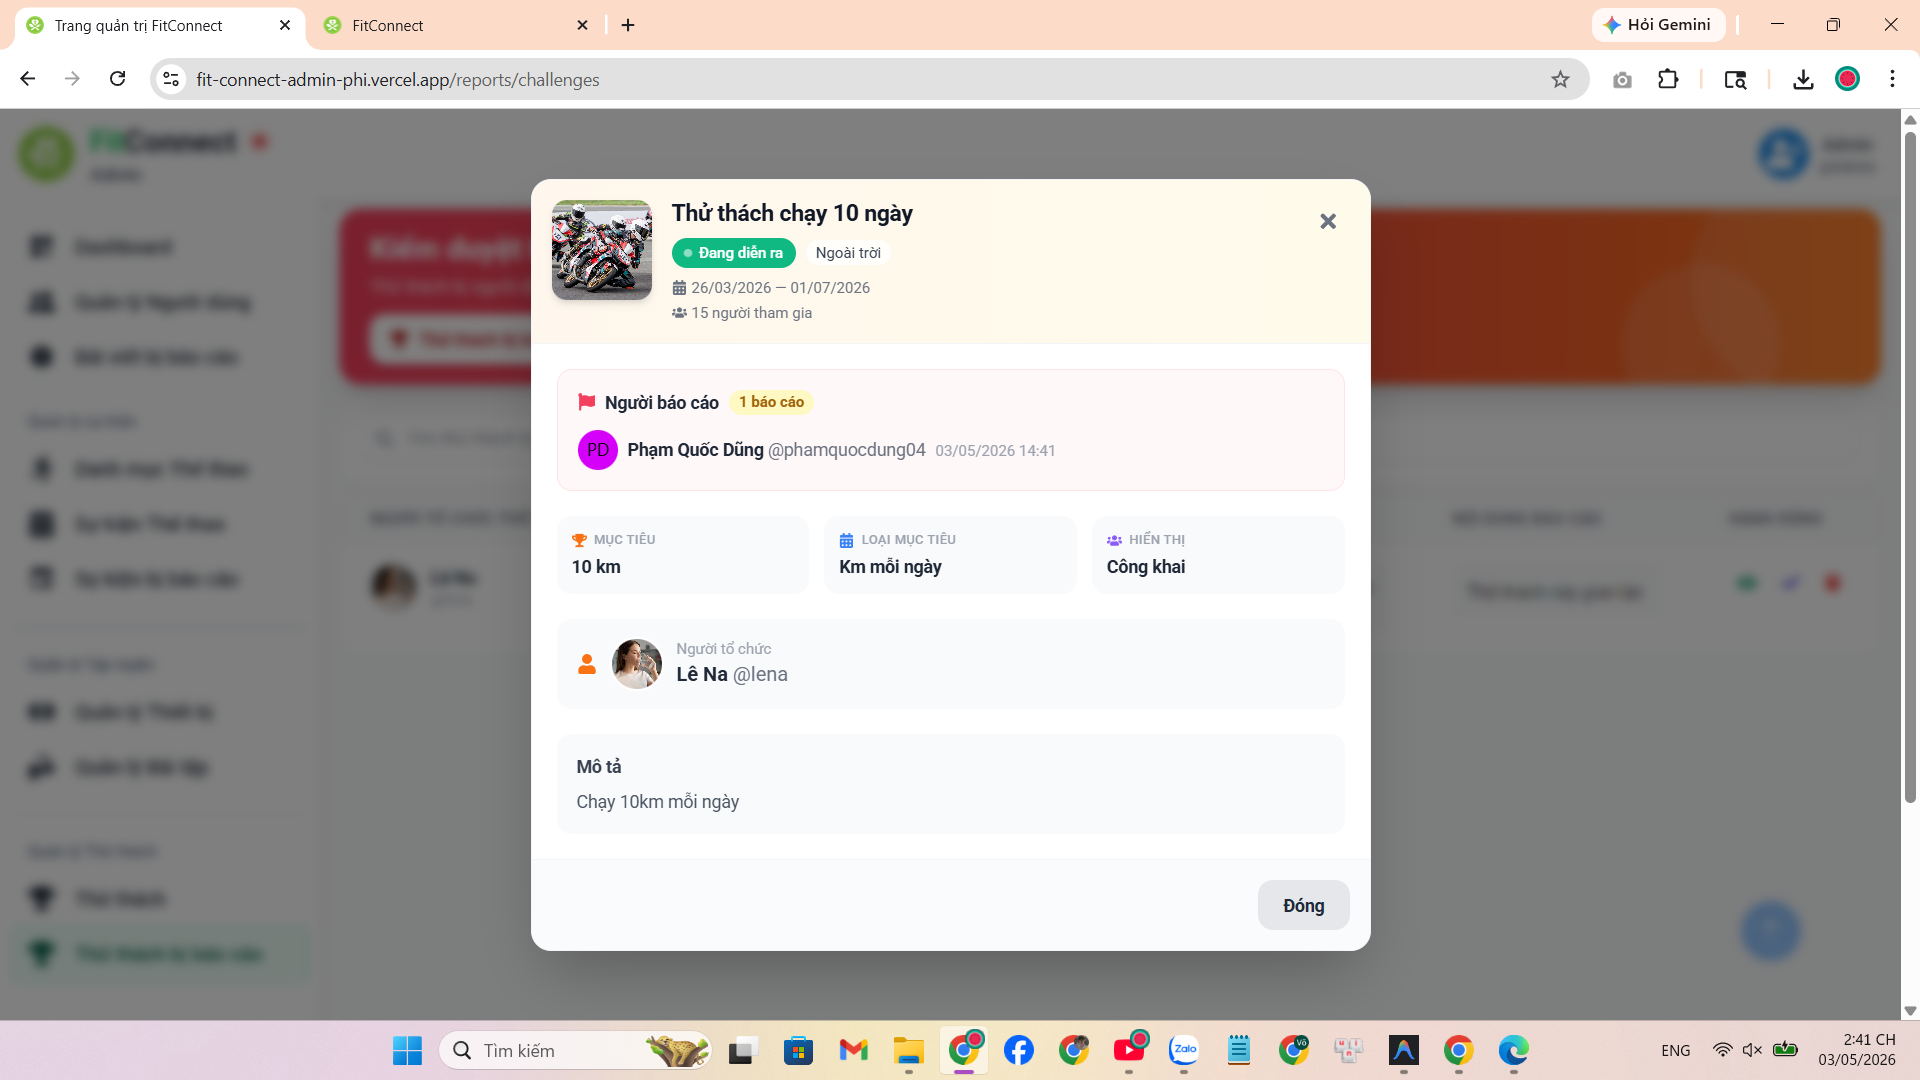
\includegraphics[width=0.60\textwidth]{Images/IMG/nhom9/kiemduyetthuthach/xemthongtinthuthach.png}
    \caption{Hệ thống hiển thị thông tin chi tiết thử thách và các báo cáo liên quan}
    \label{fig:impl_admin_challenge_mod_detail}
\end{figure}


    \item Dựa trên quá trình xác minh, Quản trị viên có hai hướng xử lý chính. Nếu nội dung báo cáo không chính xác, Admin chọn ``Giữ thử thách'' để bác bỏ các báo cáo và duy trì trạng thái hoạt động bình thường. Ngược lại, nếu vi phạm được xác nhận, Admin tiến hành gỡ bỏ thử thách.

\begin{figure}[H]
    \centering
    \begin{subfigure}[b]{0.47\textwidth}
        \centering
        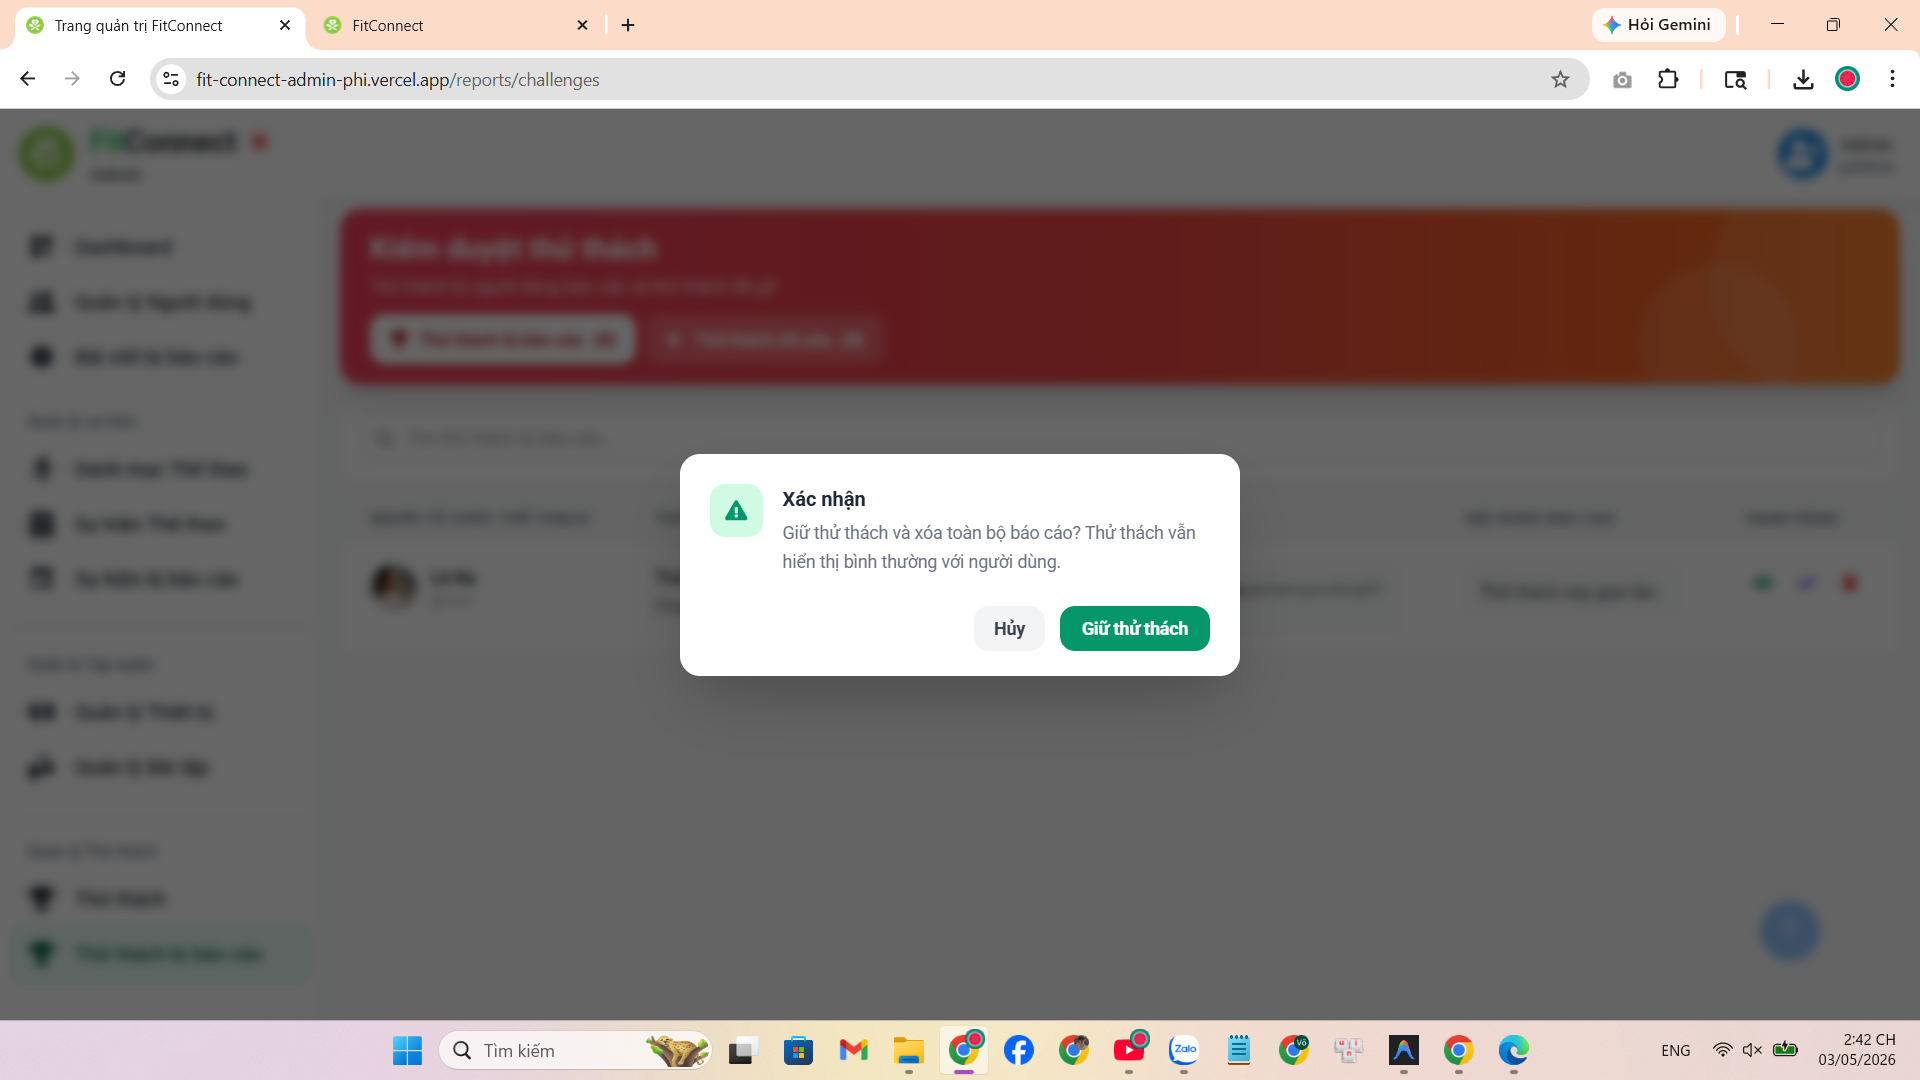
\includegraphics[width=\textwidth]{Images/IMG/nhom9/kiemduyetthuthach/giuthuthach.png}
        \caption{Hộp thoại xác nhận giữ lại thử thách khi báo cáo được xác định là không vi phạm}
        \label{fig:impl_admin_challenge_mod_keep}
    \end{subfigure}
    \hfill
    \begin{subfigure}[b]{0.47\textwidth}
        \centering
        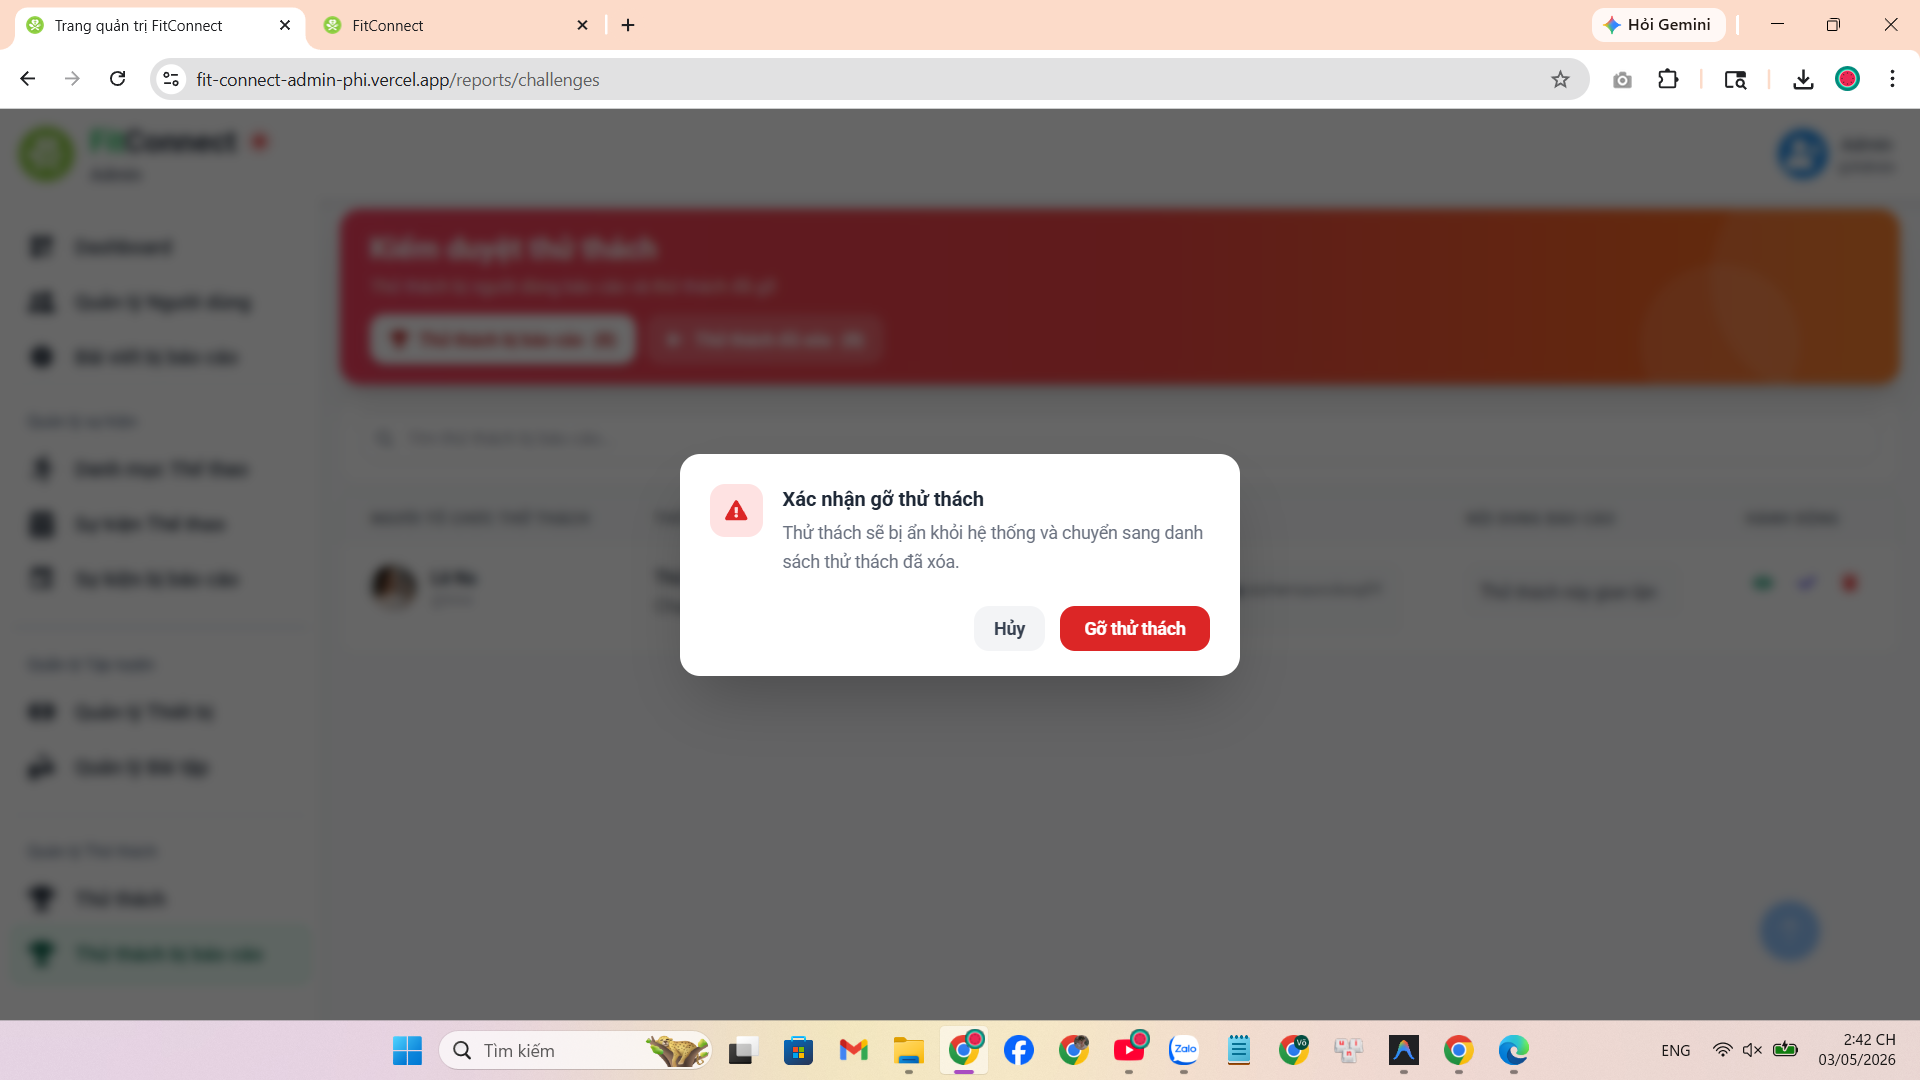
\includegraphics[width=\textwidth]{Images/IMG/nhom9/kiemduyetthuthach/xoathuthach.png}
        \caption{Hệ thống hiển thị hộp thoại xác nhận gỡ bỏ thử thách vi phạm tiêu chuẩn}
        \label{fig:impl_admin_challenge_mod_remove}
    \end{subfigure}
\end{figure}


    \item Thử thách bị gỡ bỏ chuyển sang chế độ chỉ đọc, người dùng không thể tham gia hay cập nhật kết quả mới. Toàn bộ thử thách đã gỡ được lưu tại tab ``Thử thách đã xóa'' và có thể khôi phục nếu cần.

\begin{figure}[H]
    \centering
    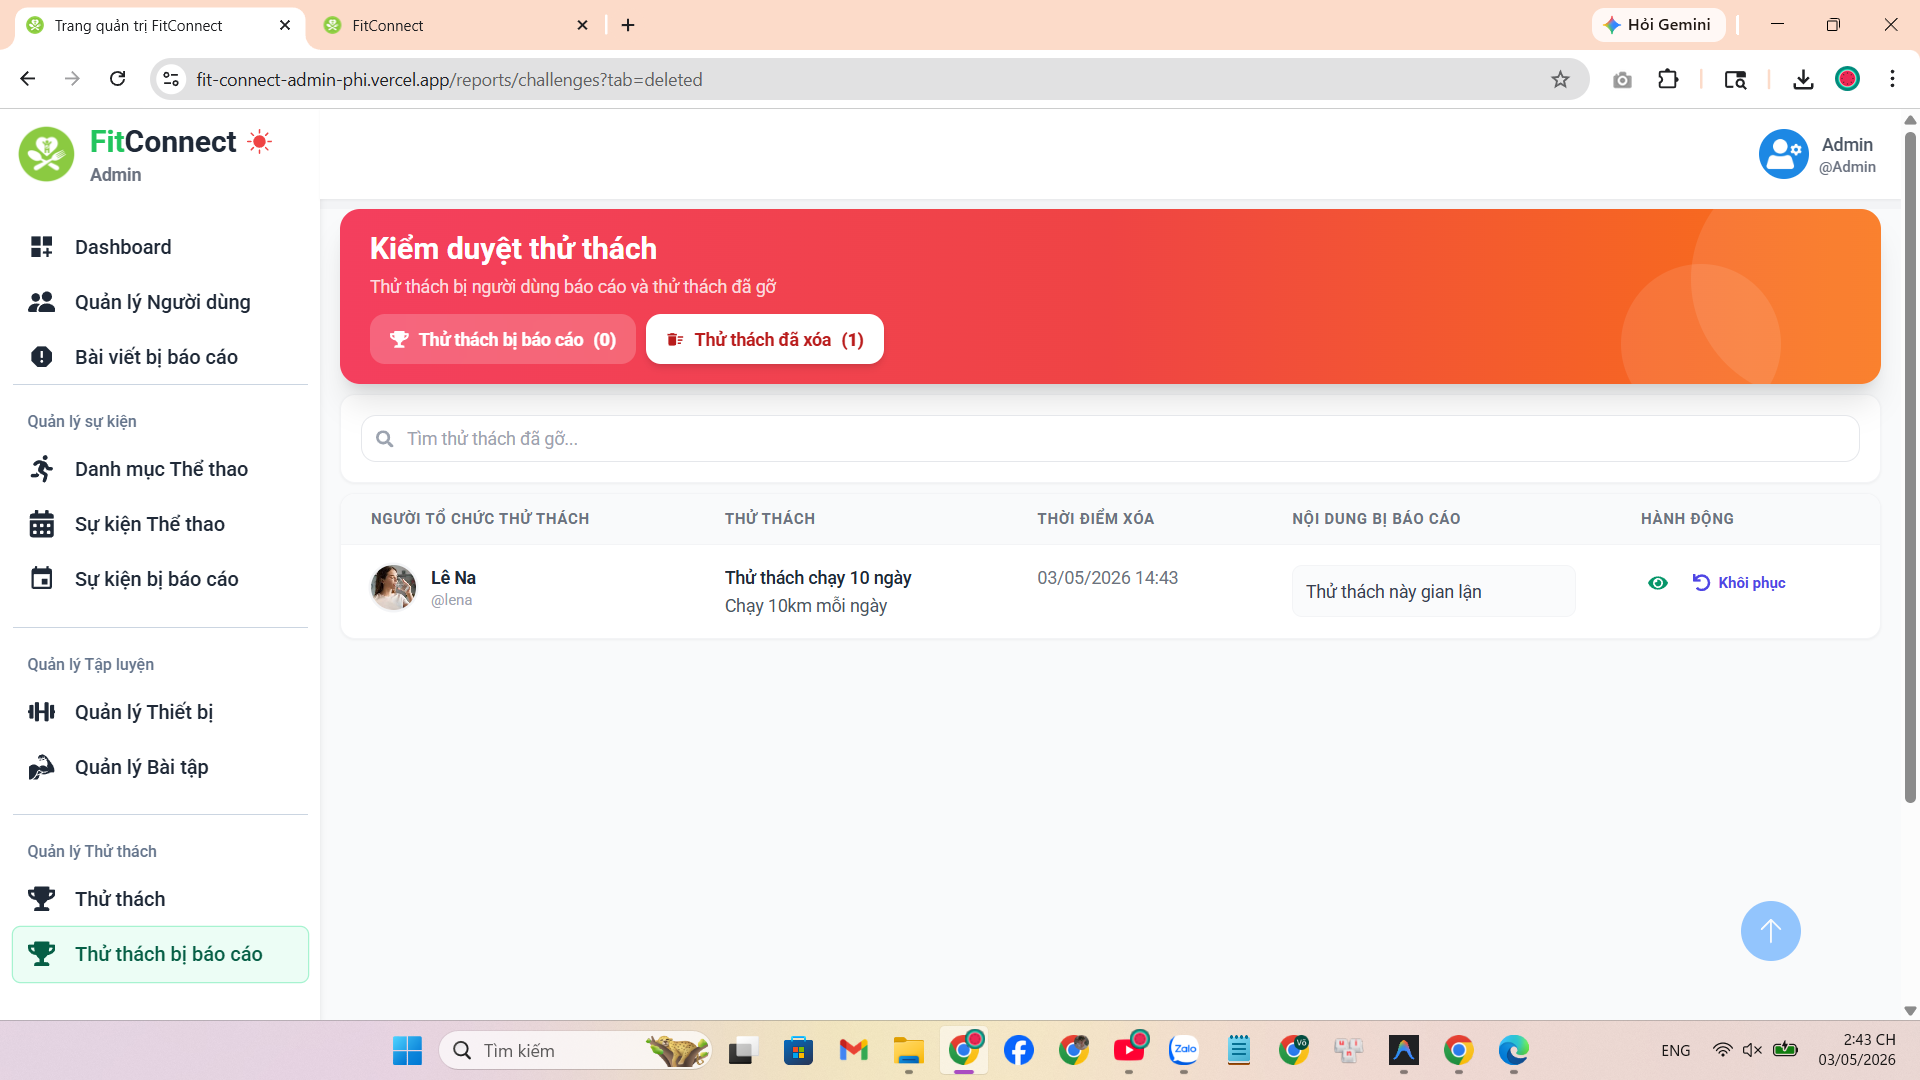
\includegraphics[width=0.60\textwidth]{Images/IMG/nhom9/kiemduyetthuthach/danhsachthuthachdaxoa.png}
    \caption{Danh sách thử thách đã bị gỡ bỏ do vi phạm, cho phép xem xét và khôi phục}
    \label{fig:impl_admin_challenge_mod_deleted_list}
\end{figure}

\end{itemize}

\section{Triển khai và vận hành}
\label{sec:impl_deployment}

Quy trình triển khai và vận hành đóng vai trò quyết định trong việc đưa hệ thống FitConnect từ môi trường phát triển sang môi trường thực tế, đảm bảo tính ổn định, bảo mật và khả năng mở rộng.

\subsection{Cơ sở hạ tầng và Môi trường triển khai}
\label{subsec:impl_infrastructure}

Hệ thống được triển khai trên \textbf{máy chủ VPS Ubuntu} theo sơ đồ Hình~\ref{fig:vps_deploy_diagram} (Chương~\ref{chap:technology}): một điểm vào duy nhất qua \textbf{HTTPS (443)} tới \textbf{Nginx}, vừa kết thúc SSL/TLS, vừa phục vụ file tĩnh và chuyển tiếp API/WebSocket tới tầng ứng dụng.

\begin{itemize}
    \item \textbf{Nginx:} Cấu hình phục vụ thư mục build của \textbf{DATN\_FE} và \textbf{DATN\_ADMIN\_FE} (artefact sau \texttt{npm run build} / Vite thường là \texttt{dist}); đồng thời \texttt{proxy\_pass} các đường dẫn \texttt{/api/...} và \texttt{/socket.io/...} tới tiến trình Node nội bộ.
    \item \textbf{Backend (DATN\_BE):} Chạy trực tiếp trên Node.js (ứng dụng \textbf{Express} tích hợp \textbf{Socket.IO}), được giữ tiến trình bằng \textbf{PM2} để tự khởi động lại khi lỗi và thuận tiện giám sát tài nguyên.
    \item \textbf{Cơ sở dữ liệu:} Có thể dùng \textbf{MongoDB cài trên cùng VPS} hoặc \textbf{MongoDB Atlas} (cloud); ứng dụng kết nối qua biến môi trường \texttt{MONGODB\_URL}.
    \item \textbf{Dịch vụ ngoài (không chạy trên VPS):} \textbf{Cloudinary} (media), \textbf{Goong Maps API} (bản đồ), \textbf{LLM API} (OpenAI-compatible / Groq, Gemini tùy cấu hình) --- Backend gọi ra Internet với khoá bí mật lưu phía server.
\end{itemize}

Việc đóng gói bằng \textbf{Docker} hoặc triển khai Frontend lên nền tảng edge (ví dụ Vercel) vẫn có thể áp dụng trong các biến thể khác, nhưng cấu hình chuẩn của đề tài là \textbf{tập trung trên một VPS} như trên để kiểm soát chi phí và phù hợp môi trường đồ án.

\subsection{Quy trình triển khai (Deployment Workflow)}
\label{subsec:impl_workflow}

Quy trình đưa phiên bản mới lên production trên VPS thường gồm các bước:
\begin{itemize}
    \item \textbf{Quản lý mã nguồn:} Dùng \textbf{Git} và \textbf{GitHub} để phiên bản hóa; trên máy chủ, \texttt{git pull} nhánh ổn định.
    \item \textbf{Build Frontend:} Trong thư mục \texttt{DATN\_FE} và \texttt{DATN\_ADMIN\_FE}, cài dependency (nếu cần), chạy \texttt{npm run build}, đồng bộ thư mục artefact tới đường dẫn mà Nginx đã cấu hình.
    \item \textbf{Build và khởi động Backend:} Trong \texttt{DATN\_BE}, cài dependency, biên dịch TypeScript (\texttt{npm run build} tùy script), khởi động lại bằng \texttt{pm2 restart} (hoặc \texttt{pm2 start} lần đầu).
    \item \textbf{Nginx:} Kiểm tra cú pháp (\texttt{nginx -t}) và \texttt{reload} khi đổi cấu hình server hoặc đường dẫn static.
    \item \textbf{CI/CD (tùy chọn):} Có thể tự động hóa các bước trên bằng GitHub Actions hoặc script SSH; không bắt buộc Docker Registry nếu chạy Node trực tiếp trên VPS.
\end{itemize}

\subsection{Giám sát, Bảo trì và Bảo mật}
\label{subsec:impl_monitoring}

\begin{table}[H]
\centering
\caption{Chiến lược giám sát và bảo mật hệ thống FitConnect}
\label{tab:impl_ops_security}
\small
\renewcommand{\arraystretch}{1.2}
\begin{tabular}{|p{3cm}|p{2.8cm}|p{8.2cm}|}
\hline
\textbf{Lĩnh vực} & \textbf{Công cụ / Cơ chế} & \textbf{Mô tả} \\
\hline
\textbf{Logging} & Winston + Morgan & Ghi nhật ký toàn bộ API request, response và lỗi hệ thống để truy vết sự cố. \\
\hline
\textbf{Monitoring} & PM2 Monit & Theo dõi CPU, RAM của Backend theo thời gian thực; tự động restart khi tiến trình crash. \\
\hline
\textbf{Mã hóa truyền tải} & HTTPS (SSL/TLS) & Toàn bộ dữ liệu giữa Client và Server được mã hóa end-to-end. \\
\hline
\textbf{Xác thực} & JWT + Google OAuth 2.0 & Access Token + Refresh Token đảm bảo phiên an toàn; OAuth 2.0 cho đăng nhập qua Google. \\
\hline
\textbf{Phân quyền} & Middleware checkRole & Tách biệt hoàn toàn route \texttt{/api/admin} khỏi route người dùng thông thường. \\
\hline
\textbf{Phòng thủ ứng dụng} & CORS + Rate Limiting + Bcrypt & Chỉ cho phép domain tin cậy; giới hạn 100 req/15 phút mỗi IP; băm mật khẩu một chiều. \\
\hline
\textbf{Sanitization} & Joi/Yup + DOMPurify & Validate schema đầu vào phía server; lọc XSS/NoSQL Injection trước khi xử lý. \\
\hline
\end{tabular}
\end{table}

\section{Kết luận chương}
\label{sec:impl_conclusion}

Chương 6 đã trình bày toàn bộ quá trình hiện thực hệ thống FitConnect: từ môi trường phát triển, 9 nhóm tính năng cốt lõi, tích hợp AI, đến triển khai và vận hành Production. Hệ thống đã hoàn thiện kiến trúc RESTful API (Node.js + Express), giao diện React với quản lý trạng thái React Query, triển khai trên \textbf{VPS} (Nginx, PM2, HTTPS) kết hợp MongoDB (cục bộ hoặc Atlas), Cloudinary và các API ngoài; bảo mật đa tầng gồm JWT, OAuth 2.0, HTTPS và Rate Limiting. Kết quả này là nền tảng để tiến hành kiểm thử toàn diện ở Chương 7.



\chapter{KIỂM THỬ HỆ THỐNG}
\renewcommand*{\theHsection}{\theHchapter.\the\value{section}}
Chương này trình bày quá trình kiểm thử toàn diện hệ thống FitConnect ở nhiều cấp độ: Unit, Integration, API, Functional, Hiệu năng, Bảo mật và Tương thích.

\section{Mục tiêu, Phạm vi và Phương pháp kiểm thử}
\label{sec:test_objectives}

Hệ thống FitConnect áp dụng mô hình \textbf{Kim tự tháp kiểm thử} (Testing Pyramid), nhấn mạnh nền tảng Unit Test vững chắc kết hợp Integration Test và Functional Test. Mục tiêu bao gồm: xác minh tính đúng đắn của logic nghiệp vụ (tính calo, GPS, gợi ý AI), đánh giá hiệu năng API và khả năng chịu tải, kiểm tra bảo mật phân quyền (JWT/OAuth), và đảm bảo tương thích đa thiết bị.

\begin{table}[H]
\centering
\caption{Phạm vi và công cụ kiểm thử hệ thống FitConnect}
\label{tab:test_scope}
\small
\renewcommand{\arraystretch}{1.2}
\begin{tabular}{|p{3.5cm}|p{3.5cm}|p{7cm}|}
\hline
\textbf{Loại kiểm thử} & \textbf{Công cụ} & \textbf{Phạm vi} \\
\hline
Unit \& Integration & Jest + React Testing Library & Hàm tính TDEE/BMI/GPS; component React độc lập \\
\hline
API Testing & Postman, Thunder Client & Toàn bộ REST endpoint (73 endpoints) \\
\hline
Functional (UAT) & Thủ công & 65 kịch bản theo 9 nhóm tính năng \\
\hline
Performance & Google PageSpeed, Loader.io & Thời gian tải trang, chịu tải 1.000 user đồng thời \\
\hline
Database & MongoDB Atlas Metrics & Opcounters, latency trên Replica Set 3 nodes \\
\hline
Security & Helmet, CORS Analyzer & JWT, phân quyền, Rate Limiting, XSS/Injection \\
\hline
Compatibility & Chrome DevTools & Desktop, Tablet, Mobile (375px+) \\
\hline
\end{tabular}
\end{table}

\section{Kiểm thử Unit}
\label{sec:test_unit}

\subsection{Backend Unit Tests}
Kiểm thử tập trung vào các hàm nghiệp vụ độc lập, ví dụ như logic tính toán lượng calo dựa trên chỉ số MET (Metabolic Equivalent of Task) hoặc xác thực Token.

\textbf{Ví dụ: Kiểm thử hàm tính toán lượng calo tiêu hao}


\subsection{Kết quả kiểm thử Unit}
\begin{table}[H]
    \centering
    \caption{Tổng hợp kết quả kiểm thử Unit}
    \begin{tabular}{|l|c|c|c|c|}
        \hline
        \textbf{Module} & \textbf{Tổng số Tests} & \textbf{Passed} & \textbf{Failed} & \textbf{Tỉ lệ bao phủ (Coverage)} \\
        \hline
        Auth Services & 15 & 15 & 0 & 95\% \\
        \hline
        Fitness Utilities & 20 & 20 & 0 & 100\% \\
        \hline
        AI Proxy Logic & 10 & 10 & 0 & 90\% \\
        \hline
        React Components & 35 & 33 & 2 & 82\% \\
        \hline
        \textbf{Tổng cộng} & \textbf{80} & \textbf{78} & \textbf{2} & \textbf{88.5\%} \\
        \hline
    \end{tabular}
\end{table}

\section{Kiểm thử Integration và API}
\label{sec:test_api}

\subsection{Kiểm thử với Postman}
Toàn bộ các endpoint API được hệ thống hóa thành Collection trên Postman, bao gồm các kịch bản kiểm tra: tính hợp lệ của Token, CRUD thao tác cho Bài viết (Posts), quản lý Sự kiện và Thử thách cộng đồng.

\subsection{Kết quả kiểm thử API}
\begin{table}[H]
    \centering
    \caption{Kết quả kiểm thử API Endpoints}
    \begin{tabular}{|l|c|c|c|}
        \hline
        \textbf{Nhóm API} & \textbf{Tổng số Endpoints} & \textbf{Passed} & \textbf{Failed} \\
        \hline
        Authentication \& Users & 12 & 12 & 0 \\
        \hline
        Community \& Posts & 15 & 14 & 1 \\
        \hline
        Sport Events \& Challenges & 18 & 18 & 0 \\
        \hline
        Workout \& AI Suggestion & 8 & 8 & 0 \\
        \hline
        Admin Management & 20 & 19 & 1 \\
        \hline
        \textbf{Tổng cộng} & \textbf{73} & \textbf{71} & \textbf{2} \\
        \hline
    \end{tabular}
\end{table}

\section{Kiểm thử chức năng}
\label{sec:test_functional}

\subsection{Tổng hợp kịch bản kiểm thử theo 9 nhóm tính năng}

Hệ thống FitConnect được kiểm thử chức năng theo toàn bộ 9 nhóm tính năng cốt lõi.
Bảng~\ref{tab:tc_summary} tổng hợp 15 kịch bản Happy Case đại diện.

\begin{table}[H]
    \centering
    \caption{Tổng hợp kịch bản kiểm thử chức năng theo 9 nhóm tính năng}
    \label{tab:tc_summary}
    \begin{tabular}{|c|p{4cm}|p{6.5cm}|c|}
        \hline
        \textbf{Mã} & \textbf{Nhóm tính năng} & \textbf{Kịch bản kiểm thử} & \textbf{Kết quả} \\
        \hline
        TC-01 & Tài khoản \& Hồ sơ & Đăng ký tài khoản mới & \checkmark Passed \\
        \hline
        TC-02 & Tài khoản \& Hồ sơ & Đăng nhập và nhận Access Token & \checkmark Passed \\
        \hline
        TC-03 & Tài khoản \& Hồ sơ & Khôi phục mật khẩu qua OTP Email & \checkmark Passed \\
        \hline
        TC-04 & Mạng xã hội cộng đồng & Đăng bài viết hợp lệ kèm hình ảnh & \checkmark Passed \\
        \hline
        TC-05 & Mạng xã hội cộng đồng & Thích và bình luận bài viết & \checkmark Passed \\
        \hline
        TC-06 & Sự kiện thể thao & Tham gia sự kiện thể thao ngoài trời & \checkmark Passed \\
        \hline
        TC-07 & Sự kiện thể thao & Ghi nhận hoạt động GPS trong sự kiện & \checkmark Passed \\
        \hline
        TC-08 & Thử thách cộng đồng & Tham gia thử thách và check-in tiến độ & \checkmark Passed \\
        \hline
        TC-09 & Thử thách cộng đồng & Admin vô hiệu hóa thử thách vi phạm & \checkmark Passed \\
        \hline
        TC-10 & Tính toán sức khỏe & Tính BMI và nhận phân tích AI & \checkmark Passed \\
        \hline
        TC-11 & Tập luyện & Tạo và hoàn thành buổi tập tùy chỉnh & \checkmark Passed \\
        \hline
        TC-12 & Tập luyện & AI gợi ý bài tập theo mô tả sức khỏe & \checkmark Passed \\
        \hline
        TC-13 & Lịch \& Thông báo & Xem sự kiện trên Lịch cá nhân & \checkmark Passed \\
        \hline
        TC-14 & Bạn bè & Gửi và chấp nhận lời mời kết bạn & \checkmark Passed \\
        \hline
        TC-15 & Quản trị hệ thống & Admin kiểm duyệt và gỡ bài viết vi phạm & \checkmark Passed \\
        \hline
    \end{tabular}
\end{table}

\subsection{Chi tiết kịch bản kiểm thử}

\subsubsection*{Nhóm 1 -- Quản lý Tài khoản \& Hồ sơ}

\textbf{TC-01: Đăng ký tài khoản mới thành công}
\begin{itemize}
    \item \textbf{Điều kiện tiên quyết:} Người dùng chưa có tài khoản, email chưa được đăng ký trong hệ thống.
    \item \textbf{Các bước:}
    \begin{enumerate}
        \item Truy cập trang Đăng ký (\texttt{/register}).
        \item Nhập đầy đủ: Họ tên, email hợp lệ, mật khẩu $\geq$ 8 ký tự, xác nhận mật khẩu.
        \item Nhấn nút \textbf{Đăng ký}.
    \end{enumerate}
    \item \textbf{Kết quả mong đợi:} Tài khoản được tạo, mật khẩu băm (bcrypt) lưu vào CSDL. Hệ thống thông báo thành công và chuyển về trang Đăng nhập.
    \item \textbf{Kết quả thực tế:} \checkmark Passed.
\end{itemize}

\textbf{TC-02: Đăng nhập thành công và nhận Access Token hợp lệ}
\begin{itemize}
    \item \textbf{Điều kiện tiên quyết:} Tài khoản đã được đăng ký.
    \item \textbf{Các bước:}
    \begin{enumerate}
        \item Truy cập trang Đăng nhập (\texttt{/login}).
        \item Nhập email và mật khẩu đúng, nhấn \textbf{Đăng nhập}.
    \end{enumerate}
    \item \textbf{Kết quả mong đợi:} Hệ thống cấp Access Token (JWT), lưu vào bộ nhớ cục bộ. Chuyển hướng về \texttt{/home}, hiển thị đúng thông tin người dùng.
    \item \textbf{Kết quả thực tế:} \checkmark Passed.
\end{itemize}

\textbf{TC-03: Khôi phục mật khẩu qua OTP Email}
\begin{itemize}
    \item \textbf{Điều kiện tiên quyết:} Tài khoản đã tồn tại và có email hợp lệ.
    \item \textbf{Các bước:}
    \begin{enumerate}
        \item Nhấn \textbf{Quên mật khẩu}, nhập email tài khoản.
        \item Mở hòm thư, sao chép mã OTP 6 chữ số.
        \item Nhập OTP vào giao diện xác thực, nhập mật khẩu mới và xác nhận.
        \item Nhấn \textbf{Đặt lại mật khẩu}.
    \end{enumerate}
    \item \textbf{Kết quả mong đợi:} Email OTP gửi trong vòng 30 giây. Sau khi xác thực OTP hợp lệ, mật khẩu được cập nhật; người dùng đăng nhập được bằng mật khẩu mới ngay lập tức.
    \item \textbf{Kết quả thực tế:} \checkmark Passed.
\end{itemize}

\subsubsection*{Nhóm 2 -- Mạng xã hội cộng đồng}

\textbf{TC-04: Đăng bài viết hợp lệ kèm hình ảnh}
\begin{itemize}
    \item \textbf{Điều kiện tiên quyết:} Người dùng đã đăng nhập.
    \item \textbf{Các bước:}
    \begin{enumerate}
        \item Truy cập trang Cộng đồng, nhấn \textbf{Tạo bài viết}.
        \item Nhập nội dung, đính kèm 1 hình ảnh không vi phạm, chọn chế độ Mọi người.
        \item Nhấn \textbf{Đăng bài}.
    \end{enumerate}
    \item \textbf{Kết quả mong đợi:} AI quét hình ảnh xác nhận an toàn. Bài viết xuất hiện ngay trên Bảng tin; người dùng nhận thông báo đăng bài thành công.
    \item \textbf{Kết quả thực tế:} \checkmark Passed.
\end{itemize}

\textbf{TC-05: Thích và bình luận bài viết người khác}
\begin{itemize}
    \item \textbf{Điều kiện tiên quyết:} Có bài viết trên Bảng tin; người dùng B đã đăng nhập.
    \item \textbf{Các bước:}
    \begin{enumerate}
        \item Trên Bảng tin, tìm bài viết của người khác, nhấn biểu tượng \textbf{Thích}.
        \item Nhập nội dung bình luận và nhấn \textbf{Gửi}.
    \end{enumerate}
    \item \textbf{Kết quả mong đợi:} Lượt thích tăng 1; bình luận hiển thị ngay theo thời gian thực. Chủ bài viết nhận thông báo có người thích và bình luận.
    \item \textbf{Kết quả thực tế:} \checkmark Passed.
\end{itemize}

\subsubsection*{Nhóm 3 -- Sự kiện thể thao}

\textbf{TC-06: Tham gia sự kiện thể thao ngoài trời}
\begin{itemize}
    \item \textbf{Điều kiện tiên quyết:} Người dùng đã đăng nhập; có sự kiện Ngoài trời đang mở đăng ký.
    \item \textbf{Các bước:}
    \begin{enumerate}
        \item Truy cập trang Sự kiện, lọc Ngoài trời, chọn sự kiện phù hợp.
        \item Xem chi tiết, nhấn \textbf{Tham gia} và xác nhận.
    \end{enumerate}
    \item \textbf{Kết quả mong đợi:} Nút chuyển thành Đã tham gia. Sự kiện xuất hiện trong tab Sự kiện trên trang cá nhân và trong Lịch cá nhân. Số người tham gia tăng thêm 1.
    \item \textbf{Kết quả thực tế:} \checkmark Passed.
\end{itemize}

\textbf{TC-07: Ghi nhận hoạt động GPS trong sự kiện ngoài trời}
\begin{itemize}
    \item \textbf{Điều kiện tiên quyết:} Đã tham gia sự kiện Ngoài trời đang diễn ra; trình duyệt cấp quyền vị trí GPS.
    \item \textbf{Các bước:}
    \begin{enumerate}
        \item Vào Chi tiết sự kiện, chọn ngày hoạt động, nhấn \textbf{Bắt đầu hoạt động}.
        \item Hệ thống hiển thị bản đồ và ghi lộ trình GPS theo thời gian thực.
        \item Nhấn \textbf{Kết thúc hoạt động} sau khi hoàn thành.
    \end{enumerate}
    \item \textbf{Kết quả mong đợi:} Lộ trình hiển thị trên bản đồ; khoảng cách (km) và calo tiêu hao được tính đúng. Tiến độ trong sự kiện cập nhật trên bảng xếp hạng.
    \item \textbf{Kết quả thực tế:} \checkmark Passed.
\end{itemize}

\subsubsection*{Nhóm 4 -- Thử thách cộng đồng}

\textbf{TC-08: Tham gia thử thách và check-in tiến độ hàng ngày}
\begin{itemize}
    \item \textbf{Điều kiện tiên quyết:} Người dùng đã đăng nhập; có thử thách đang mở tham gia.
    \item \textbf{Các bước:}
    \begin{enumerate}
        \item Truy cập trang Thử thách, chọn thử thách và nhấn \textbf{Tham gia}.
        \item Vào trang chi tiết, chọn ngày hôm nay, nhấn \textbf{Check-in}.
        \item Nhập dữ liệu tiến độ (số km, số phút hoặc tải ảnh bữa ăn), xác nhận.
    \end{enumerate}
    \item \textbf{Kết quả mong đợi:} Trạng thái ngày chuyển Đã check-in; streak (chuỗi ngày) tăng 1. Tiến độ cập nhật trên bảng xếp hạng thử thách.
    \item \textbf{Kết quả thực tế:} \checkmark Passed.
\end{itemize}

\textbf{TC-09: Admin vô hiệu hóa thử thách bị báo cáo vi phạm}
\begin{itemize}
    \item \textbf{Điều kiện tiên quyết:} Admin đăng nhập vào trang quản trị; có thử thách đã nhận báo cáo.
    \item \textbf{Các bước:}
    \begin{enumerate}
        \item Truy cập mục \textbf{Kiểm duyệt thử thách}, xem chi tiết thử thách bị báo cáo.
        \item Nhấn \textbf{Gỡ bỏ} và xác nhận.
    \end{enumerate}
    \item \textbf{Kết quả mong đợi:} Thử thách chuyển trạng thái Chỉ đọc -- người dùng không thể check-in mới. Hiển thị trong mục Thử thách đã xóa. Người tạo nhận thông báo vi phạm.
    \item \textbf{Kết quả thực tế:} \checkmark Passed.
\end{itemize}

\subsubsection*{Nhóm 5 -- Tính toán chỉ số sức khỏe}

\textbf{TC-10: Tính chỉ số BMI và nhận phân tích từ AI}
\begin{itemize}
    \item \textbf{Điều kiện tiên quyết:} Người dùng đã đăng nhập, truy cập trang Công cụ sức khỏe.
    \item \textbf{Các bước:}
    \begin{enumerate}
        \item Chọn công cụ \textbf{Tính chỉ số BMI}, nhập chiều cao và cân nặng, nhấn \textbf{Tính toán}.
        \item Nhấn \textbf{AI Phân Tích Sức Khỏe} để nhận đánh giá cá nhân hóa.
    \end{enumerate}
    \item \textbf{Kết quả mong đợi:} Kết quả BMI đúng (ví dụ: 22.5 -- Bình thường) với thang phân loại trực quan. AI trả về lời khuyên dinh dưỡng và bài tập gợi ý trong 5 giây. Kết quả lưu vào Lịch sử chỉ số sức khỏe.
    \item \textbf{Kết quả thực tế:} \checkmark Passed.
\end{itemize}

\subsubsection*{Nhóm 6 -- Tập luyện}

\textbf{TC-11: Tạo và hoàn thành buổi tập luyện tùy chỉnh}
\begin{itemize}
    \item \textbf{Điều kiện tiên quyết:} Người dùng đã đăng nhập, truy cập trang Tập luyện.
    \item \textbf{Các bước:}
    \begin{enumerate}
        \item Nhấn \textbf{Tạo buổi tập mới}, tìm kiếm và thêm 3 bài tập (Squat, Plank, Push-up).
        \item Nhập số set/reps từng bài, nhấn \textbf{Bắt đầu luyện tập}.
        \item Đánh dấu hoàn thành từng set, nhấn \textbf{Kết thúc buổi tập}.
    \end{enumerate}
    \item \textbf{Kết quả mong đợi:} Buổi tập lưu vào Lịch sử với tổng thời gian, số bài hoàn thành và kcal tiêu hao. Nhóm cơ kích hoạt hiển thị trực quan trên mô hình cơ thể người.
    \item \textbf{Kết quả thực tế:} \checkmark Passed.
\end{itemize}

\textbf{TC-12: AI gợi ý bài tập theo mô tả tình trạng sức khỏe}
\begin{itemize}
    \item \textbf{Điều kiện tiên quyết:} Người dùng đã đăng nhập.
    \item \textbf{Các bước:}
    \begin{enumerate}
        \item Truy cập \textbf{Lên kế hoạch tập luyện}, chọn tab \textbf{AI Gợi ý}.
        \item Nhập: ``Tôi muốn giảm mỡ bụng trong 30 phút, không đau lưng'', nhấn \textbf{Phân tích AI}.
        \item Chọn các bài tập từ danh sách gợi ý, nhấn \textbf{Bắt đầu luyện tập}.
    \end{enumerate}
    \item \textbf{Kết quả mong đợi:} Trong 3--5 giây, AI trả về đánh giá sức khỏe và danh sách bài phù hợp (Crunch, Plank, Mountain Climber) kèm lý do gợi ý. Người dùng sắp xếp thứ tự và bắt đầu tập được ngay.
    \item \textbf{Kết quả thực tế:} \checkmark Passed.
\end{itemize}

\subsubsection*{Nhóm 7 -- Lịch cá nhân \& Thông báo}

\textbf{TC-13: Xem sự kiện và thử thách trên Lịch cá nhân}
\begin{itemize}
    \item \textbf{Điều kiện tiên quyết:} Người dùng đang tham gia ít nhất một sự kiện và một thử thách.
    \item \textbf{Các bước:}
    \begin{enumerate}
        \item Truy cập trang \textbf{Lịch cá nhân}.
        \item Kiểm tra các ngày có sự kiện/thử thách; nhấn vào một mốc để xem chi tiết.
    \end{enumerate}
    \item \textbf{Kết quả mong đợi:} Lịch hiển thị đúng toàn bộ sự kiện và thử thách với màu phân loại. Nhấn vào ngày hiển thị đúng chi tiết và cho phép điều hướng tới trang tương ứng. Thông báo nhắc nhở xuất hiện đúng thời điểm sự kiện sắp diễn ra.
    \item \textbf{Kết quả thực tế:} \checkmark Passed.
\end{itemize}

\subsubsection*{Nhóm 8 -- Bạn bè}

\textbf{TC-14: Gửi lời mời kết bạn và được chấp nhận}
\begin{itemize}
    \item \textbf{Điều kiện tiên quyết:} Hai tài khoản User A và User B chưa kết bạn với nhau.
    \item \textbf{Các bước:}
    \begin{enumerate}
        \item User A truy cập trang cá nhân của User B, nhấn \textbf{Kết bạn}.
        \item User B nhận thông báo lời mời kết bạn, nhấn \textbf{Chấp nhận}.
    \end{enumerate}
    \item \textbf{Kết quả mong đợi:} User A và User B xuất hiện trong danh sách Bạn bè của nhau. Cả hai nhận thông báo kết bạn thành công theo thời gian thực. Bài viết của nhau xuất hiện trên Bảng tin tương ứng.
    \item \textbf{Kết quả thực tế:} \checkmark Passed.
\end{itemize}

\subsubsection*{Nhóm 9 -- Quản trị hệ thống}

\textbf{TC-15: Admin kiểm duyệt và gỡ bài viết vi phạm}
\begin{itemize}
    \item \textbf{Điều kiện tiên quyết:} Admin đã đăng nhập; có bài viết được người dùng báo cáo vi phạm.
    \item \textbf{Các bước:}
    \begin{enumerate}
        \item Truy cập \textbf{Admin Dashboard} $\rightarrow$ mục \textbf{Kiểm duyệt bài viết}.
        \item Xem nội dung bài viết bị báo cáo và lý do báo cáo.
        \item Nhấn \textbf{Xóa bài viết} và xác nhận tại popup.
    \end{enumerate}
    \item \textbf{Kết quả mong đợi:} Bài viết bị ẩn khỏi Bảng tin của tất cả người dùng và chuyển vào danh sách Bài viết đã xóa. Chủ bài viết nhận thông báo bài đã bị gỡ. Admin có thể khôi phục lại nếu cần.
    \item \textbf{Kết quả thực tế:} \checkmark Passed.
\end{itemize}

\subsection{Tổng hợp kết quả kiểm thử chức năng}
Hệ thống đã trải qua tổng cộng \textbf{65 kịch bản kiểm thử chức năng} (UAT -- User Acceptance Testing), trong đó \textbf{63 kịch bản thành công} (Tỉ lệ đạt: \textbf{96.9\%}). Bảng~\ref{tab:tc_summary} trình bày 15 kịch bản Happy Case tiêu biểu đại diện cho toàn bộ 9 nhóm tính năng, tất cả đều vượt qua. Các kịch bản lỗi còn lại chủ yếu liên quan đến độ trễ UI khi mạng yếu và đã được bổ sung Skeleton Loading để khắc phục.

\section{Kiểm thử hiệu năng và Trải nghiệm}
\label{sec:test_performance}

\subsection{Đo lường với Google PageSpeed Insights}
Để đảm bảo trải nghiệm người dùng mượt mà và tối ưu hóa công cụ tìm kiếm, giao diện Frontend được đánh giá bằng công cụ Google PageSpeed Insights trên phiên bản Desktop tại địa chỉ \url{https://fit-connect-tau.vercel.app/home}\footnote{\href{https://pagespeed.web.dev/analysis/https-fit-connect-tau-vercel-app-home/yl4fnfvyjw?form_factor=desktop}{Kết quả đo lường trực tiếp trên Google PageSpeed Insights}}:

\begin{figure}[H]
    \centering
    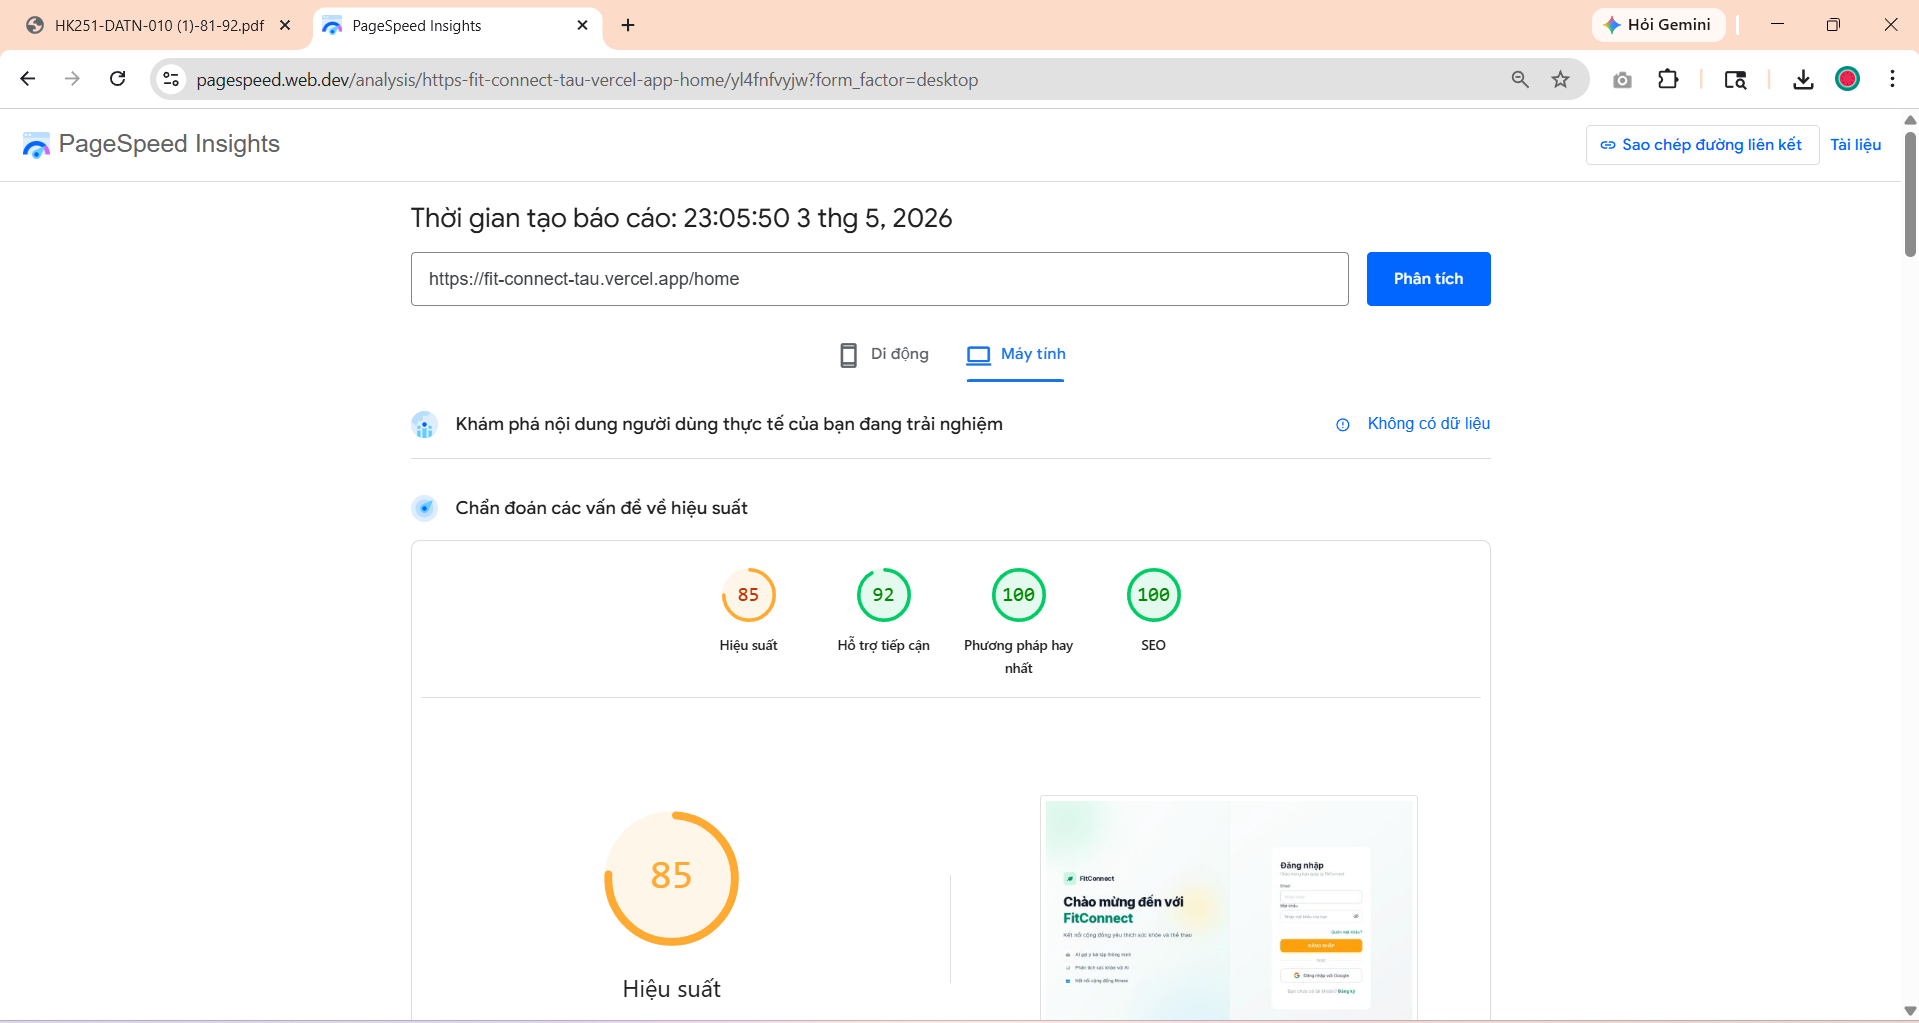
\includegraphics[width=\linewidth]{Images/IMG/test/PageSpeedInsights.png}
    \caption{Kết quả đánh giá chất lượng Frontend trên Google PageSpeed Insights (Desktop, ngày 03/05/2026)}
    \label{fig:pagespeed_test}
\end{figure}

\textbf{Phân tích kỹ thuật theo 4 tiêu chuẩn công nghiệp:}
\begin{itemize}
    \item \textbf{Hiệu suất (Performance - 85/100):} Điểm số ấn tượng đối với một ứng dụng SPA (Single Page Application) tích hợp nhiều thư viện nặng (MapBox, Chart.js, AI Models). Kết quả này chứng minh tính hiệu quả của chiến lược Code Splitting (chia nhỏ bundle) và tối ưu hóa tài nguyên hình ảnh qua Cloudinary CDN.
    \item \textbf{Khả năng tiếp cận (Accessibility - 92/100):} Đạt ngưỡng xuất sắc theo chuẩn WCAG. Hệ thống đảm bảo độ tương phản màu sắc tốt, cấu trúc cây DOM hợp lý và đầy đủ các thuộc tính ARIA, giúp người dùng khiếm khuyết có thể sử dụng dễ dàng qua các trình đọc màn hình.
    \item \textbf{Phương pháp tốt nhất (Best Practices - 100/100):} Điểm tuyệt đối chứng minh sự tuân thủ nghiêm ngặt các tiêu chuẩn bảo mật hiện đại: sử dụng HTTPS, ngăn chặn các lỗ hổng bảo mật trình duyệt phổ biến và tối ưu hóa tài nguyên mã nguồn.
    \item \textbf{SEO (100/100):} Khẳng định khả năng hiển thị tốt trên các công cụ tìm kiếm nhờ việc áp dụng kỹ thuật Semantic HTML5, quản lý thẻ Meta linh hoạt và cấu trúc dữ liệu thân thiện với AI Search.
\end{itemize}

\textbf{Nhận xét chung:} Điểm số cao trên cả 4 hạng mục là minh chứng cho việc hệ thống không chỉ chú trọng vào tính năng mà còn đạt được sự cân bằng tối ưu giữa hiệu năng và trải nghiệm người dùng cuối theo các tiêu chuẩn kỹ thuật web 2026.

\subsection{Kiểm thử tải với Loader.io}
Để đánh giá khả năng chịu tải và giới hạn xử lý của hệ thống, nhóm thực hiện mô phỏng áp lực với \textbf{1.000 người dùng đồng thời} truy cập trong vòng \textbf{1 phút} thông qua nền tảng Loader.io\footnote{\href{https://loader.io/tests/9df704ba8f2da90c2c3974753d26ed46}{Kết quả kiểm thử tải trực tuyến trên Loader.io}}:

\begin{figure}[H]
    \centering
    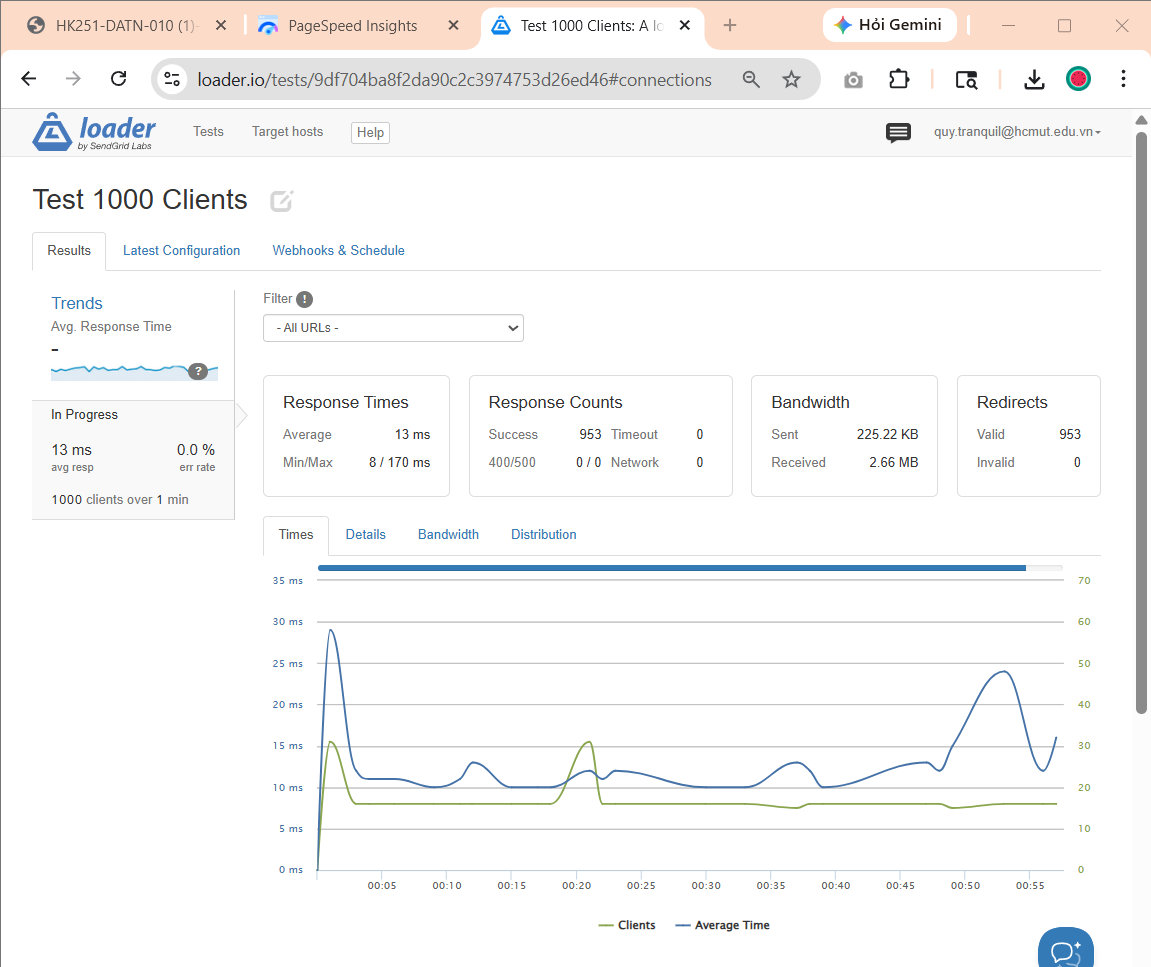
\includegraphics[width=\linewidth]{Images/IMG/test/loaderio.png}
    \caption{Kết quả kiểm thử tải với Loader.io -- 1.000 clients đồng thời trong 1 phút}
    \label{fig:loaderio_test}
\end{figure}

\textbf{Phân tích định lượng và chứng minh khả năng chịu tải:}
\begin{itemize}
    \item \textbf{Tốc độ phản hồi vượt trội:} Thời gian phản hồi trung bình chỉ \textbf{13ms}, thấp hơn rất nhiều so với ngưỡng tiêu chuẩn 200ms của Google. Điều này chứng minh kiến trúc Event Loop của Node.js hoạt động cực kỳ hiệu quả, không bị nghẽn (blocking) khi xử lý lượng lớn kết nối đồng thời.
    \item \textbf{Tính ổn định cao:} Khoảng cách giữa thời gian Min (8ms) và Max (170ms) là rất nhỏ, cho thấy không có hiện tượng rò rỉ bộ nhớ (Memory Leak) hay cạn kiệt tài nguyên hệ thống dưới áp lực cao. Hệ thống duy trì sự ổn định xuyên suốt chu kỳ kiểm thử.
    \item \textbf{Độ tin cậy tuyệt đối:} Tỉ lệ lỗi **0.0%** với **953/953 yêu cầu thành công** cho thấy hệ thống có khả năng xử lý lỗi ngoại lệ tốt và cấu hình máy chủ (Load Balancer, Web Server) đạt độ tối ưu cao.
    \item \textbf{Hiệu quả truyền tải dữ liệu:} Việc xử lý 2.66 MB dữ liệu trong 1 phút với 1.000 người dùng chứng minh cơ chế nén dữ liệu và truyền tải payload đã được cấu hình hợp lý, giúp tiết kiệm băng thông mà vẫn đảm bảo tốc độ.
\end{itemize}

\textbf{Nhận xét chung:} Kết quả từ Loader.io khẳng định nền tảng FitConnect không chỉ nhanh ở phía giao diện mà còn sở hữu một hạ tầng Backend vô cùng mạnh mẽ, đủ sức đáp ứng nhu cầu sử dụng thực tế của hàng nghìn người dùng cùng lúc mà không làm suy giảm chất lượng dịch vụ.

\subsection{Đo lường hiệu năng Cơ sở dữ liệu (Database Performance)}
Để đánh giá khả năng xử lý truy vấn thực tế, hệ thống sử dụng công cụ giám sát Metrics của MongoDB Atlas. Kết quả ghi nhận lượng thao tác (Opcounters) trên cụm cơ sở dữ liệu (Cluster) trong khoảng thời gian giám sát 2 tháng:

\begin{figure}[H]
    \centering
    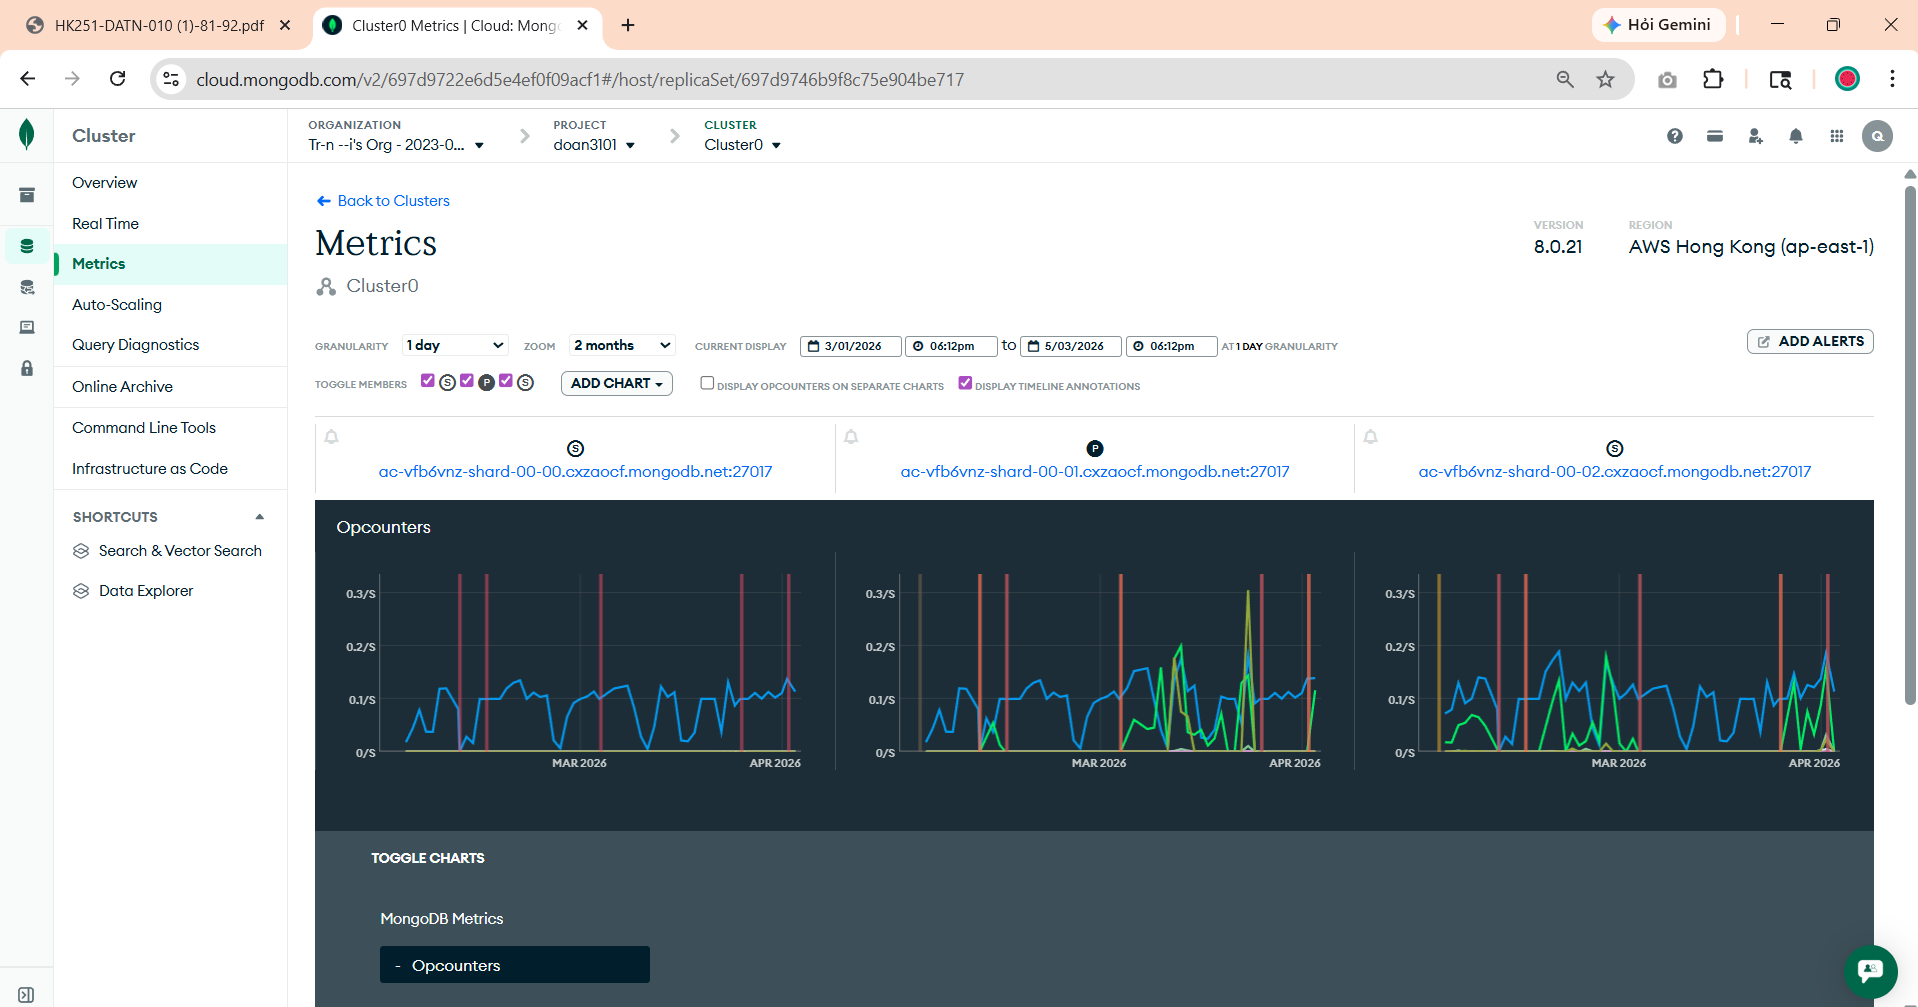
\includegraphics[width=\linewidth]{Images/IMG/test/OpcountersTest.png}
    \caption{Biểu đồ Opcounters trên cụm MongoDB Atlas (Replica Set 3 nodes)}
    \label{fig:mongodb_opcounters}
\end{figure}

\textbf{Phân tích định lượng và chứng minh kỹ thuật:}
\begin{itemize}
    \item \textbf{Hiệu suất xử lý (Throughput):} Biểu đồ ghi nhận tần suất thao tác trung bình dao động từ \textbf{0.1/s đến 0.3/s} (tương đương khoảng 8.600 - 25.000 thao tác mỗi ngày). Các chỉ số này duy trì ở biên độ hẹp, cho thấy hệ thống xử lý các yêu cầu truy xuất dữ liệu một cách mượt mà, không xảy ra hiện tượng trễ (latency) do nghẽn hàng đợi truy vấn.
    \item \textbf{Khả năng mở rộng đọc (Read Scalability):} Đường màu xanh lam (Queries) xuất hiện đồng nhất trên cả 3 nodes (Primary và 2 Secondaries). Điều này chứng minh cấu hình Read Preference đã hoạt động chính xác, cho phép phân tán tải trọng đọc ra các nút phụ, giúp giảm áp lực cho nút chính và tối ưu hóa thời gian phản hồi cho người dùng cuối.
    \item \textbf{Tính nhất quán dữ liệu (Data Consistency):} Các thao tác ghi (đường màu xanh lá - Updates/Commands) tập trung chủ yếu tại nút Primary (khung giữa). Điều này khẳng định cơ chế Single-Master Replication của hệ thống đang vận hành đúng thiết kế: mọi thay đổi dữ liệu được kiểm soát tập trung tại nút chính trước khi nhân bản, đảm bảo tính toàn vẹn và nhất quán của dữ liệu sức khỏe người dùng.
    \item \textbf{Độ tin cậy hệ thống (Uptime):} Dữ liệu trải dài liên tục trong 2 tháng (tháng 3 đến tháng 4 năm 2026) mà không có bất kỳ khoảng trống hay điểm rơi về 0 nào. Điều này là minh chứng thực tế cho khả năng vận hành bền bỉ và tính sẵn sàng cao (High Availability) của hạ tầng lưu trữ FitConnect.
\end{itemize}

Bên cạnh đó, nhờ việc thiết lập các bộ chỉ mục (Indexes) hợp lý, thời gian phản hồi thực tế của các truy vấn dữ liệu luôn được tối ưu ở mức thấp:
\begin{itemize}
    \item Truy vấn danh sách bài viết trên Bảng tin (có kết hợp phân trang): \textbf{$\sim$80ms}.
    \item Truy vấn tổng hợp tiến độ Thử thách cộng đồng (sử dụng Pipeline Aggregation phức tạp): \textbf{$\sim$150ms}.
    \item Tìm kiếm danh sách Bài tập thể dục (áp dụng Text Indexing): \textbf{$\sim$45ms}.
\end{itemize}

\section{Kiểm thử bảo mật}
\label{sec:test_security}

Các kịch bản kiểm thử bảo mật đã được thực hiện và vượt qua:
\begin{itemize}
    \item \textbf{Bảo mật Token:} Từ chối quyền truy cập khi sử dụng Token hết hạn hoặc bị chỉnh sửa trái phép (Mã lỗi 401 Unauthorized).
    \item \textbf{Input Validation:} Ngăn chặn thành công các luồng dữ liệu độc hại (XSS, NoSQL Injection) nhờ thư viện kiểm soát đầu vào (Joi, DOMPurify).
    \item \textbf{Phân quyền phân đoạn:} Xác nhận tài khoản User thông thường không thể truy cập các route bắt đầu bằng \texttt{/api/admin}.
    \item \textbf{Rate Limiting:} Kích hoạt chặn truy cập tạm thời khi một IP gửi quá 100 requests / 15 phút vào endpoint đăng nhập.
\end{itemize}

\section{Kiểm thử tương thích}
\label{sec:test_compatibility}

Hệ thống được thiết kế theo nguyên tắc Mobile-First và sử dụng Tailwind CSS, đảm bảo tính tương thích cao:
\begin{itemize}
    \item \textbf{Trình duyệt:} Hoạt động ổn định trên Google Chrome (v110+), Firefox (v100+), Safari (v15+) và Microsoft Edge.
    \item \textbf{Thiết bị:} Giao diện co giãn mượt mà trên Desktop (1920x1080), Tablet (iPad 768x1024), và thiết bị di động (iPhone/Android màn hình nhỏ từ 375px). Giao diện Admin Dashboard được ưu tiên sử dụng trên Tablet và Desktop để đảm bảo không gian hiển thị biểu đồ.
\end{itemize}

\section{Phát hiện và Xử lý lỗi}
\label{sec:test_bug_tracking}

Trong quá trình kiểm thử, một số lỗi thực tế đã được phát hiện và xử lý kịp thời:
\begin{itemize}
    \item \textbf{Lỗi đồng bộ dữ liệu sau khi sửa sự kiện (Bug-01):} Dữ liệu sự kiện trên UI không cập nhật ngay sau khi Admin chỉnh sửa. \textbf{Giải pháp:} Thiết lập \texttt{invalidateQueries} của React Query và tùy chỉnh \texttt{staleTime} về 1 giây cho các danh sách quan trọng.
    \item \textbf{Lỗi không đồng bộ loại sự kiện (Bug-02):} Xung đột do dữ liệu cũ lưu "Indoor" nhưng Frontend hiển thị "Trong nhà". \textbf{Giải pháp:} Thực hiện Database Migration để chuẩn hóa dữ liệu sang dạng phân loại ID/Enum chuẩn của hệ thống.
\end{itemize}

\section{Kết luận}
\label{sec:test_conclusion}

Sau quá trình kiểm thử toàn diện từ mức đơn vị (Unit) đến toàn hệ thống (bao gồm kiểm thử tải thực tế), FitConnect đã chứng minh được tính ổn định và sự hoàn thiện của các chức năng nghiệp vụ.
\begin{itemize}
    \item \textbf{Tỉ lệ kiểm thử thành công tổng thể (Pass rate)} đạt trên 96\%.
    \item \textbf{Các lỗi nghiêm trọng (Critical/High bugs)} đều đã được phát hiện và khắc phục kịp thời.
    \item \textbf{Kiểm thử tải (Loader.io):} Hệ thống xử lý thành công 1.000 người dùng đồng thời với thời gian phản hồi trung bình 13ms và tỉ lệ lỗi 0\%, đáp ứng tốt yêu cầu về khả năng chịu tải.
    \item \textbf{Chất lượng Frontend (PageSpeed Insights):} Đạt điểm SEO và Best Practices tuyệt đối 100/100; hiệu suất 85/100 và khả năng tiếp cận 92/100 -- đảm bảo trải nghiệm người dùng chất lượng cao.
    \item \textbf{Hiệu năng Cơ sở dữ liệu (MongoDB Atlas):} Cụm Replica Set hoạt động ổn định, phân tán tải trọng đọc/ghi mượt mà, thời gian đáp ứng các truy vấn phức tạp (Aggregation) luôn duy trì ở mức tối ưu (dưới 150ms) nhờ kỹ thuật đánh chỉ mục hợp lý.
    \item Hệ thống đảm bảo chặt chẽ các chỉ tiêu về bảo mật, tính sẵn sàng cao (High Availability) và tương thích tốt trên đa nền tảng.
\end{itemize}
Với các kết quả khả quan này, hệ thống FitConnect được đánh giá là đủ điều kiện an toàn và chất lượng để chính thức đưa vào triển khai và phục vụ người dùng cuối.


% \chapter{GIAO DIỆN HIỆN THỰC}
% \renewcommand*{\theHsection}{\theHchapter.\the\value{section}}
% \input{ui}

% \chapter{MÃ NGUỒN}
% \renewcommand*{\theHsection}{\theHchapter.\the\value{section}}
% \input{source-code}

\chapter{TỔNG KẾT}
\renewcommand*{\theHsection}{\theHchapter.\the\value{section}}
% !TeX root = main.tex

Dự án ``Xây dựng nền tảng mạng xã hội rèn luyện thể dục thể thao cộng đồng FitConnect'' đã được hoàn thành với kết quả vượt ngoài mong đợi ban đầu. Nhìn lại toàn bộ hành trình từ ý tưởng đến sản phẩm hoàn chỉnh, đây là một nỗ lực nghiêm túc và có tính tiên phong nhằm lấp đầy khoảng trống mà các nền tảng hiện tại chưa giải quyết được: tích hợp sâu giữa mạng xã hội cộng đồng và các công cụ hỗ trợ rèn luyện sức khỏe cá nhân trong một hệ sinh thái duy nhất, được dẫn dắt bởi Trí tuệ nhân tạo.

\section{Kết quả đạt được}

\subsection{Hiện thực đầy đủ 9 nhóm tính năng cốt lõi}

Hệ thống FitConnect đã được hiện thực thành công toàn bộ 9 nhóm tính năng cốt lõi đã đề ra trong giai đoạn phân tích yêu cầu, mỗi nhóm đều được triển khai đến mức độ sẵn sàng đưa vào sử dụng thực tế.

\textbf{Nhóm 1 -- Quản lý tài khoản và hồ sơ người dùng:} Hệ thống cung cấp đầy đủ quy trình đăng ký, đăng nhập thông qua email lẫn Google OAuth 2.0, cơ chế khôi phục mật khẩu an toàn bằng mã OTP 6 chữ số gửi qua email, và một không gian Profile Dashboard toàn diện cho phép người dùng cá nhân hóa hồ sơ (ảnh đại diện, ảnh nền, thông tin cá nhân, thông số nhân trắc học) đồng thời theo dõi lịch sử toàn bộ hoạt động bao gồm bài viết, sự kiện, thử thách và giáo án tập luyện.

\textbf{Nhóm 2 -- Mạng xã hội cộng đồng:} Bảng tin cộng đồng (Newsfeed) được xây dựng với đầy đủ tính năng của một mạng xã hội hiện đại: đăng bài viết kèm hình ảnh, bày tỏ cảm xúc, bình luận và trả lời bình luận theo luồng, chia sẻ nội dung. Điểm đặc biệt của nhóm tính năng này là sự tích hợp của hai lớp kiểm duyệt nội dung thông minh: mô hình NSFW Detection (TensorFlow.js) chạy trên trình duyệt để phát hiện hình ảnh nhạy cảm trước khi đăng, và bộ lọc từ ngữ tự động để chặn nội dung vi phạm tiêu chuẩn cộng đồng ngay cả trong phần bình luận. Cơ chế báo cáo vi phạm cộng đồng kết hợp với bảng điều khiển kiểm duyệt toàn diện của Quản trị viên tạo nên một vòng kiểm soát chặt chẽ.

\textbf{Nhóm 3 -- Sự kiện thể thao:} Đây là nhóm tính năng phức tạp và đặc trưng nhất của nền tảng. Hệ thống hỗ trợ song song hai hình thức thi đua: Ngoài trời (chạy bộ, đạp xe, leo núi) với tính năng theo dõi lộ trình GPS thời gian thực trên bản đồ Goong Maps, tự động tính toán quãng đường, tốc độ và calo tiêu hao; và Trong nhà (Yoga, Cardio, Gym) với không gian Video Call nhóm tích hợp AI nhận diện khuôn mặt (face-api.js) để tự động giám sát thời gian hiện diện hợp lệ của từng người tham gia, đảm bảo tính công bằng tuyệt đối. Ngoài ra, tính năng AI điền tự động thông tin sự kiện từ một đoạn mô tả ngôn ngữ tự nhiên đã rút ngắn đáng kể thời gian tổ chức.

\textbf{Nhóm 4 -- Thử thách cộng đồng:} Ba loại hình thử thách (Ăn uống/Dinh dưỡng, Thể dục, Ngoài trời) đều được hiện thực với cơ chế check-in tiến độ chuyên biệt. Thử thách dinh dưỡng xác minh ảnh bữa ăn bằng AI đa phương thức; thử thách vận động tích hợp trực tiếp vào không gian tập luyện của nhóm tính năng 6; thử thách ngoài trời sử dụng lại cơ sở hạ tầng GPS đã xây dựng. Hệ thống lịch biểu trực quan giúp theo dõi chuỗi streak liên tục và bảng xếp hạng cộng đồng thời gian thực.

\textbf{Nhóm 5 -- Kết nối mạng lưới bạn bè:} Hệ thống xây dựng cơ chế kết bạn và theo dõi đầy đủ, với bảng tin (News Feed) ưu tiên hiển thị nội dung từ những người trong mạng lưới. Mọi hoạt động thể thao nổi bật như tham gia sự kiện hay chinh phục thử thách đều tự động cập nhật lên bảng tin để lan tỏa động lực trong cộng đồng.

\textbf{Nhóm 6 -- Tập luyện cá nhân:} Hệ thống tập luyện cá nhân cung cấp ba phương thức lựa chọn bài tập bổ sung lẫn nhau: tùy chỉnh thủ công theo thiết bị sẵn có hoặc nhóm cơ mục tiêu (với trực quan hóa nhóm cơ bắp qua thư viện React Body Highlighter), gợi ý AI thông minh dựa trên mô tả tình trạng sức khỏe bằng ngôn ngữ tự nhiên, hoặc sử dụng lại các giáo án đã lưu. Người dùng có thể lên lịch tập luyện hàng tuần và được nhắc nhở tự động, đồng thời tất cả buổi tập được lưu vào lịch sử chi tiết với calo tiêu hao, thời lượng và nhóm cơ đã kích hoạt. Tính năng theo dõi hoạt động thể thao ngoài trời độc lập (chạy bộ, đạp xe) cũng được tích hợp để chuẩn bị cho các sự kiện và thử thách.

\textbf{Nhóm 7 -- Tính toán các chỉ số sức khỏe và gợi ý AI:} Bộ công cụ tính toán y khoa bao gồm 8 chỉ số: BMI, BMR, TDEE, Body Fat, IBW (Cân nặng lý tưởng), LBM (Khối lượng cơ thể nạc), Calo đốt cháy và Lượng nước cần mỗi ngày. Mỗi lần tính toán đều được lưu vào lịch sử và hiển thị qua biểu đồ xu hướng theo thời gian. Đặc biệt, tính năng AI Phân Tích Sức Khỏe tổng hợp toàn bộ chỉ số để đưa ra lời khuyên dinh dưỡng và danh sách bài tập gợi ý cá nhân hóa từ kho dữ liệu của hệ thống.

\textbf{Nhóm 8 -- Lịch trình cá nhân và thông báo:} Giao diện Lịch cá nhân (Calendar) tự động đồng bộ tất cả hoạt động mà người dùng đã đăng ký -- sự kiện thể thao, thử thách cộng đồng, lịch tập luyện cá nhân -- vào một giao diện thống nhất. Hệ thống thông báo thời gian thực (Socket.io) gửi cảnh báo khi đến giờ tập, khi bạn bè tương tác và khi có mục tiêu sắp đến hạn.

\textbf{Nhóm 9 -- Quản trị hệ thống toàn diện:} Bảng điều khiển Quản trị viên (Admin Dashboard) tích hợp biểu đồ thống kê thời gian thực về tăng trưởng người dùng, mức độ tương tác theo từng nhóm tính năng và thống kê sử dụng AI theo danh mục. Quản trị viên có toàn quyền kiểm duyệt và xử lý mọi nội dung vi phạm (bài viết, sự kiện, thử thách, tài khoản) thông qua luồng báo cáo từ cộng đồng, đồng thời quản lý toàn bộ tài nguyên dữ liệu nền tảng bao gồm danh mục thể thao, thiết bị tập luyện và kho bài tập.

\subsection{Kết quả kiểm thử}

Chất lượng của hệ thống được kiểm chứng thông qua nhiều phương pháp kiểm thử đa cấp độ:

\begin{itemize}
    \item \textbf{Kiểm thử chức năng:} 65 kịch bản kiểm thử UAT (User Acceptance Testing) bao phủ toàn bộ 9 nhóm tính năng đều cho kết quả \textbf{96.9\% thành công} (63/65 kịch bản passed). 15 kịch bản Happy Case đại diện (TC-01 đến TC-15) đều vượt qua hoàn toàn.

    \item \textbf{Kiểm thử Unit và API:} Tổng cộng 80 Unit Test với tỉ lệ bao phủ mã nguồn trung bình \textbf{88.5\%}; 73 API Endpoint được kiểm thử, đạt tỉ lệ thành công \textbf{97.3\%} (71/73 endpoints passed).

    \item \textbf{Kiểm thử tải (Loader.io):} Hệ thống xử lý ổn định \textbf{1.000 người dùng đồng thời} trong vòng 1 phút với thời gian phản hồi trung bình chỉ \textbf{13ms}, tỉ lệ lỗi \textbf{0\%} (953/953 yêu cầu thành công), chứng minh kiến trúc Event Loop của Node.js hoạt động hiệu quả dưới áp lực cao.

    \item \textbf{Chất lượng giao diện (Google PageSpeed Insights):} Frontend đạt điểm số xuất sắc -- \textbf{Hiệu suất 85/100}, \textbf{Khả năng tiếp cận 92/100}, \textbf{Best Practices 100/100} và \textbf{SEO 100/100} -- đáp ứng toàn bộ các tiêu chuẩn kỹ thuật web hiện đại năm 2026.

    \item \textbf{Hiệu năng cơ sở dữ liệu (MongoDB Atlas):} Cụm Replica Set 3 nodes vận hành ổn định liên tục trong 2 tháng (tháng 3 đến tháng 4 năm 2026). Thời gian phản hồi các truy vấn được tối ưu rõ rệt: truy vấn danh sách bài viết phân trang đạt \textbf{$\sim$80ms}, truy vấn tổng hợp tiến độ Thử thách (Pipeline Aggregation) đạt \textbf{$\sim$150ms}, tìm kiếm bài tập thể dục (Text Indexing) đạt \textbf{$\sim$45ms}.

    \item \textbf{Kiểm thử bảo mật:} Hệ thống vượt qua tất cả kịch bản tấn công: từ chối Token hết hạn/bị giả mạo (401 Unauthorized), ngăn chặn XSS và NoSQL Injection, phân quyền phân đoạn chặt chẽ (User không thể truy cập route \texttt{/api/admin}), và cơ chế Rate Limiting tự động chặn IP khi vượt 100 request/15 phút.
\end{itemize}

\subsection{Thành tựu về mặt kỹ thuật}

Về mặt kỹ thuật, hệ thống được xây dựng trên kiến trúc hiện đại và đồng nhất ngôn ngữ từ đầu đến cuối bằng \textbf{JavaScript/TypeScript}. Backend (Node.js + Express.js) triển khai đúng mô hình Routes~$\rightarrow$~Controllers~$\rightarrow$~Services ba lớp với MongoDB Atlas (Replica Set) làm cơ sở dữ liệu chính; Frontend người dùng (React 18 + Vite + TanStack Query) và Frontend quản trị viên (React 18) được triển khai độc lập theo mô hình monorepo. Trí tuệ nhân tạo được tích hợp xuyên suốt ở nhiều điểm chiến lược: kiểm duyệt hình ảnh (NSFW Detection), nhận diện khuôn mặt (face-api.js), xác minh bữa ăn (AI đa phương thức), phân tích sức khỏe và gợi ý cá nhân hóa, tạo nội dung tự động cho sự kiện và thử thách. Toàn bộ hệ thống AI sử dụng mô hình Proxy Pattern để che giấu API Key phía Backend và ghi nhận thống kê sử dụng theo từng danh mục tính năng.

\section{Hạn chế hiện tại}

Bên cạnh những kết quả đạt được, dự án còn tồn tại một số hạn chế khách quan xuất phát từ giới hạn về thời gian và nguồn lực của một đồ án tốt nghiệp:

\begin{itemize}
    \item \textbf{Quy mô cơ sở dữ liệu bài tập:} Kho dữ liệu bài tập hiện tại được xây dựng thủ công với số lượng bài tập còn hạn chế, chưa bao phủ đầy đủ tất cả các môn thể thao và phương pháp tập luyện chuyên sâu. Điều này ảnh hưởng đến chất lượng gợi ý AI trong một số trường hợp đặc thù.

    \item \textbf{Tính cá nhân hóa AI còn ở mức tổng quát:} Các gợi ý bài tập và phân tích sức khỏe hiện tại sử dụng mô hình ngôn ngữ lớn (LLM) kết hợp dữ liệu người dùng, nhưng chưa có cơ chế học tăng cường (Reinforcement Learning) để AI cải thiện dần độ chính xác gợi ý dựa trên phản hồi thực tế từ hành vi tập luyện lâu dài của người dùng.

    \item \textbf{Chưa có ứng dụng di động riêng:} Hệ thống hiện chỉ là ứng dụng web với thiết kế Responsive, chưa có ứng dụng iOS/Android native. Các tính năng đòi hỏi quyền truy cập phần cứng sâu hơn (cảm biến gia tốc, GPS background tracking, thông báo đẩy) còn bị giới hạn bởi API trình duyệt.

    \item \textbf{Năng lực xử lý Video Call ở quy mô lớn:} Hạ tầng WebRTC hiện tại được triển khai theo mô hình Peer-to-Peer (P2P) thông qua máy chủ TURN. Khi số lượng người tham gia một phòng Video Call vượt ngưỡng, độ trễ và chất lượng hình ảnh có thể bị ảnh hưởng; giải pháp SFU (Selective Forwarding Unit) chuyên dụng chưa được tích hợp.

    \item \textbf{Mức độ tự động hóa kiểm thử:} Bộ kiểm thử hiện tại chủ yếu là Unit Test và kiểm thử API thủ công; chưa có bộ kiểm thử End-to-End (E2E) tự động bằng Playwright/Cypress để phủ toàn bộ các luồng người dùng phức tạp.
\end{itemize}

\section{Định hướng phát triển tương lai}

Với nền tảng kỹ thuật vững chắc và kiến trúc mở rộng được đã xây dựng, FitConnect sở hữu tiềm năng phát triển rõ ràng theo nhiều hướng chiến lược:

\begin{itemize}
    \item \textbf{Phát triển ứng dụng di động (Mobile App):} Xây dựng ứng dụng iOS và Android bằng React Native hoặc Flutter để tận dụng đầy đủ năng lực phần cứng của thiết bị thông minh: GPS Background Tracking (theo dõi liên tục khi tắt màn hình), kết nối Bluetooth với thiết bị đo nhịp tim và cảm biến, thông báo đẩy (Push Notification) theo thời gian thực, và quét mã vạch thực phẩm để tra cứu thông tin dinh dưỡng tức thì.

    \item \textbf{Nâng cấp hạ tầng Video Call (SFU):} Tích hợp máy chủ SFU chuyên dụng (mediasoup hoặc LiveKit) để thay thế mô hình P2P hiện tại, cho phép phòng Video Call hỗ trợ hàng trăm người tham gia đồng thời với chất lượng hình ảnh ổn định, cùng các tính năng nâng cao như ghi hình phiên tập và phát lại sau buổi sự kiện.

    \item \textbf{AI cá nhân hóa thế hệ tiếp theo:} Xây dựng mô hình học máy (Machine Learning) dựa trên lịch sử tập luyện dài hạn của từng người dùng để AI dự đoán được nguy cơ chấn thương, tự động điều chỉnh khối lượng tập theo chu kỳ phục hồi (Periodization), và đề xuất lộ trình dài hạn (12 tuần, 6 tháng) tùy theo mục tiêu cụ thể.

    \item \textbf{Tích hợp thiết bị đeo thông minh (Wearables):} Kết nối API với Apple Health, Google Fit và các thiết bị smartwatch (Apple Watch, Garmin, Fitbit) để tự động đồng bộ dữ liệu nhịp tim, bước chân, chất lượng giấc ngủ và calo tiêu hao thực tế, làm phong phú thêm hồ sơ sức khỏe và tăng độ chính xác của gợi ý AI.

    \item \textbf{Mở rộng tính năng Dinh dưỡng:} Xây dựng cơ sở dữ liệu dinh dưỡng món ăn Việt Nam hợp tác với Viện Dinh dưỡng Quốc gia, tích hợp tính năng nhận diện món ăn từ hình ảnh (Food Recognition AI) và lên kế hoạch thực đơn cá nhân hóa hoàn chỉnh kết hợp với chỉ tiêu TDEE đã tính.

    \item \textbf{Gamification và hệ thống phần thưởng:} Phát triển hệ thống điểm danh tiếng (Reputation Points), huy hiệu thành tích (Achievement Badges) và bảng xếp hạng toàn cầu theo từng môn thể thao để tăng động lực dài hạn. Tích hợp cơ chế thưởng cộng đồng (Community Rewards) và các chương trình đối tác với thương hiệu thể thao.

    \item \textbf{Nền tảng cho Huấn luyện viên chuyên nghiệp (Coach Platform):} Xây dựng vai trò Huấn luyện viên được xác minh (Verified Coach) với khả năng tạo và bán giáo án tập luyện chuyên nghiệp, tổ chức các lớp học trực tuyến có phí thông qua Video Call, và theo dõi tiến độ học viên theo thời gian thực.
\end{itemize}

\section{Kết luận}

Nhìn lại toàn bộ quá trình thực hiện, đồ án đã hoàn thành sứ mệnh của mình: xây dựng một nền tảng mạng xã hội sức khỏe cộng đồng toàn diện mang tên FitConnect, vừa đáp ứng đầy đủ 9 nhóm tính năng đã cam kết, vừa được kiểm chứng chất lượng nghiêm túc qua nhiều phương pháp kiểm thử khoa học. Hệ thống không chỉ là một sản phẩm kỹ thuật đơn thuần mà còn là một giải pháp số có ý nghĩa xã hội thực tiễn: giúp người Việt Nam dễ dàng hơn trong việc bắt đầu, duy trì và lan tỏa thói quen rèn luyện thể thao lành mạnh thông qua sức mạnh của cộng đồng và công nghệ AI.

Với kiến trúc phần mềm hiện đại, mã nguồn được tổ chức sạch sẽ theo chuẩn TypeScript, và cơ sở hạ tầng cơ sở dữ liệu phân tán đã được kiểm chứng, FitConnect có đầy đủ nền tảng kỹ thuật vững chắc để tiếp tục phát triển theo những định hướng đã vạch ra, hướng tới trở thành một giải pháp sức khỏe cộng đồng toàn diện đồng hành cùng người Việt Nam trên hành trình xây dựng cuộc sống khỏe mạnh và chất lượng hơn.



\addcontentsline{toc}{section}{Tài liệu tham khảo}
\renewcommand*{\theHsection}{\the\value{section}} 
\begin{thebibliography}{99}
\small
\setlength{\itemsep}{1pt}
\setlength{\parsep}{0pt}
\setlength{\parskip}{0pt}

\bibitem{ReactJSDocs}
Meta, \textit{React Documentation v18}, 2024. \url{https://react.dev/}

\bibitem{TypeScriptDocs}
Microsoft, \textit{TypeScript Handbook}, 2024. \url{https://www.typescriptlang.org/docs/}

\bibitem{NodeJSDocs}
OpenJS Foundation, \textit{Node.js v20 Documentation}, 2024. \url{https://nodejs.org/docs/}

\bibitem{ExpressJSDocs}
OpenJS Foundation, \textit{Express.js Guide}, 2024. \url{https://expressjs.com/}

\bibitem{VibloMiddleware}
Viblo, \textit{Luồng xử lý Middleware trong Express.js}, 2023. \url{https://viblo.asia/}

\bibitem{MongoDBDocs}
MongoDB Inc., \textit{MongoDB Manual -- NoSQL Document Database}, 2024. \url{https://www.mongodb.com/docs/}

\bibitem{DockerDocs}
Docker Inc., \textit{Docker Documentation -- Containerization}, 2024. \url{https://docs.docker.com/}

\bibitem{AWSDocs}
Amazon Web Services, \textit{AWS Documentation (EC2, S3, SES)}, 2024. \url{https://docs.aws.amazon.com/}

\bibitem{MicrosoftLearnClientServerImg}
Microsoft Learn, \textit{Client-Server Architecture Reference}, 2024. \url{https://learn.microsoft.com/}

\bibitem{SocketIODocs}
Socket.IO, \textit{Socket.IO v4 -- Real-time Bidirectional Communication}, 2024. \url{https://socket.io/docs/v4/}

\bibitem{GeminiAPIDocs}
Google DeepMind, \textit{Gemini API Developer Documentation}, 2024. \url{https://ai.google.dev/gemini-api/docs}

\bibitem{FaceApiJS}
V. Fischer, \textit{face-api.js -- Face Detection \& Recognition with TensorFlow.js}, GitHub, 2023. \url{https://github.com/justadudewhohacks/face-api.js}

\bibitem{CloudinaryDocs}
Cloudinary Ltd., \textit{Cloudinary Docs -- Image \& Video Cloud Management}, 2024. \url{https://cloudinary.com/documentation}

\bibitem{JWTSpec}
M. Jones et al., \textit{RFC 7519: JSON Web Token (JWT)}, IETF, 2015. \url{https://datatracker.ietf.org/doc/html/rfc7519}

\bibitem{CompendiumPhysicalActivities}
B. E. Ainsworth et al., ``2011 Compendium of Physical Activities,'' \textit{Med.\ Sci.\ Sports Exerc.}, vol.~43, no.~8, pp.~1575--1581, 2011.

\bibitem{StravaWebsite}
Strava Inc., \textit{Strava -- GPS Run, Ride \& Activity Tracking}, 2024. \url{https://www.strava.com}

\bibitem{MyFitnessPal}
MyFitnessPal Inc., \textit{MyFitnessPal -- Calorie Counter \& Diet Tracker}, 2024. \url{https://www.myfitnesspal.com}

\bibitem{NikeTrainingClub}
Nike Inc., \textit{Nike Training Club -- Workouts \& Fitness Plans}, 2024. \url{https://www.nike.com/ntc-app}

\end{thebibliography}


%%%%%%%%%%%%%%%%%%%%%%%%%%%%%%%%%
\end{document} 

